\documentclass[twoside]{book}

% Packages required by doxygen
\usepackage{fixltx2e}
\usepackage{calc}
\usepackage{doxygen}
\usepackage[export]{adjustbox} % also loads graphicx
\usepackage{graphicx}
\usepackage[utf8]{inputenc}
\usepackage{makeidx}
\usepackage{multicol}
\usepackage{multirow}
\PassOptionsToPackage{warn}{textcomp}
\usepackage{textcomp}
\usepackage[nointegrals]{wasysym}
\usepackage[table]{xcolor}

% Font selection
\usepackage[T1]{fontenc}
\usepackage[scaled=.90]{helvet}
\usepackage{courier}
\usepackage{amssymb}
\usepackage{sectsty}
\renewcommand{\familydefault}{\sfdefault}
\allsectionsfont{%
  \fontseries{bc}\selectfont%
  \color{darkgray}%
}
\renewcommand{\DoxyLabelFont}{%
  \fontseries{bc}\selectfont%
  \color{darkgray}%
}
\newcommand{\+}{\discretionary{\mbox{\scriptsize$\hookleftarrow$}}{}{}}

% Page & text layout
\usepackage{geometry}
\geometry{%
  a4paper,%
  top=2.5cm,%
  bottom=2.5cm,%
  left=2.5cm,%
  right=2.5cm%
}
\tolerance=750
\hfuzz=15pt
\hbadness=750
\setlength{\emergencystretch}{15pt}
\setlength{\parindent}{0cm}
\setlength{\parskip}{3ex plus 2ex minus 2ex}
\makeatletter
\renewcommand{\paragraph}{%
  \@startsection{paragraph}{4}{0ex}{-1.0ex}{1.0ex}{%
    \normalfont\normalsize\bfseries\SS@parafont%
  }%
}
\renewcommand{\subparagraph}{%
  \@startsection{subparagraph}{5}{0ex}{-1.0ex}{1.0ex}{%
    \normalfont\normalsize\bfseries\SS@subparafont%
  }%
}
\makeatother

% Headers & footers
\usepackage{fancyhdr}
\pagestyle{fancyplain}
\fancyhead[LE]{\fancyplain{}{\bfseries\thepage}}
\fancyhead[CE]{\fancyplain{}{}}
\fancyhead[RE]{\fancyplain{}{\bfseries\leftmark}}
\fancyhead[LO]{\fancyplain{}{\bfseries\rightmark}}
\fancyhead[CO]{\fancyplain{}{}}
\fancyhead[RO]{\fancyplain{}{\bfseries\thepage}}
\fancyfoot[LE]{\fancyplain{}{}}
\fancyfoot[CE]{\fancyplain{}{}}
\fancyfoot[RE]{\fancyplain{}{\bfseries\scriptsize Generated by Doxygen }}
\fancyfoot[LO]{\fancyplain{}{\bfseries\scriptsize Generated by Doxygen }}
\fancyfoot[CO]{\fancyplain{}{}}
\fancyfoot[RO]{\fancyplain{}{}}
\renewcommand{\footrulewidth}{0.4pt}
\renewcommand{\chaptermark}[1]{%
  \markboth{#1}{}%
}
\renewcommand{\sectionmark}[1]{%
  \markright{\thesection\ #1}%
}

% Indices & bibliography
\usepackage{natbib}
\usepackage[titles]{tocloft}
\setcounter{tocdepth}{3}
\setcounter{secnumdepth}{5}
\makeindex

% Hyperlinks (required, but should be loaded last)
\usepackage{ifpdf}
\ifpdf
  \usepackage[pdftex,pagebackref=true]{hyperref}
\else
  \usepackage[ps2pdf,pagebackref=true]{hyperref}
\fi
\hypersetup{%
  colorlinks=true,%
  linkcolor=blue,%
  citecolor=blue,%
  unicode%
}

% Custom commands
\newcommand{\clearemptydoublepage}{%
  \newpage{\pagestyle{empty}\cleardoublepage}%
}

\usepackage{caption}
\captionsetup{labelsep=space,justification=centering,font={bf},singlelinecheck=off,skip=4pt,position=top}

%===== C O N T E N T S =====

\begin{document}

% Titlepage & ToC
\hypersetup{pageanchor=false,
             bookmarksnumbered=true,
             pdfencoding=unicode
            }
\pagenumbering{alph}
\begin{titlepage}
\vspace*{7cm}
\begin{center}%
{\Large P\+R\+OS }\\
\vspace*{1cm}
{\large Generated by Doxygen 1.8.13}\\
\end{center}
\end{titlepage}
\clearemptydoublepage
\pagenumbering{roman}
\tableofcontents
\clearemptydoublepage
\pagenumbering{arabic}
\hypersetup{pageanchor=true}

%--- Begin generated contents ---
\chapter{P\+R\+OS\+: Documentation Home}
\label{index}\hypertarget{index}{}Welcome to the PROS Documentation!

If this is your first time using PROS, it is recommended that you check out the \mbox{\hyperlink{getting-started}{Getting Started}} section.

For topical tutorials on everything from the \mbox{\hyperlink{adi_8md}{ADI (3 Wire Ports)}} to \mbox{\hyperlink{wireless-upload_8md}{Wireless Upload and Hot/\+Cold Linking}}, check out the \mbox{\hyperlink{tutorials}{Tutorials}} section.

And for documentation on using the PROS API, see the \mbox{\hyperlink{api}{API Home}} section. 
\chapter{P\+R\+OS F\+AQ}
\label{md_docs_getting-started_faq}
\Hypertarget{md_docs_getting-started_faq}
\begin{DoxyNote}{Note}
This document exists to answer questions about what P\+R\+OS is and its general use. For more coding-\/specific help, visit \hyperlink{md_docs_tutorials_general_coding-faq}{Coding F\+AQ}
\end{DoxyNote}
\begin{DoxyWarning}{Warning}
This document is in progress, we will be adding content as we\textquotesingle{}re asked pertinent questions.
\end{DoxyWarning}


Yes, we have ported \href{https://littlevgl.com/}{\tt L\+V\+GL} for use with the V5 Brain. You can find documentation for it on the L\+V\+GL site. 
\chapter{Getting Started}
\label{autotoc_md1}
\Hypertarget{autotoc_md1}
If this is your first time working with P\+R\+OS for V5, you\textquotesingle{}ve come to the right place. These guides are designed to walk you through the P\+R\+OS installation process and starting your first P\+R\+OS project.

For more advanced, topical guides, visit the \hyperlink{md_docs_tutorials_index}{Tutorials} section.


\begin{DoxyItemize}
\item \hyperlink{md_docs_getting-started_new-users}{P\+R\+OS First Time Users Guide}
\end{DoxyItemize}


\begin{DoxyItemize}
\item \hyperlink{md_docs_getting-started_windows}{Installing on Windows}
\item \hyperlink{macos_8md}{Installing on mac\+OS}
\item \hyperlink{md_docs_getting-started_linux}{Installing on Linux} 
\end{DoxyItemize}
\chapter{Installing on Linux}
\label{md_docs_getting-started_linux}
\Hypertarget{md_docs_getting-started_linux}
The steps for installing the toolchain can differ greatly per distribution. The first step is to check whether your package manager offers the arm-\/none-\/eabi toolchain. If so, make sure that the version available is greater than or equal to 7.\+2 before installing.

If you\textquotesingle{}re not sure whether your distribution\textquotesingle{}s package manager has the toolchain available, or if you prefer to install things manually, follow the instructions below.

\begin{quote}
{\bfseries note}

For users of Debian-\/based distributions, be aware that the toolchain available through Apt is out of date and likely will not work for P\+R\+OS projects. For Ubuntu users, you may see references online to a P\+PA by team-\/gcc-\/arm-\/embedded, but that P\+PA does not seem to be updated any more. Therefore, if you are using a Debian-\/based distribution or Ubuntu, please follow the instructions below. \end{quote}



\begin{DoxyEnumerate}
\item Download the latest version of the toolchain from \href{https://developer.arm.com/tools-and-software/open-source-software/developer-tools/gnu-toolchain/gnu-rm/downloads}{\tt the Arm developer site}. We recommend the \char`\"{}\+Linux 64-\/bit\char`\"{} release. If you can\textquotesingle{}t use this for some reason (e.\+g. you have a 32-\/bit system), you may need to download the \char`\"{}\+Source Invariant\char`\"{} release and build manually, following the instructions in the archive.
\item Move the file to your home directory and untar it using the command tar -\/xjvf gcc-\/arm-\/none-\/eabi-\/\+X-\/20\+X\+X-\/q\+X-\/update-\/linux.\+tar.\+bz2\+:. The Xs should be replaced with those present in the name of the file you downloaded.
\item Add this line to your .bashrc file (if using bash), replacing $<$your user$>$ with your username\+: export P\+A\+TH=\$P\+A\+TH\+:/home/$<$your user$>$/gcc-\/arm-\/none-\/eabi-\/8-\/2019-\/q3-\/update/bin/. If you are using a shell other than bash, refer to that shell\textquotesingle{}s documentation for how and where to add entries to your P\+A\+TH when logging in.
\item Close and re-\/open your terminal, or run source/.bashrc (if running bash).
\item Test by running arm-\/none-\/eabi-\/gcc --version. The output should confirm that the version is greater than or equal to 7.\+2. If it is not, make sure you don\textquotesingle{}t have conflicting versions installed through a package manager.
\end{DoxyEnumerate}

\begin{DoxyNote}{Note}
After installing the toolchain using the instructions listed above, upgrading to a newer version is as simple as removing the previous install and following the instructions again with the newer version.
\end{DoxyNote}



\begin{DoxyEnumerate}
\item If you do not already have one installed, install a version of Python greater than or equal to 3.\+6
\item Check the latest version of the P\+R\+OS C\+LI on \href{https://github.com/purduesigbots/pros-cli3/releases/latest}{\tt our releases page}, and run python3.\+6 -\/m pip install --user \href{https://github.com/purduesigbots/pros-cli/releases/download/3.X.X/pros_cli_v5-3.X.X-py3-none-any.whl,}{\tt https\+://github.\+com/purduesigbots/pros-\/cli/releases/download/3.\+X.\+X/pros\+\_\+cli\+\_\+v5-\/3.\+X.\+X-\/py3-\/none-\/any.\+whl,} replacing the number after \textquotesingle{}python\textquotesingle{} with the version you installed and the Xs with the numbers you found before. If you wish to install for all users, run the command with sudo and remove the --user flag.
\item Run prosv5 --version to verify the C\+LI was installed correctly. If the command doesn\textquotesingle{}t work, try restarting your machine.
\end{DoxyEnumerate}

\begin{DoxyNote}{Note}
The following instructions are for installing Atom and cquery. If you intend to use an editor other than Atom, this section is optional.
\end{DoxyNote}

\begin{DoxyEnumerate}
\item Follow the instructions \href{https://github.com/cquery-project/cquery/wiki/Building-cquery}{\tt here} to build and install cquery.
\item \href{https://atom.io}{\tt Install Atom}.
\item Run apm install \href{mailto:pros-bootstrapper@0.0.12}{\tt pros-\/bootstrapper@0.\+0.\+12}.
\item Open Atom and wait for any plugins to finish installing.
\item Happy coding!
\end{DoxyEnumerate}

\begin{DoxyNote}{Note}
If Atom seems to get stuck during step 4, restart Atom every few minutes. 
\end{DoxyNote}

\chapter{Installing on mac\+OS}
\label{md_docs_getting-started_macos}
\Hypertarget{md_docs_getting-started_macos}
There are currently two ways to install P\+R\+OS 3 on mac\+OS. The recommended method uses \href{https://brew.sh/}{\tt Homebrew}, and the other method involves installing components manually.

The recommended method of installing P\+R\+OS 3 for mac\+OS involves using \href{https://brew.sh/}{\tt Homebrew}.


\begin{DoxyEnumerate}
\item If you do not already have Homebrew installed, install it by following the instructions on \href{https://brew.sh}{\tt their site}. This will take a while, and may prompt you to follow some additional instructions.
\item Once you have Homebrew installed, run brew tap osx-\/cross/arm \&\& brew install arm-\/gcc-\/bin to register a repository with Homebrew that contains the toolchain used to build P\+R\+OS projects, and then install the toolchain.
\item Run brew tap purduesigbots/pros to register the P\+R\+OS Homebrew repository with Homebrew.
\item Run brew cask install pros-\/editor to install the P\+R\+OS Editor (the C\+LI will also be installed). This may also take a while.
\item That\textquotesingle{}s it! You can now start using P\+R\+OS 3.
\end{DoxyEnumerate}

\begin{quote}
{\bfseries note}

If you do not want to use the P\+R\+OS Editor, and instead intend to use only the P\+R\+OS C\+LI, substitute the command in step 3 with the following\+: brew install pros-\/cli. \end{quote}


If you don\textquotesingle{}t want to use Homebrew to install P\+R\+OS 3, you can install all the components manually.


\begin{DoxyEnumerate}
\item Download the latest version of the G\+NU Arm Embedded Toolchain for mac\+OS from \href{https://developer.arm.com/open-source/gnu-toolchain/gnu-rm/downloads}{\tt their site}.
\item Once you have downloaded the toolchain, double click the file to extract its contents.
\item Copy the contents of the gcc-\/arm-\/none-\/eabi-\/\+X-\/20\+X\+X-\/q\+X-\/update folder (where the Xs are numbers specific to the version you downloaded) to another folder, for example /usr/local/lib/pros-\/toolchain.
\item Now you will need to link the toolchain binaries to somewhere that the system will be able to find them. There are two ways to do this\+: i) (recommended, easy to update) run {\ttfamily mkdir -\/p /usr/local/bin/pros-\/toolchain \&\& ln -\/s /usr/local/lib/pros-\/toolchain/bin/$\ast$ /usr/local/bin/pros-\/toolchain} (replacing {\ttfamily /usr/local/lib/pros-\/toolchain} with the path to the folder you made in step 4 above). Finally, add {\ttfamily /usr/local/bin/pros-\/toolchain} to the end of your {\ttfamily /etc/paths} file. ii) (easier, less easy to update) simply run {\ttfamily ln -\/s /usr/local/lib/pros-\/toolchain/bin/$\ast$ /usr/local/bin}.
\end{DoxyEnumerate}


\begin{DoxyEnumerate}
\item Install Python 3.\+6 or higher from \href{http://python.org}{\tt the Python website}.
\item Install the C\+LI by downloading the latest version of the Python Wheel file (.whl) from \href{https://github.com/purduesigbots/pros-cli3/releases/latest}{\tt here}. Once downloaded, run python3 -\/m pip install/\+Downloads/pros-\/cli-\/v5\+\_\+3.\+X.\+X-\/py3-\/none-\/any.\+whl (replacing that path with the path to which you downloaded the file).
\end{DoxyEnumerate}

\begin{quote}
{\bfseries note}

this section is optional if you intend to use an editor other than the P\+R\+OS Editor \end{quote}



\begin{DoxyEnumerate}
\item Build and install cquery by following the instructions on \mbox{[}their wiki page\mbox{]}(\href{https://github.com/cquery-project/cquery/wiki/Building-cquery}{\tt https\+://github.\+com/cquery-\/project/cquery/wiki/\+Building-\/cquery}).
\item Download the pros-\/editor-\/mac.\+zip file from \href{https://github.com/purduesigbots/atom/releases/latest}{\tt our releases page}. Once downloaded, double click to extract the application, then drag the P\+R\+OS Editor.\+app file to your /\+Applications folder.
\end{DoxyEnumerate}

Minimum mac\+OS version\+: 10.\+8 Minimum Python version\+: 3.\+6

Runtime\+Error\+: Click will abort further execution because Python 3 was configured to use A\+S\+C\+II as encoding for the environment.

If you are using the P\+R\+OS Editor, open up your init script (File $>$ Init Script) and add the following two lines\+:


\begin{DoxyCode}
process.env.LANG = 'en\_US.utf-8'
process.env.LC\_ALL = 'en\_US.utf-8'
\end{DoxyCode}


If you are just using the C\+LI at the Terminal\+:


\begin{DoxyEnumerate}
\item Open up your Terminal.
\item Run cd to make sure you\textquotesingle{}re in your home directory.
\item Run touch .bash\+\_\+profile to make sure you have a shell login configuration file.
\item Edit the/.bash\+\_\+profile file in your preferred editor (you can also run open -\/e .bash\+\_\+profile to edit it in Text\+Edit), adding the following two lines at the end\+:
\end{DoxyEnumerate}


\begin{DoxyCode}
export LANG="en\_US.utf-8"
export LC\_ALL="en\_US.utf-8"
\end{DoxyCode}



\begin{DoxyEnumerate}
\item Run . .bash\+\_\+profile to reload the file for the current session.
\end{DoxyEnumerate}

/bin/sh\+: intercept-\/c++\+: command not found

\begin{quote}
{\bfseries note}

This issue should be fixed for P\+R\+OS C\+LI versions $>$ 3.\+1.\+2 \end{quote}



\begin{DoxyEnumerate}
\item Check your P\+R\+OS C\+LI version by running prosv5 --version. If your version is $<$= 3.\+1.\+2, try updating first to check if that solves your problem. If not, continue with step 2.
\item Follow steps 1-\/4 listed above for those using the C\+LI only. In step 4, however, add the following line instead (replacing the Xs with the numbers found in step 1)\+:
\end{DoxyEnumerate}


\begin{DoxyCode}
export PATH="/usr/local/Cellar/pros-cli/3.X.X/libexec/bin:$PATH"
\end{DoxyCode}
 
\chapter{P\+R\+OS First Time Users Guide}
\label{md_docs_getting-started_new-users}
\Hypertarget{md_docs_getting-started_new-users}
The most important characteristic of P\+R\+OS to note when getting started is that P\+R\+OS is just standard C or C++ programming. Anything that works in standard C/\+C++ will work as a part of a P\+R\+OS project, and similarly the errors given for code that doesn\textquotesingle{}t work will match errors given for any similar C/\+C++ code. Learning C/\+C++ is essential for using P\+R\+OS.\hypertarget{md_docs_getting-started_new-users_autotoc_md18}{}\doxysection{I\textquotesingle{}ve never used P\+R\+O\+S or written C/\+C++ code before, how do I start?}\label{md_docs_getting-started_new-users_autotoc_md18}
If you have not used P\+R\+OS or done non-\/\+V\+EX C/\+C++ code development before, we recommend that you check out C tutorials on the following topics\+:


\begin{DoxyItemize}
\item \href{http://www.studytonight.com/c/user-defined-functions-in-c.php}{\texttt{ Functions}}. C is a language that heavily emphasizes functions, and knowing how they work is essential to using P\+R\+OS. The \href{../api/index.html}{\texttt{ P\+R\+OS A\+PI}} is a set of functions, so any time that you want to interact with a sensor or motor, you\textquotesingle{}re using functions.
\item \href{https://www.tutorialspoint.com/cprogramming/c_header_files.htm}{\texttt{ Header Files}}. The P\+R\+OS template (the set of files automatically created when you start a P\+R\+OS project) contains a couple of header files, and it\textquotesingle{}s recommended that you make additional header files as you develop your code. Header files contain the declarations for functions and global variables (among other things), which is why the \href{../api/index.html}{\texttt{ P\+R\+OS A\+PI}} can be found in {\ttfamily include/pros/api.\+h}. Knowing what code should go in a header file ({\ttfamily .h}, {\ttfamily .hpp}) or a source file ({\ttfamily .c}, {\ttfamily .cpp}) can be difficult to determine at first, but it is a very useful skill to learn.
\item \href{https://www.codingunit.com/printf-format-specifiers-format-conversions-and-formatted-output}{\texttt{ printf()}}. At some point when developing P\+R\+OS code, you will likely want to get some feedback on what the value of a variable is. This is not an exact replacement for a full debugging utility by any means, but is the standard method for troubleshooting issues in most languages and can be used for viewing sensor values or your own variables\textquotesingle{} values. The output from these {\ttfamily printf()} statements can be viewed in the terminal by running {\ttfamily pros terminal}.
\item \href{../tutorials/topical/multitasking.html}{\texttt{ Tasks}}. One common mistake that new P\+R\+OS users make is forgetting to include a {\ttfamily \mbox{\hyperlink{rtos_8h_ab8c5a8048d5576a33d7f79b95a2fa0dd}{delay()}}} statement in their tasks (this includes {\ttfamily \mbox{\hyperlink{main_8h_a1903abdb5ef0f301d660754c8315fc17}{opcontrol()}}} too), starving the processor of resources and preventing the P\+R\+OS kernel from running properly. Every infinite loop, like the one in {\ttfamily \mbox{\hyperlink{main_8h_a1903abdb5ef0f301d660754c8315fc17}{opcontrol()}}}, needs to have a delay statement. We recommend at least 2ms.
\end{DoxyItemize}

And then for additional C tutorial topics, visit \href{https://www.cprogramming.com/tutorial/c-tutorial.html}{\texttt{ C\+Programming.\+com}} or \href{http://www.studytonight.com/c/overview-of-c.php}{\texttt{ Study\+Tonight}}. A good video tutorial series (as opposed to the previous text-\/based tutorials) can be found on \href{https://youtu.be/nXvy5900m3M}{\texttt{ You\+Tube}}.\hypertarget{md_docs_getting-started_new-users_autotoc_md19}{}\doxysection{I know C/\+C++, now how do I use P\+R\+O\+S?}\label{md_docs_getting-started_new-users_autotoc_md19}
The P\+R\+OS tutorials are designed to show the application of C/\+C++ programming to a P\+R\+OS project. The \href{../tutorials/walkthrough/clawbot.html}{\texttt{ Programming the Clawbot}} tutorial is a great place to start, as it goes through every step of putting together a sample P\+R\+OS project. Once you are ready to branch out and create your own custom project, looking through the following tutorials is recommended\+:


\begin{DoxyItemize}
\item \href{../tutorials/general/project-structure.html}{\texttt{ P\+R\+OS Project Structure}}
\item \href{../tutorials/walkthrough/uploading.html}{\texttt{ Uploading Code}}
\item \href{../tutorials/general/debugging.html}{\texttt{ Debugging}}
\item \href{./faq.html}{\texttt{ Coding F\+A\+Qs}}
\end{DoxyItemize}

And then you can find tutorials for specific subjects from \href{../tutorials/topical/adi.html}{\texttt{ the A\+DI}} to \href{../tutorials/topical/multitasking.html}{\texttt{ tasks and multithreading}} as well.

V\+EX U team Q\+U\+E\+EN has also created a series of You\+Tube videos about C++, object-\/oriented programming, and other relevant programming topics in the context of V\+EX robots; you can find it \href{https://www.youtube.com/playlist?list=PLxt0dHFRDpQhy24IL1wAniVq3xf8N7QAV}{\texttt{ here}}.\hypertarget{md_docs_getting-started_new-users_autotoc_md20}{}\doxysection{How do I share my code with other people?}\label{md_docs_getting-started_new-users_autotoc_md20}
In order to track changes to your code, as well as to help share your code with other people, you can use a version control system like Git in conjunction with a service like \href{https://github.com}{\texttt{ Git\+Hub}}. If you want to share smaller parts of your code with other people in order to get help (e.\+g. through the software channel on Discord), you can use something like \href{https://gist.github.com}{\texttt{ Git\+Hub Gists}} or \href{https://pastebin.com}{\texttt{ Pastebin}}.

For more information on how to use Git, including the Git C\+LI tools and setting up a respository on Git\+Hub, check out the \href{https://help.github.com}{\texttt{ Git\+Hub help pages}}. 
\chapter{Installing on Windows}
\label{md_docs_getting-started_windows}
\Hypertarget{md_docs_getting-started_windows}
To start using P\+R\+OS 3 on Windows, simply download the latest version of the installer (.exe file) from \href{https://github.com/purduesigbots/pros-cli3/releases/latest/}{\tt here}.

\begin{DoxyNote}{Note}
Make sure that you download the correct version of the installer for your computer (32-\/ or 64-\/bit). You will run into problems if you use the wrong one. 
\end{DoxyNote}

\chapter{Coding F\+AQ}
\label{md_docs_tutorials_general_coding-faq}
\Hypertarget{md_docs_tutorials_general_coding-faq}
\begin{quote}

\begin{DoxyItemize}
\item {\ttfamily \char`\"{}main.\+h\char`\"{} file not found}\+: \+: This error occurs when the compilation database {\ttfamily compile\+\_\+commands.\+json} is not up to date. The file contains the exact compiler calls of the project, and should be automatically populated when the code is compiled. If you see this error just after creating a project, it could be because the project was created using the C\+LI without the {\ttfamily –compile-\/after} flag, or there was a hang-\/up in the editor after creating the project. Regardless of when this issue appears, running {\ttfamily pros make all} in the C\+LI or running {\ttfamily P\+R\+OS -\/$>$ Build -\/$>$ All} in the editor, the whole project is compiled again, fixing this issue. You may need to close and reopen any files in order for the linter to catch up. It is also possible that a compilation error was not caught by the linter, so running a full build will help discover these hidden errors.
\end{DoxyItemize}

\end{quote}


\begin{quote}

\begin{DoxyItemize}
\item {\ttfamily undefined reference to ...} or {\ttfamily implicit declaration of function ...}\+: \+: A function name is spelled incorrectly, or the function was incorrectly declared in a header file. Custom headers must be included in {\ttfamily \hyperlink{main_8h}{main.\+h}} or in the file in which they are used.
\item {\ttfamily format ... expects argument of type ..., but argument has type ...}\+: \+: The value provided to a function like \href{http://www.cplusplus.com/reference/cstdio/printf/}{\tt printf} or \href{../../api/c/llemu.html#lcd-print}{\tt lcd\+\_\+print} does not match the expected type inferred from the format string. Some instances of this warning can be safely ignored, but crashes can occur if types {\ttfamily double} or {\ttfamily long long} are mixed with other types.
\item {\ttfamily assignment makes pointer from integer without a cast}\+: \+: Typically caused when a C pointer has the wrong number of asterisks to \href{http://stackoverflow.com/a/4955297/3681958}{\tt dereference} it, or when assigning a constant to {\ttfamily pointer} (instead of {\ttfamily $\ast$pointer}).
\end{DoxyItemize}

\end{quote}


\begin{quote}

\begin{DoxyItemize}
\item {\bfseries Some tasks are running, others are not\+:} \+: A task is not waiting using \href{../../api/c/rtos.html#delay}{\tt delay} or \href{../../api/c/rtos.html#task-delay-until}{\tt task\+\_\+delay\+\_\+until}. Due to the fact that P\+R\+OS utilizes a priority based non-\/preemptive scheduler, tasks of higher or equal priority to the blocking task will still run while lower priority tasks will not. This scenario is also known as \href{https://en.wikipedia.org/wiki/Starvation_(computer_science)}{\tt starvation}. See \href{/tutorials/topical/multitasking}{\tt Tasks/\+Multithreading} for more information.
\item {\bfseries V\+EX L\+CD updates very slowly or is \char`\"{}frozen\char`\"{}\+:} \+: A task is not waiting using \href{../../api/c/rtos.html#delay}{\tt delay} or \href{../../api/c/rtos.html#task-delay-until}{\tt task\+\_\+delay\+\_\+until}. From the kernel\textquotesingle{}s perspective, updating the L\+CD is usually less important than how well the robot is running, so P\+R\+OS prioritizes user tasks over the L\+CD.

The L\+CD is only updated if all other tasks are waiting.
\item {\bfseries Neither autonomous nor driver control code starts\+:} \+: The {\ttfamily \hyperlink{main_8h_a9efe22aaead3a5e936b5df459de02eba}{initialize()}} function may still be running. Some tasks such as \href{../../api/c/adi.html#analog-calibrate}{\tt analog\+\_\+calibrate} take time.

If the {\ttfamily \hyperlink{main_8h_a9efe22aaead3a5e936b5df459de02eba}{initialize()}} function implements some type of loop or autonomous selection routine, verify that it actually has a means of ending.
\item {\bfseries Code restarts unexpectedly\+:} \+: A run-\/time error has caused the program to crash. \href{./debugging}{\tt Debugging} may reveal the cause of the error. Examine any newly added code for possible logical errors. Some common error messages include\+:
\begin{DoxyItemize}
\item {\bfseries Segmentation Fault\+:} \+: Indicates that an invalid C pointer has been used. Check for confusion between pointers and regular variables and that an invalid pointer has not been passed to a P\+R\+OS A\+PI function.
\item {\bfseries Stack Overflow\+:} \+: Often indicates infinite recursion, or that the stack size for a custom task is too small. Calling many layers of functions and declaring large local variables can require large amounts of space on the stack. If this error occurs in a default task like {\ttfamily \hyperlink{main_8h_a2df3d06bc5bced154da27fce393f991f}{autonomous()}}, consider changing code to reduce the stack requirements, or creating a new task with a larger stack size using \href{../../api/c/rtos.html#task_create}{\tt task\+\_\+create} to handle large jobs. Large arrays declared inside functions can usually be declared globally to alleviate pressure on stack space.
\item {\bfseries System Task Failure\+:} \+: Too many tasks were running for the system to start a new one. Disable or merge unnecessary tasks to eliminate this error.
\end{DoxyItemize}
\item {\bfseries Cortex blinking red light after upload\+:} \+: Turn the Cortex microcontroller off and on again. This usually resolves the problem, and it is generally good practice to re-\/initialize the robot to simulate conditions at most competitions. If the error persists, see the \char`\"{}$\ast$$\ast$\+Code restarts
        unexpectedly$\ast$$\ast$\char`\"{} section above.
\item \mbox{[}printf\mbox{]}(printf\+\_\+) {\bfseries doesn\textquotesingle{}t work}\+: \+: \href{http://www.cplusplus.com/reference/cstdio/printf/}{\tt printf} prints information over a serial connection (\href{../tutorials/general/debugging}{\tt Debugging}), not to the V\+EX L\+CD. To print to the L\+CD, use \href{../../api/c/llemu.html#lcd-print}{\tt lcd\+\_\+print} instead. 
\end{DoxyItemize}\end{quote}

\chapter{Combining C and C++}
\label{md_docs_tutorials_general_combining-c-cpp}
\Hypertarget{md_docs_tutorials_general_combining-c-cpp}
The P\+R\+OS C and C++ A\+P\+Is cover the exact same feature set, which means that there is no significant advantage to using functions from one A\+PI in another language. However, if you do find yourself wanting to use C A\+PI functions in C++, these functions are accessible through the namespace {\ttfamily pros\+::c}.

This can also be done by using the {\ttfamily pros\+::c} namespace as such\+: \begin{DoxyVerb}using namespace pros::c;
\end{DoxyVerb}


As always, bear in mind the dangers of setting a global namespace and only use the {\ttfamily using} keyword in appropriate scopes.

For guidance on mixing C and C++ code with code you\textquotesingle{}ve written, see \href{https://isocpp.org/wiki/faq/mixing-c-and-cpp}{\texttt{ this tutorial}}. 
\chapter{Debugging}
\label{md_docs_tutorials_general_debugging}
\Hypertarget{md_docs_tutorials_general_debugging}
\begin{quote}
{\bfseries warning}

This content is subject to change as the P\+R\+OS C\+LI for V5 is created. \end{quote}


The \href{../../api/index.html}{\tt P\+R\+OS A\+PI} provides functions like \href{http://www.cplusplus.com/reference/cstdio/printf/}{\tt printf} that allow your robot to output information to a connected serial console during operation.

To view a robot\textquotesingle{}s output, there are two officially supported methods\+:


\begin{DoxyEnumerate}
\item Through the P\+R\+OS C\+LI\+:

Running {\ttfamily prosv5 terminal} on the command line will open an output stream from a robot connected over direct U\+SB connection, V\+E\+Xnet, or \href{./tutorials/topical/jinx.html}{\tt J\+I\+NX}.
\item From within Atom\+:

Click the button labeled \char`\"{}\+Open cortex serial output\char`\"{}
\end{DoxyEnumerate}



A terminal panel will open at the bottom of the screen containing the output of a connected robot.



{\ttfamily errno} is a global value that is set when any part of the P\+R\+OS kernel encounters an error. The value of {\ttfamily errno} is specific to each function, so check the function headers or the \href{../../api/index.html}{\tt A\+PI docs} for possible values and their meaning. If you think you\textquotesingle{}re encountering an error in the kernel code, check the value of {\ttfamily errno} to see what\textquotesingle{}s causing the issue.

Debugging in this manner is standard to other environments besides P\+R\+OS. For further information on using {\ttfamily errno}, see the following tutorial\+: \href{https://www.tutorialspoint.com/cprogramming/c_error_handling.htm}{\tt https\+://www.\+tutorialspoint.\+com/cprogramming/c\+\_\+error\+\_\+handling.\+htm}

J\+I\+NX offers further debugging functionality over traditional debugging through print statements. For a full explanation of J\+I\+NX\textquotesingle{}s abilities and its use, see ../topical/jinx. 
\chapter{Project Structure}
\label{md_docs_tutorials_general_project-structure}
\Hypertarget{md_docs_tutorials_general_project-structure}
P\+R\+OS projects are internally composed of three parts\+: the {\bfseries{P\+R\+OS library}} (found in {\ttfamily /firmware}), the {\bfseries{header}} files (found in {\ttfamily /include}), and {\bfseries{user code}} (found in {\ttfamily /src}).

\doxysection*{firmware}

The {\bfseries{P\+R\+OS library}} is a single file containing the core P\+R\+OS routines. This file does not need to be changed. If there appears to be an issue with a core P\+R\+OS function, please file an issue on \href{https://github.com/purduesigbots/pros/issues}{\texttt{ Git\+Hub}}.

\doxysection*{include}

The {\bfseries{header}} files are all found in the {\ttfamily include} directory. One header file, \href{../../api/index.html}{\texttt{ api.\+h}}, is required to declare the P\+R\+OS library functions. This file exists merely to include the individual P\+R\+OS A\+PI headers, all of which can be found in {\ttfamily include/pros}. Each header file in this directory covers a specific aspect of interacting with the V5 hardware, and correlates to the files found in the \href{../../api/index.html}{\texttt{ A\+PI documentation}}.

The other file, {\ttfamily \mbox{\hyperlink{main_8h}{main.\+h}}}, is intended for declaring functions and variables shared between the user code files. {\ttfamily \mbox{\hyperlink{main_8h}{main.\+h}}} also offers a variety of configurable options for tailoring P\+R\+OS to your needs.


\begin{DoxyItemize}
\item {\ttfamily P\+R\+O\+S\+\_\+\+U\+S\+E\+\_\+\+S\+I\+M\+P\+L\+E\+\_\+\+N\+A\+M\+ES}\+: If defined, some commonly used enums will have preprocessor macros which give a shorter, more convenient naming pattern. For instance, E\+\_\+\+C\+O\+N\+T\+R\+O\+L\+L\+E\+R\+\_\+\+M\+A\+S\+T\+ER has a shorter name\+: {\ttfamily C\+O\+N\+T\+R\+O\+L\+L\+E\+R\+\_\+\+M\+A\+S\+T\+ER}. {\ttfamily E\+\_\+\+C\+O\+N\+T\+R\+O\+L\+L\+E\+R\+\_\+\+M\+A\+S\+T\+ER} is pedantically correct within the P\+R\+OS styleguide, but not convenient for most student programmers.
\item {\ttfamily using namespace pros}\+: This can be uncommented to be added with the use of {\ttfamily P\+R\+O\+S\+\_\+\+U\+S\+E\+\_\+\+S\+I\+M\+P\+L\+E\+\_\+\+N\+A\+M\+ES}. This reduces the length of declarations when using C++, allowing you to simply declare a {\ttfamily Motor} instead of a {\ttfamily \mbox{\hyperlink{classpros_1_1Motor}{pros\+::\+Motor}}}. This will make the code appear cleaner and will be simpler for newer programmers, but is typically considered \href{https://msdn.microsoft.com/en-us/library/5cb46ksf.aspx}{\texttt{ bad practice}}. As a result, this line is commented out by default.
\end{DoxyItemize}

New header files can be created in the include directory, as long as the name ends with {\ttfamily .h} (Traditionally for C files) or {\ttfamily .hpp} (for C++ files). See this \href{http://www.learncpp.com/cpp-tutorial/19-header-files/}{\texttt{ C++ tutorial}} for more information on how to create header files.

\doxysection*{src}

{\bfseries{User code}} has the actual sequential instructions that govern the robot\textquotesingle{}s behavior. Prior to P\+R\+OS kernel 3.\+2.\+0, new projects by default split user code into autonomous ({\ttfamily autonomous.\+c} or {\ttfamily autonomous.\+cpp}), driver control ({\ttfamily opcontrol.\+c} or {\ttfamily opcontrol.\+cpp}), and initialization ({\ttfamily initialize.\+c} or {\ttfamily initialize.\+cpp}) files. Code in one file can talk to code in another file using declarations in the header files. Beginning with P\+R\+OS kernel 3.\+2.\+0, new projects by default have a single {\ttfamily main.\+cpp} file that contains all of the competition task functions.

New user code files can be created in the {\ttfamily src} directory, as long as the name ends with {\ttfamily .c} or {\ttfamily .cpp} it will be compiled with the others.

All user code files should start with\+: \begin{DoxyVerb}#include "main.h"
\end{DoxyVerb}


This will ensure that the P\+R\+OS A\+PI and other critical definitions are available in each file.

While more complicated than some environments, splitting up code grants powerful modularity and code reusability, especially when combined with source control. 
\chapter{General Usage F\+AQ}
\label{md_docs_tutorials_general_usage-faq}
\Hypertarget{md_docs_tutorials_general_usage-faq}
\hypertarget{md_docs_tutorials_general_usage-faq_autotoc_md30}{}\doxysection{Why do I get a \char`\"{}\+Could not open port\char`\"{} error when flashing?}\label{md_docs_tutorials_general_usage-faq_autotoc_md30}
You might have seen an error like this\+:


\begin{DoxyCode}{0}
\DoxyCodeLine{Uploading bin/output.bin to v5 device on COM11 as hello to slot 1}
\DoxyCodeLine{ERROR -\/ pros.cli.upload:upload -\/ could not open port 'COM11': PermissionError(13, 'Access is denied.', None, 5)}
\DoxyCodeLine{File "c:\(\backslash\)users\(\backslash\)jonathan\(\backslash\)appdata\(\backslash\)local\(\backslash\)programs\(\backslash\)python\(\backslash\)python36-\/32\(\backslash\)lib\(\backslash\)site-\/packages\(\backslash\)serial\(\backslash\)serialwin32.py", line 62, in open}
\DoxyCodeLine{  raise SerialException("could not open port \{!r\}: \{!r\}".format(self.portstr, ctypes.WinError()))}
\DoxyCodeLine{serial.serialutil.SerialException: could not open port 'COM11': PermissionError(13, 'Access is denied.', None, 5)}
\end{DoxyCode}


That means that some other resource is using the port. If you also have the V5 Utility open, that would cause this error to occur. Close the V5 Utility if you want to flash. 
\chapter{Tutorials}
\label{md_docs_tutorials_index}
\Hypertarget{md_docs_tutorials_index}
Learning a new coding platform is often a rather daunting task. For this reason we prepared some small tutorials with examples on how to interact with core components of P\+R\+OS on your V\+EX V5 system.

The P\+R\+OS tutorials are split into three sections\+:

\subsection*{General Tutorials}

If you\textquotesingle{}re still new to writing software or P\+R\+OS, and looking for additional information beyond our \href{../getting-started/index.html}{\tt Getting Started} guides, the {\bfseries General Tutorials} are a great resource for topics like debugging and the P\+R\+OS project structure.

\subsection*{Walkthrough Tutorials}

If you want to write full sample programs to learn to use P\+R\+OS through practical applications, or teach students to use P\+R\+OS in a classroom environment, the {\bfseries Walkthrough Tutorials} are a great resource to go step by step through the process of writing a P\+R\+OS program.

\subsection*{Topical Tutorials}

If you want more information about using a particular part of the \href{../api/index.html}{\tt P\+R\+OS A\+PI}, the {\bfseries Topical Tutorials} offer longer examples and more detail about using the P\+R\+OS A\+PI. 
\chapter{A\+DI (3 Wire Ports)}
\label{md_docs_tutorials_topical_adi}
\Hypertarget{md_docs_tutorials_topical_adi}
\begin{quote}
{\bfseries{note}}

For a full list of functions for interacting with the A\+DI, see its \+: \href{../../api/c/adi.html}{\texttt{ C A\+PI}} and \href{../../api/cpp/adi.html}{\texttt{ C++ A\+PI}}. \end{quote}
\hypertarget{md_docs_tutorials_topical_adi_autotoc_md41}{}\doxysection{Analog Sensors}\label{md_docs_tutorials_topical_adi_autotoc_md41}
While computers, microcontrollers, and other devices that interface with V\+EX robots are digital systems, most of the real world operates as analog components, where a range of possible values exist instead of simply an arrangement of 1s and 0s. Analog sensors like potentiometers and line trackers are used to communicate with these analog real-\/world systems. These sensors return a number within a preset range of values in accordance with their input, as opposed to a digit sensor which simply returns an on or off state.

To take these analog inputs and convert them to information that the Cortex can actually use, A\+D\+Cs (Analog to Digital Converters) are used on each of the Analog In ports to convert the analog input signals (varying voltage signals) to 12 bit integers. As a result, the range of all analog sensors when used with the Cortex is 0 to 4095 (the range of a 12 bit unsigned integer).\hypertarget{md_docs_tutorials_topical_adi_autotoc_md42}{}\doxysubsection{Initialization}\label{md_docs_tutorials_topical_adi_autotoc_md42}
As with all A\+DI sensors, the first step to using the sensor is to set the configuration for its A\+DI port.

Additionally, it is often worthwhile to calibrate analog sensors before using them in the {\ttfamily \mbox{\hyperlink{main_8h_a9efe22aaead3a5e936b5df459de02eba}{initialize()}}} function. The \href{../../api/c/adi.html\#adi-analog-calibrate}{\texttt{ analog\+\_\+calibrate}} function collects approximately 500 data samples over a period of half a second and returns the average value received over the sampling period. This average value can be used to account for variations like ambient light for line trackers.\hypertarget{md_docs_tutorials_topical_adi_autotoc_md43}{}\doxysubsection{Potentiometer}\label{md_docs_tutorials_topical_adi_autotoc_md43}
Potentiometers measure angular position and can be used to determine the direction of rotation of its input. Potentiometers are best used in applications such as lifts where the sensor is not at risk of being rotated beyond its 250-\/degree physical constraint. Potentiometers typically do not need to be calibrated, although it may be desired as it helps account for possible shifting in the potentiometer mounting and to find the actual range of the potentiometer due to its mechanical stops as that range may be closer to 5-\/4090 instead of 0-\/4095. If the potentiometer is not calibrated, the \href{../../api/c/adi.html\#adi-analog-read}{\texttt{ analog\+\_\+read}} function may be used to obtain the raw input value of the potentiometer. If the sensor was calibrated, the \href{../../api/c/adi.html\#adi-analog-read-calibrated}{\texttt{ analog\+\_\+read\+\_\+calibrated}} function should be used, as it will account for the sensor\textquotesingle{}s calibration and return more accurate results. The input to both of these functions is the channel number of the sensor, and an integer is returned.

Thus an example of use on a lift would look like\+:\hypertarget{md_docs_tutorials_topical_adi_autotoc_md44}{}\doxysubsection{Line Tracker}\label{md_docs_tutorials_topical_adi_autotoc_md44}
V\+EX Line Trackers operate by measuring the amount of light reflected to the sensor and determining the existence of lines from the difference in light reflected by the white tape and the dark tiles. The Line Trackers return a value between 0 and 4095, with 0 being the lightest reading and 4095 the darkest. It is recommended that Line Trackers be calibrated to account for changes in ambient light.

An example of Line Tracker use\+:\hypertarget{md_docs_tutorials_topical_adi_autotoc_md45}{}\doxysubsection{Accelerometer}\label{md_docs_tutorials_topical_adi_autotoc_md45}
The V\+EX Accelerometer measures acceleration on the x, y, and z axes simultaneously. Accelerometers can be used to infer velocity and displacement, but due to the error induced by such integration it is recommended that simply the acceleration data be used. By design of the V\+EX Accelerometer each axis is treated as its own analog sensors. Due to this the V\+EX Accelerometer requires three analog input ports on the Cortex.

Example accelerometer use\+:\hypertarget{md_docs_tutorials_topical_adi_autotoc_md46}{}\doxysection{Digital Sensors}\label{md_docs_tutorials_topical_adi_autotoc_md46}
\hypertarget{md_docs_tutorials_topical_adi_autotoc_md47}{}\doxysubsection{Initialization}\label{md_docs_tutorials_topical_adi_autotoc_md47}
As with all A\+DI sensors, the first step to using the sensor is to set the configuration for its A\+DI port.

From there, using a digital sensor is fairly straightforward. Digital Sensors always return a true or false (boolean) value.\hypertarget{md_docs_tutorials_topical_adi_autotoc_md48}{}\doxysubsection{Quad Encoder}\label{md_docs_tutorials_topical_adi_autotoc_md48}
Quadrature encoders can measure the rotation of the attached axle on your robot. Most common uses of this sensor type are to track distance traveled by attaching them to your robots drivetrain and monitoring how much the axle spins.

With these sensors 1 measured tick is 1 degree of revolution.

\begin{quote}
{\bfseries{note}}

Encoders must be plugged into the A\+DI such that the top wire \+: is in an odd numbered port (1, 3, 5, 7 or \textquotesingle{}A\textquotesingle{}, \textquotesingle{}C\textquotesingle{}, \textquotesingle{}E\textquotesingle{}, or \textquotesingle{}G\textquotesingle{}), and then the bottom wire must be in the next highest port number.

Encoders are initialized as such\+: \end{quote}


\begin{quote}

\begin{DoxyCode}{0}
\DoxyCodeLine{void initialize() \{}
\DoxyCodeLine{  encoder = adi\_encoder\_init(QUAD\_TOP\_PORT, QUAD\_BOTTOM\_PORT, false);}
\DoxyCodeLine{\}}
\end{DoxyCode}


\end{quote}


And then used in the following manner\+:\hypertarget{md_docs_tutorials_topical_adi_autotoc_md49}{}\doxysubsection{Ultrasonic}\label{md_docs_tutorials_topical_adi_autotoc_md49}
Ultrasonic sensors are used in a manner that is very similar to encoders, given that they are both two-\/wire sensors.

\begin{quote}
{\bfseries{note}}

Ultrasonic sensors must be plugged into the A\+DI such that the P\+I\+NG wire \+: (the orange O\+U\+T\+P\+UT cable) is in an odd numbered port (1, 3, 5, 7 or \textquotesingle{}A\textquotesingle{}, \textquotesingle{}C\textquotesingle{}, \textquotesingle{}E\textquotesingle{}, or \textquotesingle{}G\textquotesingle{}), and then the E\+C\+HO wire (the yellow I\+N\+P\+UT cable) must be in the next highest port number.

Ultrasonic sensors are initialized as such\+: \end{quote}


\begin{quote}

\begin{DoxyCode}{0}
\DoxyCodeLine{void initialize() \{}
\DoxyCodeLine{  ultrasonic = adi\_ultrasonic\_init(ULTRA\_PING\_PORT, ULTRA\_ECHO\_PORT);}
\DoxyCodeLine{\}}
\end{DoxyCode}


\end{quote}


And then used in the following manner\+:\hypertarget{md_docs_tutorials_topical_adi_autotoc_md50}{}\doxysubsection{Pneumatics}\label{md_docs_tutorials_topical_adi_autotoc_md50}
Pneumatics in V\+EX provide two-\/state linear actuation. They differ from other digital sensors in that they are output signals. Therefore, the default digital sensor configuration is insufficient.

And then the pneumatics are used as such\+: 
\chapter{Controller}
\label{md_docs_tutorials_topical_controller}
\Hypertarget{md_docs_tutorials_topical_controller}
\begin{quote}
{\bfseries note}

For a full list of functions for interacting with the V5 Controller, see its \+: \href{../../api/c/misc.html}{\tt C A\+PI} and \href{../../api/cpp/misc.html}{\tt C++ A\+PI}.

Feedback from the V5 Controller comes in two forms -\/ analog and digital. The analog data comes from the \href{https://en.wikipedia.org/wiki/Analog_stick}{\tt joysticks}, and the digital data comes from the buttons. \end{quote}


The analog data is a value in the range of \mbox{[}-\/127,127\mbox{]}, and digital data is either 1 or 0 (pressed or unpressed, respectively).

\subsection*{Analog Data}

Retrieve analog values from the V5 Controller in the following manner\+:

The controller returns a range of \mbox{[}-\/127,127\mbox{]} for analog data, which is why the \href{../../api/c/motors.html#motor-move}{\tt motor\+\_\+move} function is appropriate for easy use with the controllers.

\subsection*{Digital Data}

Retrieve Digital Values from the V5 Controller in the following manner\+: 
\chapter{V5 Brain Display (L\+V\+GL)}
\label{md_docs_tutorials_topical_display}
\Hypertarget{md_docs_tutorials_topical_display}
Interacting with the touchscreen on the V5 Brain is made possible through \href{https://littlevgl.com}{\tt L\+V\+GL}. L\+V\+GL is a full-\/featured C graphics library (it\textquotesingle{}s accessible in C++ projects too under the same A\+PI).

The first step to getting started with L\+V\+GL is to include {\ttfamily \hyperlink{apix_8h}{pros/apix.\+h}} in your {\ttfamily \hyperlink{main_8h}{main.\+h}} file or other header files. This includes the full L\+V\+GL feature set as described in their documentation\+: \href{https://littlevgl.com/}{\tt https\+://littlevgl.\+com/}

You can follow along with any of the L\+V\+GL \href{https://github.com/littlevgl/lv_examples/tree/master/lv_tutorial}{\tt tutorials} or \href{https://docs.littlevgl.com/#Objects}{\tt wiki}. There is no need to port or initialize L\+V\+GL, you can simply start creating objects.

\begin{quote}
{\bfseries note}

Custom L\+V\+GL code cannot be displayed at the same time as the \href{./llemu.html}{\tt L\+L\+E\+MU}. \+: As a result, you must remove the L\+L\+E\+MU code ({\ttfamily \hyperlink{namespacepros_1_1lcd}{pros\+::lcd}}) that is present in {\ttfamily initialize.\+cpp} by default in a new project. \end{quote}

\chapter{Filesystem}
\label{md_docs_tutorials_topical_filesystem}
\Hypertarget{md_docs_tutorials_topical_filesystem}
You can interact with files on the micro\+SD card (you can {\bfseries not} interact with files on the V5 brain\textquotesingle{}s flash) through standard C/\+C++ file I/O methods. For the most part, you can follow along with any standard C tutorial for file I/O and it will work with P\+R\+OS. Here are a couple of recommended tutorials\+:


\begin{DoxyItemize}
\item \href{https://www.cprogramming.com/tutorial/cfileio.html}{\tt https\+://www.\+cprogramming.\+com/tutorial/cfileio.\+html}
\item \href{https://www.tutorialspoint.com/cprogramming/c_file_io.htm}{\tt https\+://www.\+tutorialspoint.\+com/cprogramming/c\+\_\+file\+\_\+io.\+htm}
\end{DoxyItemize}

The only additional detail needed for interacting with the filesystem in P\+R\+OS is that any files on the micro\+SD card {\bfseries must} be prefaced with {\ttfamily /usd/}. A file on the micro\+SD card can be written to in the following manner\+:


\begin{DoxyCode}
FILE* usd\_file\_write = fopen("/usd/example.txt", "w");
fputs("Example text", usd\_file\_write);
fclose(usd\_file\_write);

FILE* usd\_file\_read = fopen("/usd/example.txt", "r");
char buf[50]; // This just needs to be larger than the contents of the file
fread(buf, 1, 50, usd\_file\_read); // passing 1 because a `char` is 1 byte, and 50 b/c it's the length of
       buf
printf("%s\(\backslash\)n", buf); // print the string read from the file
// Should print "Example text" to the terminal
fclose(usd\_file\_read); // always close files when you're done with them
\end{DoxyCode}


\subsection*{Remarks}

The micro\+SD card must be fat32 in order to work.

\subsubsection*{Serial}

It\textquotesingle{}s also possible to interact with the serial communications ({\ttfamily stdin}, {\ttfamily stdout}, etc.) through the filesystem drivers. You can write and read from these streams in the same manner as a file, but using the four character stream identifiers.

For instance, you can write to {\ttfamily stderr} in the following manner\+:


\begin{DoxyCode}
FILE* stderr = fopen("serr", "w");
fputs("Example text", stderr);
fclose(usd\_file\_write);
\end{DoxyCode}


There are also a number of methods for controlling serial communication behavior exposed in \href{../../extended/apix.html}{\tt apix.\+h}. These methods can be accessed through the {\ttfamily \hyperlink{apix_8h_a962daefd6f45a8def6ff00802a23fbff}{serctl()}} function. At the moment two actions are supported -\/activating/deactivating the streams, and enabling/disabling \href{https://en.wikipedia.org/wiki/Consistent_Overhead_Byte_Stuffing}{\tt C\+O\+BS} . If you want to read the serial comms yourself (without using {\ttfamily pros terminal}), then you\textquotesingle{}ll want to disable C\+O\+BS. 
\chapter{J\+I\+NX Graphical Debugger}
\label{md_docs_tutorials_topical_jinx}
\Hypertarget{md_docs_tutorials_topical_jinx}
\begin{quote}
{\bfseries warning}

This will be completed when J\+I\+NX is finalized for an upcoming minor version increment.\end{quote}

\chapter{L\+L\+E\+MU (Legacy L\+CD Emulator)}
\label{md_docs_tutorials_topical_llemu}
\Hypertarget{md_docs_tutorials_topical_llemu}
\begin{quote}
{\bfseries{note}}

For a full list of functions for interacting with the L\+L\+E\+MU, see its \+: \href{../../api/c/llemu.html}{\texttt{ C A\+PI}} and \href{../../api/cpp/llemu.html}{\texttt{ C++ A\+PI}}. \end{quote}
\hypertarget{md_docs_tutorials_topical_llemu_autotoc_md60}{}\doxysection{Initialization}\label{md_docs_tutorials_topical_llemu_autotoc_md60}
Initialization of the L\+L\+E\+MU is very simple, it\textquotesingle{}s just a call to its initialization function at whatever point in the program you would like the L\+L\+E\+MU to start displaying (this will most likely be in {\ttfamily \mbox{\hyperlink{main_8h_a9efe22aaead3a5e936b5df459de02eba}{initialize()}}}).

Initialization is done as such\+:\hypertarget{md_docs_tutorials_topical_llemu_autotoc_md61}{}\doxysection{Writing to the L\+L\+E\+MU}\label{md_docs_tutorials_topical_llemu_autotoc_md61}
Writing to the L\+L\+E\+MU is nearly identical to writing to the L\+CD with \href{../../cortex/tutorials/lcd.html}{\texttt{ P\+R\+OS 2}}. Most writing should be done with the print function, which is analogous to \href{http://www.cplusplus.com/reference/cstdio/printf/}{\texttt{ printf}}.\hypertarget{md_docs_tutorials_topical_llemu_autotoc_md62}{}\doxysection{Using the Buttons}\label{md_docs_tutorials_topical_llemu_autotoc_md62}
Using the buttons can be done in a similar method to \href{../../../cortex/tutorials/lcd.html}{\texttt{ P\+R\+OS 2}} with the \href{../../api/cpp/llemu.html\#read-buttons}{\texttt{ pros\+::lcd\+::read\+\_\+buttons}} function. See the above example for printing the button readings.

While this is sufficient for most applications, some tasks are easier to perform using the \href{../../api/cpp/llemu.html\#register-btn0-cb}{\texttt{ pros\+::lcd\+::register\+\_\+btn\#\+\_\+cb}} functions (where \# is replaced with 0, 1, or 2 for the left, center, and right buttons respectively). With these function you can assign a function to be called each time that the button is pressed.

\begin{quote}
{\bfseries{note}}

Custom L\+V\+GL code cannot be displayed at the same time as L\+L\+E\+MU. \end{quote}

\chapter{Motors}
\label{md_docs_tutorials_topical_motors}
\Hypertarget{md_docs_tutorials_topical_motors}
\begin{quote}
{\bfseries note}

For a full list of functions for interacting with the V5 Motors, see its \+: \href{../../api/c/motors.html}{\tt C A\+PI} and \href{../../api/cpp/motors.html}{\tt C++ A\+PI}. \end{quote}


\subsection*{Initialization}

V5 Motors should be configured before use in your code. Configuration options like the gearset and encoder units are important to address first thing in your user program to ensure that functions like \href{../../api/c/motors.html#motor-move-velocity}{\tt motor\+\_\+move\+\_\+velocity} will work as expected.

When declaring motors in C++, it is not necessary to set the configuration for the motor with its constructor (beyond its port number) more than once for the given port. An example of this is given below.

\begin{quote}
\begin{quote}

\begin{DoxyCode}
#define MOTOR\_PORT 1

void opcontrol() \{
  pros::Motor drive\_left (MOTOR\_PORT);
  // drive\_left will have the same configuration as drive\_left\_initializer
\}
\end{DoxyCode}
 \end{quote}
\end{quote}


\subsection*{Simple Usage}

The easiest way to interact with the motors is through the \href{../../api/c/motors.html#motor-move}{\tt motor\+\_\+move} function. This is analogous to the \href{../../../cortex/api/index.html#motorSet}{\tt motor\+Set} function from P\+R\+OS 2.

\subsection*{Autonomous Movement}

The V5 Motors can move in a number of different ways that are better suited towards autonomous movement than the simple {\ttfamily \hyperlink{motors_8h_a7da9bf1e229e50bfeeaecf026a6d0d08}{motor\+\_\+move()}} example shown above.

\subsubsection*{Profile Movements}

Profile movements are movements to a given position that are executed by the motor\textquotesingle{}s firmware. There are two functions that achieve this, {\ttfamily \hyperlink{motors_8h_ab70bf4937f1b5cefa15c11c15314c90e}{motor\+\_\+move\+\_\+absolute()}} and {\ttfamily \hyperlink{motors_8h_ab4c1ba35d69e8e9b49df0e848fa305d3}{motor\+\_\+move\+\_\+relative()}}. These two functions are practically similar, but {\ttfamily \hyperlink{motors_8h_ab4c1ba35d69e8e9b49df0e848fa305d3}{motor\+\_\+move\+\_\+relative()}} takes into account the zero position of the motor\textquotesingle{}s encoder.

These functions are very well suited to movement in autonomous.

For further reading material on the algorithms that create these profiled movement, see \href{https://pdfs.semanticscholar.org/a229/fdba63d8d68abd09f70604d56cc07ee50f7d.pdf}{\tt Mathematics of Motion Control Profiles} for the \href{https://en.wikipedia.org/wiki/Feed_forward_(control)}{\tt Feedforward} control, and \href{http://georgegillard.com/documents/2-introduction-to-pid-controllers}{\tt George Gillard\textquotesingle{}s P\+ID Explanation} for the \href{https://en.wikipedia.org/wiki/Control_theory#PID_feedback_control}{\tt feedback} control.

\subsubsection*{Velocity Controller Movement}

The final {\ttfamily move} function available with the P\+R\+OS Motor A\+PI is {\ttfamily \hyperlink{motors_8h_a5a366399c1ff416002641fd05e6d7808}{motor\+\_\+move\+\_\+velocity()}}. This ensures consistent velocity output from the motor through the use of \href{http://georgegillard.com/documents/2-introduction-to-pid-controllers}{\tt P\+ID}.

\subsection*{Telemetry}

The V5 motors return a plethora of diagnostic information about their performance. The motors return the following parameters\+:

Parameter C Function C++ Function 



Position \href{../../api/c/motors.html#motor-get-position}{\tt motorggetpposition} \mbox{[}\hyperlink{classpros_1_1Motor_a70e725a94ec42dc7cbb3e460c36dcad3}{pros\+::\+Motor\+::get\+\_\+position}\mbox{]}(get\+\_\+position\+\_\+) Velocity \href{../../api/c/motors.html#motor-get-actual-velocity}{\tt motorggetaactualvvelocity} \mbox{[}\hyperlink{classpros_1_1Motor_a696494a4e7c675f7007d41b947f9ea63}{pros\+::\+Motor\+::get\+\_\+actual\+\_\+velocity}\mbox{]}(get\+\_\+actual\+\_\+velocity\+\_\+) Current \href{../../api/c/motors.html#motor-get-current-draw}{\tt motorggetccurrentddraw} \mbox{[}\hyperlink{classpros_1_1Motor_a502eaf3859452721e2327e53ab3f34d8}{pros\+::\+Motor\+::get\+\_\+current\+\_\+draw}\mbox{]}(get\+\_\+current\+\_\+draw\+\_\+) Efficiency \href{../../api/c/motors.html#motor-get-efficiency}{\tt motorggeteefficiency} \mbox{[}\hyperlink{classpros_1_1Motor_a6f0b39894abf612a1965a66224893c71}{pros\+::\+Motor\+::get\+\_\+efficiency}\mbox{]}(get\+\_\+efficiency\+\_\+) Power \href{../../api/c/motors.html#motor-get-power}{\tt motorggetppower} \mbox{[}\hyperlink{classpros_1_1Motor_a51b75dc245257487116e64fa2904d521}{pros\+::\+Motor\+::get\+\_\+power}\mbox{]}(get\+\_\+power\+\_\+) Temperature \href{../../api/c/motors.html#motor-get-temperature}{\tt motorggetttemperature} \mbox{[}\hyperlink{classpros_1_1Motor_a9fd793251b91c2ac0091c65f290f740d}{pros\+::\+Motor\+::get\+\_\+temperature}\mbox{]}(get\+\_\+temperature\+\_\+) Torque \href{../../api/c/motors.html#motor-get-torque}{\tt motorggetttorque} \mbox{[}\hyperlink{classpros_1_1Motor_a14e0c57c0ca7bde15f73414abf4c3c8e}{pros\+::\+Motor\+::get\+\_\+torque}\mbox{]}(get\+\_\+torque\+\_\+) Voltage \href{../../api/c/motors.html#motor-get-voltage}{\tt motorggetvvoltage} \mbox{[}\hyperlink{classpros_1_1Motor_abe51732c37c2ec72a8bdceac7f6962cb}{pros\+::\+Motor\+::get\+\_\+voltage}\mbox{]}(get\+\_\+voltage\+\_\+) Direction \href{../../api/c/motors.html#motor-get-direction}{\tt motorggetddirection} \mbox{[}\hyperlink{classpros_1_1Motor_acea42a96da651f72f138ea268c76217f}{pros\+::\+Motor\+::get\+\_\+direction}\mbox{]}(get\+\_\+direction\+\_\+) 
\chapter{Multitasking}
\label{md_docs_tutorials_topical_multitasking}
\Hypertarget{md_docs_tutorials_topical_multitasking}
\begin{quote}
{\bfseries{note}}

For a full list of functions for interacting with Tasks, see its \+: \href{../../api/c/rtos.html}{\texttt{ C A\+PI}} and \href{../../api/cpp/rtos.html}{\texttt{ C++ A\+PI}}.

Tasks are a great tool to do multiple things at once, but they can be difficult to use properly. The most important thing to remember when using tasks is that tasks aren\textquotesingle{}t truly running in the background -\/ they are run one at a time and swapped out by the P\+R\+OS scheduler. If your task performs some repeated action (e.\+g. a {\ttfamily while} loop), you should include a {\ttfamily \mbox{\hyperlink{rtos_8h_ab8c5a8048d5576a33d7f79b95a2fa0dd}{delay()}}} or {\ttfamily \mbox{\hyperlink{rtos_8h_a61c8ccf83a0dc79fc0e9fde5e87a0329}{task\+\_\+delay\+\_\+until()}}}. Without a {\ttfamily \mbox{\hyperlink{rtos_8h_ab8c5a8048d5576a33d7f79b95a2fa0dd}{delay()}}} statement, your task could starve the processor of resources and prevent the kernel from running properly. \end{quote}


The P\+R\+OS task scheduler is a preemptive, priority-\/based, round-\/robin scheduler. This means that tasks are preempted (interrupted) every millisecond to determine if another task ought to run. P\+R\+OS decides which task to run next based on all of the ready tasks\textquotesingle{} priorities.

\begin{quote}

\begin{DoxyItemize}
\item Tasks which are eligible for execution are called \char`\"{}ready.\char`\"{} Tasks are typically not ready because they may be sleeping (in a {\ttfamily task\+\_\+delay}) or blocked waiting for a synchronization mechanism (e.\+g. a mutex or semaphore).
\item The higher the priority, the more crucial the task is considered, and more C\+PU time will be awarded to the task. Ready tasks of higher priority will always run in preference to lower priority tasks.
\item Tasks of equal priority take preference when a task is preempted. In other words, if tasks A and B have equal priority, then when A is interrupted, B will run next, even if A is still eligible for execution. This is called round-\/robin scheduling. 
\end{DoxyItemize}\end{quote}
\hypertarget{md_docs_tutorials_topical_multitasking_autotoc_md61}{}\doxysection{On the Abuse of Tasks}\label{md_docs_tutorials_topical_multitasking_autotoc_md61}
Tasks are very often misused and abused in ways that make the P\+R\+OS kernel behave in unintended ways. The following list are some commonly made mistakes and guidelines for using Tasks in P\+R\+OS.

\begin{quote}

\begin{DoxyItemize}
\item Tasks in real-\/time operating systems should be long-\/living. That is, tasks should not typically perform a short operation and then die. Consider re-\/working the logic of your program to enable such behavior.
\item \char`\"{}\+Task functions\char`\"{} are not special, except that their signature needs to be correct. In other programming environments for V\+EX, tasks must be marked with a special keyword. With most modern programming environments, tasks are just functions that get executed asynchronously.
\item It was mentioned above, but it\textquotesingle{}s important enough for a second mention\+: every tasks\textquotesingle{} loop should have a {\ttfamily \mbox{\hyperlink{rtos_8h_ab8c5a8048d5576a33d7f79b95a2fa0dd}{delay()}}} statement. 
\end{DoxyItemize}\end{quote}
\hypertarget{md_docs_tutorials_topical_multitasking_autotoc_md62}{}\doxysubsection{Task Management}\label{md_docs_tutorials_topical_multitasking_autotoc_md62}
Tasks in P\+R\+OS are simple to create\+:

The \href{../../api/c/rtos.html\#task_create}{\texttt{ task\+\_\+create}} function takes in a function where the task starts, an argument to the function, a priority for the task, and two new fields not yet discussed\+: stack size and name.

Stack size describes the amount of stack space that is allocated for the task. The stack is an area for your program to store variables, return addresses for functions, and more. Real-\/time operating systems like P\+R\+OS work in limited-\/memory situations and do not allow for a dynamically resizable stack. Modern desktop operating systems do not need to worry about stack space as much as you would in a R\+T\+OS. The good news is that most tasks should opt to use {\ttfamily T\+A\+S\+K\+\_\+\+S\+T\+A\+C\+K\+\_\+\+D\+E\+P\+T\+H\+\_\+\+D\+E\+F\+A\+U\+LT}, which should provide ample stack space for nearly any task. Very rudimentary and simple tasks (e.\+g. not many nested functions, no floating point context, few variables, only C) may be able to use {\ttfamily T\+A\+S\+K\+\_\+\+S\+T\+A\+C\+K\+\_\+\+D\+E\+P\+T\+H\+\_\+\+M\+IN}.

The last parameter is the task name. The task name allows you to give a task a human-\/friendly name for the task. It is primarily for debugging purposes and allows you (the human) to easily identify tasks if performing advanced task management. Task names may be up to 32 characters long, and you may pass N\+U\+LL or an empty string into the function. In A\+P\+I2, \href{../../../cortex/api/index.html\#taskCreate}{\texttt{ task\+Create}} will automatically make the task name an empty string.\hypertarget{md_docs_tutorials_topical_multitasking_autotoc_md63}{}\doxysubsection{Synchronization}\label{md_docs_tutorials_topical_multitasking_autotoc_md63}
One problem which one often runs into when dealing with tasks is the problem of synchronization. If two tasks try to read the same sensor or control the same motor at the same time, unexpected behavior may occur since two tasks are trying to write to the same piece of data or variable (i.\+e. \href{https://en.wikipedia.org/wiki/Race_condition\#Software}{\texttt{ race conditions}}). The concept of writing code which has protections against race conditions is called thread safety. There are many different ways to implement thread safety, and P\+R\+OS has several facilities to help maintain thread safety.

The simplest way to ensure thread safety is to design tasks which will never access the same variables or data. You may design your code to have each subsystem of your robot in its own task. Ensuring that tasks never write to the same variables is called division of responsibility or separation of domain.


\begin{DoxyCode}{0}
\DoxyCodeLine{\textcolor{keywordtype}{int} task1\_variable = 0;}
\DoxyCodeLine{\textcolor{keywordtype}{void} Task1(\textcolor{keywordtype}{void} * ignore) \{}
\DoxyCodeLine{    \textcolor{comment}{// do things}}
\DoxyCodeLine{    task1\_variable = 4;}
\DoxyCodeLine{\}}
\DoxyCodeLine{}
\DoxyCodeLine{\textcolor{keywordtype}{void} Task2(\textcolor{keywordtype}{void} * ignore) \{}
\DoxyCodeLine{  \textcolor{comment}{// do things}}
\DoxyCodeLine{  \textcolor{comment}{// I can read task1\_variable, but NOT write to it}}
\DoxyCodeLine{  printf(\textcolor{stringliteral}{"\%d\(\backslash\)n"}, task1\_variable);}
\DoxyCodeLine{\}}
\end{DoxyCode}


Sometimes this is impossible\+: suppose you wanted to write a P\+ID controller on its own task and you wanted to change the target of the P\+ID controller. P\+R\+OS features two types of synchronization structures, {\itshape mutexes} and {\itshape notifications} that can be used to coordinate tasks.\hypertarget{md_docs_tutorials_topical_multitasking_autotoc_md64}{}\doxysection{Mutexes}\label{md_docs_tutorials_topical_multitasking_autotoc_md64}
Mutexes stand for mutual exclusion; only one task can hold a mutex at any given time. Other tasks must wait for the first task to finish (and release the mutex) before they may continue.

Mutexes do not magically prevent concurrent writing, but provide the ability for tasks to create \char`\"{}contracts\char`\"{} with each other. You can write your code such that a variable is never written to unless the task owns a mutex designated for that variable.\hypertarget{md_docs_tutorials_topical_multitasking_autotoc_md65}{}\doxysection{Notifications}\label{md_docs_tutorials_topical_multitasking_autotoc_md65}
Task notifications are a powerful new feature in P\+R\+OS 3 which allows direct-\/to-\/task synchronization. A full tutorial on task notifications can be found \href{./notifications.html}{\texttt{ here}}. 
\chapter{Task Notifications}
\label{md_docs_tutorials_topical_notifications}
\Hypertarget{md_docs_tutorials_topical_notifications}
\begin{quote}
{\bfseries{note}}

For a full list of functions for interacting with Tasks, see its \+: \href{../../api/c/rtos.html}{\texttt{ C A\+PI}} and \href{../../api/cpp/rtos.html}{\texttt{ C++ A\+PI}}.

Task notifications are a powerful new feature in P\+R\+OS 3 which allows direct-\/to-\/task synchronization. Each task has a 32-\/bit notification value. Each task can block on its own notification (wait for it to become non-\/zero) and any task can update the notification value. Task notifications have a broad range of applications, are simple to use, and have significant memory and speed advantages when compared to traditional semaphore-\/based synchronization mechanisms. \end{quote}


The simplest application of task notifications does not care about the task notification value\+: 
\chapter{Vision Sensor}
\label{md_docs_tutorials_topical_vision}
\Hypertarget{md_docs_tutorials_topical_vision}
\begin{quote}
{\bfseries note}

For a full list of functions for interacting with the V5 Vision Sensor, see its \+: \href{../../api/c/vision.html}{\tt C A\+PI} and \href{../../api/cpp/vision.html}{\tt C++ A\+PI}. \end{quote}


\subsection*{Setting Signatures}

The first step to using the vision sensor is setting color signatures for the sensor to recognize as objects. This is done through the V5 Vision Utility program.

\subsection*{Retrieving Objects}

The primary function of the vision sensor is returning objects, or blobs of color detected by the sensor. The characteristics of an object are defined in \href{../../api/c/vision.html#vision_object_s_t}{\tt vision\+\_\+object\+\_\+s\+\_\+t}.

\subsubsection*{By Size}

The simplest way to interact with the vision sensor is to get an object by its size. 0 is the largest object detected by the sensor.

\subsubsection*{By Signature}

If you have multiple signatures saved to the vision signature, you will most likely want to only look for objects of a particular signature. The {\ttfamily get\+\_\+by\+\_\+sig()} function implements this functionality.

\subsection*{Changing the Object Coordinates}

Each returned object from the vision sensor comes with a set of coordinates telling where the object was found in the vision sensor\textquotesingle{}s field of view. The default behavior is to return the coordinates as a function of distance from the top left corner of the field of view -\/ so positive y is downward and positive x is right. With the P\+R\+OS A\+PI, you can change this behavior so that the center of the Field Of View is the (0,0) point for object coordinates. Positive y is still downward and positive x is still right, but negative y is upward of center and negative x is left of center in this configuration.

\subsection*{Exposure Setting}

In P\+R\+OS Kernel 3.\+1.\+4 and earlier, the vision sensor exposure parameter was in the range \mbox{[}0,58\mbox{]}. In P\+R\+OS Kernel 3.\+1.\+5 and newer, the parameter is scaled to be in the range \mbox{[}0,150\mbox{]} to match the Vision Sensor utility. As a result, there is a loss of information in this translation since multiple integers on the scale \mbox{[}0,150\mbox{]} map to the scale \mbox{[}0,58\mbox{]}. 
\chapter{Wireless Upload and Hot/\+Cold Linking}
\label{md_docs_tutorials_topical_wireless-upload}
\Hypertarget{md_docs_tutorials_topical_wireless-upload}
\begin{quote}
{\bfseries note}

Wireless Upload requires at least C\+LI 3.\+1.\+4, Kernel 3.\+1.\+6, V\+E\+Xos 1.\+0.\+5, and Okapi\+Lib 3.\+3.\+12 (if used). \end{quote}


P\+R\+OS supports wireless upload to the V5 Brain via a V5 Controller. Although there are no special requirements to enable P\+R\+OS to do this, file transfer speeds are typically unacceptably slow. To make them more reasonable, P\+R\+OS has a different method of compiling your project so that the P\+R\+OS kernel and other infrequently modified code are uploaded once and only the code you regularly modify (e.\+g. opcontrol.\+cpp, autonomous.\+cpp, and initialize.\+cpp) gets transferred to the V5 wirelessly. We call the code you upload once and never change the \char`\"{}cold
image\char`\"{} and the code that changes frequently and gets uploaded every time the \char`\"{}hot image.\char`\"{}

To enable this compilation mode, you should open your project\textquotesingle{}s Makefile and edit the line\+:


\begin{DoxyCode}
# Set to 1 to enable hot/cold linking
USE\_PACKAGE:=0
\end{DoxyCode}


so that {\ttfamily U\+S\+E\+\_\+\+P\+A\+C\+K\+A\+GE\+:=1}. Re-\/build and upload your project and P\+R\+OS will automatically use the new files. P\+R\+OS will automatically detect when you\textquotesingle{}re using the same combination of libraries and decide not to re-\/upload the \char`\"{}cold\char`\"{} code. Verification that the library is present is done with filename and checksum of the file. As a result, if you use the same combination of libraries (cold image), only one copy of the cold image is uploaded to the V5.

Projects with large codebases may still take some time to upload even with hot/cold linking. You may be able to reduce the size of your hot image by making part of your project a library so that some code is included in the cold image. To do so, edit the following lines of your project\textquotesingle{}s Makefile\+:


\begin{DoxyCode}
# Set this to 1 to add additional rules to compile your project as a PROS library template
IS\_LIBRARY:=0
# TODO: CHANGE THIS!
LIBNAME:=libbest
VERSION:=1.0.0
# EXCLUDE\_SRC\_FROM\_LIB= $(SRCDIR)/unpublishedfile.c
\end{DoxyCode}


Change {\ttfamily I\+S\+\_\+\+L\+I\+B\+R\+A\+RY} to {\ttfamily 1} and rename the library to something of your choosing. We recommend {\ttfamily lib$<$robot name$>$} or {\ttfamily lib$<$team number$>$} (e.\+g. {\ttfamily lib7701}) to be unique enough to avoid cause naming conflicts with other cold images. When compiling, P\+R\+OS will include this library as part of the cold image. Your library should only contain files you infrequently change so that you do not have to frequently upload the cold image. By default, the Makefile is set up to exclude your project\textquotesingle{}s opcontrol.\+cpp, autonomous.\+cpp, and initialize.\+cpp files. If you change other files frequently, you can add lines like {\ttfamily E\+X\+C\+L\+U\+D\+E\+\_\+\+S\+R\+C\+\_\+\+F\+R\+O\+M\+\_\+\+L\+I\+B+=/myfile.c} as needed.

{\bfseries An important caveat} is that code that goes into the cold image is {\bfseries not} able to link against anything (call functions or use variables) in the hot image. Doing so will result in a linker error -\/ you will be told what\textquotesingle{}s trying to refer to what in the hot image\+: \begin{DoxyVerb}bin/libtheseus.a(lcdselector.cpp.o):(.data.inits+0x0): undefined reference to `auton::allianceInit(auton::color)'
\end{DoxyVerb}


You should refactor your code so that only \char`\"{}hot\char`\"{} code calls \char`\"{}cold\char`\"{} code or include the culprit file in the hot image.

An example of a modified Makefile\textquotesingle{}s relevant lines is shown below\+:


\begin{DoxyCode}
# Set to 1 to enable hot/cold linking
USE\_PACKAGE=1

# Set this to 1 to add additional rules to compile your project as a PROS library template
IS\_LIBRARY:=1
LIBNAME:=libtheseus
VERSION:=1.0.0
# this line excludes opcontrol.c and similar files
EXCLUDE\_SRC\_FROM\_LIB+=$(foreach file, $(SRCDIR)/opcontrol $(SRCDIR)/initialize
       $(SRCDIR)/autonomous,$(foreach cext,$(CEXTS),$(file).$(cext)) $(foreach cxxext,$(CXXEXTS),$(file).$(cxxext)))
EXCLUDE\_SRC\_FROM\_LIB+=$(SRCDIR)/scripts             # exclude any files in the src/scripts directory
EXCLUDE\_SRC\_FROM\_LIB+=$(SRCDIR)/lcdselector.cpp     # exclude src/lcdselector.cpp
\end{DoxyCode}


Since hot/cold linking involves ensuring two compiled programs interact consistently, there may be additional runtime issues running in this mode. This section serves as a guide for debugging these sorts of issues.

Generally, if the program appears to be running correctly (i.\+e. the screen shows), then the compilation mode worked correctly and the error you\textquotesingle{}re experiencing is likely related to your code\textquotesingle{}s logic. If your code\textquotesingle{}s logic runs correctly when not using hot/cold linking, contact us so we may assist in troubleshooting.

If you see a black scren, then P\+R\+OS did not boot correctly.


\begin{DoxyItemize}
\item A global constructor is in an infinite loop or raised an exception.
\item See also troubleshooting steps below
\end{DoxyItemize}

If you see a grey screen, then P\+R\+OS booted correctly, but is not running your hot image.


\begin{DoxyItemize}
\item Delete all user programs, perform a clean build, and upload
\end{DoxyItemize}

If you\textquotesingle{}re having issues, contact us so we may assist in troubleshooting. 
\chapter{Programming the Clawbot}
\label{md_docs_tutorials_walkthrough_clawbot}
\Hypertarget{md_docs_tutorials_walkthrough_clawbot}
This tutorial will guide you through basic programming of the V\+EX Clawbot.

This tutorial is intended for developers with some programming experience, but with little to no experience with the P\+R\+OS library. If you haven\textquotesingle{}t programmed before, we recommend checking out all the \char`\"{}\+Introduction and Basic C Features\char`\"{} sections of \href{http://www.studytonight.com/c/overview-of-c.php}{\tt this tutorial series}; you may also benefit from the \char`\"{}\+Pointers, Arrays and Strings\char`\"{} sections as well (although they aren\textquotesingle{}t as pertinent).

At the end of this tutorial you will have\+:


\begin{DoxyItemize}
\item Understood the basic project structure of P\+R\+OS
\item Programmed a basic chassis with \char`\"{}tank\char`\"{} control or \char`\"{}arcade\char`\"{} control
\item Programmed buttons to control the clawbot\textquotesingle{}s lift
\item Programmed a joystick axis to control the clawbot\textquotesingle{}s claw
\item Understood the standard subsystem module methodology
\item Programmed a dead-\/reckoned autonomous routine
\end{DoxyItemize}

Here\textquotesingle{}s the robot we\textquotesingle{}ll be programming\+:



You can follow V\+EX\textquotesingle{}s tutorial for building this robot \href{https://v5beta.vex.com/parent-wrapper.php?id=v5-with-clawbot}{\tt here}.

For the purposes of this tutorial, we\textquotesingle{}ve plugged in our motors into the following ports\+:

Port Description Port Description 

 1 Left Wheels 11 2 12 3 Claw Motor 13 4 14 5 Vision Sensor 15 6 16 7 17 8 Arm Motor 18 9 19 10 Right Wheels 20

Port 21\+: Radio

For the A\+DI\+:

Port Description Port Description 

 A Left Bumper E B Right Bumper F C G D H Arm Limit

With Atom started, you can create a new P\+R\+OS project by clicking the {\ttfamily P\+R\+OS} menu, then click {\ttfamily Create new Project}.

Create a directory that you\textquotesingle{}d like to keep the source files for your Clawbot project.

Pick a directory to create the new project in and click Create. The P\+R\+OS C\+LI will now copy the latest kernel template into the specified directory and Atom will open it.

When you create your project, P\+R\+OS will copy all of the files necessary to build your project. The structure of the project looks like\+:

\begin{quote}
{\bfseries note}

Prior to P\+R\+OS kernel 3.\+2.\+0, the {\ttfamily \hyperlink{main_8h_a1903abdb5ef0f301d660754c8315fc17}{opcontrol()}}, {\ttfamily \hyperlink{main_8h_a2df3d06bc5bced154da27fce393f991f}{autonomous()}}, and initialize functions are separated into separate files (opcontrol.\+cpp, autonomous.\+cpp, and initialize.\+cpp). After P\+R\+OS kernel 3.\+2.\+0, they are by default kept in one file (main.\+cpp). These could be separated again if you so wish. \end{quote}


Let\textquotesingle{}s start with the simplest operator control setup for the clawbot -\/ tank drive control. We\textquotesingle{}ll map the controller\textquotesingle{}s left joystick to the left drive motor and the controller\textquotesingle{}s right joystick to the right drive motor.

The controller joystick can be read with the following function\+:

And we\textquotesingle{}ll set the motors with the following function\+:

Before we get started with the tank drive control, it\textquotesingle{}s important to note that in C++, smart devices have constructors that create the smart device object. Constructors are a standard C++ concept, and they\textquotesingle{}re very important because a constructor is necessary to define a class for objects like the motors and controllers.

We\textquotesingle{}ll be calling the constructors for the motors and controller at the beginning of {\ttfamily \hyperlink{main_8h_a1903abdb5ef0f301d660754c8315fc17}{opcontrol()}}, and then we\textquotesingle{}ll run the tank drive code.

To test this code, run the following commands in the terminal window to create, build, and upload the code.

These 2 commands can be simplified to {\ttfamily `prosv5 mu}.

While tank drive control is perfectly suitable for the driving style of some individuals, it is worth covering the arcade control method as well. This is similar to the movement style of many video games, where one joystick axis covers forward/backward movement and the other joystick covers turning.

We will take the previous tank drive control code and modify it slightly to become arcade control. The sum or difference of the power and turn joysticks will be the power values sent to the left and right wheels.

As with the tank drive code, this can be uploaded with the {\ttfamily prosv5 mu} command.

Next let\textquotesingle{}s control the clawbot\textquotesingle{}s arm. This will not require the use of a joystick, but instead we will use the controller\textquotesingle{}s buttons.

We will use the following function to read the button press from the controller\+:

We will use a different motor movement function than on the drivetrain. By using the velocity-\/controlled movement functions, we can ensure that the lift moves at a constant speed regardless of the weight that the lift is holding.

To actuate the lift, we will check if the upmost right trigger is pressed or if the bottommost right trigger is pressed on the controller, and move the lift in that direction if so.

We will control the claw in the same manner as the lift, by toggling its movement with a controller button.

The bump switches, or buttons, are plugged into the A\+DI and attached to the rear of the robot. We\textquotesingle{}ll monitor the status of the bump switches, and prevent the robot from driving backwards if the switches are pressed.

We will be using the digital reading functionality of the A\+DI for this.

And here is the updated code\+:

We will use a similar technique for reading the limit switch. If the limit switch is pressed, then we will prevent the lift from being driven down further.

The autonomous program runs without the use of a controller. We will make a simple autonomous program that drives straight. 
\chapter{Creating a C Project}
\label{md_docs_tutorials_walkthrough_creating-c-project}
\Hypertarget{md_docs_tutorials_walkthrough_creating-c-project}
By default, a new P\+R\+OS project contains C++ source files and the C++ A\+PI. If you would prefer to program in C instead, change the extension of the source files (prior to P\+R\+OS kernel 3.\+2.\+0\+: {\ttfamily initialize.\+cpp}, {\ttfamily autonomous.\+cpp}, and {\ttfamily opcontrol.\+cpp}; after P\+R\+OS kernel 3.\+2.\+0\+: {\ttfamily main.\+cpp}) to {\ttfamily .c}.

\begin{quote}
{\bfseries warning}

Do not change any of the P\+R\+OS header files in this process. That will cause the wrong files to be \+: included in your project, and will likely prevent compilation. Only modify the extensions of the {\ttfamily .cpp} files.

\end{quote}
This will compile your P\+R\+OS project as C code, and will give you access to the \href{../../api/c/index.html}{\tt C A\+PI}.

If you\textquotesingle{}re interested in combining C and C++, you should read through the \href{../general/combining-c-cpp.html}{\tt Combining C and C++ tutorial}. Please note that it is typically a complicated matter to combine the two, and rarely a good idea. 
\chapter{Namespace Index}
\doxysection{Namespace List}
Here is a list of all namespaces with brief descriptions\+:\begin{DoxyCompactList}
\item\contentsline{section}{\mbox{\hyperlink{namespacepros}{pros}} }{\pageref{namespacepros}}{}
\item\contentsline{section}{\mbox{\hyperlink{namespacepros_1_1battery}{pros\+::battery}} }{\pageref{namespacepros_1_1battery}}{}
\item\contentsline{section}{\mbox{\hyperlink{namespacepros_1_1competition}{pros\+::competition}} }{\pageref{namespacepros_1_1competition}}{}
\item\contentsline{section}{\mbox{\hyperlink{namespacepros_1_1lcd}{pros\+::lcd}} }{\pageref{namespacepros_1_1lcd}}{}
\item\contentsline{section}{\mbox{\hyperlink{namespacepros_1_1literals}{pros\+::literals}} }{\pageref{namespacepros_1_1literals}}{}
\item\contentsline{section}{\mbox{\hyperlink{namespacepros_1_1usd}{pros\+::usd}} }{\pageref{namespacepros_1_1usd}}{}
\end{DoxyCompactList}

\chapter{Hierarchical Index}
\doxysection{Class Hierarchy}
This inheritance list is sorted roughly, but not completely, alphabetically\+:\begin{DoxyCompactList}
\item \contentsline{section}{Controller}{\pageref{group__cpp-misc}}{}
\item \contentsline{section}{Controller}{\pageref{group__cpp-misc}}{}
\item \contentsline{section}{Distance}{\pageref{group__cpp-distance}}{}
\item \contentsline{section}{Distance}{\pageref{group__cpp-distance}}{}
\item \contentsline{section}{Gps}{\pageref{group__cpp-gps}}{}
\item \contentsline{section}{Gps}{\pageref{group__cpp-gps}}{}
\item \contentsline{section}{Imu}{\pageref{group__cpp-imu}}{}
\item \contentsline{section}{Imu}{\pageref{group__cpp-imu}}{}
\item \contentsline{section}{Link}{\pageref{group__cpp-link}}{}
\item \contentsline{section}{Motor}{\pageref{group__cpp-motors}}{}
\item \contentsline{section}{Motor}{\pageref{group__cpp-motors}}{}
\item \contentsline{section}{Mutex}{\pageref{classpros_1_1rtos_1_1Mutex}}{}
\item \contentsline{section}{Mutex}{\pageref{classpros_1_1rtos_1_1Mutex}}{}
\item \contentsline{section}{Optical}{\pageref{group__cpp-optical}}{}
\item \contentsline{section}{Optical}{\pageref{group__cpp-optical}}{}
\item \contentsline{section}{Port}{\pageref{classpros_1_1adi_1_1Port}}{}
\begin{DoxyCompactList}
\item \contentsline{section}{Analog\+In}{\pageref{classpros_1_1adi_1_1AnalogIn}}{}
\begin{DoxyCompactList}
\item \contentsline{section}{Potentiometer}{\pageref{classpros_1_1adi_1_1Potentiometer}}{}
\end{DoxyCompactList}
\item \contentsline{section}{Analog\+Out}{\pageref{classpros_1_1adi_1_1AnalogOut}}{}
\item \contentsline{section}{Digital\+In}{\pageref{classpros_1_1adi_1_1DigitalIn}}{}
\item \contentsline{section}{Digital\+Out}{\pageref{classpros_1_1adi_1_1DigitalOut}}{}
\item \contentsline{section}{Encoder}{\pageref{classpros_1_1adi_1_1Encoder}}{}
\item \contentsline{section}{Gyro}{\pageref{classpros_1_1adi_1_1Gyro}}{}
\item \contentsline{section}{Motor}{\pageref{classpros_1_1adi_1_1Motor}}{}
\item \contentsline{section}{Ultrasonic}{\pageref{classpros_1_1adi_1_1Ultrasonic}}{}
\end{DoxyCompactList}
\item \contentsline{section}{Rotation}{\pageref{group__cpp-rotation}}{}
\item \contentsline{section}{Rotation}{\pageref{group__cpp-rotation}}{}
\item \contentsline{section}{Serial}{\pageref{group__cpp-serial}}{}
\item \contentsline{section}{Task}{\pageref{group__cpp-rtos}}{}
\item \contentsline{section}{Task}{\pageref{group__cpp-rtos}}{}
\item \contentsline{section}{Vision}{\pageref{group__cpp-vision}}{}
\item \contentsline{section}{Vision}{\pageref{group__cpp-vision}}{}
\end{DoxyCompactList}

\chapter{Class Index}
\doxysection{Data Structures}
Here are the data structures with brief descriptions\+:\begin{DoxyCompactList}
\item\contentsline{section}{\mbox{\hyperlink{classpros_1_1ADIAnalogIn}{pros\+::\+A\+D\+I\+Analog\+In}} }{\pageref{classpros_1_1ADIAnalogIn}}{}
\item\contentsline{section}{\mbox{\hyperlink{classpros_1_1ADIAnalogOut}{pros\+::\+A\+D\+I\+Analog\+Out}} }{\pageref{classpros_1_1ADIAnalogOut}}{}
\item\contentsline{section}{\mbox{\hyperlink{classpros_1_1ADIDigitalIn}{pros\+::\+A\+D\+I\+Digital\+In}} }{\pageref{classpros_1_1ADIDigitalIn}}{}
\item\contentsline{section}{\mbox{\hyperlink{classpros_1_1ADIDigitalOut}{pros\+::\+A\+D\+I\+Digital\+Out}} }{\pageref{classpros_1_1ADIDigitalOut}}{}
\item\contentsline{section}{\mbox{\hyperlink{classpros_1_1ADIEncoder}{pros\+::\+A\+D\+I\+Encoder}} }{\pageref{classpros_1_1ADIEncoder}}{}
\item\contentsline{section}{\mbox{\hyperlink{classpros_1_1ADIGyro}{pros\+::\+A\+D\+I\+Gyro}} }{\pageref{classpros_1_1ADIGyro}}{}
\item\contentsline{section}{\mbox{\hyperlink{classpros_1_1ADIMotor}{pros\+::\+A\+D\+I\+Motor}} }{\pageref{classpros_1_1ADIMotor}}{}
\item\contentsline{section}{\mbox{\hyperlink{classpros_1_1ADIPort}{pros\+::\+A\+D\+I\+Port}} }{\pageref{classpros_1_1ADIPort}}{}
\item\contentsline{section}{\mbox{\hyperlink{classpros_1_1ADIUltrasonic}{pros\+::\+A\+D\+I\+Ultrasonic}} }{\pageref{classpros_1_1ADIUltrasonic}}{}
\item\contentsline{section}{\mbox{\hyperlink{classpros_1_1Controller}{pros\+::\+Controller}} }{\pageref{classpros_1_1Controller}}{}
\item\contentsline{section}{\mbox{\hyperlink{classpros_1_1Imu}{pros\+::\+Imu}} }{\pageref{classpros_1_1Imu}}{}
\item\contentsline{section}{\mbox{\hyperlink{structimu__raw__s}{imu\+\_\+raw\+\_\+s}} }{\pageref{structimu__raw__s}}{}
\item\contentsline{section}{\mbox{\hyperlink{structlcd__s}{lcd\+\_\+s}} }{\pageref{structlcd__s}}{}
\item\contentsline{section}{\mbox{\hyperlink{classpros_1_1Motor}{pros\+::\+Motor}} }{\pageref{classpros_1_1Motor}}{}
\item\contentsline{section}{\mbox{\hyperlink{structmotor__pid__full__s}{motor\+\_\+pid\+\_\+full\+\_\+s}} \\*Holds the information about a Motor\textquotesingle{}s position or velocity P\+ID controls }{\pageref{structmotor__pid__full__s}}{}
\item\contentsline{section}{\mbox{\hyperlink{structmotor__pid__s}{motor\+\_\+pid\+\_\+s}} \\*Holds just the constants for a Motor\textquotesingle{}s position or velocity P\+ID controls }{\pageref{structmotor__pid__s}}{}
\item\contentsline{section}{\mbox{\hyperlink{classpros_1_1Mutex}{pros\+::\+Mutex}} }{\pageref{classpros_1_1Mutex}}{}
\item\contentsline{section}{\mbox{\hyperlink{classpros_1_1Serial}{pros\+::\+Serial}} }{\pageref{classpros_1_1Serial}}{}
\item\contentsline{section}{\mbox{\hyperlink{classpros_1_1Task}{pros\+::\+Task}} }{\pageref{classpros_1_1Task}}{}
\item\contentsline{section}{\mbox{\hyperlink{classpros_1_1Vision}{pros\+::\+Vision}} }{\pageref{classpros_1_1Vision}}{}
\end{DoxyCompactList}

\chapter{File Index}
\doxysection{File List}
Here is a list of all files with brief descriptions\+:\begin{DoxyCompactList}
\item\contentsline{section}{\mbox{\hyperlink{api_8h}{api.\+h}} }{\pageref{api_8h}}{}
\item\contentsline{section}{\mbox{\hyperlink{kapi_8h}{kapi.\+h}} }{\pageref{kapi_8h}}{}
\item\contentsline{section}{\mbox{\hyperlink{main_8h}{main.\+h}} }{\pageref{main_8h}}{}
\item\contentsline{section}{pros/\mbox{\hyperlink{adi_8h}{adi.\+h}} }{\pageref{adi_8h}}{}
\item\contentsline{section}{pros/\mbox{\hyperlink{adi_8hpp}{adi.\+hpp}} }{\pageref{adi_8hpp}}{}
\item\contentsline{section}{pros/\mbox{\hyperlink{api__legacy_8h}{api\+\_\+legacy.\+h}} }{\pageref{api__legacy_8h}}{}
\item\contentsline{section}{pros/\mbox{\hyperlink{apix_8h}{apix.\+h}} }{\pageref{apix_8h}}{}
\item\contentsline{section}{pros/\mbox{\hyperlink{colors_8h}{colors.\+h}} }{\pageref{colors_8h}}{}
\item\contentsline{section}{pros/\mbox{\hyperlink{distance_8h}{distance.\+h}} }{\pageref{distance_8h}}{}
\item\contentsline{section}{pros/\mbox{\hyperlink{distance_8hpp}{distance.\+hpp}} }{\pageref{distance_8hpp}}{}
\item\contentsline{section}{pros/\mbox{\hyperlink{ext__adi_8h}{ext\+\_\+adi.\+h}} }{\pageref{ext__adi_8h}}{}
\item\contentsline{section}{pros/\mbox{\hyperlink{imu_8h}{imu.\+h}} }{\pageref{imu_8h}}{}
\item\contentsline{section}{pros/\mbox{\hyperlink{imu_8hpp}{imu.\+hpp}} }{\pageref{imu_8hpp}}{}
\item\contentsline{section}{pros/\mbox{\hyperlink{llemu_8h}{llemu.\+h}} }{\pageref{llemu_8h}}{}
\item\contentsline{section}{pros/\mbox{\hyperlink{llemu_8hpp}{llemu.\+hpp}} }{\pageref{llemu_8hpp}}{}
\item\contentsline{section}{pros/\mbox{\hyperlink{misc_8h}{misc.\+h}} }{\pageref{misc_8h}}{}
\item\contentsline{section}{pros/\mbox{\hyperlink{misc_8hpp}{misc.\+hpp}} }{\pageref{misc_8hpp}}{}
\item\contentsline{section}{pros/\mbox{\hyperlink{motors_8h}{motors.\+h}} }{\pageref{motors_8h}}{}
\item\contentsline{section}{pros/\mbox{\hyperlink{motors_8hpp}{motors.\+hpp}} }{\pageref{motors_8hpp}}{}
\item\contentsline{section}{pros/\mbox{\hyperlink{optical_8h}{optical.\+h}} }{\pageref{optical_8h}}{}
\item\contentsline{section}{pros/\mbox{\hyperlink{optical_8hpp}{optical.\+hpp}} }{\pageref{optical_8hpp}}{}
\item\contentsline{section}{pros/\mbox{\hyperlink{rotation_8h}{rotation.\+h}} }{\pageref{rotation_8h}}{}
\item\contentsline{section}{pros/\mbox{\hyperlink{rotation_8hpp}{rotation.\+hpp}} }{\pageref{rotation_8hpp}}{}
\item\contentsline{section}{pros/\mbox{\hyperlink{rtos_8h}{rtos.\+h}} }{\pageref{rtos_8h}}{}
\item\contentsline{section}{pros/\mbox{\hyperlink{rtos_8hpp}{rtos.\+hpp}} }{\pageref{rtos_8hpp}}{}
\item\contentsline{section}{pros/\mbox{\hyperlink{serial_8h}{serial.\+h}} }{\pageref{serial_8h}}{}
\item\contentsline{section}{pros/\mbox{\hyperlink{serial_8hpp}{serial.\+hpp}} }{\pageref{serial_8hpp}}{}
\item\contentsline{section}{pros/\mbox{\hyperlink{vision_8h}{vision.\+h}} }{\pageref{vision_8h}}{}
\item\contentsline{section}{pros/\mbox{\hyperlink{vision_8hpp}{vision.\+hpp}} }{\pageref{vision_8hpp}}{}
\end{DoxyCompactList}

\chapter{Namespace Documentation}
\hypertarget{namespacepros}{}\doxysection{pros Namespace Reference}
\label{namespacepros}\index{pros@{pros}}


Get the current status of the competition control.  


\doxysubsection*{Namespaces}
\begin{DoxyCompactItemize}
\item 
 \mbox{\hyperlink{namespacepros_1_1battery}{battery}}
\item 
 \mbox{\hyperlink{namespacepros_1_1c}{c}}
\item 
 \mbox{\hyperlink{namespacepros_1_1competition}{competition}}
\item 
 \mbox{\hyperlink{namespacepros_1_1lcd}{lcd}}
\item 
 \mbox{\hyperlink{namespacepros_1_1literals}{literals}}
\item 
 \mbox{\hyperlink{namespacepros_1_1screen}{screen}}
\item 
 \mbox{\hyperlink{namespacepros_1_1usd}{usd}}
\end{DoxyCompactItemize}
\doxysubsection*{Data Structures}
\begin{DoxyCompactItemize}
\item 
class \mbox{\hyperlink{classpros_1_1ADIAnalogIn}{A\+D\+I\+Analog\+In}}
\item 
class \mbox{\hyperlink{classpros_1_1ADIAnalogOut}{A\+D\+I\+Analog\+Out}}
\item 
class \mbox{\hyperlink{classpros_1_1ADIDigitalIn}{A\+D\+I\+Digital\+In}}
\item 
class \mbox{\hyperlink{classpros_1_1ADIDigitalOut}{A\+D\+I\+Digital\+Out}}
\item 
class \mbox{\hyperlink{classpros_1_1ADIEncoder}{A\+D\+I\+Encoder}}
\item 
class \mbox{\hyperlink{classpros_1_1ADIGyro}{A\+D\+I\+Gyro}}
\item 
class \mbox{\hyperlink{classpros_1_1ADIMotor}{A\+D\+I\+Motor}}
\item 
class \mbox{\hyperlink{group__cpp-adi_classpros_1_1ADIPort}{A\+D\+I\+Port}}
\item 
class \mbox{\hyperlink{classpros_1_1ADIPotentiometer}{A\+D\+I\+Potentiometer}}
\item 
class \mbox{\hyperlink{classpros_1_1ADIUltrasonic}{A\+D\+I\+Ultrasonic}}
\item 
class \mbox{\hyperlink{classpros_1_1Controller}{Controller}}
\item 
class \mbox{\hyperlink{classpros_1_1Distance}{Distance}}
\item 
class \mbox{\hyperlink{classpros_1_1Gps}{Gps}}
\item 
class \mbox{\hyperlink{classpros_1_1Imu}{Imu}}
\item 
class \mbox{\hyperlink{classpros_1_1Link}{Link}}
\item 
class \mbox{\hyperlink{group__cpp-motors_classpros_1_1Motor}{Motor}}
\item 
class \mbox{\hyperlink{classpros_1_1Mutex}{Mutex}}
\item 
class \mbox{\hyperlink{classpros_1_1Optical}{Optical}}
\item 
class \mbox{\hyperlink{classpros_1_1Rotation}{Rotation}}
\item 
class \mbox{\hyperlink{classpros_1_1Serial}{Serial}}
\item 
class \mbox{\hyperlink{classpros_1_1Task}{Task}}
\item 
class \mbox{\hyperlink{classpros_1_1Vision}{Vision}}
\end{DoxyCompactItemize}
\doxysubsection*{Structs}
\begin{DoxyCompactItemize}
\item 
struct \mbox{\hyperlink{structpros_1_1Clock}{Clock}}
\item 
struct \mbox{\hyperlink{namespacepros_structpros_1_1lcd__s}{lcd\+\_\+s}}
\item 
struct \mbox{\hyperlink{namespacepros_structpros_1_1motor__pid__full__s}{motor\+\_\+pid\+\_\+full\+\_\+s}}
\begin{DoxyCompactList}\small\item\em Holds the information about a \mbox{\hyperlink{group__cpp-motors_classpros_1_1Motor}{Motor}}\textquotesingle{}s position or velocity P\+ID controls.  \mbox{\hyperlink{namespacepros_structpros_1_1motor__pid__full__s}{More...}}\end{DoxyCompactList}\item 
struct \mbox{\hyperlink{namespacepros_structpros_1_1motor__pid__s}{motor\+\_\+pid\+\_\+s}}
\begin{DoxyCompactList}\small\item\em Holds just the constants for a \mbox{\hyperlink{group__cpp-motors_classpros_1_1Motor}{Motor}}\textquotesingle{}s position or velocity P\+ID controls.  \mbox{\hyperlink{namespacepros_structpros_1_1motor__pid__s}{More...}}\end{DoxyCompactList}\item 
struct \mbox{\hyperlink{namespacepros_structpros_1_1screen__touch__status__s}{screen\+\_\+touch\+\_\+status\+\_\+s}}
\begin{DoxyCompactList}\small\item\em ! Struct representing screen touch status, screen last x, screen last y, press count, release count.  \mbox{\hyperlink{namespacepros_structpros_1_1screen__touch__status__s}{More...}}\end{DoxyCompactList}\end{DoxyCompactItemize}
\doxysubsection*{Typedefs}
\begin{DoxyCompactItemize}
\item 
using \mbox{\hyperlink{namespacepros_aa8b90563c470741ebd760aeacfd90599}{ext\+\_\+adi\+\_\+port\+\_\+pair\+\_\+t}} = std\+::pair$<$ std\+::uint8\+\_\+t, std\+::uint8\+\_\+t $>$
\begin{DoxyCompactList}\small\item\em type definition for the pair of smart port and adi port for the basic adi devices \end{DoxyCompactList}\item 
using \mbox{\hyperlink{namespacepros_ab96eeca6120dfe95a7a63bbe88723f3e}{ext\+\_\+adi\+\_\+port\+\_\+tuple\+\_\+t}} = std\+::tuple$<$ std\+::uint8\+\_\+t, std\+::uint8\+\_\+t, std\+::uint8\+\_\+t $>$
\begin{DoxyCompactList}\small\item\em type definition for the triplet of smart port and two adi ports for the two wire adi devices \end{DoxyCompactList}\item 
using \mbox{\hyperlink{namespacepros_abaac6c8ec62285f7293ac88f0143c62d}{A\+D\+I\+Line\+Sensor}} = \mbox{\hyperlink{classpros_1_1ADIAnalogIn}{A\+D\+I\+Analog\+In}}
\item 
using \mbox{\hyperlink{namespacepros_a3e10d08b5d336d7a84f9cb86429cf916}{A\+D\+I\+Light\+Sensor}} = \mbox{\hyperlink{classpros_1_1ADIAnalogIn}{A\+D\+I\+Analog\+In}}
\item 
using \mbox{\hyperlink{namespacepros_ac8701b18f7f80ecb201d7787b9d91a95}{A\+D\+I\+Accelerometer}} = \mbox{\hyperlink{classpros_1_1ADIAnalogIn}{A\+D\+I\+Analog\+In}}
\item 
using \mbox{\hyperlink{namespacepros_abce13c10ad708ca800c46ee817fa0e57}{A\+D\+I\+Button}} = \mbox{\hyperlink{classpros_1_1ADIDigitalIn}{A\+D\+I\+Digital\+In}}
\item 
using \mbox{\hyperlink{namespacepros_aef38e5ded87eabdc917056698f3022d6}{G\+PS}} = \mbox{\hyperlink{classpros_1_1Gps}{Gps}}
\item 
using \mbox{\hyperlink{namespacepros_a9731c70112395be0093b6094e1de93b4}{I\+MU}} = \mbox{\hyperlink{classpros_1_1Imu}{Imu}}
\item 
typedef void($\ast$ \mbox{\hyperlink{namespacepros_a0f5bb2a3264a6ad95973f9c8e6b3198e}{lcd\+\_\+btn\+\_\+cb\+\_\+fn\+\_\+t}}) (void)
\item 
typedef void $\ast$ \mbox{\hyperlink{namespacepros_a1d7e0825b8d8876e8cd8ece3f9115293}{task\+\_\+t}}
\item 
typedef void($\ast$ \mbox{\hyperlink{namespacepros_aece0aa29b1f1538115228d2197239f98}{task\+\_\+fn\+\_\+t}}) (void $\ast$)
\item 
typedef void $\ast$ \mbox{\hyperlink{namespacepros_ab15ea84d90257d70b44e8e04519864d2}{mutex\+\_\+t}}
\item 
typedef void($\ast$ \mbox{\hyperlink{namespacepros_a48080ef3890c1cc5698a1fbc59587d18}{touch\+\_\+event\+\_\+cb\+\_\+fn\+\_\+t}}) (int16\+\_\+t, int16\+\_\+t)
\item 
typedef uint16\+\_\+t \mbox{\hyperlink{namespacepros_a71f2011a47e95558bb534b05c16c7f2b}{vision\+\_\+color\+\_\+code\+\_\+t}}
\begin{DoxyCompactList}\small\item\em Color codes are just signatures with multiple I\+Ds and a different type. \end{DoxyCompactList}\end{DoxyCompactItemize}
\doxysubsection*{Enumerations}
\begin{DoxyCompactItemize}
\item 
enum \mbox{\hyperlink{namespacepros_ad5f9ddf0fd9de73c4b23fa5485144b7f}{adi\+\_\+port\+\_\+config\+\_\+e}} \{ \newline
\mbox{\hyperlink{namespacepros_ad5f9ddf0fd9de73c4b23fa5485144b7fad0a7bcc9cc1afab74574c968e398218e}{E\+\_\+\+A\+D\+I\+\_\+\+A\+N\+A\+L\+O\+G\+\_\+\+IN}} = 0, 
\mbox{\hyperlink{namespacepros_ad5f9ddf0fd9de73c4b23fa5485144b7fa38965ad11f779512181510198b1f295c}{E\+\_\+\+A\+D\+I\+\_\+\+A\+N\+A\+L\+O\+G\+\_\+\+O\+UT}} = 1, 
\mbox{\hyperlink{namespacepros_ad5f9ddf0fd9de73c4b23fa5485144b7faf9bb3aab6efa231ff5bfc014e880e7b6}{E\+\_\+\+A\+D\+I\+\_\+\+D\+I\+G\+I\+T\+A\+L\+\_\+\+IN}} = 2, 
\mbox{\hyperlink{namespacepros_ad5f9ddf0fd9de73c4b23fa5485144b7fa291cfb590ab68d822095e2047d0c6b19}{E\+\_\+\+A\+D\+I\+\_\+\+D\+I\+G\+I\+T\+A\+L\+\_\+\+O\+UT}} = 3, 
\newline
\mbox{\hyperlink{namespacepros_ad5f9ddf0fd9de73c4b23fa5485144b7fa2a40a89102061b63ec36da8d0515bbc2}{\+\_\+\+D\+E\+P\+R\+E\+C\+A\+T\+E\+\_\+\+D\+I\+G\+I\+T\+A\+L\+\_\+\+IN}}, 
\mbox{\hyperlink{namespacepros_ad5f9ddf0fd9de73c4b23fa5485144b7faf66ad69b6d2d7504f09bf54f1598cb01}{\+\_\+\+D\+E\+P\+R\+E\+C\+A\+T\+E\+\_\+\+A\+N\+A\+L\+O\+G\+\_\+\+IN}}, 
\mbox{\hyperlink{namespacepros_ad5f9ddf0fd9de73c4b23fa5485144b7fa2a40a89102061b63ec36da8d0515bbc2}{\+\_\+\+D\+E\+P\+R\+E\+C\+A\+T\+E\+\_\+\+D\+I\+G\+I\+T\+A\+L\+\_\+\+IN}}, 
\mbox{\hyperlink{namespacepros_ad5f9ddf0fd9de73c4b23fa5485144b7faf66ad69b6d2d7504f09bf54f1598cb01}{\+\_\+\+D\+E\+P\+R\+E\+C\+A\+T\+E\+\_\+\+A\+N\+A\+L\+O\+G\+\_\+\+IN}}, 
\newline
\mbox{\hyperlink{namespacepros_ad5f9ddf0fd9de73c4b23fa5485144b7fa2a40a89102061b63ec36da8d0515bbc2}{\+\_\+\+D\+E\+P\+R\+E\+C\+A\+T\+E\+\_\+\+D\+I\+G\+I\+T\+A\+L\+\_\+\+IN}}, 
\mbox{\hyperlink{namespacepros_ad5f9ddf0fd9de73c4b23fa5485144b7faf66ad69b6d2d7504f09bf54f1598cb01}{\+\_\+\+D\+E\+P\+R\+E\+C\+A\+T\+E\+\_\+\+A\+N\+A\+L\+O\+G\+\_\+\+IN}}, 
\mbox{\hyperlink{namespacepros_ad5f9ddf0fd9de73c4b23fa5485144b7faf66ad69b6d2d7504f09bf54f1598cb01}{\+\_\+\+D\+E\+P\+R\+E\+C\+A\+T\+E\+\_\+\+A\+N\+A\+L\+O\+G\+\_\+\+IN}}, 
\mbox{\hyperlink{namespacepros_ad5f9ddf0fd9de73c4b23fa5485144b7faf66ad69b6d2d7504f09bf54f1598cb01}{\+\_\+\+D\+E\+P\+R\+E\+C\+A\+T\+E\+\_\+\+A\+N\+A\+L\+O\+G\+\_\+\+IN}}, 
\newline
\mbox{\hyperlink{namespacepros_ad5f9ddf0fd9de73c4b23fa5485144b7faa4353dc20c129036f937f582eb6f7541}{E\+\_\+\+A\+D\+I\+\_\+\+L\+E\+G\+A\+C\+Y\+\_\+\+G\+Y\+RO}} = 10, 
\mbox{\hyperlink{namespacepros_ad5f9ddf0fd9de73c4b23fa5485144b7faf66ad69b6d2d7504f09bf54f1598cb01}{\+\_\+\+D\+E\+P\+R\+E\+C\+A\+T\+E\+\_\+\+A\+N\+A\+L\+O\+G\+\_\+\+IN}}, 
\mbox{\hyperlink{namespacepros_ad5f9ddf0fd9de73c4b23fa5485144b7fa64e8c424fa7583513860321fb268494c}{E\+\_\+\+A\+D\+I\+\_\+\+L\+E\+G\+A\+C\+Y\+\_\+\+S\+E\+R\+VO}} = 12, 
\mbox{\hyperlink{namespacepros_ad5f9ddf0fd9de73c4b23fa5485144b7fa9676667cf9b2184460e7beda21f914e5}{E\+\_\+\+A\+D\+I\+\_\+\+L\+E\+G\+A\+C\+Y\+\_\+\+P\+WM}} = 13, 
\newline
\mbox{\hyperlink{namespacepros_ad5f9ddf0fd9de73c4b23fa5485144b7fa2f4f849fce4638f96c206d24049c4a5e}{E\+\_\+\+A\+D\+I\+\_\+\+L\+E\+G\+A\+C\+Y\+\_\+\+E\+N\+C\+O\+D\+ER}} = 14, 
\mbox{\hyperlink{namespacepros_ad5f9ddf0fd9de73c4b23fa5485144b7fa112941f306553d05fd0dd1759d3c4d89}{E\+\_\+\+A\+D\+I\+\_\+\+L\+E\+G\+A\+C\+Y\+\_\+\+U\+L\+T\+R\+A\+S\+O\+N\+IC}} = 15, 
\mbox{\hyperlink{namespacepros_ad5f9ddf0fd9de73c4b23fa5485144b7fa37e9d6ebc03d88c58db1904a7f2b7373}{E\+\_\+\+A\+D\+I\+\_\+\+T\+Y\+P\+E\+\_\+\+U\+N\+D\+E\+F\+I\+N\+ED}} = 255, 
\mbox{\hyperlink{namespacepros_ad5f9ddf0fd9de73c4b23fa5485144b7fa33d9a21daeabc122fcef7259fa6602f2}{E\+\_\+\+A\+D\+I\+\_\+\+E\+RR}} = P\+R\+O\+S\+\_\+\+E\+RR
 \}
\begin{DoxyCompactList}\small\item\em Represents the port type for an A\+DI port. \end{DoxyCompactList}\item 
enum \mbox{\hyperlink{namespacepros_a7034f9d1751c13d2c874a8ab2cad7cb4}{adi\+\_\+potentiometer\+\_\+type\+\_\+e}} \{ \mbox{\hyperlink{namespacepros_a7034f9d1751c13d2c874a8ab2cad7cb4a5cce3fb6b2c38616774bb4c71492053b}{E\+\_\+\+A\+D\+I\+\_\+\+P\+O\+T\+\_\+\+E\+DR}} = 0, 
\mbox{\hyperlink{namespacepros_a7034f9d1751c13d2c874a8ab2cad7cb4a89436a293b1f0b560881b7278f4e03b8}{E\+\_\+\+A\+D\+I\+\_\+\+P\+O\+T\+\_\+\+V2}}
 \}
\begin{DoxyCompactList}\small\item\em Represents the potentiometer version type. \end{DoxyCompactList}\item 
enum \mbox{\hyperlink{namespacepros_aeb9b97127da30edb91cc281b28f5e8df}{link\+\_\+type\+\_\+e}} \{ \mbox{\hyperlink{namespacepros_aeb9b97127da30edb91cc281b28f5e8dfaab8163ecac2542f247939dae82071628}{E\+\_\+\+L\+I\+N\+K\+\_\+\+R\+E\+C\+I\+E\+V\+ER}} = 0, 
\mbox{\hyperlink{namespacepros_aeb9b97127da30edb91cc281b28f5e8dfa959bf4f7005bdf46615e47d59b1b551e}{E\+\_\+\+L\+I\+N\+K\+\_\+\+T\+R\+A\+N\+S\+M\+I\+T\+T\+ER}}
 \}
\item 
enum \mbox{\hyperlink{namespacepros_af1323f00203099060d46f722b1fbd460}{controller\+\_\+id\+\_\+e\+\_\+t}} \{ \mbox{\hyperlink{namespacepros_af1323f00203099060d46f722b1fbd460a1c9d9311575877d185c44df1cadad226}{E\+\_\+\+C\+O\+N\+T\+R\+O\+L\+L\+E\+R\+\_\+\+M\+A\+S\+T\+ER}} = 0, 
\mbox{\hyperlink{namespacepros_af1323f00203099060d46f722b1fbd460a62d367ebc8ce395520d786f5c12614ac}{E\+\_\+\+C\+O\+N\+T\+R\+O\+L\+L\+E\+R\+\_\+\+P\+A\+R\+T\+N\+ER}}
 \}
\item 
enum \mbox{\hyperlink{namespacepros_a8bdd0963e2bc0d4fbe03435eee8a5ca5}{controller\+\_\+analog\+\_\+e\+\_\+t}} \{ \mbox{\hyperlink{namespacepros_a8bdd0963e2bc0d4fbe03435eee8a5ca5ac73153bd6a186402cb8fad10c069ec55}{E\+\_\+\+C\+O\+N\+T\+R\+O\+L\+L\+E\+R\+\_\+\+A\+N\+A\+L\+O\+G\+\_\+\+L\+E\+F\+T\+\_\+X}} = 0, 
\mbox{\hyperlink{namespacepros_a8bdd0963e2bc0d4fbe03435eee8a5ca5ac68939b7adc180b25b95367fd0098e99}{E\+\_\+\+C\+O\+N\+T\+R\+O\+L\+L\+E\+R\+\_\+\+A\+N\+A\+L\+O\+G\+\_\+\+L\+E\+F\+T\+\_\+Y}}, 
\mbox{\hyperlink{namespacepros_a8bdd0963e2bc0d4fbe03435eee8a5ca5a1881009d58a89b01179876a44a768774}{E\+\_\+\+C\+O\+N\+T\+R\+O\+L\+L\+E\+R\+\_\+\+A\+N\+A\+L\+O\+G\+\_\+\+R\+I\+G\+H\+T\+\_\+X}}, 
\mbox{\hyperlink{namespacepros_a8bdd0963e2bc0d4fbe03435eee8a5ca5a3954a2f3b6de53400df445cc144a67ca}{E\+\_\+\+C\+O\+N\+T\+R\+O\+L\+L\+E\+R\+\_\+\+A\+N\+A\+L\+O\+G\+\_\+\+R\+I\+G\+H\+T\+\_\+Y}}
 \}
\item 
enum \mbox{\hyperlink{namespacepros_a8c380ff02828ee53954bc0ce274253ed}{controller\+\_\+digital\+\_\+e\+\_\+t}} \{ \newline
\mbox{\hyperlink{namespacepros_a8c380ff02828ee53954bc0ce274253eda6152392f863b995bc682e6a7129dbdae}{E\+\_\+\+C\+O\+N\+T\+R\+O\+L\+L\+E\+R\+\_\+\+D\+I\+G\+I\+T\+A\+L\+\_\+\+L1}} = 6, 
\mbox{\hyperlink{namespacepros_a8c380ff02828ee53954bc0ce274253edab0b7af86329d2806c7e52b8396ca3a76}{E\+\_\+\+C\+O\+N\+T\+R\+O\+L\+L\+E\+R\+\_\+\+D\+I\+G\+I\+T\+A\+L\+\_\+\+L2}}, 
\mbox{\hyperlink{namespacepros_a8c380ff02828ee53954bc0ce274253edae3ae971723bd1d263b7661264df420fc}{E\+\_\+\+C\+O\+N\+T\+R\+O\+L\+L\+E\+R\+\_\+\+D\+I\+G\+I\+T\+A\+L\+\_\+\+R1}}, 
\mbox{\hyperlink{namespacepros_a8c380ff02828ee53954bc0ce274253eda982e210433ab2a7ba149c4008ad73851}{E\+\_\+\+C\+O\+N\+T\+R\+O\+L\+L\+E\+R\+\_\+\+D\+I\+G\+I\+T\+A\+L\+\_\+\+R2}}, 
\newline
\mbox{\hyperlink{namespacepros_a8c380ff02828ee53954bc0ce274253eda092df532483a0b27281748df9d226772}{E\+\_\+\+C\+O\+N\+T\+R\+O\+L\+L\+E\+R\+\_\+\+D\+I\+G\+I\+T\+A\+L\+\_\+\+UP}}, 
\mbox{\hyperlink{namespacepros_a8c380ff02828ee53954bc0ce274253eda4290d3c38ae937a54b8409c7567be50d}{E\+\_\+\+C\+O\+N\+T\+R\+O\+L\+L\+E\+R\+\_\+\+D\+I\+G\+I\+T\+A\+L\+\_\+\+D\+O\+WN}}, 
\mbox{\hyperlink{namespacepros_a8c380ff02828ee53954bc0ce274253eda83537ab72f80c74cb4c06a195b885b6c}{E\+\_\+\+C\+O\+N\+T\+R\+O\+L\+L\+E\+R\+\_\+\+D\+I\+G\+I\+T\+A\+L\+\_\+\+L\+E\+FT}}, 
\mbox{\hyperlink{namespacepros_a8c380ff02828ee53954bc0ce274253eda6311765554410202cc2c099695640d91}{E\+\_\+\+C\+O\+N\+T\+R\+O\+L\+L\+E\+R\+\_\+\+D\+I\+G\+I\+T\+A\+L\+\_\+\+R\+I\+G\+HT}}, 
\newline
\mbox{\hyperlink{namespacepros_a8c380ff02828ee53954bc0ce274253eda1ba98d2c4900c0ad3123f15090779fad}{E\+\_\+\+C\+O\+N\+T\+R\+O\+L\+L\+E\+R\+\_\+\+D\+I\+G\+I\+T\+A\+L\+\_\+X}}, 
\mbox{\hyperlink{namespacepros_a8c380ff02828ee53954bc0ce274253eda3b8c6ebc62fb8133413bb7090814ed54}{E\+\_\+\+C\+O\+N\+T\+R\+O\+L\+L\+E\+R\+\_\+\+D\+I\+G\+I\+T\+A\+L\+\_\+B}}, 
\mbox{\hyperlink{namespacepros_a8c380ff02828ee53954bc0ce274253eda89dfc687cc16e2e7b1ad022b47a698c4}{E\+\_\+\+C\+O\+N\+T\+R\+O\+L\+L\+E\+R\+\_\+\+D\+I\+G\+I\+T\+A\+L\+\_\+Y}}, 
\mbox{\hyperlink{namespacepros_a8c380ff02828ee53954bc0ce274253edabf8d8d50802f9417ba1f1512d2822f98}{E\+\_\+\+C\+O\+N\+T\+R\+O\+L\+L\+E\+R\+\_\+\+D\+I\+G\+I\+T\+A\+L\+\_\+A}}
 \}
\item 
enum \mbox{\hyperlink{namespacepros_a6a794029fb7c8da16ee9c883b3c5f1d1}{motor\+\_\+fault\+\_\+e}} \{ \newline
\mbox{\hyperlink{group__c-motors_ga6a794029fb7c8da16ee9c883b3c5f1d1aa1763132e678a09c2a2299dcb8ca91f2}{E\+\_\+\+M\+O\+T\+O\+R\+\_\+\+F\+A\+U\+L\+T\+\_\+\+N\+O\+\_\+\+F\+A\+U\+L\+TS}} = 0x00, 
\mbox{\hyperlink{group__c-motors_ga6a794029fb7c8da16ee9c883b3c5f1d1a19697fdb3bda40d671908094d19bb816}{E\+\_\+\+M\+O\+T\+O\+R\+\_\+\+F\+A\+U\+L\+T\+\_\+\+M\+O\+T\+O\+R\+\_\+\+O\+V\+E\+R\+\_\+\+T\+E\+MP}} = 0x01, 
\mbox{\hyperlink{group__c-motors_ga6a794029fb7c8da16ee9c883b3c5f1d1a129793cdd6c08a6df63a4ce690a563e9}{E\+\_\+\+M\+O\+T\+O\+R\+\_\+\+F\+A\+U\+L\+T\+\_\+\+D\+R\+I\+V\+E\+R\+\_\+\+F\+A\+U\+LT}} = 0x02, 
\mbox{\hyperlink{group__c-motors_ga6a794029fb7c8da16ee9c883b3c5f1d1ad58554131e6fe018bca28e8447e9da19}{E\+\_\+\+M\+O\+T\+O\+R\+\_\+\+F\+A\+U\+L\+T\+\_\+\+O\+V\+E\+R\+\_\+\+C\+U\+R\+R\+E\+NT}} = 0x04, 
\newline
\mbox{\hyperlink{group__c-motors_ga6a794029fb7c8da16ee9c883b3c5f1d1a4261f9f8989960a7aed89cbc8821007c}{E\+\_\+\+M\+O\+T\+O\+R\+\_\+\+F\+A\+U\+L\+T\+\_\+\+D\+R\+V\+\_\+\+O\+V\+E\+R\+\_\+\+C\+U\+R\+R\+E\+NT}} = 0x08
 \}
\item 
enum \mbox{\hyperlink{namespacepros_aefb84700279103f329387cdf6cba0d2b}{motor\+\_\+flag\+\_\+e}} \{ \mbox{\hyperlink{group__c-motors_gaefb84700279103f329387cdf6cba0d2bae402dfe134784f10ef577661e751cf25}{E\+\_\+\+M\+O\+T\+O\+R\+\_\+\+F\+L\+A\+G\+S\+\_\+\+N\+O\+NE}} = 0x00, 
\mbox{\hyperlink{group__c-motors_gaefb84700279103f329387cdf6cba0d2bacb8e657551c89b6678660318961f8b6b}{E\+\_\+\+M\+O\+T\+O\+R\+\_\+\+F\+L\+A\+G\+S\+\_\+\+B\+U\+SY}} = 0x01, 
\mbox{\hyperlink{group__c-motors_gaefb84700279103f329387cdf6cba0d2ba897fee9d51039554c0cda9e061c2a3e0}{E\+\_\+\+M\+O\+T\+O\+R\+\_\+\+F\+L\+A\+G\+S\+\_\+\+Z\+E\+R\+O\+\_\+\+V\+E\+L\+O\+C\+I\+TY}} = 0x02, 
\mbox{\hyperlink{group__c-motors_gaefb84700279103f329387cdf6cba0d2bab9db9483c159e4bb272015e6507de0ac}{E\+\_\+\+M\+O\+T\+O\+R\+\_\+\+F\+L\+A\+G\+S\+\_\+\+Z\+E\+R\+O\+\_\+\+P\+O\+S\+I\+T\+I\+ON}} = 0x04
 \}
\item 
enum \mbox{\hyperlink{namespacepros_abe00508f1ecabf2dad6bf6d8d323fec7}{motor\+\_\+brake\+\_\+mode\+\_\+e}} \{ \mbox{\hyperlink{namespacepros_abe00508f1ecabf2dad6bf6d8d323fec7aa2cc502049ad45801c2ce0a4b3d2069e}{E\+\_\+\+M\+O\+T\+O\+R\+\_\+\+B\+R\+A\+K\+E\+\_\+\+C\+O\+A\+ST}} = 0, 
\mbox{\hyperlink{namespacepros_abe00508f1ecabf2dad6bf6d8d323fec7a0ea7e0574d40f6db40525bb6b7aeeba0}{E\+\_\+\+M\+O\+T\+O\+R\+\_\+\+B\+R\+A\+K\+E\+\_\+\+B\+R\+A\+KE}} = 1, 
\mbox{\hyperlink{namespacepros_abe00508f1ecabf2dad6bf6d8d323fec7aaa23ffec0b250ce72e7159b8de3d4b8d}{E\+\_\+\+M\+O\+T\+O\+R\+\_\+\+B\+R\+A\+K\+E\+\_\+\+H\+O\+LD}} = 2, 
\mbox{\hyperlink{namespacepros_abe00508f1ecabf2dad6bf6d8d323fec7a23e68282557596c84cfecf5e6ec4a023}{E\+\_\+\+M\+O\+T\+O\+R\+\_\+\+B\+R\+A\+K\+E\+\_\+\+I\+N\+V\+A\+L\+ID}} = I\+N\+T32\+\_\+\+M\+AX
 \}
\begin{DoxyCompactList}\small\item\em Indicates the current \textquotesingle{}brake mode\textquotesingle{} of a motor. \end{DoxyCompactList}\item 
enum \mbox{\hyperlink{namespacepros_a6d94b540f7c22cc42ba611576350193c}{motor\+\_\+encoder\+\_\+units\+\_\+e}} \{ \mbox{\hyperlink{namespacepros_a6d94b540f7c22cc42ba611576350193ca3f8b78d1687e80752406e90ca3bd9caf}{E\+\_\+\+M\+O\+T\+O\+R\+\_\+\+E\+N\+C\+O\+D\+E\+R\+\_\+\+D\+E\+G\+R\+E\+ES}} = 0, 
\mbox{\hyperlink{namespacepros_a6d94b540f7c22cc42ba611576350193ca5ba6e5cdf81faac8a776a8ce3f735285}{E\+\_\+\+M\+O\+T\+O\+R\+\_\+\+E\+N\+C\+O\+D\+E\+R\+\_\+\+R\+O\+T\+A\+T\+I\+O\+NS}} = 1, 
\mbox{\hyperlink{namespacepros_a6d94b540f7c22cc42ba611576350193cad1911b04d55f80e665634a2863386e86}{E\+\_\+\+M\+O\+T\+O\+R\+\_\+\+E\+N\+C\+O\+D\+E\+R\+\_\+\+C\+O\+U\+N\+TS}} = 2, 
\mbox{\hyperlink{namespacepros_a6d94b540f7c22cc42ba611576350193ca4ab7c8effccd17c995a4abaf1fa4663f}{E\+\_\+\+M\+O\+T\+O\+R\+\_\+\+E\+N\+C\+O\+D\+E\+R\+\_\+\+I\+N\+V\+A\+L\+ID}} = I\+N\+T32\+\_\+\+M\+AX
 \}
\begin{DoxyCompactList}\small\item\em Indicates the units used by the motor encoders. \end{DoxyCompactList}\item 
enum \mbox{\hyperlink{namespacepros_a20a5d12701ec52a5c6bde1c3fe14ab92}{motor\+\_\+gearset\+\_\+e}} \{ \mbox{\hyperlink{namespacepros_a20a5d12701ec52a5c6bde1c3fe14ab92ad1b0135f1d6fde4ee29590836eb1b856}{E\+\_\+\+M\+O\+T\+O\+R\+\_\+\+G\+E\+A\+R\+S\+E\+T\+\_\+36}} = 0, 
\mbox{\hyperlink{namespacepros_a20a5d12701ec52a5c6bde1c3fe14ab92a95444ef9bee438d4bcfebb0c0a399443}{E\+\_\+\+M\+O\+T\+O\+R\+\_\+\+G\+E\+A\+R\+S\+E\+T\+\_\+18}} = 1, 
\mbox{\hyperlink{namespacepros_a20a5d12701ec52a5c6bde1c3fe14ab92a33f143e34739e15a553885015455db37}{E\+\_\+\+M\+O\+T\+O\+R\+\_\+\+G\+E\+A\+R\+S\+E\+T\+\_\+06}} = 2, 
\mbox{\hyperlink{namespacepros_a20a5d12701ec52a5c6bde1c3fe14ab92a934f089388ca6bd6b92df6321dfbe45d}{E\+\_\+\+M\+O\+T\+O\+R\+\_\+\+G\+E\+A\+R\+S\+E\+T\+\_\+\+I\+N\+V\+A\+L\+ID}} = I\+N\+T32\+\_\+\+M\+AX
 \}
\begin{DoxyCompactList}\small\item\em Indicates the current internal gear ratio of a motor. \end{DoxyCompactList}\item 
enum \mbox{\hyperlink{namespacepros_a23d5ffd47ed255206f177fe9d891335b}{task\+\_\+state\+\_\+e\+\_\+t}} \{ \newline
\mbox{\hyperlink{namespacepros_a23d5ffd47ed255206f177fe9d891335ba3b7873566c73fb17191451f641f3f564}{E\+\_\+\+T\+A\+S\+K\+\_\+\+S\+T\+A\+T\+E\+\_\+\+R\+U\+N\+N\+I\+NG}} = 0, 
\mbox{\hyperlink{namespacepros_a23d5ffd47ed255206f177fe9d891335ba7a9b05db250161908d541259cc9b6c08}{E\+\_\+\+T\+A\+S\+K\+\_\+\+S\+T\+A\+T\+E\+\_\+\+R\+E\+A\+DY}}, 
\mbox{\hyperlink{namespacepros_a23d5ffd47ed255206f177fe9d891335ba833a2009d6613fe7f3357551c525e953}{E\+\_\+\+T\+A\+S\+K\+\_\+\+S\+T\+A\+T\+E\+\_\+\+B\+L\+O\+C\+K\+ED}}, 
\mbox{\hyperlink{namespacepros_a23d5ffd47ed255206f177fe9d891335ba1c6ab831f17838fb926088f3353cb13c}{E\+\_\+\+T\+A\+S\+K\+\_\+\+S\+T\+A\+T\+E\+\_\+\+S\+U\+S\+P\+E\+N\+D\+ED}}, 
\newline
\mbox{\hyperlink{namespacepros_a23d5ffd47ed255206f177fe9d891335ba521c1585b4d885ca38cc463d74d1fa4d}{E\+\_\+\+T\+A\+S\+K\+\_\+\+S\+T\+A\+T\+E\+\_\+\+D\+E\+L\+E\+T\+ED}}, 
\mbox{\hyperlink{namespacepros_a23d5ffd47ed255206f177fe9d891335ba4b91d8b231764bb6556618bdb78c34a0}{E\+\_\+\+T\+A\+S\+K\+\_\+\+S\+T\+A\+T\+E\+\_\+\+I\+N\+V\+A\+L\+ID}}
 \}
\item 
enum \mbox{\hyperlink{namespacepros_a42ea99b5e5d38da0b98154609cf6c570}{notify\+\_\+action\+\_\+e\+\_\+t}} \{ \newline
\mbox{\hyperlink{namespacepros_a42ea99b5e5d38da0b98154609cf6c570a8ef04ba61995d97d82fd7bf1ff4d772f}{E\+\_\+\+N\+O\+T\+I\+F\+Y\+\_\+\+A\+C\+T\+I\+O\+N\+\_\+\+N\+O\+NE}}, 
\mbox{\hyperlink{namespacepros_a42ea99b5e5d38da0b98154609cf6c570adc1fa6911e0d71db6404d3c8b7276e02}{E\+\_\+\+N\+O\+T\+I\+F\+Y\+\_\+\+A\+C\+T\+I\+O\+N\+\_\+\+B\+I\+TS}}, 
\mbox{\hyperlink{namespacepros_a42ea99b5e5d38da0b98154609cf6c570ab9b6a7e40e7b9553e8b1782b2c0bc155}{E\+\_\+\+N\+O\+T\+I\+F\+Y\+\_\+\+A\+C\+T\+I\+O\+N\+\_\+\+I\+N\+CR}}, 
\mbox{\hyperlink{namespacepros_a42ea99b5e5d38da0b98154609cf6c570a11be52cd9271cd1504f7555b73e5bd89}{E\+\_\+\+N\+O\+T\+I\+F\+Y\+\_\+\+A\+C\+T\+I\+O\+N\+\_\+\+O\+W\+R\+I\+TE}}, 
\newline
\mbox{\hyperlink{namespacepros_a42ea99b5e5d38da0b98154609cf6c570a735b4ce042c8998c9432449b5f7efdc5}{E\+\_\+\+N\+O\+T\+I\+F\+Y\+\_\+\+A\+C\+T\+I\+O\+N\+\_\+\+N\+O\+\_\+\+O\+W\+R\+I\+TE}}
 \}
\item 
enum \mbox{\hyperlink{namespacepros_a1793008155ca135d61e68f63e1a77e0f}{text\+\_\+format\+\_\+e\+\_\+t}} \{ \newline
\mbox{\hyperlink{namespacepros_a1793008155ca135d61e68f63e1a77e0fa1420d9a2d680d6b75be24db3f7c91a1f}{E\+\_\+\+T\+E\+X\+T\+\_\+\+S\+M\+A\+LL}} = 0, 
\mbox{\hyperlink{namespacepros_a1793008155ca135d61e68f63e1a77e0faeba36f74589e9ba489e3db823dd4f8c1}{E\+\_\+\+T\+E\+X\+T\+\_\+\+M\+E\+D\+I\+UM}}, 
\mbox{\hyperlink{namespacepros_a1793008155ca135d61e68f63e1a77e0fae5abef25575129786bd0eed837981692}{E\+\_\+\+T\+E\+X\+T\+\_\+\+L\+A\+R\+GE}}, 
\mbox{\hyperlink{namespacepros_a1793008155ca135d61e68f63e1a77e0fad64d5ae2fb3be6df5070d9a0e3f245ab}{E\+\_\+\+T\+E\+X\+T\+\_\+\+M\+E\+D\+I\+U\+M\+\_\+\+C\+E\+N\+T\+ER}}, 
\newline
\mbox{\hyperlink{namespacepros_a1793008155ca135d61e68f63e1a77e0fa8b45e760f21eae2742e22bf0d6ee4bf2}{E\+\_\+\+T\+E\+X\+T\+\_\+\+L\+A\+R\+G\+E\+\_\+\+C\+E\+N\+T\+ER}}
 \}
\begin{DoxyCompactList}\small\item\em ! Different font sizes that can be used in printing text. \end{DoxyCompactList}\item 
enum \mbox{\hyperlink{namespacepros_a8b8f74db7628fd14444f3da9505d333e}{last\+\_\+touch\+\_\+e\+\_\+t}} \{ \mbox{\hyperlink{namespacepros_a8b8f74db7628fd14444f3da9505d333eac51cdc28392272fa9c60de2ee0716474}{E\+\_\+\+T\+O\+U\+C\+H\+\_\+\+R\+E\+L\+E\+A\+S\+ED}} = 0, 
\mbox{\hyperlink{namespacepros_a8b8f74db7628fd14444f3da9505d333ea69e0a85308d29a97ea0de44acbcd76ae}{E\+\_\+\+T\+O\+U\+C\+H\+\_\+\+P\+R\+E\+S\+S\+ED}}, 
\mbox{\hyperlink{namespacepros_a8b8f74db7628fd14444f3da9505d333eaa84fff7f05937c11fd5ccef4dc22c5d6}{E\+\_\+\+T\+O\+U\+C\+H\+\_\+\+H\+E\+LD}}, 
\mbox{\hyperlink{namespacepros_a8b8f74db7628fd14444f3da9505d333ea4512d5eccf96e4d80a87bf834544fa7d}{E\+\_\+\+T\+O\+U\+C\+H\+\_\+\+E\+R\+R\+OR}}
 \}
\begin{DoxyCompactList}\small\item\em ! Enum indicating what the current touch status is for the touchscreen. \end{DoxyCompactList}\item 
enum \mbox{\hyperlink{namespacepros_a23584b6ec115e81fd6c715c462683970}{vision\+\_\+object\+\_\+type}} \{ \mbox{\hyperlink{namespacepros_a23584b6ec115e81fd6c715c462683970a8ce71cf51da913d1ea77a4b732890778}{E\+\_\+\+V\+I\+S\+I\+O\+N\+\_\+\+O\+B\+J\+E\+C\+T\+\_\+\+N\+O\+R\+M\+AL}} = 0, 
\mbox{\hyperlink{namespacepros_a23584b6ec115e81fd6c715c462683970a44bed4e1e753397aae03dc37b8e55983}{E\+\_\+\+V\+I\+S\+I\+O\+N\+\_\+\+O\+B\+J\+E\+C\+T\+\_\+\+C\+O\+L\+O\+R\+\_\+\+C\+O\+DE}} = 1, 
\mbox{\hyperlink{namespacepros_a23584b6ec115e81fd6c715c462683970a9502bdf4e794b257cdc86c23374ffcbc}{E\+\_\+\+V\+I\+S\+I\+O\+N\+\_\+\+O\+B\+J\+E\+C\+T\+\_\+\+L\+I\+NE}} = 2
 \}
\begin{DoxyCompactList}\small\item\em This enumeration defines the different types of objects that can be detected by the Vision Sensor. \end{DoxyCompactList}\item 
enum \mbox{\hyperlink{namespacepros_aef7c8269b3fb0dfbf4e597b2d8dd7af5}{vision\+\_\+zero}} \{ \mbox{\hyperlink{namespacepros_aef7c8269b3fb0dfbf4e597b2d8dd7af5a0ff244c5f3e9771f962986e25b00ff3d}{E\+\_\+\+V\+I\+S\+I\+O\+N\+\_\+\+Z\+E\+R\+O\+\_\+\+T\+O\+P\+L\+E\+FT}} = 0, 
\mbox{\hyperlink{namespacepros_aef7c8269b3fb0dfbf4e597b2d8dd7af5ac4bfba95a9c18805da897280e18387c1}{E\+\_\+\+V\+I\+S\+I\+O\+N\+\_\+\+Z\+E\+R\+O\+\_\+\+C\+E\+N\+T\+ER}} = 1
 \}
\end{DoxyCompactItemize}
\doxysubsection*{Functions}
\begin{DoxyCompactItemize}
\item 
struct \mbox{\hyperlink{namespacepros_ae55a6efc231c3cf6ab009c08ae920a8b}{\+\_\+\+\_\+attribute\+\_\+\+\_\+}} ((\+\_\+\+\_\+packed\+\_\+\+\_\+)) vision\+\_\+signature
\begin{DoxyCompactList}\small\item\em This structure contains the parameters used by the \mbox{\hyperlink{classpros_1_1Vision}{Vision}} Sensor to detect objects. \end{DoxyCompactList}\end{DoxyCompactItemize}
\doxysubsection*{Constants}
\begin{DoxyCompactItemize}
\item 
\mbox{\hyperlink{namespacepros_a135c729c7277f6cc019c2924088a5fd5}{vision\+\_\+signature\+\_\+s\+\_\+t}}
\item 
\mbox{\hyperlink{namespacepros_ae619120558539c13e53b5a6f42fb4375}{vision\+\_\+object\+\_\+s\+\_\+t}}
\end{DoxyCompactItemize}


\doxysubsection{Detailed Description}
Get the current status of the competition control. 

V5 \mbox{\hyperlink{classpros_1_1Controller}{Controller}} ~\newline


\begin{DoxyReturn}{Returns}
The competition control status as a mask of bits with C\+O\+M\+P\+E\+T\+I\+T\+I\+O\+N\+\_\+\{E\+N\+A\+B\+L\+ED,A\+U\+T\+O\+N\+O\+M\+O\+US,C\+O\+N\+N\+E\+C\+T\+ED\}. 
\end{DoxyReturn}


\doxysubsection{Typedef Documentation}
\mbox{\Hypertarget{namespacepros_aa8b90563c470741ebd760aeacfd90599}\label{namespacepros_aa8b90563c470741ebd760aeacfd90599}} 
\index{pros@{pros}!ext\_adi\_port\_pair\_t@{ext\_adi\_port\_pair\_t}}
\index{ext\_adi\_port\_pair\_t@{ext\_adi\_port\_pair\_t}!pros@{pros}}
\doxysubsubsection{\texorpdfstring{ext\_adi\_port\_pair\_t}{ext\_adi\_port\_pair\_t}}
{\footnotesize\ttfamily using \mbox{\hyperlink{namespacepros_aa8b90563c470741ebd760aeacfd90599}{ext\+\_\+adi\+\_\+port\+\_\+pair\+\_\+t}} =  std\+::pair$<$std\+::uint8\+\_\+t, std\+::uint8\+\_\+t$>$}



type definition for the pair of smart port and adi port for the basic adi devices 

\mbox{\Hypertarget{namespacepros_ab96eeca6120dfe95a7a63bbe88723f3e}\label{namespacepros_ab96eeca6120dfe95a7a63bbe88723f3e}} 
\index{pros@{pros}!ext\_adi\_port\_tuple\_t@{ext\_adi\_port\_tuple\_t}}
\index{ext\_adi\_port\_tuple\_t@{ext\_adi\_port\_tuple\_t}!pros@{pros}}
\doxysubsubsection{\texorpdfstring{ext\_adi\_port\_tuple\_t}{ext\_adi\_port\_tuple\_t}}
{\footnotesize\ttfamily using \mbox{\hyperlink{namespacepros_ab96eeca6120dfe95a7a63bbe88723f3e}{ext\+\_\+adi\+\_\+port\+\_\+tuple\+\_\+t}} =  std\+::tuple$<$std\+::uint8\+\_\+t, std\+::uint8\+\_\+t, std\+::uint8\+\_\+t$>$}



type definition for the triplet of smart port and two adi ports for the two wire adi devices 

\mbox{\Hypertarget{namespacepros_abaac6c8ec62285f7293ac88f0143c62d}\label{namespacepros_abaac6c8ec62285f7293ac88f0143c62d}} 
\index{pros@{pros}!ADILineSensor@{ADILineSensor}}
\index{ADILineSensor@{ADILineSensor}!pros@{pros}}
\doxysubsubsection{\texorpdfstring{ADILineSensor}{ADILineSensor}}
{\footnotesize\ttfamily using \mbox{\hyperlink{namespacepros_abaac6c8ec62285f7293ac88f0143c62d}{A\+D\+I\+Line\+Sensor}} =  \mbox{\hyperlink{classpros_1_1ADIAnalogIn}{A\+D\+I\+Analog\+In}}}

\mbox{\Hypertarget{namespacepros_a3e10d08b5d336d7a84f9cb86429cf916}\label{namespacepros_a3e10d08b5d336d7a84f9cb86429cf916}} 
\index{pros@{pros}!ADILightSensor@{ADILightSensor}}
\index{ADILightSensor@{ADILightSensor}!pros@{pros}}
\doxysubsubsection{\texorpdfstring{ADILightSensor}{ADILightSensor}}
{\footnotesize\ttfamily using \mbox{\hyperlink{namespacepros_a3e10d08b5d336d7a84f9cb86429cf916}{A\+D\+I\+Light\+Sensor}} =  \mbox{\hyperlink{classpros_1_1ADIAnalogIn}{A\+D\+I\+Analog\+In}}}

\mbox{\Hypertarget{namespacepros_ac8701b18f7f80ecb201d7787b9d91a95}\label{namespacepros_ac8701b18f7f80ecb201d7787b9d91a95}} 
\index{pros@{pros}!ADIAccelerometer@{ADIAccelerometer}}
\index{ADIAccelerometer@{ADIAccelerometer}!pros@{pros}}
\doxysubsubsection{\texorpdfstring{ADIAccelerometer}{ADIAccelerometer}}
{\footnotesize\ttfamily using \mbox{\hyperlink{namespacepros_ac8701b18f7f80ecb201d7787b9d91a95}{A\+D\+I\+Accelerometer}} =  \mbox{\hyperlink{classpros_1_1ADIAnalogIn}{A\+D\+I\+Analog\+In}}}

\mbox{\Hypertarget{namespacepros_abce13c10ad708ca800c46ee817fa0e57}\label{namespacepros_abce13c10ad708ca800c46ee817fa0e57}} 
\index{pros@{pros}!ADIButton@{ADIButton}}
\index{ADIButton@{ADIButton}!pros@{pros}}
\doxysubsubsection{\texorpdfstring{ADIButton}{ADIButton}}
{\footnotesize\ttfamily using \mbox{\hyperlink{namespacepros_abce13c10ad708ca800c46ee817fa0e57}{A\+D\+I\+Button}} =  \mbox{\hyperlink{classpros_1_1ADIDigitalIn}{A\+D\+I\+Digital\+In}}}

\mbox{\Hypertarget{namespacepros_aef38e5ded87eabdc917056698f3022d6}\label{namespacepros_aef38e5ded87eabdc917056698f3022d6}} 
\index{pros@{pros}!GPS@{GPS}}
\index{GPS@{GPS}!pros@{pros}}
\doxysubsubsection{\texorpdfstring{GPS}{GPS}}
{\footnotesize\ttfamily using \mbox{\hyperlink{namespacepros_aef38e5ded87eabdc917056698f3022d6}{G\+PS}} =  \mbox{\hyperlink{classpros_1_1Gps}{Gps}}}

\mbox{\Hypertarget{namespacepros_a9731c70112395be0093b6094e1de93b4}\label{namespacepros_a9731c70112395be0093b6094e1de93b4}} 
\index{pros@{pros}!IMU@{IMU}}
\index{IMU@{IMU}!pros@{pros}}
\doxysubsubsection{\texorpdfstring{IMU}{IMU}}
{\footnotesize\ttfamily using \mbox{\hyperlink{namespacepros_a9731c70112395be0093b6094e1de93b4}{I\+MU}} =  \mbox{\hyperlink{classpros_1_1Imu}{Imu}}}

\mbox{\Hypertarget{namespacepros_a0f5bb2a3264a6ad95973f9c8e6b3198e}\label{namespacepros_a0f5bb2a3264a6ad95973f9c8e6b3198e}} 
\index{pros@{pros}!lcd\_btn\_cb\_fn\_t@{lcd\_btn\_cb\_fn\_t}}
\index{lcd\_btn\_cb\_fn\_t@{lcd\_btn\_cb\_fn\_t}!pros@{pros}}
\doxysubsubsection{\texorpdfstring{lcd\_btn\_cb\_fn\_t}{lcd\_btn\_cb\_fn\_t}}
{\footnotesize\ttfamily typedef void($\ast$ lcd\+\_\+btn\+\_\+cb\+\_\+fn\+\_\+t) (void)}

\mbox{\Hypertarget{namespacepros_a1d7e0825b8d8876e8cd8ece3f9115293}\label{namespacepros_a1d7e0825b8d8876e8cd8ece3f9115293}} 
\index{pros@{pros}!task\_t@{task\_t}}
\index{task\_t@{task\_t}!pros@{pros}}
\doxysubsubsection{\texorpdfstring{task\_t}{task\_t}}
{\footnotesize\ttfamily typedef void$\ast$ \mbox{\hyperlink{namespacepros_a1d7e0825b8d8876e8cd8ece3f9115293}{task\+\_\+t}}}

\mbox{\Hypertarget{namespacepros_aece0aa29b1f1538115228d2197239f98}\label{namespacepros_aece0aa29b1f1538115228d2197239f98}} 
\index{pros@{pros}!task\_fn\_t@{task\_fn\_t}}
\index{task\_fn\_t@{task\_fn\_t}!pros@{pros}}
\doxysubsubsection{\texorpdfstring{task\_fn\_t}{task\_fn\_t}}
{\footnotesize\ttfamily typedef void($\ast$ task\+\_\+fn\+\_\+t) (void $\ast$)}

\mbox{\Hypertarget{namespacepros_ab15ea84d90257d70b44e8e04519864d2}\label{namespacepros_ab15ea84d90257d70b44e8e04519864d2}} 
\index{pros@{pros}!mutex\_t@{mutex\_t}}
\index{mutex\_t@{mutex\_t}!pros@{pros}}
\doxysubsubsection{\texorpdfstring{mutex\_t}{mutex\_t}}
{\footnotesize\ttfamily typedef void$\ast$ \mbox{\hyperlink{namespacepros_ab15ea84d90257d70b44e8e04519864d2}{mutex\+\_\+t}}}

\mbox{\Hypertarget{namespacepros_a48080ef3890c1cc5698a1fbc59587d18}\label{namespacepros_a48080ef3890c1cc5698a1fbc59587d18}} 
\index{pros@{pros}!touch\_event\_cb\_fn\_t@{touch\_event\_cb\_fn\_t}}
\index{touch\_event\_cb\_fn\_t@{touch\_event\_cb\_fn\_t}!pros@{pros}}
\doxysubsubsection{\texorpdfstring{touch\_event\_cb\_fn\_t}{touch\_event\_cb\_fn\_t}}
{\footnotesize\ttfamily typedef void($\ast$ touch\+\_\+event\+\_\+cb\+\_\+fn\+\_\+t) (int16\+\_\+t, int16\+\_\+t)}

\mbox{\Hypertarget{namespacepros_a71f2011a47e95558bb534b05c16c7f2b}\label{namespacepros_a71f2011a47e95558bb534b05c16c7f2b}} 
\index{pros@{pros}!vision\_color\_code\_t@{vision\_color\_code\_t}}
\index{vision\_color\_code\_t@{vision\_color\_code\_t}!pros@{pros}}
\doxysubsubsection{\texorpdfstring{vision\_color\_code\_t}{vision\_color\_code\_t}}
{\footnotesize\ttfamily typedef uint16\+\_\+t \mbox{\hyperlink{namespacepros_a71f2011a47e95558bb534b05c16c7f2b}{vision\+\_\+color\+\_\+code\+\_\+t}}}



Color codes are just signatures with multiple I\+Ds and a different type. 



\doxysubsection{Enumeration Type Documentation}
\mbox{\Hypertarget{namespacepros_ad5f9ddf0fd9de73c4b23fa5485144b7f}\label{namespacepros_ad5f9ddf0fd9de73c4b23fa5485144b7f}} 
\index{pros@{pros}!adi\_port\_config\_e@{adi\_port\_config\_e}}
\index{adi\_port\_config\_e@{adi\_port\_config\_e}!pros@{pros}}
\doxysubsubsection{\texorpdfstring{adi\_port\_config\_e}{adi\_port\_config\_e}}
{\footnotesize\ttfamily enum \mbox{\hyperlink{namespacepros_ad5f9ddf0fd9de73c4b23fa5485144b7f}{adi\+\_\+port\+\_\+config\+\_\+e}}}



Represents the port type for an A\+DI port. 

\begin{DoxyEnumFields}{Enumerator}
\raisebox{\heightof{T}}[0pt][0pt]{\index{E\_ADI\_ANALOG\_IN@{E\_ADI\_ANALOG\_IN}!pros@{pros}}\index{pros@{pros}!E\_ADI\_ANALOG\_IN@{E\_ADI\_ANALOG\_IN}}}\mbox{\Hypertarget{namespacepros_ad5f9ddf0fd9de73c4b23fa5485144b7fad0a7bcc9cc1afab74574c968e398218e}\label{namespacepros_ad5f9ddf0fd9de73c4b23fa5485144b7fad0a7bcc9cc1afab74574c968e398218e}} 
E\+\_\+\+A\+D\+I\+\_\+\+A\+N\+A\+L\+O\+G\+\_\+\+IN&\\
\hline

\raisebox{\heightof{T}}[0pt][0pt]{\index{E\_ADI\_ANALOG\_OUT@{E\_ADI\_ANALOG\_OUT}!pros@{pros}}\index{pros@{pros}!E\_ADI\_ANALOG\_OUT@{E\_ADI\_ANALOG\_OUT}}}\mbox{\Hypertarget{namespacepros_ad5f9ddf0fd9de73c4b23fa5485144b7fa38965ad11f779512181510198b1f295c}\label{namespacepros_ad5f9ddf0fd9de73c4b23fa5485144b7fa38965ad11f779512181510198b1f295c}} 
E\+\_\+\+A\+D\+I\+\_\+\+A\+N\+A\+L\+O\+G\+\_\+\+O\+UT&\\
\hline

\raisebox{\heightof{T}}[0pt][0pt]{\index{E\_ADI\_DIGITAL\_IN@{E\_ADI\_DIGITAL\_IN}!pros@{pros}}\index{pros@{pros}!E\_ADI\_DIGITAL\_IN@{E\_ADI\_DIGITAL\_IN}}}\mbox{\Hypertarget{namespacepros_ad5f9ddf0fd9de73c4b23fa5485144b7faf9bb3aab6efa231ff5bfc014e880e7b6}\label{namespacepros_ad5f9ddf0fd9de73c4b23fa5485144b7faf9bb3aab6efa231ff5bfc014e880e7b6}} 
E\+\_\+\+A\+D\+I\+\_\+\+D\+I\+G\+I\+T\+A\+L\+\_\+\+IN&\\
\hline

\raisebox{\heightof{T}}[0pt][0pt]{\index{E\_ADI\_DIGITAL\_OUT@{E\_ADI\_DIGITAL\_OUT}!pros@{pros}}\index{pros@{pros}!E\_ADI\_DIGITAL\_OUT@{E\_ADI\_DIGITAL\_OUT}}}\mbox{\Hypertarget{namespacepros_ad5f9ddf0fd9de73c4b23fa5485144b7fa291cfb590ab68d822095e2047d0c6b19}\label{namespacepros_ad5f9ddf0fd9de73c4b23fa5485144b7fa291cfb590ab68d822095e2047d0c6b19}} 
E\+\_\+\+A\+D\+I\+\_\+\+D\+I\+G\+I\+T\+A\+L\+\_\+\+O\+UT&\\
\hline

\raisebox{\heightof{T}}[0pt][0pt]{\index{\_DEPRECATE\_DIGITAL\_IN@{\_DEPRECATE\_DIGITAL\_IN}!pros@{pros}}\index{pros@{pros}!\_DEPRECATE\_DIGITAL\_IN@{\_DEPRECATE\_DIGITAL\_IN}}}\mbox{\Hypertarget{namespacepros_ad5f9ddf0fd9de73c4b23fa5485144b7fa2a40a89102061b63ec36da8d0515bbc2}\label{namespacepros_ad5f9ddf0fd9de73c4b23fa5485144b7fa2a40a89102061b63ec36da8d0515bbc2}} 
\+\_\+\+D\+E\+P\+R\+E\+C\+A\+T\+E\+\_\+\+D\+I\+G\+I\+T\+A\+L\+\_\+\+IN&\\
\hline

\raisebox{\heightof{T}}[0pt][0pt]{\index{\_DEPRECATE\_ANALOG\_IN@{\_DEPRECATE\_ANALOG\_IN}!pros@{pros}}\index{pros@{pros}!\_DEPRECATE\_ANALOG\_IN@{\_DEPRECATE\_ANALOG\_IN}}}\mbox{\Hypertarget{namespacepros_ad5f9ddf0fd9de73c4b23fa5485144b7faf66ad69b6d2d7504f09bf54f1598cb01}\label{namespacepros_ad5f9ddf0fd9de73c4b23fa5485144b7faf66ad69b6d2d7504f09bf54f1598cb01}} 
\+\_\+\+D\+E\+P\+R\+E\+C\+A\+T\+E\+\_\+\+A\+N\+A\+L\+O\+G\+\_\+\+IN&\\
\hline

\raisebox{\heightof{T}}[0pt][0pt]{\index{\_DEPRECATE\_DIGITAL\_IN@{\_DEPRECATE\_DIGITAL\_IN}!pros@{pros}}\index{pros@{pros}!\_DEPRECATE\_DIGITAL\_IN@{\_DEPRECATE\_DIGITAL\_IN}}}\mbox{\Hypertarget{namespacepros_ad5f9ddf0fd9de73c4b23fa5485144b7fa2a40a89102061b63ec36da8d0515bbc2}\label{namespacepros_ad5f9ddf0fd9de73c4b23fa5485144b7fa2a40a89102061b63ec36da8d0515bbc2}} 
\+\_\+\+D\+E\+P\+R\+E\+C\+A\+T\+E\+\_\+\+D\+I\+G\+I\+T\+A\+L\+\_\+\+IN&\\
\hline

\raisebox{\heightof{T}}[0pt][0pt]{\index{\_DEPRECATE\_ANALOG\_IN@{\_DEPRECATE\_ANALOG\_IN}!pros@{pros}}\index{pros@{pros}!\_DEPRECATE\_ANALOG\_IN@{\_DEPRECATE\_ANALOG\_IN}}}\mbox{\Hypertarget{namespacepros_ad5f9ddf0fd9de73c4b23fa5485144b7faf66ad69b6d2d7504f09bf54f1598cb01}\label{namespacepros_ad5f9ddf0fd9de73c4b23fa5485144b7faf66ad69b6d2d7504f09bf54f1598cb01}} 
\+\_\+\+D\+E\+P\+R\+E\+C\+A\+T\+E\+\_\+\+A\+N\+A\+L\+O\+G\+\_\+\+IN&\\
\hline

\raisebox{\heightof{T}}[0pt][0pt]{\index{\_DEPRECATE\_DIGITAL\_IN@{\_DEPRECATE\_DIGITAL\_IN}!pros@{pros}}\index{pros@{pros}!\_DEPRECATE\_DIGITAL\_IN@{\_DEPRECATE\_DIGITAL\_IN}}}\mbox{\Hypertarget{namespacepros_ad5f9ddf0fd9de73c4b23fa5485144b7fa2a40a89102061b63ec36da8d0515bbc2}\label{namespacepros_ad5f9ddf0fd9de73c4b23fa5485144b7fa2a40a89102061b63ec36da8d0515bbc2}} 
\+\_\+\+D\+E\+P\+R\+E\+C\+A\+T\+E\+\_\+\+D\+I\+G\+I\+T\+A\+L\+\_\+\+IN&\\
\hline

\raisebox{\heightof{T}}[0pt][0pt]{\index{\_DEPRECATE\_ANALOG\_IN@{\_DEPRECATE\_ANALOG\_IN}!pros@{pros}}\index{pros@{pros}!\_DEPRECATE\_ANALOG\_IN@{\_DEPRECATE\_ANALOG\_IN}}}\mbox{\Hypertarget{namespacepros_ad5f9ddf0fd9de73c4b23fa5485144b7faf66ad69b6d2d7504f09bf54f1598cb01}\label{namespacepros_ad5f9ddf0fd9de73c4b23fa5485144b7faf66ad69b6d2d7504f09bf54f1598cb01}} 
\+\_\+\+D\+E\+P\+R\+E\+C\+A\+T\+E\+\_\+\+A\+N\+A\+L\+O\+G\+\_\+\+IN&\\
\hline

\raisebox{\heightof{T}}[0pt][0pt]{\index{\_DEPRECATE\_ANALOG\_IN@{\_DEPRECATE\_ANALOG\_IN}!pros@{pros}}\index{pros@{pros}!\_DEPRECATE\_ANALOG\_IN@{\_DEPRECATE\_ANALOG\_IN}}}\mbox{\Hypertarget{namespacepros_ad5f9ddf0fd9de73c4b23fa5485144b7faf66ad69b6d2d7504f09bf54f1598cb01}\label{namespacepros_ad5f9ddf0fd9de73c4b23fa5485144b7faf66ad69b6d2d7504f09bf54f1598cb01}} 
\+\_\+\+D\+E\+P\+R\+E\+C\+A\+T\+E\+\_\+\+A\+N\+A\+L\+O\+G\+\_\+\+IN&\\
\hline

\raisebox{\heightof{T}}[0pt][0pt]{\index{\_DEPRECATE\_ANALOG\_IN@{\_DEPRECATE\_ANALOG\_IN}!pros@{pros}}\index{pros@{pros}!\_DEPRECATE\_ANALOG\_IN@{\_DEPRECATE\_ANALOG\_IN}}}\mbox{\Hypertarget{namespacepros_ad5f9ddf0fd9de73c4b23fa5485144b7faf66ad69b6d2d7504f09bf54f1598cb01}\label{namespacepros_ad5f9ddf0fd9de73c4b23fa5485144b7faf66ad69b6d2d7504f09bf54f1598cb01}} 
\+\_\+\+D\+E\+P\+R\+E\+C\+A\+T\+E\+\_\+\+A\+N\+A\+L\+O\+G\+\_\+\+IN&\\
\hline

\raisebox{\heightof{T}}[0pt][0pt]{\index{E\_ADI\_LEGACY\_GYRO@{E\_ADI\_LEGACY\_GYRO}!pros@{pros}}\index{pros@{pros}!E\_ADI\_LEGACY\_GYRO@{E\_ADI\_LEGACY\_GYRO}}}\mbox{\Hypertarget{namespacepros_ad5f9ddf0fd9de73c4b23fa5485144b7faa4353dc20c129036f937f582eb6f7541}\label{namespacepros_ad5f9ddf0fd9de73c4b23fa5485144b7faa4353dc20c129036f937f582eb6f7541}} 
E\+\_\+\+A\+D\+I\+\_\+\+L\+E\+G\+A\+C\+Y\+\_\+\+G\+Y\+RO&\\
\hline

\raisebox{\heightof{T}}[0pt][0pt]{\index{\_DEPRECATE\_ANALOG\_IN@{\_DEPRECATE\_ANALOG\_IN}!pros@{pros}}\index{pros@{pros}!\_DEPRECATE\_ANALOG\_IN@{\_DEPRECATE\_ANALOG\_IN}}}\mbox{\Hypertarget{namespacepros_ad5f9ddf0fd9de73c4b23fa5485144b7faf66ad69b6d2d7504f09bf54f1598cb01}\label{namespacepros_ad5f9ddf0fd9de73c4b23fa5485144b7faf66ad69b6d2d7504f09bf54f1598cb01}} 
\+\_\+\+D\+E\+P\+R\+E\+C\+A\+T\+E\+\_\+\+A\+N\+A\+L\+O\+G\+\_\+\+IN&\\
\hline

\raisebox{\heightof{T}}[0pt][0pt]{\index{E\_ADI\_LEGACY\_SERVO@{E\_ADI\_LEGACY\_SERVO}!pros@{pros}}\index{pros@{pros}!E\_ADI\_LEGACY\_SERVO@{E\_ADI\_LEGACY\_SERVO}}}\mbox{\Hypertarget{namespacepros_ad5f9ddf0fd9de73c4b23fa5485144b7fa64e8c424fa7583513860321fb268494c}\label{namespacepros_ad5f9ddf0fd9de73c4b23fa5485144b7fa64e8c424fa7583513860321fb268494c}} 
E\+\_\+\+A\+D\+I\+\_\+\+L\+E\+G\+A\+C\+Y\+\_\+\+S\+E\+R\+VO&\\
\hline

\raisebox{\heightof{T}}[0pt][0pt]{\index{E\_ADI\_LEGACY\_PWM@{E\_ADI\_LEGACY\_PWM}!pros@{pros}}\index{pros@{pros}!E\_ADI\_LEGACY\_PWM@{E\_ADI\_LEGACY\_PWM}}}\mbox{\Hypertarget{namespacepros_ad5f9ddf0fd9de73c4b23fa5485144b7fa9676667cf9b2184460e7beda21f914e5}\label{namespacepros_ad5f9ddf0fd9de73c4b23fa5485144b7fa9676667cf9b2184460e7beda21f914e5}} 
E\+\_\+\+A\+D\+I\+\_\+\+L\+E\+G\+A\+C\+Y\+\_\+\+P\+WM&\\
\hline

\raisebox{\heightof{T}}[0pt][0pt]{\index{E\_ADI\_LEGACY\_ENCODER@{E\_ADI\_LEGACY\_ENCODER}!pros@{pros}}\index{pros@{pros}!E\_ADI\_LEGACY\_ENCODER@{E\_ADI\_LEGACY\_ENCODER}}}\mbox{\Hypertarget{namespacepros_ad5f9ddf0fd9de73c4b23fa5485144b7fa2f4f849fce4638f96c206d24049c4a5e}\label{namespacepros_ad5f9ddf0fd9de73c4b23fa5485144b7fa2f4f849fce4638f96c206d24049c4a5e}} 
E\+\_\+\+A\+D\+I\+\_\+\+L\+E\+G\+A\+C\+Y\+\_\+\+E\+N\+C\+O\+D\+ER&\\
\hline

\raisebox{\heightof{T}}[0pt][0pt]{\index{E\_ADI\_LEGACY\_ULTRASONIC@{E\_ADI\_LEGACY\_ULTRASONIC}!pros@{pros}}\index{pros@{pros}!E\_ADI\_LEGACY\_ULTRASONIC@{E\_ADI\_LEGACY\_ULTRASONIC}}}\mbox{\Hypertarget{namespacepros_ad5f9ddf0fd9de73c4b23fa5485144b7fa112941f306553d05fd0dd1759d3c4d89}\label{namespacepros_ad5f9ddf0fd9de73c4b23fa5485144b7fa112941f306553d05fd0dd1759d3c4d89}} 
E\+\_\+\+A\+D\+I\+\_\+\+L\+E\+G\+A\+C\+Y\+\_\+\+U\+L\+T\+R\+A\+S\+O\+N\+IC&\\
\hline

\raisebox{\heightof{T}}[0pt][0pt]{\index{E\_ADI\_TYPE\_UNDEFINED@{E\_ADI\_TYPE\_UNDEFINED}!pros@{pros}}\index{pros@{pros}!E\_ADI\_TYPE\_UNDEFINED@{E\_ADI\_TYPE\_UNDEFINED}}}\mbox{\Hypertarget{namespacepros_ad5f9ddf0fd9de73c4b23fa5485144b7fa37e9d6ebc03d88c58db1904a7f2b7373}\label{namespacepros_ad5f9ddf0fd9de73c4b23fa5485144b7fa37e9d6ebc03d88c58db1904a7f2b7373}} 
E\+\_\+\+A\+D\+I\+\_\+\+T\+Y\+P\+E\+\_\+\+U\+N\+D\+E\+F\+I\+N\+ED&\\
\hline

\raisebox{\heightof{T}}[0pt][0pt]{\index{E\_ADI\_ERR@{E\_ADI\_ERR}!pros@{pros}}\index{pros@{pros}!E\_ADI\_ERR@{E\_ADI\_ERR}}}\mbox{\Hypertarget{namespacepros_ad5f9ddf0fd9de73c4b23fa5485144b7fa33d9a21daeabc122fcef7259fa6602f2}\label{namespacepros_ad5f9ddf0fd9de73c4b23fa5485144b7fa33d9a21daeabc122fcef7259fa6602f2}} 
E\+\_\+\+A\+D\+I\+\_\+\+E\+RR&\\
\hline

\end{DoxyEnumFields}
\mbox{\Hypertarget{namespacepros_a7034f9d1751c13d2c874a8ab2cad7cb4}\label{namespacepros_a7034f9d1751c13d2c874a8ab2cad7cb4}} 
\index{pros@{pros}!adi\_potentiometer\_type\_e@{adi\_potentiometer\_type\_e}}
\index{adi\_potentiometer\_type\_e@{adi\_potentiometer\_type\_e}!pros@{pros}}
\doxysubsubsection{\texorpdfstring{adi\_potentiometer\_type\_e}{adi\_potentiometer\_type\_e}}
{\footnotesize\ttfamily enum \mbox{\hyperlink{namespacepros_a7034f9d1751c13d2c874a8ab2cad7cb4}{adi\+\_\+potentiometer\+\_\+type\+\_\+e}}}



Represents the potentiometer version type. 

\begin{DoxyEnumFields}{Enumerator}
\raisebox{\heightof{T}}[0pt][0pt]{\index{E\_ADI\_POT\_EDR@{E\_ADI\_POT\_EDR}!pros@{pros}}\index{pros@{pros}!E\_ADI\_POT\_EDR@{E\_ADI\_POT\_EDR}}}\mbox{\Hypertarget{namespacepros_a7034f9d1751c13d2c874a8ab2cad7cb4a5cce3fb6b2c38616774bb4c71492053b}\label{namespacepros_a7034f9d1751c13d2c874a8ab2cad7cb4a5cce3fb6b2c38616774bb4c71492053b}} 
E\+\_\+\+A\+D\+I\+\_\+\+P\+O\+T\+\_\+\+E\+DR&\\
\hline

\raisebox{\heightof{T}}[0pt][0pt]{\index{E\_ADI\_POT\_V2@{E\_ADI\_POT\_V2}!pros@{pros}}\index{pros@{pros}!E\_ADI\_POT\_V2@{E\_ADI\_POT\_V2}}}\mbox{\Hypertarget{namespacepros_a7034f9d1751c13d2c874a8ab2cad7cb4a89436a293b1f0b560881b7278f4e03b8}\label{namespacepros_a7034f9d1751c13d2c874a8ab2cad7cb4a89436a293b1f0b560881b7278f4e03b8}} 
E\+\_\+\+A\+D\+I\+\_\+\+P\+O\+T\+\_\+\+V2&\\
\hline

\end{DoxyEnumFields}
\mbox{\Hypertarget{namespacepros_aeb9b97127da30edb91cc281b28f5e8df}\label{namespacepros_aeb9b97127da30edb91cc281b28f5e8df}} 
\index{pros@{pros}!link\_type\_e@{link\_type\_e}}
\index{link\_type\_e@{link\_type\_e}!pros@{pros}}
\doxysubsubsection{\texorpdfstring{link\_type\_e}{link\_type\_e}}
{\footnotesize\ttfamily enum \mbox{\hyperlink{namespacepros_aeb9b97127da30edb91cc281b28f5e8df}{link\+\_\+type\+\_\+e}}}

\begin{DoxyEnumFields}{Enumerator}
\raisebox{\heightof{T}}[0pt][0pt]{\index{E\_LINK\_RECIEVER@{E\_LINK\_RECIEVER}!pros@{pros}}\index{pros@{pros}!E\_LINK\_RECIEVER@{E\_LINK\_RECIEVER}}}\mbox{\Hypertarget{namespacepros_aeb9b97127da30edb91cc281b28f5e8dfaab8163ecac2542f247939dae82071628}\label{namespacepros_aeb9b97127da30edb91cc281b28f5e8dfaab8163ecac2542f247939dae82071628}} 
E\+\_\+\+L\+I\+N\+K\+\_\+\+R\+E\+C\+I\+E\+V\+ER&\\
\hline

\raisebox{\heightof{T}}[0pt][0pt]{\index{E\_LINK\_TRANSMITTER@{E\_LINK\_TRANSMITTER}!pros@{pros}}\index{pros@{pros}!E\_LINK\_TRANSMITTER@{E\_LINK\_TRANSMITTER}}}\mbox{\Hypertarget{namespacepros_aeb9b97127da30edb91cc281b28f5e8dfa959bf4f7005bdf46615e47d59b1b551e}\label{namespacepros_aeb9b97127da30edb91cc281b28f5e8dfa959bf4f7005bdf46615e47d59b1b551e}} 
E\+\_\+\+L\+I\+N\+K\+\_\+\+T\+R\+A\+N\+S\+M\+I\+T\+T\+ER&\\
\hline

\end{DoxyEnumFields}
\mbox{\Hypertarget{namespacepros_af1323f00203099060d46f722b1fbd460}\label{namespacepros_af1323f00203099060d46f722b1fbd460}} 
\index{pros@{pros}!controller\_id\_e\_t@{controller\_id\_e\_t}}
\index{controller\_id\_e\_t@{controller\_id\_e\_t}!pros@{pros}}
\doxysubsubsection{\texorpdfstring{controller\_id\_e\_t}{controller\_id\_e\_t}}
{\footnotesize\ttfamily enum \mbox{\hyperlink{namespacepros_af1323f00203099060d46f722b1fbd460}{controller\+\_\+id\+\_\+e\+\_\+t}}}

\begin{DoxyEnumFields}{Enumerator}
\raisebox{\heightof{T}}[0pt][0pt]{\index{E\_CONTROLLER\_MASTER@{E\_CONTROLLER\_MASTER}!pros@{pros}}\index{pros@{pros}!E\_CONTROLLER\_MASTER@{E\_CONTROLLER\_MASTER}}}\mbox{\Hypertarget{namespacepros_af1323f00203099060d46f722b1fbd460a1c9d9311575877d185c44df1cadad226}\label{namespacepros_af1323f00203099060d46f722b1fbd460a1c9d9311575877d185c44df1cadad226}} 
E\+\_\+\+C\+O\+N\+T\+R\+O\+L\+L\+E\+R\+\_\+\+M\+A\+S\+T\+ER&\\
\hline

\raisebox{\heightof{T}}[0pt][0pt]{\index{E\_CONTROLLER\_PARTNER@{E\_CONTROLLER\_PARTNER}!pros@{pros}}\index{pros@{pros}!E\_CONTROLLER\_PARTNER@{E\_CONTROLLER\_PARTNER}}}\mbox{\Hypertarget{namespacepros_af1323f00203099060d46f722b1fbd460a62d367ebc8ce395520d786f5c12614ac}\label{namespacepros_af1323f00203099060d46f722b1fbd460a62d367ebc8ce395520d786f5c12614ac}} 
E\+\_\+\+C\+O\+N\+T\+R\+O\+L\+L\+E\+R\+\_\+\+P\+A\+R\+T\+N\+ER&\\
\hline

\end{DoxyEnumFields}
\mbox{\Hypertarget{namespacepros_a8bdd0963e2bc0d4fbe03435eee8a5ca5}\label{namespacepros_a8bdd0963e2bc0d4fbe03435eee8a5ca5}} 
\index{pros@{pros}!controller\_analog\_e\_t@{controller\_analog\_e\_t}}
\index{controller\_analog\_e\_t@{controller\_analog\_e\_t}!pros@{pros}}
\doxysubsubsection{\texorpdfstring{controller\_analog\_e\_t}{controller\_analog\_e\_t}}
{\footnotesize\ttfamily enum \mbox{\hyperlink{namespacepros_a8bdd0963e2bc0d4fbe03435eee8a5ca5}{controller\+\_\+analog\+\_\+e\+\_\+t}}}

\begin{DoxyEnumFields}{Enumerator}
\raisebox{\heightof{T}}[0pt][0pt]{\index{E\_CONTROLLER\_ANALOG\_LEFT\_X@{E\_CONTROLLER\_ANALOG\_LEFT\_X}!pros@{pros}}\index{pros@{pros}!E\_CONTROLLER\_ANALOG\_LEFT\_X@{E\_CONTROLLER\_ANALOG\_LEFT\_X}}}\mbox{\Hypertarget{namespacepros_a8bdd0963e2bc0d4fbe03435eee8a5ca5ac73153bd6a186402cb8fad10c069ec55}\label{namespacepros_a8bdd0963e2bc0d4fbe03435eee8a5ca5ac73153bd6a186402cb8fad10c069ec55}} 
E\+\_\+\+C\+O\+N\+T\+R\+O\+L\+L\+E\+R\+\_\+\+A\+N\+A\+L\+O\+G\+\_\+\+L\+E\+F\+T\+\_\+X&\\
\hline

\raisebox{\heightof{T}}[0pt][0pt]{\index{E\_CONTROLLER\_ANALOG\_LEFT\_Y@{E\_CONTROLLER\_ANALOG\_LEFT\_Y}!pros@{pros}}\index{pros@{pros}!E\_CONTROLLER\_ANALOG\_LEFT\_Y@{E\_CONTROLLER\_ANALOG\_LEFT\_Y}}}\mbox{\Hypertarget{namespacepros_a8bdd0963e2bc0d4fbe03435eee8a5ca5ac68939b7adc180b25b95367fd0098e99}\label{namespacepros_a8bdd0963e2bc0d4fbe03435eee8a5ca5ac68939b7adc180b25b95367fd0098e99}} 
E\+\_\+\+C\+O\+N\+T\+R\+O\+L\+L\+E\+R\+\_\+\+A\+N\+A\+L\+O\+G\+\_\+\+L\+E\+F\+T\+\_\+Y&\\
\hline

\raisebox{\heightof{T}}[0pt][0pt]{\index{E\_CONTROLLER\_ANALOG\_RIGHT\_X@{E\_CONTROLLER\_ANALOG\_RIGHT\_X}!pros@{pros}}\index{pros@{pros}!E\_CONTROLLER\_ANALOG\_RIGHT\_X@{E\_CONTROLLER\_ANALOG\_RIGHT\_X}}}\mbox{\Hypertarget{namespacepros_a8bdd0963e2bc0d4fbe03435eee8a5ca5a1881009d58a89b01179876a44a768774}\label{namespacepros_a8bdd0963e2bc0d4fbe03435eee8a5ca5a1881009d58a89b01179876a44a768774}} 
E\+\_\+\+C\+O\+N\+T\+R\+O\+L\+L\+E\+R\+\_\+\+A\+N\+A\+L\+O\+G\+\_\+\+R\+I\+G\+H\+T\+\_\+X&\\
\hline

\raisebox{\heightof{T}}[0pt][0pt]{\index{E\_CONTROLLER\_ANALOG\_RIGHT\_Y@{E\_CONTROLLER\_ANALOG\_RIGHT\_Y}!pros@{pros}}\index{pros@{pros}!E\_CONTROLLER\_ANALOG\_RIGHT\_Y@{E\_CONTROLLER\_ANALOG\_RIGHT\_Y}}}\mbox{\Hypertarget{namespacepros_a8bdd0963e2bc0d4fbe03435eee8a5ca5a3954a2f3b6de53400df445cc144a67ca}\label{namespacepros_a8bdd0963e2bc0d4fbe03435eee8a5ca5a3954a2f3b6de53400df445cc144a67ca}} 
E\+\_\+\+C\+O\+N\+T\+R\+O\+L\+L\+E\+R\+\_\+\+A\+N\+A\+L\+O\+G\+\_\+\+R\+I\+G\+H\+T\+\_\+Y&\\
\hline

\end{DoxyEnumFields}
\mbox{\Hypertarget{namespacepros_a8c380ff02828ee53954bc0ce274253ed}\label{namespacepros_a8c380ff02828ee53954bc0ce274253ed}} 
\index{pros@{pros}!controller\_digital\_e\_t@{controller\_digital\_e\_t}}
\index{controller\_digital\_e\_t@{controller\_digital\_e\_t}!pros@{pros}}
\doxysubsubsection{\texorpdfstring{controller\_digital\_e\_t}{controller\_digital\_e\_t}}
{\footnotesize\ttfamily enum \mbox{\hyperlink{namespacepros_a8c380ff02828ee53954bc0ce274253ed}{controller\+\_\+digital\+\_\+e\+\_\+t}}}

\begin{DoxyEnumFields}{Enumerator}
\raisebox{\heightof{T}}[0pt][0pt]{\index{E\_CONTROLLER\_DIGITAL\_L1@{E\_CONTROLLER\_DIGITAL\_L1}!pros@{pros}}\index{pros@{pros}!E\_CONTROLLER\_DIGITAL\_L1@{E\_CONTROLLER\_DIGITAL\_L1}}}\mbox{\Hypertarget{namespacepros_a8c380ff02828ee53954bc0ce274253eda6152392f863b995bc682e6a7129dbdae}\label{namespacepros_a8c380ff02828ee53954bc0ce274253eda6152392f863b995bc682e6a7129dbdae}} 
E\+\_\+\+C\+O\+N\+T\+R\+O\+L\+L\+E\+R\+\_\+\+D\+I\+G\+I\+T\+A\+L\+\_\+\+L1&\\
\hline

\raisebox{\heightof{T}}[0pt][0pt]{\index{E\_CONTROLLER\_DIGITAL\_L2@{E\_CONTROLLER\_DIGITAL\_L2}!pros@{pros}}\index{pros@{pros}!E\_CONTROLLER\_DIGITAL\_L2@{E\_CONTROLLER\_DIGITAL\_L2}}}\mbox{\Hypertarget{namespacepros_a8c380ff02828ee53954bc0ce274253edab0b7af86329d2806c7e52b8396ca3a76}\label{namespacepros_a8c380ff02828ee53954bc0ce274253edab0b7af86329d2806c7e52b8396ca3a76}} 
E\+\_\+\+C\+O\+N\+T\+R\+O\+L\+L\+E\+R\+\_\+\+D\+I\+G\+I\+T\+A\+L\+\_\+\+L2&\\
\hline

\raisebox{\heightof{T}}[0pt][0pt]{\index{E\_CONTROLLER\_DIGITAL\_R1@{E\_CONTROLLER\_DIGITAL\_R1}!pros@{pros}}\index{pros@{pros}!E\_CONTROLLER\_DIGITAL\_R1@{E\_CONTROLLER\_DIGITAL\_R1}}}\mbox{\Hypertarget{namespacepros_a8c380ff02828ee53954bc0ce274253edae3ae971723bd1d263b7661264df420fc}\label{namespacepros_a8c380ff02828ee53954bc0ce274253edae3ae971723bd1d263b7661264df420fc}} 
E\+\_\+\+C\+O\+N\+T\+R\+O\+L\+L\+E\+R\+\_\+\+D\+I\+G\+I\+T\+A\+L\+\_\+\+R1&\\
\hline

\raisebox{\heightof{T}}[0pt][0pt]{\index{E\_CONTROLLER\_DIGITAL\_R2@{E\_CONTROLLER\_DIGITAL\_R2}!pros@{pros}}\index{pros@{pros}!E\_CONTROLLER\_DIGITAL\_R2@{E\_CONTROLLER\_DIGITAL\_R2}}}\mbox{\Hypertarget{namespacepros_a8c380ff02828ee53954bc0ce274253eda982e210433ab2a7ba149c4008ad73851}\label{namespacepros_a8c380ff02828ee53954bc0ce274253eda982e210433ab2a7ba149c4008ad73851}} 
E\+\_\+\+C\+O\+N\+T\+R\+O\+L\+L\+E\+R\+\_\+\+D\+I\+G\+I\+T\+A\+L\+\_\+\+R2&\\
\hline

\raisebox{\heightof{T}}[0pt][0pt]{\index{E\_CONTROLLER\_DIGITAL\_UP@{E\_CONTROLLER\_DIGITAL\_UP}!pros@{pros}}\index{pros@{pros}!E\_CONTROLLER\_DIGITAL\_UP@{E\_CONTROLLER\_DIGITAL\_UP}}}\mbox{\Hypertarget{namespacepros_a8c380ff02828ee53954bc0ce274253eda092df532483a0b27281748df9d226772}\label{namespacepros_a8c380ff02828ee53954bc0ce274253eda092df532483a0b27281748df9d226772}} 
E\+\_\+\+C\+O\+N\+T\+R\+O\+L\+L\+E\+R\+\_\+\+D\+I\+G\+I\+T\+A\+L\+\_\+\+UP&\\
\hline

\raisebox{\heightof{T}}[0pt][0pt]{\index{E\_CONTROLLER\_DIGITAL\_DOWN@{E\_CONTROLLER\_DIGITAL\_DOWN}!pros@{pros}}\index{pros@{pros}!E\_CONTROLLER\_DIGITAL\_DOWN@{E\_CONTROLLER\_DIGITAL\_DOWN}}}\mbox{\Hypertarget{namespacepros_a8c380ff02828ee53954bc0ce274253eda4290d3c38ae937a54b8409c7567be50d}\label{namespacepros_a8c380ff02828ee53954bc0ce274253eda4290d3c38ae937a54b8409c7567be50d}} 
E\+\_\+\+C\+O\+N\+T\+R\+O\+L\+L\+E\+R\+\_\+\+D\+I\+G\+I\+T\+A\+L\+\_\+\+D\+O\+WN&\\
\hline

\raisebox{\heightof{T}}[0pt][0pt]{\index{E\_CONTROLLER\_DIGITAL\_LEFT@{E\_CONTROLLER\_DIGITAL\_LEFT}!pros@{pros}}\index{pros@{pros}!E\_CONTROLLER\_DIGITAL\_LEFT@{E\_CONTROLLER\_DIGITAL\_LEFT}}}\mbox{\Hypertarget{namespacepros_a8c380ff02828ee53954bc0ce274253eda83537ab72f80c74cb4c06a195b885b6c}\label{namespacepros_a8c380ff02828ee53954bc0ce274253eda83537ab72f80c74cb4c06a195b885b6c}} 
E\+\_\+\+C\+O\+N\+T\+R\+O\+L\+L\+E\+R\+\_\+\+D\+I\+G\+I\+T\+A\+L\+\_\+\+L\+E\+FT&\\
\hline

\raisebox{\heightof{T}}[0pt][0pt]{\index{E\_CONTROLLER\_DIGITAL\_RIGHT@{E\_CONTROLLER\_DIGITAL\_RIGHT}!pros@{pros}}\index{pros@{pros}!E\_CONTROLLER\_DIGITAL\_RIGHT@{E\_CONTROLLER\_DIGITAL\_RIGHT}}}\mbox{\Hypertarget{namespacepros_a8c380ff02828ee53954bc0ce274253eda6311765554410202cc2c099695640d91}\label{namespacepros_a8c380ff02828ee53954bc0ce274253eda6311765554410202cc2c099695640d91}} 
E\+\_\+\+C\+O\+N\+T\+R\+O\+L\+L\+E\+R\+\_\+\+D\+I\+G\+I\+T\+A\+L\+\_\+\+R\+I\+G\+HT&\\
\hline

\raisebox{\heightof{T}}[0pt][0pt]{\index{E\_CONTROLLER\_DIGITAL\_X@{E\_CONTROLLER\_DIGITAL\_X}!pros@{pros}}\index{pros@{pros}!E\_CONTROLLER\_DIGITAL\_X@{E\_CONTROLLER\_DIGITAL\_X}}}\mbox{\Hypertarget{namespacepros_a8c380ff02828ee53954bc0ce274253eda1ba98d2c4900c0ad3123f15090779fad}\label{namespacepros_a8c380ff02828ee53954bc0ce274253eda1ba98d2c4900c0ad3123f15090779fad}} 
E\+\_\+\+C\+O\+N\+T\+R\+O\+L\+L\+E\+R\+\_\+\+D\+I\+G\+I\+T\+A\+L\+\_\+X&\\
\hline

\raisebox{\heightof{T}}[0pt][0pt]{\index{E\_CONTROLLER\_DIGITAL\_B@{E\_CONTROLLER\_DIGITAL\_B}!pros@{pros}}\index{pros@{pros}!E\_CONTROLLER\_DIGITAL\_B@{E\_CONTROLLER\_DIGITAL\_B}}}\mbox{\Hypertarget{namespacepros_a8c380ff02828ee53954bc0ce274253eda3b8c6ebc62fb8133413bb7090814ed54}\label{namespacepros_a8c380ff02828ee53954bc0ce274253eda3b8c6ebc62fb8133413bb7090814ed54}} 
E\+\_\+\+C\+O\+N\+T\+R\+O\+L\+L\+E\+R\+\_\+\+D\+I\+G\+I\+T\+A\+L\+\_\+B&\\
\hline

\raisebox{\heightof{T}}[0pt][0pt]{\index{E\_CONTROLLER\_DIGITAL\_Y@{E\_CONTROLLER\_DIGITAL\_Y}!pros@{pros}}\index{pros@{pros}!E\_CONTROLLER\_DIGITAL\_Y@{E\_CONTROLLER\_DIGITAL\_Y}}}\mbox{\Hypertarget{namespacepros_a8c380ff02828ee53954bc0ce274253eda89dfc687cc16e2e7b1ad022b47a698c4}\label{namespacepros_a8c380ff02828ee53954bc0ce274253eda89dfc687cc16e2e7b1ad022b47a698c4}} 
E\+\_\+\+C\+O\+N\+T\+R\+O\+L\+L\+E\+R\+\_\+\+D\+I\+G\+I\+T\+A\+L\+\_\+Y&\\
\hline

\raisebox{\heightof{T}}[0pt][0pt]{\index{E\_CONTROLLER\_DIGITAL\_A@{E\_CONTROLLER\_DIGITAL\_A}!pros@{pros}}\index{pros@{pros}!E\_CONTROLLER\_DIGITAL\_A@{E\_CONTROLLER\_DIGITAL\_A}}}\mbox{\Hypertarget{namespacepros_a8c380ff02828ee53954bc0ce274253edabf8d8d50802f9417ba1f1512d2822f98}\label{namespacepros_a8c380ff02828ee53954bc0ce274253edabf8d8d50802f9417ba1f1512d2822f98}} 
E\+\_\+\+C\+O\+N\+T\+R\+O\+L\+L\+E\+R\+\_\+\+D\+I\+G\+I\+T\+A\+L\+\_\+A&\\
\hline

\end{DoxyEnumFields}
\mbox{\Hypertarget{namespacepros_a6a794029fb7c8da16ee9c883b3c5f1d1}\label{namespacepros_a6a794029fb7c8da16ee9c883b3c5f1d1}} 
\index{pros@{pros}!motor\_fault\_e@{motor\_fault\_e}}
\index{motor\_fault\_e@{motor\_fault\_e}!pros@{pros}}
\doxysubsubsection{\texorpdfstring{motor\_fault\_e}{motor\_fault\_e}}
{\footnotesize\ttfamily enum \mbox{\hyperlink{namespacepros_a6a794029fb7c8da16ee9c883b3c5f1d1}{motor\+\_\+fault\+\_\+e}}}

\begin{DoxyEnumFields}{Enumerator}
\raisebox{\heightof{T}}[0pt][0pt]{\index{E\_MOTOR\_FAULT\_NO\_FAULTS@{E\_MOTOR\_FAULT\_NO\_FAULTS}!pros@{pros}}\index{pros@{pros}!E\_MOTOR\_FAULT\_NO\_FAULTS@{E\_MOTOR\_FAULT\_NO\_FAULTS}}}\mbox{\Hypertarget{namespacepros_ga6a794029fb7c8da16ee9c883b3c5f1d1aa1763132e678a09c2a2299dcb8ca91f2}\label{namespacepros_ga6a794029fb7c8da16ee9c883b3c5f1d1aa1763132e678a09c2a2299dcb8ca91f2}} 
E\+\_\+\+M\+O\+T\+O\+R\+\_\+\+F\+A\+U\+L\+T\+\_\+\+N\+O\+\_\+\+F\+A\+U\+L\+TS&\\
\hline

\raisebox{\heightof{T}}[0pt][0pt]{\index{E\_MOTOR\_FAULT\_MOTOR\_OVER\_TEMP@{E\_MOTOR\_FAULT\_MOTOR\_OVER\_TEMP}!pros@{pros}}\index{pros@{pros}!E\_MOTOR\_FAULT\_MOTOR\_OVER\_TEMP@{E\_MOTOR\_FAULT\_MOTOR\_OVER\_TEMP}}}\mbox{\Hypertarget{namespacepros_ga6a794029fb7c8da16ee9c883b3c5f1d1a19697fdb3bda40d671908094d19bb816}\label{namespacepros_ga6a794029fb7c8da16ee9c883b3c5f1d1a19697fdb3bda40d671908094d19bb816}} 
E\+\_\+\+M\+O\+T\+O\+R\+\_\+\+F\+A\+U\+L\+T\+\_\+\+M\+O\+T\+O\+R\+\_\+\+O\+V\+E\+R\+\_\+\+T\+E\+MP&\\
\hline

\raisebox{\heightof{T}}[0pt][0pt]{\index{E\_MOTOR\_FAULT\_DRIVER\_FAULT@{E\_MOTOR\_FAULT\_DRIVER\_FAULT}!pros@{pros}}\index{pros@{pros}!E\_MOTOR\_FAULT\_DRIVER\_FAULT@{E\_MOTOR\_FAULT\_DRIVER\_FAULT}}}\mbox{\Hypertarget{namespacepros_ga6a794029fb7c8da16ee9c883b3c5f1d1a129793cdd6c08a6df63a4ce690a563e9}\label{namespacepros_ga6a794029fb7c8da16ee9c883b3c5f1d1a129793cdd6c08a6df63a4ce690a563e9}} 
E\+\_\+\+M\+O\+T\+O\+R\+\_\+\+F\+A\+U\+L\+T\+\_\+\+D\+R\+I\+V\+E\+R\+\_\+\+F\+A\+U\+LT&\\
\hline

\raisebox{\heightof{T}}[0pt][0pt]{\index{E\_MOTOR\_FAULT\_OVER\_CURRENT@{E\_MOTOR\_FAULT\_OVER\_CURRENT}!pros@{pros}}\index{pros@{pros}!E\_MOTOR\_FAULT\_OVER\_CURRENT@{E\_MOTOR\_FAULT\_OVER\_CURRENT}}}\mbox{\Hypertarget{namespacepros_ga6a794029fb7c8da16ee9c883b3c5f1d1ad58554131e6fe018bca28e8447e9da19}\label{namespacepros_ga6a794029fb7c8da16ee9c883b3c5f1d1ad58554131e6fe018bca28e8447e9da19}} 
E\+\_\+\+M\+O\+T\+O\+R\+\_\+\+F\+A\+U\+L\+T\+\_\+\+O\+V\+E\+R\+\_\+\+C\+U\+R\+R\+E\+NT&\\
\hline

\raisebox{\heightof{T}}[0pt][0pt]{\index{E\_MOTOR\_FAULT\_DRV\_OVER\_CURRENT@{E\_MOTOR\_FAULT\_DRV\_OVER\_CURRENT}!pros@{pros}}\index{pros@{pros}!E\_MOTOR\_FAULT\_DRV\_OVER\_CURRENT@{E\_MOTOR\_FAULT\_DRV\_OVER\_CURRENT}}}\mbox{\Hypertarget{namespacepros_ga6a794029fb7c8da16ee9c883b3c5f1d1a4261f9f8989960a7aed89cbc8821007c}\label{namespacepros_ga6a794029fb7c8da16ee9c883b3c5f1d1a4261f9f8989960a7aed89cbc8821007c}} 
E\+\_\+\+M\+O\+T\+O\+R\+\_\+\+F\+A\+U\+L\+T\+\_\+\+D\+R\+V\+\_\+\+O\+V\+E\+R\+\_\+\+C\+U\+R\+R\+E\+NT&\\
\hline

\end{DoxyEnumFields}
\mbox{\Hypertarget{namespacepros_aefb84700279103f329387cdf6cba0d2b}\label{namespacepros_aefb84700279103f329387cdf6cba0d2b}} 
\index{pros@{pros}!motor\_flag\_e@{motor\_flag\_e}}
\index{motor\_flag\_e@{motor\_flag\_e}!pros@{pros}}
\doxysubsubsection{\texorpdfstring{motor\_flag\_e}{motor\_flag\_e}}
{\footnotesize\ttfamily enum \mbox{\hyperlink{namespacepros_aefb84700279103f329387cdf6cba0d2b}{motor\+\_\+flag\+\_\+e}}}

\begin{DoxyEnumFields}{Enumerator}
\raisebox{\heightof{T}}[0pt][0pt]{\index{E\_MOTOR\_FLAGS\_NONE@{E\_MOTOR\_FLAGS\_NONE}!pros@{pros}}\index{pros@{pros}!E\_MOTOR\_FLAGS\_NONE@{E\_MOTOR\_FLAGS\_NONE}}}\mbox{\Hypertarget{namespacepros_gaefb84700279103f329387cdf6cba0d2bae402dfe134784f10ef577661e751cf25}\label{namespacepros_gaefb84700279103f329387cdf6cba0d2bae402dfe134784f10ef577661e751cf25}} 
E\+\_\+\+M\+O\+T\+O\+R\+\_\+\+F\+L\+A\+G\+S\+\_\+\+N\+O\+NE&\\
\hline

\raisebox{\heightof{T}}[0pt][0pt]{\index{E\_MOTOR\_FLAGS\_BUSY@{E\_MOTOR\_FLAGS\_BUSY}!pros@{pros}}\index{pros@{pros}!E\_MOTOR\_FLAGS\_BUSY@{E\_MOTOR\_FLAGS\_BUSY}}}\mbox{\Hypertarget{namespacepros_gaefb84700279103f329387cdf6cba0d2bacb8e657551c89b6678660318961f8b6b}\label{namespacepros_gaefb84700279103f329387cdf6cba0d2bacb8e657551c89b6678660318961f8b6b}} 
E\+\_\+\+M\+O\+T\+O\+R\+\_\+\+F\+L\+A\+G\+S\+\_\+\+B\+U\+SY&\\
\hline

\raisebox{\heightof{T}}[0pt][0pt]{\index{E\_MOTOR\_FLAGS\_ZERO\_VELOCITY@{E\_MOTOR\_FLAGS\_ZERO\_VELOCITY}!pros@{pros}}\index{pros@{pros}!E\_MOTOR\_FLAGS\_ZERO\_VELOCITY@{E\_MOTOR\_FLAGS\_ZERO\_VELOCITY}}}\mbox{\Hypertarget{namespacepros_gaefb84700279103f329387cdf6cba0d2ba897fee9d51039554c0cda9e061c2a3e0}\label{namespacepros_gaefb84700279103f329387cdf6cba0d2ba897fee9d51039554c0cda9e061c2a3e0}} 
E\+\_\+\+M\+O\+T\+O\+R\+\_\+\+F\+L\+A\+G\+S\+\_\+\+Z\+E\+R\+O\+\_\+\+V\+E\+L\+O\+C\+I\+TY&\\
\hline

\raisebox{\heightof{T}}[0pt][0pt]{\index{E\_MOTOR\_FLAGS\_ZERO\_POSITION@{E\_MOTOR\_FLAGS\_ZERO\_POSITION}!pros@{pros}}\index{pros@{pros}!E\_MOTOR\_FLAGS\_ZERO\_POSITION@{E\_MOTOR\_FLAGS\_ZERO\_POSITION}}}\mbox{\Hypertarget{namespacepros_gaefb84700279103f329387cdf6cba0d2bab9db9483c159e4bb272015e6507de0ac}\label{namespacepros_gaefb84700279103f329387cdf6cba0d2bab9db9483c159e4bb272015e6507de0ac}} 
E\+\_\+\+M\+O\+T\+O\+R\+\_\+\+F\+L\+A\+G\+S\+\_\+\+Z\+E\+R\+O\+\_\+\+P\+O\+S\+I\+T\+I\+ON&\\
\hline

\end{DoxyEnumFields}
\mbox{\Hypertarget{namespacepros_abe00508f1ecabf2dad6bf6d8d323fec7}\label{namespacepros_abe00508f1ecabf2dad6bf6d8d323fec7}} 
\index{pros@{pros}!motor\_brake\_mode\_e@{motor\_brake\_mode\_e}}
\index{motor\_brake\_mode\_e@{motor\_brake\_mode\_e}!pros@{pros}}
\doxysubsubsection{\texorpdfstring{motor\_brake\_mode\_e}{motor\_brake\_mode\_e}}
{\footnotesize\ttfamily enum \mbox{\hyperlink{namespacepros_abe00508f1ecabf2dad6bf6d8d323fec7}{motor\+\_\+brake\+\_\+mode\+\_\+e}}}



Indicates the current \textquotesingle{}brake mode\textquotesingle{} of a motor. 

\begin{DoxyEnumFields}{Enumerator}
\raisebox{\heightof{T}}[0pt][0pt]{\index{E\_MOTOR\_BRAKE\_COAST@{E\_MOTOR\_BRAKE\_COAST}!pros@{pros}}\index{pros@{pros}!E\_MOTOR\_BRAKE\_COAST@{E\_MOTOR\_BRAKE\_COAST}}}\mbox{\Hypertarget{namespacepros_abe00508f1ecabf2dad6bf6d8d323fec7aa2cc502049ad45801c2ce0a4b3d2069e}\label{namespacepros_abe00508f1ecabf2dad6bf6d8d323fec7aa2cc502049ad45801c2ce0a4b3d2069e}} 
E\+\_\+\+M\+O\+T\+O\+R\+\_\+\+B\+R\+A\+K\+E\+\_\+\+C\+O\+A\+ST&\\
\hline

\raisebox{\heightof{T}}[0pt][0pt]{\index{E\_MOTOR\_BRAKE\_BRAKE@{E\_MOTOR\_BRAKE\_BRAKE}!pros@{pros}}\index{pros@{pros}!E\_MOTOR\_BRAKE\_BRAKE@{E\_MOTOR\_BRAKE\_BRAKE}}}\mbox{\Hypertarget{namespacepros_abe00508f1ecabf2dad6bf6d8d323fec7a0ea7e0574d40f6db40525bb6b7aeeba0}\label{namespacepros_abe00508f1ecabf2dad6bf6d8d323fec7a0ea7e0574d40f6db40525bb6b7aeeba0}} 
E\+\_\+\+M\+O\+T\+O\+R\+\_\+\+B\+R\+A\+K\+E\+\_\+\+B\+R\+A\+KE&\\
\hline

\raisebox{\heightof{T}}[0pt][0pt]{\index{E\_MOTOR\_BRAKE\_HOLD@{E\_MOTOR\_BRAKE\_HOLD}!pros@{pros}}\index{pros@{pros}!E\_MOTOR\_BRAKE\_HOLD@{E\_MOTOR\_BRAKE\_HOLD}}}\mbox{\Hypertarget{namespacepros_abe00508f1ecabf2dad6bf6d8d323fec7aaa23ffec0b250ce72e7159b8de3d4b8d}\label{namespacepros_abe00508f1ecabf2dad6bf6d8d323fec7aaa23ffec0b250ce72e7159b8de3d4b8d}} 
E\+\_\+\+M\+O\+T\+O\+R\+\_\+\+B\+R\+A\+K\+E\+\_\+\+H\+O\+LD&\\
\hline

\raisebox{\heightof{T}}[0pt][0pt]{\index{E\_MOTOR\_BRAKE\_INVALID@{E\_MOTOR\_BRAKE\_INVALID}!pros@{pros}}\index{pros@{pros}!E\_MOTOR\_BRAKE\_INVALID@{E\_MOTOR\_BRAKE\_INVALID}}}\mbox{\Hypertarget{namespacepros_abe00508f1ecabf2dad6bf6d8d323fec7a23e68282557596c84cfecf5e6ec4a023}\label{namespacepros_abe00508f1ecabf2dad6bf6d8d323fec7a23e68282557596c84cfecf5e6ec4a023}} 
E\+\_\+\+M\+O\+T\+O\+R\+\_\+\+B\+R\+A\+K\+E\+\_\+\+I\+N\+V\+A\+L\+ID&\\
\hline

\end{DoxyEnumFields}
\mbox{\Hypertarget{namespacepros_a6d94b540f7c22cc42ba611576350193c}\label{namespacepros_a6d94b540f7c22cc42ba611576350193c}} 
\index{pros@{pros}!motor\_encoder\_units\_e@{motor\_encoder\_units\_e}}
\index{motor\_encoder\_units\_e@{motor\_encoder\_units\_e}!pros@{pros}}
\doxysubsubsection{\texorpdfstring{motor\_encoder\_units\_e}{motor\_encoder\_units\_e}}
{\footnotesize\ttfamily enum \mbox{\hyperlink{namespacepros_a6d94b540f7c22cc42ba611576350193c}{motor\+\_\+encoder\+\_\+units\+\_\+e}}}



Indicates the units used by the motor encoders. 

\begin{DoxyEnumFields}{Enumerator}
\raisebox{\heightof{T}}[0pt][0pt]{\index{E\_MOTOR\_ENCODER\_DEGREES@{E\_MOTOR\_ENCODER\_DEGREES}!pros@{pros}}\index{pros@{pros}!E\_MOTOR\_ENCODER\_DEGREES@{E\_MOTOR\_ENCODER\_DEGREES}}}\mbox{\Hypertarget{namespacepros_a6d94b540f7c22cc42ba611576350193ca3f8b78d1687e80752406e90ca3bd9caf}\label{namespacepros_a6d94b540f7c22cc42ba611576350193ca3f8b78d1687e80752406e90ca3bd9caf}} 
E\+\_\+\+M\+O\+T\+O\+R\+\_\+\+E\+N\+C\+O\+D\+E\+R\+\_\+\+D\+E\+G\+R\+E\+ES&\\
\hline

\raisebox{\heightof{T}}[0pt][0pt]{\index{E\_MOTOR\_ENCODER\_ROTATIONS@{E\_MOTOR\_ENCODER\_ROTATIONS}!pros@{pros}}\index{pros@{pros}!E\_MOTOR\_ENCODER\_ROTATIONS@{E\_MOTOR\_ENCODER\_ROTATIONS}}}\mbox{\Hypertarget{namespacepros_a6d94b540f7c22cc42ba611576350193ca5ba6e5cdf81faac8a776a8ce3f735285}\label{namespacepros_a6d94b540f7c22cc42ba611576350193ca5ba6e5cdf81faac8a776a8ce3f735285}} 
E\+\_\+\+M\+O\+T\+O\+R\+\_\+\+E\+N\+C\+O\+D\+E\+R\+\_\+\+R\+O\+T\+A\+T\+I\+O\+NS&\\
\hline

\raisebox{\heightof{T}}[0pt][0pt]{\index{E\_MOTOR\_ENCODER\_COUNTS@{E\_MOTOR\_ENCODER\_COUNTS}!pros@{pros}}\index{pros@{pros}!E\_MOTOR\_ENCODER\_COUNTS@{E\_MOTOR\_ENCODER\_COUNTS}}}\mbox{\Hypertarget{namespacepros_a6d94b540f7c22cc42ba611576350193cad1911b04d55f80e665634a2863386e86}\label{namespacepros_a6d94b540f7c22cc42ba611576350193cad1911b04d55f80e665634a2863386e86}} 
E\+\_\+\+M\+O\+T\+O\+R\+\_\+\+E\+N\+C\+O\+D\+E\+R\+\_\+\+C\+O\+U\+N\+TS&\\
\hline

\raisebox{\heightof{T}}[0pt][0pt]{\index{E\_MOTOR\_ENCODER\_INVALID@{E\_MOTOR\_ENCODER\_INVALID}!pros@{pros}}\index{pros@{pros}!E\_MOTOR\_ENCODER\_INVALID@{E\_MOTOR\_ENCODER\_INVALID}}}\mbox{\Hypertarget{namespacepros_a6d94b540f7c22cc42ba611576350193ca4ab7c8effccd17c995a4abaf1fa4663f}\label{namespacepros_a6d94b540f7c22cc42ba611576350193ca4ab7c8effccd17c995a4abaf1fa4663f}} 
E\+\_\+\+M\+O\+T\+O\+R\+\_\+\+E\+N\+C\+O\+D\+E\+R\+\_\+\+I\+N\+V\+A\+L\+ID&\\
\hline

\end{DoxyEnumFields}
\mbox{\Hypertarget{namespacepros_a20a5d12701ec52a5c6bde1c3fe14ab92}\label{namespacepros_a20a5d12701ec52a5c6bde1c3fe14ab92}} 
\index{pros@{pros}!motor\_gearset\_e@{motor\_gearset\_e}}
\index{motor\_gearset\_e@{motor\_gearset\_e}!pros@{pros}}
\doxysubsubsection{\texorpdfstring{motor\_gearset\_e}{motor\_gearset\_e}}
{\footnotesize\ttfamily enum \mbox{\hyperlink{namespacepros_a20a5d12701ec52a5c6bde1c3fe14ab92}{motor\+\_\+gearset\+\_\+e}}}



Indicates the current internal gear ratio of a motor. 

\begin{DoxyEnumFields}{Enumerator}
\raisebox{\heightof{T}}[0pt][0pt]{\index{E\_MOTOR\_GEARSET\_36@{E\_MOTOR\_GEARSET\_36}!pros@{pros}}\index{pros@{pros}!E\_MOTOR\_GEARSET\_36@{E\_MOTOR\_GEARSET\_36}}}\mbox{\Hypertarget{namespacepros_a20a5d12701ec52a5c6bde1c3fe14ab92ad1b0135f1d6fde4ee29590836eb1b856}\label{namespacepros_a20a5d12701ec52a5c6bde1c3fe14ab92ad1b0135f1d6fde4ee29590836eb1b856}} 
E\+\_\+\+M\+O\+T\+O\+R\+\_\+\+G\+E\+A\+R\+S\+E\+T\+\_\+36&\\
\hline

\raisebox{\heightof{T}}[0pt][0pt]{\index{E\_MOTOR\_GEARSET\_18@{E\_MOTOR\_GEARSET\_18}!pros@{pros}}\index{pros@{pros}!E\_MOTOR\_GEARSET\_18@{E\_MOTOR\_GEARSET\_18}}}\mbox{\Hypertarget{namespacepros_a20a5d12701ec52a5c6bde1c3fe14ab92a95444ef9bee438d4bcfebb0c0a399443}\label{namespacepros_a20a5d12701ec52a5c6bde1c3fe14ab92a95444ef9bee438d4bcfebb0c0a399443}} 
E\+\_\+\+M\+O\+T\+O\+R\+\_\+\+G\+E\+A\+R\+S\+E\+T\+\_\+18&\\
\hline

\raisebox{\heightof{T}}[0pt][0pt]{\index{E\_MOTOR\_GEARSET\_06@{E\_MOTOR\_GEARSET\_06}!pros@{pros}}\index{pros@{pros}!E\_MOTOR\_GEARSET\_06@{E\_MOTOR\_GEARSET\_06}}}\mbox{\Hypertarget{namespacepros_a20a5d12701ec52a5c6bde1c3fe14ab92a33f143e34739e15a553885015455db37}\label{namespacepros_a20a5d12701ec52a5c6bde1c3fe14ab92a33f143e34739e15a553885015455db37}} 
E\+\_\+\+M\+O\+T\+O\+R\+\_\+\+G\+E\+A\+R\+S\+E\+T\+\_\+06&\\
\hline

\raisebox{\heightof{T}}[0pt][0pt]{\index{E\_MOTOR\_GEARSET\_INVALID@{E\_MOTOR\_GEARSET\_INVALID}!pros@{pros}}\index{pros@{pros}!E\_MOTOR\_GEARSET\_INVALID@{E\_MOTOR\_GEARSET\_INVALID}}}\mbox{\Hypertarget{namespacepros_a20a5d12701ec52a5c6bde1c3fe14ab92a934f089388ca6bd6b92df6321dfbe45d}\label{namespacepros_a20a5d12701ec52a5c6bde1c3fe14ab92a934f089388ca6bd6b92df6321dfbe45d}} 
E\+\_\+\+M\+O\+T\+O\+R\+\_\+\+G\+E\+A\+R\+S\+E\+T\+\_\+\+I\+N\+V\+A\+L\+ID&\\
\hline

\end{DoxyEnumFields}
\mbox{\Hypertarget{namespacepros_a23d5ffd47ed255206f177fe9d891335b}\label{namespacepros_a23d5ffd47ed255206f177fe9d891335b}} 
\index{pros@{pros}!task\_state\_e\_t@{task\_state\_e\_t}}
\index{task\_state\_e\_t@{task\_state\_e\_t}!pros@{pros}}
\doxysubsubsection{\texorpdfstring{task\_state\_e\_t}{task\_state\_e\_t}}
{\footnotesize\ttfamily enum \mbox{\hyperlink{namespacepros_a23d5ffd47ed255206f177fe9d891335b}{task\+\_\+state\+\_\+e\+\_\+t}}}

\begin{DoxyEnumFields}{Enumerator}
\raisebox{\heightof{T}}[0pt][0pt]{\index{E\_TASK\_STATE\_RUNNING@{E\_TASK\_STATE\_RUNNING}!pros@{pros}}\index{pros@{pros}!E\_TASK\_STATE\_RUNNING@{E\_TASK\_STATE\_RUNNING}}}\mbox{\Hypertarget{namespacepros_a23d5ffd47ed255206f177fe9d891335ba3b7873566c73fb17191451f641f3f564}\label{namespacepros_a23d5ffd47ed255206f177fe9d891335ba3b7873566c73fb17191451f641f3f564}} 
E\+\_\+\+T\+A\+S\+K\+\_\+\+S\+T\+A\+T\+E\+\_\+\+R\+U\+N\+N\+I\+NG&\\
\hline

\raisebox{\heightof{T}}[0pt][0pt]{\index{E\_TASK\_STATE\_READY@{E\_TASK\_STATE\_READY}!pros@{pros}}\index{pros@{pros}!E\_TASK\_STATE\_READY@{E\_TASK\_STATE\_READY}}}\mbox{\Hypertarget{namespacepros_a23d5ffd47ed255206f177fe9d891335ba7a9b05db250161908d541259cc9b6c08}\label{namespacepros_a23d5ffd47ed255206f177fe9d891335ba7a9b05db250161908d541259cc9b6c08}} 
E\+\_\+\+T\+A\+S\+K\+\_\+\+S\+T\+A\+T\+E\+\_\+\+R\+E\+A\+DY&\\
\hline

\raisebox{\heightof{T}}[0pt][0pt]{\index{E\_TASK\_STATE\_BLOCKED@{E\_TASK\_STATE\_BLOCKED}!pros@{pros}}\index{pros@{pros}!E\_TASK\_STATE\_BLOCKED@{E\_TASK\_STATE\_BLOCKED}}}\mbox{\Hypertarget{namespacepros_a23d5ffd47ed255206f177fe9d891335ba833a2009d6613fe7f3357551c525e953}\label{namespacepros_a23d5ffd47ed255206f177fe9d891335ba833a2009d6613fe7f3357551c525e953}} 
E\+\_\+\+T\+A\+S\+K\+\_\+\+S\+T\+A\+T\+E\+\_\+\+B\+L\+O\+C\+K\+ED&\\
\hline

\raisebox{\heightof{T}}[0pt][0pt]{\index{E\_TASK\_STATE\_SUSPENDED@{E\_TASK\_STATE\_SUSPENDED}!pros@{pros}}\index{pros@{pros}!E\_TASK\_STATE\_SUSPENDED@{E\_TASK\_STATE\_SUSPENDED}}}\mbox{\Hypertarget{namespacepros_a23d5ffd47ed255206f177fe9d891335ba1c6ab831f17838fb926088f3353cb13c}\label{namespacepros_a23d5ffd47ed255206f177fe9d891335ba1c6ab831f17838fb926088f3353cb13c}} 
E\+\_\+\+T\+A\+S\+K\+\_\+\+S\+T\+A\+T\+E\+\_\+\+S\+U\+S\+P\+E\+N\+D\+ED&\\
\hline

\raisebox{\heightof{T}}[0pt][0pt]{\index{E\_TASK\_STATE\_DELETED@{E\_TASK\_STATE\_DELETED}!pros@{pros}}\index{pros@{pros}!E\_TASK\_STATE\_DELETED@{E\_TASK\_STATE\_DELETED}}}\mbox{\Hypertarget{namespacepros_a23d5ffd47ed255206f177fe9d891335ba521c1585b4d885ca38cc463d74d1fa4d}\label{namespacepros_a23d5ffd47ed255206f177fe9d891335ba521c1585b4d885ca38cc463d74d1fa4d}} 
E\+\_\+\+T\+A\+S\+K\+\_\+\+S\+T\+A\+T\+E\+\_\+\+D\+E\+L\+E\+T\+ED&\\
\hline

\raisebox{\heightof{T}}[0pt][0pt]{\index{E\_TASK\_STATE\_INVALID@{E\_TASK\_STATE\_INVALID}!pros@{pros}}\index{pros@{pros}!E\_TASK\_STATE\_INVALID@{E\_TASK\_STATE\_INVALID}}}\mbox{\Hypertarget{namespacepros_a23d5ffd47ed255206f177fe9d891335ba4b91d8b231764bb6556618bdb78c34a0}\label{namespacepros_a23d5ffd47ed255206f177fe9d891335ba4b91d8b231764bb6556618bdb78c34a0}} 
E\+\_\+\+T\+A\+S\+K\+\_\+\+S\+T\+A\+T\+E\+\_\+\+I\+N\+V\+A\+L\+ID&\\
\hline

\end{DoxyEnumFields}
\mbox{\Hypertarget{namespacepros_a42ea99b5e5d38da0b98154609cf6c570}\label{namespacepros_a42ea99b5e5d38da0b98154609cf6c570}} 
\index{pros@{pros}!notify\_action\_e\_t@{notify\_action\_e\_t}}
\index{notify\_action\_e\_t@{notify\_action\_e\_t}!pros@{pros}}
\doxysubsubsection{\texorpdfstring{notify\_action\_e\_t}{notify\_action\_e\_t}}
{\footnotesize\ttfamily enum \mbox{\hyperlink{namespacepros_a42ea99b5e5d38da0b98154609cf6c570}{notify\+\_\+action\+\_\+e\+\_\+t}}}

\begin{DoxyEnumFields}{Enumerator}
\raisebox{\heightof{T}}[0pt][0pt]{\index{E\_NOTIFY\_ACTION\_NONE@{E\_NOTIFY\_ACTION\_NONE}!pros@{pros}}\index{pros@{pros}!E\_NOTIFY\_ACTION\_NONE@{E\_NOTIFY\_ACTION\_NONE}}}\mbox{\Hypertarget{namespacepros_a42ea99b5e5d38da0b98154609cf6c570a8ef04ba61995d97d82fd7bf1ff4d772f}\label{namespacepros_a42ea99b5e5d38da0b98154609cf6c570a8ef04ba61995d97d82fd7bf1ff4d772f}} 
E\+\_\+\+N\+O\+T\+I\+F\+Y\+\_\+\+A\+C\+T\+I\+O\+N\+\_\+\+N\+O\+NE&\\
\hline

\raisebox{\heightof{T}}[0pt][0pt]{\index{E\_NOTIFY\_ACTION\_BITS@{E\_NOTIFY\_ACTION\_BITS}!pros@{pros}}\index{pros@{pros}!E\_NOTIFY\_ACTION\_BITS@{E\_NOTIFY\_ACTION\_BITS}}}\mbox{\Hypertarget{namespacepros_a42ea99b5e5d38da0b98154609cf6c570adc1fa6911e0d71db6404d3c8b7276e02}\label{namespacepros_a42ea99b5e5d38da0b98154609cf6c570adc1fa6911e0d71db6404d3c8b7276e02}} 
E\+\_\+\+N\+O\+T\+I\+F\+Y\+\_\+\+A\+C\+T\+I\+O\+N\+\_\+\+B\+I\+TS&\\
\hline

\raisebox{\heightof{T}}[0pt][0pt]{\index{E\_NOTIFY\_ACTION\_INCR@{E\_NOTIFY\_ACTION\_INCR}!pros@{pros}}\index{pros@{pros}!E\_NOTIFY\_ACTION\_INCR@{E\_NOTIFY\_ACTION\_INCR}}}\mbox{\Hypertarget{namespacepros_a42ea99b5e5d38da0b98154609cf6c570ab9b6a7e40e7b9553e8b1782b2c0bc155}\label{namespacepros_a42ea99b5e5d38da0b98154609cf6c570ab9b6a7e40e7b9553e8b1782b2c0bc155}} 
E\+\_\+\+N\+O\+T\+I\+F\+Y\+\_\+\+A\+C\+T\+I\+O\+N\+\_\+\+I\+N\+CR&\\
\hline

\raisebox{\heightof{T}}[0pt][0pt]{\index{E\_NOTIFY\_ACTION\_OWRITE@{E\_NOTIFY\_ACTION\_OWRITE}!pros@{pros}}\index{pros@{pros}!E\_NOTIFY\_ACTION\_OWRITE@{E\_NOTIFY\_ACTION\_OWRITE}}}\mbox{\Hypertarget{namespacepros_a42ea99b5e5d38da0b98154609cf6c570a11be52cd9271cd1504f7555b73e5bd89}\label{namespacepros_a42ea99b5e5d38da0b98154609cf6c570a11be52cd9271cd1504f7555b73e5bd89}} 
E\+\_\+\+N\+O\+T\+I\+F\+Y\+\_\+\+A\+C\+T\+I\+O\+N\+\_\+\+O\+W\+R\+I\+TE&\\
\hline

\raisebox{\heightof{T}}[0pt][0pt]{\index{E\_NOTIFY\_ACTION\_NO\_OWRITE@{E\_NOTIFY\_ACTION\_NO\_OWRITE}!pros@{pros}}\index{pros@{pros}!E\_NOTIFY\_ACTION\_NO\_OWRITE@{E\_NOTIFY\_ACTION\_NO\_OWRITE}}}\mbox{\Hypertarget{namespacepros_a42ea99b5e5d38da0b98154609cf6c570a735b4ce042c8998c9432449b5f7efdc5}\label{namespacepros_a42ea99b5e5d38da0b98154609cf6c570a735b4ce042c8998c9432449b5f7efdc5}} 
E\+\_\+\+N\+O\+T\+I\+F\+Y\+\_\+\+A\+C\+T\+I\+O\+N\+\_\+\+N\+O\+\_\+\+O\+W\+R\+I\+TE&\\
\hline

\end{DoxyEnumFields}
\mbox{\Hypertarget{namespacepros_a1793008155ca135d61e68f63e1a77e0f}\label{namespacepros_a1793008155ca135d61e68f63e1a77e0f}} 
\index{pros@{pros}!text\_format\_e\_t@{text\_format\_e\_t}}
\index{text\_format\_e\_t@{text\_format\_e\_t}!pros@{pros}}
\doxysubsubsection{\texorpdfstring{text\_format\_e\_t}{text\_format\_e\_t}}
{\footnotesize\ttfamily enum \mbox{\hyperlink{namespacepros_a1793008155ca135d61e68f63e1a77e0f}{text\+\_\+format\+\_\+e\+\_\+t}}}



! Different font sizes that can be used in printing text. 

\begin{DoxyEnumFields}{Enumerator}
\raisebox{\heightof{T}}[0pt][0pt]{\index{E\_TEXT\_SMALL@{E\_TEXT\_SMALL}!pros@{pros}}\index{pros@{pros}!E\_TEXT\_SMALL@{E\_TEXT\_SMALL}}}\mbox{\Hypertarget{namespacepros_a1793008155ca135d61e68f63e1a77e0fa1420d9a2d680d6b75be24db3f7c91a1f}\label{namespacepros_a1793008155ca135d61e68f63e1a77e0fa1420d9a2d680d6b75be24db3f7c91a1f}} 
E\+\_\+\+T\+E\+X\+T\+\_\+\+S\+M\+A\+LL&Small text font size. \\
\hline

\raisebox{\heightof{T}}[0pt][0pt]{\index{E\_TEXT\_MEDIUM@{E\_TEXT\_MEDIUM}!pros@{pros}}\index{pros@{pros}!E\_TEXT\_MEDIUM@{E\_TEXT\_MEDIUM}}}\mbox{\Hypertarget{namespacepros_a1793008155ca135d61e68f63e1a77e0faeba36f74589e9ba489e3db823dd4f8c1}\label{namespacepros_a1793008155ca135d61e68f63e1a77e0faeba36f74589e9ba489e3db823dd4f8c1}} 
E\+\_\+\+T\+E\+X\+T\+\_\+\+M\+E\+D\+I\+UM&Normal/\+Medium text font size. \\
\hline

\raisebox{\heightof{T}}[0pt][0pt]{\index{E\_TEXT\_LARGE@{E\_TEXT\_LARGE}!pros@{pros}}\index{pros@{pros}!E\_TEXT\_LARGE@{E\_TEXT\_LARGE}}}\mbox{\Hypertarget{namespacepros_a1793008155ca135d61e68f63e1a77e0fae5abef25575129786bd0eed837981692}\label{namespacepros_a1793008155ca135d61e68f63e1a77e0fae5abef25575129786bd0eed837981692}} 
E\+\_\+\+T\+E\+X\+T\+\_\+\+L\+A\+R\+GE&Large text font size. \\
\hline

\raisebox{\heightof{T}}[0pt][0pt]{\index{E\_TEXT\_MEDIUM\_CENTER@{E\_TEXT\_MEDIUM\_CENTER}!pros@{pros}}\index{pros@{pros}!E\_TEXT\_MEDIUM\_CENTER@{E\_TEXT\_MEDIUM\_CENTER}}}\mbox{\Hypertarget{namespacepros_a1793008155ca135d61e68f63e1a77e0fad64d5ae2fb3be6df5070d9a0e3f245ab}\label{namespacepros_a1793008155ca135d61e68f63e1a77e0fad64d5ae2fb3be6df5070d9a0e3f245ab}} 
E\+\_\+\+T\+E\+X\+T\+\_\+\+M\+E\+D\+I\+U\+M\+\_\+\+C\+E\+N\+T\+ER&Medium centered text. \\
\hline

\raisebox{\heightof{T}}[0pt][0pt]{\index{E\_TEXT\_LARGE\_CENTER@{E\_TEXT\_LARGE\_CENTER}!pros@{pros}}\index{pros@{pros}!E\_TEXT\_LARGE\_CENTER@{E\_TEXT\_LARGE\_CENTER}}}\mbox{\Hypertarget{namespacepros_a1793008155ca135d61e68f63e1a77e0fa8b45e760f21eae2742e22bf0d6ee4bf2}\label{namespacepros_a1793008155ca135d61e68f63e1a77e0fa8b45e760f21eae2742e22bf0d6ee4bf2}} 
E\+\_\+\+T\+E\+X\+T\+\_\+\+L\+A\+R\+G\+E\+\_\+\+C\+E\+N\+T\+ER&Large centered text. \\
\hline

\end{DoxyEnumFields}
\mbox{\Hypertarget{namespacepros_a8b8f74db7628fd14444f3da9505d333e}\label{namespacepros_a8b8f74db7628fd14444f3da9505d333e}} 
\index{pros@{pros}!last\_touch\_e\_t@{last\_touch\_e\_t}}
\index{last\_touch\_e\_t@{last\_touch\_e\_t}!pros@{pros}}
\doxysubsubsection{\texorpdfstring{last\_touch\_e\_t}{last\_touch\_e\_t}}
{\footnotesize\ttfamily enum \mbox{\hyperlink{namespacepros_a8b8f74db7628fd14444f3da9505d333e}{last\+\_\+touch\+\_\+e\+\_\+t}}}



! Enum indicating what the current touch status is for the touchscreen. 

\begin{DoxyEnumFields}{Enumerator}
\raisebox{\heightof{T}}[0pt][0pt]{\index{E\_TOUCH\_RELEASED@{E\_TOUCH\_RELEASED}!pros@{pros}}\index{pros@{pros}!E\_TOUCH\_RELEASED@{E\_TOUCH\_RELEASED}}}\mbox{\Hypertarget{namespacepros_a8b8f74db7628fd14444f3da9505d333eac51cdc28392272fa9c60de2ee0716474}\label{namespacepros_a8b8f74db7628fd14444f3da9505d333eac51cdc28392272fa9c60de2ee0716474}} 
E\+\_\+\+T\+O\+U\+C\+H\+\_\+\+R\+E\+L\+E\+A\+S\+ED&Last interaction with screen was a quick press. \\
\hline

\raisebox{\heightof{T}}[0pt][0pt]{\index{E\_TOUCH\_PRESSED@{E\_TOUCH\_PRESSED}!pros@{pros}}\index{pros@{pros}!E\_TOUCH\_PRESSED@{E\_TOUCH\_PRESSED}}}\mbox{\Hypertarget{namespacepros_a8b8f74db7628fd14444f3da9505d333ea69e0a85308d29a97ea0de44acbcd76ae}\label{namespacepros_a8b8f74db7628fd14444f3da9505d333ea69e0a85308d29a97ea0de44acbcd76ae}} 
E\+\_\+\+T\+O\+U\+C\+H\+\_\+\+P\+R\+E\+S\+S\+ED&Last interaction with screen was a release. \\
\hline

\raisebox{\heightof{T}}[0pt][0pt]{\index{E\_TOUCH\_HELD@{E\_TOUCH\_HELD}!pros@{pros}}\index{pros@{pros}!E\_TOUCH\_HELD@{E\_TOUCH\_HELD}}}\mbox{\Hypertarget{namespacepros_a8b8f74db7628fd14444f3da9505d333eaa84fff7f05937c11fd5ccef4dc22c5d6}\label{namespacepros_a8b8f74db7628fd14444f3da9505d333eaa84fff7f05937c11fd5ccef4dc22c5d6}} 
E\+\_\+\+T\+O\+U\+C\+H\+\_\+\+H\+E\+LD&User is holding screen down. \\
\hline

\raisebox{\heightof{T}}[0pt][0pt]{\index{E\_TOUCH\_ERROR@{E\_TOUCH\_ERROR}!pros@{pros}}\index{pros@{pros}!E\_TOUCH\_ERROR@{E\_TOUCH\_ERROR}}}\mbox{\Hypertarget{namespacepros_a8b8f74db7628fd14444f3da9505d333ea4512d5eccf96e4d80a87bf834544fa7d}\label{namespacepros_a8b8f74db7628fd14444f3da9505d333ea4512d5eccf96e4d80a87bf834544fa7d}} 
E\+\_\+\+T\+O\+U\+C\+H\+\_\+\+E\+R\+R\+OR&An error occured while taking/returning the mutex. \\
\hline

\end{DoxyEnumFields}
\mbox{\Hypertarget{namespacepros_a23584b6ec115e81fd6c715c462683970}\label{namespacepros_a23584b6ec115e81fd6c715c462683970}} 
\index{pros@{pros}!vision\_object\_type@{vision\_object\_type}}
\index{vision\_object\_type@{vision\_object\_type}!pros@{pros}}
\doxysubsubsection{\texorpdfstring{vision\_object\_type}{vision\_object\_type}}
{\footnotesize\ttfamily enum \mbox{\hyperlink{namespacepros_a23584b6ec115e81fd6c715c462683970}{vision\+\_\+object\+\_\+type}}}



This enumeration defines the different types of objects that can be detected by the \mbox{\hyperlink{classpros_1_1Vision}{Vision}} Sensor. 

\begin{DoxyEnumFields}{Enumerator}
\raisebox{\heightof{T}}[0pt][0pt]{\index{E\_VISION\_OBJECT\_NORMAL@{E\_VISION\_OBJECT\_NORMAL}!pros@{pros}}\index{pros@{pros}!E\_VISION\_OBJECT\_NORMAL@{E\_VISION\_OBJECT\_NORMAL}}}\mbox{\Hypertarget{namespacepros_a23584b6ec115e81fd6c715c462683970a8ce71cf51da913d1ea77a4b732890778}\label{namespacepros_a23584b6ec115e81fd6c715c462683970a8ce71cf51da913d1ea77a4b732890778}} 
E\+\_\+\+V\+I\+S\+I\+O\+N\+\_\+\+O\+B\+J\+E\+C\+T\+\_\+\+N\+O\+R\+M\+AL&\\
\hline

\raisebox{\heightof{T}}[0pt][0pt]{\index{E\_VISION\_OBJECT\_COLOR\_CODE@{E\_VISION\_OBJECT\_COLOR\_CODE}!pros@{pros}}\index{pros@{pros}!E\_VISION\_OBJECT\_COLOR\_CODE@{E\_VISION\_OBJECT\_COLOR\_CODE}}}\mbox{\Hypertarget{namespacepros_a23584b6ec115e81fd6c715c462683970a44bed4e1e753397aae03dc37b8e55983}\label{namespacepros_a23584b6ec115e81fd6c715c462683970a44bed4e1e753397aae03dc37b8e55983}} 
E\+\_\+\+V\+I\+S\+I\+O\+N\+\_\+\+O\+B\+J\+E\+C\+T\+\_\+\+C\+O\+L\+O\+R\+\_\+\+C\+O\+DE&\\
\hline

\raisebox{\heightof{T}}[0pt][0pt]{\index{E\_VISION\_OBJECT\_LINE@{E\_VISION\_OBJECT\_LINE}!pros@{pros}}\index{pros@{pros}!E\_VISION\_OBJECT\_LINE@{E\_VISION\_OBJECT\_LINE}}}\mbox{\Hypertarget{namespacepros_a23584b6ec115e81fd6c715c462683970a9502bdf4e794b257cdc86c23374ffcbc}\label{namespacepros_a23584b6ec115e81fd6c715c462683970a9502bdf4e794b257cdc86c23374ffcbc}} 
E\+\_\+\+V\+I\+S\+I\+O\+N\+\_\+\+O\+B\+J\+E\+C\+T\+\_\+\+L\+I\+NE&\\
\hline

\end{DoxyEnumFields}
\mbox{\Hypertarget{namespacepros_aef7c8269b3fb0dfbf4e597b2d8dd7af5}\label{namespacepros_aef7c8269b3fb0dfbf4e597b2d8dd7af5}} 
\index{pros@{pros}!vision\_zero@{vision\_zero}}
\index{vision\_zero@{vision\_zero}!pros@{pros}}
\doxysubsubsection{\texorpdfstring{vision\_zero}{vision\_zero}}
{\footnotesize\ttfamily enum \mbox{\hyperlink{namespacepros_aef7c8269b3fb0dfbf4e597b2d8dd7af5}{vision\+\_\+zero}}}

\begin{DoxyEnumFields}{Enumerator}
\raisebox{\heightof{T}}[0pt][0pt]{\index{E\_VISION\_ZERO\_TOPLEFT@{E\_VISION\_ZERO\_TOPLEFT}!pros@{pros}}\index{pros@{pros}!E\_VISION\_ZERO\_TOPLEFT@{E\_VISION\_ZERO\_TOPLEFT}}}\mbox{\Hypertarget{namespacepros_aef7c8269b3fb0dfbf4e597b2d8dd7af5a0ff244c5f3e9771f962986e25b00ff3d}\label{namespacepros_aef7c8269b3fb0dfbf4e597b2d8dd7af5a0ff244c5f3e9771f962986e25b00ff3d}} 
E\+\_\+\+V\+I\+S\+I\+O\+N\+\_\+\+Z\+E\+R\+O\+\_\+\+T\+O\+P\+L\+E\+FT&\\
\hline

\raisebox{\heightof{T}}[0pt][0pt]{\index{E\_VISION\_ZERO\_CENTER@{E\_VISION\_ZERO\_CENTER}!pros@{pros}}\index{pros@{pros}!E\_VISION\_ZERO\_CENTER@{E\_VISION\_ZERO\_CENTER}}}\mbox{\Hypertarget{namespacepros_aef7c8269b3fb0dfbf4e597b2d8dd7af5ac4bfba95a9c18805da897280e18387c1}\label{namespacepros_aef7c8269b3fb0dfbf4e597b2d8dd7af5ac4bfba95a9c18805da897280e18387c1}} 
E\+\_\+\+V\+I\+S\+I\+O\+N\+\_\+\+Z\+E\+R\+O\+\_\+\+C\+E\+N\+T\+ER&\\
\hline

\end{DoxyEnumFields}


\doxysubsection{Function Documentation}
\mbox{\Hypertarget{namespacepros_ae55a6efc231c3cf6ab009c08ae920a8b}\label{namespacepros_ae55a6efc231c3cf6ab009c08ae920a8b}} 
\index{pros@{pros}!\_\_attribute\_\_@{\_\_attribute\_\_}}
\index{\_\_attribute\_\_@{\_\_attribute\_\_}!pros@{pros}}
\doxysubsubsection{\texorpdfstring{\_\_attribute\_\_()}{\_\_attribute\_\_()}}
{\footnotesize\ttfamily struct \+\_\+\+\_\+attribute\+\_\+\+\_\+ (\begin{DoxyParamCaption}\item[{(\+\_\+\+\_\+packed\+\_\+\+\_\+)}]{ }\end{DoxyParamCaption})}



This structure contains the parameters used by the \mbox{\hyperlink{classpros_1_1Vision}{Vision}} Sensor to detect objects. 

This structure contains a descriptor of an object detected by the \mbox{\hyperlink{classpros_1_1Vision}{Vision}} Sensor. 

\doxysubsection{Constant Documentation}
\mbox{\Hypertarget{namespacepros_a135c729c7277f6cc019c2924088a5fd5}\label{namespacepros_a135c729c7277f6cc019c2924088a5fd5}} 
\index{pros@{pros}!vision\_signature\_s\_t@{vision\_signature\_s\_t}}
\index{vision\_signature\_s\_t@{vision\_signature\_s\_t}!pros@{pros}}
\doxysubsubsection{\texorpdfstring{vision\_signature\_s\_t}{vision\_signature\_s\_t}}
{\footnotesize\ttfamily vision\+\_\+signature\+\_\+s\+\_\+t}

\mbox{\Hypertarget{namespacepros_ae619120558539c13e53b5a6f42fb4375}\label{namespacepros_ae619120558539c13e53b5a6f42fb4375}} 
\index{pros@{pros}!vision\_object\_s\_t@{vision\_object\_s\_t}}
\index{vision\_object\_s\_t@{vision\_object\_s\_t}!pros@{pros}}
\doxysubsubsection{\texorpdfstring{vision\_object\_s\_t}{vision\_object\_s\_t}}
{\footnotesize\ttfamily vision\+\_\+object\+\_\+s\+\_\+t}


\hypertarget{namespacepros_1_1battery}{}\doxysection{pros\+::battery Namespace Reference}
\label{namespacepros_1_1battery}\index{pros::battery@{pros::battery}}
\doxysubsection*{Functions}
\begin{DoxyCompactItemize}
\item 
double \mbox{\hyperlink{namespacepros_1_1battery_a42876357c2ed5a047a535aca84f4458e}{get\+\_\+capacity}} (void)
\begin{DoxyCompactList}\small\item\em Gets the current voltage of the battery, as reported by V\+E\+Xos. \end{DoxyCompactList}\item 
int32\+\_\+t \mbox{\hyperlink{namespacepros_1_1battery_ad0f092e6341126d68ae15d41b5dba352}{get\+\_\+current}} (void)
\begin{DoxyCompactList}\small\item\em Gets the current current of the battery in milliamps, as reported by V\+E\+Xos. \end{DoxyCompactList}\item 
double \mbox{\hyperlink{namespacepros_1_1battery_a33d1a503808ed06148a1884e3ccf88ae}{get\+\_\+temperature}} (void)
\begin{DoxyCompactList}\small\item\em Gets the current temperature of the battery, as reported by V\+E\+Xos. \end{DoxyCompactList}\item 
int32\+\_\+t \mbox{\hyperlink{namespacepros_1_1battery_a2c325b346f66c15ca7e5a844a66b20d9}{get\+\_\+voltage}} (void)
\begin{DoxyCompactList}\small\item\em Gets the current capacity of the battery in millivolts, as reported by V\+E\+Xos. \end{DoxyCompactList}\end{DoxyCompactItemize}


\doxysubsection{Function Documentation}
\mbox{\Hypertarget{namespacepros_1_1battery_a42876357c2ed5a047a535aca84f4458e}\label{namespacepros_1_1battery_a42876357c2ed5a047a535aca84f4458e}} 
\index{pros::battery@{pros::battery}!get\_capacity@{get\_capacity}}
\index{get\_capacity@{get\_capacity}!pros::battery@{pros::battery}}
\doxysubsubsection{\texorpdfstring{get\_capacity()}{get\_capacity()}}
{\footnotesize\ttfamily double pros\+::battery\+::get\+\_\+capacity (\begin{DoxyParamCaption}\item[{void}]{ }\end{DoxyParamCaption})}



Gets the current voltage of the battery, as reported by V\+E\+Xos. 

\mbox{\hyperlink{namespace_3globalScope_4_structThis}{This}} function uses the following values of errno when an error state is reached\+: E\+A\+C\+C\+ES -\/ Another resource is currently trying to access the battery port.

\begin{DoxyReturn}{Returns}
\mbox{\hyperlink{namespace_3globalScope_4_structThe}{The}} current voltage of the battery 
\end{DoxyReturn}
\mbox{\Hypertarget{namespacepros_1_1battery_ad0f092e6341126d68ae15d41b5dba352}\label{namespacepros_1_1battery_ad0f092e6341126d68ae15d41b5dba352}} 
\index{pros::battery@{pros::battery}!get\_current@{get\_current}}
\index{get\_current@{get\_current}!pros::battery@{pros::battery}}
\doxysubsubsection{\texorpdfstring{get\_current()}{get\_current()}}
{\footnotesize\ttfamily int32\+\_\+t pros\+::battery\+::get\+\_\+current (\begin{DoxyParamCaption}\item[{void}]{ }\end{DoxyParamCaption})}



Gets the current current of the battery in milliamps, as reported by V\+E\+Xos. 

\mbox{\hyperlink{namespace_3globalScope_4_structThis}{This}} function uses the following values of errno when an error state is reached\+: E\+A\+C\+C\+ES -\/ Another resource is currently trying to access the battery port.

\begin{DoxyReturn}{Returns}
\mbox{\hyperlink{namespace_3globalScope_4_structThe}{The}} current current of the battery 
\end{DoxyReturn}
\mbox{\Hypertarget{namespacepros_1_1battery_a33d1a503808ed06148a1884e3ccf88ae}\label{namespacepros_1_1battery_a33d1a503808ed06148a1884e3ccf88ae}} 
\index{pros::battery@{pros::battery}!get\_temperature@{get\_temperature}}
\index{get\_temperature@{get\_temperature}!pros::battery@{pros::battery}}
\doxysubsubsection{\texorpdfstring{get\_temperature()}{get\_temperature()}}
{\footnotesize\ttfamily double pros\+::battery\+::get\+\_\+temperature (\begin{DoxyParamCaption}\item[{void}]{ }\end{DoxyParamCaption})}



Gets the current temperature of the battery, as reported by V\+E\+Xos. 

\mbox{\hyperlink{namespace_3globalScope_4_structThis}{This}} function uses the following values of errno when an error state is reached\+: E\+A\+C\+C\+ES -\/ Another resource is currently trying to access the battery port.

\begin{DoxyReturn}{Returns}
\mbox{\hyperlink{namespace_3globalScope_4_structThe}{The}} current temperature of the battery 
\end{DoxyReturn}
\mbox{\Hypertarget{namespacepros_1_1battery_a2c325b346f66c15ca7e5a844a66b20d9}\label{namespacepros_1_1battery_a2c325b346f66c15ca7e5a844a66b20d9}} 
\index{pros::battery@{pros::battery}!get\_voltage@{get\_voltage}}
\index{get\_voltage@{get\_voltage}!pros::battery@{pros::battery}}
\doxysubsubsection{\texorpdfstring{get\_voltage()}{get\_voltage()}}
{\footnotesize\ttfamily int32\+\_\+t pros\+::battery\+::get\+\_\+voltage (\begin{DoxyParamCaption}\item[{void}]{ }\end{DoxyParamCaption})}



Gets the current capacity of the battery in millivolts, as reported by V\+E\+Xos. 

\mbox{\hyperlink{namespace_3globalScope_4_structThis}{This}} function uses the following values of errno when an error state is reached\+: E\+A\+C\+C\+ES -\/ Another resource is currently trying to access the battery port.

\begin{DoxyReturn}{Returns}
\mbox{\hyperlink{namespace_3globalScope_4_structThe}{The}} current capacity of the battery 
\end{DoxyReturn}

\hypertarget{namespacepros_1_1competition}{}\section{pros\+:\+:competition Namespace Reference}
\label{namespacepros_1_1competition}\index{pros\+::competition@{pros\+::competition}}
\subsection*{Functions}
\begin{DoxyCompactItemize}
\item 
std\+::uint8\+\_\+t \hyperlink{namespacepros_1_1competition_ad75e0e06e0817959c08798358eaa8ab0}{get\+\_\+status} (void)
\item 
std\+::uint8\+\_\+t \hyperlink{namespacepros_1_1competition_a88353a4f8e5e283558ee6504c54283af}{is\+\_\+autonomous} (void)
\item 
std\+::uint8\+\_\+t \hyperlink{namespacepros_1_1competition_aaf36367a2369390657f6bc4285f68c64}{is\+\_\+connected} (void)
\item 
std\+::uint8\+\_\+t \hyperlink{namespacepros_1_1competition_a2d4f4555af4c45f7f82ea75e1223899b}{is\+\_\+disabled} (void)
\end{DoxyCompactItemize}


\subsection{Function Documentation}
\mbox{\Hypertarget{namespacepros_1_1competition_ad75e0e06e0817959c08798358eaa8ab0}\label{namespacepros_1_1competition_ad75e0e06e0817959c08798358eaa8ab0}} 
\index{pros\+::competition@{pros\+::competition}!get\+\_\+status@{get\+\_\+status}}
\index{get\+\_\+status@{get\+\_\+status}!pros\+::competition@{pros\+::competition}}
\subsubsection{\texorpdfstring{get\+\_\+status()}{get\_status()}}
{\footnotesize\ttfamily std\+::uint8\+\_\+t pros\+::competition\+::get\+\_\+status (\begin{DoxyParamCaption}\item[{void}]{ }\end{DoxyParamCaption})}

Get the current status of the competition control.

\begin{DoxyReturn}{Returns}
The competition control status as a mask of bits with C\+O\+M\+P\+E\+T\+I\+T\+I\+O\+N\+\_\+\{E\+N\+A\+B\+L\+ED,A\+U\+T\+O\+N\+O\+M\+O\+US,C\+O\+N\+N\+E\+C\+T\+ED\}. 
\end{DoxyReturn}
\mbox{\Hypertarget{namespacepros_1_1competition_a88353a4f8e5e283558ee6504c54283af}\label{namespacepros_1_1competition_a88353a4f8e5e283558ee6504c54283af}} 
\index{pros\+::competition@{pros\+::competition}!is\+\_\+autonomous@{is\+\_\+autonomous}}
\index{is\+\_\+autonomous@{is\+\_\+autonomous}!pros\+::competition@{pros\+::competition}}
\subsubsection{\texorpdfstring{is\+\_\+autonomous()}{is\_autonomous()}}
{\footnotesize\ttfamily std\+::uint8\+\_\+t pros\+::competition\+::is\+\_\+autonomous (\begin{DoxyParamCaption}\item[{void}]{ }\end{DoxyParamCaption})}

\mbox{\Hypertarget{namespacepros_1_1competition_aaf36367a2369390657f6bc4285f68c64}\label{namespacepros_1_1competition_aaf36367a2369390657f6bc4285f68c64}} 
\index{pros\+::competition@{pros\+::competition}!is\+\_\+connected@{is\+\_\+connected}}
\index{is\+\_\+connected@{is\+\_\+connected}!pros\+::competition@{pros\+::competition}}
\subsubsection{\texorpdfstring{is\+\_\+connected()}{is\_connected()}}
{\footnotesize\ttfamily std\+::uint8\+\_\+t pros\+::competition\+::is\+\_\+connected (\begin{DoxyParamCaption}\item[{void}]{ }\end{DoxyParamCaption})}

\mbox{\Hypertarget{namespacepros_1_1competition_a2d4f4555af4c45f7f82ea75e1223899b}\label{namespacepros_1_1competition_a2d4f4555af4c45f7f82ea75e1223899b}} 
\index{pros\+::competition@{pros\+::competition}!is\+\_\+disabled@{is\+\_\+disabled}}
\index{is\+\_\+disabled@{is\+\_\+disabled}!pros\+::competition@{pros\+::competition}}
\subsubsection{\texorpdfstring{is\+\_\+disabled()}{is\_disabled()}}
{\footnotesize\ttfamily std\+::uint8\+\_\+t pros\+::competition\+::is\+\_\+disabled (\begin{DoxyParamCaption}\item[{void}]{ }\end{DoxyParamCaption})}


\hypertarget{namespacepros_1_1lcd}{}\doxysection{pros\+::lcd Namespace Reference}
\label{namespacepros_1_1lcd}\index{pros::lcd@{pros::lcd}}


L\+L\+E\+MU Weak Stubs ~\newline
  


\doxysubsection*{Typedefs}
\begin{DoxyCompactItemize}
\item 
using \mbox{\hyperlink{group__cpp-screen_ga22ffa85cc6287c5c366fe0cb2416e28a}{lcd\+\_\+btn\+\_\+cb\+\_\+fn\+\_\+t}} = void($\ast$)(void)
\end{DoxyCompactItemize}
\doxysubsection*{Functions}
\begin{DoxyCompactItemize}
\item 
\+\_\+\+\_\+attribute\+\_\+\+\_\+((weak)) bool set\+\_\+text(std \+\_\+\+\_\+attribute\+\_\+\+\_\+((weak)) bool clear\+\_\+line(std \mbox{\hyperlink{group__cpp-screen_ga9ad5209075696f6a8c4576179d8b1be4}{\+\_\+\+\_\+attribute\+\_\+\+\_\+}} ((weak)) bool \mbox{\hyperlink{main_8h_a9efe22aaead3a5e936b5df459de02eba}{initialize}}(void)
\begin{DoxyCompactList}\small\item\em Displays a string on the emulated three-\/button L\+CD screen. \end{DoxyCompactList}\end{DoxyCompactItemize}


\doxysubsection{Detailed Description}
L\+L\+E\+MU Weak Stubs ~\newline
 

These functions allow main.\+cpp to be compiled without L\+V\+GL present ~\newline
 
\hypertarget{namespacepros_1_1literals}{}\doxysection{pros\+::literals Namespace Reference}
\label{namespacepros_1_1literals}\index{pros::literals@{pros::literals}}
\doxysubsection*{Functions}
\begin{DoxyCompactItemize}
\item 
const \mbox{\hyperlink{group__cpp-serial_classpros_1_1Serial}{pros\+::\+Serial}} \mbox{\hyperlink{namespacepros_1_1literals_a1a9e53fd8b6ee7c665f6eb048129f7bd}{operator\char`\"{}\char`\"{}\+\_\+ser}} (const unsigned long long int m)
\end{DoxyCompactItemize}


\doxysubsection{Function Documentation}
\mbox{\Hypertarget{namespacepros_1_1literals_a1a9e53fd8b6ee7c665f6eb048129f7bd}\label{namespacepros_1_1literals_a1a9e53fd8b6ee7c665f6eb048129f7bd}} 
\index{pros::literals@{pros::literals}!operator\char`\"{}\char`\"{}\_ser@{operator""""\_ser}}
\index{operator\char`\"{}\char`\"{}\_ser@{operator""""\_ser}!pros::literals@{pros::literals}}
\doxysubsubsection{\texorpdfstring{operator""""\_ser()}{operator""\_ser()}}
{\footnotesize\ttfamily const \mbox{\hyperlink{group__cpp-serial_classpros_1_1Serial}{pros\+::\+Serial}} pros\+::literals\+::operator\char`\"{}\char`\"{}\+\_\+ser (\begin{DoxyParamCaption}\item[{const unsigned long long int}]{m }\end{DoxyParamCaption})}


\hypertarget{namespacepros_1_1usd}{}\doxysection{pros\+::usd Namespace Reference}
\label{namespacepros_1_1usd}\index{pros::usd@{pros::usd}}
\doxysubsection*{Functions}
\begin{DoxyCompactItemize}
\item 
std\+::int32\+\_\+t \mbox{\hyperlink{namespacepros_1_1usd_a2d7eecbe50533c0d753e82470dc2e6f3}{is\+\_\+installed}} (void)
\begin{DoxyCompactList}\small\item\em Checks if the SD card is installed. \end{DoxyCompactList}\end{DoxyCompactItemize}


\doxysubsection{Function Documentation}
\mbox{\Hypertarget{namespacepros_1_1usd_a2d7eecbe50533c0d753e82470dc2e6f3}\label{namespacepros_1_1usd_a2d7eecbe50533c0d753e82470dc2e6f3}} 
\index{pros::usd@{pros::usd}!is\_installed@{is\_installed}}
\index{is\_installed@{is\_installed}!pros::usd@{pros::usd}}
\doxysubsubsection{\texorpdfstring{is\_installed()}{is\_installed()}}
{\footnotesize\ttfamily std\+::int32\+\_\+t pros\+::usd\+::is\+\_\+installed (\begin{DoxyParamCaption}\item[{void}]{ }\end{DoxyParamCaption})}



Checks if the SD card is installed. 

\begin{DoxyReturn}{Returns}
1 if the SD card is installed, 0 otherwise 
\end{DoxyReturn}

\chapter{Class Documentation}
\hypertarget{classpros_1_1ADIAnalogIn}{}\section{pros\+:\+:A\+D\+I\+Analog\+In Class Reference}
\label{classpros_1_1ADIAnalogIn}\index{pros\+::\+A\+D\+I\+Analog\+In@{pros\+::\+A\+D\+I\+Analog\+In}}


{\ttfamily \#include $<$adi.\+hpp$>$}

Inheritance diagram for pros\+:\+:A\+D\+I\+Analog\+In\+:\begin{figure}[H]
\begin{center}
\leavevmode
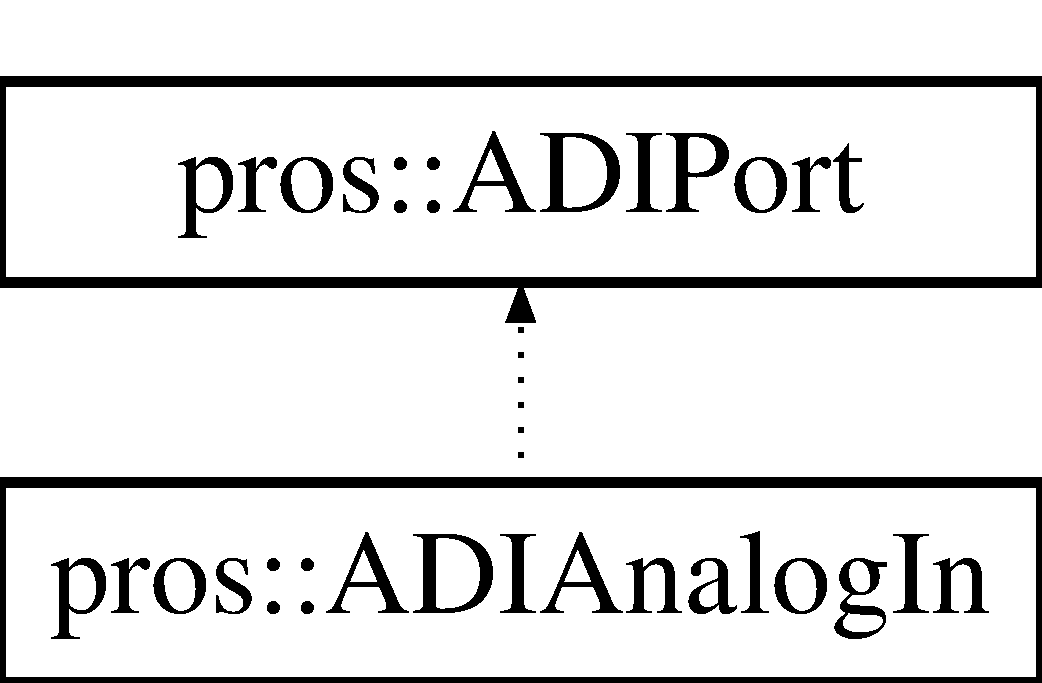
\includegraphics[height=2.000000cm]{classpros_1_1ADIAnalogIn}
\end{center}
\end{figure}
\subsection*{Public Member Functions}
\begin{DoxyCompactItemize}
\item 
\hyperlink{classpros_1_1ADIAnalogIn_aeac81958e7ba33ee9693ab843f5b55ed}{A\+D\+I\+Analog\+In} (std\+::uint8\+\_\+t port)
\item 
std\+::int32\+\_\+t \hyperlink{classpros_1_1ADIAnalogIn_ac8dd1e625cbcec4951d20be0c0fa2d3c}{calibrate} (void) const
\item 
std\+::int32\+\_\+t \hyperlink{classpros_1_1ADIAnalogIn_a5930ce87c880833bda8cd202613b8d80}{get\+\_\+value\+\_\+calibrated} (void) const
\item 
std\+::int32\+\_\+t \hyperlink{classpros_1_1ADIAnalogIn_a65bfed175ed1b0efce4566e78e7f9473}{get\+\_\+value\+\_\+calibrated\+\_\+\+HR} (void) const
\end{DoxyCompactItemize}


\subsection{Constructor \& Destructor Documentation}
\mbox{\Hypertarget{classpros_1_1ADIAnalogIn_aeac81958e7ba33ee9693ab843f5b55ed}\label{classpros_1_1ADIAnalogIn_aeac81958e7ba33ee9693ab843f5b55ed}} 
\index{pros\+::\+A\+D\+I\+Analog\+In@{pros\+::\+A\+D\+I\+Analog\+In}!A\+D\+I\+Analog\+In@{A\+D\+I\+Analog\+In}}
\index{A\+D\+I\+Analog\+In@{A\+D\+I\+Analog\+In}!pros\+::\+A\+D\+I\+Analog\+In@{pros\+::\+A\+D\+I\+Analog\+In}}
\subsubsection{\texorpdfstring{A\+D\+I\+Analog\+In()}{ADIAnalogIn()}}
{\footnotesize\ttfamily pros\+::\+A\+D\+I\+Analog\+In\+::\+A\+D\+I\+Analog\+In (\begin{DoxyParamCaption}\item[{std\+::uint8\+\_\+t}]{port }\end{DoxyParamCaption})}

Configures an A\+DI port to act as an Analog Input.

This function uses the following values of errno when an error state is reached\+: E\+N\+X\+IO -\/ The given value is not within the range of A\+DI Ports


\begin{DoxyParams}{Parameters}
{\em port} & The A\+DI port number (from 1-\/8, \textquotesingle{}a\textquotesingle{}-\/\textquotesingle{}h\textquotesingle{}, \textquotesingle{}A\textquotesingle{}-\/\textquotesingle{}H\textquotesingle{}) to configure \\
\hline
{\em type} & The configuration type for the port\\
\hline
\end{DoxyParams}
\begin{DoxyReturn}{Returns}
1 if the operation was successful or P\+R\+O\+S\+\_\+\+E\+RR if the operation failed, setting errno. 
\end{DoxyReturn}


\subsection{Member Function Documentation}
\mbox{\Hypertarget{classpros_1_1ADIAnalogIn_ac8dd1e625cbcec4951d20be0c0fa2d3c}\label{classpros_1_1ADIAnalogIn_ac8dd1e625cbcec4951d20be0c0fa2d3c}} 
\index{pros\+::\+A\+D\+I\+Analog\+In@{pros\+::\+A\+D\+I\+Analog\+In}!calibrate@{calibrate}}
\index{calibrate@{calibrate}!pros\+::\+A\+D\+I\+Analog\+In@{pros\+::\+A\+D\+I\+Analog\+In}}
\subsubsection{\texorpdfstring{calibrate()}{calibrate()}}
{\footnotesize\ttfamily std\+::int32\+\_\+t pros\+::\+A\+D\+I\+Analog\+In\+::calibrate (\begin{DoxyParamCaption}\item[{void}]{ }\end{DoxyParamCaption}) const}

Calibrates the analog sensor on the specified port and returns the new calibration value.

This method assumes that the true sensor value is not actively changing at this time and computes an average from approximately 500 samples, 1 ms apart, for a 0.\+5 s period of calibration. The average value thus calculated is returned and stored for later calls to the \hyperlink{classpros_1_1ADIAnalogIn_a5930ce87c880833bda8cd202613b8d80}{pros\+::\+A\+D\+I\+Analog\+In\+::get\+\_\+value\+\_\+calibrated()} and \hyperlink{classpros_1_1ADIAnalogIn_a65bfed175ed1b0efce4566e78e7f9473}{pros\+::\+A\+D\+I\+Analog\+In\+::get\+\_\+value\+\_\+calibrated\+\_\+\+H\+R()} functions. These functions will return the difference between this value and the current sensor value when called.

Do not use this function when the sensor value might be unstable (gyro rotation, accelerometer movement).

This function uses the following values of errno when an error state is reached\+: E\+N\+O\+D\+EV -\/ The port is not configured as an analog input

\begin{DoxyReturn}{Returns}
The average sensor value computed by this function 
\end{DoxyReturn}
\mbox{\Hypertarget{classpros_1_1ADIAnalogIn_a5930ce87c880833bda8cd202613b8d80}\label{classpros_1_1ADIAnalogIn_a5930ce87c880833bda8cd202613b8d80}} 
\index{pros\+::\+A\+D\+I\+Analog\+In@{pros\+::\+A\+D\+I\+Analog\+In}!get\+\_\+value\+\_\+calibrated@{get\+\_\+value\+\_\+calibrated}}
\index{get\+\_\+value\+\_\+calibrated@{get\+\_\+value\+\_\+calibrated}!pros\+::\+A\+D\+I\+Analog\+In@{pros\+::\+A\+D\+I\+Analog\+In}}
\subsubsection{\texorpdfstring{get\+\_\+value\+\_\+calibrated()}{get\_value\_calibrated()}}
{\footnotesize\ttfamily std\+::int32\+\_\+t pros\+::\+A\+D\+I\+Analog\+In\+::get\+\_\+value\+\_\+calibrated (\begin{DoxyParamCaption}\item[{void}]{ }\end{DoxyParamCaption}) const}

Gets the 12 bit calibrated value of an analog input port.

The \hyperlink{classpros_1_1ADIAnalogIn_ac8dd1e625cbcec4951d20be0c0fa2d3c}{pros\+::\+A\+D\+I\+Analog\+In\+::calibrate()} function must be run first. This function is inappropriate for sensor values intended for integration, as round-\/off error can accumulate causing drift over time. Use \hyperlink{classpros_1_1ADIAnalogIn_a65bfed175ed1b0efce4566e78e7f9473}{pros\+::\+A\+D\+I\+Analog\+In\+::get\+\_\+value\+\_\+calibrated\+\_\+\+H\+R()} instead.

This function uses the following values of errno when an error state is reached\+: E\+N\+O\+D\+EV -\/ The port is not configured as an analog input

\begin{DoxyReturn}{Returns}
The difference of the sensor value from its calibrated default from -\/4095 to 4095 
\end{DoxyReturn}
\mbox{\Hypertarget{classpros_1_1ADIAnalogIn_a65bfed175ed1b0efce4566e78e7f9473}\label{classpros_1_1ADIAnalogIn_a65bfed175ed1b0efce4566e78e7f9473}} 
\index{pros\+::\+A\+D\+I\+Analog\+In@{pros\+::\+A\+D\+I\+Analog\+In}!get\+\_\+value\+\_\+calibrated\+\_\+\+HR@{get\+\_\+value\+\_\+calibrated\+\_\+\+HR}}
\index{get\+\_\+value\+\_\+calibrated\+\_\+\+HR@{get\+\_\+value\+\_\+calibrated\+\_\+\+HR}!pros\+::\+A\+D\+I\+Analog\+In@{pros\+::\+A\+D\+I\+Analog\+In}}
\subsubsection{\texorpdfstring{get\+\_\+value\+\_\+calibrated\+\_\+\+H\+R()}{get\_value\_calibrated\_HR()}}
{\footnotesize\ttfamily std\+::int32\+\_\+t pros\+::\+A\+D\+I\+Analog\+In\+::get\+\_\+value\+\_\+calibrated\+\_\+\+HR (\begin{DoxyParamCaption}\item[{void}]{ }\end{DoxyParamCaption}) const}

Gets the 16 bit calibrated value of an analog input port.

The \hyperlink{classpros_1_1ADIAnalogIn_ac8dd1e625cbcec4951d20be0c0fa2d3c}{pros\+::\+A\+D\+I\+Analog\+In\+::calibrate()} function must be run first. This is intended for integrated sensor values such as gyros and accelerometers to reduce drift due to round-\/off, and should not be used on a sensor such as a line tracker or potentiometer.

The value returned actually has 16 bits of \char`\"{}precision\char`\"{}, even though the A\+DC only reads 12 bits, so that error induced by the average value being between two values when integrated over time is trivial. Think of the value as the true value times 16.

This function uses the following values of errno when an error state is reached\+: E\+N\+O\+D\+EV -\/ The port is not configured as an analog input

\begin{DoxyReturn}{Returns}
The difference of the sensor value from its calibrated default from -\/16384 to 16384 
\end{DoxyReturn}


The documentation for this class was generated from the following file\+:\begin{DoxyCompactItemize}
\item 
pros/include/pros/\hyperlink{adi_8hpp}{adi.\+hpp}\end{DoxyCompactItemize}

\hypertarget{classpros_1_1ADIAnalogOut}{}\section{pros\+:\+:A\+D\+I\+Analog\+Out Class Reference}
\label{classpros_1_1ADIAnalogOut}\index{pros\+::\+A\+D\+I\+Analog\+Out@{pros\+::\+A\+D\+I\+Analog\+Out}}


{\ttfamily \#include $<$adi.\+hpp$>$}

Inheritance diagram for pros\+:\+:A\+D\+I\+Analog\+Out\+:\begin{figure}[H]
\begin{center}
\leavevmode
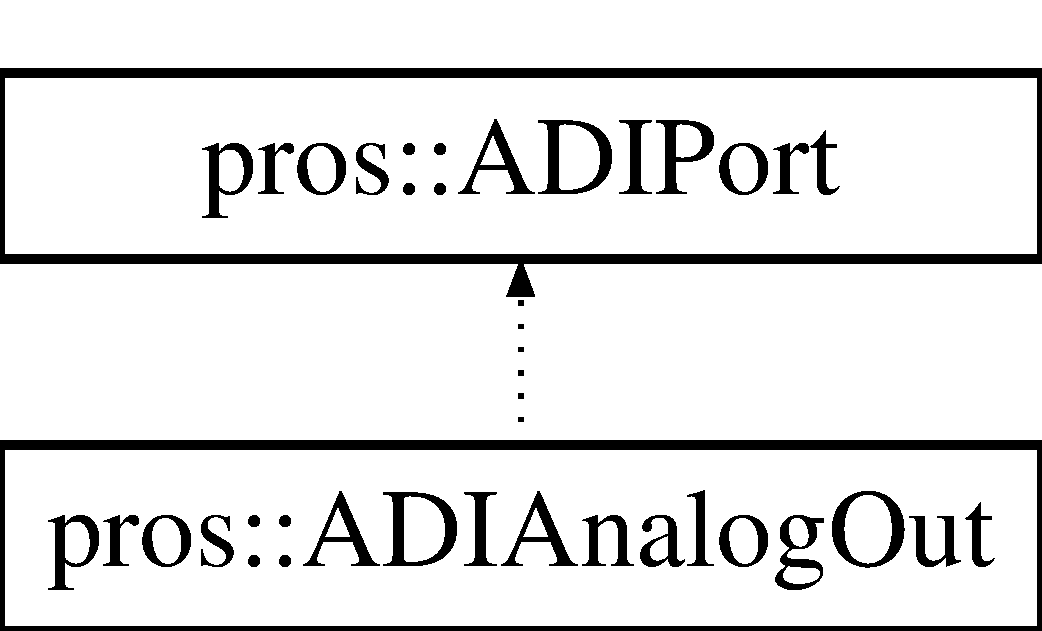
\includegraphics[height=2.000000cm]{classpros_1_1ADIAnalogOut}
\end{center}
\end{figure}
\subsection*{Public Member Functions}
\begin{DoxyCompactItemize}
\item 
\hyperlink{classpros_1_1ADIAnalogOut_a1758096961a060dea379bd696c293d26}{A\+D\+I\+Analog\+Out} (std\+::uint8\+\_\+t port)
\end{DoxyCompactItemize}


\subsection{Constructor \& Destructor Documentation}
\mbox{\Hypertarget{classpros_1_1ADIAnalogOut_a1758096961a060dea379bd696c293d26}\label{classpros_1_1ADIAnalogOut_a1758096961a060dea379bd696c293d26}} 
\index{pros\+::\+A\+D\+I\+Analog\+Out@{pros\+::\+A\+D\+I\+Analog\+Out}!A\+D\+I\+Analog\+Out@{A\+D\+I\+Analog\+Out}}
\index{A\+D\+I\+Analog\+Out@{A\+D\+I\+Analog\+Out}!pros\+::\+A\+D\+I\+Analog\+Out@{pros\+::\+A\+D\+I\+Analog\+Out}}
\subsubsection{\texorpdfstring{A\+D\+I\+Analog\+Out()}{ADIAnalogOut()}}
{\footnotesize\ttfamily pros\+::\+A\+D\+I\+Analog\+Out\+::\+A\+D\+I\+Analog\+Out (\begin{DoxyParamCaption}\item[{std\+::uint8\+\_\+t}]{port }\end{DoxyParamCaption})}

Configures an A\+DI port to act as an Analog Output.

This function uses the following values of errno when an error state is reached\+: E\+N\+X\+IO -\/ The given value is not within the range of A\+DI Ports.


\begin{DoxyParams}{Parameters}
{\em port} & The A\+DI port number (from 1-\/8, \textquotesingle{}a\textquotesingle{}-\/\textquotesingle{}h\textquotesingle{}, \textquotesingle{}A\textquotesingle{}-\/\textquotesingle{}H\textquotesingle{}) to configure \\
\hline
{\em type} & The configuration type for the port \\
\hline
\end{DoxyParams}


The documentation for this class was generated from the following file\+:\begin{DoxyCompactItemize}
\item 
pros/include/pros/\hyperlink{adi_8hpp}{adi.\+hpp}\end{DoxyCompactItemize}

\hypertarget{classpros_1_1ADIDigitalIn}{}\doxysection{A\+D\+I\+Digital\+In Class Reference}
\label{classpros_1_1ADIDigitalIn}\index{ADIDigitalIn@{ADIDigitalIn}}


{\ttfamily \#include \char`\"{}adi.\+hpp\char`\"{}}

Inheritance diagram for A\+D\+I\+Digital\+In\+:\begin{figure}[H]
\begin{center}
\leavevmode
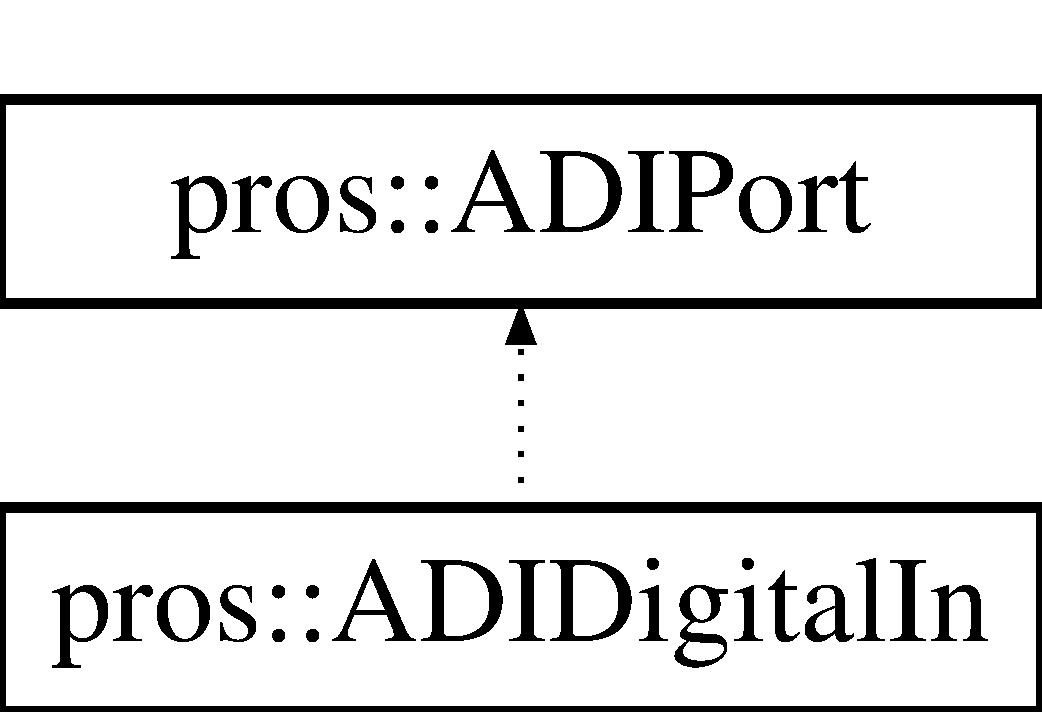
\includegraphics[height=2.000000cm]{classpros_1_1ADIDigitalIn}
\end{center}
\end{figure}
\doxysubsection*{Public Member Functions}
\begin{DoxyCompactItemize}
\item 
\mbox{\hyperlink{classpros_1_1ADIDigitalIn_a55442b68e310a25fcc6d34ae5c9fc1a0}{A\+D\+I\+Digital\+In}} (std\+::uint8\+\_\+t adi\+\_\+port)
\begin{DoxyCompactList}\small\item\em Configures an A\+DI port to act as a Digital Input. \end{DoxyCompactList}\item 
\mbox{\hyperlink{classpros_1_1ADIDigitalIn_af84801ff6a9b610a23f47bc54846cad4}{A\+D\+I\+Digital\+In}} (\mbox{\hyperlink{namespacepros_aa8b90563c470741ebd760aeacfd90599}{ext\+\_\+adi\+\_\+port\+\_\+pair\+\_\+t}} port\+\_\+pair)
\begin{DoxyCompactList}\small\item\em Configures an A\+DI port on an adi\+\_\+expander to act as a Digital Input. \end{DoxyCompactList}\item 
std\+::int32\+\_\+t \mbox{\hyperlink{classpros_1_1ADIDigitalIn_aecb46342cef79b5e76b1725996088abe}{get\+\_\+new\+\_\+press}} () const
\begin{DoxyCompactList}\small\item\em Gets a rising-\/edge case for a digital button press. \end{DoxyCompactList}\item 
std\+::int32\+\_\+t \mbox{\hyperlink{classpros_1_1ADIDigitalIn_a60987c8e4946650cf9aa40f8e8345f01}{get\+\_\+value}} () const
\begin{DoxyCompactList}\small\item\em Gets the value for the given A\+DI port. \end{DoxyCompactList}\end{DoxyCompactItemize}


\doxysubsection{Constructor \& Destructor Documentation}
\mbox{\Hypertarget{classpros_1_1ADIDigitalIn_a55442b68e310a25fcc6d34ae5c9fc1a0}\label{classpros_1_1ADIDigitalIn_a55442b68e310a25fcc6d34ae5c9fc1a0}} 
\index{ADIDigitalIn@{ADIDigitalIn}!ADIDigitalIn@{ADIDigitalIn}}
\index{ADIDigitalIn@{ADIDigitalIn}!ADIDigitalIn@{ADIDigitalIn}}
\doxysubsubsection{\texorpdfstring{ADIDigitalIn()}{ADIDigitalIn()}\hspace{0.1cm}{\footnotesize\ttfamily [1/2]}}
{\footnotesize\ttfamily \mbox{\hyperlink{classpros_1_1ADIDigitalIn}{A\+D\+I\+Digital\+In}} (\begin{DoxyParamCaption}\item[{std\+::uint8\+\_\+t}]{adi\+\_\+port }\end{DoxyParamCaption})\hspace{0.3cm}{\ttfamily [explicit]}}



Configures an A\+DI port to act as a Digital Input. 

This function uses the following values of errno when an error state is reached\+: E\+N\+X\+IO -\/ Either the A\+DI port value or the smart port value is not within its valid range (A\+DI port\+: 1-\/8, \textquotesingle{}a\textquotesingle{}-\/\textquotesingle{}h\textquotesingle{}, or \textquotesingle{}A\textquotesingle{}-\/\textquotesingle{}H\textquotesingle{}; smart port\+: 1-\/21).


\begin{DoxyParams}{Parameters}
{\em adi\+\_\+port} & The A\+DI port number (from 1-\/8, \textquotesingle{}a\textquotesingle{}-\/\textquotesingle{}h\textquotesingle{}, \textquotesingle{}A\textquotesingle{}-\/\textquotesingle{}H\textquotesingle{}) to configure \\
\hline
\end{DoxyParams}
\mbox{\Hypertarget{classpros_1_1ADIDigitalIn_af84801ff6a9b610a23f47bc54846cad4}\label{classpros_1_1ADIDigitalIn_af84801ff6a9b610a23f47bc54846cad4}} 
\index{ADIDigitalIn@{ADIDigitalIn}!ADIDigitalIn@{ADIDigitalIn}}
\index{ADIDigitalIn@{ADIDigitalIn}!ADIDigitalIn@{ADIDigitalIn}}
\doxysubsubsection{\texorpdfstring{ADIDigitalIn()}{ADIDigitalIn()}\hspace{0.1cm}{\footnotesize\ttfamily [2/2]}}
{\footnotesize\ttfamily \mbox{\hyperlink{classpros_1_1ADIDigitalIn}{A\+D\+I\+Digital\+In}} (\begin{DoxyParamCaption}\item[{\mbox{\hyperlink{namespacepros_aa8b90563c470741ebd760aeacfd90599}{ext\+\_\+adi\+\_\+port\+\_\+pair\+\_\+t}}}]{port\+\_\+pair }\end{DoxyParamCaption})}



Configures an A\+DI port on an adi\+\_\+expander to act as a Digital Input. 

This function uses the following values of errno when an error state is reached\+: E\+N\+X\+IO -\/ Either the A\+DI port value or the smart port value is not within its valid range (A\+DI port\+: 1-\/8, \textquotesingle{}a\textquotesingle{}-\/\textquotesingle{}h\textquotesingle{}, or \textquotesingle{}A\textquotesingle{}-\/\textquotesingle{}H\textquotesingle{}; smart port\+: 1-\/21).


\begin{DoxyParams}{Parameters}
{\em port\+\_\+pair} & The pair of the smart port number (from 1-\/22) and the A\+DI port number (from 1-\/8, \textquotesingle{}a\textquotesingle{}-\/\textquotesingle{}h\textquotesingle{}, \textquotesingle{}A\textquotesingle{}-\/\textquotesingle{}H\textquotesingle{}) to configure \\
\hline
\end{DoxyParams}


\doxysubsection{Member Function Documentation}
\mbox{\Hypertarget{classpros_1_1ADIDigitalIn_aecb46342cef79b5e76b1725996088abe}\label{classpros_1_1ADIDigitalIn_aecb46342cef79b5e76b1725996088abe}} 
\index{ADIDigitalIn@{ADIDigitalIn}!get\_new\_press@{get\_new\_press}}
\index{get\_new\_press@{get\_new\_press}!ADIDigitalIn@{ADIDigitalIn}}
\doxysubsubsection{\texorpdfstring{get\_new\_press()}{get\_new\_press()}}
{\footnotesize\ttfamily std\+::int32\+\_\+t get\+\_\+new\+\_\+press (\begin{DoxyParamCaption}{ }\end{DoxyParamCaption}) const}



Gets a rising-\/edge case for a digital button press. 

This function is not thread-\/safe. Multiple tasks polling a single button may return different results under the same circumstances, so only one task should call this function for any given button. E.\+g., \mbox{\hyperlink{classpros_1_1Task}{Task}} A calls this function for buttons 1 and 2. \mbox{\hyperlink{classpros_1_1Task}{Task}} B may call this function for button 3, but should not for buttons 1 or 2. A typical use-\/case for this function is to call inside opcontrol to detect new button presses, and not in any other tasks.

This function uses the following values of errno when an error state is reached\+: E\+N\+O\+D\+EV -\/ The port is not configured as a digital input

\begin{DoxyReturn}{Returns}
1 if the button is pressed and had not been pressed the last time this function was called, 0 otherwise. 
\end{DoxyReturn}
\mbox{\Hypertarget{classpros_1_1ADIDigitalIn_a60987c8e4946650cf9aa40f8e8345f01}\label{classpros_1_1ADIDigitalIn_a60987c8e4946650cf9aa40f8e8345f01}} 
\index{ADIDigitalIn@{ADIDigitalIn}!get\_value@{get\_value}}
\index{get\_value@{get\_value}!ADIDigitalIn@{ADIDigitalIn}}
\doxysubsubsection{\texorpdfstring{get\_value()}{get\_value()}}
{\footnotesize\ttfamily std\+::int32\+\_\+t get\+\_\+value}



Gets the value for the given A\+DI port. 

This function uses the following values of errno when an error state is reached\+: E\+N\+O\+D\+EV -\/ The port is not configured as a digital input

\begin{DoxyReturn}{Returns}
The value stored for the given port 
\end{DoxyReturn}


The documentation for this class was generated from the following file\+:\begin{DoxyCompactItemize}
\item 
pros/\mbox{\hyperlink{adi_8hpp}{adi.\+hpp}}\end{DoxyCompactItemize}

\hypertarget{classpros_1_1ADIDigitalOut}{}\doxysection{A\+D\+I\+Digital\+Out Class Reference}
\label{classpros_1_1ADIDigitalOut}\index{ADIDigitalOut@{ADIDigitalOut}}


{\ttfamily \#include \char`\"{}adi.\+hpp\char`\"{}}

Inheritance diagram for A\+D\+I\+Digital\+Out\+:\begin{figure}[H]
\begin{center}
\leavevmode
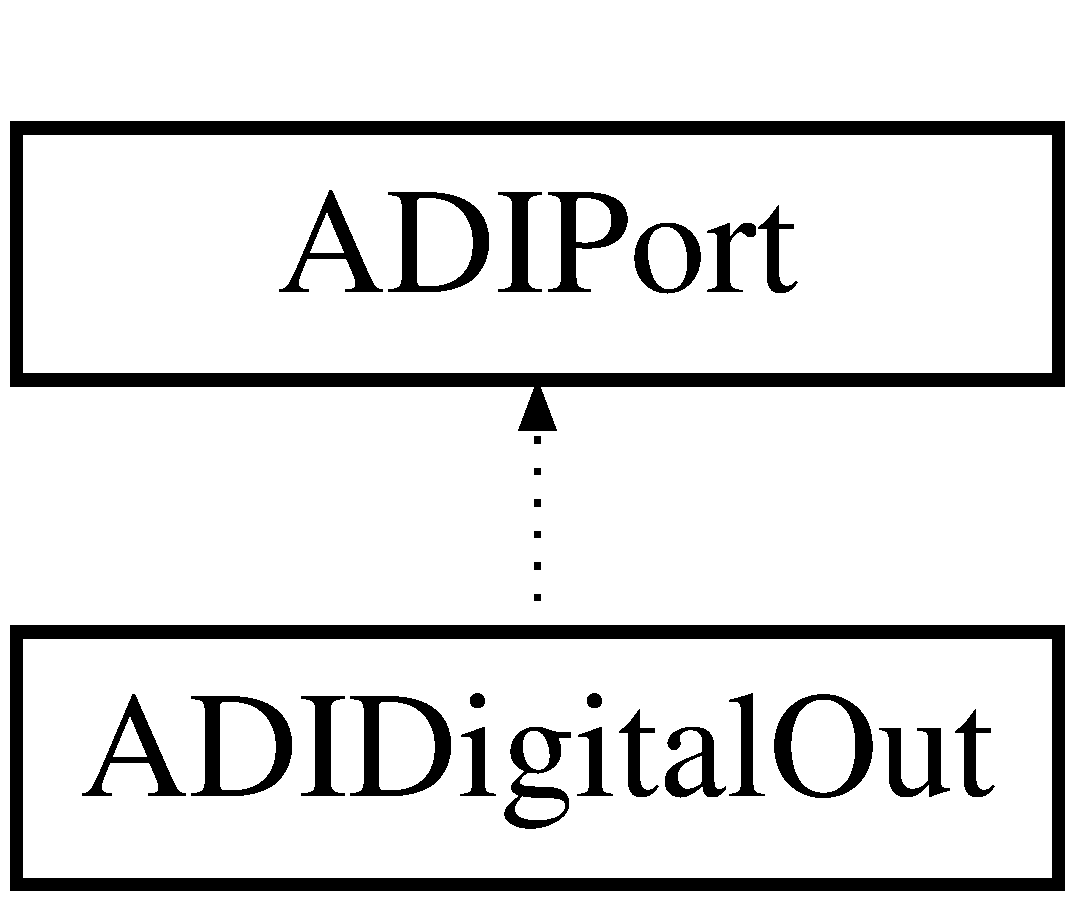
\includegraphics[height=2.000000cm]{classpros_1_1ADIDigitalOut}
\end{center}
\end{figure}
\doxysubsection*{Public Member Functions}
\begin{DoxyCompactItemize}
\item 
\mbox{\hyperlink{group__cpp-adi_gaace6711643eedf7f140d3af34da7bfa6}{A\+D\+I\+Digital\+Out}} (std\+::uint8\+\_\+t adi\+\_\+port, bool init\+\_\+state=\mbox{\hyperlink{group__c-adi_gab811d8c6ff3a505312d3276590444289}{L\+OW}})
\begin{DoxyCompactList}\small\item\em Configures an A\+DI port to act as a Digital Output. \end{DoxyCompactList}\item 
\mbox{\hyperlink{group__cpp-adi_gab2912f0fe6ad3c664391d90febe4fc98}{A\+D\+I\+Digital\+Out}} (\mbox{\hyperlink{namespacepros_aa8b90563c470741ebd760aeacfd90599}{ext\+\_\+adi\+\_\+port\+\_\+pair\+\_\+t}} port\+\_\+pair, bool init\+\_\+state=\mbox{\hyperlink{group__c-adi_gab811d8c6ff3a505312d3276590444289}{L\+OW}})
\begin{DoxyCompactList}\small\item\em Configures an A\+DI port on an adi\+\_\+expander to act as a Digital Output. \end{DoxyCompactList}\item 
std\+::int32\+\_\+t \mbox{\hyperlink{classpros_1_1ADIDigitalOut_a833ed782b711495035dae08cfce3e62e}{set\+\_\+value}} (std\+::int32\+\_\+t value) const
\begin{DoxyCompactList}\small\item\em Sets the digital value (1 or 0) of a pin. \end{DoxyCompactList}\end{DoxyCompactItemize}


\doxysubsection{Member Function Documentation}
\mbox{\Hypertarget{classpros_1_1ADIDigitalOut_a833ed782b711495035dae08cfce3e62e}\label{classpros_1_1ADIDigitalOut_a833ed782b711495035dae08cfce3e62e}} 
\index{ADIDigitalOut@{ADIDigitalOut}!set\_value@{set\_value}}
\index{set\_value@{set\_value}!ADIDigitalOut@{ADIDigitalOut}}
\doxysubsubsection{\texorpdfstring{set\_value()}{set\_value()}}
{\footnotesize\ttfamily std\+::int32\+\_\+t set\+\_\+value}



Sets the digital value (1 or 0) of a pin. 

Inherited from \mbox{\hyperlink{group__cpp-adi_ga833ed782b711495035dae08cfce3e62e}{A\+D\+I\+Port\+::set\+\_\+value}}.

This function uses the following values of errno when an error state is reached\+: E\+A\+D\+D\+R\+I\+N\+U\+SE -\/ The port is not configured as a digital output (e.\+g. the port has been reconfigured)


\begin{DoxyParams}{Parameters}
{\em value} & The value to set the A\+DI port to\\
\hline
\end{DoxyParams}
\begin{DoxyReturn}{Returns}
if the operation was successful or P\+R\+O\+S\+\_\+\+E\+RR if the operation failed, setting errno.
\end{DoxyReturn}
{\bfseries{Example}} 
\begin{DoxyCode}{0}
\DoxyCodeLine{\textcolor{preprocessor}{\#define DIGITAL\_SENSOR\_PORT 1}}
\DoxyCodeLine{}
\DoxyCodeLine{\textcolor{keywordtype}{void} \mbox{\hyperlink{main_8h_a1903abdb5ef0f301d660754c8315fc17}{opcontrol}}() \{}
\DoxyCodeLine{  \textcolor{keywordtype}{bool} state = \mbox{\hyperlink{group__c-adi_gab811d8c6ff3a505312d3276590444289}{LOW}};}
\DoxyCodeLine{  \mbox{\hyperlink{classpros_1_1ADIDigitalOut}{pros::ADIDigitalOut}} sensor (DIGITAL\_SENSOR\_PORT);}
\DoxyCodeLine{  \textcolor{keywordflow}{while} (\textcolor{keyword}{true}) \{}
\DoxyCodeLine{    state != state;}
\DoxyCodeLine{    sensor.set\_value(state);}
\DoxyCodeLine{    \mbox{\hyperlink{group__c-llemu_ga6a62f5325d65f95436762552df547d73}{pros::delay}}(10); \textcolor{comment}{// toggle the sensor value every 50ms}}
\DoxyCodeLine{  \}}
\DoxyCodeLine{\}}
\end{DoxyCode}
 

The documentation for this class was generated from the following file\+:\begin{DoxyCompactItemize}
\item 
pros/\mbox{\hyperlink{adi_8hpp}{adi.\+hpp}}\end{DoxyCompactItemize}

\hypertarget{classpros_1_1ADIEncoder}{}\doxysection{ADIEncoder Class Reference}
\label{classpros_1_1ADIEncoder}\index{ADIEncoder@{ADIEncoder}}


{\ttfamily \#include \char`\"{}adi.\+hpp\char`\"{}}

Inheritance diagram for ADIEncoder\+:\begin{figure}[H]
\begin{center}
\leavevmode
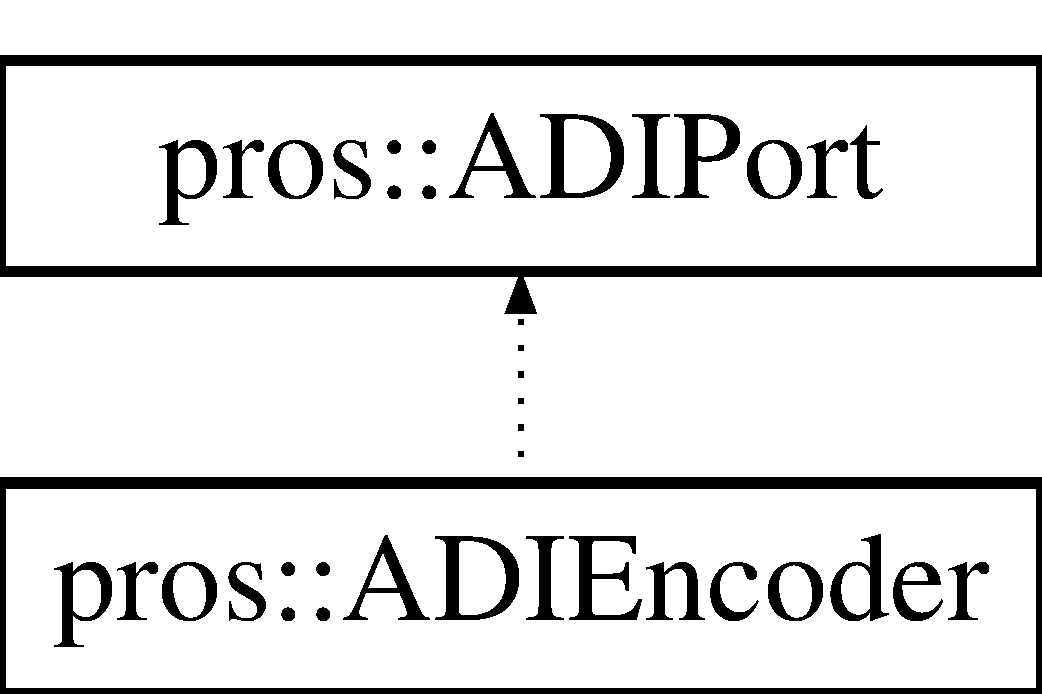
\includegraphics[height=2.000000cm]{classpros_1_1ADIEncoder}
\end{center}
\end{figure}
\doxysubsection*{Public Member Functions}
\begin{DoxyCompactItemize}
\item 
\mbox{\hyperlink{classpros_1_1ADIEncoder_a8e4997e865213b80c2b807f94d4f2d5c}{ADIEncoder}} (std\+::uint8\+\_\+t adi\+\_\+port\+\_\+top, std\+::uint8\+\_\+t adi\+\_\+port\+\_\+bottom, bool reversed=false)
\begin{DoxyCompactList}\small\item\em Configures a set of ADI ports to act as an Encoder. \end{DoxyCompactList}\item 
\mbox{\hyperlink{classpros_1_1ADIEncoder_a1866c137d27015ab24a4ba7554118353}{ADIEncoder}} (\mbox{\hyperlink{namespacepros_ab96eeca6120dfe95a7a63bbe88723f3e}{ext\+\_\+adi\+\_\+port\+\_\+tuple\+\_\+t}} port\+\_\+tuple, bool reversed=false)
\begin{DoxyCompactList}\small\item\em Configures a set of ADI ports on an adi\+\_\+expander to act as an Encoder. \end{DoxyCompactList}\item 
std\+::int32\+\_\+t \mbox{\hyperlink{classpros_1_1ADIEncoder_ac92589176d26914068b37bb9d6afba7b}{reset}} () const
\begin{DoxyCompactList}\small\item\em Sets the encoder value to zero. \end{DoxyCompactList}\item 
std\+::int32\+\_\+t \mbox{\hyperlink{classpros_1_1ADIEncoder_a60987c8e4946650cf9aa40f8e8345f01}{get\+\_\+value}} () const
\begin{DoxyCompactList}\small\item\em Gets the number of ticks recorded by the encoder. \end{DoxyCompactList}\end{DoxyCompactItemize}


\doxysubsection{Constructor \& Destructor Documentation}
\mbox{\Hypertarget{classpros_1_1ADIEncoder_a8e4997e865213b80c2b807f94d4f2d5c}\label{classpros_1_1ADIEncoder_a8e4997e865213b80c2b807f94d4f2d5c}} 
\index{ADIEncoder@{ADIEncoder}!ADIEncoder@{ADIEncoder}}
\index{ADIEncoder@{ADIEncoder}!ADIEncoder@{ADIEncoder}}
\doxysubsubsection{\texorpdfstring{ADIEncoder()}{ADIEncoder()}\hspace{0.1cm}{\footnotesize\ttfamily [1/2]}}
{\footnotesize\ttfamily \mbox{\hyperlink{classpros_1_1ADIEncoder}{ADIEncoder}} (\begin{DoxyParamCaption}\item[{std\+::uint8\+\_\+t}]{adi\+\_\+port\+\_\+top,  }\item[{std\+::uint8\+\_\+t}]{adi\+\_\+port\+\_\+bottom,  }\item[{bool}]{reversed = {\ttfamily false} }\end{DoxyParamCaption})}



Configures a set of ADI ports to act as an Encoder. 

This function uses the following values of errno when an error state is reached\+: ENXIO -\/ Either the ADI port value or the smart port value is not within its valid range (ADI port\+: 1-\/8, \textquotesingle{}a\textquotesingle{}-\/\textquotesingle{}h\textquotesingle{}, or \textquotesingle{}A\textquotesingle{}-\/\textquotesingle{}H\textquotesingle{}; smart port\+: 1-\/21).


\begin{DoxyParams}{Parameters}
{\em adi\+\_\+port\+\_\+top} & The \char`\"{}top\char`\"{} wire from the encoder sensor with the removable cover side up \\
\hline
{\em adi\+\_\+port\+\_\+bottom} & The \char`\"{}bottom\char`\"{} wire from the encoder sensor \\
\hline
{\em reverse} & If \char`\"{}true\char`\"{}, the sensor will count in the opposite direction \\
\hline
\end{DoxyParams}
\mbox{\Hypertarget{classpros_1_1ADIEncoder_a1866c137d27015ab24a4ba7554118353}\label{classpros_1_1ADIEncoder_a1866c137d27015ab24a4ba7554118353}} 
\index{ADIEncoder@{ADIEncoder}!ADIEncoder@{ADIEncoder}}
\index{ADIEncoder@{ADIEncoder}!ADIEncoder@{ADIEncoder}}
\doxysubsubsection{\texorpdfstring{ADIEncoder()}{ADIEncoder()}\hspace{0.1cm}{\footnotesize\ttfamily [2/2]}}
{\footnotesize\ttfamily \mbox{\hyperlink{classpros_1_1ADIEncoder}{ADIEncoder}} (\begin{DoxyParamCaption}\item[{\mbox{\hyperlink{namespacepros_ab96eeca6120dfe95a7a63bbe88723f3e}{ext\+\_\+adi\+\_\+port\+\_\+tuple\+\_\+t}}}]{port\+\_\+tuple,  }\item[{bool}]{reversed = {\ttfamily false} }\end{DoxyParamCaption})}



Configures a set of ADI ports on an adi\+\_\+expander to act as an Encoder. 

This function uses the following values of errno when an error state is reached\+: ENXIO -\/ Either the ADI port value or the smart port value is not within its valid range (ADI port\+: 1-\/8, \textquotesingle{}a\textquotesingle{}-\/\textquotesingle{}h\textquotesingle{}, or \textquotesingle{}A\textquotesingle{}-\/\textquotesingle{}H\textquotesingle{}; smart port\+: 1-\/21).


\begin{DoxyParams}{Parameters}
{\em port\+\_\+tuple} & The tuple of the smart port number, the \char`\"{}top\char`\"{} wire from the encoder sensor with the removable cover side up, and the \char`\"{}bottom\char`\"{} wire from the encoder sensor \\
\hline
{\em reverse} & If \char`\"{}true\char`\"{}, the sensor will count in theopposite direction \\
\hline
\end{DoxyParams}


\doxysubsection{Member Function Documentation}
\mbox{\Hypertarget{classpros_1_1ADIEncoder_ac92589176d26914068b37bb9d6afba7b}\label{classpros_1_1ADIEncoder_ac92589176d26914068b37bb9d6afba7b}} 
\index{ADIEncoder@{ADIEncoder}!reset@{reset}}
\index{reset@{reset}!ADIEncoder@{ADIEncoder}}
\doxysubsubsection{\texorpdfstring{reset()}{reset()}}
{\footnotesize\ttfamily std\+::int32\+\_\+t reset (\begin{DoxyParamCaption}{ }\end{DoxyParamCaption}) const}



Sets the encoder value to zero. 

It is safe to use this method while an encoder is enabled. It is not necessary to call this method before stopping or starting an encoder.

This function uses the following values of errno when an error state is reached\+: ENODEV -\/ The port is not configured as a motor

\begin{DoxyReturn}{Returns}
1 if the operation was successful or PROS\+\_\+\+ERR if the operation failed, setting errno. 
\end{DoxyReturn}
\mbox{\Hypertarget{classpros_1_1ADIEncoder_a60987c8e4946650cf9aa40f8e8345f01}\label{classpros_1_1ADIEncoder_a60987c8e4946650cf9aa40f8e8345f01}} 
\index{ADIEncoder@{ADIEncoder}!get\_value@{get\_value}}
\index{get\_value@{get\_value}!ADIEncoder@{ADIEncoder}}
\doxysubsubsection{\texorpdfstring{get\_value()}{get\_value()}}
{\footnotesize\ttfamily std\+::int32\+\_\+t get\+\_\+value (\begin{DoxyParamCaption}{ }\end{DoxyParamCaption}) const}



Gets the number of ticks recorded by the encoder. 

There are 360 ticks in one revolution.

This function uses the following values of errno when an error state is reached\+: ENODEV -\/ The port is not configured as a motor

\begin{DoxyReturn}{Returns}
The signed and cumulative number of counts since the last start or reset 
\end{DoxyReturn}


The documentation for this class was generated from the following file\+:\begin{DoxyCompactItemize}
\item 
pros/\mbox{\hyperlink{adi_8hpp}{adi.\+hpp}}\end{DoxyCompactItemize}

\hypertarget{classpros_1_1ADIGyro}{}\section{pros\+:\+:A\+D\+I\+Gyro Class Reference}
\label{classpros_1_1ADIGyro}\index{pros\+::\+A\+D\+I\+Gyro@{pros\+::\+A\+D\+I\+Gyro}}


{\ttfamily \#include $<$adi.\+hpp$>$}

Inheritance diagram for pros\+:\+:A\+D\+I\+Gyro\+:\begin{figure}[H]
\begin{center}
\leavevmode
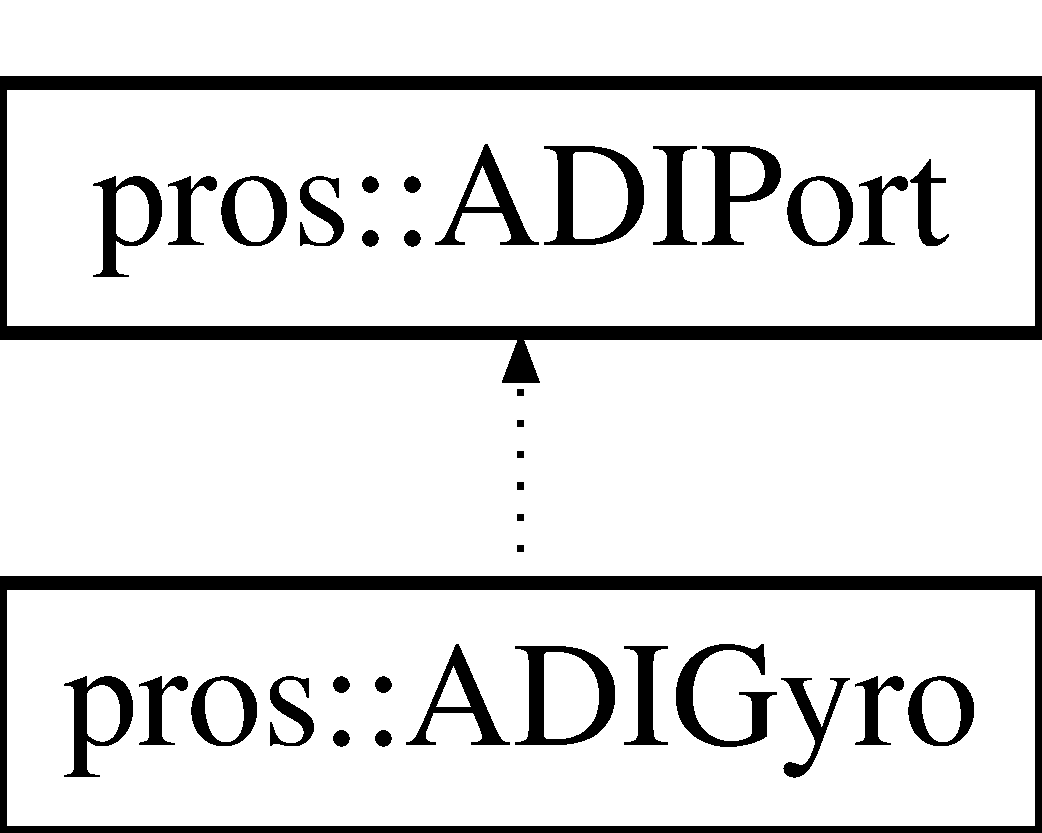
\includegraphics[height=2.000000cm]{classpros_1_1ADIGyro}
\end{center}
\end{figure}
\subsection*{Public Member Functions}
\begin{DoxyCompactItemize}
\item 
\hyperlink{classpros_1_1ADIGyro_adc826b3bcb88213a0df283178279662a}{A\+D\+I\+Gyro} (std\+::uint8\+\_\+t port, double multiplier=1)
\item 
double \hyperlink{classpros_1_1ADIGyro_a829f933aaaa370483c36aba9f4a4f09c}{get\+\_\+value} (void) const
\item 
std\+::int32\+\_\+t \hyperlink{classpros_1_1ADIGyro_a3e2df8c21f4eb0bfa3559834221195fe}{reset} (void) const
\end{DoxyCompactItemize}


\subsection{Constructor \& Destructor Documentation}
\mbox{\Hypertarget{classpros_1_1ADIGyro_adc826b3bcb88213a0df283178279662a}\label{classpros_1_1ADIGyro_adc826b3bcb88213a0df283178279662a}} 
\index{pros\+::\+A\+D\+I\+Gyro@{pros\+::\+A\+D\+I\+Gyro}!A\+D\+I\+Gyro@{A\+D\+I\+Gyro}}
\index{A\+D\+I\+Gyro@{A\+D\+I\+Gyro}!pros\+::\+A\+D\+I\+Gyro@{pros\+::\+A\+D\+I\+Gyro}}
\subsubsection{\texorpdfstring{A\+D\+I\+Gyro()}{ADIGyro()}}
{\footnotesize\ttfamily pros\+::\+A\+D\+I\+Gyro\+::\+A\+D\+I\+Gyro (\begin{DoxyParamCaption}\item[{std\+::uint8\+\_\+t}]{port,  }\item[{double}]{multiplier = {\ttfamily 1} }\end{DoxyParamCaption})}

Initializes a gyroscope on the given port. If the given port has not previously been configured as a gyro, then this function starts a 1300ms calibration period.

It is highly recommended that an \hyperlink{classpros_1_1ADIGyro}{A\+D\+I\+Gyro} object be created in \hyperlink{main_8h_a9efe22aaead3a5e936b5df459de02eba}{initialize()} when the robot is stationary to ensure proper calibration. If an \hyperlink{classpros_1_1ADIGyro}{A\+D\+I\+Gyro} object is declared at the global scope, a hardcoded 1300ms delay at the beginning of initialize will be necessary to ensure that the gyro\textquotesingle{}s returned values are correct at the beginning of autonomous/opcontrol.

This function uses the following values of errno when an error state is reached\+: E\+N\+X\+IO -\/ The given value is not within the range of A\+DI Ports


\begin{DoxyParams}{Parameters}
{\em port} & The A\+DI port to initialize as a gyro (from 1-\/8, \textquotesingle{}a\textquotesingle{}-\/\textquotesingle{}h\textquotesingle{}, \textquotesingle{}A\textquotesingle{}-\/\textquotesingle{}H\textquotesingle{}) \\
\hline
{\em multiplier} & A scalar value that will be multiplied by the gyro heading value supplied by the A\+DI \\
\hline
\end{DoxyParams}


\subsection{Member Function Documentation}
\mbox{\Hypertarget{classpros_1_1ADIGyro_a829f933aaaa370483c36aba9f4a4f09c}\label{classpros_1_1ADIGyro_a829f933aaaa370483c36aba9f4a4f09c}} 
\index{pros\+::\+A\+D\+I\+Gyro@{pros\+::\+A\+D\+I\+Gyro}!get\+\_\+value@{get\+\_\+value}}
\index{get\+\_\+value@{get\+\_\+value}!pros\+::\+A\+D\+I\+Gyro@{pros\+::\+A\+D\+I\+Gyro}}
\subsubsection{\texorpdfstring{get\+\_\+value()}{get\_value()}}
{\footnotesize\ttfamily double pros\+::\+A\+D\+I\+Gyro\+::get\+\_\+value (\begin{DoxyParamCaption}\item[{void}]{ }\end{DoxyParamCaption}) const}

Gets the current gyro angle in tenths of a degree. Unless a multiplier is applied to the gyro, the return value will be a whole number representing the number of degrees of rotation times 10.

There are 360 degrees in a circle, thus the gyro will return 3600 for one whole rotation.

This function uses the following values of errno when an error state is reached\+: E\+N\+O\+D\+EV -\/ The port is not configured as a gyro

\begin{DoxyReturn}{Returns}
The gyro angle in degrees. 
\end{DoxyReturn}
\mbox{\Hypertarget{classpros_1_1ADIGyro_a3e2df8c21f4eb0bfa3559834221195fe}\label{classpros_1_1ADIGyro_a3e2df8c21f4eb0bfa3559834221195fe}} 
\index{pros\+::\+A\+D\+I\+Gyro@{pros\+::\+A\+D\+I\+Gyro}!reset@{reset}}
\index{reset@{reset}!pros\+::\+A\+D\+I\+Gyro@{pros\+::\+A\+D\+I\+Gyro}}
\subsubsection{\texorpdfstring{reset()}{reset()}}
{\footnotesize\ttfamily std\+::int32\+\_\+t pros\+::\+A\+D\+I\+Gyro\+::reset (\begin{DoxyParamCaption}\item[{void}]{ }\end{DoxyParamCaption}) const}

Resets the gyroscope value to zero.

This function uses the following values of errno when an error state is reached\+: E\+N\+O\+D\+EV -\/ The port is not configured as a gyro

\begin{DoxyReturn}{Returns}
1 if the operation was successful or P\+R\+O\+S\+\_\+\+E\+RR if the operation failed, setting errno. 
\end{DoxyReturn}


The documentation for this class was generated from the following file\+:\begin{DoxyCompactItemize}
\item 
pros/include/pros/\hyperlink{adi_8hpp}{adi.\+hpp}\end{DoxyCompactItemize}

\hypertarget{classpros_1_1ADIMotor}{}\section{pros\+:\+:A\+D\+I\+Motor Class Reference}
\label{classpros_1_1ADIMotor}\index{pros\+::\+A\+D\+I\+Motor@{pros\+::\+A\+D\+I\+Motor}}


{\ttfamily \#include $<$adi.\+hpp$>$}

Inheritance diagram for pros\+:\+:A\+D\+I\+Motor\+:\begin{figure}[H]
\begin{center}
\leavevmode
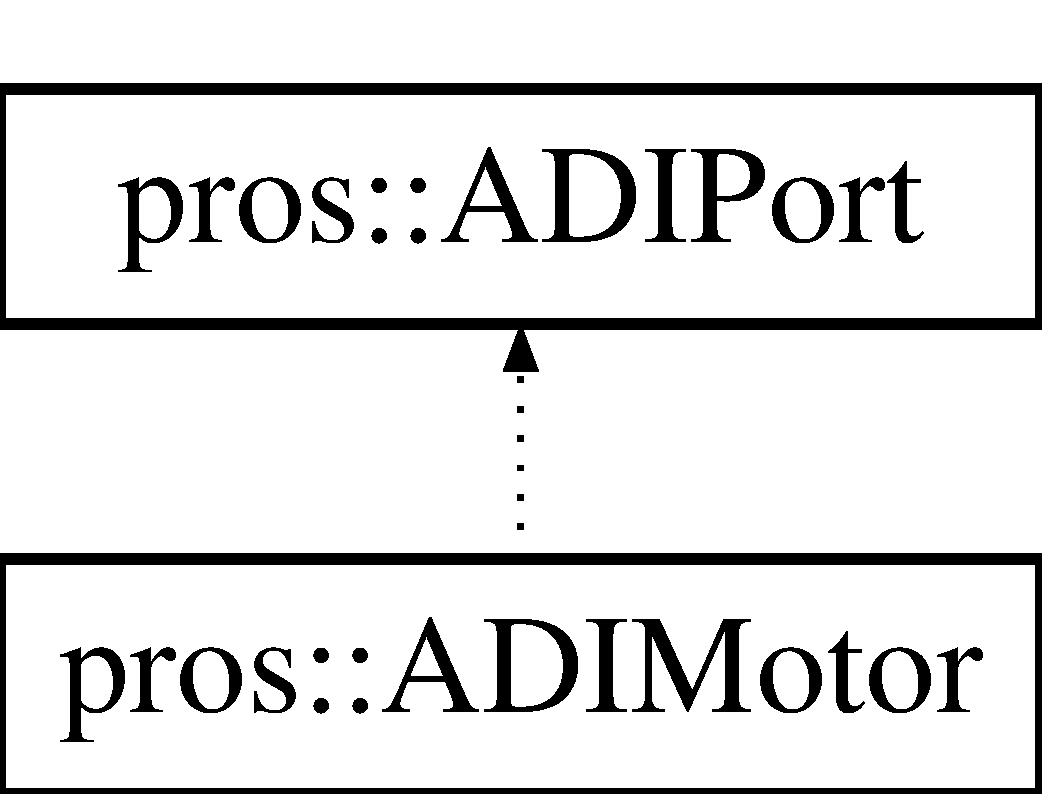
\includegraphics[height=2.000000cm]{classpros_1_1ADIMotor}
\end{center}
\end{figure}
\subsection*{Public Member Functions}
\begin{DoxyCompactItemize}
\item 
\hyperlink{classpros_1_1ADIMotor_afd2da0e8c53a8bc0c999d5232242069a}{A\+D\+I\+Motor} (std\+::uint8\+\_\+t port)
\item 
std\+::int32\+\_\+t \hyperlink{classpros_1_1ADIMotor_ad8e9be8dfbc022e893a4d15996fe3bcd}{stop} (void) const
\end{DoxyCompactItemize}


\subsection{Constructor \& Destructor Documentation}
\mbox{\Hypertarget{classpros_1_1ADIMotor_afd2da0e8c53a8bc0c999d5232242069a}\label{classpros_1_1ADIMotor_afd2da0e8c53a8bc0c999d5232242069a}} 
\index{pros\+::\+A\+D\+I\+Motor@{pros\+::\+A\+D\+I\+Motor}!A\+D\+I\+Motor@{A\+D\+I\+Motor}}
\index{A\+D\+I\+Motor@{A\+D\+I\+Motor}!pros\+::\+A\+D\+I\+Motor@{pros\+::\+A\+D\+I\+Motor}}
\subsubsection{\texorpdfstring{A\+D\+I\+Motor()}{ADIMotor()}}
{\footnotesize\ttfamily pros\+::\+A\+D\+I\+Motor\+::\+A\+D\+I\+Motor (\begin{DoxyParamCaption}\item[{std\+::uint8\+\_\+t}]{port }\end{DoxyParamCaption})}

Configures an A\+DI port to act as a \hyperlink{classpros_1_1Motor}{Motor}.

This function uses the following values of errno when an error state is reached\+: E\+N\+X\+IO -\/ The given value is not within the range of A\+DI Ports.


\begin{DoxyParams}{Parameters}
{\em port} & The A\+DI port number (from 1-\/8, \textquotesingle{}a\textquotesingle{}-\/\textquotesingle{}h\textquotesingle{}, \textquotesingle{}A\textquotesingle{}-\/\textquotesingle{}H\textquotesingle{}) to configure \\
\hline
{\em type} & The configuration type for the port \\
\hline
\end{DoxyParams}


\subsection{Member Function Documentation}
\mbox{\Hypertarget{classpros_1_1ADIMotor_ad8e9be8dfbc022e893a4d15996fe3bcd}\label{classpros_1_1ADIMotor_ad8e9be8dfbc022e893a4d15996fe3bcd}} 
\index{pros\+::\+A\+D\+I\+Motor@{pros\+::\+A\+D\+I\+Motor}!stop@{stop}}
\index{stop@{stop}!pros\+::\+A\+D\+I\+Motor@{pros\+::\+A\+D\+I\+Motor}}
\subsubsection{\texorpdfstring{stop()}{stop()}}
{\footnotesize\ttfamily std\+::int32\+\_\+t pros\+::\+A\+D\+I\+Motor\+::stop (\begin{DoxyParamCaption}\item[{void}]{ }\end{DoxyParamCaption}) const}

Stops the motor on the given port.

This function uses the following values of errno when an error state is reached\+: E\+N\+O\+D\+EV -\/ The port is not configured as a motor

\begin{DoxyReturn}{Returns}
1 if the operation was successful or P\+R\+O\+S\+\_\+\+E\+RR if the operation failed, setting errno. 
\end{DoxyReturn}


The documentation for this class was generated from the following file\+:\begin{DoxyCompactItemize}
\item 
pros/include/pros/\hyperlink{adi_8hpp}{adi.\+hpp}\end{DoxyCompactItemize}

\hypertarget{classpros_1_1ADIPort}{}\section{pros\+:\+:A\+D\+I\+Port Class Reference}
\label{classpros_1_1ADIPort}\index{pros\+::\+A\+D\+I\+Port@{pros\+::\+A\+D\+I\+Port}}


{\ttfamily \#include $<$adi.\+hpp$>$}

Inheritance diagram for pros\+:\+:A\+D\+I\+Port\+:\begin{figure}[H]
\begin{center}
\leavevmode
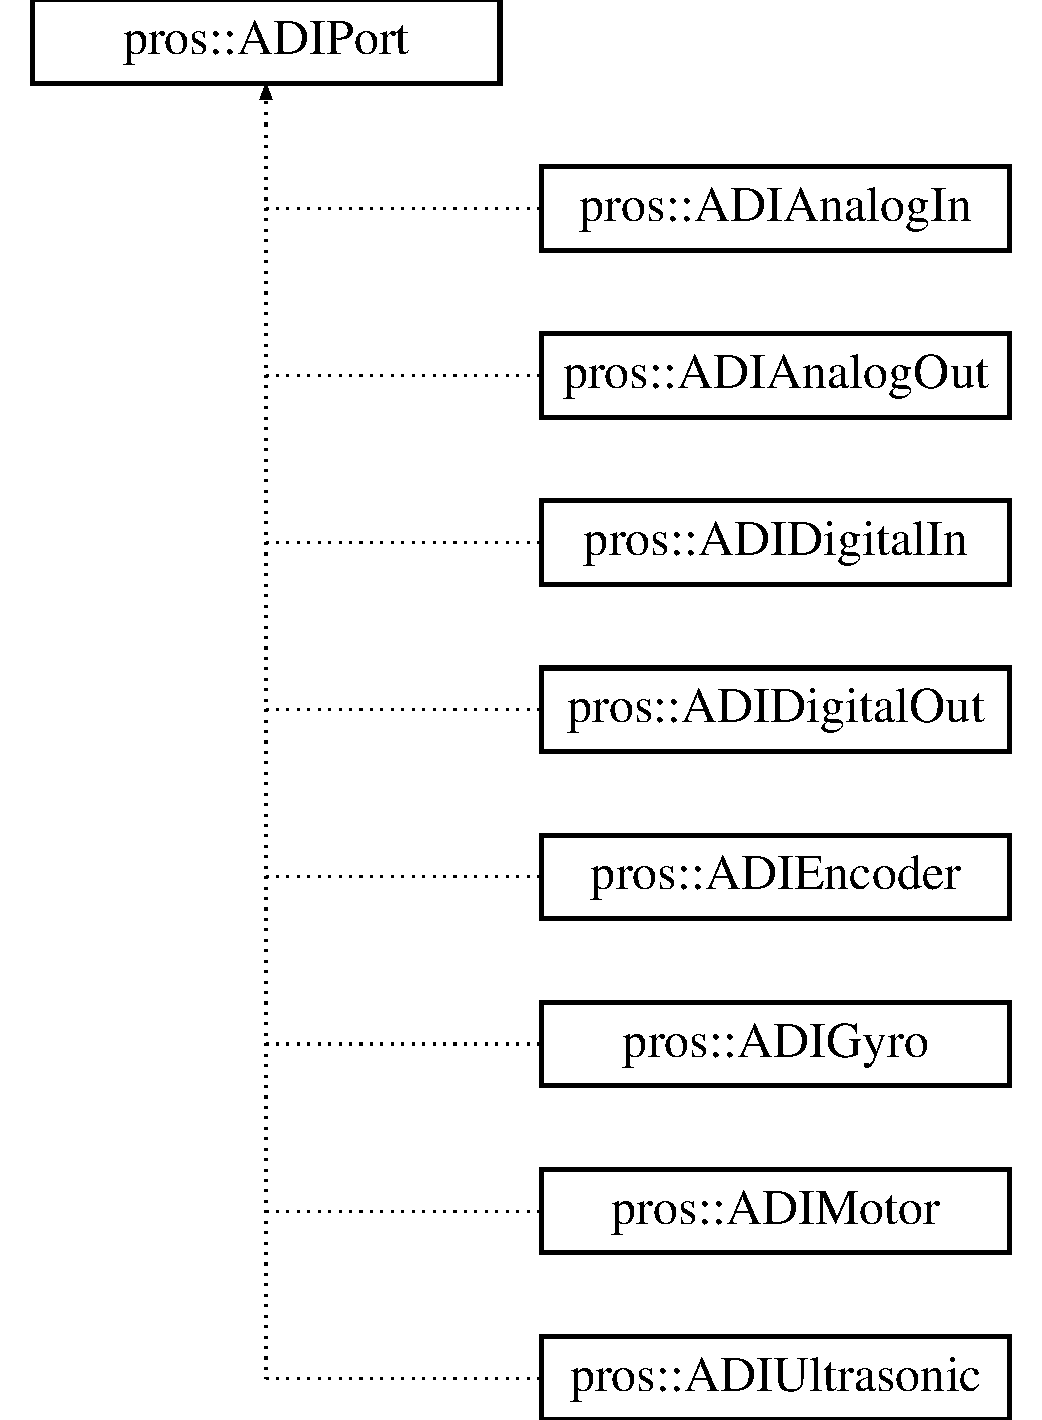
\includegraphics[height=9.000000cm]{classpros_1_1ADIPort}
\end{center}
\end{figure}
\subsection*{Public Member Functions}
\begin{DoxyCompactItemize}
\item 
\hyperlink{classpros_1_1ADIPort_ab6ef7710de366895859d770ffb1d8cf1}{A\+D\+I\+Port} (std\+::uint8\+\_\+t port, \hyperlink{adi_8h_a4efff81399e823764aa05cd5c172ea55}{adi\+\_\+port\+\_\+config\+\_\+e\+\_\+t} type=\hyperlink{adi_8h_ad5f9ddf0fd9de73c4b23fa5485144b7fa37e9d6ebc03d88c58db1904a7f2b7373}{E\+\_\+\+A\+D\+I\+\_\+\+T\+Y\+P\+E\+\_\+\+U\+N\+D\+E\+F\+I\+N\+ED})
\begin{DoxyCompactList}\small\item\em Configures an A\+DI port to act as a given sensor type. \end{DoxyCompactList}\item 
virtual \hyperlink{classpros_1_1ADIPort_ae6a3753c05e008992e6eff5e8c927e46}{$\sim$\+A\+D\+I\+Port} (void)=default
\item 
std\+::int32\+\_\+t \hyperlink{classpros_1_1ADIPort_a1227bc815b12d2789cb78f6d3dcaf37b}{get\+\_\+config} (void) const
\begin{DoxyCompactList}\small\item\em Gets the configuration for the given A\+DI port. \end{DoxyCompactList}\item 
std\+::int32\+\_\+t \hyperlink{classpros_1_1ADIPort_ac79b5fd3ce67ae6ffc4b1fbbb306e997}{get\+\_\+value} (void) const
\begin{DoxyCompactList}\small\item\em Gets the value for the given A\+DI port. \end{DoxyCompactList}\item 
std\+::int32\+\_\+t \hyperlink{classpros_1_1ADIPort_abd86653eebbc34b863ace81839f7e40c}{set\+\_\+config} (\hyperlink{adi_8h_a4efff81399e823764aa05cd5c172ea55}{adi\+\_\+port\+\_\+config\+\_\+e\+\_\+t} type) const
\begin{DoxyCompactList}\small\item\em Configures an A\+DI port to act as a given sensor type. \end{DoxyCompactList}\item 
std\+::int32\+\_\+t \hyperlink{classpros_1_1ADIPort_ae6711117fbceb3bb6e3602c4ef63aff1}{set\+\_\+value} (std\+::int32\+\_\+t value) const
\begin{DoxyCompactList}\small\item\em Sets the value for the given A\+DI port. \end{DoxyCompactList}\end{DoxyCompactItemize}
\subsection*{Protected Member Functions}
\begin{DoxyCompactItemize}
\item 
\hyperlink{classpros_1_1ADIPort_a7f44b44ce0528ea4c5ef83ed8465e72d}{A\+D\+I\+Port} (void)
\end{DoxyCompactItemize}
\subsection*{Protected Attributes}
\begin{DoxyCompactItemize}
\item 
std\+::uint8\+\_\+t \hyperlink{classpros_1_1ADIPort_a75f3b6c1ae3c1f6b755e18444e7559d6}{\+\_\+port}
\end{DoxyCompactItemize}


\subsection{Constructor \& Destructor Documentation}
\mbox{\Hypertarget{classpros_1_1ADIPort_ab6ef7710de366895859d770ffb1d8cf1}\label{classpros_1_1ADIPort_ab6ef7710de366895859d770ffb1d8cf1}} 
\index{pros\+::\+A\+D\+I\+Port@{pros\+::\+A\+D\+I\+Port}!A\+D\+I\+Port@{A\+D\+I\+Port}}
\index{A\+D\+I\+Port@{A\+D\+I\+Port}!pros\+::\+A\+D\+I\+Port@{pros\+::\+A\+D\+I\+Port}}
\subsubsection{\texorpdfstring{A\+D\+I\+Port()}{ADIPort()}\hspace{0.1cm}{\footnotesize\ttfamily [1/2]}}
{\footnotesize\ttfamily pros\+::\+A\+D\+I\+Port\+::\+A\+D\+I\+Port (\begin{DoxyParamCaption}\item[{std\+::uint8\+\_\+t}]{port,  }\item[{\hyperlink{adi_8h_a4efff81399e823764aa05cd5c172ea55}{adi\+\_\+port\+\_\+config\+\_\+e\+\_\+t}}]{type = {\ttfamily \hyperlink{adi_8h_ad5f9ddf0fd9de73c4b23fa5485144b7fa37e9d6ebc03d88c58db1904a7f2b7373}{E\+\_\+\+A\+D\+I\+\_\+\+T\+Y\+P\+E\+\_\+\+U\+N\+D\+E\+F\+I\+N\+ED}} }\end{DoxyParamCaption})}



Configures an A\+DI port to act as a given sensor type. 

This function uses the following values of errno when an error state is reached\+: E\+N\+X\+IO -\/ The given value is not within the range of A\+DI Ports


\begin{DoxyParams}{Parameters}
{\em port} & The A\+DI port number (from 1-\/8, \textquotesingle{}a\textquotesingle{}-\/\textquotesingle{}h\textquotesingle{}, \textquotesingle{}A\textquotesingle{}-\/\textquotesingle{}H\textquotesingle{}) to configure \\
\hline
{\em type} & The configuration type for the port \\
\hline
\end{DoxyParams}
\mbox{\Hypertarget{classpros_1_1ADIPort_ae6a3753c05e008992e6eff5e8c927e46}\label{classpros_1_1ADIPort_ae6a3753c05e008992e6eff5e8c927e46}} 
\index{pros\+::\+A\+D\+I\+Port@{pros\+::\+A\+D\+I\+Port}!````~A\+D\+I\+Port@{$\sim$\+A\+D\+I\+Port}}
\index{````~A\+D\+I\+Port@{$\sim$\+A\+D\+I\+Port}!pros\+::\+A\+D\+I\+Port@{pros\+::\+A\+D\+I\+Port}}
\subsubsection{\texorpdfstring{$\sim$\+A\+D\+I\+Port()}{~ADIPort()}}
{\footnotesize\ttfamily virtual pros\+::\+A\+D\+I\+Port\+::$\sim$\+A\+D\+I\+Port (\begin{DoxyParamCaption}\item[{void}]{ }\end{DoxyParamCaption})\hspace{0.3cm}{\ttfamily [virtual]}, {\ttfamily [default]}}

\mbox{\Hypertarget{classpros_1_1ADIPort_a7f44b44ce0528ea4c5ef83ed8465e72d}\label{classpros_1_1ADIPort_a7f44b44ce0528ea4c5ef83ed8465e72d}} 
\index{pros\+::\+A\+D\+I\+Port@{pros\+::\+A\+D\+I\+Port}!A\+D\+I\+Port@{A\+D\+I\+Port}}
\index{A\+D\+I\+Port@{A\+D\+I\+Port}!pros\+::\+A\+D\+I\+Port@{pros\+::\+A\+D\+I\+Port}}
\subsubsection{\texorpdfstring{A\+D\+I\+Port()}{ADIPort()}\hspace{0.1cm}{\footnotesize\ttfamily [2/2]}}
{\footnotesize\ttfamily pros\+::\+A\+D\+I\+Port\+::\+A\+D\+I\+Port (\begin{DoxyParamCaption}\item[{void}]{ }\end{DoxyParamCaption})\hspace{0.3cm}{\ttfamily [protected]}}



\subsection{Member Function Documentation}
\mbox{\Hypertarget{classpros_1_1ADIPort_a1227bc815b12d2789cb78f6d3dcaf37b}\label{classpros_1_1ADIPort_a1227bc815b12d2789cb78f6d3dcaf37b}} 
\index{pros\+::\+A\+D\+I\+Port@{pros\+::\+A\+D\+I\+Port}!get\+\_\+config@{get\+\_\+config}}
\index{get\+\_\+config@{get\+\_\+config}!pros\+::\+A\+D\+I\+Port@{pros\+::\+A\+D\+I\+Port}}
\subsubsection{\texorpdfstring{get\+\_\+config()}{get\_config()}}
{\footnotesize\ttfamily std\+::int32\+\_\+t pros\+::\+A\+D\+I\+Port\+::get\+\_\+config (\begin{DoxyParamCaption}\item[{void}]{ }\end{DoxyParamCaption}) const}



Gets the configuration for the given A\+DI port. 

\begin{DoxyReturn}{Returns}
The A\+DI configuration for the given port 
\end{DoxyReturn}
\mbox{\Hypertarget{classpros_1_1ADIPort_ac79b5fd3ce67ae6ffc4b1fbbb306e997}\label{classpros_1_1ADIPort_ac79b5fd3ce67ae6ffc4b1fbbb306e997}} 
\index{pros\+::\+A\+D\+I\+Port@{pros\+::\+A\+D\+I\+Port}!get\+\_\+value@{get\+\_\+value}}
\index{get\+\_\+value@{get\+\_\+value}!pros\+::\+A\+D\+I\+Port@{pros\+::\+A\+D\+I\+Port}}
\subsubsection{\texorpdfstring{get\+\_\+value()}{get\_value()}}
{\footnotesize\ttfamily std\+::int32\+\_\+t pros\+::\+A\+D\+I\+Port\+::get\+\_\+value (\begin{DoxyParamCaption}\item[{void}]{ }\end{DoxyParamCaption}) const}



Gets the value for the given A\+DI port. 

\begin{DoxyReturn}{Returns}
The value stored for the given port 
\end{DoxyReturn}
\mbox{\Hypertarget{classpros_1_1ADIPort_abd86653eebbc34b863ace81839f7e40c}\label{classpros_1_1ADIPort_abd86653eebbc34b863ace81839f7e40c}} 
\index{pros\+::\+A\+D\+I\+Port@{pros\+::\+A\+D\+I\+Port}!set\+\_\+config@{set\+\_\+config}}
\index{set\+\_\+config@{set\+\_\+config}!pros\+::\+A\+D\+I\+Port@{pros\+::\+A\+D\+I\+Port}}
\subsubsection{\texorpdfstring{set\+\_\+config()}{set\_config()}}
{\footnotesize\ttfamily std\+::int32\+\_\+t pros\+::\+A\+D\+I\+Port\+::set\+\_\+config (\begin{DoxyParamCaption}\item[{\hyperlink{adi_8h_a4efff81399e823764aa05cd5c172ea55}{adi\+\_\+port\+\_\+config\+\_\+e\+\_\+t}}]{type }\end{DoxyParamCaption}) const}



Configures an A\+DI port to act as a given sensor type. 


\begin{DoxyParams}{Parameters}
{\em type} & The configuration type for the port\\
\hline
\end{DoxyParams}
\begin{DoxyReturn}{Returns}
1 if the operation was successful or P\+R\+O\+S\+\_\+\+E\+RR if the operation failed, setting errno. 
\end{DoxyReturn}
\mbox{\Hypertarget{classpros_1_1ADIPort_ae6711117fbceb3bb6e3602c4ef63aff1}\label{classpros_1_1ADIPort_ae6711117fbceb3bb6e3602c4ef63aff1}} 
\index{pros\+::\+A\+D\+I\+Port@{pros\+::\+A\+D\+I\+Port}!set\+\_\+value@{set\+\_\+value}}
\index{set\+\_\+value@{set\+\_\+value}!pros\+::\+A\+D\+I\+Port@{pros\+::\+A\+D\+I\+Port}}
\subsubsection{\texorpdfstring{set\+\_\+value()}{set\_value()}}
{\footnotesize\ttfamily std\+::int32\+\_\+t pros\+::\+A\+D\+I\+Port\+::set\+\_\+value (\begin{DoxyParamCaption}\item[{std\+::int32\+\_\+t}]{value }\end{DoxyParamCaption}) const}



Sets the value for the given A\+DI port. 

This only works on ports configured as outputs, and the behavior will change depending on the configuration of the port.


\begin{DoxyParams}{Parameters}
{\em value} & The value to set the A\+DI port to\\
\hline
\end{DoxyParams}
\begin{DoxyReturn}{Returns}
1 if the operation was successful or P\+R\+O\+S\+\_\+\+E\+RR if the operation failed, setting errno. 
\end{DoxyReturn}


\subsection{Member Data Documentation}
\mbox{\Hypertarget{classpros_1_1ADIPort_a75f3b6c1ae3c1f6b755e18444e7559d6}\label{classpros_1_1ADIPort_a75f3b6c1ae3c1f6b755e18444e7559d6}} 
\index{pros\+::\+A\+D\+I\+Port@{pros\+::\+A\+D\+I\+Port}!\+\_\+port@{\+\_\+port}}
\index{\+\_\+port@{\+\_\+port}!pros\+::\+A\+D\+I\+Port@{pros\+::\+A\+D\+I\+Port}}
\subsubsection{\texorpdfstring{\+\_\+port}{\_port}}
{\footnotesize\ttfamily std\+::uint8\+\_\+t pros\+::\+A\+D\+I\+Port\+::\+\_\+port\hspace{0.3cm}{\ttfamily [protected]}}



The documentation for this class was generated from the following file\+:\begin{DoxyCompactItemize}
\item 
pros/include/pros/\hyperlink{adi_8hpp}{adi.\+hpp}\end{DoxyCompactItemize}

\hypertarget{classpros_1_1ADIUltrasonic}{}\section{pros\+:\+:A\+D\+I\+Ultrasonic Class Reference}
\label{classpros_1_1ADIUltrasonic}\index{pros\+::\+A\+D\+I\+Ultrasonic@{pros\+::\+A\+D\+I\+Ultrasonic}}


{\ttfamily \#include \char`\"{}adi.\+hpp\char`\"{}}

Inheritance diagram for pros\+:\+:A\+D\+I\+Ultrasonic\+:\begin{figure}[H]
\begin{center}
\leavevmode
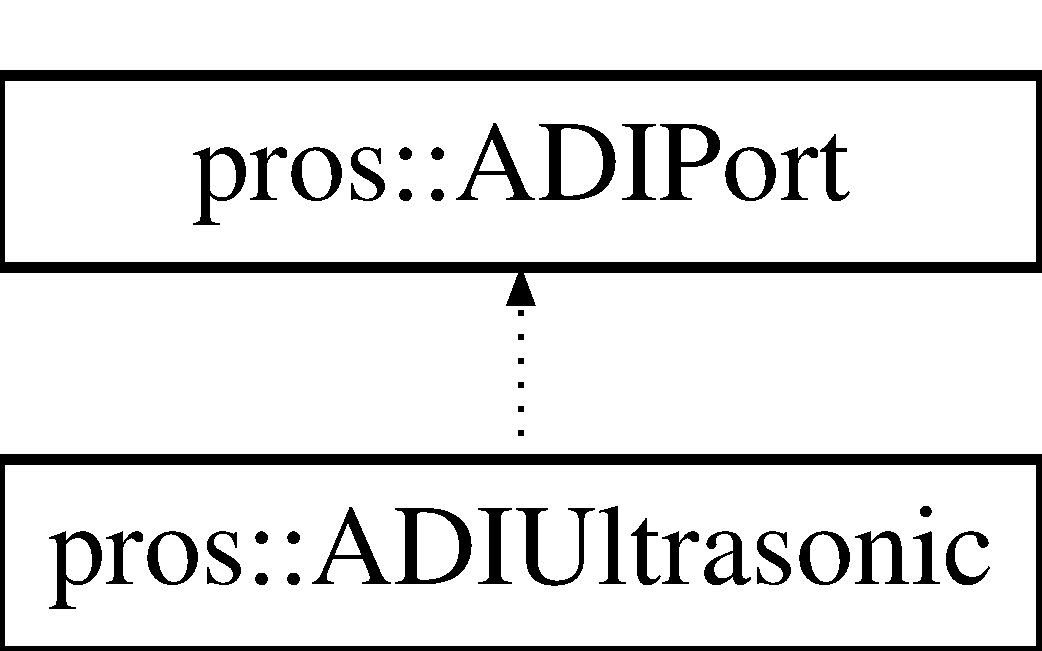
\includegraphics[height=2.000000cm]{classpros_1_1ADIUltrasonic}
\end{center}
\end{figure}
\subsection*{Public Member Functions}
\begin{DoxyCompactItemize}
\item 
\hyperlink{classpros_1_1ADIUltrasonic_ae2b4cd186556af9602cc0017d324494b}{A\+D\+I\+Ultrasonic} (std\+::uint8\+\_\+t port\+\_\+ping, std\+::uint8\+\_\+t port\+\_\+echo)
\begin{DoxyCompactList}\small\item\em Configures a set of A\+DI ports to act as an Ultrasonic. \end{DoxyCompactList}\end{DoxyCompactItemize}


\subsection{Constructor \& Destructor Documentation}
\mbox{\Hypertarget{classpros_1_1ADIUltrasonic_ae2b4cd186556af9602cc0017d324494b}\label{classpros_1_1ADIUltrasonic_ae2b4cd186556af9602cc0017d324494b}} 
\index{pros\+::\+A\+D\+I\+Ultrasonic@{pros\+::\+A\+D\+I\+Ultrasonic}!A\+D\+I\+Ultrasonic@{A\+D\+I\+Ultrasonic}}
\index{A\+D\+I\+Ultrasonic@{A\+D\+I\+Ultrasonic}!pros\+::\+A\+D\+I\+Ultrasonic@{pros\+::\+A\+D\+I\+Ultrasonic}}
\subsubsection{\texorpdfstring{A\+D\+I\+Ultrasonic()}{ADIUltrasonic()}}
{\footnotesize\ttfamily pros\+::\+A\+D\+I\+Ultrasonic\+::\+A\+D\+I\+Ultrasonic (\begin{DoxyParamCaption}\item[{std\+::uint8\+\_\+t}]{port\+\_\+ping,  }\item[{std\+::uint8\+\_\+t}]{port\+\_\+echo }\end{DoxyParamCaption})}



Configures a set of A\+DI ports to act as an Ultrasonic. 

This function uses the following values of errno when an error state is reached\+: E\+N\+X\+IO -\/ The given value is not within the range of A\+DI Ports.


\begin{DoxyParams}{Parameters}
{\em port\+\_\+ping} & The port connected to the orange O\+U\+T\+P\+UT cable. This should be in port 1, 3, 5, or 7 (\textquotesingle{}A\textquotesingle{}, \textquotesingle{}C\textquotesingle{}, \textquotesingle{}E\textquotesingle{}, \textquotesingle{}G\textquotesingle{}). \\
\hline
{\em port\+\_\+echo} & The port connected to the yellow I\+N\+P\+UT cable. This should be in the next highest port following port\+\_\+ping. \\
\hline
\end{DoxyParams}


The documentation for this class was generated from the following file\+:\begin{DoxyCompactItemize}
\item 
pros/include/pros/\hyperlink{adi_8hpp}{adi.\+hpp}\end{DoxyCompactItemize}

\hypertarget{classpros_1_1Controller}{}\section{pros\+:\+:Controller Class Reference}
\label{classpros_1_1Controller}\index{pros\+::\+Controller@{pros\+::\+Controller}}


{\ttfamily \#include $<$misc.\+hpp$>$}

\subsection*{Public Member Functions}
\begin{DoxyCompactItemize}
\item 
\hyperlink{classpros_1_1Controller_ae9d9ead11894048b383e9e82ef46d5ad}{Controller} (\hyperlink{misc_8h_af1323f00203099060d46f722b1fbd460}{controller\+\_\+id\+\_\+e\+\_\+t} id)
\begin{DoxyCompactList}\small\item\em Creates a controller object for the given controller id. \end{DoxyCompactList}\item 
std\+::int32\+\_\+t \hyperlink{classpros_1_1Controller_a1a013e9cf1979487f2daabcd729d3ecb}{is\+\_\+connected} (void)
\begin{DoxyCompactList}\small\item\em Checks if the controller is connected. \end{DoxyCompactList}\item 
std\+::int32\+\_\+t \hyperlink{classpros_1_1Controller_ace3038684aa3cf14f06279c54eeb1105}{get\+\_\+analog} (\hyperlink{misc_8h_a8bdd0963e2bc0d4fbe03435eee8a5ca5}{controller\+\_\+analog\+\_\+e\+\_\+t} channel)
\begin{DoxyCompactList}\small\item\em Gets the value of an analog channel (joystick) on a controller. \end{DoxyCompactList}\item 
std\+::int32\+\_\+t \hyperlink{classpros_1_1Controller_a7d85ecacfd46161ddb2be08d856ca130}{get\+\_\+battery\+\_\+capacity} (void)
\begin{DoxyCompactList}\small\item\em Gets the battery capacity of the controller. \end{DoxyCompactList}\item 
std\+::int32\+\_\+t \hyperlink{classpros_1_1Controller_a8fd8b131f13f2f7702b5299dab82fdaf}{get\+\_\+battery\+\_\+level} (void)
\begin{DoxyCompactList}\small\item\em Gets the battery level of the controller. \end{DoxyCompactList}\item 
std\+::int32\+\_\+t \hyperlink{classpros_1_1Controller_aec180b0f1700915007de2b7855070c80}{get\+\_\+digital} (\hyperlink{misc_8h_a8c380ff02828ee53954bc0ce274253ed}{controller\+\_\+digital\+\_\+e\+\_\+t} button)
\begin{DoxyCompactList}\small\item\em Checks if a digital channel (button) on the controller is currently pressed. \end{DoxyCompactList}\item 
std\+::int32\+\_\+t \hyperlink{classpros_1_1Controller_a9dc7dc6028431d3f8f9aff0fc7a4bed6}{get\+\_\+digital\+\_\+new\+\_\+press} (\hyperlink{misc_8h_a8c380ff02828ee53954bc0ce274253ed}{controller\+\_\+digital\+\_\+e\+\_\+t} button)
\begin{DoxyCompactList}\small\item\em Returns a rising-\/edge case for a controller button press. \end{DoxyCompactList}\item 
{\footnotesize template$<$typename T $>$ }\\T \hyperlink{classpros_1_1Controller_ae0a289e9e55e8f861591af1a6407a0f8}{convert\+\_\+args} (T arg)
\item 
const char $\ast$ \hyperlink{classpros_1_1Controller_a80ab1bf077cfe15fa9b7c4cba27428ef}{convert\+\_\+args} (const std\+::string \&arg)
\item 
{\footnotesize template$<$typename... Params$>$ }\\std\+::int32\+\_\+t \hyperlink{classpros_1_1Controller_a4a301df3d34578661271f9b400da1176}{print} (std\+::uint8\+\_\+t line, std\+::uint8\+\_\+t col, const char $\ast$fmt, Params... args)
\begin{DoxyCompactList}\small\item\em Sets text to the controller L\+CD screen. \end{DoxyCompactList}\item 
std\+::int32\+\_\+t \hyperlink{classpros_1_1Controller_a2ec84a072d09a4bb39253956662604cd}{set\+\_\+text} (std\+::uint8\+\_\+t line, std\+::uint8\+\_\+t col, const char $\ast$str)
\begin{DoxyCompactList}\small\item\em Sets text to the controller L\+CD screen. \end{DoxyCompactList}\item 
std\+::int32\+\_\+t \hyperlink{classpros_1_1Controller_a9f65f6c26d55619a658aa103d3532583}{clear\+\_\+line} (std\+::uint8\+\_\+t line)
\begin{DoxyCompactList}\small\item\em Clears an individual line of the controller screen. \end{DoxyCompactList}\item 
std\+::int32\+\_\+t \hyperlink{classpros_1_1Controller_ac2436bc570bdce79da5954eb895fd234}{rumble} (const char $\ast$rumble\+\_\+pattern)
\begin{DoxyCompactList}\small\item\em Rumble the controller. \end{DoxyCompactList}\item 
std\+::int32\+\_\+t \hyperlink{classpros_1_1Controller_a49a332fe032c3aaf94e24bb3a51945e1}{clear} (void)
\begin{DoxyCompactList}\small\item\em Clears all of the lines on the controller screen. \end{DoxyCompactList}\end{DoxyCompactItemize}


\subsection{Constructor \& Destructor Documentation}
\mbox{\Hypertarget{classpros_1_1Controller_ae9d9ead11894048b383e9e82ef46d5ad}\label{classpros_1_1Controller_ae9d9ead11894048b383e9e82ef46d5ad}} 
\index{pros\+::\+Controller@{pros\+::\+Controller}!Controller@{Controller}}
\index{Controller@{Controller}!pros\+::\+Controller@{pros\+::\+Controller}}
\subsubsection{\texorpdfstring{Controller()}{Controller()}}
{\footnotesize\ttfamily pros\+::\+Controller\+::\+Controller (\begin{DoxyParamCaption}\item[{\hyperlink{misc_8h_af1323f00203099060d46f722b1fbd460}{controller\+\_\+id\+\_\+e\+\_\+t}}]{id }\end{DoxyParamCaption})}



Creates a controller object for the given controller id. 


\begin{DoxyParams}{Parameters}
{\em id} & The ID of the controller (e.\+g. the master or partner controller). Must be one of C\+O\+N\+T\+R\+O\+L\+L\+E\+R\+\_\+\+M\+A\+S\+T\+ER or C\+O\+N\+T\+R\+O\+L\+L\+E\+R\+\_\+\+P\+A\+R\+T\+N\+ER \\
\hline
\end{DoxyParams}


\subsection{Member Function Documentation}
\mbox{\Hypertarget{classpros_1_1Controller_a49a332fe032c3aaf94e24bb3a51945e1}\label{classpros_1_1Controller_a49a332fe032c3aaf94e24bb3a51945e1}} 
\index{pros\+::\+Controller@{pros\+::\+Controller}!clear@{clear}}
\index{clear@{clear}!pros\+::\+Controller@{pros\+::\+Controller}}
\subsubsection{\texorpdfstring{clear()}{clear()}}
{\footnotesize\ttfamily std\+::int32\+\_\+t pros\+::\+Controller\+::clear (\begin{DoxyParamCaption}\item[{void}]{ }\end{DoxyParamCaption})}



Clears all of the lines on the controller screen. 

\begin{DoxyNote}{Note}
\hyperlink{classpros_1_1Controller}{Controller} text setting is currently in beta, so continuous, fast updates will not work well. On vex\+OS version 1.\+0.\+0 this function will block for 110ms.
\end{DoxyNote}
This function uses the following values of errno when an error state is reached\+: E\+A\+C\+C\+ES -\/ Another resource is currently trying to access the controller port.

\begin{DoxyReturn}{Returns}
1 if the operation was successful or P\+R\+O\+S\+\_\+\+E\+RR if the operation failed, setting errno. 
\end{DoxyReturn}
\mbox{\Hypertarget{classpros_1_1Controller_a9f65f6c26d55619a658aa103d3532583}\label{classpros_1_1Controller_a9f65f6c26d55619a658aa103d3532583}} 
\index{pros\+::\+Controller@{pros\+::\+Controller}!clear\+\_\+line@{clear\+\_\+line}}
\index{clear\+\_\+line@{clear\+\_\+line}!pros\+::\+Controller@{pros\+::\+Controller}}
\subsubsection{\texorpdfstring{clear\+\_\+line()}{clear\_line()}}
{\footnotesize\ttfamily std\+::int32\+\_\+t pros\+::\+Controller\+::clear\+\_\+line (\begin{DoxyParamCaption}\item[{std\+::uint8\+\_\+t}]{line }\end{DoxyParamCaption})}



Clears an individual line of the controller screen. 

\begin{DoxyNote}{Note}
\hyperlink{classpros_1_1Controller}{Controller} text setting is currently in beta, so continuous, fast updates will not work well.
\end{DoxyNote}
This function uses the following values of errno when an error state is reached\+: E\+A\+C\+C\+ES -\/ Another resource is currently trying to access the controller port.


\begin{DoxyParams}{Parameters}
{\em line} & The line number to clear \mbox{[}0-\/2\mbox{]}\\
\hline
\end{DoxyParams}
\begin{DoxyReturn}{Returns}
1 if the operation was successful or P\+R\+O\+S\+\_\+\+E\+RR if the operation failed, setting errno. 
\end{DoxyReturn}
\mbox{\Hypertarget{classpros_1_1Controller_ae0a289e9e55e8f861591af1a6407a0f8}\label{classpros_1_1Controller_ae0a289e9e55e8f861591af1a6407a0f8}} 
\index{pros\+::\+Controller@{pros\+::\+Controller}!convert\+\_\+args@{convert\+\_\+args}}
\index{convert\+\_\+args@{convert\+\_\+args}!pros\+::\+Controller@{pros\+::\+Controller}}
\subsubsection{\texorpdfstring{convert\+\_\+args()}{convert\_args()}\hspace{0.1cm}{\footnotesize\ttfamily [1/2]}}
{\footnotesize\ttfamily template$<$typename T $>$ \\
T pros\+::\+Controller\+::convert\+\_\+args (\begin{DoxyParamCaption}\item[{T}]{arg }\end{DoxyParamCaption})\hspace{0.3cm}{\ttfamily [inline]}}

\mbox{\Hypertarget{classpros_1_1Controller_a80ab1bf077cfe15fa9b7c4cba27428ef}\label{classpros_1_1Controller_a80ab1bf077cfe15fa9b7c4cba27428ef}} 
\index{pros\+::\+Controller@{pros\+::\+Controller}!convert\+\_\+args@{convert\+\_\+args}}
\index{convert\+\_\+args@{convert\+\_\+args}!pros\+::\+Controller@{pros\+::\+Controller}}
\subsubsection{\texorpdfstring{convert\+\_\+args()}{convert\_args()}\hspace{0.1cm}{\footnotesize\ttfamily [2/2]}}
{\footnotesize\ttfamily const char$\ast$ pros\+::\+Controller\+::convert\+\_\+args (\begin{DoxyParamCaption}\item[{const std\+::string \&}]{arg }\end{DoxyParamCaption})\hspace{0.3cm}{\ttfamily [inline]}}

\mbox{\Hypertarget{classpros_1_1Controller_ace3038684aa3cf14f06279c54eeb1105}\label{classpros_1_1Controller_ace3038684aa3cf14f06279c54eeb1105}} 
\index{pros\+::\+Controller@{pros\+::\+Controller}!get\+\_\+analog@{get\+\_\+analog}}
\index{get\+\_\+analog@{get\+\_\+analog}!pros\+::\+Controller@{pros\+::\+Controller}}
\subsubsection{\texorpdfstring{get\+\_\+analog()}{get\_analog()}}
{\footnotesize\ttfamily std\+::int32\+\_\+t pros\+::\+Controller\+::get\+\_\+analog (\begin{DoxyParamCaption}\item[{\hyperlink{misc_8h_a8bdd0963e2bc0d4fbe03435eee8a5ca5}{controller\+\_\+analog\+\_\+e\+\_\+t}}]{channel }\end{DoxyParamCaption})}



Gets the value of an analog channel (joystick) on a controller. 

This function uses the following values of errno when an error state is reached\+: E\+A\+C\+C\+ES -\/ Another resource is currently trying to access the controller port.


\begin{DoxyParams}{Parameters}
{\em channel} & The analog channel to get. Must be one of A\+N\+A\+L\+O\+G\+\_\+\+L\+E\+F\+T\+\_\+X, A\+N\+A\+L\+O\+G\+\_\+\+L\+E\+F\+T\+\_\+Y, A\+N\+A\+L\+O\+G\+\_\+\+R\+I\+G\+H\+T\+\_\+X, A\+N\+A\+L\+O\+G\+\_\+\+R\+I\+G\+H\+T\+\_\+Y\\
\hline
\end{DoxyParams}
\begin{DoxyReturn}{Returns}
The current reading of the analog channel\+: \mbox{[}-\/127, 127\mbox{]}. If the controller was not connected, then 0 is returned 
\end{DoxyReturn}
\mbox{\Hypertarget{classpros_1_1Controller_a7d85ecacfd46161ddb2be08d856ca130}\label{classpros_1_1Controller_a7d85ecacfd46161ddb2be08d856ca130}} 
\index{pros\+::\+Controller@{pros\+::\+Controller}!get\+\_\+battery\+\_\+capacity@{get\+\_\+battery\+\_\+capacity}}
\index{get\+\_\+battery\+\_\+capacity@{get\+\_\+battery\+\_\+capacity}!pros\+::\+Controller@{pros\+::\+Controller}}
\subsubsection{\texorpdfstring{get\+\_\+battery\+\_\+capacity()}{get\_battery\_capacity()}}
{\footnotesize\ttfamily std\+::int32\+\_\+t pros\+::\+Controller\+::get\+\_\+battery\+\_\+capacity (\begin{DoxyParamCaption}\item[{void}]{ }\end{DoxyParamCaption})}



Gets the battery capacity of the controller. 

This function uses the following values of errno when an error state is reached\+: E\+A\+C\+C\+ES -\/ Another resource is currently trying to access the controller port.

\begin{DoxyReturn}{Returns}
The controller\textquotesingle{}s battery capacity 
\end{DoxyReturn}
\mbox{\Hypertarget{classpros_1_1Controller_a8fd8b131f13f2f7702b5299dab82fdaf}\label{classpros_1_1Controller_a8fd8b131f13f2f7702b5299dab82fdaf}} 
\index{pros\+::\+Controller@{pros\+::\+Controller}!get\+\_\+battery\+\_\+level@{get\+\_\+battery\+\_\+level}}
\index{get\+\_\+battery\+\_\+level@{get\+\_\+battery\+\_\+level}!pros\+::\+Controller@{pros\+::\+Controller}}
\subsubsection{\texorpdfstring{get\+\_\+battery\+\_\+level()}{get\_battery\_level()}}
{\footnotesize\ttfamily std\+::int32\+\_\+t pros\+::\+Controller\+::get\+\_\+battery\+\_\+level (\begin{DoxyParamCaption}\item[{void}]{ }\end{DoxyParamCaption})}



Gets the battery level of the controller. 

This function uses the following values of errno when an error state is reached\+: E\+A\+C\+C\+ES -\/ Another resource is currently trying to access the controller port.

\begin{DoxyReturn}{Returns}
The controller\textquotesingle{}s battery level 
\end{DoxyReturn}
\mbox{\Hypertarget{classpros_1_1Controller_aec180b0f1700915007de2b7855070c80}\label{classpros_1_1Controller_aec180b0f1700915007de2b7855070c80}} 
\index{pros\+::\+Controller@{pros\+::\+Controller}!get\+\_\+digital@{get\+\_\+digital}}
\index{get\+\_\+digital@{get\+\_\+digital}!pros\+::\+Controller@{pros\+::\+Controller}}
\subsubsection{\texorpdfstring{get\+\_\+digital()}{get\_digital()}}
{\footnotesize\ttfamily std\+::int32\+\_\+t pros\+::\+Controller\+::get\+\_\+digital (\begin{DoxyParamCaption}\item[{\hyperlink{misc_8h_a8c380ff02828ee53954bc0ce274253ed}{controller\+\_\+digital\+\_\+e\+\_\+t}}]{button }\end{DoxyParamCaption})}



Checks if a digital channel (button) on the controller is currently pressed. 

This function uses the following values of errno when an error state is reached\+: E\+A\+C\+C\+ES -\/ Another resource is currently trying to access the controller port.


\begin{DoxyParams}{Parameters}
{\em button} & The button to read. Must be one of D\+I\+G\+I\+T\+A\+L\+\_\+\{R\+I\+G\+HT,D\+O\+WN,L\+E\+FT,UP,A,B,Y,X,R1,R2,L1,L2\}\\
\hline
\end{DoxyParams}
\begin{DoxyReturn}{Returns}
1 if the button on the controller is pressed. If the controller was not connected, then 0 is returned 
\end{DoxyReturn}
\mbox{\Hypertarget{classpros_1_1Controller_a9dc7dc6028431d3f8f9aff0fc7a4bed6}\label{classpros_1_1Controller_a9dc7dc6028431d3f8f9aff0fc7a4bed6}} 
\index{pros\+::\+Controller@{pros\+::\+Controller}!get\+\_\+digital\+\_\+new\+\_\+press@{get\+\_\+digital\+\_\+new\+\_\+press}}
\index{get\+\_\+digital\+\_\+new\+\_\+press@{get\+\_\+digital\+\_\+new\+\_\+press}!pros\+::\+Controller@{pros\+::\+Controller}}
\subsubsection{\texorpdfstring{get\+\_\+digital\+\_\+new\+\_\+press()}{get\_digital\_new\_press()}}
{\footnotesize\ttfamily std\+::int32\+\_\+t pros\+::\+Controller\+::get\+\_\+digital\+\_\+new\+\_\+press (\begin{DoxyParamCaption}\item[{\hyperlink{misc_8h_a8c380ff02828ee53954bc0ce274253ed}{controller\+\_\+digital\+\_\+e\+\_\+t}}]{button }\end{DoxyParamCaption})}



Returns a rising-\/edge case for a controller button press. 

This function is not thread-\/safe. Multiple tasks polling a single button may return different results under the same circumstances, so only one task should call this function for any given button. E.\+g., \hyperlink{classpros_1_1Task}{Task} A calls this function for buttons 1 and 2. \hyperlink{classpros_1_1Task}{Task} B may call this function for button 3, but should not for buttons 1 or 2. A typical use-\/case for this function is to call inside opcontrol to detect new button presses, and not in any other tasks.

This function uses the following values of errno when an error state is reached\+: E\+A\+C\+C\+ES -\/ Another resource is currently trying to access the controller port.


\begin{DoxyParams}{Parameters}
{\em button} & The button to read. Must be one of D\+I\+G\+I\+T\+A\+L\+\_\+\{R\+I\+G\+HT,D\+O\+WN,L\+E\+FT,UP,A,B,Y,X,R1,R2,L1,L2\}\\
\hline
\end{DoxyParams}
\begin{DoxyReturn}{Returns}
1 if the button on the controller is pressed and had not been pressed the last time this function was called, 0 otherwise. 
\end{DoxyReturn}
\mbox{\Hypertarget{classpros_1_1Controller_a1a013e9cf1979487f2daabcd729d3ecb}\label{classpros_1_1Controller_a1a013e9cf1979487f2daabcd729d3ecb}} 
\index{pros\+::\+Controller@{pros\+::\+Controller}!is\+\_\+connected@{is\+\_\+connected}}
\index{is\+\_\+connected@{is\+\_\+connected}!pros\+::\+Controller@{pros\+::\+Controller}}
\subsubsection{\texorpdfstring{is\+\_\+connected()}{is\_connected()}}
{\footnotesize\ttfamily std\+::int32\+\_\+t pros\+::\+Controller\+::is\+\_\+connected (\begin{DoxyParamCaption}\item[{void}]{ }\end{DoxyParamCaption})}



Checks if the controller is connected. 

This function uses the following values of errno when an error state is reached\+: E\+A\+C\+C\+ES -\/ Another resource is currently trying to access the controller port.

\begin{DoxyReturn}{Returns}
1 if the controller is connected, 0 otherwise 
\end{DoxyReturn}
\mbox{\Hypertarget{classpros_1_1Controller_a4a301df3d34578661271f9b400da1176}\label{classpros_1_1Controller_a4a301df3d34578661271f9b400da1176}} 
\index{pros\+::\+Controller@{pros\+::\+Controller}!print@{print}}
\index{print@{print}!pros\+::\+Controller@{pros\+::\+Controller}}
\subsubsection{\texorpdfstring{print()}{print()}}
{\footnotesize\ttfamily template$<$typename... Params$>$ \\
std\+::int32\+\_\+t pros\+::\+Controller\+::print (\begin{DoxyParamCaption}\item[{std\+::uint8\+\_\+t}]{line,  }\item[{std\+::uint8\+\_\+t}]{col,  }\item[{const char $\ast$}]{fmt,  }\item[{Params...}]{args }\end{DoxyParamCaption})\hspace{0.3cm}{\ttfamily [inline]}}



Sets text to the controller L\+CD screen. 

\begin{DoxyNote}{Note}
\hyperlink{classpros_1_1Controller}{Controller} text setting is currently in beta, so continuous, fast updates will not work well.
\end{DoxyNote}
This function uses the following values of errno when an error state is reached\+: E\+A\+C\+C\+ES -\/ Another resource is currently trying to access the controller port.


\begin{DoxyParams}{Parameters}
{\em line} & The line number at which the text will be displayed \mbox{[}0-\/2\mbox{]} \\
\hline
{\em col} & The column number at which the text will be displayed \mbox{[}0-\/14\mbox{]} \\
\hline
{\em fmt} & The format string to print to the controller \\
\hline
{\em ...} & The argument list for the format string\\
\hline
\end{DoxyParams}
\begin{DoxyReturn}{Returns}
1 if the operation was successful or P\+R\+O\+S\+\_\+\+E\+RR if the operation failed, setting errno. 
\end{DoxyReturn}
\mbox{\Hypertarget{classpros_1_1Controller_ac2436bc570bdce79da5954eb895fd234}\label{classpros_1_1Controller_ac2436bc570bdce79da5954eb895fd234}} 
\index{pros\+::\+Controller@{pros\+::\+Controller}!rumble@{rumble}}
\index{rumble@{rumble}!pros\+::\+Controller@{pros\+::\+Controller}}
\subsubsection{\texorpdfstring{rumble()}{rumble()}}
{\footnotesize\ttfamily std\+::int32\+\_\+t pros\+::\+Controller\+::rumble (\begin{DoxyParamCaption}\item[{const char $\ast$}]{rumble\+\_\+pattern }\end{DoxyParamCaption})}



Rumble the controller. 

\begin{DoxyNote}{Note}
\hyperlink{classpros_1_1Controller}{Controller} rumble activation is currently in beta, so continuous, fast updates will not work well.
\end{DoxyNote}
This function uses the following values of errno when an error state is reached\+: E\+A\+C\+C\+ES -\/ Another resource is currently trying to access the controller port.


\begin{DoxyParams}{Parameters}
{\em rumble\+\_\+pattern} & A string consisting of the characters \textquotesingle{}.\textquotesingle{}, \textquotesingle{}-\/\textquotesingle{}, and \textquotesingle{} \textquotesingle{}, where dots are short rumbles, dashes are long rumbles, and spaces are pauses. Maximum supported length is 8 characters.\\
\hline
\end{DoxyParams}
\begin{DoxyReturn}{Returns}
1 if the operation was successful or P\+R\+O\+S\+\_\+\+E\+RR if the operation failed, setting errno. 
\end{DoxyReturn}
\mbox{\Hypertarget{classpros_1_1Controller_a2ec84a072d09a4bb39253956662604cd}\label{classpros_1_1Controller_a2ec84a072d09a4bb39253956662604cd}} 
\index{pros\+::\+Controller@{pros\+::\+Controller}!set\+\_\+text@{set\+\_\+text}}
\index{set\+\_\+text@{set\+\_\+text}!pros\+::\+Controller@{pros\+::\+Controller}}
\subsubsection{\texorpdfstring{set\+\_\+text()}{set\_text()}}
{\footnotesize\ttfamily std\+::int32\+\_\+t pros\+::\+Controller\+::set\+\_\+text (\begin{DoxyParamCaption}\item[{std\+::uint8\+\_\+t}]{line,  }\item[{std\+::uint8\+\_\+t}]{col,  }\item[{const char $\ast$}]{str }\end{DoxyParamCaption})}



Sets text to the controller L\+CD screen. 

\begin{DoxyNote}{Note}
\hyperlink{classpros_1_1Controller}{Controller} text setting is currently in beta, so continuous, fast updates will not work well.
\end{DoxyNote}
This function uses the following values of errno when an error state is reached\+: E\+A\+C\+C\+ES -\/ Another resource is currently trying to access the controller port.


\begin{DoxyParams}{Parameters}
{\em line} & The line number at which the text will be displayed \mbox{[}0-\/2\mbox{]} \\
\hline
{\em col} & The column number at which the text will be displayed \mbox{[}0-\/14\mbox{]} \\
\hline
{\em str} & The pre-\/formatted string to print to the controller\\
\hline
\end{DoxyParams}
\begin{DoxyReturn}{Returns}
1 if the operation was successful or P\+R\+O\+S\+\_\+\+E\+RR if the operation failed, setting errno. 
\end{DoxyReturn}


The documentation for this class was generated from the following file\+:\begin{DoxyCompactItemize}
\item 
pros/include/pros/\hyperlink{misc_8hpp}{misc.\+hpp}\end{DoxyCompactItemize}

\hypertarget{classpros_1_1Imu}{}\doxysection{Imu Class Reference}
\label{classpros_1_1Imu}\index{Imu@{Imu}}


{\ttfamily \#include \char`\"{}imu.\+hpp\char`\"{}}

\doxysubsection*{Public Member Functions}
\begin{DoxyCompactItemize}
\item 
\mbox{\hyperlink{classpros_1_1Imu_ac6f1a6d4484080397cb0c78eabea166b}{Imu}} (const std\+::uint8\+\_\+t port)
\item 
virtual std\+::int32\+\_\+t \mbox{\hyperlink{classpros_1_1Imu_a0e653310bbf7ecde3d2f58b019731a98}{reset}} () const
\begin{DoxyCompactList}\small\item\em Calibrate I\+MU. \end{DoxyCompactList}\item 
virtual double \mbox{\hyperlink{classpros_1_1Imu_a60630447c3ada8da63dd91e092eeb2fd}{get\+\_\+rotation}} () const
\begin{DoxyCompactList}\small\item\em Get the total number of degrees the Inertial Sensor has spun about the z-\/axis. \end{DoxyCompactList}\item 
virtual double \mbox{\hyperlink{classpros_1_1Imu_a16a339b5f7729298dc79cf4971565043}{get\+\_\+heading}} () const
\begin{DoxyCompactList}\small\item\em Get the Inertial Sensor\textquotesingle{}s heading relative to the initial direction of its x-\/axis. \end{DoxyCompactList}\item 
virtual \mbox{\hyperlink{namespacepros_1_1c_a1f3d4bf4251e6ce7cb374297de6390a1}{pros\+::c\+::quaternion\+\_\+s\+\_\+t}} \mbox{\hyperlink{classpros_1_1Imu_a85c2835f1335fa5cab843d3bf98cfa15}{get\+\_\+quaternion}} () const
\begin{DoxyCompactList}\small\item\em Get a quaternion representing the Inertial Sensor\textquotesingle{}s orientation. \end{DoxyCompactList}\item 
virtual \mbox{\hyperlink{namespacepros_1_1c_a93e80020ec907b7e11ac7166e5d01c55}{pros\+::c\+::euler\+\_\+s\+\_\+t}} \mbox{\hyperlink{classpros_1_1Imu_a6776d4363caafc3eaa79e638e80ef2ef}{get\+\_\+euler}} () const
\begin{DoxyCompactList}\small\item\em Get the Euler angles representing the Inertial Sensor\textquotesingle{}s orientation. \end{DoxyCompactList}\item 
virtual double \mbox{\hyperlink{classpros_1_1Imu_a74b63ffbb1f1a31e6f1bb740b8c4f823}{get\+\_\+pitch}} () const
\begin{DoxyCompactList}\small\item\em Get the Inertial Sensor\textquotesingle{}s pitch angle. \end{DoxyCompactList}\item 
virtual double \mbox{\hyperlink{classpros_1_1Imu_a25b06e3629127c64370d43454b04696f}{get\+\_\+roll}} () const
\begin{DoxyCompactList}\small\item\em Get the Inertial Sensor\textquotesingle{}s roll angle. \end{DoxyCompactList}\item 
virtual double \mbox{\hyperlink{classpros_1_1Imu_a757ff3f4ff5e6646db7a158bdc951dc2}{get\+\_\+yaw}} () const
\begin{DoxyCompactList}\small\item\em Get the Inertial Sensor\textquotesingle{}s yaw angle. \end{DoxyCompactList}\item 
virtual \mbox{\hyperlink{namespacepros_1_1c_a5b9e240cfb181cce3c741e29efbbbf23}{pros\+::c\+::imu\+\_\+gyro\+\_\+s\+\_\+t}} \mbox{\hyperlink{classpros_1_1Imu_aaaa0cfbbaa188bbbf2813dfbfa3df251}{get\+\_\+gyro\+\_\+rate}} () const
\begin{DoxyCompactList}\small\item\em Get the Inertial Sensor\textquotesingle{}s raw gyroscope values. \end{DoxyCompactList}\item 
virtual \mbox{\hyperlink{namespacepros_1_1c_a70eb3173193f4f46266eade4c243f662}{pros\+::c\+::imu\+\_\+accel\+\_\+s\+\_\+t}} \mbox{\hyperlink{classpros_1_1Imu_a0873891d9b40c12e3c7715fd033a6658}{get\+\_\+accel}} () const
\begin{DoxyCompactList}\small\item\em Get the Inertial Sensor\textquotesingle{}s raw acceleroneter values. \end{DoxyCompactList}\item 
virtual pros\+::c\+::imu\+\_\+status\+\_\+e\+\_\+t \mbox{\hyperlink{classpros_1_1Imu_af5c4fe4981b56fa1e4ae1cc1c2e29d76}{get\+\_\+status}} () const
\begin{DoxyCompactList}\small\item\em Get the Inertial Sensor\textquotesingle{}s status. \end{DoxyCompactList}\item 
virtual bool \mbox{\hyperlink{classpros_1_1Imu_ac58cd647360441bf82830bd17d2f6c82}{is\+\_\+calibrating}} () const
\begin{DoxyCompactList}\small\item\em Check whether the I\+MU is calibrating. \end{DoxyCompactList}\end{DoxyCompactItemize}


\doxysubsection{Constructor \& Destructor Documentation}
\mbox{\Hypertarget{classpros_1_1Imu_ac6f1a6d4484080397cb0c78eabea166b}\label{classpros_1_1Imu_ac6f1a6d4484080397cb0c78eabea166b}} 
\index{Imu@{Imu}!Imu@{Imu}}
\index{Imu@{Imu}!Imu@{Imu}}
\doxysubsubsection{\texorpdfstring{Imu()}{Imu()}}
{\footnotesize\ttfamily \mbox{\hyperlink{classpros_1_1Imu}{Imu}} (\begin{DoxyParamCaption}\item[{const std\+::uint8\+\_\+t}]{port }\end{DoxyParamCaption})\hspace{0.3cm}{\ttfamily [inline]}}



\doxysubsection{Member Function Documentation}
\mbox{\Hypertarget{classpros_1_1Imu_a0e653310bbf7ecde3d2f58b019731a98}\label{classpros_1_1Imu_a0e653310bbf7ecde3d2f58b019731a98}} 
\index{Imu@{Imu}!reset@{reset}}
\index{reset@{reset}!Imu@{Imu}}
\doxysubsubsection{\texorpdfstring{reset()}{reset()}}
{\footnotesize\ttfamily virtual std\+::int32\+\_\+t reset (\begin{DoxyParamCaption}{ }\end{DoxyParamCaption}) const\hspace{0.3cm}{\ttfamily [virtual]}}



Calibrate I\+MU. 

This takes approximately 2 seconds, and is a non-\/blocking operation.

This function uses the following values of errno when an error state is reached\+: E\+N\+X\+IO -\/ The given value is not within the range of V5 ports (1-\/21). E\+N\+O\+D\+EV -\/ The port cannot be configured as an Inertial Sensor E\+A\+G\+A\+IN -\/ The sensor is already calibrating


\begin{DoxyParams}{Parameters}
{\em port} & The V5 Inertial Sensor port number from 1-\/21 \\
\hline
\end{DoxyParams}
\begin{DoxyReturn}{Returns}
1 if the operation was successful or P\+R\+O\+S\+\_\+\+E\+RR if the operation failed, setting errno. 
\end{DoxyReturn}
\mbox{\Hypertarget{classpros_1_1Imu_a60630447c3ada8da63dd91e092eeb2fd}\label{classpros_1_1Imu_a60630447c3ada8da63dd91e092eeb2fd}} 
\index{Imu@{Imu}!get\_rotation@{get\_rotation}}
\index{get\_rotation@{get\_rotation}!Imu@{Imu}}
\doxysubsubsection{\texorpdfstring{get\_rotation()}{get\_rotation()}}
{\footnotesize\ttfamily virtual double get\+\_\+rotation (\begin{DoxyParamCaption}{ }\end{DoxyParamCaption}) const\hspace{0.3cm}{\ttfamily [virtual]}}



Get the total number of degrees the Inertial Sensor has spun about the z-\/axis. 

This value is theoretically unbounded. Clockwise rotations are represented with positive degree values, while counterclockwise rotations are represented with negative ones.

This function uses the following values of errno when an error state is reached\+: E\+N\+X\+IO -\/ The given value is not within the range of V5 ports (1-\/21). E\+N\+O\+D\+EV -\/ The port cannot be configured as an Inertial Sensor E\+A\+G\+A\+IN -\/ The sensor is still calibrating


\begin{DoxyParams}{Parameters}
{\em port} & The V5 Inertial Sensor port number from 1-\/21 \\
\hline
\end{DoxyParams}
\begin{DoxyReturn}{Returns}
The degree value or P\+R\+O\+S\+\_\+\+E\+R\+R\+\_\+F if the operation failed, setting errno. 
\end{DoxyReturn}
\mbox{\Hypertarget{classpros_1_1Imu_a16a339b5f7729298dc79cf4971565043}\label{classpros_1_1Imu_a16a339b5f7729298dc79cf4971565043}} 
\index{Imu@{Imu}!get\_heading@{get\_heading}}
\index{get\_heading@{get\_heading}!Imu@{Imu}}
\doxysubsubsection{\texorpdfstring{get\_heading()}{get\_heading()}}
{\footnotesize\ttfamily virtual double get\+\_\+heading (\begin{DoxyParamCaption}{ }\end{DoxyParamCaption}) const\hspace{0.3cm}{\ttfamily [virtual]}}



Get the Inertial Sensor\textquotesingle{}s heading relative to the initial direction of its x-\/axis. 

This value is bounded by (-\/360,360). Clockwise rotations are represented with positive degree values, while counterclockwise rotations are represented with negative ones.

This function uses the following values of errno when an error state is reached\+: E\+N\+X\+IO -\/ The given value is not within the range of V5 ports (1-\/21). E\+N\+O\+D\+EV -\/ The port cannot be configured as an Inertial Sensor E\+A\+G\+A\+IN -\/ The sensor is still calibrating


\begin{DoxyParams}{Parameters}
{\em port} & The V5 Inertial Sensor port number from 1-\/21 \\
\hline
\end{DoxyParams}
\begin{DoxyReturn}{Returns}
The degree value or P\+R\+O\+S\+\_\+\+E\+R\+R\+\_\+F if the operation failed, setting errno. 
\end{DoxyReturn}
\mbox{\Hypertarget{classpros_1_1Imu_a85c2835f1335fa5cab843d3bf98cfa15}\label{classpros_1_1Imu_a85c2835f1335fa5cab843d3bf98cfa15}} 
\index{Imu@{Imu}!get\_quaternion@{get\_quaternion}}
\index{get\_quaternion@{get\_quaternion}!Imu@{Imu}}
\doxysubsubsection{\texorpdfstring{get\_quaternion()}{get\_quaternion()}}
{\footnotesize\ttfamily virtual \mbox{\hyperlink{namespacepros_1_1c_a1f3d4bf4251e6ce7cb374297de6390a1}{pros\+::c\+::quaternion\+\_\+s\+\_\+t}} get\+\_\+quaternion (\begin{DoxyParamCaption}{ }\end{DoxyParamCaption}) const\hspace{0.3cm}{\ttfamily [virtual]}}



Get a quaternion representing the Inertial Sensor\textquotesingle{}s orientation. 

This function uses the following values of errno when an error state is reached\+: E\+N\+X\+IO -\/ The given value is not within the range of V5 ports (1-\/21). E\+N\+O\+D\+EV -\/ The port cannot be configured as an Inertial Sensor E\+A\+G\+A\+IN -\/ The sensor is still calibrating


\begin{DoxyParams}{Parameters}
{\em port} & The V5 Inertial Sensor port number from 1-\/21 \\
\hline
\end{DoxyParams}
\begin{DoxyReturn}{Returns}
The quaternion representing the sensor\textquotesingle{}s orientation. If the operation failed, all the quaternion\textquotesingle{}s members are filled with P\+R\+O\+S\+\_\+\+E\+R\+R\+\_\+F and errno is set. 
\end{DoxyReturn}
\mbox{\Hypertarget{classpros_1_1Imu_a6776d4363caafc3eaa79e638e80ef2ef}\label{classpros_1_1Imu_a6776d4363caafc3eaa79e638e80ef2ef}} 
\index{Imu@{Imu}!get\_euler@{get\_euler}}
\index{get\_euler@{get\_euler}!Imu@{Imu}}
\doxysubsubsection{\texorpdfstring{get\_euler()}{get\_euler()}}
{\footnotesize\ttfamily virtual \mbox{\hyperlink{namespacepros_1_1c_a93e80020ec907b7e11ac7166e5d01c55}{pros\+::c\+::euler\+\_\+s\+\_\+t}} get\+\_\+euler (\begin{DoxyParamCaption}{ }\end{DoxyParamCaption}) const\hspace{0.3cm}{\ttfamily [virtual]}}



Get the Euler angles representing the Inertial Sensor\textquotesingle{}s orientation. 

This function uses the following values of errno when an error state is reached\+: E\+N\+X\+IO -\/ The given value is not within the range of V5 ports (1-\/21). E\+N\+O\+D\+EV -\/ The port cannot be configured as an Inertial Sensor E\+A\+G\+A\+IN -\/ The sensor is still calibrating


\begin{DoxyParams}{Parameters}
{\em port} & The V5 Inertial Sensor port number from 1-\/21 \\
\hline
\end{DoxyParams}
\begin{DoxyReturn}{Returns}
The Euler angles representing the sensor\textquotesingle{}s orientation. If the operation failed, all the structure\textquotesingle{}s members are filled with P\+R\+O\+S\+\_\+\+E\+R\+R\+\_\+F and errno is set. 
\end{DoxyReturn}
\mbox{\Hypertarget{classpros_1_1Imu_a74b63ffbb1f1a31e6f1bb740b8c4f823}\label{classpros_1_1Imu_a74b63ffbb1f1a31e6f1bb740b8c4f823}} 
\index{Imu@{Imu}!get\_pitch@{get\_pitch}}
\index{get\_pitch@{get\_pitch}!Imu@{Imu}}
\doxysubsubsection{\texorpdfstring{get\_pitch()}{get\_pitch()}}
{\footnotesize\ttfamily virtual double get\+\_\+pitch (\begin{DoxyParamCaption}{ }\end{DoxyParamCaption}) const\hspace{0.3cm}{\ttfamily [virtual]}}



Get the Inertial Sensor\textquotesingle{}s pitch angle. 

This function uses the following values of errno when an error state is reached\+: E\+N\+X\+IO -\/ The given value is not within the range of V5 ports (1-\/21). E\+N\+O\+D\+EV -\/ The port cannot be configured as an Inertial Sensor E\+A\+G\+A\+IN -\/ The sensor is still calibrating


\begin{DoxyParams}{Parameters}
{\em port} & The V5 Inertial Sensor port number from 1-\/21 \\
\hline
\end{DoxyParams}
\begin{DoxyReturn}{Returns}
The pitch angle, or P\+R\+O\+S\+\_\+\+E\+R\+R\+\_\+F if the operation failed, setting errno. 
\end{DoxyReturn}
\mbox{\Hypertarget{classpros_1_1Imu_a25b06e3629127c64370d43454b04696f}\label{classpros_1_1Imu_a25b06e3629127c64370d43454b04696f}} 
\index{Imu@{Imu}!get\_roll@{get\_roll}}
\index{get\_roll@{get\_roll}!Imu@{Imu}}
\doxysubsubsection{\texorpdfstring{get\_roll()}{get\_roll()}}
{\footnotesize\ttfamily virtual double get\+\_\+roll (\begin{DoxyParamCaption}{ }\end{DoxyParamCaption}) const\hspace{0.3cm}{\ttfamily [virtual]}}



Get the Inertial Sensor\textquotesingle{}s roll angle. 

This function uses the following values of errno when an error state is reached\+: E\+N\+X\+IO -\/ The given value is not within the range of V5 ports (1-\/21). E\+N\+O\+D\+EV -\/ The port cannot be configured as an Inertial Sensor E\+A\+G\+A\+IN -\/ The sensor is still calibrating


\begin{DoxyParams}{Parameters}
{\em port} & The V5 Inertial Sensor port number from 1-\/21 \\
\hline
\end{DoxyParams}
\begin{DoxyReturn}{Returns}
The roll angle, or P\+R\+O\+S\+\_\+\+E\+R\+R\+\_\+F if the operation failed, setting errno. 
\end{DoxyReturn}
\mbox{\Hypertarget{classpros_1_1Imu_a757ff3f4ff5e6646db7a158bdc951dc2}\label{classpros_1_1Imu_a757ff3f4ff5e6646db7a158bdc951dc2}} 
\index{Imu@{Imu}!get\_yaw@{get\_yaw}}
\index{get\_yaw@{get\_yaw}!Imu@{Imu}}
\doxysubsubsection{\texorpdfstring{get\_yaw()}{get\_yaw()}}
{\footnotesize\ttfamily virtual double get\+\_\+yaw (\begin{DoxyParamCaption}{ }\end{DoxyParamCaption}) const\hspace{0.3cm}{\ttfamily [virtual]}}



Get the Inertial Sensor\textquotesingle{}s yaw angle. 

This function uses the following values of errno when an error state is reached\+: E\+N\+X\+IO -\/ The given value is not within the range of V5 ports (1-\/21). E\+N\+O\+D\+EV -\/ The port cannot be configured as an Inertial Sensor E\+A\+G\+A\+IN -\/ The sensor is still calibrating


\begin{DoxyParams}{Parameters}
{\em port} & The V5 Inertial Sensor port number from 1-\/21 \\
\hline
\end{DoxyParams}
\begin{DoxyReturn}{Returns}
The yaw angle, or P\+R\+O\+S\+\_\+\+E\+R\+R\+\_\+F if the operation failed, setting errno. 
\end{DoxyReturn}
\mbox{\Hypertarget{classpros_1_1Imu_aaaa0cfbbaa188bbbf2813dfbfa3df251}\label{classpros_1_1Imu_aaaa0cfbbaa188bbbf2813dfbfa3df251}} 
\index{Imu@{Imu}!get\_gyro\_rate@{get\_gyro\_rate}}
\index{get\_gyro\_rate@{get\_gyro\_rate}!Imu@{Imu}}
\doxysubsubsection{\texorpdfstring{get\_gyro\_rate()}{get\_gyro\_rate()}}
{\footnotesize\ttfamily virtual \mbox{\hyperlink{namespacepros_1_1c_a5b9e240cfb181cce3c741e29efbbbf23}{pros\+::c\+::imu\+\_\+gyro\+\_\+s\+\_\+t}} get\+\_\+gyro\+\_\+rate (\begin{DoxyParamCaption}{ }\end{DoxyParamCaption}) const\hspace{0.3cm}{\ttfamily [virtual]}}



Get the Inertial Sensor\textquotesingle{}s raw gyroscope values. 

This function uses the following values of errno when an error state is reached\+: E\+N\+X\+IO -\/ The given value is not within the range of V5 ports (1-\/21). E\+N\+O\+D\+EV -\/ The port cannot be configured as an Inertial Sensor E\+A\+G\+A\+IN -\/ The sensor is still calibrating


\begin{DoxyParams}{Parameters}
{\em port} & The V5 Inertial Sensor port number from 1-\/21 \\
\hline
\end{DoxyParams}
\begin{DoxyReturn}{Returns}
The raw gyroscope values. If the operation failed, all the structure\textquotesingle{}s members are filled with P\+R\+O\+S\+\_\+\+E\+R\+R\+\_\+F and errno is set. 
\end{DoxyReturn}
\mbox{\Hypertarget{classpros_1_1Imu_a0873891d9b40c12e3c7715fd033a6658}\label{classpros_1_1Imu_a0873891d9b40c12e3c7715fd033a6658}} 
\index{Imu@{Imu}!get\_accel@{get\_accel}}
\index{get\_accel@{get\_accel}!Imu@{Imu}}
\doxysubsubsection{\texorpdfstring{get\_accel()}{get\_accel()}}
{\footnotesize\ttfamily virtual \mbox{\hyperlink{namespacepros_1_1c_a70eb3173193f4f46266eade4c243f662}{pros\+::c\+::imu\+\_\+accel\+\_\+s\+\_\+t}} get\+\_\+accel (\begin{DoxyParamCaption}{ }\end{DoxyParamCaption}) const\hspace{0.3cm}{\ttfamily [virtual]}}



Get the Inertial Sensor\textquotesingle{}s raw acceleroneter values. 

This function uses the following values of errno when an error state is reached\+: E\+N\+X\+IO -\/ The given value is not within the range of V5 ports (1-\/21). E\+N\+O\+D\+EV -\/ The port cannot be configured as an Inertial Sensor E\+A\+G\+A\+IN -\/ The sensor is still calibrating


\begin{DoxyParams}{Parameters}
{\em port} & The V5 Inertial Sensor port number from 1-\/21 \\
\hline
\end{DoxyParams}
\begin{DoxyReturn}{Returns}
The raw accelerometer values. If the operation failed, all the structure\textquotesingle{}s members are filled with P\+R\+O\+S\+\_\+\+E\+R\+R\+\_\+F and errno is set. 
\end{DoxyReturn}
\mbox{\Hypertarget{classpros_1_1Imu_af5c4fe4981b56fa1e4ae1cc1c2e29d76}\label{classpros_1_1Imu_af5c4fe4981b56fa1e4ae1cc1c2e29d76}} 
\index{Imu@{Imu}!get\_status@{get\_status}}
\index{get\_status@{get\_status}!Imu@{Imu}}
\doxysubsubsection{\texorpdfstring{get\_status()}{get\_status()}}
{\footnotesize\ttfamily virtual pros\+::c\+::imu\+\_\+status\+\_\+e\+\_\+t get\+\_\+status (\begin{DoxyParamCaption}{ }\end{DoxyParamCaption}) const\hspace{0.3cm}{\ttfamily [virtual]}}



Get the Inertial Sensor\textquotesingle{}s status. 

This function uses the following values of errno when an error state is reached\+: E\+N\+X\+IO -\/ The given value is not within the range of V5 ports (1-\/21). E\+N\+O\+D\+EV -\/ The port cannot be configured as an Inertial Sensor E\+A\+G\+A\+IN -\/ The sensor is still calibrating


\begin{DoxyParams}{Parameters}
{\em port} & The V5 Inertial Sensor port number from 1-\/21 \\
\hline
\end{DoxyParams}
\begin{DoxyReturn}{Returns}
The Inertial Sensor\textquotesingle{}s status code, or P\+R\+O\+S\+\_\+\+E\+RR if the operation failed, setting errno. 
\end{DoxyReturn}
\mbox{\Hypertarget{classpros_1_1Imu_ac58cd647360441bf82830bd17d2f6c82}\label{classpros_1_1Imu_ac58cd647360441bf82830bd17d2f6c82}} 
\index{Imu@{Imu}!is\_calibrating@{is\_calibrating}}
\index{is\_calibrating@{is\_calibrating}!Imu@{Imu}}
\doxysubsubsection{\texorpdfstring{is\_calibrating()}{is\_calibrating()}}
{\footnotesize\ttfamily virtual bool is\+\_\+calibrating (\begin{DoxyParamCaption}{ }\end{DoxyParamCaption}) const\hspace{0.3cm}{\ttfamily [virtual]}}



Check whether the I\+MU is calibrating. 

\begin{DoxyReturn}{Returns}
true if the V5 Inertial Sensor is calibrating or false false if it is not. 
\end{DoxyReturn}


The documentation for this class was generated from the following file\+:\begin{DoxyCompactItemize}
\item 
pros/\mbox{\hyperlink{imu_8hpp}{imu.\+hpp}}\end{DoxyCompactItemize}

\hypertarget{structimu__raw__s}{}\section{imu\+\_\+raw\+\_\+s Struct Reference}
\label{structimu__raw__s}\index{imu\+\_\+raw\+\_\+s@{imu\+\_\+raw\+\_\+s}}


{\ttfamily \#include \char`\"{}imu.\+h\char`\"{}}

\subsection*{Public Attributes}
\begin{DoxyCompactItemize}
\item 
double \hyperlink{structimu__raw__s_ae89e3c1589ae0fe0f58e881b5b5abe0d}{x}
\item 
double \hyperlink{structimu__raw__s_a22be518c9f5925fdde807811013fa778}{y}
\item 
double \hyperlink{structimu__raw__s_a939f61108459fad036af0fada56daa3e}{z}
\end{DoxyCompactItemize}


\subsection{Member Data Documentation}
\mbox{\Hypertarget{structimu__raw__s_ae89e3c1589ae0fe0f58e881b5b5abe0d}\label{structimu__raw__s_ae89e3c1589ae0fe0f58e881b5b5abe0d}} 
\index{imu\+\_\+raw\+\_\+s@{imu\+\_\+raw\+\_\+s}!x@{x}}
\index{x@{x}!imu\+\_\+raw\+\_\+s@{imu\+\_\+raw\+\_\+s}}
\subsubsection{\texorpdfstring{x}{x}}
{\footnotesize\ttfamily double imu\+\_\+raw\+\_\+s\+::x}

\mbox{\Hypertarget{structimu__raw__s_a22be518c9f5925fdde807811013fa778}\label{structimu__raw__s_a22be518c9f5925fdde807811013fa778}} 
\index{imu\+\_\+raw\+\_\+s@{imu\+\_\+raw\+\_\+s}!y@{y}}
\index{y@{y}!imu\+\_\+raw\+\_\+s@{imu\+\_\+raw\+\_\+s}}
\subsubsection{\texorpdfstring{y}{y}}
{\footnotesize\ttfamily double imu\+\_\+raw\+\_\+s\+::y}

\mbox{\Hypertarget{structimu__raw__s_a939f61108459fad036af0fada56daa3e}\label{structimu__raw__s_a939f61108459fad036af0fada56daa3e}} 
\index{imu\+\_\+raw\+\_\+s@{imu\+\_\+raw\+\_\+s}!z@{z}}
\index{z@{z}!imu\+\_\+raw\+\_\+s@{imu\+\_\+raw\+\_\+s}}
\subsubsection{\texorpdfstring{z}{z}}
{\footnotesize\ttfamily double imu\+\_\+raw\+\_\+s\+::z}



The documentation for this struct was generated from the following file\+:\begin{DoxyCompactItemize}
\item 
pros/include/pros/\hyperlink{imu_8h}{imu.\+h}\end{DoxyCompactItemize}

\hypertarget{structlcd__s}{}\section{lcd\+\_\+s Struct Reference}
\label{structlcd__s}\index{lcd\+\_\+s@{lcd\+\_\+s}}


{\ttfamily \#include $<$llemu.\+h$>$}

\subsection*{Public Attributes}
\begin{DoxyCompactItemize}
\item 
lv\+\_\+obj\+\_\+t $\ast$ \hyperlink{structlcd__s_a5067b029a06de4122b9629596a96ab2a}{frame}
\item 
lv\+\_\+obj\+\_\+t $\ast$ \hyperlink{structlcd__s_ae9982890a610a39d2a2c6986652d96fc}{screen}
\item 
lv\+\_\+obj\+\_\+t $\ast$ \hyperlink{structlcd__s_a79e5229a56be1854fa2f61cb6089f1c3}{lcd\+\_\+text} \mbox{[}8\mbox{]}
\item 
lv\+\_\+obj\+\_\+t $\ast$ \hyperlink{structlcd__s_a5b02408bab493ec0b9feca4042028fe1}{btn\+\_\+container}
\item 
lv\+\_\+obj\+\_\+t $\ast$ \hyperlink{structlcd__s_a66110a1c094e205651c998dfa28a57ff}{btns} \mbox{[}3\mbox{]}
\item 
\hyperlink{llemu_8h_a0f5bb2a3264a6ad95973f9c8e6b3198e}{lcd\+\_\+btn\+\_\+cb\+\_\+fn\+\_\+t} \hyperlink{structlcd__s_a94cf01cb0d74b92bdd798b95861ed2cd}{callbacks} \mbox{[}3\mbox{]}
\item 
volatile uint8\+\_\+t \hyperlink{structlcd__s_a6aaa4bc625cc13f48b47acd64bcfa757}{touch\+\_\+bits}
\end{DoxyCompactItemize}


\subsection{Member Data Documentation}
\mbox{\Hypertarget{structlcd__s_a5b02408bab493ec0b9feca4042028fe1}\label{structlcd__s_a5b02408bab493ec0b9feca4042028fe1}} 
\index{lcd\+\_\+s@{lcd\+\_\+s}!btn\+\_\+container@{btn\+\_\+container}}
\index{btn\+\_\+container@{btn\+\_\+container}!lcd\+\_\+s@{lcd\+\_\+s}}
\subsubsection{\texorpdfstring{btn\+\_\+container}{btn\_container}}
{\footnotesize\ttfamily lv\+\_\+obj\+\_\+t$\ast$ lcd\+\_\+s\+::btn\+\_\+container}

\mbox{\Hypertarget{structlcd__s_a66110a1c094e205651c998dfa28a57ff}\label{structlcd__s_a66110a1c094e205651c998dfa28a57ff}} 
\index{lcd\+\_\+s@{lcd\+\_\+s}!btns@{btns}}
\index{btns@{btns}!lcd\+\_\+s@{lcd\+\_\+s}}
\subsubsection{\texorpdfstring{btns}{btns}}
{\footnotesize\ttfamily lv\+\_\+obj\+\_\+t$\ast$ lcd\+\_\+s\+::btns\mbox{[}3\mbox{]}}

\mbox{\Hypertarget{structlcd__s_a94cf01cb0d74b92bdd798b95861ed2cd}\label{structlcd__s_a94cf01cb0d74b92bdd798b95861ed2cd}} 
\index{lcd\+\_\+s@{lcd\+\_\+s}!callbacks@{callbacks}}
\index{callbacks@{callbacks}!lcd\+\_\+s@{lcd\+\_\+s}}
\subsubsection{\texorpdfstring{callbacks}{callbacks}}
{\footnotesize\ttfamily \hyperlink{llemu_8h_a0f5bb2a3264a6ad95973f9c8e6b3198e}{lcd\+\_\+btn\+\_\+cb\+\_\+fn\+\_\+t} lcd\+\_\+s\+::callbacks\mbox{[}3\mbox{]}}

\mbox{\Hypertarget{structlcd__s_a5067b029a06de4122b9629596a96ab2a}\label{structlcd__s_a5067b029a06de4122b9629596a96ab2a}} 
\index{lcd\+\_\+s@{lcd\+\_\+s}!frame@{frame}}
\index{frame@{frame}!lcd\+\_\+s@{lcd\+\_\+s}}
\subsubsection{\texorpdfstring{frame}{frame}}
{\footnotesize\ttfamily lv\+\_\+obj\+\_\+t$\ast$ lcd\+\_\+s\+::frame}

\mbox{\Hypertarget{structlcd__s_a79e5229a56be1854fa2f61cb6089f1c3}\label{structlcd__s_a79e5229a56be1854fa2f61cb6089f1c3}} 
\index{lcd\+\_\+s@{lcd\+\_\+s}!lcd\+\_\+text@{lcd\+\_\+text}}
\index{lcd\+\_\+text@{lcd\+\_\+text}!lcd\+\_\+s@{lcd\+\_\+s}}
\subsubsection{\texorpdfstring{lcd\+\_\+text}{lcd\_text}}
{\footnotesize\ttfamily lv\+\_\+obj\+\_\+t$\ast$ lcd\+\_\+s\+::lcd\+\_\+text\mbox{[}8\mbox{]}}

\mbox{\Hypertarget{structlcd__s_ae9982890a610a39d2a2c6986652d96fc}\label{structlcd__s_ae9982890a610a39d2a2c6986652d96fc}} 
\index{lcd\+\_\+s@{lcd\+\_\+s}!screen@{screen}}
\index{screen@{screen}!lcd\+\_\+s@{lcd\+\_\+s}}
\subsubsection{\texorpdfstring{screen}{screen}}
{\footnotesize\ttfamily lv\+\_\+obj\+\_\+t$\ast$ lcd\+\_\+s\+::screen}

\mbox{\Hypertarget{structlcd__s_a6aaa4bc625cc13f48b47acd64bcfa757}\label{structlcd__s_a6aaa4bc625cc13f48b47acd64bcfa757}} 
\index{lcd\+\_\+s@{lcd\+\_\+s}!touch\+\_\+bits@{touch\+\_\+bits}}
\index{touch\+\_\+bits@{touch\+\_\+bits}!lcd\+\_\+s@{lcd\+\_\+s}}
\subsubsection{\texorpdfstring{touch\+\_\+bits}{touch\_bits}}
{\footnotesize\ttfamily volatile uint8\+\_\+t lcd\+\_\+s\+::touch\+\_\+bits}



The documentation for this struct was generated from the following file\+:\begin{DoxyCompactItemize}
\item 
pros/include/pros/\hyperlink{llemu_8h}{llemu.\+h}\end{DoxyCompactItemize}

\hypertarget{classpros_1_1Motor}{}\section{pros\+:\+:Motor Class Reference}
\label{classpros_1_1Motor}\index{pros\+::\+Motor@{pros\+::\+Motor}}


{\ttfamily \#include \char`\"{}motors.\+hpp\char`\"{}}

\subsection*{Public Member Functions}
\begin{DoxyCompactItemize}
\item 
\hyperlink{classpros_1_1Motor_a5be9a41f9877208c887d5e2c081bc72e}{Motor} (const std\+::uint8\+\_\+t port, const \hyperlink{motors_8h_aa2f1c305c998abc3bf8dd1f76fa4da8b}{motor\+\_\+gearset\+\_\+e\+\_\+t} gearset, const bool reverse, const \hyperlink{motors_8h_a6677ba23760c558fd8b7b4e1e00a6123}{motor\+\_\+encoder\+\_\+units\+\_\+e\+\_\+t} encoder\+\_\+units)
\begin{DoxyCompactList}\small\item\em Creates a \hyperlink{classpros_1_1Motor}{Motor} object for the given port and specifications. \end{DoxyCompactList}\item 
\hyperlink{classpros_1_1Motor_a512050b652bf3034a21da12bf2b663ac}{Motor} (const std\+::uint8\+\_\+t port, const \hyperlink{motors_8h_aa2f1c305c998abc3bf8dd1f76fa4da8b}{motor\+\_\+gearset\+\_\+e\+\_\+t} gearset, const bool reverse)
\item 
\hyperlink{classpros_1_1Motor_aff27ad42b72a59c35e36a665bcd763a6}{Motor} (const std\+::uint8\+\_\+t port, const \hyperlink{motors_8h_aa2f1c305c998abc3bf8dd1f76fa4da8b}{motor\+\_\+gearset\+\_\+e\+\_\+t} gearset)
\item 
\hyperlink{classpros_1_1Motor_a822e0023951996ca7eff13ffe9cf953d}{Motor} (const std\+::uint8\+\_\+t port, const bool reverse)
\item 
\hyperlink{classpros_1_1Motor_a767b4ad39251b8e8411fae17a35b24ba}{Motor} (const std\+::uint8\+\_\+t port)
\item 
virtual std\+::int32\+\_\+t \hyperlink{classpros_1_1Motor_a4cf8a9518eb6cd268d27151f0df7fd38}{operator=} (std\+::int32\+\_\+t voltage) const
\begin{DoxyCompactList}\small\item\em \hyperlink{classpros_1_1Motor}{Motor} movement functions. \end{DoxyCompactList}\item 
virtual std\+::int32\+\_\+t \hyperlink{classpros_1_1Motor_a7ea9aedd4e12844be2584dc3f4b7a4bf}{move} (std\+::int32\+\_\+t voltage) const
\begin{DoxyCompactList}\small\item\em Sets the voltage for the motor from -\/127 to 127. \end{DoxyCompactList}\item 
virtual std\+::int32\+\_\+t \hyperlink{classpros_1_1Motor_a7851ffa40c9803d75398a5be355de395}{move\+\_\+absolute} (const double position, const std\+::int32\+\_\+t velocity) const
\begin{DoxyCompactList}\small\item\em Sets the target absolute position for the motor to move to. \end{DoxyCompactList}\item 
virtual std\+::int32\+\_\+t \hyperlink{classpros_1_1Motor_a96c09e169b5135d9001cec92fa2686c1}{move\+\_\+relative} (const double position, const std\+::int32\+\_\+t velocity) const
\begin{DoxyCompactList}\small\item\em Sets the relative target position for the motor to move to. \end{DoxyCompactList}\item 
virtual std\+::int32\+\_\+t \hyperlink{classpros_1_1Motor_a797de937c2d550c3fa199806db07dbcc}{move\+\_\+velocity} (const std\+::int32\+\_\+t velocity) const
\begin{DoxyCompactList}\small\item\em Sets the velocity for the motor. \end{DoxyCompactList}\item 
virtual std\+::int32\+\_\+t \hyperlink{classpros_1_1Motor_a3c79db57c20617fbbc49461c58612cfb}{move\+\_\+voltage} (const std\+::int32\+\_\+t voltage) const
\begin{DoxyCompactList}\small\item\em Sets the output voltage for the motor from -\/12000 to 12000 in millivolts. \end{DoxyCompactList}\item 
virtual std\+::int32\+\_\+t \hyperlink{classpros_1_1Motor_a44f39232cec1caee6d668d8ff21dc28b}{modify\+\_\+profiled\+\_\+velocity} (const std\+::int32\+\_\+t velocity) const
\begin{DoxyCompactList}\small\item\em Changes the output velocity for a profiled movement (\hyperlink{motors_8h_ab70bf4937f1b5cefa15c11c15314c90e}{motor\+\_\+move\+\_\+absolute()} or \hyperlink{motors_8h_ab4c1ba35d69e8e9b49df0e848fa305d3}{motor\+\_\+move\+\_\+relative()}). \end{DoxyCompactList}\item 
virtual double \hyperlink{classpros_1_1Motor_a7ad83a73bf15b94aaad8d10970bb254c}{get\+\_\+target\+\_\+position} (void) const
\begin{DoxyCompactList}\small\item\em Gets the target position set for the motor by the user. \end{DoxyCompactList}\item 
virtual std\+::int32\+\_\+t \hyperlink{classpros_1_1Motor_a8b8148a179cfadd579c8d4c82eb5873f}{get\+\_\+target\+\_\+velocity} (void) const
\begin{DoxyCompactList}\small\item\em Gets the velocity commanded to the motor by the user. \end{DoxyCompactList}\item 
virtual double \hyperlink{classpros_1_1Motor_a696494a4e7c675f7007d41b947f9ea63}{get\+\_\+actual\+\_\+velocity} (void) const
\begin{DoxyCompactList}\small\item\em \hyperlink{classpros_1_1Motor}{Motor} telemetry functions. \end{DoxyCompactList}\item 
virtual std\+::int32\+\_\+t \hyperlink{classpros_1_1Motor_a502eaf3859452721e2327e53ab3f34d8}{get\+\_\+current\+\_\+draw} (void) const
\begin{DoxyCompactList}\small\item\em Gets the current drawn by the motor in mA. \end{DoxyCompactList}\item 
virtual std\+::int32\+\_\+t \hyperlink{classpros_1_1Motor_acea42a96da651f72f138ea268c76217f}{get\+\_\+direction} (void) const
\begin{DoxyCompactList}\small\item\em Gets the direction of movement for the motor. \end{DoxyCompactList}\item 
virtual double \hyperlink{classpros_1_1Motor_a6f0b39894abf612a1965a66224893c71}{get\+\_\+efficiency} (void) const
\begin{DoxyCompactList}\small\item\em Gets the efficiency of the motor in percent. \end{DoxyCompactList}\item 
virtual std\+::int32\+\_\+t \hyperlink{classpros_1_1Motor_a2d34c92effccfbb4d2f45319bf4bd272}{is\+\_\+over\+\_\+current} (void) const
\begin{DoxyCompactList}\small\item\em Checks if the motor is drawing over its current limit. \end{DoxyCompactList}\item 
virtual std\+::int32\+\_\+t \hyperlink{classpros_1_1Motor_a884c19ae71a6c9f0b316520f09769be9}{is\+\_\+stopped} (void) const
\begin{DoxyCompactList}\small\item\em Checks if the motor is stopped. \end{DoxyCompactList}\item 
virtual std\+::int32\+\_\+t \hyperlink{classpros_1_1Motor_a589a3cbb397ba065c30c1f16bb3f08a7}{get\+\_\+zero\+\_\+position\+\_\+flag} (void) const
\begin{DoxyCompactList}\small\item\em Checks if the motor is at its zero position. \end{DoxyCompactList}\item 
virtual std\+::uint32\+\_\+t \hyperlink{classpros_1_1Motor_a66c6f6420485059af301a9c8a99b2045}{get\+\_\+faults} (void) const
\begin{DoxyCompactList}\small\item\em Gets the faults experienced by the motor. \end{DoxyCompactList}\item 
virtual std\+::uint32\+\_\+t \hyperlink{classpros_1_1Motor_a7e24aa1c4363a131829e902f12e7364c}{get\+\_\+flags} (void) const
\begin{DoxyCompactList}\small\item\em Gets the flags set by the motor\textquotesingle{}s operation. \end{DoxyCompactList}\item 
virtual std\+::int32\+\_\+t \hyperlink{classpros_1_1Motor_ae82c57d590e18d7d90afec1e9cc3bb4e}{get\+\_\+raw\+\_\+position} (std\+::uint32\+\_\+t $\ast$const timestamp) const
\begin{DoxyCompactList}\small\item\em Gets the raw encoder count of the motor at a given timestamp. \end{DoxyCompactList}\item 
virtual std\+::int32\+\_\+t \hyperlink{classpros_1_1Motor_a099d50ed35d73fa29a46b2beb151ce2b}{is\+\_\+over\+\_\+temp} (void) const
\begin{DoxyCompactList}\small\item\em Gets the temperature limit flag for the motor. \end{DoxyCompactList}\item 
virtual double \hyperlink{classpros_1_1Motor_a70e725a94ec42dc7cbb3e460c36dcad3}{get\+\_\+position} (void) const
\begin{DoxyCompactList}\small\item\em Gets the absolute position of the motor in its encoder units. \end{DoxyCompactList}\item 
virtual double \hyperlink{classpros_1_1Motor_a51b75dc245257487116e64fa2904d521}{get\+\_\+power} (void) const
\begin{DoxyCompactList}\small\item\em Gets the power drawn by the motor in Watts. \end{DoxyCompactList}\item 
virtual double \hyperlink{classpros_1_1Motor_a9fd793251b91c2ac0091c65f290f740d}{get\+\_\+temperature} (void) const
\begin{DoxyCompactList}\small\item\em Gets the temperature of the motor in degrees Celsius. \end{DoxyCompactList}\item 
virtual double \hyperlink{classpros_1_1Motor_a14e0c57c0ca7bde15f73414abf4c3c8e}{get\+\_\+torque} (void) const
\begin{DoxyCompactList}\small\item\em Gets the torque generated by the motor in Newton Meters (Nm). \end{DoxyCompactList}\item 
virtual std\+::int32\+\_\+t \hyperlink{classpros_1_1Motor_abe51732c37c2ec72a8bdceac7f6962cb}{get\+\_\+voltage} (void) const
\begin{DoxyCompactList}\small\item\em Gets the voltage delivered to the motor in millivolts. \end{DoxyCompactList}\item 
virtual std\+::int32\+\_\+t \hyperlink{classpros_1_1Motor_af20c036c1d5d68eb5e762c12f9a4b7fe}{set\+\_\+zero\+\_\+position} (const double position) const
\begin{DoxyCompactList}\small\item\em \hyperlink{classpros_1_1Motor}{Motor} configuration functions. \end{DoxyCompactList}\item 
virtual std\+::int32\+\_\+t \hyperlink{classpros_1_1Motor_a5d67803a65fa699a169a4ed5a107a964}{tare\+\_\+position} (void) const
\begin{DoxyCompactList}\small\item\em Sets the \char`\"{}absolute\char`\"{} zero position of the motor to its current position. \end{DoxyCompactList}\item 
virtual std\+::int32\+\_\+t \hyperlink{classpros_1_1Motor_ab51969169dc534537f79710261daa3dd}{set\+\_\+brake\+\_\+mode} (const \hyperlink{motors_8h_aa324a2881696428c9e3684f9ad23a83b}{motor\+\_\+brake\+\_\+mode\+\_\+e\+\_\+t} mode) const
\begin{DoxyCompactList}\small\item\em Sets one of motor\+\_\+brake\+\_\+mode\+\_\+e\+\_\+t to the motor. \end{DoxyCompactList}\item 
virtual std\+::int32\+\_\+t \hyperlink{classpros_1_1Motor_a4c496dfb0b33f989d7329a61b7b6d6ba}{set\+\_\+current\+\_\+limit} (const std\+::int32\+\_\+t limit) const
\begin{DoxyCompactList}\small\item\em Sets the current limit for the motor in mA. \end{DoxyCompactList}\item 
virtual std\+::int32\+\_\+t \hyperlink{classpros_1_1Motor_a2d2fea8d5967d1e41471111aa89afd84}{set\+\_\+encoder\+\_\+units} (const \hyperlink{motors_8h_a6677ba23760c558fd8b7b4e1e00a6123}{motor\+\_\+encoder\+\_\+units\+\_\+e\+\_\+t} units) const
\begin{DoxyCompactList}\small\item\em Sets one of motor\+\_\+encoder\+\_\+units\+\_\+e\+\_\+t for the motor encoder. \end{DoxyCompactList}\item 
virtual std\+::int32\+\_\+t \hyperlink{classpros_1_1Motor_a3adf8b737ad2e4ebb5f000401c536fed}{set\+\_\+gearing} (const \hyperlink{motors_8h_aa2f1c305c998abc3bf8dd1f76fa4da8b}{motor\+\_\+gearset\+\_\+e\+\_\+t} gearset) const
\begin{DoxyCompactList}\small\item\em Sets one of motor\+\_\+gearset\+\_\+e\+\_\+t for the motor. \end{DoxyCompactList}\item 
virtual std\+::int32\+\_\+t \hyperlink{classpros_1_1Motor_a7a42563b94124faebb50e5731d5664ad}{set\+\_\+pos\+\_\+pid} (const \hyperlink{motors_8h_ad2e907c8d7ce53c1fd91f1b9801072e3}{motor\+\_\+pid\+\_\+s\+\_\+t} pid) const
\begin{DoxyCompactList}\small\item\em Sets one of motor\+\_\+pid\+\_\+s\+\_\+t for the motor. \end{DoxyCompactList}\item 
virtual std\+::int32\+\_\+t \hyperlink{classpros_1_1Motor_a67cff0666b34c3731e21e856414c2066}{set\+\_\+pos\+\_\+pid\+\_\+full} (const \hyperlink{motors_8h_a0295cbf49f5c70c17b5fa962bd25febd}{motor\+\_\+pid\+\_\+full\+\_\+s\+\_\+t} pid) const
\begin{DoxyCompactList}\small\item\em Sets one of motor\+\_\+pid\+\_\+full\+\_\+s\+\_\+t for the motor. \end{DoxyCompactList}\item 
virtual std\+::int32\+\_\+t \hyperlink{classpros_1_1Motor_a69169ae0cd2b7f68ee533648c7830397}{set\+\_\+vel\+\_\+pid} (const \hyperlink{motors_8h_ad2e907c8d7ce53c1fd91f1b9801072e3}{motor\+\_\+pid\+\_\+s\+\_\+t} pid) const
\begin{DoxyCompactList}\small\item\em Sets one of motor\+\_\+pid\+\_\+s\+\_\+t for the motor. \end{DoxyCompactList}\item 
virtual std\+::int32\+\_\+t \hyperlink{classpros_1_1Motor_a7fc8eefc04c8b8aaefad75437b49f30a}{set\+\_\+vel\+\_\+pid\+\_\+full} (const \hyperlink{motors_8h_a0295cbf49f5c70c17b5fa962bd25febd}{motor\+\_\+pid\+\_\+full\+\_\+s\+\_\+t} pid) const
\begin{DoxyCompactList}\small\item\em Sets one of motor\+\_\+pid\+\_\+full\+\_\+s\+\_\+t for the motor. \end{DoxyCompactList}\item 
virtual std\+::int32\+\_\+t \hyperlink{classpros_1_1Motor_a44fcc6447ed1416e880232baa16a221e}{set\+\_\+reversed} (const bool reverse) const
\begin{DoxyCompactList}\small\item\em Sets the reverse flag for the motor. \end{DoxyCompactList}\item 
virtual std\+::int32\+\_\+t \hyperlink{classpros_1_1Motor_a3cd7e4ca0714b533d873796cf8b74a81}{set\+\_\+voltage\+\_\+limit} (const std\+::int32\+\_\+t limit) const
\begin{DoxyCompactList}\small\item\em Sets the voltage limit for the motor in Volts. \end{DoxyCompactList}\item 
virtual \hyperlink{motors_8h_aa324a2881696428c9e3684f9ad23a83b}{motor\+\_\+brake\+\_\+mode\+\_\+e\+\_\+t} \hyperlink{classpros_1_1Motor_acc0c2225d2b713b73e1caee1a483a958}{get\+\_\+brake\+\_\+mode} (void) const
\begin{DoxyCompactList}\small\item\em Gets the brake mode that was set for the motor. \end{DoxyCompactList}\item 
virtual std\+::int32\+\_\+t \hyperlink{classpros_1_1Motor_ad2eafcdf16ed480ddcbb80a45b19c01a}{get\+\_\+current\+\_\+limit} (void) const
\begin{DoxyCompactList}\small\item\em Gets the current limit for the motor in mA. \end{DoxyCompactList}\item 
virtual \hyperlink{motors_8h_a6677ba23760c558fd8b7b4e1e00a6123}{motor\+\_\+encoder\+\_\+units\+\_\+e\+\_\+t} \hyperlink{classpros_1_1Motor_a9fd37f3efa2f903bda8bf575b0052fd2}{get\+\_\+encoder\+\_\+units} (void) const
\begin{DoxyCompactList}\small\item\em Gets the encoder units that were set for the motor. \end{DoxyCompactList}\item 
virtual \hyperlink{motors_8h_aa2f1c305c998abc3bf8dd1f76fa4da8b}{motor\+\_\+gearset\+\_\+e\+\_\+t} \hyperlink{classpros_1_1Motor_a3227bc4fbe531638472fff4dfb134333}{get\+\_\+gearing} (void) const
\begin{DoxyCompactList}\small\item\em Gets the gearset that was set for the motor. \end{DoxyCompactList}\item 
virtual \hyperlink{motors_8h_a0295cbf49f5c70c17b5fa962bd25febd}{motor\+\_\+pid\+\_\+full\+\_\+s\+\_\+t} \hyperlink{classpros_1_1Motor_a32193b8d020ad1b47e1cb9f0b74a6c7d}{get\+\_\+pos\+\_\+pid} (void) const
\begin{DoxyCompactList}\small\item\em Gets the position P\+ID that was set for the motor. \end{DoxyCompactList}\item 
virtual \hyperlink{motors_8h_a0295cbf49f5c70c17b5fa962bd25febd}{motor\+\_\+pid\+\_\+full\+\_\+s\+\_\+t} \hyperlink{classpros_1_1Motor_a2b939563c3b915d7b8ce3dd1dece6208}{get\+\_\+vel\+\_\+pid} (void) const
\begin{DoxyCompactList}\small\item\em Gets the velocity P\+ID that was set for the motor. \end{DoxyCompactList}\item 
virtual std\+::int32\+\_\+t \hyperlink{classpros_1_1Motor_a5122faa60ef7745761eca847192560c5}{is\+\_\+reversed} (void) const
\begin{DoxyCompactList}\small\item\em Gets the operation direction of the motor as set by the user. \end{DoxyCompactList}\item 
virtual std\+::int32\+\_\+t \hyperlink{classpros_1_1Motor_a2afbe15bed764ca6d21f1e7c6c8da700}{get\+\_\+voltage\+\_\+limit} (void) const
\begin{DoxyCompactList}\small\item\em Gets the voltage limit set by the user. \end{DoxyCompactList}\item 
virtual std\+::uint8\+\_\+t \hyperlink{classpros_1_1Motor_a5b0e644c8af396a6af8142b41d1bc7b6}{get\+\_\+port} (void) const
\begin{DoxyCompactList}\small\item\em Gets the port number of the motor. \end{DoxyCompactList}\end{DoxyCompactItemize}
\subsection*{Static Public Member Functions}
\begin{DoxyCompactItemize}
\item 
static \hyperlink{motors_8h_ad2e907c8d7ce53c1fd91f1b9801072e3}{motor\+\_\+pid\+\_\+s\+\_\+t} \hyperlink{classpros_1_1Motor_adca7af38b0357c254e81ed882a2283a0}{convert\+\_\+pid} (double kf, double kp, double ki, double kd)
\begin{DoxyCompactList}\small\item\em Takes in floating point values and returns a properly formatted pid struct. \end{DoxyCompactList}\item 
static \hyperlink{motors_8h_a0295cbf49f5c70c17b5fa962bd25febd}{motor\+\_\+pid\+\_\+full\+\_\+s\+\_\+t} \hyperlink{classpros_1_1Motor_a2d8c9c462e47e989ebe64fa341be91c6}{convert\+\_\+pid\+\_\+full} (double kf, double kp, double ki, double kd, double filter, double limit, double threshold, double loopspeed)
\begin{DoxyCompactList}\small\item\em Takes in floating point values and returns a properly formatted pid struct. \end{DoxyCompactList}\end{DoxyCompactItemize}


\subsection{Constructor \& Destructor Documentation}
\mbox{\Hypertarget{classpros_1_1Motor_a5be9a41f9877208c887d5e2c081bc72e}\label{classpros_1_1Motor_a5be9a41f9877208c887d5e2c081bc72e}} 
\index{pros\+::\+Motor@{pros\+::\+Motor}!Motor@{Motor}}
\index{Motor@{Motor}!pros\+::\+Motor@{pros\+::\+Motor}}
\subsubsection{\texorpdfstring{Motor()}{Motor()}\hspace{0.1cm}{\footnotesize\ttfamily [1/5]}}
{\footnotesize\ttfamily pros\+::\+Motor\+::\+Motor (\begin{DoxyParamCaption}\item[{const std\+::uint8\+\_\+t}]{port,  }\item[{const \hyperlink{motors_8h_aa2f1c305c998abc3bf8dd1f76fa4da8b}{motor\+\_\+gearset\+\_\+e\+\_\+t}}]{gearset,  }\item[{const bool}]{reverse,  }\item[{const \hyperlink{motors_8h_a6677ba23760c558fd8b7b4e1e00a6123}{motor\+\_\+encoder\+\_\+units\+\_\+e\+\_\+t}}]{encoder\+\_\+units }\end{DoxyParamCaption})\hspace{0.3cm}{\ttfamily [explicit]}}



Creates a \hyperlink{classpros_1_1Motor}{Motor} object for the given port and specifications. 

This function uses the following values of errno when an error state is reached\+: E\+N\+X\+IO -\/ The given value is not within the range of V5 ports (1-\/21). E\+N\+O\+D\+EV -\/ The port cannot be configured as a motor


\begin{DoxyParams}{Parameters}
{\em port} & The V5 port number from 1-\/21 \\
\hline
{\em gearset} & The motor\textquotesingle{}s gearset \\
\hline
{\em reverse} & True reverses the motor, false is default \\
\hline
{\em encoder\+\_\+units} & The motor\textquotesingle{}s encoder units \\
\hline
\end{DoxyParams}
\mbox{\Hypertarget{classpros_1_1Motor_a512050b652bf3034a21da12bf2b663ac}\label{classpros_1_1Motor_a512050b652bf3034a21da12bf2b663ac}} 
\index{pros\+::\+Motor@{pros\+::\+Motor}!Motor@{Motor}}
\index{Motor@{Motor}!pros\+::\+Motor@{pros\+::\+Motor}}
\subsubsection{\texorpdfstring{Motor()}{Motor()}\hspace{0.1cm}{\footnotesize\ttfamily [2/5]}}
{\footnotesize\ttfamily pros\+::\+Motor\+::\+Motor (\begin{DoxyParamCaption}\item[{const std\+::uint8\+\_\+t}]{port,  }\item[{const \hyperlink{motors_8h_aa2f1c305c998abc3bf8dd1f76fa4da8b}{motor\+\_\+gearset\+\_\+e\+\_\+t}}]{gearset,  }\item[{const bool}]{reverse }\end{DoxyParamCaption})\hspace{0.3cm}{\ttfamily [explicit]}}

\mbox{\Hypertarget{classpros_1_1Motor_aff27ad42b72a59c35e36a665bcd763a6}\label{classpros_1_1Motor_aff27ad42b72a59c35e36a665bcd763a6}} 
\index{pros\+::\+Motor@{pros\+::\+Motor}!Motor@{Motor}}
\index{Motor@{Motor}!pros\+::\+Motor@{pros\+::\+Motor}}
\subsubsection{\texorpdfstring{Motor()}{Motor()}\hspace{0.1cm}{\footnotesize\ttfamily [3/5]}}
{\footnotesize\ttfamily pros\+::\+Motor\+::\+Motor (\begin{DoxyParamCaption}\item[{const std\+::uint8\+\_\+t}]{port,  }\item[{const \hyperlink{motors_8h_aa2f1c305c998abc3bf8dd1f76fa4da8b}{motor\+\_\+gearset\+\_\+e\+\_\+t}}]{gearset }\end{DoxyParamCaption})\hspace{0.3cm}{\ttfamily [explicit]}}

\mbox{\Hypertarget{classpros_1_1Motor_a822e0023951996ca7eff13ffe9cf953d}\label{classpros_1_1Motor_a822e0023951996ca7eff13ffe9cf953d}} 
\index{pros\+::\+Motor@{pros\+::\+Motor}!Motor@{Motor}}
\index{Motor@{Motor}!pros\+::\+Motor@{pros\+::\+Motor}}
\subsubsection{\texorpdfstring{Motor()}{Motor()}\hspace{0.1cm}{\footnotesize\ttfamily [4/5]}}
{\footnotesize\ttfamily pros\+::\+Motor\+::\+Motor (\begin{DoxyParamCaption}\item[{const std\+::uint8\+\_\+t}]{port,  }\item[{const bool}]{reverse }\end{DoxyParamCaption})\hspace{0.3cm}{\ttfamily [explicit]}}

\mbox{\Hypertarget{classpros_1_1Motor_a767b4ad39251b8e8411fae17a35b24ba}\label{classpros_1_1Motor_a767b4ad39251b8e8411fae17a35b24ba}} 
\index{pros\+::\+Motor@{pros\+::\+Motor}!Motor@{Motor}}
\index{Motor@{Motor}!pros\+::\+Motor@{pros\+::\+Motor}}
\subsubsection{\texorpdfstring{Motor()}{Motor()}\hspace{0.1cm}{\footnotesize\ttfamily [5/5]}}
{\footnotesize\ttfamily pros\+::\+Motor\+::\+Motor (\begin{DoxyParamCaption}\item[{const std\+::uint8\+\_\+t}]{port }\end{DoxyParamCaption})\hspace{0.3cm}{\ttfamily [explicit]}}



\subsection{Member Function Documentation}
\mbox{\Hypertarget{classpros_1_1Motor_a4cf8a9518eb6cd268d27151f0df7fd38}\label{classpros_1_1Motor_a4cf8a9518eb6cd268d27151f0df7fd38}} 
\index{pros\+::\+Motor@{pros\+::\+Motor}!operator=@{operator=}}
\index{operator=@{operator=}!pros\+::\+Motor@{pros\+::\+Motor}}
\subsubsection{\texorpdfstring{operator=()}{operator=()}}
{\footnotesize\ttfamily virtual std\+::int32\+\_\+t pros\+::\+Motor\+::operator= (\begin{DoxyParamCaption}\item[{std\+::int32\+\_\+t}]{voltage }\end{DoxyParamCaption}) const\hspace{0.3cm}{\ttfamily [virtual]}}



\hyperlink{classpros_1_1Motor}{Motor} movement functions. 

These functions allow programmers to make motors move Sets the voltage for the motor from -\/128 to 127.

This is designed to map easily to the input from the controller\textquotesingle{}s analog stick for simple opcontrol use. The actual behavior of the motor is analogous to use of \hyperlink{classpros_1_1Motor_a7ea9aedd4e12844be2584dc3f4b7a4bf}{pros\+::\+Motor\+::move()}, or motor\+Set from the P\+R\+OS 2 A\+PI.

This function uses the following values of errno when an error state is reached\+: E\+N\+O\+D\+EV -\/ The port cannot be configured as a motor


\begin{DoxyParams}{Parameters}
{\em voltage} & The new motor voltage from -\/127 to 127\\
\hline
\end{DoxyParams}
\begin{DoxyReturn}{Returns}
1 if the operation was successful or P\+R\+O\+S\+\_\+\+E\+RR if the operation failed, setting errno. 
\end{DoxyReturn}
\mbox{\Hypertarget{classpros_1_1Motor_a7ea9aedd4e12844be2584dc3f4b7a4bf}\label{classpros_1_1Motor_a7ea9aedd4e12844be2584dc3f4b7a4bf}} 
\index{pros\+::\+Motor@{pros\+::\+Motor}!move@{move}}
\index{move@{move}!pros\+::\+Motor@{pros\+::\+Motor}}
\subsubsection{\texorpdfstring{move()}{move()}}
{\footnotesize\ttfamily virtual std\+::int32\+\_\+t pros\+::\+Motor\+::move (\begin{DoxyParamCaption}\item[{std\+::int32\+\_\+t}]{voltage }\end{DoxyParamCaption}) const\hspace{0.3cm}{\ttfamily [virtual]}}



Sets the voltage for the motor from -\/127 to 127. 

This is designed to map easily to the input from the controller\textquotesingle{}s analog stick for simple opcontrol use. The actual behavior of the motor is analogous to use of \hyperlink{motors_8h_a7da9bf1e229e50bfeeaecf026a6d0d08}{motor\+\_\+move()}, or \hyperlink{api__legacy_8h_a59a0d6bd050cd259ad488e68f856ae81}{motor\+Set()} from the P\+R\+OS 2 A\+PI.

This function uses the following values of errno when an error state is reached\+: E\+N\+O\+D\+EV -\/ The port cannot be configured as a motor


\begin{DoxyParams}{Parameters}
{\em voltage} & The new motor voltage from -\/127 to 127\\
\hline
\end{DoxyParams}
\begin{DoxyReturn}{Returns}
1 if the operation was successful or P\+R\+O\+S\+\_\+\+E\+RR if the operation failed, setting errno. 
\end{DoxyReturn}
\mbox{\Hypertarget{classpros_1_1Motor_a7851ffa40c9803d75398a5be355de395}\label{classpros_1_1Motor_a7851ffa40c9803d75398a5be355de395}} 
\index{pros\+::\+Motor@{pros\+::\+Motor}!move\+\_\+absolute@{move\+\_\+absolute}}
\index{move\+\_\+absolute@{move\+\_\+absolute}!pros\+::\+Motor@{pros\+::\+Motor}}
\subsubsection{\texorpdfstring{move\+\_\+absolute()}{move\_absolute()}}
{\footnotesize\ttfamily virtual std\+::int32\+\_\+t pros\+::\+Motor\+::move\+\_\+absolute (\begin{DoxyParamCaption}\item[{const double}]{position,  }\item[{const std\+::int32\+\_\+t}]{velocity }\end{DoxyParamCaption}) const\hspace{0.3cm}{\ttfamily [virtual]}}



Sets the target absolute position for the motor to move to. 

This movement is relative to the position of the motor when initialized or the position when it was most recently reset with \hyperlink{classpros_1_1Motor_af20c036c1d5d68eb5e762c12f9a4b7fe}{pros\+::\+Motor\+::set\+\_\+zero\+\_\+position()}.

\begin{DoxyNote}{Note}
This function simply sets the target for the motor, it does not block program execution until the movement finishes.
\end{DoxyNote}
This function uses the following values of errno when an error state is reached\+: E\+N\+O\+D\+EV -\/ The port cannot be configured as a motor


\begin{DoxyParams}{Parameters}
{\em position} & The absolute position to move to in the motor\textquotesingle{}s encoder units \\
\hline
{\em velocity} & The maximum allowable velocity for the movement in R\+PM\\
\hline
\end{DoxyParams}
\begin{DoxyReturn}{Returns}
1 if the operation was successful or P\+R\+O\+S\+\_\+\+E\+RR if the operation failed, setting errno. 
\end{DoxyReturn}
\mbox{\Hypertarget{classpros_1_1Motor_a96c09e169b5135d9001cec92fa2686c1}\label{classpros_1_1Motor_a96c09e169b5135d9001cec92fa2686c1}} 
\index{pros\+::\+Motor@{pros\+::\+Motor}!move\+\_\+relative@{move\+\_\+relative}}
\index{move\+\_\+relative@{move\+\_\+relative}!pros\+::\+Motor@{pros\+::\+Motor}}
\subsubsection{\texorpdfstring{move\+\_\+relative()}{move\_relative()}}
{\footnotesize\ttfamily virtual std\+::int32\+\_\+t pros\+::\+Motor\+::move\+\_\+relative (\begin{DoxyParamCaption}\item[{const double}]{position,  }\item[{const std\+::int32\+\_\+t}]{velocity }\end{DoxyParamCaption}) const\hspace{0.3cm}{\ttfamily [virtual]}}



Sets the relative target position for the motor to move to. 

This movement is relative to the current position of the motor as given in pros\+::\+Motor\+::motor\+\_\+get\+\_\+position(). Providing 10.\+0 as the position parameter would result in the motor moving clockwise 10 units, no matter what the current position is.

\begin{DoxyNote}{Note}
This function simply sets the target for the motor, it does not block program execution until the movement finishes.
\end{DoxyNote}
This function uses the following values of errno when an error state is reached\+: E\+N\+O\+D\+EV -\/ The port cannot be configured as a motor


\begin{DoxyParams}{Parameters}
{\em position} & The relative position to move to in the motor\textquotesingle{}s encoder units \\
\hline
{\em velocity} & The maximum allowable velocity for the movement in R\+PM\\
\hline
\end{DoxyParams}
\begin{DoxyReturn}{Returns}
1 if the operation was successful or P\+R\+O\+S\+\_\+\+E\+RR if the operation failed, setting errno. 
\end{DoxyReturn}
\mbox{\Hypertarget{classpros_1_1Motor_a797de937c2d550c3fa199806db07dbcc}\label{classpros_1_1Motor_a797de937c2d550c3fa199806db07dbcc}} 
\index{pros\+::\+Motor@{pros\+::\+Motor}!move\+\_\+velocity@{move\+\_\+velocity}}
\index{move\+\_\+velocity@{move\+\_\+velocity}!pros\+::\+Motor@{pros\+::\+Motor}}
\subsubsection{\texorpdfstring{move\+\_\+velocity()}{move\_velocity()}}
{\footnotesize\ttfamily virtual std\+::int32\+\_\+t pros\+::\+Motor\+::move\+\_\+velocity (\begin{DoxyParamCaption}\item[{const std\+::int32\+\_\+t}]{velocity }\end{DoxyParamCaption}) const\hspace{0.3cm}{\ttfamily [virtual]}}



Sets the velocity for the motor. 

This velocity corresponds to different actual speeds depending on the gearset used for the motor. This results in a range of +-\/100 for E\+\_\+\+M\+O\+T\+O\+R\+\_\+\+G\+E\+A\+R\+S\+E\+T\+\_\+36, +-\/200 for E\+\_\+\+M\+O\+T\+O\+R\+\_\+\+G\+E\+A\+R\+S\+E\+T\+\_\+18, and +-\/600 for E\+\_\+\+M\+O\+T\+O\+R\+\_\+\+G\+E\+A\+R\+S\+E\+T\+\_\+6. The velocity is held with P\+ID to ensure consistent speed, as opposed to setting the motor\textquotesingle{}s voltage.

This function uses the following values of errno when an error state is reached\+: E\+N\+O\+D\+EV -\/ The port cannot be configured as a motor


\begin{DoxyParams}{Parameters}
{\em velocity} & The new motor velocity from -\/+-\/100, +-\/200, or +-\/600 depending on the motor\textquotesingle{}s gearset\\
\hline
\end{DoxyParams}
\begin{DoxyReturn}{Returns}
1 if the operation was successful or P\+R\+O\+S\+\_\+\+E\+RR if the operation failed, setting errno. 
\end{DoxyReturn}
\mbox{\Hypertarget{classpros_1_1Motor_a3c79db57c20617fbbc49461c58612cfb}\label{classpros_1_1Motor_a3c79db57c20617fbbc49461c58612cfb}} 
\index{pros\+::\+Motor@{pros\+::\+Motor}!move\+\_\+voltage@{move\+\_\+voltage}}
\index{move\+\_\+voltage@{move\+\_\+voltage}!pros\+::\+Motor@{pros\+::\+Motor}}
\subsubsection{\texorpdfstring{move\+\_\+voltage()}{move\_voltage()}}
{\footnotesize\ttfamily virtual std\+::int32\+\_\+t pros\+::\+Motor\+::move\+\_\+voltage (\begin{DoxyParamCaption}\item[{const std\+::int32\+\_\+t}]{voltage }\end{DoxyParamCaption}) const\hspace{0.3cm}{\ttfamily [virtual]}}



Sets the output voltage for the motor from -\/12000 to 12000 in millivolts. 

This function uses the following values of errno when an error state is reached\+: E\+N\+O\+D\+EV -\/ The port cannot be configured as a motor


\begin{DoxyParams}{Parameters}
{\em port} & The V5 port number from 1-\/21 \\
\hline
{\em voltage} & The new voltage value from -\/12000 to 12000\\
\hline
\end{DoxyParams}
\begin{DoxyReturn}{Returns}
1 if the operation was successful or P\+R\+O\+S\+\_\+\+E\+RR if the operation failed, setting errno. 
\end{DoxyReturn}
\mbox{\Hypertarget{classpros_1_1Motor_a44f39232cec1caee6d668d8ff21dc28b}\label{classpros_1_1Motor_a44f39232cec1caee6d668d8ff21dc28b}} 
\index{pros\+::\+Motor@{pros\+::\+Motor}!modify\+\_\+profiled\+\_\+velocity@{modify\+\_\+profiled\+\_\+velocity}}
\index{modify\+\_\+profiled\+\_\+velocity@{modify\+\_\+profiled\+\_\+velocity}!pros\+::\+Motor@{pros\+::\+Motor}}
\subsubsection{\texorpdfstring{modify\+\_\+profiled\+\_\+velocity()}{modify\_profiled\_velocity()}}
{\footnotesize\ttfamily virtual std\+::int32\+\_\+t pros\+::\+Motor\+::modify\+\_\+profiled\+\_\+velocity (\begin{DoxyParamCaption}\item[{const std\+::int32\+\_\+t}]{velocity }\end{DoxyParamCaption}) const\hspace{0.3cm}{\ttfamily [virtual]}}



Changes the output velocity for a profiled movement (\hyperlink{motors_8h_ab70bf4937f1b5cefa15c11c15314c90e}{motor\+\_\+move\+\_\+absolute()} or \hyperlink{motors_8h_ab4c1ba35d69e8e9b49df0e848fa305d3}{motor\+\_\+move\+\_\+relative()}). 

This will have no effect if the motor is not following a profiled movement.

This function uses the following values of errno when an error state is reached\+: E\+N\+O\+D\+EV -\/ The port cannot be configured as a motor


\begin{DoxyParams}{Parameters}
{\em velocity} & The new motor velocity from +-\/100, +-\/200, or +-\/600 depending on the motor\textquotesingle{}s gearset\\
\hline
\end{DoxyParams}
\begin{DoxyReturn}{Returns}
1 if the operation was successful or P\+R\+O\+S\+\_\+\+E\+RR if the operation failed, setting errno. 
\end{DoxyReturn}
\mbox{\Hypertarget{classpros_1_1Motor_a7ad83a73bf15b94aaad8d10970bb254c}\label{classpros_1_1Motor_a7ad83a73bf15b94aaad8d10970bb254c}} 
\index{pros\+::\+Motor@{pros\+::\+Motor}!get\+\_\+target\+\_\+position@{get\+\_\+target\+\_\+position}}
\index{get\+\_\+target\+\_\+position@{get\+\_\+target\+\_\+position}!pros\+::\+Motor@{pros\+::\+Motor}}
\subsubsection{\texorpdfstring{get\+\_\+target\+\_\+position()}{get\_target\_position()}}
{\footnotesize\ttfamily virtual double pros\+::\+Motor\+::get\+\_\+target\+\_\+position (\begin{DoxyParamCaption}\item[{void}]{ }\end{DoxyParamCaption}) const\hspace{0.3cm}{\ttfamily [virtual]}}



Gets the target position set for the motor by the user. 

This function uses the following values of errno when an error state is reached\+: E\+N\+O\+D\+EV -\/ The port cannot be configured as a motor

\begin{DoxyReturn}{Returns}
The target position in its encoder units or P\+R\+O\+S\+\_\+\+E\+R\+R\+\_\+F if the operation failed, setting errno. 
\end{DoxyReturn}
\mbox{\Hypertarget{classpros_1_1Motor_a8b8148a179cfadd579c8d4c82eb5873f}\label{classpros_1_1Motor_a8b8148a179cfadd579c8d4c82eb5873f}} 
\index{pros\+::\+Motor@{pros\+::\+Motor}!get\+\_\+target\+\_\+velocity@{get\+\_\+target\+\_\+velocity}}
\index{get\+\_\+target\+\_\+velocity@{get\+\_\+target\+\_\+velocity}!pros\+::\+Motor@{pros\+::\+Motor}}
\subsubsection{\texorpdfstring{get\+\_\+target\+\_\+velocity()}{get\_target\_velocity()}}
{\footnotesize\ttfamily virtual std\+::int32\+\_\+t pros\+::\+Motor\+::get\+\_\+target\+\_\+velocity (\begin{DoxyParamCaption}\item[{void}]{ }\end{DoxyParamCaption}) const\hspace{0.3cm}{\ttfamily [virtual]}}



Gets the velocity commanded to the motor by the user. 

This function uses the following values of errno when an error state is reached\+: E\+N\+O\+D\+EV -\/ The port cannot be configured as a motor

\begin{DoxyReturn}{Returns}
The commanded motor velocity from +-\/100, +-\/200, or +-\/600, or P\+R\+O\+S\+\_\+\+E\+RR if the operation failed, setting errno. 
\end{DoxyReturn}
\mbox{\Hypertarget{classpros_1_1Motor_a696494a4e7c675f7007d41b947f9ea63}\label{classpros_1_1Motor_a696494a4e7c675f7007d41b947f9ea63}} 
\index{pros\+::\+Motor@{pros\+::\+Motor}!get\+\_\+actual\+\_\+velocity@{get\+\_\+actual\+\_\+velocity}}
\index{get\+\_\+actual\+\_\+velocity@{get\+\_\+actual\+\_\+velocity}!pros\+::\+Motor@{pros\+::\+Motor}}
\subsubsection{\texorpdfstring{get\+\_\+actual\+\_\+velocity()}{get\_actual\_velocity()}}
{\footnotesize\ttfamily virtual double pros\+::\+Motor\+::get\+\_\+actual\+\_\+velocity (\begin{DoxyParamCaption}\item[{void}]{ }\end{DoxyParamCaption}) const\hspace{0.3cm}{\ttfamily [virtual]}}



\hyperlink{classpros_1_1Motor}{Motor} telemetry functions. 

These functions allow programmers to collect telemetry from motors Gets the actual velocity of the motor.

This function uses the following values of errno when an error state is reached\+: E\+N\+O\+D\+EV -\/ The port cannot be configured as a motor

\begin{DoxyReturn}{Returns}
The motor\textquotesingle{}s actual velocity in R\+PM or P\+R\+O\+S\+\_\+\+E\+R\+R\+\_\+F if the operation failed, setting errno. 
\end{DoxyReturn}
\mbox{\Hypertarget{classpros_1_1Motor_a502eaf3859452721e2327e53ab3f34d8}\label{classpros_1_1Motor_a502eaf3859452721e2327e53ab3f34d8}} 
\index{pros\+::\+Motor@{pros\+::\+Motor}!get\+\_\+current\+\_\+draw@{get\+\_\+current\+\_\+draw}}
\index{get\+\_\+current\+\_\+draw@{get\+\_\+current\+\_\+draw}!pros\+::\+Motor@{pros\+::\+Motor}}
\subsubsection{\texorpdfstring{get\+\_\+current\+\_\+draw()}{get\_current\_draw()}}
{\footnotesize\ttfamily virtual std\+::int32\+\_\+t pros\+::\+Motor\+::get\+\_\+current\+\_\+draw (\begin{DoxyParamCaption}\item[{void}]{ }\end{DoxyParamCaption}) const\hspace{0.3cm}{\ttfamily [virtual]}}



Gets the current drawn by the motor in mA. 

This function uses the following values of errno when an error state is reached\+: E\+N\+O\+D\+EV -\/ The port cannot be configured as a motor

\begin{DoxyReturn}{Returns}
The motor\textquotesingle{}s current in mA or P\+R\+O\+S\+\_\+\+E\+RR if the operation failed, setting errno. 
\end{DoxyReturn}
\mbox{\Hypertarget{classpros_1_1Motor_acea42a96da651f72f138ea268c76217f}\label{classpros_1_1Motor_acea42a96da651f72f138ea268c76217f}} 
\index{pros\+::\+Motor@{pros\+::\+Motor}!get\+\_\+direction@{get\+\_\+direction}}
\index{get\+\_\+direction@{get\+\_\+direction}!pros\+::\+Motor@{pros\+::\+Motor}}
\subsubsection{\texorpdfstring{get\+\_\+direction()}{get\_direction()}}
{\footnotesize\ttfamily virtual std\+::int32\+\_\+t pros\+::\+Motor\+::get\+\_\+direction (\begin{DoxyParamCaption}\item[{void}]{ }\end{DoxyParamCaption}) const\hspace{0.3cm}{\ttfamily [virtual]}}



Gets the direction of movement for the motor. 

This function uses the following values of errno when an error state is reached\+: E\+N\+O\+D\+EV -\/ The port cannot be configured as a motor

\begin{DoxyReturn}{Returns}
1 for moving in the positive direction, -\/1 for moving in the negative direction, and P\+R\+O\+S\+\_\+\+E\+RR if the operation failed, setting errno. 
\end{DoxyReturn}
\mbox{\Hypertarget{classpros_1_1Motor_a6f0b39894abf612a1965a66224893c71}\label{classpros_1_1Motor_a6f0b39894abf612a1965a66224893c71}} 
\index{pros\+::\+Motor@{pros\+::\+Motor}!get\+\_\+efficiency@{get\+\_\+efficiency}}
\index{get\+\_\+efficiency@{get\+\_\+efficiency}!pros\+::\+Motor@{pros\+::\+Motor}}
\subsubsection{\texorpdfstring{get\+\_\+efficiency()}{get\_efficiency()}}
{\footnotesize\ttfamily virtual double pros\+::\+Motor\+::get\+\_\+efficiency (\begin{DoxyParamCaption}\item[{void}]{ }\end{DoxyParamCaption}) const\hspace{0.3cm}{\ttfamily [virtual]}}



Gets the efficiency of the motor in percent. 

An efficiency of 100\% means that the motor is moving electrically while drawing no electrical power, and an efficiency of 0\% means that the motor is drawing power but not moving.

This function uses the following values of errno when an error state is reached\+: E\+N\+O\+D\+EV -\/ The port cannot be configured as a motor

\begin{DoxyReturn}{Returns}
The motor\textquotesingle{}s efficiency in percent or P\+R\+O\+S\+\_\+\+E\+R\+R\+\_\+F if the operation failed, setting errno. 
\end{DoxyReturn}
\mbox{\Hypertarget{classpros_1_1Motor_a2d34c92effccfbb4d2f45319bf4bd272}\label{classpros_1_1Motor_a2d34c92effccfbb4d2f45319bf4bd272}} 
\index{pros\+::\+Motor@{pros\+::\+Motor}!is\+\_\+over\+\_\+current@{is\+\_\+over\+\_\+current}}
\index{is\+\_\+over\+\_\+current@{is\+\_\+over\+\_\+current}!pros\+::\+Motor@{pros\+::\+Motor}}
\subsubsection{\texorpdfstring{is\+\_\+over\+\_\+current()}{is\_over\_current()}}
{\footnotesize\ttfamily virtual std\+::int32\+\_\+t pros\+::\+Motor\+::is\+\_\+over\+\_\+current (\begin{DoxyParamCaption}\item[{void}]{ }\end{DoxyParamCaption}) const\hspace{0.3cm}{\ttfamily [virtual]}}



Checks if the motor is drawing over its current limit. 

This function uses the following values of errno when an error state is reached\+: E\+N\+O\+D\+EV -\/ The port cannot be configured as a motor

\begin{DoxyReturn}{Returns}
1 if the motor\textquotesingle{}s current limit is being exceeded and 0 if the current limit is not exceeded, or P\+R\+O\+S\+\_\+\+E\+RR if the operation failed, setting errno. 
\end{DoxyReturn}
\mbox{\Hypertarget{classpros_1_1Motor_a884c19ae71a6c9f0b316520f09769be9}\label{classpros_1_1Motor_a884c19ae71a6c9f0b316520f09769be9}} 
\index{pros\+::\+Motor@{pros\+::\+Motor}!is\+\_\+stopped@{is\+\_\+stopped}}
\index{is\+\_\+stopped@{is\+\_\+stopped}!pros\+::\+Motor@{pros\+::\+Motor}}
\subsubsection{\texorpdfstring{is\+\_\+stopped()}{is\_stopped()}}
{\footnotesize\ttfamily virtual std\+::int32\+\_\+t pros\+::\+Motor\+::is\+\_\+stopped (\begin{DoxyParamCaption}\item[{void}]{ }\end{DoxyParamCaption}) const\hspace{0.3cm}{\ttfamily [virtual]}}



Checks if the motor is stopped. 

This function uses the following values of errno when an error state is reached\+: E\+N\+O\+D\+EV -\/ The port cannot be configured as a motor

\begin{DoxyNote}{Note}
Although this function forwards data from the motor, the motor presently does not provide any value. This function returns P\+R\+O\+S\+\_\+\+E\+RR with errno set to E\+N\+O\+S\+YS.
\end{DoxyNote}
\begin{DoxyReturn}{Returns}
1 if the motor is not moving, 0 if the motor is moving, or P\+R\+O\+S\+\_\+\+E\+RR if the operation failed, setting errno 
\end{DoxyReturn}
\mbox{\Hypertarget{classpros_1_1Motor_a589a3cbb397ba065c30c1f16bb3f08a7}\label{classpros_1_1Motor_a589a3cbb397ba065c30c1f16bb3f08a7}} 
\index{pros\+::\+Motor@{pros\+::\+Motor}!get\+\_\+zero\+\_\+position\+\_\+flag@{get\+\_\+zero\+\_\+position\+\_\+flag}}
\index{get\+\_\+zero\+\_\+position\+\_\+flag@{get\+\_\+zero\+\_\+position\+\_\+flag}!pros\+::\+Motor@{pros\+::\+Motor}}
\subsubsection{\texorpdfstring{get\+\_\+zero\+\_\+position\+\_\+flag()}{get\_zero\_position\_flag()}}
{\footnotesize\ttfamily virtual std\+::int32\+\_\+t pros\+::\+Motor\+::get\+\_\+zero\+\_\+position\+\_\+flag (\begin{DoxyParamCaption}\item[{void}]{ }\end{DoxyParamCaption}) const\hspace{0.3cm}{\ttfamily [virtual]}}



Checks if the motor is at its zero position. 

This function uses the following values of errno when an error state is reached\+: E\+N\+O\+D\+EV -\/ The port cannot be configured as a motor

\begin{DoxyNote}{Note}
Although this function forwards data from the motor, the motor presently does not provide any value. This function returns P\+R\+O\+S\+\_\+\+E\+RR with errno set to E\+N\+O\+S\+YS.
\end{DoxyNote}
\begin{DoxyReturn}{Returns}
1 if the motor is at zero absolute position, 0 if the motor has moved from its absolute zero, or P\+R\+O\+S\+\_\+\+E\+RR if the operation failed, setting errno 
\end{DoxyReturn}
\mbox{\Hypertarget{classpros_1_1Motor_a66c6f6420485059af301a9c8a99b2045}\label{classpros_1_1Motor_a66c6f6420485059af301a9c8a99b2045}} 
\index{pros\+::\+Motor@{pros\+::\+Motor}!get\+\_\+faults@{get\+\_\+faults}}
\index{get\+\_\+faults@{get\+\_\+faults}!pros\+::\+Motor@{pros\+::\+Motor}}
\subsubsection{\texorpdfstring{get\+\_\+faults()}{get\_faults()}}
{\footnotesize\ttfamily virtual std\+::uint32\+\_\+t pros\+::\+Motor\+::get\+\_\+faults (\begin{DoxyParamCaption}\item[{void}]{ }\end{DoxyParamCaption}) const\hspace{0.3cm}{\ttfamily [virtual]}}



Gets the faults experienced by the motor. 

Compare this bitfield to the bitmasks in pros\+::motor\+\_\+fault\+\_\+e\+\_\+t.

This function uses the following values of errno when an error state is reached\+: E\+N\+O\+D\+EV -\/ The port cannot be configured as a motor


\begin{DoxyParams}{Parameters}
{\em port} & The V5 port number from 1-\/21\\
\hline
\end{DoxyParams}
\begin{DoxyReturn}{Returns}
A bitfield containing the motor\textquotesingle{}s faults. 
\end{DoxyReturn}
\mbox{\Hypertarget{classpros_1_1Motor_a7e24aa1c4363a131829e902f12e7364c}\label{classpros_1_1Motor_a7e24aa1c4363a131829e902f12e7364c}} 
\index{pros\+::\+Motor@{pros\+::\+Motor}!get\+\_\+flags@{get\+\_\+flags}}
\index{get\+\_\+flags@{get\+\_\+flags}!pros\+::\+Motor@{pros\+::\+Motor}}
\subsubsection{\texorpdfstring{get\+\_\+flags()}{get\_flags()}}
{\footnotesize\ttfamily virtual std\+::uint32\+\_\+t pros\+::\+Motor\+::get\+\_\+flags (\begin{DoxyParamCaption}\item[{void}]{ }\end{DoxyParamCaption}) const\hspace{0.3cm}{\ttfamily [virtual]}}



Gets the flags set by the motor\textquotesingle{}s operation. 

Compare this bitfield to the bitmasks in pros\+::motor\+\_\+flag\+\_\+e\+\_\+t.

This function uses the following values of errno when an error state is reached\+: E\+N\+O\+D\+EV -\/ The port cannot be configured as a motor


\begin{DoxyParams}{Parameters}
{\em port} & The V5 port number from 1-\/21\\
\hline
\end{DoxyParams}
\begin{DoxyReturn}{Returns}
A bitfield containing the motor\textquotesingle{}s flags. 
\end{DoxyReturn}
\mbox{\Hypertarget{classpros_1_1Motor_ae82c57d590e18d7d90afec1e9cc3bb4e}\label{classpros_1_1Motor_ae82c57d590e18d7d90afec1e9cc3bb4e}} 
\index{pros\+::\+Motor@{pros\+::\+Motor}!get\+\_\+raw\+\_\+position@{get\+\_\+raw\+\_\+position}}
\index{get\+\_\+raw\+\_\+position@{get\+\_\+raw\+\_\+position}!pros\+::\+Motor@{pros\+::\+Motor}}
\subsubsection{\texorpdfstring{get\+\_\+raw\+\_\+position()}{get\_raw\_position()}}
{\footnotesize\ttfamily virtual std\+::int32\+\_\+t pros\+::\+Motor\+::get\+\_\+raw\+\_\+position (\begin{DoxyParamCaption}\item[{std\+::uint32\+\_\+t $\ast$const}]{timestamp }\end{DoxyParamCaption}) const\hspace{0.3cm}{\ttfamily [virtual]}}



Gets the raw encoder count of the motor at a given timestamp. 

This function uses the following values of errno when an error state is reached\+: E\+N\+O\+D\+EV -\/ The port cannot be configured as a motor


\begin{DoxyParams}[1]{Parameters}
\mbox{\tt in}  & {\em timestamp} & A pointer to a time in milliseconds for which the encoder count will be returned. If N\+U\+LL, the timestamp at which the encoder count was read will not be supplied\\
\hline
\end{DoxyParams}
\begin{DoxyReturn}{Returns}
The raw encoder count at the given timestamp or P\+R\+O\+S\+\_\+\+E\+RR if the operation failed. 
\end{DoxyReturn}
\mbox{\Hypertarget{classpros_1_1Motor_a099d50ed35d73fa29a46b2beb151ce2b}\label{classpros_1_1Motor_a099d50ed35d73fa29a46b2beb151ce2b}} 
\index{pros\+::\+Motor@{pros\+::\+Motor}!is\+\_\+over\+\_\+temp@{is\+\_\+over\+\_\+temp}}
\index{is\+\_\+over\+\_\+temp@{is\+\_\+over\+\_\+temp}!pros\+::\+Motor@{pros\+::\+Motor}}
\subsubsection{\texorpdfstring{is\+\_\+over\+\_\+temp()}{is\_over\_temp()}}
{\footnotesize\ttfamily virtual std\+::int32\+\_\+t pros\+::\+Motor\+::is\+\_\+over\+\_\+temp (\begin{DoxyParamCaption}\item[{void}]{ }\end{DoxyParamCaption}) const\hspace{0.3cm}{\ttfamily [virtual]}}



Gets the temperature limit flag for the motor. 

This function uses the following values of errno when an error state is reached\+: E\+N\+O\+D\+EV -\/ The port cannot be configured as a motor

\begin{DoxyReturn}{Returns}
1 if the temperature limit is exceeded and 0 if the temperature is below the limit, or P\+R\+O\+S\+\_\+\+E\+RR if the operation failed, setting errno. 
\end{DoxyReturn}
\mbox{\Hypertarget{classpros_1_1Motor_a70e725a94ec42dc7cbb3e460c36dcad3}\label{classpros_1_1Motor_a70e725a94ec42dc7cbb3e460c36dcad3}} 
\index{pros\+::\+Motor@{pros\+::\+Motor}!get\+\_\+position@{get\+\_\+position}}
\index{get\+\_\+position@{get\+\_\+position}!pros\+::\+Motor@{pros\+::\+Motor}}
\subsubsection{\texorpdfstring{get\+\_\+position()}{get\_position()}}
{\footnotesize\ttfamily virtual double pros\+::\+Motor\+::get\+\_\+position (\begin{DoxyParamCaption}\item[{void}]{ }\end{DoxyParamCaption}) const\hspace{0.3cm}{\ttfamily [virtual]}}



Gets the absolute position of the motor in its encoder units. 

This function uses the following values of errno when an error state is reached\+: E\+N\+O\+D\+EV -\/ The port cannot be configured as a motor

\begin{DoxyReturn}{Returns}
The motor\textquotesingle{}s absolute position in its encoder units or P\+R\+O\+S\+\_\+\+E\+R\+R\+\_\+F if the operation failed, setting errno. 
\end{DoxyReturn}
\mbox{\Hypertarget{classpros_1_1Motor_a51b75dc245257487116e64fa2904d521}\label{classpros_1_1Motor_a51b75dc245257487116e64fa2904d521}} 
\index{pros\+::\+Motor@{pros\+::\+Motor}!get\+\_\+power@{get\+\_\+power}}
\index{get\+\_\+power@{get\+\_\+power}!pros\+::\+Motor@{pros\+::\+Motor}}
\subsubsection{\texorpdfstring{get\+\_\+power()}{get\_power()}}
{\footnotesize\ttfamily virtual double pros\+::\+Motor\+::get\+\_\+power (\begin{DoxyParamCaption}\item[{void}]{ }\end{DoxyParamCaption}) const\hspace{0.3cm}{\ttfamily [virtual]}}



Gets the power drawn by the motor in Watts. 

This function uses the following values of errno when an error state is reached\+: E\+N\+O\+D\+EV -\/ The port cannot be configured as a motor

\begin{DoxyReturn}{Returns}
The motor\textquotesingle{}s power draw in Watts or P\+R\+O\+S\+\_\+\+E\+R\+R\+\_\+F if the operation failed, setting errno. 
\end{DoxyReturn}
\mbox{\Hypertarget{classpros_1_1Motor_a9fd793251b91c2ac0091c65f290f740d}\label{classpros_1_1Motor_a9fd793251b91c2ac0091c65f290f740d}} 
\index{pros\+::\+Motor@{pros\+::\+Motor}!get\+\_\+temperature@{get\+\_\+temperature}}
\index{get\+\_\+temperature@{get\+\_\+temperature}!pros\+::\+Motor@{pros\+::\+Motor}}
\subsubsection{\texorpdfstring{get\+\_\+temperature()}{get\_temperature()}}
{\footnotesize\ttfamily virtual double pros\+::\+Motor\+::get\+\_\+temperature (\begin{DoxyParamCaption}\item[{void}]{ }\end{DoxyParamCaption}) const\hspace{0.3cm}{\ttfamily [virtual]}}



Gets the temperature of the motor in degrees Celsius. 

This function uses the following values of errno when an error state is reached\+: E\+N\+O\+D\+EV -\/ The port cannot be configured as a motor

\begin{DoxyReturn}{Returns}
The motor\textquotesingle{}s temperature in degrees Celsius or P\+R\+O\+S\+\_\+\+E\+R\+R\+\_\+F if the operation failed, setting errno. 
\end{DoxyReturn}
\mbox{\Hypertarget{classpros_1_1Motor_a14e0c57c0ca7bde15f73414abf4c3c8e}\label{classpros_1_1Motor_a14e0c57c0ca7bde15f73414abf4c3c8e}} 
\index{pros\+::\+Motor@{pros\+::\+Motor}!get\+\_\+torque@{get\+\_\+torque}}
\index{get\+\_\+torque@{get\+\_\+torque}!pros\+::\+Motor@{pros\+::\+Motor}}
\subsubsection{\texorpdfstring{get\+\_\+torque()}{get\_torque()}}
{\footnotesize\ttfamily virtual double pros\+::\+Motor\+::get\+\_\+torque (\begin{DoxyParamCaption}\item[{void}]{ }\end{DoxyParamCaption}) const\hspace{0.3cm}{\ttfamily [virtual]}}



Gets the torque generated by the motor in Newton Meters (Nm). 

This function uses the following values of errno when an error state is reached\+: E\+N\+O\+D\+EV -\/ The port cannot be configured as a motor

\begin{DoxyReturn}{Returns}
The motor\textquotesingle{}s torque in Nm or P\+R\+O\+S\+\_\+\+E\+R\+R\+\_\+F if the operation failed, setting errno. 
\end{DoxyReturn}
\mbox{\Hypertarget{classpros_1_1Motor_abe51732c37c2ec72a8bdceac7f6962cb}\label{classpros_1_1Motor_abe51732c37c2ec72a8bdceac7f6962cb}} 
\index{pros\+::\+Motor@{pros\+::\+Motor}!get\+\_\+voltage@{get\+\_\+voltage}}
\index{get\+\_\+voltage@{get\+\_\+voltage}!pros\+::\+Motor@{pros\+::\+Motor}}
\subsubsection{\texorpdfstring{get\+\_\+voltage()}{get\_voltage()}}
{\footnotesize\ttfamily virtual std\+::int32\+\_\+t pros\+::\+Motor\+::get\+\_\+voltage (\begin{DoxyParamCaption}\item[{void}]{ }\end{DoxyParamCaption}) const\hspace{0.3cm}{\ttfamily [virtual]}}



Gets the voltage delivered to the motor in millivolts. 

This function uses the following values of errno when an error state is reached\+: E\+N\+O\+D\+EV -\/ The port cannot be configured as a motor

\begin{DoxyReturn}{Returns}
The motor\textquotesingle{}s voltage in mV or P\+R\+O\+S\+\_\+\+E\+R\+R\+\_\+F if the operation failed, setting errno. 
\end{DoxyReturn}
\mbox{\Hypertarget{classpros_1_1Motor_af20c036c1d5d68eb5e762c12f9a4b7fe}\label{classpros_1_1Motor_af20c036c1d5d68eb5e762c12f9a4b7fe}} 
\index{pros\+::\+Motor@{pros\+::\+Motor}!set\+\_\+zero\+\_\+position@{set\+\_\+zero\+\_\+position}}
\index{set\+\_\+zero\+\_\+position@{set\+\_\+zero\+\_\+position}!pros\+::\+Motor@{pros\+::\+Motor}}
\subsubsection{\texorpdfstring{set\+\_\+zero\+\_\+position()}{set\_zero\_position()}}
{\footnotesize\ttfamily virtual std\+::int32\+\_\+t pros\+::\+Motor\+::set\+\_\+zero\+\_\+position (\begin{DoxyParamCaption}\item[{const double}]{position }\end{DoxyParamCaption}) const\hspace{0.3cm}{\ttfamily [virtual]}}



\hyperlink{classpros_1_1Motor}{Motor} configuration functions. 

These functions allow programmers to configure the behavior of motors Sets the position for the motor in its encoder units.

This will be the future reference point for the motor\textquotesingle{}s \char`\"{}absolute\char`\"{} position.

This function uses the following values of errno when an error state is reached\+: E\+N\+O\+D\+EV -\/ The port cannot be configured as a motor


\begin{DoxyParams}{Parameters}
{\em position} & The new reference position in its encoder units\\
\hline
\end{DoxyParams}
\begin{DoxyReturn}{Returns}
1 if the operation was successful or P\+R\+O\+S\+\_\+\+E\+RR if the operation failed, setting errno. 
\end{DoxyReturn}
\mbox{\Hypertarget{classpros_1_1Motor_a5d67803a65fa699a169a4ed5a107a964}\label{classpros_1_1Motor_a5d67803a65fa699a169a4ed5a107a964}} 
\index{pros\+::\+Motor@{pros\+::\+Motor}!tare\+\_\+position@{tare\+\_\+position}}
\index{tare\+\_\+position@{tare\+\_\+position}!pros\+::\+Motor@{pros\+::\+Motor}}
\subsubsection{\texorpdfstring{tare\+\_\+position()}{tare\_position()}}
{\footnotesize\ttfamily virtual std\+::int32\+\_\+t pros\+::\+Motor\+::tare\+\_\+position (\begin{DoxyParamCaption}\item[{void}]{ }\end{DoxyParamCaption}) const\hspace{0.3cm}{\ttfamily [virtual]}}



Sets the \char`\"{}absolute\char`\"{} zero position of the motor to its current position. 

This function uses the following values of errno when an error state is reached\+: E\+N\+O\+D\+EV -\/ The port cannot be configured as a motor

\begin{DoxyReturn}{Returns}
1 if the operation was successful or P\+R\+O\+S\+\_\+\+E\+RR if the operation failed, setting errno. 
\end{DoxyReturn}
\mbox{\Hypertarget{classpros_1_1Motor_ab51969169dc534537f79710261daa3dd}\label{classpros_1_1Motor_ab51969169dc534537f79710261daa3dd}} 
\index{pros\+::\+Motor@{pros\+::\+Motor}!set\+\_\+brake\+\_\+mode@{set\+\_\+brake\+\_\+mode}}
\index{set\+\_\+brake\+\_\+mode@{set\+\_\+brake\+\_\+mode}!pros\+::\+Motor@{pros\+::\+Motor}}
\subsubsection{\texorpdfstring{set\+\_\+brake\+\_\+mode()}{set\_brake\_mode()}}
{\footnotesize\ttfamily virtual std\+::int32\+\_\+t pros\+::\+Motor\+::set\+\_\+brake\+\_\+mode (\begin{DoxyParamCaption}\item[{const \hyperlink{motors_8h_aa324a2881696428c9e3684f9ad23a83b}{motor\+\_\+brake\+\_\+mode\+\_\+e\+\_\+t}}]{mode }\end{DoxyParamCaption}) const\hspace{0.3cm}{\ttfamily [virtual]}}



Sets one of motor\+\_\+brake\+\_\+mode\+\_\+e\+\_\+t to the motor. 

This function uses the following values of errno when an error state is reached\+: E\+N\+O\+D\+EV -\/ The port cannot be configured as a motor


\begin{DoxyParams}{Parameters}
{\em mode} & The motor\+\_\+brake\+\_\+mode\+\_\+e\+\_\+t to set for the motor\\
\hline
\end{DoxyParams}
\begin{DoxyReturn}{Returns}
1 if the operation was successful or P\+R\+O\+S\+\_\+\+E\+RR if the operation failed, setting errno. 
\end{DoxyReturn}
\mbox{\Hypertarget{classpros_1_1Motor_a4c496dfb0b33f989d7329a61b7b6d6ba}\label{classpros_1_1Motor_a4c496dfb0b33f989d7329a61b7b6d6ba}} 
\index{pros\+::\+Motor@{pros\+::\+Motor}!set\+\_\+current\+\_\+limit@{set\+\_\+current\+\_\+limit}}
\index{set\+\_\+current\+\_\+limit@{set\+\_\+current\+\_\+limit}!pros\+::\+Motor@{pros\+::\+Motor}}
\subsubsection{\texorpdfstring{set\+\_\+current\+\_\+limit()}{set\_current\_limit()}}
{\footnotesize\ttfamily virtual std\+::int32\+\_\+t pros\+::\+Motor\+::set\+\_\+current\+\_\+limit (\begin{DoxyParamCaption}\item[{const std\+::int32\+\_\+t}]{limit }\end{DoxyParamCaption}) const\hspace{0.3cm}{\ttfamily [virtual]}}



Sets the current limit for the motor in mA. 

This function uses the following values of errno when an error state is reached\+: E\+N\+O\+D\+EV -\/ The port cannot be configured as a motor


\begin{DoxyParams}{Parameters}
{\em limit} & The new current limit in mA\\
\hline
\end{DoxyParams}
\begin{DoxyReturn}{Returns}
1 if the operation was successful or P\+R\+O\+S\+\_\+\+E\+RR if the operation failed, setting errno. 
\end{DoxyReturn}
\mbox{\Hypertarget{classpros_1_1Motor_a2d2fea8d5967d1e41471111aa89afd84}\label{classpros_1_1Motor_a2d2fea8d5967d1e41471111aa89afd84}} 
\index{pros\+::\+Motor@{pros\+::\+Motor}!set\+\_\+encoder\+\_\+units@{set\+\_\+encoder\+\_\+units}}
\index{set\+\_\+encoder\+\_\+units@{set\+\_\+encoder\+\_\+units}!pros\+::\+Motor@{pros\+::\+Motor}}
\subsubsection{\texorpdfstring{set\+\_\+encoder\+\_\+units()}{set\_encoder\_units()}}
{\footnotesize\ttfamily virtual std\+::int32\+\_\+t pros\+::\+Motor\+::set\+\_\+encoder\+\_\+units (\begin{DoxyParamCaption}\item[{const \hyperlink{motors_8h_a6677ba23760c558fd8b7b4e1e00a6123}{motor\+\_\+encoder\+\_\+units\+\_\+e\+\_\+t}}]{units }\end{DoxyParamCaption}) const\hspace{0.3cm}{\ttfamily [virtual]}}



Sets one of motor\+\_\+encoder\+\_\+units\+\_\+e\+\_\+t for the motor encoder. 

This function uses the following values of errno when an error state is reached\+: E\+N\+O\+D\+EV -\/ The port cannot be configured as a motor


\begin{DoxyParams}{Parameters}
{\em units} & The new motor encoder units\\
\hline
\end{DoxyParams}
\begin{DoxyReturn}{Returns}
1 if the operation was successful or P\+R\+O\+S\+\_\+\+E\+RR if the operation failed, setting errno. 
\end{DoxyReturn}
\mbox{\Hypertarget{classpros_1_1Motor_a3adf8b737ad2e4ebb5f000401c536fed}\label{classpros_1_1Motor_a3adf8b737ad2e4ebb5f000401c536fed}} 
\index{pros\+::\+Motor@{pros\+::\+Motor}!set\+\_\+gearing@{set\+\_\+gearing}}
\index{set\+\_\+gearing@{set\+\_\+gearing}!pros\+::\+Motor@{pros\+::\+Motor}}
\subsubsection{\texorpdfstring{set\+\_\+gearing()}{set\_gearing()}}
{\footnotesize\ttfamily virtual std\+::int32\+\_\+t pros\+::\+Motor\+::set\+\_\+gearing (\begin{DoxyParamCaption}\item[{const \hyperlink{motors_8h_aa2f1c305c998abc3bf8dd1f76fa4da8b}{motor\+\_\+gearset\+\_\+e\+\_\+t}}]{gearset }\end{DoxyParamCaption}) const\hspace{0.3cm}{\ttfamily [virtual]}}



Sets one of motor\+\_\+gearset\+\_\+e\+\_\+t for the motor. 

This function uses the following values of errno when an error state is reached\+: E\+N\+O\+D\+EV -\/ The port cannot be configured as a motor


\begin{DoxyParams}{Parameters}
{\em gearset} & The new motor gearset\\
\hline
\end{DoxyParams}
\begin{DoxyReturn}{Returns}
1 if the operation was successful or P\+R\+O\+S\+\_\+\+E\+RR if the operation failed, setting errno. 
\end{DoxyReturn}
\mbox{\Hypertarget{classpros_1_1Motor_adca7af38b0357c254e81ed882a2283a0}\label{classpros_1_1Motor_adca7af38b0357c254e81ed882a2283a0}} 
\index{pros\+::\+Motor@{pros\+::\+Motor}!convert\+\_\+pid@{convert\+\_\+pid}}
\index{convert\+\_\+pid@{convert\+\_\+pid}!pros\+::\+Motor@{pros\+::\+Motor}}
\subsubsection{\texorpdfstring{convert\+\_\+pid()}{convert\_pid()}}
{\footnotesize\ttfamily static \hyperlink{motors_8h_ad2e907c8d7ce53c1fd91f1b9801072e3}{motor\+\_\+pid\+\_\+s\+\_\+t} pros\+::\+Motor\+::convert\+\_\+pid (\begin{DoxyParamCaption}\item[{double}]{kf,  }\item[{double}]{kp,  }\item[{double}]{ki,  }\item[{double}]{kd }\end{DoxyParamCaption})\hspace{0.3cm}{\ttfamily [static]}}



Takes in floating point values and returns a properly formatted pid struct. 

The motor\+\_\+pid\+\_\+s\+\_\+t struct is in 4.\+4 format, i.\+e. 0x20 is 2.\+0, 0x21 is 2.\+0625, etc. This function will convert the floating point values to the nearest 4.\+4 value.


\begin{DoxyParams}{Parameters}
{\em kf} & The feedforward constant \\
\hline
{\em kp} & The proportional constant \\
\hline
{\em ki} & The integral constant \\
\hline
{\em kd} & The derivative constant\\
\hline
\end{DoxyParams}
\begin{DoxyReturn}{Returns}
A motor\+\_\+pid\+\_\+s\+\_\+t struct formatted properly in 4.\+4. 
\end{DoxyReturn}
\mbox{\Hypertarget{classpros_1_1Motor_a2d8c9c462e47e989ebe64fa341be91c6}\label{classpros_1_1Motor_a2d8c9c462e47e989ebe64fa341be91c6}} 
\index{pros\+::\+Motor@{pros\+::\+Motor}!convert\+\_\+pid\+\_\+full@{convert\+\_\+pid\+\_\+full}}
\index{convert\+\_\+pid\+\_\+full@{convert\+\_\+pid\+\_\+full}!pros\+::\+Motor@{pros\+::\+Motor}}
\subsubsection{\texorpdfstring{convert\+\_\+pid\+\_\+full()}{convert\_pid\_full()}}
{\footnotesize\ttfamily static \hyperlink{motors_8h_a0295cbf49f5c70c17b5fa962bd25febd}{motor\+\_\+pid\+\_\+full\+\_\+s\+\_\+t} pros\+::\+Motor\+::convert\+\_\+pid\+\_\+full (\begin{DoxyParamCaption}\item[{double}]{kf,  }\item[{double}]{kp,  }\item[{double}]{ki,  }\item[{double}]{kd,  }\item[{double}]{filter,  }\item[{double}]{limit,  }\item[{double}]{threshold,  }\item[{double}]{loopspeed }\end{DoxyParamCaption})\hspace{0.3cm}{\ttfamily [static]}}



Takes in floating point values and returns a properly formatted pid struct. 

The motor\+\_\+pid\+\_\+s\+\_\+t struct is in 4.\+4 format, i.\+e. 0x20 is 2.\+0, 0x21 is 2.\+0625, etc. This function will convert the floating point values to the nearest 4.\+4 value.


\begin{DoxyParams}{Parameters}
{\em kf} & The feedforward constant \\
\hline
{\em kp} & The proportional constant \\
\hline
{\em ki} & The integral constant \\
\hline
{\em kd} & The derivative constant \\
\hline
{\em filter} & A constant used for filtering the profile acceleration \\
\hline
{\em limit} & The integral limit \\
\hline
{\em threshold} & The threshold for determining if a position movement has reached its goal. This has no effect for velocity P\+ID calculations. \\
\hline
{\em loopspeed} & The rate at which the P\+ID computation is run in ms\\
\hline
\end{DoxyParams}
\begin{DoxyReturn}{Returns}
A motor\+\_\+pid\+\_\+s\+\_\+t struct formatted properly in 4.\+4. 
\end{DoxyReturn}
\mbox{\Hypertarget{classpros_1_1Motor_a7a42563b94124faebb50e5731d5664ad}\label{classpros_1_1Motor_a7a42563b94124faebb50e5731d5664ad}} 
\index{pros\+::\+Motor@{pros\+::\+Motor}!set\+\_\+pos\+\_\+pid@{set\+\_\+pos\+\_\+pid}}
\index{set\+\_\+pos\+\_\+pid@{set\+\_\+pos\+\_\+pid}!pros\+::\+Motor@{pros\+::\+Motor}}
\subsubsection{\texorpdfstring{set\+\_\+pos\+\_\+pid()}{set\_pos\_pid()}}
{\footnotesize\ttfamily virtual std\+::int32\+\_\+t pros\+::\+Motor\+::set\+\_\+pos\+\_\+pid (\begin{DoxyParamCaption}\item[{const \hyperlink{motors_8h_ad2e907c8d7ce53c1fd91f1b9801072e3}{motor\+\_\+pid\+\_\+s\+\_\+t}}]{pid }\end{DoxyParamCaption}) const\hspace{0.3cm}{\ttfamily [virtual]}}



Sets one of motor\+\_\+pid\+\_\+s\+\_\+t for the motor. 

This intended to just modify the main P\+ID constants.

Only non-\/zero values of the struct will change the existing motor constants.

This function uses the following values of errno when an error state is reached\+: E\+N\+O\+D\+EV -\/ The port cannot be configured as a motor


\begin{DoxyParams}{Parameters}
{\em pid} & The new motor P\+ID constants\\
\hline
\end{DoxyParams}
\begin{DoxyReturn}{Returns}
1 if the operation was successful or P\+R\+O\+S\+\_\+\+E\+RR if the operation failed, setting errno. 
\end{DoxyReturn}
\mbox{\Hypertarget{classpros_1_1Motor_a67cff0666b34c3731e21e856414c2066}\label{classpros_1_1Motor_a67cff0666b34c3731e21e856414c2066}} 
\index{pros\+::\+Motor@{pros\+::\+Motor}!set\+\_\+pos\+\_\+pid\+\_\+full@{set\+\_\+pos\+\_\+pid\+\_\+full}}
\index{set\+\_\+pos\+\_\+pid\+\_\+full@{set\+\_\+pos\+\_\+pid\+\_\+full}!pros\+::\+Motor@{pros\+::\+Motor}}
\subsubsection{\texorpdfstring{set\+\_\+pos\+\_\+pid\+\_\+full()}{set\_pos\_pid\_full()}}
{\footnotesize\ttfamily virtual std\+::int32\+\_\+t pros\+::\+Motor\+::set\+\_\+pos\+\_\+pid\+\_\+full (\begin{DoxyParamCaption}\item[{const \hyperlink{motors_8h_a0295cbf49f5c70c17b5fa962bd25febd}{motor\+\_\+pid\+\_\+full\+\_\+s\+\_\+t}}]{pid }\end{DoxyParamCaption}) const\hspace{0.3cm}{\ttfamily [virtual]}}



Sets one of motor\+\_\+pid\+\_\+full\+\_\+s\+\_\+t for the motor. 

Only non-\/zero values of the struct will change the existing motor constants.

This function uses the following values of errno when an error state is reached\+: E\+N\+O\+D\+EV -\/ The port cannot be configured as a motor


\begin{DoxyParams}{Parameters}
{\em pid} & The new motor P\+ID constants\\
\hline
\end{DoxyParams}
\begin{DoxyReturn}{Returns}
1 if the operation was successful or P\+R\+O\+S\+\_\+\+E\+RR if the operation failed, setting errno. 
\end{DoxyReturn}
\mbox{\Hypertarget{classpros_1_1Motor_a69169ae0cd2b7f68ee533648c7830397}\label{classpros_1_1Motor_a69169ae0cd2b7f68ee533648c7830397}} 
\index{pros\+::\+Motor@{pros\+::\+Motor}!set\+\_\+vel\+\_\+pid@{set\+\_\+vel\+\_\+pid}}
\index{set\+\_\+vel\+\_\+pid@{set\+\_\+vel\+\_\+pid}!pros\+::\+Motor@{pros\+::\+Motor}}
\subsubsection{\texorpdfstring{set\+\_\+vel\+\_\+pid()}{set\_vel\_pid()}}
{\footnotesize\ttfamily virtual std\+::int32\+\_\+t pros\+::\+Motor\+::set\+\_\+vel\+\_\+pid (\begin{DoxyParamCaption}\item[{const \hyperlink{motors_8h_ad2e907c8d7ce53c1fd91f1b9801072e3}{motor\+\_\+pid\+\_\+s\+\_\+t}}]{pid }\end{DoxyParamCaption}) const\hspace{0.3cm}{\ttfamily [virtual]}}



Sets one of motor\+\_\+pid\+\_\+s\+\_\+t for the motor. 

This intended to just modify the main P\+ID constants.

Only non-\/zero values of the struct will change the existing motor constants.

This function uses the following values of errno when an error state is reached\+: E\+N\+O\+D\+EV -\/ The port cannot be configured as a motor


\begin{DoxyParams}{Parameters}
{\em pid} & The new motor P\+ID constants\\
\hline
\end{DoxyParams}
\begin{DoxyReturn}{Returns}
1 if the operation was successful or P\+R\+O\+S\+\_\+\+E\+RR if the operation failed, setting errno. 
\end{DoxyReturn}
\mbox{\Hypertarget{classpros_1_1Motor_a7fc8eefc04c8b8aaefad75437b49f30a}\label{classpros_1_1Motor_a7fc8eefc04c8b8aaefad75437b49f30a}} 
\index{pros\+::\+Motor@{pros\+::\+Motor}!set\+\_\+vel\+\_\+pid\+\_\+full@{set\+\_\+vel\+\_\+pid\+\_\+full}}
\index{set\+\_\+vel\+\_\+pid\+\_\+full@{set\+\_\+vel\+\_\+pid\+\_\+full}!pros\+::\+Motor@{pros\+::\+Motor}}
\subsubsection{\texorpdfstring{set\+\_\+vel\+\_\+pid\+\_\+full()}{set\_vel\_pid\_full()}}
{\footnotesize\ttfamily virtual std\+::int32\+\_\+t pros\+::\+Motor\+::set\+\_\+vel\+\_\+pid\+\_\+full (\begin{DoxyParamCaption}\item[{const \hyperlink{motors_8h_a0295cbf49f5c70c17b5fa962bd25febd}{motor\+\_\+pid\+\_\+full\+\_\+s\+\_\+t}}]{pid }\end{DoxyParamCaption}) const\hspace{0.3cm}{\ttfamily [virtual]}}



Sets one of motor\+\_\+pid\+\_\+full\+\_\+s\+\_\+t for the motor. 

Only non-\/zero values of the struct will change the existing motor constants.

This function uses the following values of errno when an error state is reached\+: E\+N\+O\+D\+EV -\/ The port cannot be configured as a motor


\begin{DoxyParams}{Parameters}
{\em pid} & The new motor P\+ID constants\\
\hline
\end{DoxyParams}
\begin{DoxyReturn}{Returns}
1 if the operation was successful or P\+R\+O\+S\+\_\+\+E\+RR if the operation failed, setting errno. 
\end{DoxyReturn}
\mbox{\Hypertarget{classpros_1_1Motor_a44fcc6447ed1416e880232baa16a221e}\label{classpros_1_1Motor_a44fcc6447ed1416e880232baa16a221e}} 
\index{pros\+::\+Motor@{pros\+::\+Motor}!set\+\_\+reversed@{set\+\_\+reversed}}
\index{set\+\_\+reversed@{set\+\_\+reversed}!pros\+::\+Motor@{pros\+::\+Motor}}
\subsubsection{\texorpdfstring{set\+\_\+reversed()}{set\_reversed()}}
{\footnotesize\ttfamily virtual std\+::int32\+\_\+t pros\+::\+Motor\+::set\+\_\+reversed (\begin{DoxyParamCaption}\item[{const bool}]{reverse }\end{DoxyParamCaption}) const\hspace{0.3cm}{\ttfamily [virtual]}}



Sets the reverse flag for the motor. 

This will invert its movements and the values returned for its position.

This function uses the following values of errno when an error state is reached\+: E\+N\+O\+D\+EV -\/ The port cannot be configured as a motor


\begin{DoxyParams}{Parameters}
{\em reverse} & True reverses the motor, false is default\\
\hline
\end{DoxyParams}
\begin{DoxyReturn}{Returns}
1 if the operation was successful or P\+R\+O\+S\+\_\+\+E\+RR if the operation failed, setting errno. 
\end{DoxyReturn}
\mbox{\Hypertarget{classpros_1_1Motor_a3cd7e4ca0714b533d873796cf8b74a81}\label{classpros_1_1Motor_a3cd7e4ca0714b533d873796cf8b74a81}} 
\index{pros\+::\+Motor@{pros\+::\+Motor}!set\+\_\+voltage\+\_\+limit@{set\+\_\+voltage\+\_\+limit}}
\index{set\+\_\+voltage\+\_\+limit@{set\+\_\+voltage\+\_\+limit}!pros\+::\+Motor@{pros\+::\+Motor}}
\subsubsection{\texorpdfstring{set\+\_\+voltage\+\_\+limit()}{set\_voltage\_limit()}}
{\footnotesize\ttfamily virtual std\+::int32\+\_\+t pros\+::\+Motor\+::set\+\_\+voltage\+\_\+limit (\begin{DoxyParamCaption}\item[{const std\+::int32\+\_\+t}]{limit }\end{DoxyParamCaption}) const\hspace{0.3cm}{\ttfamily [virtual]}}



Sets the voltage limit for the motor in Volts. 

This function uses the following values of errno when an error state is reached\+: E\+N\+O\+D\+EV -\/ The port cannot be configured as a motor


\begin{DoxyParams}{Parameters}
{\em limit} & The new voltage limit in Volts\\
\hline
\end{DoxyParams}
\begin{DoxyReturn}{Returns}
1 if the operation was successful or P\+R\+O\+S\+\_\+\+E\+RR if the operation failed, setting errno. 
\end{DoxyReturn}
\mbox{\Hypertarget{classpros_1_1Motor_acc0c2225d2b713b73e1caee1a483a958}\label{classpros_1_1Motor_acc0c2225d2b713b73e1caee1a483a958}} 
\index{pros\+::\+Motor@{pros\+::\+Motor}!get\+\_\+brake\+\_\+mode@{get\+\_\+brake\+\_\+mode}}
\index{get\+\_\+brake\+\_\+mode@{get\+\_\+brake\+\_\+mode}!pros\+::\+Motor@{pros\+::\+Motor}}
\subsubsection{\texorpdfstring{get\+\_\+brake\+\_\+mode()}{get\_brake\_mode()}}
{\footnotesize\ttfamily virtual \hyperlink{motors_8h_aa324a2881696428c9e3684f9ad23a83b}{motor\+\_\+brake\+\_\+mode\+\_\+e\+\_\+t} pros\+::\+Motor\+::get\+\_\+brake\+\_\+mode (\begin{DoxyParamCaption}\item[{void}]{ }\end{DoxyParamCaption}) const\hspace{0.3cm}{\ttfamily [virtual]}}



Gets the brake mode that was set for the motor. 

This function uses the following values of errno when an error state is reached\+: E\+N\+O\+D\+EV -\/ The port cannot be configured as a motor

\begin{DoxyReturn}{Returns}
One of motor\+\_\+brake\+\_\+mode\+\_\+e\+\_\+t, according to what was set for the motor, or E\+\_\+\+M\+O\+T\+O\+R\+\_\+\+B\+R\+A\+K\+E\+\_\+\+I\+N\+V\+A\+L\+ID if the operation failed, setting errno. 
\end{DoxyReturn}
\mbox{\Hypertarget{classpros_1_1Motor_ad2eafcdf16ed480ddcbb80a45b19c01a}\label{classpros_1_1Motor_ad2eafcdf16ed480ddcbb80a45b19c01a}} 
\index{pros\+::\+Motor@{pros\+::\+Motor}!get\+\_\+current\+\_\+limit@{get\+\_\+current\+\_\+limit}}
\index{get\+\_\+current\+\_\+limit@{get\+\_\+current\+\_\+limit}!pros\+::\+Motor@{pros\+::\+Motor}}
\subsubsection{\texorpdfstring{get\+\_\+current\+\_\+limit()}{get\_current\_limit()}}
{\footnotesize\ttfamily virtual std\+::int32\+\_\+t pros\+::\+Motor\+::get\+\_\+current\+\_\+limit (\begin{DoxyParamCaption}\item[{void}]{ }\end{DoxyParamCaption}) const\hspace{0.3cm}{\ttfamily [virtual]}}



Gets the current limit for the motor in mA. 

The default value is 2500 mA.

This function uses the following values of errno when an error state is reached\+: E\+N\+O\+D\+EV -\/ The port cannot be configured as a motor

\begin{DoxyReturn}{Returns}
The motor\textquotesingle{}s current limit in mA or P\+R\+O\+S\+\_\+\+E\+RR if the operation failed, setting errno. 
\end{DoxyReturn}
\mbox{\Hypertarget{classpros_1_1Motor_a9fd37f3efa2f903bda8bf575b0052fd2}\label{classpros_1_1Motor_a9fd37f3efa2f903bda8bf575b0052fd2}} 
\index{pros\+::\+Motor@{pros\+::\+Motor}!get\+\_\+encoder\+\_\+units@{get\+\_\+encoder\+\_\+units}}
\index{get\+\_\+encoder\+\_\+units@{get\+\_\+encoder\+\_\+units}!pros\+::\+Motor@{pros\+::\+Motor}}
\subsubsection{\texorpdfstring{get\+\_\+encoder\+\_\+units()}{get\_encoder\_units()}}
{\footnotesize\ttfamily virtual \hyperlink{motors_8h_a6677ba23760c558fd8b7b4e1e00a6123}{motor\+\_\+encoder\+\_\+units\+\_\+e\+\_\+t} pros\+::\+Motor\+::get\+\_\+encoder\+\_\+units (\begin{DoxyParamCaption}\item[{void}]{ }\end{DoxyParamCaption}) const\hspace{0.3cm}{\ttfamily [virtual]}}



Gets the encoder units that were set for the motor. 

This function uses the following values of errno when an error state is reached\+: E\+N\+O\+D\+EV -\/ The port cannot be configured as a motor

\begin{DoxyReturn}{Returns}
One of motor\+\_\+encoder\+\_\+units\+\_\+e\+\_\+t according to what is set for the motor or E\+\_\+\+M\+O\+T\+O\+R\+\_\+\+E\+N\+C\+O\+D\+E\+R\+\_\+\+I\+N\+V\+A\+L\+ID if the operation failed. 
\end{DoxyReturn}
\mbox{\Hypertarget{classpros_1_1Motor_a3227bc4fbe531638472fff4dfb134333}\label{classpros_1_1Motor_a3227bc4fbe531638472fff4dfb134333}} 
\index{pros\+::\+Motor@{pros\+::\+Motor}!get\+\_\+gearing@{get\+\_\+gearing}}
\index{get\+\_\+gearing@{get\+\_\+gearing}!pros\+::\+Motor@{pros\+::\+Motor}}
\subsubsection{\texorpdfstring{get\+\_\+gearing()}{get\_gearing()}}
{\footnotesize\ttfamily virtual \hyperlink{motors_8h_aa2f1c305c998abc3bf8dd1f76fa4da8b}{motor\+\_\+gearset\+\_\+e\+\_\+t} pros\+::\+Motor\+::get\+\_\+gearing (\begin{DoxyParamCaption}\item[{void}]{ }\end{DoxyParamCaption}) const\hspace{0.3cm}{\ttfamily [virtual]}}



Gets the gearset that was set for the motor. 

This function uses the following values of errno when an error state is reached\+: E\+N\+O\+D\+EV -\/ The port cannot be configured as a motor

\begin{DoxyReturn}{Returns}
One of motor\+\_\+gearset\+\_\+e\+\_\+t according to what is set for the motor, or E\+\_\+\+G\+E\+A\+R\+S\+E\+T\+\_\+\+I\+N\+V\+A\+L\+ID if the operation failed. 
\end{DoxyReturn}
\mbox{\Hypertarget{classpros_1_1Motor_a32193b8d020ad1b47e1cb9f0b74a6c7d}\label{classpros_1_1Motor_a32193b8d020ad1b47e1cb9f0b74a6c7d}} 
\index{pros\+::\+Motor@{pros\+::\+Motor}!get\+\_\+pos\+\_\+pid@{get\+\_\+pos\+\_\+pid}}
\index{get\+\_\+pos\+\_\+pid@{get\+\_\+pos\+\_\+pid}!pros\+::\+Motor@{pros\+::\+Motor}}
\subsubsection{\texorpdfstring{get\+\_\+pos\+\_\+pid()}{get\_pos\_pid()}}
{\footnotesize\ttfamily virtual \hyperlink{motors_8h_a0295cbf49f5c70c17b5fa962bd25febd}{motor\+\_\+pid\+\_\+full\+\_\+s\+\_\+t} pros\+::\+Motor\+::get\+\_\+pos\+\_\+pid (\begin{DoxyParamCaption}\item[{void}]{ }\end{DoxyParamCaption}) const\hspace{0.3cm}{\ttfamily [virtual]}}



Gets the position P\+ID that was set for the motor. 

This function will return zero for all of the parameters if the \hyperlink{motors_8h_a389e60d01741d5947a9b7330c6c8bbf7}{motor\+\_\+set\+\_\+pos\+\_\+pid()} or \hyperlink{motors_8h_a1d3273573e296507914d2626121f19ce}{motor\+\_\+set\+\_\+pos\+\_\+pid\+\_\+full()} functions have not been used.

This function uses the following values of errno when an error state is reached\+: E\+N\+O\+D\+EV -\/ The port cannot be configured as a motor

Additionally, in an error state all values of the returned struct are set to their negative maximum values.

\begin{DoxyReturn}{Returns}
A motor\+\_\+pid\+\_\+full\+\_\+s\+\_\+t containing the position P\+ID constants last set to the given motor 
\end{DoxyReturn}
\mbox{\Hypertarget{classpros_1_1Motor_a2b939563c3b915d7b8ce3dd1dece6208}\label{classpros_1_1Motor_a2b939563c3b915d7b8ce3dd1dece6208}} 
\index{pros\+::\+Motor@{pros\+::\+Motor}!get\+\_\+vel\+\_\+pid@{get\+\_\+vel\+\_\+pid}}
\index{get\+\_\+vel\+\_\+pid@{get\+\_\+vel\+\_\+pid}!pros\+::\+Motor@{pros\+::\+Motor}}
\subsubsection{\texorpdfstring{get\+\_\+vel\+\_\+pid()}{get\_vel\_pid()}}
{\footnotesize\ttfamily virtual \hyperlink{motors_8h_a0295cbf49f5c70c17b5fa962bd25febd}{motor\+\_\+pid\+\_\+full\+\_\+s\+\_\+t} pros\+::\+Motor\+::get\+\_\+vel\+\_\+pid (\begin{DoxyParamCaption}\item[{void}]{ }\end{DoxyParamCaption}) const\hspace{0.3cm}{\ttfamily [virtual]}}



Gets the velocity P\+ID that was set for the motor. 

This function will return zero for all of the parameters if the \hyperlink{motors_8h_a4255880d012ed0ec856f302536755d8a}{motor\+\_\+set\+\_\+vel\+\_\+pid()} or \hyperlink{motors_8h_acdec538d8f08e8b5946294f84f017e8e}{motor\+\_\+set\+\_\+vel\+\_\+pid\+\_\+full()} functions have not been used.

This function uses the following values of errno when an error state is reached\+: E\+N\+O\+D\+EV -\/ The port cannot be configured as a motor

Additionally, in an error state all values of the returned struct are set to their negative maximum values.

\begin{DoxyReturn}{Returns}
A motor\+\_\+pid\+\_\+full\+\_\+s\+\_\+t containing the velocity P\+ID constants last set to the given motor 
\end{DoxyReturn}
\mbox{\Hypertarget{classpros_1_1Motor_a5122faa60ef7745761eca847192560c5}\label{classpros_1_1Motor_a5122faa60ef7745761eca847192560c5}} 
\index{pros\+::\+Motor@{pros\+::\+Motor}!is\+\_\+reversed@{is\+\_\+reversed}}
\index{is\+\_\+reversed@{is\+\_\+reversed}!pros\+::\+Motor@{pros\+::\+Motor}}
\subsubsection{\texorpdfstring{is\+\_\+reversed()}{is\_reversed()}}
{\footnotesize\ttfamily virtual std\+::int32\+\_\+t pros\+::\+Motor\+::is\+\_\+reversed (\begin{DoxyParamCaption}\item[{void}]{ }\end{DoxyParamCaption}) const\hspace{0.3cm}{\ttfamily [virtual]}}



Gets the operation direction of the motor as set by the user. 

This function uses the following values of errno when an error state is reached\+: E\+N\+O\+D\+EV -\/ The port cannot be configured as a motor

\begin{DoxyReturn}{Returns}
1 if the motor has been reversed and 0 if the motor was not reversed, or P\+R\+O\+S\+\_\+\+E\+RR if the operation failed, setting errno. 
\end{DoxyReturn}
\mbox{\Hypertarget{classpros_1_1Motor_a2afbe15bed764ca6d21f1e7c6c8da700}\label{classpros_1_1Motor_a2afbe15bed764ca6d21f1e7c6c8da700}} 
\index{pros\+::\+Motor@{pros\+::\+Motor}!get\+\_\+voltage\+\_\+limit@{get\+\_\+voltage\+\_\+limit}}
\index{get\+\_\+voltage\+\_\+limit@{get\+\_\+voltage\+\_\+limit}!pros\+::\+Motor@{pros\+::\+Motor}}
\subsubsection{\texorpdfstring{get\+\_\+voltage\+\_\+limit()}{get\_voltage\_limit()}}
{\footnotesize\ttfamily virtual std\+::int32\+\_\+t pros\+::\+Motor\+::get\+\_\+voltage\+\_\+limit (\begin{DoxyParamCaption}\item[{void}]{ }\end{DoxyParamCaption}) const\hspace{0.3cm}{\ttfamily [virtual]}}



Gets the voltage limit set by the user. 

Default value is 0V, which means that there is no software limitation imposed on the voltage.

This function uses the following values of errno when an error state is reached\+: E\+N\+O\+D\+EV -\/ The port cannot be configured as a motor

\begin{DoxyReturn}{Returns}
The motor\textquotesingle{}s voltage limit in V or P\+R\+O\+S\+\_\+\+E\+RR if the operation failed, setting errno. 
\end{DoxyReturn}
\mbox{\Hypertarget{classpros_1_1Motor_a5b0e644c8af396a6af8142b41d1bc7b6}\label{classpros_1_1Motor_a5b0e644c8af396a6af8142b41d1bc7b6}} 
\index{pros\+::\+Motor@{pros\+::\+Motor}!get\+\_\+port@{get\+\_\+port}}
\index{get\+\_\+port@{get\+\_\+port}!pros\+::\+Motor@{pros\+::\+Motor}}
\subsubsection{\texorpdfstring{get\+\_\+port()}{get\_port()}}
{\footnotesize\ttfamily virtual std\+::uint8\+\_\+t pros\+::\+Motor\+::get\+\_\+port (\begin{DoxyParamCaption}\item[{void}]{ }\end{DoxyParamCaption}) const\hspace{0.3cm}{\ttfamily [virtual]}}



Gets the port number of the motor. 

\begin{DoxyReturn}{Returns}
The motor\textquotesingle{}s port number. 
\end{DoxyReturn}


The documentation for this class was generated from the following file\+:\begin{DoxyCompactItemize}
\item 
pros/include/pros/\hyperlink{motors_8hpp}{motors.\+hpp}\end{DoxyCompactItemize}

\hypertarget{structmotor__pid__full__s}{}\section{motor\+\_\+pid\+\_\+full\+\_\+s Struct Reference}
\label{structmotor__pid__full__s}\index{motor\+\_\+pid\+\_\+full\+\_\+s@{motor\+\_\+pid\+\_\+full\+\_\+s}}


{\ttfamily \#include $<$motors.\+h$>$}

\subsection*{Public Attributes}
\begin{DoxyCompactItemize}
\item 
uint8\+\_\+t \hyperlink{structmotor__pid__full__s_aca37978c9743342bf520dcadf2eed67c}{kf}
\item 
uint8\+\_\+t \hyperlink{structmotor__pid__full__s_a5c90af94c336d26a8ecdd4b88f06c9d9}{kp}
\item 
uint8\+\_\+t \hyperlink{structmotor__pid__full__s_ad6800234728012e59dc6c945cc6465d5}{ki}
\item 
uint8\+\_\+t \hyperlink{structmotor__pid__full__s_a02e542bcec0f870af870cd37a4e2a922}{kd}
\item 
uint8\+\_\+t \hyperlink{structmotor__pid__full__s_af6f15fc8e1a49098f69aba255a3b21c6}{filter}
\item 
uint16\+\_\+t \hyperlink{structmotor__pid__full__s_a98141ce9bce70a500cf18c7a92d866c5}{limit}
\item 
uint8\+\_\+t \hyperlink{structmotor__pid__full__s_a50b463b6ffd906bfef9ae1edc7cc872e}{threshold}
\item 
uint8\+\_\+t \hyperlink{structmotor__pid__full__s_a567385b82081690c526a618b2110e030}{loopspeed}
\end{DoxyCompactItemize}


\subsection{Detailed Description}
Holds the information about a Motor\textquotesingle{}s position or velocity P\+ID controls.

These values are in 4.\+4 format, meaning that a value of 0x20 represents 2.\+0, 0x21 represents 2.\+0625, 0x22 represents 2.\+125, etc. 

\subsection{Member Data Documentation}
\mbox{\Hypertarget{structmotor__pid__full__s_af6f15fc8e1a49098f69aba255a3b21c6}\label{structmotor__pid__full__s_af6f15fc8e1a49098f69aba255a3b21c6}} 
\index{motor\+\_\+pid\+\_\+full\+\_\+s@{motor\+\_\+pid\+\_\+full\+\_\+s}!filter@{filter}}
\index{filter@{filter}!motor\+\_\+pid\+\_\+full\+\_\+s@{motor\+\_\+pid\+\_\+full\+\_\+s}}
\subsubsection{\texorpdfstring{filter}{filter}}
{\footnotesize\ttfamily uint8\+\_\+t motor\+\_\+pid\+\_\+full\+\_\+s\+::filter}

\mbox{\Hypertarget{structmotor__pid__full__s_a02e542bcec0f870af870cd37a4e2a922}\label{structmotor__pid__full__s_a02e542bcec0f870af870cd37a4e2a922}} 
\index{motor\+\_\+pid\+\_\+full\+\_\+s@{motor\+\_\+pid\+\_\+full\+\_\+s}!kd@{kd}}
\index{kd@{kd}!motor\+\_\+pid\+\_\+full\+\_\+s@{motor\+\_\+pid\+\_\+full\+\_\+s}}
\subsubsection{\texorpdfstring{kd}{kd}}
{\footnotesize\ttfamily uint8\+\_\+t motor\+\_\+pid\+\_\+full\+\_\+s\+::kd}

\mbox{\Hypertarget{structmotor__pid__full__s_aca37978c9743342bf520dcadf2eed67c}\label{structmotor__pid__full__s_aca37978c9743342bf520dcadf2eed67c}} 
\index{motor\+\_\+pid\+\_\+full\+\_\+s@{motor\+\_\+pid\+\_\+full\+\_\+s}!kf@{kf}}
\index{kf@{kf}!motor\+\_\+pid\+\_\+full\+\_\+s@{motor\+\_\+pid\+\_\+full\+\_\+s}}
\subsubsection{\texorpdfstring{kf}{kf}}
{\footnotesize\ttfamily uint8\+\_\+t motor\+\_\+pid\+\_\+full\+\_\+s\+::kf}

\mbox{\Hypertarget{structmotor__pid__full__s_ad6800234728012e59dc6c945cc6465d5}\label{structmotor__pid__full__s_ad6800234728012e59dc6c945cc6465d5}} 
\index{motor\+\_\+pid\+\_\+full\+\_\+s@{motor\+\_\+pid\+\_\+full\+\_\+s}!ki@{ki}}
\index{ki@{ki}!motor\+\_\+pid\+\_\+full\+\_\+s@{motor\+\_\+pid\+\_\+full\+\_\+s}}
\subsubsection{\texorpdfstring{ki}{ki}}
{\footnotesize\ttfamily uint8\+\_\+t motor\+\_\+pid\+\_\+full\+\_\+s\+::ki}

\mbox{\Hypertarget{structmotor__pid__full__s_a5c90af94c336d26a8ecdd4b88f06c9d9}\label{structmotor__pid__full__s_a5c90af94c336d26a8ecdd4b88f06c9d9}} 
\index{motor\+\_\+pid\+\_\+full\+\_\+s@{motor\+\_\+pid\+\_\+full\+\_\+s}!kp@{kp}}
\index{kp@{kp}!motor\+\_\+pid\+\_\+full\+\_\+s@{motor\+\_\+pid\+\_\+full\+\_\+s}}
\subsubsection{\texorpdfstring{kp}{kp}}
{\footnotesize\ttfamily uint8\+\_\+t motor\+\_\+pid\+\_\+full\+\_\+s\+::kp}

\mbox{\Hypertarget{structmotor__pid__full__s_a98141ce9bce70a500cf18c7a92d866c5}\label{structmotor__pid__full__s_a98141ce9bce70a500cf18c7a92d866c5}} 
\index{motor\+\_\+pid\+\_\+full\+\_\+s@{motor\+\_\+pid\+\_\+full\+\_\+s}!limit@{limit}}
\index{limit@{limit}!motor\+\_\+pid\+\_\+full\+\_\+s@{motor\+\_\+pid\+\_\+full\+\_\+s}}
\subsubsection{\texorpdfstring{limit}{limit}}
{\footnotesize\ttfamily uint16\+\_\+t motor\+\_\+pid\+\_\+full\+\_\+s\+::limit}

\mbox{\Hypertarget{structmotor__pid__full__s_a567385b82081690c526a618b2110e030}\label{structmotor__pid__full__s_a567385b82081690c526a618b2110e030}} 
\index{motor\+\_\+pid\+\_\+full\+\_\+s@{motor\+\_\+pid\+\_\+full\+\_\+s}!loopspeed@{loopspeed}}
\index{loopspeed@{loopspeed}!motor\+\_\+pid\+\_\+full\+\_\+s@{motor\+\_\+pid\+\_\+full\+\_\+s}}
\subsubsection{\texorpdfstring{loopspeed}{loopspeed}}
{\footnotesize\ttfamily uint8\+\_\+t motor\+\_\+pid\+\_\+full\+\_\+s\+::loopspeed}

\mbox{\Hypertarget{structmotor__pid__full__s_a50b463b6ffd906bfef9ae1edc7cc872e}\label{structmotor__pid__full__s_a50b463b6ffd906bfef9ae1edc7cc872e}} 
\index{motor\+\_\+pid\+\_\+full\+\_\+s@{motor\+\_\+pid\+\_\+full\+\_\+s}!threshold@{threshold}}
\index{threshold@{threshold}!motor\+\_\+pid\+\_\+full\+\_\+s@{motor\+\_\+pid\+\_\+full\+\_\+s}}
\subsubsection{\texorpdfstring{threshold}{threshold}}
{\footnotesize\ttfamily uint8\+\_\+t motor\+\_\+pid\+\_\+full\+\_\+s\+::threshold}



The documentation for this struct was generated from the following file\+:\begin{DoxyCompactItemize}
\item 
pros/include/pros/\hyperlink{motors_8h}{motors.\+h}\end{DoxyCompactItemize}

\hypertarget{structmotor__pid__s}{}\doxysection{motor\+\_\+pid\+\_\+s Struct Reference}
\label{structmotor__pid__s}\index{motor\_pid\_s@{motor\_pid\_s}}


Holds just the constants for a Motor\textquotesingle{}s position or velocity P\+ID controls.  




{\ttfamily \#include \char`\"{}motors.\+h\char`\"{}}

\doxysubsection*{Data Fields}
\begin{DoxyCompactItemize}
\item 
uint8\+\_\+t \mbox{\hyperlink{structmotor__pid__s_aad53ebe7d1c645811b3dc6cb825bd590}{kf}}
\item 
uint8\+\_\+t \mbox{\hyperlink{structmotor__pid__s_a31c38ff6a4245e81c4db42579b90be31}{kp}}
\item 
uint8\+\_\+t \mbox{\hyperlink{structmotor__pid__s_ac894dd6c3683c2daa403b81e259a1cae}{ki}}
\item 
uint8\+\_\+t \mbox{\hyperlink{structmotor__pid__s_a5241cf4e6e0b3aed6cf9fc52d83769ab}{kd}}
\end{DoxyCompactItemize}


\doxysubsection{Detailed Description}
Holds just the constants for a Motor\textquotesingle{}s position or velocity P\+ID controls. 

These values are in 4.\+4 format, meaning that a value of 0x20 represents 2.\+0, 0x21 represents 2.\+0625, 0x22 represents 2.\+125, etc. 

\doxysubsection{Field Documentation}
\mbox{\Hypertarget{structmotor__pid__s_aad53ebe7d1c645811b3dc6cb825bd590}\label{structmotor__pid__s_aad53ebe7d1c645811b3dc6cb825bd590}} 
\index{motor\_pid\_s@{motor\_pid\_s}!kf@{kf}}
\index{kf@{kf}!motor\_pid\_s@{motor\_pid\_s}}
\doxysubsubsection{\texorpdfstring{kf}{kf}}
{\footnotesize\ttfamily uint8\+\_\+t motor\+\_\+pid\+\_\+s\+::kf}

\mbox{\Hypertarget{structmotor__pid__s_a31c38ff6a4245e81c4db42579b90be31}\label{structmotor__pid__s_a31c38ff6a4245e81c4db42579b90be31}} 
\index{motor\_pid\_s@{motor\_pid\_s}!kp@{kp}}
\index{kp@{kp}!motor\_pid\_s@{motor\_pid\_s}}
\doxysubsubsection{\texorpdfstring{kp}{kp}}
{\footnotesize\ttfamily uint8\+\_\+t motor\+\_\+pid\+\_\+s\+::kp}

\mbox{\Hypertarget{structmotor__pid__s_ac894dd6c3683c2daa403b81e259a1cae}\label{structmotor__pid__s_ac894dd6c3683c2daa403b81e259a1cae}} 
\index{motor\_pid\_s@{motor\_pid\_s}!ki@{ki}}
\index{ki@{ki}!motor\_pid\_s@{motor\_pid\_s}}
\doxysubsubsection{\texorpdfstring{ki}{ki}}
{\footnotesize\ttfamily uint8\+\_\+t motor\+\_\+pid\+\_\+s\+::ki}

\mbox{\Hypertarget{structmotor__pid__s_a5241cf4e6e0b3aed6cf9fc52d83769ab}\label{structmotor__pid__s_a5241cf4e6e0b3aed6cf9fc52d83769ab}} 
\index{motor\_pid\_s@{motor\_pid\_s}!kd@{kd}}
\index{kd@{kd}!motor\_pid\_s@{motor\_pid\_s}}
\doxysubsubsection{\texorpdfstring{kd}{kd}}
{\footnotesize\ttfamily uint8\+\_\+t motor\+\_\+pid\+\_\+s\+::kd}



The documentation for this struct was generated from the following file\+:\begin{DoxyCompactItemize}
\item 
pros/include/pros/\mbox{\hyperlink{motors_8h}{motors.\+h}}\end{DoxyCompactItemize}

\hypertarget{classpros_1_1Mutex}{}\doxysection{Mutex Class Reference}
\label{classpros_1_1Mutex}\index{Mutex@{Mutex}}


{\ttfamily \#include \char`\"{}rtos.\+hpp\char`\"{}}

\doxysubsection*{Public Member Functions}
\begin{DoxyCompactItemize}
\item 
\mbox{\hyperlink{classpros_1_1Mutex_a4d82f606394d888113e4e0f4b4212761}{Mutex}} (void)
\item 
bool \mbox{\hyperlink{classpros_1_1Mutex_a4ed04a4dfdab9c125ecd5b87e1d31ac7}{take}} (std\+::uint32\+\_\+t timeout)
\begin{DoxyCompactList}\small\item\em Takes and locks a mutex, waiting for up to a certain number of milliseconds before timing out. \end{DoxyCompactList}\item 
bool \mbox{\hyperlink{classpros_1_1Mutex_ac486bd42d8f62af10f74de06c893c6a4}{give}} (void)
\begin{DoxyCompactList}\small\item\em Unlocks a mutex. \end{DoxyCompactList}\end{DoxyCompactItemize}


\doxysubsection{Constructor \& Destructor Documentation}
\mbox{\Hypertarget{classpros_1_1Mutex_a4d82f606394d888113e4e0f4b4212761}\label{classpros_1_1Mutex_a4d82f606394d888113e4e0f4b4212761}} 
\index{Mutex@{Mutex}!Mutex@{Mutex}}
\index{Mutex@{Mutex}!Mutex@{Mutex}}
\doxysubsubsection{\texorpdfstring{Mutex()}{Mutex()}}
{\footnotesize\ttfamily \mbox{\hyperlink{classpros_1_1Mutex}{Mutex}} (\begin{DoxyParamCaption}\item[{void}]{ }\end{DoxyParamCaption})}



\doxysubsection{Member Function Documentation}
\mbox{\Hypertarget{classpros_1_1Mutex_a4ed04a4dfdab9c125ecd5b87e1d31ac7}\label{classpros_1_1Mutex_a4ed04a4dfdab9c125ecd5b87e1d31ac7}} 
\index{Mutex@{Mutex}!take@{take}}
\index{take@{take}!Mutex@{Mutex}}
\doxysubsubsection{\texorpdfstring{take()}{take()}}
{\footnotesize\ttfamily bool take (\begin{DoxyParamCaption}\item[{std\+::uint32\+\_\+t}]{timeout }\end{DoxyParamCaption})}



Takes and locks a mutex, waiting for up to a certain number of milliseconds before timing out. 

See \href{https://pros.cs.purdue.edu/v5/tutorials/topical/multitasking.html\#mutexes}{\texttt{ https\+://pros.\+cs.\+purdue.\+edu/v5/tutorials/topical/multitasking.\+html\#mutexes}} for details.


\begin{DoxyParams}{Parameters}
{\em timeout} & Time to wait before the mutex becomes available. A timeout of 0 can be used to poll the mutex. T\+I\+M\+E\+O\+U\+T\+\_\+\+M\+AX can be used to block indefinitely.\\
\hline
\end{DoxyParams}
\begin{DoxyReturn}{Returns}
True if the mutex was successfully taken, false otherwise. If false is returned, then errno is set with a hint about why the the mutex couldn\textquotesingle{}t be taken. 
\end{DoxyReturn}
\mbox{\Hypertarget{classpros_1_1Mutex_ac486bd42d8f62af10f74de06c893c6a4}\label{classpros_1_1Mutex_ac486bd42d8f62af10f74de06c893c6a4}} 
\index{Mutex@{Mutex}!give@{give}}
\index{give@{give}!Mutex@{Mutex}}
\doxysubsubsection{\texorpdfstring{give()}{give()}}
{\footnotesize\ttfamily bool give (\begin{DoxyParamCaption}\item[{void}]{ }\end{DoxyParamCaption})}



Unlocks a mutex. 

See \href{https://pros.cs.purdue.edu/v5/tutorials/topical/multitasking.html\#mutexes}{\texttt{ https\+://pros.\+cs.\+purdue.\+edu/v5/tutorials/topical/multitasking.\+html\#mutexes}} for details.

\begin{DoxyReturn}{Returns}
True if the mutex was successfully returned, false otherwise. If false is returned, then errno is set with a hint about why the mutex couldn\textquotesingle{}t be returned. 
\end{DoxyReturn}


The documentation for this class was generated from the following file\+:\begin{DoxyCompactItemize}
\item 
pros/include/pros/\mbox{\hyperlink{rtos_8hpp}{rtos.\+hpp}}\end{DoxyCompactItemize}

\hypertarget{classpros_1_1Serial}{}\doxysection{Serial Class Reference}
\label{classpros_1_1Serial}\index{Serial@{Serial}}


{\ttfamily \#include \char`\"{}serial.\+hpp\char`\"{}}

\doxysubsection*{Public Member Functions}
\begin{DoxyCompactItemize}
\item 
\mbox{\hyperlink{classpros_1_1Serial_aaaa8797c93e7c2cc67cab525db7500e1}{Serial}} (std\+::uint8\+\_\+t port, std\+::int32\+\_\+t baudrate)
\begin{DoxyCompactList}\small\item\em Creates a \mbox{\hyperlink{classpros_1_1Serial}{Serial}} object for the given port and specifications. \end{DoxyCompactList}\item 
\mbox{\hyperlink{classpros_1_1Serial_ae3a4d83e68ba8d52ee5b6325b7ebdc8c}{Serial}} (std\+::uint8\+\_\+t port)
\item 
virtual std\+::int32\+\_\+t \mbox{\hyperlink{classpros_1_1Serial_ab1abb2da4d95668bc4676f3bfe6d9823}{set\+\_\+baudrate}} (std\+::int32\+\_\+t baudrate) const
\begin{DoxyCompactList}\small\item\em \mbox{\hyperlink{classpros_1_1Serial}{Serial}} communication functions ~\newline
 \end{DoxyCompactList}\item 
virtual std\+::int32\+\_\+t \mbox{\hyperlink{classpros_1_1Serial_ac9bc8885aae50a580b81c4aa7ba4d0c3}{flush}} () const
\begin{DoxyCompactList}\small\item\em Clears the internal input and output F\+I\+FO buffers. \end{DoxyCompactList}\item 
virtual std\+::int32\+\_\+t \mbox{\hyperlink{classpros_1_1Serial_a7c8834e366baf9d952e02acc6207d30a}{get\+\_\+read\+\_\+avail}} () const
\begin{DoxyCompactList}\small\item\em Returns the number of bytes available to be read in the the port\textquotesingle{}s F\+I\+FO input buffer. \end{DoxyCompactList}\item 
virtual std\+::int32\+\_\+t \mbox{\hyperlink{classpros_1_1Serial_a0e5d59953d04d311664fcf1350ce811a}{get\+\_\+write\+\_\+free}} () const
\begin{DoxyCompactList}\small\item\em Returns the number of bytes free in the port\textquotesingle{}s F\+I\+FO output buffer. \end{DoxyCompactList}\item 
std\+::uint8\+\_\+t \mbox{\hyperlink{classpros_1_1Serial_a4b1f34f89e0f448750a682c1fd957556}{get\+\_\+port}} () const
\begin{DoxyCompactList}\small\item\em Gets the port number of the serial port. \end{DoxyCompactList}\item 
virtual std\+::int32\+\_\+t \mbox{\hyperlink{classpros_1_1Serial_a381db98d8d974e958591b4372db01def}{peek\+\_\+byte}} () const
\begin{DoxyCompactList}\small\item\em Reads the next byte avaliable in the port\textquotesingle{}s input buffer without removing it. \end{DoxyCompactList}\item 
virtual std\+::int32\+\_\+t \mbox{\hyperlink{classpros_1_1Serial_aa1aab0fd9f25fdad8cd00b298ff2d696}{read\+\_\+byte}} () const
\begin{DoxyCompactList}\small\item\em Reads the next byte avaliable in the port\textquotesingle{}s input buffer. \end{DoxyCompactList}\item 
virtual std\+::int32\+\_\+t \mbox{\hyperlink{classpros_1_1Serial_ac445067dd822a3e075ed904782334e89}{read}} (std\+::uint8\+\_\+t $\ast$buffer, std\+::int32\+\_\+t length) const
\begin{DoxyCompactList}\small\item\em Reads up to the next length bytes from the port\textquotesingle{}s input buffer and places them in the user supplied buffer. \end{DoxyCompactList}\item 
virtual std\+::int32\+\_\+t \mbox{\hyperlink{classpros_1_1Serial_a39d1bd8d3f51282397ecd816c6ef11d9}{write\+\_\+byte}} (std\+::uint8\+\_\+t buffer) const
\begin{DoxyCompactList}\small\item\em Write the given byte to the port\textquotesingle{}s output buffer. \end{DoxyCompactList}\item 
virtual std\+::int32\+\_\+t \mbox{\hyperlink{classpros_1_1Serial_ad2230964ecffe14e7a57aa3078be9cce}{write}} (std\+::uint8\+\_\+t $\ast$buffer, std\+::int32\+\_\+t length) const
\begin{DoxyCompactList}\small\item\em Writes up to length bytes from the user supplied buffer to the port\textquotesingle{}s output buffer. \end{DoxyCompactList}\end{DoxyCompactItemize}


\doxysubsection{Constructor \& Destructor Documentation}
\mbox{\Hypertarget{classpros_1_1Serial_aaaa8797c93e7c2cc67cab525db7500e1}\label{classpros_1_1Serial_aaaa8797c93e7c2cc67cab525db7500e1}} 
\index{Serial@{Serial}!Serial@{Serial}}
\index{Serial@{Serial}!Serial@{Serial}}
\doxysubsubsection{\texorpdfstring{Serial()}{Serial()}\hspace{0.1cm}{\footnotesize\ttfamily [1/2]}}
{\footnotesize\ttfamily \mbox{\hyperlink{classpros_1_1Serial}{Serial}} (\begin{DoxyParamCaption}\item[{std\+::uint8\+\_\+t}]{port,  }\item[{std\+::int32\+\_\+t}]{baudrate }\end{DoxyParamCaption})\hspace{0.3cm}{\ttfamily [explicit]}}



Creates a \mbox{\hyperlink{classpros_1_1Serial}{Serial}} object for the given port and specifications. 

This function uses the following values of errno when an error state is reached\+: E\+I\+N\+V\+AL -\/ The given value is not within the range of V5 ports (1-\/21). E\+A\+C\+C\+ES -\/ Another resource is currently trying to access the port.


\begin{DoxyParams}{Parameters}
{\em port} & The V5 port number from 1-\/21 \\
\hline
{\em baudrate} & The baudrate to run the port at \\
\hline
\end{DoxyParams}
\mbox{\Hypertarget{classpros_1_1Serial_ae3a4d83e68ba8d52ee5b6325b7ebdc8c}\label{classpros_1_1Serial_ae3a4d83e68ba8d52ee5b6325b7ebdc8c}} 
\index{Serial@{Serial}!Serial@{Serial}}
\index{Serial@{Serial}!Serial@{Serial}}
\doxysubsubsection{\texorpdfstring{Serial()}{Serial()}\hspace{0.1cm}{\footnotesize\ttfamily [2/2]}}
{\footnotesize\ttfamily \mbox{\hyperlink{classpros_1_1Serial}{Serial}} (\begin{DoxyParamCaption}\item[{std\+::uint8\+\_\+t}]{port }\end{DoxyParamCaption})\hspace{0.3cm}{\ttfamily [explicit]}}



\doxysubsection{Member Function Documentation}
\mbox{\Hypertarget{classpros_1_1Serial_ab1abb2da4d95668bc4676f3bfe6d9823}\label{classpros_1_1Serial_ab1abb2da4d95668bc4676f3bfe6d9823}} 
\index{Serial@{Serial}!set\_baudrate@{set\_baudrate}}
\index{set\_baudrate@{set\_baudrate}!Serial@{Serial}}
\doxysubsubsection{\texorpdfstring{set\_baudrate()}{set\_baudrate()}}
{\footnotesize\ttfamily virtual std\+::int32\+\_\+t set\+\_\+baudrate (\begin{DoxyParamCaption}\item[{std\+::int32\+\_\+t}]{baudrate }\end{DoxyParamCaption}) const\hspace{0.3cm}{\ttfamily [virtual]}}



\mbox{\hyperlink{classpros_1_1Serial}{Serial}} communication functions ~\newline
 

These functions allow programmers to communicate using U\+A\+RT over R\+S485 ~\newline
 Sets the baudrate for the serial port to operate at.

This function uses the following values of errno when an error state is reached\+: E\+I\+N\+V\+AL -\/ The given value is not within the range of V5 ports (1-\/21). E\+A\+C\+C\+ES -\/ Another resource is currently trying to access the port.


\begin{DoxyParams}{Parameters}
{\em baudrate} & The baudrate to operate at\\
\hline
\end{DoxyParams}
\begin{DoxyReturn}{Returns}
1 if the operation was successful or P\+R\+O\+S\+\_\+\+E\+RR if the operation failed, setting errno. 
\end{DoxyReturn}
\mbox{\Hypertarget{classpros_1_1Serial_ac9bc8885aae50a580b81c4aa7ba4d0c3}\label{classpros_1_1Serial_ac9bc8885aae50a580b81c4aa7ba4d0c3}} 
\index{Serial@{Serial}!flush@{flush}}
\index{flush@{flush}!Serial@{Serial}}
\doxysubsubsection{\texorpdfstring{flush()}{flush()}}
{\footnotesize\ttfamily virtual std\+::int32\+\_\+t flush (\begin{DoxyParamCaption}{ }\end{DoxyParamCaption}) const\hspace{0.3cm}{\ttfamily [virtual]}}



Clears the internal input and output F\+I\+FO buffers. 

This can be useful to reset state and remove old, potentially unneeded data from the input F\+I\+FO buffer or to cancel sending any data in the output F\+I\+FO buffer.

\begin{DoxyNote}{Note}
This function does not cause the data in the output buffer to be written, it simply clears the internal buffers. Unlike stdout, generic serial does not use buffered IO (the F\+I\+FO buffers are written as soon as possible).
\end{DoxyNote}
This function uses the following values of errno when an error state is reached\+: E\+I\+N\+V\+AL -\/ The given value is not within the range of V5 ports (1-\/21). E\+A\+C\+C\+ES -\/ Another resource is currently trying to access the port.

\begin{DoxyReturn}{Returns}
1 if the operation was successful or P\+R\+O\+S\+\_\+\+E\+RR if the operation failed, setting errno. 
\end{DoxyReturn}
\mbox{\Hypertarget{classpros_1_1Serial_a7c8834e366baf9d952e02acc6207d30a}\label{classpros_1_1Serial_a7c8834e366baf9d952e02acc6207d30a}} 
\index{Serial@{Serial}!get\_read\_avail@{get\_read\_avail}}
\index{get\_read\_avail@{get\_read\_avail}!Serial@{Serial}}
\doxysubsubsection{\texorpdfstring{get\_read\_avail()}{get\_read\_avail()}}
{\footnotesize\ttfamily virtual std\+::int32\+\_\+t get\+\_\+read\+\_\+avail (\begin{DoxyParamCaption}{ }\end{DoxyParamCaption}) const\hspace{0.3cm}{\ttfamily [virtual]}}



Returns the number of bytes available to be read in the the port\textquotesingle{}s F\+I\+FO input buffer. 

\begin{DoxyNote}{Note}
This function does not actually read any bytes, is simply returns the number of bytes available to be read.
\end{DoxyNote}
This function uses the following values of errno when an error state is reached\+: E\+I\+N\+V\+AL -\/ The given value is not within the range of V5 ports (1-\/21). E\+A\+C\+C\+ES -\/ Another resource is currently trying to access the port.

\begin{DoxyReturn}{Returns}
The number of bytes avaliable to be read or P\+R\+O\+S\+\_\+\+E\+RR if the operation failed, setting errno. 
\end{DoxyReturn}
\mbox{\Hypertarget{classpros_1_1Serial_a0e5d59953d04d311664fcf1350ce811a}\label{classpros_1_1Serial_a0e5d59953d04d311664fcf1350ce811a}} 
\index{Serial@{Serial}!get\_write\_free@{get\_write\_free}}
\index{get\_write\_free@{get\_write\_free}!Serial@{Serial}}
\doxysubsubsection{\texorpdfstring{get\_write\_free()}{get\_write\_free()}}
{\footnotesize\ttfamily virtual std\+::int32\+\_\+t get\+\_\+write\+\_\+free (\begin{DoxyParamCaption}{ }\end{DoxyParamCaption}) const\hspace{0.3cm}{\ttfamily [virtual]}}



Returns the number of bytes free in the port\textquotesingle{}s F\+I\+FO output buffer. 

\begin{DoxyNote}{Note}
This function does not actually write any bytes, is simply returns the number of bytes free in the port\textquotesingle{}s buffer.
\end{DoxyNote}
This function uses the following values of errno when an error state is reached\+: E\+I\+N\+V\+AL -\/ The given value is not within the range of V5 ports (1-\/21). E\+A\+C\+C\+ES -\/ Another resource is currently trying to access the port.

\begin{DoxyReturn}{Returns}
The number of bytes free or P\+R\+O\+S\+\_\+\+E\+RR if the operation failed, setting errno. 
\end{DoxyReturn}
\mbox{\Hypertarget{classpros_1_1Serial_a4b1f34f89e0f448750a682c1fd957556}\label{classpros_1_1Serial_a4b1f34f89e0f448750a682c1fd957556}} 
\index{Serial@{Serial}!get\_port@{get\_port}}
\index{get\_port@{get\_port}!Serial@{Serial}}
\doxysubsubsection{\texorpdfstring{get\_port()}{get\_port()}}
{\footnotesize\ttfamily std\+::uint8\+\_\+t get\+\_\+port (\begin{DoxyParamCaption}{ }\end{DoxyParamCaption}) const}



Gets the port number of the serial port. 

\begin{DoxyReturn}{Returns}
The serial port\textquotesingle{}s port number. 
\end{DoxyReturn}
\mbox{\Hypertarget{classpros_1_1Serial_a381db98d8d974e958591b4372db01def}\label{classpros_1_1Serial_a381db98d8d974e958591b4372db01def}} 
\index{Serial@{Serial}!peek\_byte@{peek\_byte}}
\index{peek\_byte@{peek\_byte}!Serial@{Serial}}
\doxysubsubsection{\texorpdfstring{peek\_byte()}{peek\_byte()}}
{\footnotesize\ttfamily virtual std\+::int32\+\_\+t peek\+\_\+byte (\begin{DoxyParamCaption}{ }\end{DoxyParamCaption}) const\hspace{0.3cm}{\ttfamily [virtual]}}



Reads the next byte avaliable in the port\textquotesingle{}s input buffer without removing it. 

This function uses the following values of errno when an error state is reached\+: E\+I\+N\+V\+AL -\/ The given value is not within the range of V5 ports (1-\/21). E\+A\+C\+C\+ES -\/ Another resource is currently trying to access the port.

\begin{DoxyReturn}{Returns}
The next byte avaliable to be read, -\/1 if none are available, or P\+R\+O\+S\+\_\+\+E\+RR if the operation failed, setting errno. 
\end{DoxyReturn}
\mbox{\Hypertarget{classpros_1_1Serial_aa1aab0fd9f25fdad8cd00b298ff2d696}\label{classpros_1_1Serial_aa1aab0fd9f25fdad8cd00b298ff2d696}} 
\index{Serial@{Serial}!read\_byte@{read\_byte}}
\index{read\_byte@{read\_byte}!Serial@{Serial}}
\doxysubsubsection{\texorpdfstring{read\_byte()}{read\_byte()}}
{\footnotesize\ttfamily virtual std\+::int32\+\_\+t read\+\_\+byte (\begin{DoxyParamCaption}{ }\end{DoxyParamCaption}) const\hspace{0.3cm}{\ttfamily [virtual]}}



Reads the next byte avaliable in the port\textquotesingle{}s input buffer. 

This function uses the following values of errno when an error state is reached\+: E\+I\+N\+V\+AL -\/ The given value is not within the range of V5 ports (1-\/21). E\+A\+C\+C\+ES -\/ Another resource is currently trying to access the port.

\begin{DoxyReturn}{Returns}
The next byte avaliable to be read, -\/1 if none are available, or P\+R\+O\+S\+\_\+\+E\+RR if the operation failed, setting errno. 
\end{DoxyReturn}
\mbox{\Hypertarget{classpros_1_1Serial_ac445067dd822a3e075ed904782334e89}\label{classpros_1_1Serial_ac445067dd822a3e075ed904782334e89}} 
\index{Serial@{Serial}!read@{read}}
\index{read@{read}!Serial@{Serial}}
\doxysubsubsection{\texorpdfstring{read()}{read()}}
{\footnotesize\ttfamily virtual std\+::int32\+\_\+t read (\begin{DoxyParamCaption}\item[{std\+::uint8\+\_\+t $\ast$}]{buffer,  }\item[{std\+::int32\+\_\+t}]{length }\end{DoxyParamCaption}) const\hspace{0.3cm}{\ttfamily [virtual]}}



Reads up to the next length bytes from the port\textquotesingle{}s input buffer and places them in the user supplied buffer. 

\begin{DoxyNote}{Note}
This function will only return bytes that are currently avaliable to be read and will not block waiting for any to arrive.
\end{DoxyNote}
This function uses the following values of errno when an error state is reached\+: E\+I\+N\+V\+AL -\/ The given value is not within the range of V5 ports (1-\/21). E\+A\+C\+C\+ES -\/ Another resource is currently trying to access the port.


\begin{DoxyParams}{Parameters}
{\em buffer} & The location to place the data read \\
\hline
{\em length} & The maximum number of bytes to read\\
\hline
\end{DoxyParams}
\begin{DoxyReturn}{Returns}
The number of bytes read or P\+R\+O\+S\+\_\+\+E\+RR if the operation failed, setting errno. 
\end{DoxyReturn}
\mbox{\Hypertarget{classpros_1_1Serial_a39d1bd8d3f51282397ecd816c6ef11d9}\label{classpros_1_1Serial_a39d1bd8d3f51282397ecd816c6ef11d9}} 
\index{Serial@{Serial}!write\_byte@{write\_byte}}
\index{write\_byte@{write\_byte}!Serial@{Serial}}
\doxysubsubsection{\texorpdfstring{write\_byte()}{write\_byte()}}
{\footnotesize\ttfamily virtual std\+::int32\+\_\+t write\+\_\+byte (\begin{DoxyParamCaption}\item[{std\+::uint8\+\_\+t}]{buffer }\end{DoxyParamCaption}) const\hspace{0.3cm}{\ttfamily [virtual]}}



Write the given byte to the port\textquotesingle{}s output buffer. 

\begin{DoxyNote}{Note}
Data in the port\textquotesingle{}s output buffer is written to the serial port as soon as possible on a F\+I\+FO basis and can not be done manually by the user.
\end{DoxyNote}
This function uses the following values of errno when an error state is reached\+: E\+I\+N\+V\+AL -\/ The given value is not within the range of V5 ports (1-\/21). E\+A\+C\+C\+ES -\/ Another resource is currently trying to access the port. E\+IO -\/ Serious internal write error.


\begin{DoxyParams}{Parameters}
{\em buffer} & The byte to write\\
\hline
\end{DoxyParams}
\begin{DoxyReturn}{Returns}
The number of bytes written or P\+R\+O\+S\+\_\+\+E\+RR if the operation failed, setting errno. 
\end{DoxyReturn}
\mbox{\Hypertarget{classpros_1_1Serial_ad2230964ecffe14e7a57aa3078be9cce}\label{classpros_1_1Serial_ad2230964ecffe14e7a57aa3078be9cce}} 
\index{Serial@{Serial}!write@{write}}
\index{write@{write}!Serial@{Serial}}
\doxysubsubsection{\texorpdfstring{write()}{write()}}
{\footnotesize\ttfamily virtual std\+::int32\+\_\+t write (\begin{DoxyParamCaption}\item[{std\+::uint8\+\_\+t $\ast$}]{buffer,  }\item[{std\+::int32\+\_\+t}]{length }\end{DoxyParamCaption}) const\hspace{0.3cm}{\ttfamily [virtual]}}



Writes up to length bytes from the user supplied buffer to the port\textquotesingle{}s output buffer. 

\begin{DoxyNote}{Note}
Data in the port\textquotesingle{}s output buffer is written to the serial port as soon as possible on a F\+I\+FO basis and can not be done manually by the user.
\end{DoxyNote}
This function uses the following values of errno when an error state is reached\+: E\+I\+N\+V\+AL -\/ The given value is not within the range of V5 ports (1-\/21). E\+A\+C\+C\+ES -\/ Another resource is currently trying to access the port. E\+IO -\/ Serious internal write error.


\begin{DoxyParams}{Parameters}
{\em buffer} & The data to write \\
\hline
{\em length} & The maximum number of bytes to write\\
\hline
\end{DoxyParams}
\begin{DoxyReturn}{Returns}
The number of bytes written or P\+R\+O\+S\+\_\+\+E\+RR if the operation failed, setting errno. 
\end{DoxyReturn}


The documentation for this class was generated from the following file\+:\begin{DoxyCompactItemize}
\item 
pros/\mbox{\hyperlink{serial_8hpp}{serial.\+hpp}}\end{DoxyCompactItemize}

\hypertarget{classpros_1_1Task}{}\doxysection{Task Class Reference}
\label{classpros_1_1Task}\index{Task@{Task}}


{\ttfamily \#include \char`\"{}rtos.\+hpp\char`\"{}}

\doxysubsection*{Public Member Functions}
\begin{DoxyCompactItemize}
\item 
\mbox{\hyperlink{classpros_1_1Task_af76b26c5282f35f6a25b9bd022c953cf}{Task}} (\mbox{\hyperlink{namespacepros_aece0aa29b1f1538115228d2197239f98}{task\+\_\+fn\+\_\+t}} function, void $\ast$parameters=nullptr, std\+::uint32\+\_\+t prio=\mbox{\hyperlink{rtos_8h_a3082a7e8f15691441dba683711bb823f}{T\+A\+S\+K\+\_\+\+P\+R\+I\+O\+R\+I\+T\+Y\+\_\+\+D\+E\+F\+A\+U\+LT}}, std\+::uint16\+\_\+t stack\+\_\+depth=\mbox{\hyperlink{rtos_8h_a9ffb33b9e3714ca949d9f45dde3cbf8f}{T\+A\+S\+K\+\_\+\+S\+T\+A\+C\+K\+\_\+\+D\+E\+P\+T\+H\+\_\+\+D\+E\+F\+A\+U\+LT}}, const char $\ast$name=\char`\"{}\char`\"{})
\begin{DoxyCompactList}\small\item\em Creates a new task and add it to the list of tasks that are ready to run. \end{DoxyCompactList}\item 
\mbox{\hyperlink{classpros_1_1Task_a8d6642f2de80d6445619fe395568085d}{Task}} (\mbox{\hyperlink{namespacepros_aece0aa29b1f1538115228d2197239f98}{task\+\_\+fn\+\_\+t}} function, void $\ast$parameters, const char $\ast$name)
\begin{DoxyCompactList}\small\item\em Creates a new task and add it to the list of tasks that are ready to run. \end{DoxyCompactList}\item 
{\footnotesize template$<$class F $>$ }\\\mbox{\hyperlink{classpros_1_1Task_aa1ffe37a99acadd8b2b750e9a9f0bf14}{Task}} (F \&\&function, std\+::uint32\+\_\+t prio=\mbox{\hyperlink{rtos_8h_a3082a7e8f15691441dba683711bb823f}{T\+A\+S\+K\+\_\+\+P\+R\+I\+O\+R\+I\+T\+Y\+\_\+\+D\+E\+F\+A\+U\+LT}}, std\+::uint16\+\_\+t stack\+\_\+depth=\mbox{\hyperlink{rtos_8h_a9ffb33b9e3714ca949d9f45dde3cbf8f}{T\+A\+S\+K\+\_\+\+S\+T\+A\+C\+K\+\_\+\+D\+E\+P\+T\+H\+\_\+\+D\+E\+F\+A\+U\+LT}}, const char $\ast$name=\char`\"{}\char`\"{})
\begin{DoxyCompactList}\small\item\em Creates a new task and add it to the list of tasks that are ready to run. \end{DoxyCompactList}\item 
{\footnotesize template$<$class F $>$ }\\\mbox{\hyperlink{classpros_1_1Task_acbd0c9af4689e81baec06af05a16d29f}{Task}} (F \&\&function, const char $\ast$name)
\begin{DoxyCompactList}\small\item\em Creates a new task and add it to the list of tasks that are ready to run. \end{DoxyCompactList}\item 
\mbox{\hyperlink{classpros_1_1Task_a966220f76c100aa2fbfdb221d032ddd9}{Task}} (\mbox{\hyperlink{namespacepros_a1d7e0825b8d8876e8cd8ece3f9115293}{task\+\_\+t}} task)
\begin{DoxyCompactList}\small\item\em Create a C++ task object from a task handle. \end{DoxyCompactList}\item 
\mbox{\hyperlink{classpros_1_1Task}{Task}} \& \mbox{\hyperlink{classpros_1_1Task_a6511e9f551c6e751f3b553f6235e3080}{operator=}} (\mbox{\hyperlink{namespacepros_a1d7e0825b8d8876e8cd8ece3f9115293}{task\+\_\+t}} in)
\begin{DoxyCompactList}\small\item\em Creates a new task and add it to the list of tasks that are ready to run. \end{DoxyCompactList}\item 
void \mbox{\hyperlink{classpros_1_1Task_a1fcb45e5d2428352eb36b487d1d4eea3}{remove}} ()
\begin{DoxyCompactList}\small\item\em Removes the \mbox{\hyperlink{classpros_1_1Task}{Task}} from the R\+T\+OS real time kernel\textquotesingle{}s management. \end{DoxyCompactList}\item 
std\+::uint32\+\_\+t \mbox{\hyperlink{classpros_1_1Task_a27921c9f94fc881b2a042320d8504731}{get\+\_\+priority}} ()
\begin{DoxyCompactList}\small\item\em Gets the priority of the specified task. \end{DoxyCompactList}\item 
void \mbox{\hyperlink{classpros_1_1Task_a685ad82d9352c7fe58deb1506ab6ab86}{set\+\_\+priority}} (std\+::uint32\+\_\+t prio)
\begin{DoxyCompactList}\small\item\em Sets the priority of the specified task. \end{DoxyCompactList}\item 
std\+::uint32\+\_\+t \mbox{\hyperlink{classpros_1_1Task_a200ea249e657b61dd6a31fe60cbfe7e5}{get\+\_\+state}} ()
\begin{DoxyCompactList}\small\item\em Gets the state of the specified task. \end{DoxyCompactList}\item 
void \mbox{\hyperlink{classpros_1_1Task_a3605b58fb45d69d498721bc2f2a14b1c}{suspend}} ()
\begin{DoxyCompactList}\small\item\em Suspends the specified task, making it ineligible to be scheduled. \end{DoxyCompactList}\item 
void \mbox{\hyperlink{classpros_1_1Task_a41de8150eff044a237990c271d57ea27}{resume}} ()
\begin{DoxyCompactList}\small\item\em Resumes the specified task, making it eligible to be scheduled. \end{DoxyCompactList}\item 
const char $\ast$ \mbox{\hyperlink{classpros_1_1Task_aa37ab6a2f004bfa2c956115231072736}{get\+\_\+name}} ()
\begin{DoxyCompactList}\small\item\em Gets the name of the specified task. \end{DoxyCompactList}\item 
\mbox{\hyperlink{classpros_1_1Task_af68d7f3aeaf718187f2a74d80b1a669f}{operator task\+\_\+t}} ()
\begin{DoxyCompactList}\small\item\em Convert this object to a C task\+\_\+t handle. \end{DoxyCompactList}\item 
std\+::uint32\+\_\+t \mbox{\hyperlink{classpros_1_1Task_a3673829895566e7151ddbb6cdca82d99}{notify}} ()
\begin{DoxyCompactList}\small\item\em Sends a simple notification to task and increments the notification counter. \end{DoxyCompactList}\item 
std\+::uint32\+\_\+t \mbox{\hyperlink{classpros_1_1Task_a8416442a23f42ca38044c9b2dec99316}{notify\+\_\+ext}} (std\+::uint32\+\_\+t value, \mbox{\hyperlink{namespacepros_a42ea99b5e5d38da0b98154609cf6c570}{notify\+\_\+action\+\_\+e\+\_\+t}} action, std\+::uint32\+\_\+t $\ast$prev\+\_\+value)
\begin{DoxyCompactList}\small\item\em Sends a notification to a task, optionally performing some action. \end{DoxyCompactList}\item 
bool \mbox{\hyperlink{classpros_1_1Task_a6b470af6702dc8031d6de86419c97b54}{notify\+\_\+clear}} ()
\begin{DoxyCompactList}\small\item\em Clears the notification for a task. \end{DoxyCompactList}\end{DoxyCompactItemize}
\doxysubsection*{Static Public Member Functions}
\begin{DoxyCompactItemize}
\item 
{\footnotesize template$<$class F $>$ }\\static \mbox{\hyperlink{namespacepros_a1d7e0825b8d8876e8cd8ece3f9115293}{task\+\_\+t}} \mbox{\hyperlink{classpros_1_1Task_a1d372f751d498ee7dc15b08700b70547}{create}} (F \&\&function, std\+::uint32\+\_\+t prio=\mbox{\hyperlink{rtos_8h_a3082a7e8f15691441dba683711bb823f}{T\+A\+S\+K\+\_\+\+P\+R\+I\+O\+R\+I\+T\+Y\+\_\+\+D\+E\+F\+A\+U\+LT}}, std\+::uint16\+\_\+t stack\+\_\+depth=\mbox{\hyperlink{rtos_8h_a9ffb33b9e3714ca949d9f45dde3cbf8f}{T\+A\+S\+K\+\_\+\+S\+T\+A\+C\+K\+\_\+\+D\+E\+P\+T\+H\+\_\+\+D\+E\+F\+A\+U\+LT}}, const char $\ast$name=\char`\"{}\char`\"{})
\begin{DoxyCompactList}\small\item\em Creates a new task and add it to the list of tasks that are ready to run. \end{DoxyCompactList}\item 
{\footnotesize template$<$class F $>$ }\\static \mbox{\hyperlink{namespacepros_a1d7e0825b8d8876e8cd8ece3f9115293}{task\+\_\+t}} \mbox{\hyperlink{classpros_1_1Task_a7eedd9988858633a57fd34b6059b07da}{create}} (F \&\&function, const char $\ast$name)
\begin{DoxyCompactList}\small\item\em Creates a new task and add it to the list of tasks that are ready to run. \end{DoxyCompactList}\item 
static \mbox{\hyperlink{classpros_1_1Task}{Task}} \mbox{\hyperlink{classpros_1_1Task_a6bc440ea23792294f5f41f00b3e4b5cd}{current}} ()
\begin{DoxyCompactList}\small\item\em Get the currently running \mbox{\hyperlink{classpros_1_1Task}{Task}}. \end{DoxyCompactList}\item 
static std\+::uint32\+\_\+t \mbox{\hyperlink{classpros_1_1Task_a070827d25e8a07d2124578dcbd638dd0}{notify\+\_\+take}} (bool clear\+\_\+on\+\_\+exit, std\+::uint32\+\_\+t timeout)
\begin{DoxyCompactList}\small\item\em Waits for a notification to be nonzero. \end{DoxyCompactList}\item 
static void \mbox{\hyperlink{classpros_1_1Task_afd19e4a13c12c607998bcfc56768ddbc}{delay}} (const std\+::uint32\+\_\+t milliseconds)
\begin{DoxyCompactList}\small\item\em Delays a task for a given number of milliseconds. \end{DoxyCompactList}\item 
static void \mbox{\hyperlink{classpros_1_1Task_afcfc4faff77d7ca1f4c080d1e8c508fa}{delay\+\_\+until}} (std\+::uint32\+\_\+t $\ast$const prev\+\_\+time, const std\+::uint32\+\_\+t delta)
\begin{DoxyCompactList}\small\item\em Delays a task until a specified time. \end{DoxyCompactList}\item 
static std\+::uint32\+\_\+t \mbox{\hyperlink{classpros_1_1Task_ac7509321b5f36585f28da108d330b9ad}{get\+\_\+count}} ()
\begin{DoxyCompactList}\small\item\em Gets the number of tasks the kernel is currently managing, including all ready, blocked, or suspended tasks. \end{DoxyCompactList}\end{DoxyCompactItemize}


\doxysubsection{Constructor \& Destructor Documentation}
\mbox{\Hypertarget{classpros_1_1Task_af76b26c5282f35f6a25b9bd022c953cf}\label{classpros_1_1Task_af76b26c5282f35f6a25b9bd022c953cf}} 
\index{Task@{Task}!Task@{Task}}
\index{Task@{Task}!Task@{Task}}
\doxysubsubsection{\texorpdfstring{Task()}{Task()}\hspace{0.1cm}{\footnotesize\ttfamily [1/5]}}
{\footnotesize\ttfamily \mbox{\hyperlink{classpros_1_1Task}{Task}} (\begin{DoxyParamCaption}\item[{\mbox{\hyperlink{namespacepros_aece0aa29b1f1538115228d2197239f98}{task\+\_\+fn\+\_\+t}}}]{function,  }\item[{void $\ast$}]{parameters = {\ttfamily nullptr},  }\item[{std\+::uint32\+\_\+t}]{prio = {\ttfamily \mbox{\hyperlink{rtos_8h_a3082a7e8f15691441dba683711bb823f}{T\+A\+S\+K\+\_\+\+P\+R\+I\+O\+R\+I\+T\+Y\+\_\+\+D\+E\+F\+A\+U\+LT}}},  }\item[{std\+::uint16\+\_\+t}]{stack\+\_\+depth = {\ttfamily \mbox{\hyperlink{rtos_8h_a9ffb33b9e3714ca949d9f45dde3cbf8f}{T\+A\+S\+K\+\_\+\+S\+T\+A\+C\+K\+\_\+\+D\+E\+P\+T\+H\+\_\+\+D\+E\+F\+A\+U\+LT}}},  }\item[{const char $\ast$}]{name = {\ttfamily \char`\"{}\char`\"{}} }\end{DoxyParamCaption})\hspace{0.3cm}{\ttfamily [explicit]}}



Creates a new task and add it to the list of tasks that are ready to run. 

This function uses the following values of errno when an error state is reached\+: E\+N\+O\+M\+EM -\/ The stack cannot be used as the T\+CB was not created.


\begin{DoxyParams}{Parameters}
{\em function} & Pointer to the task entry function \\
\hline
{\em parameters} & Pointer to memory that will be used as a parameter for the task being created. This memory should not typically come from stack, but rather from dynamically (i.\+e., malloc\textquotesingle{}d) or statically allocated memory. \\
\hline
{\em prio} & The priority at which the task should run. T\+A\+S\+K\+\_\+\+P\+R\+I\+O\+\_\+\+D\+E\+F\+A\+U\+LT plus/minus 1 or 2 is typically used. \\
\hline
{\em stack\+\_\+depth} & The number of words (i.\+e. 4 $\ast$ stack\+\_\+depth) available on the task\textquotesingle{}s stack. T\+A\+S\+K\+\_\+\+S\+T\+A\+C\+K\+\_\+\+D\+E\+P\+T\+H\+\_\+\+D\+E\+F\+A\+U\+LT is typically sufficienct. \\
\hline
{\em name} & A descriptive name for the task. This is mainly used to facilitate debugging. The name may be up to 32 characters long. \\
\hline
\end{DoxyParams}
\mbox{\Hypertarget{classpros_1_1Task_a8d6642f2de80d6445619fe395568085d}\label{classpros_1_1Task_a8d6642f2de80d6445619fe395568085d}} 
\index{Task@{Task}!Task@{Task}}
\index{Task@{Task}!Task@{Task}}
\doxysubsubsection{\texorpdfstring{Task()}{Task()}\hspace{0.1cm}{\footnotesize\ttfamily [2/5]}}
{\footnotesize\ttfamily \mbox{\hyperlink{classpros_1_1Task}{Task}} (\begin{DoxyParamCaption}\item[{\mbox{\hyperlink{namespacepros_aece0aa29b1f1538115228d2197239f98}{task\+\_\+fn\+\_\+t}}}]{function,  }\item[{void $\ast$}]{parameters,  }\item[{const char $\ast$}]{name }\end{DoxyParamCaption})}



Creates a new task and add it to the list of tasks that are ready to run. 

This function uses the following values of errno when an error state is reached\+: E\+N\+O\+M\+EM -\/ The stack cannot be used as the T\+CB was not created.


\begin{DoxyParams}{Parameters}
{\em function} & Pointer to the task entry function \\
\hline
{\em parameters} & Pointer to memory that will be used as a parameter for the task being created. This memory should not typically come from stack, but rather from dynamically (i.\+e., malloc\textquotesingle{}d) or statically allocated memory. \\
\hline
{\em name} & A descriptive name for the task. This is mainly used to facilitate debugging. The name may be up to 32 characters long. \\
\hline
\end{DoxyParams}
\mbox{\Hypertarget{classpros_1_1Task_aa1ffe37a99acadd8b2b750e9a9f0bf14}\label{classpros_1_1Task_aa1ffe37a99acadd8b2b750e9a9f0bf14}} 
\index{Task@{Task}!Task@{Task}}
\index{Task@{Task}!Task@{Task}}
\doxysubsubsection{\texorpdfstring{Task()}{Task()}\hspace{0.1cm}{\footnotesize\ttfamily [3/5]}}
{\footnotesize\ttfamily \mbox{\hyperlink{classpros_1_1Task}{Task}} (\begin{DoxyParamCaption}\item[{F \&\&}]{function,  }\item[{std\+::uint32\+\_\+t}]{prio = {\ttfamily \mbox{\hyperlink{rtos_8h_a3082a7e8f15691441dba683711bb823f}{T\+A\+S\+K\+\_\+\+P\+R\+I\+O\+R\+I\+T\+Y\+\_\+\+D\+E\+F\+A\+U\+LT}}},  }\item[{std\+::uint16\+\_\+t}]{stack\+\_\+depth = {\ttfamily \mbox{\hyperlink{rtos_8h_a9ffb33b9e3714ca949d9f45dde3cbf8f}{T\+A\+S\+K\+\_\+\+S\+T\+A\+C\+K\+\_\+\+D\+E\+P\+T\+H\+\_\+\+D\+E\+F\+A\+U\+LT}}},  }\item[{const char $\ast$}]{name = {\ttfamily \char`\"{}\char`\"{}} }\end{DoxyParamCaption})\hspace{0.3cm}{\ttfamily [inline]}, {\ttfamily [explicit]}}



Creates a new task and add it to the list of tasks that are ready to run. 

This function uses the following values of errno when an error state is reached\+: E\+N\+O\+M\+EM -\/ The stack cannot be used as the T\+CB was not created.


\begin{DoxyParams}{Parameters}
{\em function} & Callable object to use as entry function \\
\hline
{\em prio} & The priority at which the task should run. T\+A\+S\+K\+\_\+\+P\+R\+I\+O\+\_\+\+D\+E\+F\+A\+U\+LT plus/minus 1 or 2 is typically used. \\
\hline
{\em stack\+\_\+depth} & The number of words (i.\+e. 4 $\ast$ stack\+\_\+depth) available on the task\textquotesingle{}s stack. T\+A\+S\+K\+\_\+\+S\+T\+A\+C\+K\+\_\+\+D\+E\+P\+T\+H\+\_\+\+D\+E\+F\+A\+U\+LT is typically sufficient. \\
\hline
{\em name} & A descriptive name for the task. This is mainly used to facilitate debugging. The name may be up to 32 characters long. \\
\hline
\end{DoxyParams}
\mbox{\Hypertarget{classpros_1_1Task_acbd0c9af4689e81baec06af05a16d29f}\label{classpros_1_1Task_acbd0c9af4689e81baec06af05a16d29f}} 
\index{Task@{Task}!Task@{Task}}
\index{Task@{Task}!Task@{Task}}
\doxysubsubsection{\texorpdfstring{Task()}{Task()}\hspace{0.1cm}{\footnotesize\ttfamily [4/5]}}
{\footnotesize\ttfamily \mbox{\hyperlink{classpros_1_1Task}{Task}} (\begin{DoxyParamCaption}\item[{F \&\&}]{function,  }\item[{const char $\ast$}]{name }\end{DoxyParamCaption})\hspace{0.3cm}{\ttfamily [inline]}}



Creates a new task and add it to the list of tasks that are ready to run. 

This function uses the following values of errno when an error state is reached\+: E\+N\+O\+M\+EM -\/ The stack cannot be used as the T\+CB was not created.


\begin{DoxyParams}{Parameters}
{\em function} & Callable object to use as entry function \\
\hline
{\em name} & A descriptive name for the task. This is mainly used to facilitate debugging. The name may be up to 32 characters long. \\
\hline
\end{DoxyParams}
\mbox{\Hypertarget{classpros_1_1Task_a966220f76c100aa2fbfdb221d032ddd9}\label{classpros_1_1Task_a966220f76c100aa2fbfdb221d032ddd9}} 
\index{Task@{Task}!Task@{Task}}
\index{Task@{Task}!Task@{Task}}
\doxysubsubsection{\texorpdfstring{Task()}{Task()}\hspace{0.1cm}{\footnotesize\ttfamily [5/5]}}
{\footnotesize\ttfamily \mbox{\hyperlink{classpros_1_1Task}{Task}} (\begin{DoxyParamCaption}\item[{\mbox{\hyperlink{namespacepros_a1d7e0825b8d8876e8cd8ece3f9115293}{task\+\_\+t}}}]{task }\end{DoxyParamCaption})\hspace{0.3cm}{\ttfamily [explicit]}}



Create a C++ task object from a task handle. 


\begin{DoxyParams}{Parameters}
{\em task} & A task handle from \mbox{\hyperlink{namespacepros_1_1c_ab7f6e243b717091fec2bac6405bd3d56}{task\+\_\+create()}} for which to create a \mbox{\hyperlink{classpros_1_1Task}{pros\+::\+Task}} object. \\
\hline
\end{DoxyParams}


\doxysubsection{Member Function Documentation}
\mbox{\Hypertarget{classpros_1_1Task_a1d372f751d498ee7dc15b08700b70547}\label{classpros_1_1Task_a1d372f751d498ee7dc15b08700b70547}} 
\index{Task@{Task}!create@{create}}
\index{create@{create}!Task@{Task}}
\doxysubsubsection{\texorpdfstring{create()}{create()}\hspace{0.1cm}{\footnotesize\ttfamily [1/2]}}
{\footnotesize\ttfamily static \mbox{\hyperlink{namespacepros_a1d7e0825b8d8876e8cd8ece3f9115293}{task\+\_\+t}} create (\begin{DoxyParamCaption}\item[{F \&\&}]{function,  }\item[{std\+::uint32\+\_\+t}]{prio = {\ttfamily \mbox{\hyperlink{rtos_8h_a3082a7e8f15691441dba683711bb823f}{T\+A\+S\+K\+\_\+\+P\+R\+I\+O\+R\+I\+T\+Y\+\_\+\+D\+E\+F\+A\+U\+LT}}},  }\item[{std\+::uint16\+\_\+t}]{stack\+\_\+depth = {\ttfamily \mbox{\hyperlink{rtos_8h_a9ffb33b9e3714ca949d9f45dde3cbf8f}{T\+A\+S\+K\+\_\+\+S\+T\+A\+C\+K\+\_\+\+D\+E\+P\+T\+H\+\_\+\+D\+E\+F\+A\+U\+LT}}},  }\item[{const char $\ast$}]{name = {\ttfamily \char`\"{}\char`\"{}} }\end{DoxyParamCaption})\hspace{0.3cm}{\ttfamily [inline]}, {\ttfamily [static]}}



Creates a new task and add it to the list of tasks that are ready to run. 

This function uses the following values of errno when an error state is reached\+: E\+N\+O\+M\+EM -\/ The stack cannot be used as the T\+CB was not created.


\begin{DoxyParams}{Parameters}
{\em function} & Callable object to use as entry function \\
\hline
{\em prio} & The priority at which the task should run. T\+A\+S\+K\+\_\+\+P\+R\+I\+O\+\_\+\+D\+E\+F\+A\+U\+LT plus/minus 1 or 2 is typically used. \\
\hline
{\em stack\+\_\+depth} & The number of words (i.\+e. 4 $\ast$ stack\+\_\+depth) available on the task\textquotesingle{}s stack. T\+A\+S\+K\+\_\+\+S\+T\+A\+C\+K\+\_\+\+D\+E\+P\+T\+H\+\_\+\+D\+E\+F\+A\+U\+LT is typically sufficienct. \\
\hline
{\em name} & A descriptive name for the task. This is mainly used to facilitate debugging. The name may be up to 32 characters long. \\
\hline
\end{DoxyParams}
\mbox{\Hypertarget{classpros_1_1Task_a7eedd9988858633a57fd34b6059b07da}\label{classpros_1_1Task_a7eedd9988858633a57fd34b6059b07da}} 
\index{Task@{Task}!create@{create}}
\index{create@{create}!Task@{Task}}
\doxysubsubsection{\texorpdfstring{create()}{create()}\hspace{0.1cm}{\footnotesize\ttfamily [2/2]}}
{\footnotesize\ttfamily static \mbox{\hyperlink{namespacepros_a1d7e0825b8d8876e8cd8ece3f9115293}{task\+\_\+t}} create (\begin{DoxyParamCaption}\item[{F \&\&}]{function,  }\item[{const char $\ast$}]{name }\end{DoxyParamCaption})\hspace{0.3cm}{\ttfamily [inline]}, {\ttfamily [static]}}



Creates a new task and add it to the list of tasks that are ready to run. 

This function uses the following values of errno when an error state is reached\+: E\+N\+O\+M\+EM -\/ The stack cannot be used as the T\+CB was not created.


\begin{DoxyParams}{Parameters}
{\em function} & Callable object to use as entry function \\
\hline
{\em name} & A descriptive name for the task. This is mainly used to facilitate debugging. The name may be up to 32 characters long. \\
\hline
\end{DoxyParams}
\mbox{\Hypertarget{classpros_1_1Task_a6bc440ea23792294f5f41f00b3e4b5cd}\label{classpros_1_1Task_a6bc440ea23792294f5f41f00b3e4b5cd}} 
\index{Task@{Task}!current@{current}}
\index{current@{current}!Task@{Task}}
\doxysubsubsection{\texorpdfstring{current()}{current()}}
{\footnotesize\ttfamily static \mbox{\hyperlink{classpros_1_1Task}{Task}} current (\begin{DoxyParamCaption}{ }\end{DoxyParamCaption})\hspace{0.3cm}{\ttfamily [static]}}



Get the currently running \mbox{\hyperlink{classpros_1_1Task}{Task}}. 

\mbox{\Hypertarget{classpros_1_1Task_a6511e9f551c6e751f3b553f6235e3080}\label{classpros_1_1Task_a6511e9f551c6e751f3b553f6235e3080}} 
\index{Task@{Task}!operator=@{operator=}}
\index{operator=@{operator=}!Task@{Task}}
\doxysubsubsection{\texorpdfstring{operator=()}{operator=()}}
{\footnotesize\ttfamily \mbox{\hyperlink{classpros_1_1Task}{Task}}\& operator= (\begin{DoxyParamCaption}\item[{\mbox{\hyperlink{namespacepros_a1d7e0825b8d8876e8cd8ece3f9115293}{task\+\_\+t}}}]{in }\end{DoxyParamCaption})}



Creates a new task and add it to the list of tasks that are ready to run. 


\begin{DoxyParams}{Parameters}
{\em in} & A task handle from \mbox{\hyperlink{namespacepros_1_1c_ab7f6e243b717091fec2bac6405bd3d56}{task\+\_\+create()}} for which to create a \mbox{\hyperlink{classpros_1_1Task}{pros\+::\+Task}} object. \\
\hline
\end{DoxyParams}
\mbox{\Hypertarget{classpros_1_1Task_a1fcb45e5d2428352eb36b487d1d4eea3}\label{classpros_1_1Task_a1fcb45e5d2428352eb36b487d1d4eea3}} 
\index{Task@{Task}!remove@{remove}}
\index{remove@{remove}!Task@{Task}}
\doxysubsubsection{\texorpdfstring{remove()}{remove()}}
{\footnotesize\ttfamily void remove (\begin{DoxyParamCaption}{ }\end{DoxyParamCaption})}



Removes the \mbox{\hyperlink{classpros_1_1Task}{Task}} from the R\+T\+OS real time kernel\textquotesingle{}s management. 

This task will be removed from all ready, blocked, suspended and event lists.

Memory dynamically allocated by the task is not automatically freed, and should be freed before the task is deleted. \mbox{\Hypertarget{classpros_1_1Task_a27921c9f94fc881b2a042320d8504731}\label{classpros_1_1Task_a27921c9f94fc881b2a042320d8504731}} 
\index{Task@{Task}!get\_priority@{get\_priority}}
\index{get\_priority@{get\_priority}!Task@{Task}}
\doxysubsubsection{\texorpdfstring{get\_priority()}{get\_priority()}}
{\footnotesize\ttfamily std\+::uint32\+\_\+t get\+\_\+priority (\begin{DoxyParamCaption}{ }\end{DoxyParamCaption})}



Gets the priority of the specified task. 

\begin{DoxyReturn}{Returns}
The priority of the task 
\end{DoxyReturn}
\mbox{\Hypertarget{classpros_1_1Task_a685ad82d9352c7fe58deb1506ab6ab86}\label{classpros_1_1Task_a685ad82d9352c7fe58deb1506ab6ab86}} 
\index{Task@{Task}!set\_priority@{set\_priority}}
\index{set\_priority@{set\_priority}!Task@{Task}}
\doxysubsubsection{\texorpdfstring{set\_priority()}{set\_priority()}}
{\footnotesize\ttfamily void set\+\_\+priority (\begin{DoxyParamCaption}\item[{std\+::uint32\+\_\+t}]{prio }\end{DoxyParamCaption})}



Sets the priority of the specified task. 

If the specified task\textquotesingle{}s state is available to be scheduled (e.\+g. not blocked) and new priority is higher than the currently running task, a context switch may occur.


\begin{DoxyParams}{Parameters}
{\em prio} & The new priority of the task \\
\hline
\end{DoxyParams}
\mbox{\Hypertarget{classpros_1_1Task_a200ea249e657b61dd6a31fe60cbfe7e5}\label{classpros_1_1Task_a200ea249e657b61dd6a31fe60cbfe7e5}} 
\index{Task@{Task}!get\_state@{get\_state}}
\index{get\_state@{get\_state}!Task@{Task}}
\doxysubsubsection{\texorpdfstring{get\_state()}{get\_state()}}
{\footnotesize\ttfamily std\+::uint32\+\_\+t get\+\_\+state (\begin{DoxyParamCaption}{ }\end{DoxyParamCaption})}



Gets the state of the specified task. 

\begin{DoxyReturn}{Returns}
The state of the task 
\end{DoxyReturn}
\mbox{\Hypertarget{classpros_1_1Task_a3605b58fb45d69d498721bc2f2a14b1c}\label{classpros_1_1Task_a3605b58fb45d69d498721bc2f2a14b1c}} 
\index{Task@{Task}!suspend@{suspend}}
\index{suspend@{suspend}!Task@{Task}}
\doxysubsubsection{\texorpdfstring{suspend()}{suspend()}}
{\footnotesize\ttfamily void suspend (\begin{DoxyParamCaption}{ }\end{DoxyParamCaption})}



Suspends the specified task, making it ineligible to be scheduled. 

\mbox{\Hypertarget{classpros_1_1Task_a41de8150eff044a237990c271d57ea27}\label{classpros_1_1Task_a41de8150eff044a237990c271d57ea27}} 
\index{Task@{Task}!resume@{resume}}
\index{resume@{resume}!Task@{Task}}
\doxysubsubsection{\texorpdfstring{resume()}{resume()}}
{\footnotesize\ttfamily void resume (\begin{DoxyParamCaption}{ }\end{DoxyParamCaption})}



Resumes the specified task, making it eligible to be scheduled. 


\begin{DoxyParams}{Parameters}
{\em task} & The task to resume \\
\hline
\end{DoxyParams}
\mbox{\Hypertarget{classpros_1_1Task_aa37ab6a2f004bfa2c956115231072736}\label{classpros_1_1Task_aa37ab6a2f004bfa2c956115231072736}} 
\index{Task@{Task}!get\_name@{get\_name}}
\index{get\_name@{get\_name}!Task@{Task}}
\doxysubsubsection{\texorpdfstring{get\_name()}{get\_name()}}
{\footnotesize\ttfamily const char$\ast$ get\+\_\+name (\begin{DoxyParamCaption}{ }\end{DoxyParamCaption})}



Gets the name of the specified task. 

\begin{DoxyReturn}{Returns}
A pointer to the name of the task 
\end{DoxyReturn}
\mbox{\Hypertarget{classpros_1_1Task_af68d7f3aeaf718187f2a74d80b1a669f}\label{classpros_1_1Task_af68d7f3aeaf718187f2a74d80b1a669f}} 
\index{Task@{Task}!operator task\_t@{operator task\_t}}
\index{operator task\_t@{operator task\_t}!Task@{Task}}
\doxysubsubsection{\texorpdfstring{operator task\_t()}{operator task\_t()}}
{\footnotesize\ttfamily operator \mbox{\hyperlink{namespacepros_a1d7e0825b8d8876e8cd8ece3f9115293}{task\+\_\+t}} (\begin{DoxyParamCaption}{ }\end{DoxyParamCaption})\hspace{0.3cm}{\ttfamily [inline]}, {\ttfamily [explicit]}}



Convert this object to a C task\+\_\+t handle. 

\mbox{\Hypertarget{classpros_1_1Task_a3673829895566e7151ddbb6cdca82d99}\label{classpros_1_1Task_a3673829895566e7151ddbb6cdca82d99}} 
\index{Task@{Task}!notify@{notify}}
\index{notify@{notify}!Task@{Task}}
\doxysubsubsection{\texorpdfstring{notify()}{notify()}}
{\footnotesize\ttfamily std\+::uint32\+\_\+t notify (\begin{DoxyParamCaption}{ }\end{DoxyParamCaption})}



Sends a simple notification to task and increments the notification counter. 

See \href{https://pros.cs.purdue.edu/v5/tutorials/topical/notifications.html}{\texttt{ https\+://pros.\+cs.\+purdue.\+edu/v5/tutorials/topical/notifications.\+html}} for details.

\begin{DoxyReturn}{Returns}
Always returns true. 
\end{DoxyReturn}
\mbox{\Hypertarget{classpros_1_1Task_a8416442a23f42ca38044c9b2dec99316}\label{classpros_1_1Task_a8416442a23f42ca38044c9b2dec99316}} 
\index{Task@{Task}!notify\_ext@{notify\_ext}}
\index{notify\_ext@{notify\_ext}!Task@{Task}}
\doxysubsubsection{\texorpdfstring{notify\_ext()}{notify\_ext()}}
{\footnotesize\ttfamily std\+::uint32\+\_\+t notify\+\_\+ext (\begin{DoxyParamCaption}\item[{std\+::uint32\+\_\+t}]{value,  }\item[{\mbox{\hyperlink{namespacepros_a42ea99b5e5d38da0b98154609cf6c570}{notify\+\_\+action\+\_\+e\+\_\+t}}}]{action,  }\item[{std\+::uint32\+\_\+t $\ast$}]{prev\+\_\+value }\end{DoxyParamCaption})}



Sends a notification to a task, optionally performing some action. 

Will also retrieve the value of the notification in the target task before modifying the notification value.

See \href{https://pros.cs.purdue.edu/v5/tutorials/topical/notifications.html}{\texttt{ https\+://pros.\+cs.\+purdue.\+edu/v5/tutorials/topical/notifications.\+html}} for details.


\begin{DoxyParams}{Parameters}
{\em value} & The value used in performing the action \\
\hline
{\em action} & An action to optionally perform on the receiving task\textquotesingle{}s notification value \\
\hline
{\em prev\+\_\+value} & A pointer to store the previous value of the target task\textquotesingle{}s notification, may be N\+U\+LL\\
\hline
\end{DoxyParams}
\begin{DoxyReturn}{Returns}
Dependent on the notification action. For N\+O\+T\+I\+F\+Y\+\_\+\+A\+C\+T\+I\+O\+N\+\_\+\+N\+O\+\_\+\+W\+R\+I\+TE\+: return 0 if the value could be written without needing to overwrite, 1 otherwise. For all other N\+O\+T\+I\+F\+Y\+\_\+\+A\+C\+T\+I\+ON values\+: always return 0 
\end{DoxyReturn}
\mbox{\Hypertarget{classpros_1_1Task_a070827d25e8a07d2124578dcbd638dd0}\label{classpros_1_1Task_a070827d25e8a07d2124578dcbd638dd0}} 
\index{Task@{Task}!notify\_take@{notify\_take}}
\index{notify\_take@{notify\_take}!Task@{Task}}
\doxysubsubsection{\texorpdfstring{notify\_take()}{notify\_take()}}
{\footnotesize\ttfamily static std\+::uint32\+\_\+t notify\+\_\+take (\begin{DoxyParamCaption}\item[{bool}]{clear\+\_\+on\+\_\+exit,  }\item[{std\+::uint32\+\_\+t}]{timeout }\end{DoxyParamCaption})\hspace{0.3cm}{\ttfamily [static]}}



Waits for a notification to be nonzero. 

See \href{https://pros.cs.purdue.edu/v5/tutorials/topical/notifications.html}{\texttt{ https\+://pros.\+cs.\+purdue.\+edu/v5/tutorials/topical/notifications.\+html}} for details.


\begin{DoxyParams}{Parameters}
{\em clear\+\_\+on\+\_\+exit} & If true (1), then the notification value is cleared. If false (0), then the notification value is decremented. \\
\hline
{\em timeout} & Specifies the amount of time to be spent waiting for a notification to occur.\\
\hline
\end{DoxyParams}
\begin{DoxyReturn}{Returns}
The value of the task\textquotesingle{}s notification value before it is decremented or cleared 
\end{DoxyReturn}
\mbox{\Hypertarget{classpros_1_1Task_a6b470af6702dc8031d6de86419c97b54}\label{classpros_1_1Task_a6b470af6702dc8031d6de86419c97b54}} 
\index{Task@{Task}!notify\_clear@{notify\_clear}}
\index{notify\_clear@{notify\_clear}!Task@{Task}}
\doxysubsubsection{\texorpdfstring{notify\_clear()}{notify\_clear()}}
{\footnotesize\ttfamily bool notify\+\_\+clear (\begin{DoxyParamCaption}{ }\end{DoxyParamCaption})}



Clears the notification for a task. 

See \href{https://pros.cs.purdue.edu/v5/tutorials/topical/notifications.html}{\texttt{ https\+://pros.\+cs.\+purdue.\+edu/v5/tutorials/topical/notifications.\+html}} for details.

\begin{DoxyReturn}{Returns}
False if there was not a notification waiting, true if there was 
\end{DoxyReturn}
\mbox{\Hypertarget{classpros_1_1Task_afd19e4a13c12c607998bcfc56768ddbc}\label{classpros_1_1Task_afd19e4a13c12c607998bcfc56768ddbc}} 
\index{Task@{Task}!delay@{delay}}
\index{delay@{delay}!Task@{Task}}
\doxysubsubsection{\texorpdfstring{delay()}{delay()}}
{\footnotesize\ttfamily static void delay (\begin{DoxyParamCaption}\item[{const std\+::uint32\+\_\+t}]{milliseconds }\end{DoxyParamCaption})\hspace{0.3cm}{\ttfamily [static]}}



Delays a task for a given number of milliseconds. 

This is not the best method to have a task execute code at predefined intervals, as the delay time is measured from when the delay is requested. To delay cyclically, use \mbox{\hyperlink{namespacepros_1_1c_a151eaf730a10d101bff15013a76b9aa8}{task\+\_\+delay\+\_\+until()}}.


\begin{DoxyParams}{Parameters}
{\em milliseconds} & The number of milliseconds to wait (1000 milliseconds per second) \\
\hline
\end{DoxyParams}
\mbox{\Hypertarget{classpros_1_1Task_afcfc4faff77d7ca1f4c080d1e8c508fa}\label{classpros_1_1Task_afcfc4faff77d7ca1f4c080d1e8c508fa}} 
\index{Task@{Task}!delay\_until@{delay\_until}}
\index{delay\_until@{delay\_until}!Task@{Task}}
\doxysubsubsection{\texorpdfstring{delay\_until()}{delay\_until()}}
{\footnotesize\ttfamily static void delay\+\_\+until (\begin{DoxyParamCaption}\item[{std\+::uint32\+\_\+t $\ast$const}]{prev\+\_\+time,  }\item[{const std\+::uint32\+\_\+t}]{delta }\end{DoxyParamCaption})\hspace{0.3cm}{\ttfamily [static]}}



Delays a task until a specified time. 

This function can be used by periodic tasks to ensure a constant execution frequency.

The task will be woken up at the time $\ast$prev\+\_\+time + delta, and $\ast$prev\+\_\+time will be updated to reflect the time at which the task will unblock.


\begin{DoxyParams}{Parameters}
{\em prev\+\_\+time} & A pointer to the location storing the setpoint time. This should typically be initialized to the return value from \mbox{\hyperlink{namespacepros_1_1c_aa247cd38039665b7ac4b0d0920b83c80}{pros\+::millis()}}. \\
\hline
{\em delta} & The number of milliseconds to wait (1000 milliseconds per second) \\
\hline
\end{DoxyParams}
\mbox{\Hypertarget{classpros_1_1Task_ac7509321b5f36585f28da108d330b9ad}\label{classpros_1_1Task_ac7509321b5f36585f28da108d330b9ad}} 
\index{Task@{Task}!get\_count@{get\_count}}
\index{get\_count@{get\_count}!Task@{Task}}
\doxysubsubsection{\texorpdfstring{get\_count()}{get\_count()}}
{\footnotesize\ttfamily static std\+::uint32\+\_\+t get\+\_\+count (\begin{DoxyParamCaption}{ }\end{DoxyParamCaption})\hspace{0.3cm}{\ttfamily [static]}}



Gets the number of tasks the kernel is currently managing, including all ready, blocked, or suspended tasks. 

A task that has been deleted, but not yet reaped by the idle task will also be included in the count. Tasks recently created may take one context switch to be counted.

\begin{DoxyReturn}{Returns}
The number of tasks that are currently being managed by the kernel. 
\end{DoxyReturn}


The documentation for this class was generated from the following file\+:\begin{DoxyCompactItemize}
\item 
pros/\mbox{\hyperlink{rtos_8hpp}{rtos.\+hpp}}\end{DoxyCompactItemize}

\hypertarget{classpros_1_1Vision}{}\doxysection{pros\+::Vision Class Reference}
\label{classpros_1_1Vision}\index{pros::Vision@{pros::Vision}}


{\ttfamily \#include \char`\"{}vision.\+hpp\char`\"{}}

\doxysubsection*{Public Member Functions}
\begin{DoxyCompactItemize}
\item 
\mbox{\hyperlink{classpros_1_1Vision_a46cdaf74713f630b5bb5f4d0d3259dcd}{Vision}} (std\+::uint8\+\_\+t port, \mbox{\hyperlink{vision_8h_abac8bfe6003650c52be72f914bb203d0}{vision\+\_\+zero\+\_\+e\+\_\+t}} zero\+\_\+point=\mbox{\hyperlink{vision_8h_aef7c8269b3fb0dfbf4e597b2d8dd7af5a0ff244c5f3e9771f962986e25b00ff3d}{E\+\_\+\+V\+I\+S\+I\+O\+N\+\_\+\+Z\+E\+R\+O\+\_\+\+T\+O\+P\+L\+E\+FT}})
\begin{DoxyCompactList}\small\item\em Create a \mbox{\hyperlink{classpros_1_1Vision}{Vision}} Sensor object on the given port. \end{DoxyCompactList}\item 
std\+::int32\+\_\+t \mbox{\hyperlink{classpros_1_1Vision_a00f02cfb09ca224c2a7735be918e941d}{clear\+\_\+led}} (void) const
\begin{DoxyCompactList}\small\item\em Clears the vision sensor L\+ED color, reseting it back to its default behavior, displaying the most prominent object signature color. \end{DoxyCompactList}\item 
\mbox{\hyperlink{vision_8h_a71f2011a47e95558bb534b05c16c7f2b}{vision\+\_\+color\+\_\+code\+\_\+t}} \mbox{\hyperlink{classpros_1_1Vision_ab50bcfb700b591e2f1654962baac400f}{create\+\_\+color\+\_\+code}} (const std\+::uint32\+\_\+t sig\+\_\+id1, const std\+::uint32\+\_\+t sig\+\_\+id2, const std\+::uint32\+\_\+t sig\+\_\+id3=0, const std\+::uint32\+\_\+t sig\+\_\+id4=0, const std\+::uint32\+\_\+t sig\+\_\+id5=0) const
\begin{DoxyCompactList}\small\item\em Creates a color code that represents a combination of the given signature I\+Ds. \end{DoxyCompactList}\item 
\mbox{\hyperlink{vision_8h_ae619120558539c13e53b5a6f42fb4375}{vision\+\_\+object\+\_\+s\+\_\+t}} \mbox{\hyperlink{classpros_1_1Vision_aa5cca450a5b80278a97bbea786195733}{get\+\_\+by\+\_\+size}} (const std\+::uint32\+\_\+t size\+\_\+id) const
\begin{DoxyCompactList}\small\item\em Gets the nth largest object according to size\+\_\+id. \end{DoxyCompactList}\item 
\mbox{\hyperlink{vision_8h_ae619120558539c13e53b5a6f42fb4375}{vision\+\_\+object\+\_\+s\+\_\+t}} \mbox{\hyperlink{classpros_1_1Vision_a10fd89ed3c5e8fe5ce25046a877c7d84}{get\+\_\+by\+\_\+sig}} (const std\+::uint32\+\_\+t size\+\_\+id, const std\+::uint32\+\_\+t sig\+\_\+id) const
\begin{DoxyCompactList}\small\item\em Gets the nth largest object of the given signature according to size\+\_\+id. \end{DoxyCompactList}\item 
\mbox{\hyperlink{vision_8h_ae619120558539c13e53b5a6f42fb4375}{vision\+\_\+object\+\_\+s\+\_\+t}} \mbox{\hyperlink{classpros_1_1Vision_a4b96f92a2ae2f29fd37709958f48e514}{get\+\_\+by\+\_\+code}} (const std\+::uint32\+\_\+t size\+\_\+id, const \mbox{\hyperlink{vision_8h_a71f2011a47e95558bb534b05c16c7f2b}{vision\+\_\+color\+\_\+code\+\_\+t}} color\+\_\+code) const
\begin{DoxyCompactList}\small\item\em Gets the nth largest object of the given color code according to size\+\_\+id. \end{DoxyCompactList}\item 
std\+::int32\+\_\+t \mbox{\hyperlink{classpros_1_1Vision_a80552b2897b8edcdb68bc56477213f2e}{get\+\_\+exposure}} (void) const
\begin{DoxyCompactList}\small\item\em Gets the exposure parameter of the \mbox{\hyperlink{classpros_1_1Vision}{Vision}} Sensor. \end{DoxyCompactList}\item 
std\+::int32\+\_\+t \mbox{\hyperlink{classpros_1_1Vision_a73869f85b3d2e468ffc51957d80f5a75}{get\+\_\+object\+\_\+count}} (void) const
\begin{DoxyCompactList}\small\item\em Gets the number of objects currently detected by the \mbox{\hyperlink{classpros_1_1Vision}{Vision}} Sensor. \end{DoxyCompactList}\item 
\mbox{\hyperlink{vision_8h_a135c729c7277f6cc019c2924088a5fd5}{vision\+\_\+signature\+\_\+s\+\_\+t}} \mbox{\hyperlink{classpros_1_1Vision_af1d1bc18fd7dacfd23d9dfc403b7d419}{get\+\_\+signature}} (const std\+::uint8\+\_\+t signature\+\_\+id) const
\begin{DoxyCompactList}\small\item\em Gets the object detection signature with the given id number. \end{DoxyCompactList}\item 
std\+::int32\+\_\+t \mbox{\hyperlink{classpros_1_1Vision_a7a89ad6812bfd46e24e69e1dc2f55039}{get\+\_\+white\+\_\+balance}} (void) const
\begin{DoxyCompactList}\small\item\em Get the white balance parameter of the \mbox{\hyperlink{classpros_1_1Vision}{Vision}} Sensor. \end{DoxyCompactList}\item 
std\+::uint8\+\_\+t \mbox{\hyperlink{classpros_1_1Vision_af9958688590139df7b1227765f63d5ce}{get\+\_\+port}} (void) const
\begin{DoxyCompactList}\small\item\em Gets the port number of the \mbox{\hyperlink{classpros_1_1Vision}{Vision}} Sensor. \end{DoxyCompactList}\item 
std\+::int32\+\_\+t \mbox{\hyperlink{classpros_1_1Vision_adb2a3e6a7c483cda5a32a341d5be0cc6}{read\+\_\+by\+\_\+size}} (const std\+::uint32\+\_\+t size\+\_\+id, const std\+::uint32\+\_\+t object\+\_\+count, \mbox{\hyperlink{vision_8h_ae619120558539c13e53b5a6f42fb4375}{vision\+\_\+object\+\_\+s\+\_\+t}} $\ast$const object\+\_\+arr) const
\begin{DoxyCompactList}\small\item\em Reads up to object\+\_\+count object descriptors into object\+\_\+arr. \end{DoxyCompactList}\item 
std\+::int32\+\_\+t \mbox{\hyperlink{classpros_1_1Vision_af5bb50d41d63d6ff9cf4f6a642046fca}{read\+\_\+by\+\_\+sig}} (const std\+::uint32\+\_\+t size\+\_\+id, const std\+::uint32\+\_\+t sig\+\_\+id, const std\+::uint32\+\_\+t object\+\_\+count, \mbox{\hyperlink{vision_8h_ae619120558539c13e53b5a6f42fb4375}{vision\+\_\+object\+\_\+s\+\_\+t}} $\ast$const object\+\_\+arr) const
\begin{DoxyCompactList}\small\item\em Reads up to object\+\_\+count object descriptors into object\+\_\+arr. \end{DoxyCompactList}\item 
int32\+\_\+t \mbox{\hyperlink{classpros_1_1Vision_afbe909146f5cf396b322467885731d04}{read\+\_\+by\+\_\+code}} (const std\+::uint32\+\_\+t size\+\_\+id, const \mbox{\hyperlink{vision_8h_a71f2011a47e95558bb534b05c16c7f2b}{vision\+\_\+color\+\_\+code\+\_\+t}} color\+\_\+code, const std\+::uint32\+\_\+t object\+\_\+count, \mbox{\hyperlink{vision_8h_ae619120558539c13e53b5a6f42fb4375}{vision\+\_\+object\+\_\+s\+\_\+t}} $\ast$const object\+\_\+arr) const
\begin{DoxyCompactList}\small\item\em Reads up to object\+\_\+count object descriptors into object\+\_\+arr. \end{DoxyCompactList}\item 
std\+::int32\+\_\+t \mbox{\hyperlink{classpros_1_1Vision_a19cf2d7cf34b763b80da2c6511a61a49}{set\+\_\+auto\+\_\+white\+\_\+balance}} (const std\+::uint8\+\_\+t enable) const
\begin{DoxyCompactList}\small\item\em Enables/disables auto white-\/balancing on the \mbox{\hyperlink{classpros_1_1Vision}{Vision}} Sensor. \end{DoxyCompactList}\item 
std\+::int32\+\_\+t \mbox{\hyperlink{classpros_1_1Vision_a2ad6faaad1abb936f52022022611ac7f}{set\+\_\+exposure}} (const std\+::uint8\+\_\+t exposure) const
\begin{DoxyCompactList}\small\item\em Sets the exposure parameter of the \mbox{\hyperlink{classpros_1_1Vision}{Vision}} Sensor. \end{DoxyCompactList}\item 
std\+::int32\+\_\+t \mbox{\hyperlink{classpros_1_1Vision_ada3f1fdd2cc24c15af26bdd7c17bf604}{set\+\_\+led}} (const std\+::int32\+\_\+t rgb) const
\begin{DoxyCompactList}\small\item\em Sets the vision sensor L\+ED color, overriding the automatic behavior. \end{DoxyCompactList}\item 
std\+::int32\+\_\+t \mbox{\hyperlink{classpros_1_1Vision_a71c3c083ad5538a544e377ebc510cb75}{set\+\_\+signature}} (const std\+::uint8\+\_\+t signature\+\_\+id, \mbox{\hyperlink{vision_8h_a135c729c7277f6cc019c2924088a5fd5}{vision\+\_\+signature\+\_\+s\+\_\+t}} $\ast$const signature\+\_\+ptr) const
\begin{DoxyCompactList}\small\item\em Stores the supplied object detection signature onto the vision sensor. \end{DoxyCompactList}\item 
std\+::int32\+\_\+t \mbox{\hyperlink{classpros_1_1Vision_a923fc18c2b50a42b9c5c6292a476c9b5}{set\+\_\+white\+\_\+balance}} (const std\+::int32\+\_\+t rgb) const
\begin{DoxyCompactList}\small\item\em Sets the white balance parameter of the \mbox{\hyperlink{classpros_1_1Vision}{Vision}} Sensor. \end{DoxyCompactList}\item 
std\+::int32\+\_\+t \mbox{\hyperlink{classpros_1_1Vision_a89e0a23b112b8632171ef27cc6f57a6c}{set\+\_\+zero\+\_\+point}} (\mbox{\hyperlink{vision_8h_abac8bfe6003650c52be72f914bb203d0}{vision\+\_\+zero\+\_\+e\+\_\+t}} zero\+\_\+point) const
\begin{DoxyCompactList}\small\item\em Sets the (0,0) coordinate for the Field of View. \end{DoxyCompactList}\item 
std\+::int32\+\_\+t \mbox{\hyperlink{classpros_1_1Vision_aa41af827ad6f9d6c050ca28c51d173ad}{set\+\_\+wifi\+\_\+mode}} (const std\+::uint8\+\_\+t enable) const
\begin{DoxyCompactList}\small\item\em Sets the Wi-\/\+Fi mode of the \mbox{\hyperlink{classpros_1_1Vision}{Vision}} sensor. \end{DoxyCompactList}\end{DoxyCompactItemize}
\doxysubsection*{Static Public Member Functions}
\begin{DoxyCompactItemize}
\item 
static \mbox{\hyperlink{vision_8h_a135c729c7277f6cc019c2924088a5fd5}{vision\+\_\+signature\+\_\+s\+\_\+t}} \mbox{\hyperlink{classpros_1_1Vision_aa46f3bfb4956c7061b34764c92fc68fd}{signature\+\_\+from\+\_\+utility}} (const std\+::int32\+\_\+t id, const std\+::int32\+\_\+t u\+\_\+min, const std\+::int32\+\_\+t u\+\_\+max, const std\+::int32\+\_\+t u\+\_\+mean, const std\+::int32\+\_\+t v\+\_\+min, const std\+::int32\+\_\+t v\+\_\+max, const std\+::int32\+\_\+t v\+\_\+mean, const float range, const std\+::int32\+\_\+t type)
\begin{DoxyCompactList}\small\item\em Creates a signature from the vision sensor utility. \end{DoxyCompactList}\item 
static std\+::int32\+\_\+t \mbox{\hyperlink{classpros_1_1Vision_ada22311366ce088fa9ac08a8e3510800}{print\+\_\+signature}} (const \mbox{\hyperlink{vision_8h_a135c729c7277f6cc019c2924088a5fd5}{vision\+\_\+signature\+\_\+s\+\_\+t}} sig)
\begin{DoxyCompactList}\small\item\em Prints the contents of the signature as an initializer list to the terminal. \end{DoxyCompactList}\end{DoxyCompactItemize}


\doxysubsection{Constructor \& Destructor Documentation}
\mbox{\Hypertarget{classpros_1_1Vision_a46cdaf74713f630b5bb5f4d0d3259dcd}\label{classpros_1_1Vision_a46cdaf74713f630b5bb5f4d0d3259dcd}} 
\index{pros::Vision@{pros::Vision}!Vision@{Vision}}
\index{Vision@{Vision}!pros::Vision@{pros::Vision}}
\doxysubsubsection{\texorpdfstring{Vision()}{Vision()}}
{\footnotesize\ttfamily pros\+::\+Vision\+::\+Vision (\begin{DoxyParamCaption}\item[{std\+::uint8\+\_\+t}]{port,  }\item[{\mbox{\hyperlink{vision_8h_abac8bfe6003650c52be72f914bb203d0}{vision\+\_\+zero\+\_\+e\+\_\+t}}}]{zero\+\_\+point = {\ttfamily \mbox{\hyperlink{vision_8h_aef7c8269b3fb0dfbf4e597b2d8dd7af5a0ff244c5f3e9771f962986e25b00ff3d}{E\+\_\+\+V\+I\+S\+I\+O\+N\+\_\+\+Z\+E\+R\+O\+\_\+\+T\+O\+P\+L\+E\+FT}}} }\end{DoxyParamCaption})}



Create a \mbox{\hyperlink{classpros_1_1Vision}{Vision}} Sensor object on the given port. 

This function uses the following values of errno when an error state is reached\+: E\+N\+X\+IO -\/ The given value is not within the range of V5 ports (1-\/21). E\+N\+O\+D\+EV -\/ The port cannot be configured as a vision sensor


\begin{DoxyParams}{Parameters}
{\em port} & The V5 port number from 1-\/21 \\
\hline
{\em zero\+\_\+point} & One of vision\+\_\+zero\+\_\+e\+\_\+t to set the (0,0) coordinate for the F\+OV \\
\hline
\end{DoxyParams}


\doxysubsection{Member Function Documentation}
\mbox{\Hypertarget{classpros_1_1Vision_a00f02cfb09ca224c2a7735be918e941d}\label{classpros_1_1Vision_a00f02cfb09ca224c2a7735be918e941d}} 
\index{pros::Vision@{pros::Vision}!clear\_led@{clear\_led}}
\index{clear\_led@{clear\_led}!pros::Vision@{pros::Vision}}
\doxysubsubsection{\texorpdfstring{clear\_led()}{clear\_led()}}
{\footnotesize\ttfamily std\+::int32\+\_\+t pros\+::\+Vision\+::clear\+\_\+led (\begin{DoxyParamCaption}\item[{void}]{ }\end{DoxyParamCaption}) const}



Clears the vision sensor L\+ED color, reseting it back to its default behavior, displaying the most prominent object signature color. 

This function uses the following values of errno when an error state is reached\+: E\+N\+O\+D\+EV -\/ The port cannot be configured as a vision sensor

\begin{DoxyReturn}{Returns}
1 if the operation was successful or P\+R\+O\+S\+\_\+\+E\+RR if the operation failed, setting errno. 
\end{DoxyReturn}
\mbox{\Hypertarget{classpros_1_1Vision_aa46f3bfb4956c7061b34764c92fc68fd}\label{classpros_1_1Vision_aa46f3bfb4956c7061b34764c92fc68fd}} 
\index{pros::Vision@{pros::Vision}!signature\_from\_utility@{signature\_from\_utility}}
\index{signature\_from\_utility@{signature\_from\_utility}!pros::Vision@{pros::Vision}}
\doxysubsubsection{\texorpdfstring{signature\_from\_utility()}{signature\_from\_utility()}}
{\footnotesize\ttfamily static \mbox{\hyperlink{vision_8h_a135c729c7277f6cc019c2924088a5fd5}{vision\+\_\+signature\+\_\+s\+\_\+t}} pros\+::\+Vision\+::signature\+\_\+from\+\_\+utility (\begin{DoxyParamCaption}\item[{const std\+::int32\+\_\+t}]{id,  }\item[{const std\+::int32\+\_\+t}]{u\+\_\+min,  }\item[{const std\+::int32\+\_\+t}]{u\+\_\+max,  }\item[{const std\+::int32\+\_\+t}]{u\+\_\+mean,  }\item[{const std\+::int32\+\_\+t}]{v\+\_\+min,  }\item[{const std\+::int32\+\_\+t}]{v\+\_\+max,  }\item[{const std\+::int32\+\_\+t}]{v\+\_\+mean,  }\item[{const float}]{range,  }\item[{const std\+::int32\+\_\+t}]{type }\end{DoxyParamCaption})\hspace{0.3cm}{\ttfamily [static]}}



Creates a signature from the vision sensor utility. 


\begin{DoxyParams}{Parameters}
{\em id} & The signature ID \\
\hline
{\em u\+\_\+min} & Minimum value on U axis \\
\hline
{\em u\+\_\+max} & Maximum value on U axis \\
\hline
{\em u\+\_\+mean} & Mean value on U axis \\
\hline
{\em v\+\_\+min} & Minimum value on V axis \\
\hline
{\em v\+\_\+max} & Maximum value on V axis \\
\hline
{\em v\+\_\+mean} & Mean value on V axis \\
\hline
{\em rgb} & Scale factor \\
\hline
{\em type} & Signature type\\
\hline
\end{DoxyParams}
\begin{DoxyReturn}{Returns}
A vision\+\_\+signature\+\_\+s\+\_\+t that can be set using \mbox{\hyperlink{classpros_1_1Vision_a71c3c083ad5538a544e377ebc510cb75}{Vision\+::set\+\_\+signature}} 
\end{DoxyReturn}
\mbox{\Hypertarget{classpros_1_1Vision_ab50bcfb700b591e2f1654962baac400f}\label{classpros_1_1Vision_ab50bcfb700b591e2f1654962baac400f}} 
\index{pros::Vision@{pros::Vision}!create\_color\_code@{create\_color\_code}}
\index{create\_color\_code@{create\_color\_code}!pros::Vision@{pros::Vision}}
\doxysubsubsection{\texorpdfstring{create\_color\_code()}{create\_color\_code()}}
{\footnotesize\ttfamily \mbox{\hyperlink{vision_8h_a71f2011a47e95558bb534b05c16c7f2b}{vision\+\_\+color\+\_\+code\+\_\+t}} pros\+::\+Vision\+::create\+\_\+color\+\_\+code (\begin{DoxyParamCaption}\item[{const std\+::uint32\+\_\+t}]{sig\+\_\+id1,  }\item[{const std\+::uint32\+\_\+t}]{sig\+\_\+id2,  }\item[{const std\+::uint32\+\_\+t}]{sig\+\_\+id3 = {\ttfamily 0},  }\item[{const std\+::uint32\+\_\+t}]{sig\+\_\+id4 = {\ttfamily 0},  }\item[{const std\+::uint32\+\_\+t}]{sig\+\_\+id5 = {\ttfamily 0} }\end{DoxyParamCaption}) const}



Creates a color code that represents a combination of the given signature I\+Ds. 

This function uses the following values of errno when an error state is reached\+: E\+I\+N\+V\+AL -\/ Fewer than two signatures have been provided or one of the signatures is out of its \mbox{[}1-\/7\mbox{]} range (or 0 when omitted).


\begin{DoxyParams}{Parameters}
{\em sig\+\_\+id1} & The first signature id \mbox{[}1-\/7\mbox{]} to add to the color code \\
\hline
{\em sig\+\_\+id2} & The second signature id \mbox{[}1-\/7\mbox{]} to add to the color code \\
\hline
{\em sig\+\_\+id3} & The third signature id \mbox{[}1-\/7\mbox{]} to add to the color code \\
\hline
{\em sig\+\_\+id4} & The fourth signature id \mbox{[}1-\/7\mbox{]} to add to the color code \\
\hline
{\em sig\+\_\+id5} & The fifth signature id \mbox{[}1-\/7\mbox{]} to add to the color code\\
\hline
\end{DoxyParams}
\begin{DoxyReturn}{Returns}
A vision\+\_\+color\+\_\+code\+\_\+t object containing the color code information. 
\end{DoxyReturn}
\mbox{\Hypertarget{classpros_1_1Vision_aa5cca450a5b80278a97bbea786195733}\label{classpros_1_1Vision_aa5cca450a5b80278a97bbea786195733}} 
\index{pros::Vision@{pros::Vision}!get\_by\_size@{get\_by\_size}}
\index{get\_by\_size@{get\_by\_size}!pros::Vision@{pros::Vision}}
\doxysubsubsection{\texorpdfstring{get\_by\_size()}{get\_by\_size()}}
{\footnotesize\ttfamily \mbox{\hyperlink{vision_8h_ae619120558539c13e53b5a6f42fb4375}{vision\+\_\+object\+\_\+s\+\_\+t}} pros\+::\+Vision\+::get\+\_\+by\+\_\+size (\begin{DoxyParamCaption}\item[{const std\+::uint32\+\_\+t}]{size\+\_\+id }\end{DoxyParamCaption}) const}



Gets the nth largest object according to size\+\_\+id. 

This function uses the following values of errno when an error state is reached\+: E\+N\+O\+D\+EV -\/ The port cannot be configured as a vision sensor E\+D\+OM -\/ size\+\_\+id is greater than the number of available objects. E\+A\+G\+A\+IN -\/ Reading the vision sensor failed for an unknown reason.


\begin{DoxyParams}{Parameters}
{\em size\+\_\+id} & The object to read from a list roughly ordered by object size (0 is the largest item, 1 is the second largest, etc.)\\
\hline
\end{DoxyParams}
\begin{DoxyReturn}{Returns}
The vision\+\_\+object\+\_\+s\+\_\+t object corresponding to the given size id, or P\+R\+O\+S\+\_\+\+E\+RR if an error occurred. 
\end{DoxyReturn}
\mbox{\Hypertarget{classpros_1_1Vision_a10fd89ed3c5e8fe5ce25046a877c7d84}\label{classpros_1_1Vision_a10fd89ed3c5e8fe5ce25046a877c7d84}} 
\index{pros::Vision@{pros::Vision}!get\_by\_sig@{get\_by\_sig}}
\index{get\_by\_sig@{get\_by\_sig}!pros::Vision@{pros::Vision}}
\doxysubsubsection{\texorpdfstring{get\_by\_sig()}{get\_by\_sig()}}
{\footnotesize\ttfamily \mbox{\hyperlink{vision_8h_ae619120558539c13e53b5a6f42fb4375}{vision\+\_\+object\+\_\+s\+\_\+t}} pros\+::\+Vision\+::get\+\_\+by\+\_\+sig (\begin{DoxyParamCaption}\item[{const std\+::uint32\+\_\+t}]{size\+\_\+id,  }\item[{const std\+::uint32\+\_\+t}]{sig\+\_\+id }\end{DoxyParamCaption}) const}



Gets the nth largest object of the given signature according to size\+\_\+id. 

This function uses the following values of errno when an error state is reached\+: E\+N\+O\+D\+EV -\/ The port cannot be configured as a vision sensor E\+D\+OM -\/ size\+\_\+id is greater than the number of available objects. E\+I\+N\+V\+AL -\/ sig\+\_\+id is outside the range \mbox{[}1-\/8\mbox{]} E\+A\+G\+A\+IN -\/ Reading the vision sensor failed for an unknown reason.


\begin{DoxyParams}{Parameters}
{\em size\+\_\+id} & The object to read from a list roughly ordered by object size (0 is the largest item, 1 is the second largest, etc.) \\
\hline
{\em signature} & The vision\+\_\+signature\+\_\+s\+\_\+t signature for which an object will be returned.\\
\hline
\end{DoxyParams}
\begin{DoxyReturn}{Returns}
The vision\+\_\+object\+\_\+s\+\_\+t object corresponding to the given signature and size\+\_\+id, or P\+R\+O\+S\+\_\+\+E\+RR if an error occurred. 
\end{DoxyReturn}
\mbox{\Hypertarget{classpros_1_1Vision_a4b96f92a2ae2f29fd37709958f48e514}\label{classpros_1_1Vision_a4b96f92a2ae2f29fd37709958f48e514}} 
\index{pros::Vision@{pros::Vision}!get\_by\_code@{get\_by\_code}}
\index{get\_by\_code@{get\_by\_code}!pros::Vision@{pros::Vision}}
\doxysubsubsection{\texorpdfstring{get\_by\_code()}{get\_by\_code()}}
{\footnotesize\ttfamily \mbox{\hyperlink{vision_8h_ae619120558539c13e53b5a6f42fb4375}{vision\+\_\+object\+\_\+s\+\_\+t}} pros\+::\+Vision\+::get\+\_\+by\+\_\+code (\begin{DoxyParamCaption}\item[{const std\+::uint32\+\_\+t}]{size\+\_\+id,  }\item[{const \mbox{\hyperlink{vision_8h_a71f2011a47e95558bb534b05c16c7f2b}{vision\+\_\+color\+\_\+code\+\_\+t}}}]{color\+\_\+code }\end{DoxyParamCaption}) const}



Gets the nth largest object of the given color code according to size\+\_\+id. 

This function uses the following values of errno when an error state is reached\+: E\+N\+O\+D\+EV -\/ The port cannot be configured as a vision sensor E\+A\+G\+A\+IN -\/ Reading the \mbox{\hyperlink{classpros_1_1Vision}{Vision}} Sensor failed for an unknown reason.


\begin{DoxyParams}{Parameters}
{\em size\+\_\+id} & The object to read from a list roughly ordered by object size (0 is the largest item, 1 is the second largest, etc.) \\
\hline
{\em color\+\_\+code} & The vision\+\_\+color\+\_\+code\+\_\+t for which an object will be returned\\
\hline
\end{DoxyParams}
\begin{DoxyReturn}{Returns}
The vision\+\_\+object\+\_\+s\+\_\+t object corresponding to the given color code and size\+\_\+id, or P\+R\+O\+S\+\_\+\+E\+RR if an error occurred. 
\end{DoxyReturn}
\mbox{\Hypertarget{classpros_1_1Vision_a80552b2897b8edcdb68bc56477213f2e}\label{classpros_1_1Vision_a80552b2897b8edcdb68bc56477213f2e}} 
\index{pros::Vision@{pros::Vision}!get\_exposure@{get\_exposure}}
\index{get\_exposure@{get\_exposure}!pros::Vision@{pros::Vision}}
\doxysubsubsection{\texorpdfstring{get\_exposure()}{get\_exposure()}}
{\footnotesize\ttfamily std\+::int32\+\_\+t pros\+::\+Vision\+::get\+\_\+exposure (\begin{DoxyParamCaption}\item[{void}]{ }\end{DoxyParamCaption}) const}



Gets the exposure parameter of the \mbox{\hyperlink{classpros_1_1Vision}{Vision}} Sensor. 

See \href{https://pros.cs.purdue.edu/v5/tutorials/topical/vision.html\#exposure-setting}{\texttt{ https\+://pros.\+cs.\+purdue.\+edu/v5/tutorials/topical/vision.\+html\#exposure-\/setting}} for more detials.

This function uses the following values of errno when an error state is reached\+: E\+N\+O\+D\+EV -\/ The port cannot be configured as a vision sensor

\begin{DoxyReturn}{Returns}
The current exposure parameter from \mbox{[}0,150\mbox{]}, P\+R\+O\+S\+\_\+\+E\+RR if an error occurred 
\end{DoxyReturn}
\mbox{\Hypertarget{classpros_1_1Vision_a73869f85b3d2e468ffc51957d80f5a75}\label{classpros_1_1Vision_a73869f85b3d2e468ffc51957d80f5a75}} 
\index{pros::Vision@{pros::Vision}!get\_object\_count@{get\_object\_count}}
\index{get\_object\_count@{get\_object\_count}!pros::Vision@{pros::Vision}}
\doxysubsubsection{\texorpdfstring{get\_object\_count()}{get\_object\_count()}}
{\footnotesize\ttfamily std\+::int32\+\_\+t pros\+::\+Vision\+::get\+\_\+object\+\_\+count (\begin{DoxyParamCaption}\item[{void}]{ }\end{DoxyParamCaption}) const}



Gets the number of objects currently detected by the \mbox{\hyperlink{classpros_1_1Vision}{Vision}} Sensor. 

This function uses the following values of errno when an error state is reached\+: E\+N\+O\+D\+EV -\/ The port cannot be configured as a vision sensor

\begin{DoxyReturn}{Returns}
The number of objects detected on the specified vision sensor. Returns P\+R\+O\+S\+\_\+\+E\+RR if the port was invalid or an error occurred. 
\end{DoxyReturn}
\mbox{\Hypertarget{classpros_1_1Vision_af1d1bc18fd7dacfd23d9dfc403b7d419}\label{classpros_1_1Vision_af1d1bc18fd7dacfd23d9dfc403b7d419}} 
\index{pros::Vision@{pros::Vision}!get\_signature@{get\_signature}}
\index{get\_signature@{get\_signature}!pros::Vision@{pros::Vision}}
\doxysubsubsection{\texorpdfstring{get\_signature()}{get\_signature()}}
{\footnotesize\ttfamily \mbox{\hyperlink{vision_8h_a135c729c7277f6cc019c2924088a5fd5}{vision\+\_\+signature\+\_\+s\+\_\+t}} pros\+::\+Vision\+::get\+\_\+signature (\begin{DoxyParamCaption}\item[{const std\+::uint8\+\_\+t}]{signature\+\_\+id }\end{DoxyParamCaption}) const}



Gets the object detection signature with the given id number. 

This function uses the following values of errno when an error state is reached\+: E\+N\+O\+D\+EV -\/ The port cannot be configured as a vision sensor


\begin{DoxyParams}{Parameters}
{\em signature\+\_\+id} & The signature id to read\\
\hline
\end{DoxyParams}
\begin{DoxyReturn}{Returns}
A vision\+\_\+signature\+\_\+s\+\_\+t containing information about the signature. 
\end{DoxyReturn}
\mbox{\Hypertarget{classpros_1_1Vision_a7a89ad6812bfd46e24e69e1dc2f55039}\label{classpros_1_1Vision_a7a89ad6812bfd46e24e69e1dc2f55039}} 
\index{pros::Vision@{pros::Vision}!get\_white\_balance@{get\_white\_balance}}
\index{get\_white\_balance@{get\_white\_balance}!pros::Vision@{pros::Vision}}
\doxysubsubsection{\texorpdfstring{get\_white\_balance()}{get\_white\_balance()}}
{\footnotesize\ttfamily std\+::int32\+\_\+t pros\+::\+Vision\+::get\+\_\+white\+\_\+balance (\begin{DoxyParamCaption}\item[{void}]{ }\end{DoxyParamCaption}) const}



Get the white balance parameter of the \mbox{\hyperlink{classpros_1_1Vision}{Vision}} Sensor. 

This function uses the following values of errno when an error state is reached\+: E\+N\+O\+D\+EV -\/ The port cannot be configured as a vision sensor

\begin{DoxyReturn}{Returns}
The current R\+GB white balance setting of the sensor 
\end{DoxyReturn}
\mbox{\Hypertarget{classpros_1_1Vision_af9958688590139df7b1227765f63d5ce}\label{classpros_1_1Vision_af9958688590139df7b1227765f63d5ce}} 
\index{pros::Vision@{pros::Vision}!get\_port@{get\_port}}
\index{get\_port@{get\_port}!pros::Vision@{pros::Vision}}
\doxysubsubsection{\texorpdfstring{get\_port()}{get\_port()}}
{\footnotesize\ttfamily std\+::uint8\+\_\+t pros\+::\+Vision\+::get\+\_\+port (\begin{DoxyParamCaption}\item[{void}]{ }\end{DoxyParamCaption}) const}



Gets the port number of the \mbox{\hyperlink{classpros_1_1Vision}{Vision}} Sensor. 

\begin{DoxyReturn}{Returns}
The vision sensor\textquotesingle{}s port number. 
\end{DoxyReturn}
\mbox{\Hypertarget{classpros_1_1Vision_adb2a3e6a7c483cda5a32a341d5be0cc6}\label{classpros_1_1Vision_adb2a3e6a7c483cda5a32a341d5be0cc6}} 
\index{pros::Vision@{pros::Vision}!read\_by\_size@{read\_by\_size}}
\index{read\_by\_size@{read\_by\_size}!pros::Vision@{pros::Vision}}
\doxysubsubsection{\texorpdfstring{read\_by\_size()}{read\_by\_size()}}
{\footnotesize\ttfamily std\+::int32\+\_\+t pros\+::\+Vision\+::read\+\_\+by\+\_\+size (\begin{DoxyParamCaption}\item[{const std\+::uint32\+\_\+t}]{size\+\_\+id,  }\item[{const std\+::uint32\+\_\+t}]{object\+\_\+count,  }\item[{\mbox{\hyperlink{vision_8h_ae619120558539c13e53b5a6f42fb4375}{vision\+\_\+object\+\_\+s\+\_\+t}} $\ast$const}]{object\+\_\+arr }\end{DoxyParamCaption}) const}



Reads up to object\+\_\+count object descriptors into object\+\_\+arr. 

This function uses the following values of errno when an error state is reached\+: E\+N\+O\+D\+EV -\/ The port cannot be configured as a vision sensor E\+D\+OM -\/ size\+\_\+id is greater than the number of available objects. E\+A\+G\+A\+IN -\/ Reading the vision sensor failed for an unknown reason.


\begin{DoxyParams}[1]{Parameters}
 & {\em size\+\_\+id} & The object to read from a list roughly ordered by object size (0 is the largest item, 1 is the second largest, etc.) \\
\hline
 & {\em object\+\_\+count} & The number of objects to read \\
\hline
\mbox{\texttt{ out}}  & {\em object\+\_\+arr} & A pointer to copy the objects into\\
\hline
\end{DoxyParams}
\begin{DoxyReturn}{Returns}
The number of object signatures copied. This number will be less than object\+\_\+count if there are fewer objects detected by the vision sensor. Returns P\+R\+O\+S\+\_\+\+E\+RR if the port was invalid, an error occurred, or fewer objects than size\+\_\+id were found. All objects in object\+\_\+arr that were not found are given V\+I\+S\+I\+O\+N\+\_\+\+O\+B\+J\+E\+C\+T\+\_\+\+E\+R\+R\+\_\+\+S\+IG as their signature. 
\end{DoxyReturn}
\mbox{\Hypertarget{classpros_1_1Vision_af5bb50d41d63d6ff9cf4f6a642046fca}\label{classpros_1_1Vision_af5bb50d41d63d6ff9cf4f6a642046fca}} 
\index{pros::Vision@{pros::Vision}!read\_by\_sig@{read\_by\_sig}}
\index{read\_by\_sig@{read\_by\_sig}!pros::Vision@{pros::Vision}}
\doxysubsubsection{\texorpdfstring{read\_by\_sig()}{read\_by\_sig()}}
{\footnotesize\ttfamily std\+::int32\+\_\+t pros\+::\+Vision\+::read\+\_\+by\+\_\+sig (\begin{DoxyParamCaption}\item[{const std\+::uint32\+\_\+t}]{size\+\_\+id,  }\item[{const std\+::uint32\+\_\+t}]{sig\+\_\+id,  }\item[{const std\+::uint32\+\_\+t}]{object\+\_\+count,  }\item[{\mbox{\hyperlink{vision_8h_ae619120558539c13e53b5a6f42fb4375}{vision\+\_\+object\+\_\+s\+\_\+t}} $\ast$const}]{object\+\_\+arr }\end{DoxyParamCaption}) const}



Reads up to object\+\_\+count object descriptors into object\+\_\+arr. 

This function uses the following values of errno when an error state is reached\+: E\+N\+O\+D\+EV -\/ The port cannot be configured as a vision sensor E\+D\+OM -\/ size\+\_\+id is greater than the number of available objects. E\+I\+N\+V\+AL -\/ sig\+\_\+id is outside the range \mbox{[}1-\/8\mbox{]} E\+A\+G\+A\+IN -\/ Reading the vision sensor failed for an unknown reason.


\begin{DoxyParams}[1]{Parameters}
 & {\em object\+\_\+count} & The number of objects to read \\
\hline
 & {\em size\+\_\+id} & The object to read from a list roughly ordered by object size (0 is the largest item, 1 is the second largest, etc.) \\
\hline
 & {\em signature} & The vision\+\_\+signature\+\_\+s\+\_\+t signature for which an object will be returned. \\
\hline
\mbox{\texttt{ out}}  & {\em object\+\_\+arr} & A pointer to copy the objects into\\
\hline
\end{DoxyParams}
\begin{DoxyReturn}{Returns}
The number of object signatures copied. This number will be less than object\+\_\+count if there are fewer objects detected by the vision sensor. Returns P\+R\+O\+S\+\_\+\+E\+RR if the port was invalid, an error occurred, or fewer objects than size\+\_\+id were found. All objects in object\+\_\+arr that were not found are given V\+I\+S\+I\+O\+N\+\_\+\+O\+B\+J\+E\+C\+T\+\_\+\+E\+R\+R\+\_\+\+S\+IG as their signature. 
\end{DoxyReturn}
\mbox{\Hypertarget{classpros_1_1Vision_afbe909146f5cf396b322467885731d04}\label{classpros_1_1Vision_afbe909146f5cf396b322467885731d04}} 
\index{pros::Vision@{pros::Vision}!read\_by\_code@{read\_by\_code}}
\index{read\_by\_code@{read\_by\_code}!pros::Vision@{pros::Vision}}
\doxysubsubsection{\texorpdfstring{read\_by\_code()}{read\_by\_code()}}
{\footnotesize\ttfamily int32\+\_\+t pros\+::\+Vision\+::read\+\_\+by\+\_\+code (\begin{DoxyParamCaption}\item[{const std\+::uint32\+\_\+t}]{size\+\_\+id,  }\item[{const \mbox{\hyperlink{vision_8h_a71f2011a47e95558bb534b05c16c7f2b}{vision\+\_\+color\+\_\+code\+\_\+t}}}]{color\+\_\+code,  }\item[{const std\+::uint32\+\_\+t}]{object\+\_\+count,  }\item[{\mbox{\hyperlink{vision_8h_ae619120558539c13e53b5a6f42fb4375}{vision\+\_\+object\+\_\+s\+\_\+t}} $\ast$const}]{object\+\_\+arr }\end{DoxyParamCaption}) const}



Reads up to object\+\_\+count object descriptors into object\+\_\+arr. 

This function uses the following values of errno when an error state is reached\+: E\+D\+OM -\/ size\+\_\+id is greater than the number of available objects. E\+N\+O\+D\+EV -\/ The port cannot be configured as a vision sensor E\+A\+G\+A\+IN -\/ Reading the vision sensor failed for an unknown reason.


\begin{DoxyParams}[1]{Parameters}
 & {\em object\+\_\+count} & The number of objects to read \\
\hline
 & {\em size\+\_\+id} & The object to read from a list roughly ordered by object size (0 is the largest item, 1 is the second largest, etc.) \\
\hline
 & {\em color\+\_\+code} & The vision\+\_\+color\+\_\+code\+\_\+t for which objects will be returned \\
\hline
\mbox{\texttt{ out}}  & {\em object\+\_\+arr} & A pointer to copy the objects into\\
\hline
\end{DoxyParams}
\begin{DoxyReturn}{Returns}
The number of object signatures copied. This number will be less than object\+\_\+count if there are fewer objects detected by the vision sensor. Returns P\+R\+O\+S\+\_\+\+E\+RR if the port was invalid, an error occurred, or fewer objects than size\+\_\+id were found. All objects in object\+\_\+arr that were not found are given V\+I\+S\+I\+O\+N\+\_\+\+O\+B\+J\+E\+C\+T\+\_\+\+E\+R\+R\+\_\+\+S\+IG as their signature. 
\end{DoxyReturn}
\mbox{\Hypertarget{classpros_1_1Vision_ada22311366ce088fa9ac08a8e3510800}\label{classpros_1_1Vision_ada22311366ce088fa9ac08a8e3510800}} 
\index{pros::Vision@{pros::Vision}!print\_signature@{print\_signature}}
\index{print\_signature@{print\_signature}!pros::Vision@{pros::Vision}}
\doxysubsubsection{\texorpdfstring{print\_signature()}{print\_signature()}}
{\footnotesize\ttfamily static std\+::int32\+\_\+t pros\+::\+Vision\+::print\+\_\+signature (\begin{DoxyParamCaption}\item[{const \mbox{\hyperlink{vision_8h_a135c729c7277f6cc019c2924088a5fd5}{vision\+\_\+signature\+\_\+s\+\_\+t}}}]{sig }\end{DoxyParamCaption})\hspace{0.3cm}{\ttfamily [static]}}



Prints the contents of the signature as an initializer list to the terminal. 


\begin{DoxyParams}{Parameters}
{\em sig} & The signature for which the contents will be printed\\
\hline
\end{DoxyParams}
\begin{DoxyReturn}{Returns}
1 if no errors occured, P\+R\+O\+S\+\_\+\+E\+RR otherwise 
\end{DoxyReturn}
\mbox{\Hypertarget{classpros_1_1Vision_a19cf2d7cf34b763b80da2c6511a61a49}\label{classpros_1_1Vision_a19cf2d7cf34b763b80da2c6511a61a49}} 
\index{pros::Vision@{pros::Vision}!set\_auto\_white\_balance@{set\_auto\_white\_balance}}
\index{set\_auto\_white\_balance@{set\_auto\_white\_balance}!pros::Vision@{pros::Vision}}
\doxysubsubsection{\texorpdfstring{set\_auto\_white\_balance()}{set\_auto\_white\_balance()}}
{\footnotesize\ttfamily std\+::int32\+\_\+t pros\+::\+Vision\+::set\+\_\+auto\+\_\+white\+\_\+balance (\begin{DoxyParamCaption}\item[{const std\+::uint8\+\_\+t}]{enable }\end{DoxyParamCaption}) const}



Enables/disables auto white-\/balancing on the \mbox{\hyperlink{classpros_1_1Vision}{Vision}} Sensor. 

This function uses the following values of errno when an error state is reached\+: E\+N\+O\+D\+EV -\/ The port cannot be configured as a vision sensor


\begin{DoxyParams}{Parameters}
{\em enabled} & Pass 0 to disable, 1 to enable\\
\hline
\end{DoxyParams}
\begin{DoxyReturn}{Returns}
1 if the operation was successful or P\+R\+O\+S\+\_\+\+E\+RR if the operation failed, setting errno. 
\end{DoxyReturn}
\mbox{\Hypertarget{classpros_1_1Vision_a2ad6faaad1abb936f52022022611ac7f}\label{classpros_1_1Vision_a2ad6faaad1abb936f52022022611ac7f}} 
\index{pros::Vision@{pros::Vision}!set\_exposure@{set\_exposure}}
\index{set\_exposure@{set\_exposure}!pros::Vision@{pros::Vision}}
\doxysubsubsection{\texorpdfstring{set\_exposure()}{set\_exposure()}}
{\footnotesize\ttfamily std\+::int32\+\_\+t pros\+::\+Vision\+::set\+\_\+exposure (\begin{DoxyParamCaption}\item[{const std\+::uint8\+\_\+t}]{exposure }\end{DoxyParamCaption}) const}



Sets the exposure parameter of the \mbox{\hyperlink{classpros_1_1Vision}{Vision}} Sensor. 

See \href{https://pros.cs.purdue.edu/v5/tutorials/topical/vision.html\#exposure-setting}{\texttt{ https\+://pros.\+cs.\+purdue.\+edu/v5/tutorials/topical/vision.\+html\#exposure-\/setting}} for more detials.

This function uses the following values of errno when an error state is reached\+: E\+N\+O\+D\+EV -\/ The port cannot be configured as a vision sensor


\begin{DoxyParams}{Parameters}
{\em percent} & The new exposure setting from \mbox{[}0,150\mbox{]}.\\
\hline
\end{DoxyParams}
\begin{DoxyReturn}{Returns}
1 if the operation was successful or P\+R\+O\+S\+\_\+\+E\+RR if the operation failed, setting errno. 
\end{DoxyReturn}
\mbox{\Hypertarget{classpros_1_1Vision_ada3f1fdd2cc24c15af26bdd7c17bf604}\label{classpros_1_1Vision_ada3f1fdd2cc24c15af26bdd7c17bf604}} 
\index{pros::Vision@{pros::Vision}!set\_led@{set\_led}}
\index{set\_led@{set\_led}!pros::Vision@{pros::Vision}}
\doxysubsubsection{\texorpdfstring{set\_led()}{set\_led()}}
{\footnotesize\ttfamily std\+::int32\+\_\+t pros\+::\+Vision\+::set\+\_\+led (\begin{DoxyParamCaption}\item[{const std\+::int32\+\_\+t}]{rgb }\end{DoxyParamCaption}) const}



Sets the vision sensor L\+ED color, overriding the automatic behavior. 

This function uses the following values of errno when an error state is reached\+: E\+N\+O\+D\+EV -\/ The port cannot be configured as a vision sensor


\begin{DoxyParams}{Parameters}
{\em rgb} & An R\+GB code to set the L\+ED to\\
\hline
\end{DoxyParams}
\begin{DoxyReturn}{Returns}
1 if the operation was successful or P\+R\+O\+S\+\_\+\+E\+RR if the operation failed, setting errno. 
\end{DoxyReturn}
\mbox{\Hypertarget{classpros_1_1Vision_a71c3c083ad5538a544e377ebc510cb75}\label{classpros_1_1Vision_a71c3c083ad5538a544e377ebc510cb75}} 
\index{pros::Vision@{pros::Vision}!set\_signature@{set\_signature}}
\index{set\_signature@{set\_signature}!pros::Vision@{pros::Vision}}
\doxysubsubsection{\texorpdfstring{set\_signature()}{set\_signature()}}
{\footnotesize\ttfamily std\+::int32\+\_\+t pros\+::\+Vision\+::set\+\_\+signature (\begin{DoxyParamCaption}\item[{const std\+::uint8\+\_\+t}]{signature\+\_\+id,  }\item[{\mbox{\hyperlink{vision_8h_a135c729c7277f6cc019c2924088a5fd5}{vision\+\_\+signature\+\_\+s\+\_\+t}} $\ast$const}]{signature\+\_\+ptr }\end{DoxyParamCaption}) const}



Stores the supplied object detection signature onto the vision sensor. 

N\+O\+TE\+: This saves the signature in volatile memory, and the signature will be lost as soon as the sensor is powered down.

This function uses the following values of errno when an error state is reached\+: E\+N\+O\+D\+EV -\/ The port cannot be configured as a vision sensor E\+I\+N\+V\+AL -\/ sig\+\_\+id is outside the range \mbox{[}1-\/8\mbox{]}


\begin{DoxyParams}[1]{Parameters}
 & {\em signature\+\_\+id} & The signature id to store into \\
\hline
\mbox{\texttt{ in}}  & {\em signature\+\_\+ptr} & A pointer to the signature to save\\
\hline
\end{DoxyParams}
\begin{DoxyReturn}{Returns}
1 if no errors occured, P\+R\+O\+S\+\_\+\+E\+RR otherwise 
\end{DoxyReturn}
\mbox{\Hypertarget{classpros_1_1Vision_a923fc18c2b50a42b9c5c6292a476c9b5}\label{classpros_1_1Vision_a923fc18c2b50a42b9c5c6292a476c9b5}} 
\index{pros::Vision@{pros::Vision}!set\_white\_balance@{set\_white\_balance}}
\index{set\_white\_balance@{set\_white\_balance}!pros::Vision@{pros::Vision}}
\doxysubsubsection{\texorpdfstring{set\_white\_balance()}{set\_white\_balance()}}
{\footnotesize\ttfamily std\+::int32\+\_\+t pros\+::\+Vision\+::set\+\_\+white\+\_\+balance (\begin{DoxyParamCaption}\item[{const std\+::int32\+\_\+t}]{rgb }\end{DoxyParamCaption}) const}



Sets the white balance parameter of the \mbox{\hyperlink{classpros_1_1Vision}{Vision}} Sensor. 

This function uses the following values of errno when an error state is reached\+: E\+N\+O\+D\+EV -\/ The port cannot be configured as a vision sensor


\begin{DoxyParams}{Parameters}
{\em rgb} & The new R\+GB white balance setting of the sensor\\
\hline
\end{DoxyParams}
\begin{DoxyReturn}{Returns}
1 if the operation was successful or P\+R\+O\+S\+\_\+\+E\+RR if the operation failed, setting errno. 
\end{DoxyReturn}
\mbox{\Hypertarget{classpros_1_1Vision_a89e0a23b112b8632171ef27cc6f57a6c}\label{classpros_1_1Vision_a89e0a23b112b8632171ef27cc6f57a6c}} 
\index{pros::Vision@{pros::Vision}!set\_zero\_point@{set\_zero\_point}}
\index{set\_zero\_point@{set\_zero\_point}!pros::Vision@{pros::Vision}}
\doxysubsubsection{\texorpdfstring{set\_zero\_point()}{set\_zero\_point()}}
{\footnotesize\ttfamily std\+::int32\+\_\+t pros\+::\+Vision\+::set\+\_\+zero\+\_\+point (\begin{DoxyParamCaption}\item[{\mbox{\hyperlink{vision_8h_abac8bfe6003650c52be72f914bb203d0}{vision\+\_\+zero\+\_\+e\+\_\+t}}}]{zero\+\_\+point }\end{DoxyParamCaption}) const}



Sets the (0,0) coordinate for the Field of View. 

This will affect the coordinates returned for each request for a vision\+\_\+object\+\_\+s\+\_\+t from the sensor, so it is recommended that this function only be used to configure the sensor at the beginning of its use.

This function uses the following values of errno when an error state is reached\+: E\+N\+O\+D\+EV -\/ The port cannot be configured as a vision sensor


\begin{DoxyParams}{Parameters}
{\em zero\+\_\+point} & One of vision\+\_\+zero\+\_\+e\+\_\+t to set the (0,0) coordinate for the F\+OV\\
\hline
\end{DoxyParams}
\begin{DoxyReturn}{Returns}
1 if the operation was successful or P\+R\+O\+S\+\_\+\+E\+RR if the operation failed, setting errno. 
\end{DoxyReturn}
\mbox{\Hypertarget{classpros_1_1Vision_aa41af827ad6f9d6c050ca28c51d173ad}\label{classpros_1_1Vision_aa41af827ad6f9d6c050ca28c51d173ad}} 
\index{pros::Vision@{pros::Vision}!set\_wifi\_mode@{set\_wifi\_mode}}
\index{set\_wifi\_mode@{set\_wifi\_mode}!pros::Vision@{pros::Vision}}
\doxysubsubsection{\texorpdfstring{set\_wifi\_mode()}{set\_wifi\_mode()}}
{\footnotesize\ttfamily std\+::int32\+\_\+t pros\+::\+Vision\+::set\+\_\+wifi\+\_\+mode (\begin{DoxyParamCaption}\item[{const std\+::uint8\+\_\+t}]{enable }\end{DoxyParamCaption}) const}



Sets the Wi-\/\+Fi mode of the \mbox{\hyperlink{classpros_1_1Vision}{Vision}} sensor. 

This functions uses the following values of errno when an error state is reached\+: E\+N\+O\+D\+EV -\/ The port cannot be configured as a vision sensor


\begin{DoxyParams}{Parameters}
{\em enable} & Disable Wi-\/\+Fi on the \mbox{\hyperlink{classpros_1_1Vision}{Vision}} sensor if 0, enable otherwise (e.\+g. 1)\\
\hline
\end{DoxyParams}
\begin{DoxyReturn}{Returns}
1 if the operation was successful or P\+R\+O\+S\+\_\+\+E\+RR if the operation failed, setting errno. 
\end{DoxyReturn}


The documentation for this class was generated from the following file\+:\begin{DoxyCompactItemize}
\item 
pros/include/pros/\mbox{\hyperlink{vision_8hpp}{vision.\+hpp}}\end{DoxyCompactItemize}

\chapter{File Documentation}
\hypertarget{faq_8md}{}\section{docs/getting-\/started/faq.md File Reference}
\label{faq_8md}\index{docs/getting-\/started/faq.\+md@{docs/getting-\/started/faq.\+md}}

\hypertarget{getting-started_2index_8md}{}\doxysection{docs/getting-\/started/index.md File Reference}
\label{getting-started_2index_8md}\index{docs/getting-\/started/index.md@{docs/getting-\/started/index.md}}

\hypertarget{index_8md}{}\doxysection{docs/index.md File Reference}
\label{index_8md}\index{docs/index.md@{docs/index.md}}

\hypertarget{tutorials_2index_8md}{}\section{docs/tutorials/index.md File Reference}
\label{tutorials_2index_8md}\index{docs/tutorials/index.\+md@{docs/tutorials/index.\+md}}

\hypertarget{linux_8md}{}\doxysection{docs/getting-\/started/linux.md File Reference}
\label{linux_8md}\index{docs/getting-\/started/linux.md@{docs/getting-\/started/linux.md}}

\hypertarget{macos_8md}{}\doxysection{docs/getting-\/started/macos.md File Reference}
\label{macos_8md}\index{docs/getting-\/started/macos.md@{docs/getting-\/started/macos.md}}

\hypertarget{new-users_8md}{}\section{docs/getting-\/started/new-\/users.md File Reference}
\label{new-users_8md}\index{docs/getting-\/started/new-\/users.\+md@{docs/getting-\/started/new-\/users.\+md}}

\hypertarget{windows_8md}{}\section{docs/getting-\/started/windows.md File Reference}
\label{windows_8md}\index{docs/getting-\/started/windows.\+md@{docs/getting-\/started/windows.\+md}}

\hypertarget{coding-faq_8md}{}\doxysection{docs/tutorials/general/coding-\/faq.md File Reference}
\label{coding-faq_8md}\index{docs/tutorials/general/coding-\/faq.md@{docs/tutorials/general/coding-\/faq.md}}

\hypertarget{combining-c-cpp_8md}{}\section{docs/tutorials/general/combining-\/c-\/cpp.md File Reference}
\label{combining-c-cpp_8md}\index{docs/tutorials/general/combining-\/c-\/cpp.\+md@{docs/tutorials/general/combining-\/c-\/cpp.\+md}}

\hypertarget{debugging_8md}{}\section{docs/tutorials/general/debugging.md File Reference}
\label{debugging_8md}\index{docs/tutorials/general/debugging.\+md@{docs/tutorials/general/debugging.\+md}}

\hypertarget{project-structure_8md}{}\section{docs/tutorials/general/project-\/structure.md File Reference}
\label{project-structure_8md}\index{docs/tutorials/general/project-\/structure.\+md@{docs/tutorials/general/project-\/structure.\+md}}

\hypertarget{usage-faq_8md}{}\section{docs/tutorials/general/usage-\/faq.md File Reference}
\label{usage-faq_8md}\index{docs/tutorials/general/usage-\/faq.\+md@{docs/tutorials/general/usage-\/faq.\+md}}

\hypertarget{adi_8md}{}\doxysection{docs/tutorials/topical/adi.md File Reference}
\label{adi_8md}\index{docs/tutorials/topical/adi.md@{docs/tutorials/topical/adi.md}}

\hypertarget{controller_8md}{}\doxysection{docs/tutorials/topical/controller.md File Reference}
\label{controller_8md}\index{docs/tutorials/topical/controller.md@{docs/tutorials/topical/controller.md}}

\hypertarget{display_8md}{}\doxysection{docs/tutorials/topical/display.md File Reference}
\label{display_8md}\index{docs/tutorials/topical/display.md@{docs/tutorials/topical/display.md}}

\hypertarget{filesystem_8md}{}\doxysection{docs/tutorials/topical/filesystem.md File Reference}
\label{filesystem_8md}\index{docs/tutorials/topical/filesystem.md@{docs/tutorials/topical/filesystem.md}}

\hypertarget{jinx_8md}{}\doxysection{docs/tutorials/topical/jinx.md File Reference}
\label{jinx_8md}\index{docs/tutorials/topical/jinx.md@{docs/tutorials/topical/jinx.md}}

\hypertarget{llemu_8md}{}\doxysection{docs/tutorials/topical/llemu.md File Reference}
\label{llemu_8md}\index{docs/tutorials/topical/llemu.md@{docs/tutorials/topical/llemu.md}}

\hypertarget{motors_8md}{}\doxysection{docs/tutorials/topical/motors.md File Reference}
\label{motors_8md}\index{docs/tutorials/topical/motors.md@{docs/tutorials/topical/motors.md}}

\hypertarget{multitasking_8md}{}\doxysection{docs/tutorials/topical/multitasking.md File Reference}
\label{multitasking_8md}\index{docs/tutorials/topical/multitasking.md@{docs/tutorials/topical/multitasking.md}}

\hypertarget{notifications_8md}{}\doxysection{docs/tutorials/topical/notifications.md File Reference}
\label{notifications_8md}\index{docs/tutorials/topical/notifications.md@{docs/tutorials/topical/notifications.md}}

\hypertarget{vision_8md}{}\section{docs/tutorials/topical/vision.md File Reference}
\label{vision_8md}\index{docs/tutorials/topical/vision.\+md@{docs/tutorials/topical/vision.\+md}}

\hypertarget{wireless-upload_8md}{}\section{docs/tutorials/topical/wireless-\/upload.md File Reference}
\label{wireless-upload_8md}\index{docs/tutorials/topical/wireless-\/upload.\+md@{docs/tutorials/topical/wireless-\/upload.\+md}}

\hypertarget{clawbot_8md}{}\section{docs/tutorials/walkthrough/clawbot.md File Reference}
\label{clawbot_8md}\index{docs/tutorials/walkthrough/clawbot.\+md@{docs/tutorials/walkthrough/clawbot.\+md}}

\hypertarget{creating-c-project_8md}{}\doxysection{docs/tutorials/walkthrough/creating-\/c-\/project.md File Reference}
\label{creating-c-project_8md}\index{docs/tutorials/walkthrough/creating-\/c-\/project.md@{docs/tutorials/walkthrough/creating-\/c-\/project.md}}

\hypertarget{api_8h}{}\doxysection{api.\+h File Reference}
\label{api_8h}\index{api.h@{api.h}}
{\ttfamily \#include $<$cerrno$>$}\newline
{\ttfamily \#include $<$cmath$>$}\newline
{\ttfamily \#include $<$cstdbool$>$}\newline
{\ttfamily \#include $<$cstddef$>$}\newline
{\ttfamily \#include $<$cstdint$>$}\newline
{\ttfamily \#include $<$cstdio$>$}\newline
{\ttfamily \#include $<$cstdlib$>$}\newline
{\ttfamily \#include $<$iostream$>$}\newline
{\ttfamily \#include \char`\"{}pros/adi.\+h\char`\"{}}\newline
{\ttfamily \#include \char`\"{}pros/colors.\+h\char`\"{}}\newline
{\ttfamily \#include \char`\"{}pros/distance.\+h\char`\"{}}\newline
{\ttfamily \#include \char`\"{}pros/ext\+\_\+adi.\+h\char`\"{}}\newline
{\ttfamily \#include \char`\"{}pros/imu.\+h\char`\"{}}\newline
{\ttfamily \#include \char`\"{}pros/llemu.\+h\char`\"{}}\newline
{\ttfamily \#include \char`\"{}pros/misc.\+h\char`\"{}}\newline
{\ttfamily \#include \char`\"{}pros/motors.\+h\char`\"{}}\newline
{\ttfamily \#include \char`\"{}pros/optical.\+h\char`\"{}}\newline
{\ttfamily \#include \char`\"{}pros/rtos.\+h\char`\"{}}\newline
{\ttfamily \#include \char`\"{}pros/rotation.\+h\char`\"{}}\newline
{\ttfamily \#include \char`\"{}pros/vision.\+h\char`\"{}}\newline
{\ttfamily \#include \char`\"{}pros/adi.\+hpp\char`\"{}}\newline
{\ttfamily \#include \char`\"{}pros/distance.\+hpp\char`\"{}}\newline
{\ttfamily \#include \char`\"{}pros/imu.\+hpp\char`\"{}}\newline
{\ttfamily \#include \char`\"{}pros/llemu.\+hpp\char`\"{}}\newline
{\ttfamily \#include \char`\"{}pros/misc.\+hpp\char`\"{}}\newline
{\ttfamily \#include \char`\"{}pros/motors.\+hpp\char`\"{}}\newline
{\ttfamily \#include \char`\"{}pros/optical.\+hpp\char`\"{}}\newline
{\ttfamily \#include \char`\"{}pros/rotation.\+hpp\char`\"{}}\newline
{\ttfamily \#include \char`\"{}pros/rtos.\+hpp\char`\"{}}\newline
{\ttfamily \#include \char`\"{}pros/vision.\+hpp\char`\"{}}\newline
\doxysubsection*{Macros}
\begin{DoxyCompactItemize}
\item 
\#define \mbox{\hyperlink{api_8h_acf9db466e90feb907fcc26ef81cb632a}{P\+R\+O\+S\+\_\+\+V\+E\+R\+S\+I\+O\+N\+\_\+\+M\+A\+J\+OR}}~3
\item 
\#define \mbox{\hyperlink{api_8h_a2d562412188fb07e89b1e3090acfe6be}{P\+R\+O\+S\+\_\+\+V\+E\+R\+S\+I\+O\+N\+\_\+\+M\+I\+N\+OR}}~4
\item 
\#define \mbox{\hyperlink{api_8h_a5ff4cca1c0567779b8f298931b19a213}{P\+R\+O\+S\+\_\+\+V\+E\+R\+S\+I\+O\+N\+\_\+\+P\+A\+T\+CH}}~0
\item 
\#define \mbox{\hyperlink{api_8h_a451f2006e330023022107fb96992d6cd}{P\+R\+O\+S\+\_\+\+V\+E\+R\+S\+I\+O\+N\+\_\+\+S\+T\+R\+I\+NG}}~\char`\"{}3.\+4.\+0\char`\"{}
\item 
\#define \mbox{\hyperlink{api_8h_a8748a4dfbe487cedaafa15f1ff7f2f38}{P\+R\+O\+S\+\_\+\+E\+RR}}~(I\+N\+T32\+\_\+\+M\+AX)
\item 
\#define \mbox{\hyperlink{api_8h_a8e591efce4b2a8e733e0fa9432e493a6}{P\+R\+O\+S\+\_\+\+E\+R\+R\+\_\+F}}~(I\+N\+F\+I\+N\+I\+TY)
\end{DoxyCompactItemize}


\doxysubsection{Detailed Description}
P\+R\+OS A\+PI header provides high-\/level user functionality

Contains declarations for use by typical V\+EX programmers using P\+R\+OS.

This file should not be modified by users, since it gets replaced whenever a kernel upgrade occurs.

Copyright (c) 2017-\/2021, Purdue University A\+CM S\+I\+G\+Bots. All rights reserved.

This Source Code Form is subject to the terms of the Mozilla Public License, v. 2.\+0. If a copy of the M\+PL was not distributed with this file, You can obtain one at \href{http://mozilla.org/MPL/2.0/}{\texttt{ http\+://mozilla.\+org/\+M\+P\+L/2.\+0/}}. 

\doxysubsection{Macro Definition Documentation}
\mbox{\Hypertarget{api_8h_acf9db466e90feb907fcc26ef81cb632a}\label{api_8h_acf9db466e90feb907fcc26ef81cb632a}} 
\index{api.h@{api.h}!PROS\_VERSION\_MAJOR@{PROS\_VERSION\_MAJOR}}
\index{PROS\_VERSION\_MAJOR@{PROS\_VERSION\_MAJOR}!api.h@{api.h}}
\doxysubsubsection{\texorpdfstring{PROS\_VERSION\_MAJOR}{PROS\_VERSION\_MAJOR}}
{\footnotesize\ttfamily \#define P\+R\+O\+S\+\_\+\+V\+E\+R\+S\+I\+O\+N\+\_\+\+M\+A\+J\+OR~3}

\mbox{\Hypertarget{api_8h_a2d562412188fb07e89b1e3090acfe6be}\label{api_8h_a2d562412188fb07e89b1e3090acfe6be}} 
\index{api.h@{api.h}!PROS\_VERSION\_MINOR@{PROS\_VERSION\_MINOR}}
\index{PROS\_VERSION\_MINOR@{PROS\_VERSION\_MINOR}!api.h@{api.h}}
\doxysubsubsection{\texorpdfstring{PROS\_VERSION\_MINOR}{PROS\_VERSION\_MINOR}}
{\footnotesize\ttfamily \#define P\+R\+O\+S\+\_\+\+V\+E\+R\+S\+I\+O\+N\+\_\+\+M\+I\+N\+OR~4}

\mbox{\Hypertarget{api_8h_a5ff4cca1c0567779b8f298931b19a213}\label{api_8h_a5ff4cca1c0567779b8f298931b19a213}} 
\index{api.h@{api.h}!PROS\_VERSION\_PATCH@{PROS\_VERSION\_PATCH}}
\index{PROS\_VERSION\_PATCH@{PROS\_VERSION\_PATCH}!api.h@{api.h}}
\doxysubsubsection{\texorpdfstring{PROS\_VERSION\_PATCH}{PROS\_VERSION\_PATCH}}
{\footnotesize\ttfamily \#define P\+R\+O\+S\+\_\+\+V\+E\+R\+S\+I\+O\+N\+\_\+\+P\+A\+T\+CH~0}

\mbox{\Hypertarget{api_8h_a451f2006e330023022107fb96992d6cd}\label{api_8h_a451f2006e330023022107fb96992d6cd}} 
\index{api.h@{api.h}!PROS\_VERSION\_STRING@{PROS\_VERSION\_STRING}}
\index{PROS\_VERSION\_STRING@{PROS\_VERSION\_STRING}!api.h@{api.h}}
\doxysubsubsection{\texorpdfstring{PROS\_VERSION\_STRING}{PROS\_VERSION\_STRING}}
{\footnotesize\ttfamily \#define P\+R\+O\+S\+\_\+\+V\+E\+R\+S\+I\+O\+N\+\_\+\+S\+T\+R\+I\+NG~\char`\"{}3.\+4.\+0\char`\"{}}

\mbox{\Hypertarget{api_8h_a8748a4dfbe487cedaafa15f1ff7f2f38}\label{api_8h_a8748a4dfbe487cedaafa15f1ff7f2f38}} 
\index{api.h@{api.h}!PROS\_ERR@{PROS\_ERR}}
\index{PROS\_ERR@{PROS\_ERR}!api.h@{api.h}}
\doxysubsubsection{\texorpdfstring{PROS\_ERR}{PROS\_ERR}}
{\footnotesize\ttfamily \#define P\+R\+O\+S\+\_\+\+E\+RR~(I\+N\+T32\+\_\+\+M\+AX)}

\mbox{\Hypertarget{api_8h_a8e591efce4b2a8e733e0fa9432e493a6}\label{api_8h_a8e591efce4b2a8e733e0fa9432e493a6}} 
\index{api.h@{api.h}!PROS\_ERR\_F@{PROS\_ERR\_F}}
\index{PROS\_ERR\_F@{PROS\_ERR\_F}!api.h@{api.h}}
\doxysubsubsection{\texorpdfstring{PROS\_ERR\_F}{PROS\_ERR\_F}}
{\footnotesize\ttfamily \#define P\+R\+O\+S\+\_\+\+E\+R\+R\+\_\+F~(I\+N\+F\+I\+N\+I\+TY)}


\hypertarget{kapi_8h}{}\doxysection{pros/include/kapi.h File Reference}
\label{kapi_8h}\index{pros/include/kapi.h@{pros/include/kapi.h}}
{\ttfamily \#include \char`\"{}api.\+h\char`\"{}}\newline
{\ttfamily \#include \char`\"{}pros/apix.\+h\char`\"{}}\newline
{\ttfamily \#include \char`\"{}rtos/\+Free\+R\+T\+O\+S.\+h\char`\"{}}\newline
{\ttfamily \#include \char`\"{}rtos/stream\+\_\+buffer.\+h\char`\"{}}\newline
\doxysubsection*{Macros}
\begin{DoxyCompactItemize}
\item 
\#define \mbox{\hyperlink{kapi_8h_af4e78a5aaf6b45938ea1d203bbc5ad12}{task\+\_\+t}}~\mbox{\hyperlink{namespacepros_ac2b22d54e81fcd06fba2395d6640e958}{pros\+::task\+\_\+t}}
\item 
\#define \mbox{\hyperlink{kapi_8h_afd273bc26dce33480b445457e89bfaeb}{task\+\_\+fn\+\_\+t}}~pros\+::task\+\_\+fn\+\_\+t
\item 
\#define \mbox{\hyperlink{kapi_8h_a93e65d556f878c762685fae603d1f95d}{mutex\+\_\+t}}~\mbox{\hyperlink{namespacepros_a2a6f8a022854236dfda9b60a1b75a35b}{pros\+::mutex\+\_\+t}}
\item 
\#define \mbox{\hyperlink{kapi_8h_ab41e0251d1181d4d91b70a583a372ef2}{sem\+\_\+t}}~\mbox{\hyperlink{namespacepros_1_1c_a682f3b33231424656c3706e89a74ebeb}{pros\+::c\+::sem\+\_\+t}}
\item 
\#define \mbox{\hyperlink{kapi_8h_a5a6f19dc156a45653f8ff36d7beaa168}{queue\+\_\+t}}~\mbox{\hyperlink{namespacepros_1_1c_ae0b75017e83ce6188e7b365393f67135}{pros\+::c\+::queue\+\_\+t}}
\item 
\#define \mbox{\hyperlink{kapi_8h_a7cb5988f848e9a61b6f81576ef4fda8a}{K\+D\+B\+G\+\_\+\+F\+I\+L\+E\+NO}}~3
\item 
\#define \mbox{\hyperlink{kapi_8h_ae722946254739175acaf8b570e77e510}{warn\+\_\+printf}}(fmt, ...)~dprintf(S\+T\+D\+E\+R\+R\+\_\+\+F\+I\+L\+E\+NO, \char`\"{}\%s\+:\%d -\/-\/ \char`\"{} fmt \char`\"{}\textbackslash{}n\char`\"{}, \+\_\+\+\_\+\+F\+I\+L\+E\+\_\+\+\_\+, \+\_\+\+\_\+\+L\+I\+N\+E\+\_\+\+\_\+, \#\#\+\_\+\+\_\+\+V\+A\+\_\+\+A\+R\+G\+S\+\_\+\+\_\+)
\item 
\#define \mbox{\hyperlink{kapi_8h_aa56805b96562808390c620b9a60dec05}{warn\+\_\+wprint}}(str)~wprintf(\char`\"{}\%s\char`\"{}, str)
\item 
\#define \mbox{\hyperlink{kapi_8h_ad6e5f3a8fac274076a837a26e508ffb7}{kprintf}}(fmt, ...)~dprintf(\mbox{\hyperlink{kapi_8h_a7cb5988f848e9a61b6f81576ef4fda8a}{K\+D\+B\+G\+\_\+\+F\+I\+L\+E\+NO}}, \char`\"{}\%s\+:\%d -\/-\/ \char`\"{} fmt \char`\"{}\textbackslash{}n\char`\"{}, \+\_\+\+\_\+\+F\+I\+L\+E\+\_\+\+\_\+, \+\_\+\+\_\+\+L\+I\+N\+E\+\_\+\+\_\+, \#\#\+\_\+\+\_\+\+V\+A\+\_\+\+A\+R\+G\+S\+\_\+\+\_\+)
\item 
\#define \mbox{\hyperlink{kapi_8h_a9cdf245d9d4255125fe917cb04da49af}{kprint}}(str)~\mbox{\hyperlink{kapi_8h_ad6e5f3a8fac274076a837a26e508ffb7}{kprintf}}(\char`\"{}\%s\char`\"{}, str)
\item 
\#define \mbox{\hyperlink{kapi_8h_a5c5fecd69dde4a2e5298d6702073c547}{kassert}}(cond)
\item 
\#define \mbox{\hyperlink{kapi_8h_a0cad071ca127a35df93166e9ed5b6ada}{task\+S\+C\+H\+E\+D\+U\+L\+E\+R\+\_\+\+S\+U\+S\+P\+E\+N\+D\+ED}}~((int32\+\_\+t)0)
\item 
\#define \mbox{\hyperlink{kapi_8h_a0923fdaae1bfe42ac5cccd9e9ddca9ed}{task\+S\+C\+H\+E\+D\+U\+L\+E\+R\+\_\+\+N\+O\+T\+\_\+\+S\+T\+A\+R\+T\+ED}}~((int32\+\_\+t)1)
\item 
\#define \mbox{\hyperlink{kapi_8h_acbb675035741787d29da475b5a887545}{task\+S\+C\+H\+E\+D\+U\+L\+E\+R\+\_\+\+R\+U\+N\+N\+I\+NG}}~((int32\+\_\+t)2)
\end{DoxyCompactItemize}
\doxysubsection*{Typedefs}
\begin{DoxyCompactItemize}
\item 
typedef uint32\+\_\+t \mbox{\hyperlink{kapi_8h_a184cb36aad264b6917c489bbc2b793a5}{task\+\_\+stack\+\_\+t}}
\end{DoxyCompactItemize}
\doxysubsection*{Functions}
\begin{DoxyCompactItemize}
\item 
void \mbox{\hyperlink{kapi_8h_afd02377d2e9c5c04feadab70462322fd}{rtos\+\_\+suspend\+\_\+all}} (void)
\begin{DoxyCompactList}\small\item\em Suspends the scheduler without disabling interrupts. \end{DoxyCompactList}\item 
int32\+\_\+t \mbox{\hyperlink{kapi_8h_a1db72fd4961113c9255cce71d169cbfa}{rtos\+\_\+resume\+\_\+all}} (void)
\begin{DoxyCompactList}\small\item\em Resumes the scheduler. \end{DoxyCompactList}\item 
\mbox{\hyperlink{kapi_8h_af4e78a5aaf6b45938ea1d203bbc5ad12}{task\+\_\+t}} \mbox{\hyperlink{kapi_8h_a0f24b77c29ca853ea5f03d79acc4b726}{task\+\_\+create\+\_\+static}} (\mbox{\hyperlink{kapi_8h_afd273bc26dce33480b445457e89bfaeb}{task\+\_\+fn\+\_\+t}} task\+\_\+code, void $\ast$const param, uint32\+\_\+t priority, const size\+\_\+t stack\+\_\+size, const char $\ast$const name, \mbox{\hyperlink{kapi_8h_a184cb36aad264b6917c489bbc2b793a5}{task\+\_\+stack\+\_\+t}} $\ast$const stack\+\_\+buffer, static\+\_\+task\+\_\+s\+\_\+t $\ast$const task\+\_\+buffer)
\begin{DoxyCompactList}\small\item\em Creates a task using statically allocated buffers. \end{DoxyCompactList}\item 
\mbox{\hyperlink{kapi_8h_a93e65d556f878c762685fae603d1f95d}{mutex\+\_\+t}} \mbox{\hyperlink{kapi_8h_a81b28a183397697dc8dfb94f96f875f2}{mutex\+\_\+create\+\_\+static}} (static\+\_\+sem\+\_\+s\+\_\+t $\ast$mutex\+\_\+buffer)
\begin{DoxyCompactList}\small\item\em Creates a statically allocated mutex. \end{DoxyCompactList}\item 
\mbox{\hyperlink{kapi_8h_ab41e0251d1181d4d91b70a583a372ef2}{sem\+\_\+t}} \mbox{\hyperlink{kapi_8h_a00d5fa4e33897eebbb15fced79d92c15}{sem\+\_\+create\+\_\+static}} (uint32\+\_\+t max\+\_\+count, uint32\+\_\+t init\+\_\+count, static\+\_\+sem\+\_\+s\+\_\+t $\ast$semaphore\+\_\+buffer)
\begin{DoxyCompactList}\small\item\em Creates a statically allocated semaphore. \end{DoxyCompactList}\item 
\mbox{\hyperlink{kapi_8h_a5a6f19dc156a45653f8ff36d7beaa168}{queue\+\_\+t}} \mbox{\hyperlink{kapi_8h_a25237b68d7e177a3b32ece8b36bff9ef}{queue\+\_\+create\+\_\+static}} (uint32\+\_\+t length, uint32\+\_\+t item\+\_\+size, uint8\+\_\+t $\ast$storage\+\_\+buffer, static\+\_\+queue\+\_\+s\+\_\+t $\ast$queue\+\_\+buffer)
\begin{DoxyCompactList}\small\item\em Creates a statically allocated queue. \end{DoxyCompactList}\item 
void \mbox{\hyperlink{kapi_8h_abc782ea27c8020a7181f1d9620d22d7c}{display\+\_\+error}} (const char $\ast$text)
\begin{DoxyCompactList}\small\item\em Display a non-\/fatal error to the built-\/in L\+C\+D/touch screen. \end{DoxyCompactList}\item 
void \mbox{\hyperlink{kapi_8h_a0070639864e6a77a016b6262a1eb5e7c}{display\+\_\+fatal\+\_\+error}} (const char $\ast$text)
\begin{DoxyCompactList}\small\item\em Display a fatal error to the built-\/in L\+C\+D/touch screen. \end{DoxyCompactList}\item 
void \mbox{\hyperlink{kapi_8h_ae1fae740005d8465ab94006b6ba8629e}{kprint\+\_\+hex}} (uint8\+\_\+t $\ast$s, size\+\_\+t len)
\begin{DoxyCompactList}\small\item\em Prints hex characters to the terminal. \end{DoxyCompactList}\item 
int32\+\_\+t \mbox{\hyperlink{kapi_8h_a26e0cd9a9907be72f7d3028164380cda}{x\+Task\+Get\+Scheduler\+State}} ()
\end{DoxyCompactItemize}


\doxysubsection{Detailed Description}
Kernel A\+PI header

Contains additional declarations for use internally within kernel development. This file includes the Free\+R\+T\+OS header, which allows for creation of statically allocated Free\+R\+T\+OS primitives like tasks, semaphores, and queues.

Copyright (c) 2017-\/2020, Purdue University A\+CM S\+I\+G\+Bots. All rights reserved.

This Source Code Form is subject to the terms of the Mozilla Public License, v. 2.\+0. If a copy of the M\+PL was not distributed with this file, You can obtain one at \href{http://mozilla.org/MPL/2.0/}{\texttt{ http\+://mozilla.\+org/\+M\+P\+L/2.\+0/}}. 

\doxysubsection{Macro Definition Documentation}
\mbox{\Hypertarget{kapi_8h_af4e78a5aaf6b45938ea1d203bbc5ad12}\label{kapi_8h_af4e78a5aaf6b45938ea1d203bbc5ad12}} 
\index{kapi.h@{kapi.h}!task\_t@{task\_t}}
\index{task\_t@{task\_t}!kapi.h@{kapi.h}}
\doxysubsubsection{\texorpdfstring{task\_t}{task\_t}}
{\footnotesize\ttfamily \#define task\+\_\+t~\mbox{\hyperlink{namespacepros_ac2b22d54e81fcd06fba2395d6640e958}{pros\+::task\+\_\+t}}}

\mbox{\Hypertarget{kapi_8h_afd273bc26dce33480b445457e89bfaeb}\label{kapi_8h_afd273bc26dce33480b445457e89bfaeb}} 
\index{kapi.h@{kapi.h}!task\_fn\_t@{task\_fn\_t}}
\index{task\_fn\_t@{task\_fn\_t}!kapi.h@{kapi.h}}
\doxysubsubsection{\texorpdfstring{task\_fn\_t}{task\_fn\_t}}
{\footnotesize\ttfamily \#define task\+\_\+fn\+\_\+t~pros\+::task\+\_\+fn\+\_\+t}

\mbox{\Hypertarget{kapi_8h_a93e65d556f878c762685fae603d1f95d}\label{kapi_8h_a93e65d556f878c762685fae603d1f95d}} 
\index{kapi.h@{kapi.h}!mutex\_t@{mutex\_t}}
\index{mutex\_t@{mutex\_t}!kapi.h@{kapi.h}}
\doxysubsubsection{\texorpdfstring{mutex\_t}{mutex\_t}}
{\footnotesize\ttfamily \#define mutex\+\_\+t~\mbox{\hyperlink{namespacepros_a2a6f8a022854236dfda9b60a1b75a35b}{pros\+::mutex\+\_\+t}}}

\mbox{\Hypertarget{kapi_8h_ab41e0251d1181d4d91b70a583a372ef2}\label{kapi_8h_ab41e0251d1181d4d91b70a583a372ef2}} 
\index{kapi.h@{kapi.h}!sem\_t@{sem\_t}}
\index{sem\_t@{sem\_t}!kapi.h@{kapi.h}}
\doxysubsubsection{\texorpdfstring{sem\_t}{sem\_t}}
{\footnotesize\ttfamily \#define sem\+\_\+t~\mbox{\hyperlink{namespacepros_1_1c_a682f3b33231424656c3706e89a74ebeb}{pros\+::c\+::sem\+\_\+t}}}

\mbox{\Hypertarget{kapi_8h_a5a6f19dc156a45653f8ff36d7beaa168}\label{kapi_8h_a5a6f19dc156a45653f8ff36d7beaa168}} 
\index{kapi.h@{kapi.h}!queue\_t@{queue\_t}}
\index{queue\_t@{queue\_t}!kapi.h@{kapi.h}}
\doxysubsubsection{\texorpdfstring{queue\_t}{queue\_t}}
{\footnotesize\ttfamily \#define queue\+\_\+t~\mbox{\hyperlink{namespacepros_1_1c_ae0b75017e83ce6188e7b365393f67135}{pros\+::c\+::queue\+\_\+t}}}

\mbox{\Hypertarget{kapi_8h_a7cb5988f848e9a61b6f81576ef4fda8a}\label{kapi_8h_a7cb5988f848e9a61b6f81576ef4fda8a}} 
\index{kapi.h@{kapi.h}!KDBG\_FILENO@{KDBG\_FILENO}}
\index{KDBG\_FILENO@{KDBG\_FILENO}!kapi.h@{kapi.h}}
\doxysubsubsection{\texorpdfstring{KDBG\_FILENO}{KDBG\_FILENO}}
{\footnotesize\ttfamily \#define K\+D\+B\+G\+\_\+\+F\+I\+L\+E\+NO~3}

\mbox{\Hypertarget{kapi_8h_ae722946254739175acaf8b570e77e510}\label{kapi_8h_ae722946254739175acaf8b570e77e510}} 
\index{kapi.h@{kapi.h}!warn\_printf@{warn\_printf}}
\index{warn\_printf@{warn\_printf}!kapi.h@{kapi.h}}
\doxysubsubsection{\texorpdfstring{warn\_printf}{warn\_printf}}
{\footnotesize\ttfamily \#define warn\+\_\+printf(\begin{DoxyParamCaption}\item[{}]{fmt,  }\item[{}]{... }\end{DoxyParamCaption})~dprintf(S\+T\+D\+E\+R\+R\+\_\+\+F\+I\+L\+E\+NO, \char`\"{}\%s\+:\%d -\/-\/ \char`\"{} fmt \char`\"{}\textbackslash{}n\char`\"{}, \+\_\+\+\_\+\+F\+I\+L\+E\+\_\+\+\_\+, \+\_\+\+\_\+\+L\+I\+N\+E\+\_\+\+\_\+, \#\#\+\_\+\+\_\+\+V\+A\+\_\+\+A\+R\+G\+S\+\_\+\+\_\+)}

\mbox{\Hypertarget{kapi_8h_aa56805b96562808390c620b9a60dec05}\label{kapi_8h_aa56805b96562808390c620b9a60dec05}} 
\index{kapi.h@{kapi.h}!warn\_wprint@{warn\_wprint}}
\index{warn\_wprint@{warn\_wprint}!kapi.h@{kapi.h}}
\doxysubsubsection{\texorpdfstring{warn\_wprint}{warn\_wprint}}
{\footnotesize\ttfamily \#define warn\+\_\+wprint(\begin{DoxyParamCaption}\item[{}]{str }\end{DoxyParamCaption})~wprintf(\char`\"{}\%s\char`\"{}, str)}

\mbox{\Hypertarget{kapi_8h_ad6e5f3a8fac274076a837a26e508ffb7}\label{kapi_8h_ad6e5f3a8fac274076a837a26e508ffb7}} 
\index{kapi.h@{kapi.h}!kprintf@{kprintf}}
\index{kprintf@{kprintf}!kapi.h@{kapi.h}}
\doxysubsubsection{\texorpdfstring{kprintf}{kprintf}}
{\footnotesize\ttfamily \#define kprintf(\begin{DoxyParamCaption}\item[{}]{fmt,  }\item[{}]{... }\end{DoxyParamCaption})~dprintf(\mbox{\hyperlink{kapi_8h_a7cb5988f848e9a61b6f81576ef4fda8a}{K\+D\+B\+G\+\_\+\+F\+I\+L\+E\+NO}}, \char`\"{}\%s\+:\%d -\/-\/ \char`\"{} fmt \char`\"{}\textbackslash{}n\char`\"{}, \+\_\+\+\_\+\+F\+I\+L\+E\+\_\+\+\_\+, \+\_\+\+\_\+\+L\+I\+N\+E\+\_\+\+\_\+, \#\#\+\_\+\+\_\+\+V\+A\+\_\+\+A\+R\+G\+S\+\_\+\+\_\+)}

\mbox{\Hypertarget{kapi_8h_a9cdf245d9d4255125fe917cb04da49af}\label{kapi_8h_a9cdf245d9d4255125fe917cb04da49af}} 
\index{kapi.h@{kapi.h}!kprint@{kprint}}
\index{kprint@{kprint}!kapi.h@{kapi.h}}
\doxysubsubsection{\texorpdfstring{kprint}{kprint}}
{\footnotesize\ttfamily \#define kprint(\begin{DoxyParamCaption}\item[{}]{str }\end{DoxyParamCaption})~\mbox{\hyperlink{kapi_8h_ad6e5f3a8fac274076a837a26e508ffb7}{kprintf}}(\char`\"{}\%s\char`\"{}, str)}

\mbox{\Hypertarget{kapi_8h_a5c5fecd69dde4a2e5298d6702073c547}\label{kapi_8h_a5c5fecd69dde4a2e5298d6702073c547}} 
\index{kapi.h@{kapi.h}!kassert@{kassert}}
\index{kassert@{kassert}!kapi.h@{kapi.h}}
\doxysubsubsection{\texorpdfstring{kassert}{kassert}}
{\footnotesize\ttfamily \#define kassert(\begin{DoxyParamCaption}\item[{}]{cond }\end{DoxyParamCaption})}

{\bfseries Value\+:}
\begin{DoxyCode}{0}
\DoxyCodeLine{    \textcolor{keywordflow}{do} \{                                    \(\backslash\)}
\DoxyCodeLine{        if (!(cond)) \{                        \(\backslash\)}
\DoxyCodeLine{            kprint(\textcolor{stringliteral}{"Assertion failed: "} \#cond); \(\backslash\)}
\DoxyCodeLine{        \}                                     \(\backslash\)}
\DoxyCodeLine{    \} \textcolor{keywordflow}{while} (0)}

\end{DoxyCode}
\mbox{\Hypertarget{kapi_8h_a0cad071ca127a35df93166e9ed5b6ada}\label{kapi_8h_a0cad071ca127a35df93166e9ed5b6ada}} 
\index{kapi.h@{kapi.h}!taskSCHEDULER\_SUSPENDED@{taskSCHEDULER\_SUSPENDED}}
\index{taskSCHEDULER\_SUSPENDED@{taskSCHEDULER\_SUSPENDED}!kapi.h@{kapi.h}}
\doxysubsubsection{\texorpdfstring{taskSCHEDULER\_SUSPENDED}{taskSCHEDULER\_SUSPENDED}}
{\footnotesize\ttfamily \#define task\+S\+C\+H\+E\+D\+U\+L\+E\+R\+\_\+\+S\+U\+S\+P\+E\+N\+D\+ED~((int32\+\_\+t)0)}

\mbox{\Hypertarget{kapi_8h_a0923fdaae1bfe42ac5cccd9e9ddca9ed}\label{kapi_8h_a0923fdaae1bfe42ac5cccd9e9ddca9ed}} 
\index{kapi.h@{kapi.h}!taskSCHEDULER\_NOT\_STARTED@{taskSCHEDULER\_NOT\_STARTED}}
\index{taskSCHEDULER\_NOT\_STARTED@{taskSCHEDULER\_NOT\_STARTED}!kapi.h@{kapi.h}}
\doxysubsubsection{\texorpdfstring{taskSCHEDULER\_NOT\_STARTED}{taskSCHEDULER\_NOT\_STARTED}}
{\footnotesize\ttfamily \#define task\+S\+C\+H\+E\+D\+U\+L\+E\+R\+\_\+\+N\+O\+T\+\_\+\+S\+T\+A\+R\+T\+ED~((int32\+\_\+t)1)}

\mbox{\Hypertarget{kapi_8h_acbb675035741787d29da475b5a887545}\label{kapi_8h_acbb675035741787d29da475b5a887545}} 
\index{kapi.h@{kapi.h}!taskSCHEDULER\_RUNNING@{taskSCHEDULER\_RUNNING}}
\index{taskSCHEDULER\_RUNNING@{taskSCHEDULER\_RUNNING}!kapi.h@{kapi.h}}
\doxysubsubsection{\texorpdfstring{taskSCHEDULER\_RUNNING}{taskSCHEDULER\_RUNNING}}
{\footnotesize\ttfamily \#define task\+S\+C\+H\+E\+D\+U\+L\+E\+R\+\_\+\+R\+U\+N\+N\+I\+NG~((int32\+\_\+t)2)}



\doxysubsection{Typedef Documentation}
\mbox{\Hypertarget{kapi_8h_a184cb36aad264b6917c489bbc2b793a5}\label{kapi_8h_a184cb36aad264b6917c489bbc2b793a5}} 
\index{kapi.h@{kapi.h}!task\_stack\_t@{task\_stack\_t}}
\index{task\_stack\_t@{task\_stack\_t}!kapi.h@{kapi.h}}
\doxysubsubsection{\texorpdfstring{task\_stack\_t}{task\_stack\_t}}
{\footnotesize\ttfamily typedef uint32\+\_\+t \mbox{\hyperlink{kapi_8h_a184cb36aad264b6917c489bbc2b793a5}{task\+\_\+stack\+\_\+t}}}



\doxysubsection{Function Documentation}
\mbox{\Hypertarget{kapi_8h_afd02377d2e9c5c04feadab70462322fd}\label{kapi_8h_afd02377d2e9c5c04feadab70462322fd}} 
\index{kapi.h@{kapi.h}!rtos\_suspend\_all@{rtos\_suspend\_all}}
\index{rtos\_suspend\_all@{rtos\_suspend\_all}!kapi.h@{kapi.h}}
\doxysubsubsection{\texorpdfstring{rtos\_suspend\_all()}{rtos\_suspend\_all()}}
{\footnotesize\ttfamily void rtos\+\_\+suspend\+\_\+all (\begin{DoxyParamCaption}\item[{void}]{ }\end{DoxyParamCaption})}



Suspends the scheduler without disabling interrupts. 

context switches will not occur while the scheduler is suspended. R\+T\+OS ticks that occur while the scheduler is suspended will be held pending until the scheduler has been unsuspended with \mbox{\hyperlink{kapi_8h_a1db72fd4961113c9255cce71d169cbfa}{rtos\+\_\+resume\+\_\+all()}}

When used correctly, this function ensures that operations occur atomically w.\+r.\+t. multitasking. Functions like task\+\_\+delay, queue\+\_\+send, and other functions M\+U\+ST N\+OT be called while the scheduler is disabled. \mbox{\Hypertarget{kapi_8h_a1db72fd4961113c9255cce71d169cbfa}\label{kapi_8h_a1db72fd4961113c9255cce71d169cbfa}} 
\index{kapi.h@{kapi.h}!rtos\_resume\_all@{rtos\_resume\_all}}
\index{rtos\_resume\_all@{rtos\_resume\_all}!kapi.h@{kapi.h}}
\doxysubsubsection{\texorpdfstring{rtos\_resume\_all()}{rtos\_resume\_all()}}
{\footnotesize\ttfamily int32\+\_\+t rtos\+\_\+resume\+\_\+all (\begin{DoxyParamCaption}\item[{void}]{ }\end{DoxyParamCaption})}



Resumes the scheduler. 

It does not resume unsuspended tasks that were previously suspended by task\+\_\+suspend.

if(rtos\+\_\+resume\+\_\+all()) \{ task\+\_\+delay(0); // force context switch \} \begin{DoxyReturn}{Returns}
True if a context switch is necessary. 
\end{DoxyReturn}
\mbox{\Hypertarget{kapi_8h_a0f24b77c29ca853ea5f03d79acc4b726}\label{kapi_8h_a0f24b77c29ca853ea5f03d79acc4b726}} 
\index{kapi.h@{kapi.h}!task\_create\_static@{task\_create\_static}}
\index{task\_create\_static@{task\_create\_static}!kapi.h@{kapi.h}}
\doxysubsubsection{\texorpdfstring{task\_create\_static()}{task\_create\_static()}}
{\footnotesize\ttfamily \mbox{\hyperlink{kapi_8h_af4e78a5aaf6b45938ea1d203bbc5ad12}{task\+\_\+t}} task\+\_\+create\+\_\+static (\begin{DoxyParamCaption}\item[{\mbox{\hyperlink{kapi_8h_afd273bc26dce33480b445457e89bfaeb}{task\+\_\+fn\+\_\+t}}}]{task\+\_\+code,  }\item[{void $\ast$const}]{param,  }\item[{uint32\+\_\+t}]{priority,  }\item[{const size\+\_\+t}]{stack\+\_\+size,  }\item[{const char $\ast$const}]{name,  }\item[{\mbox{\hyperlink{kapi_8h_a184cb36aad264b6917c489bbc2b793a5}{task\+\_\+stack\+\_\+t}} $\ast$const}]{stack\+\_\+buffer,  }\item[{static\+\_\+task\+\_\+s\+\_\+t $\ast$const}]{task\+\_\+buffer }\end{DoxyParamCaption})}



Creates a task using statically allocated buffers. 

All tasks used by the P\+R\+OS system must use statically allocated buffers. This function uses the following values of errno when an error state is reached\+: E\+N\+O\+M\+EM -\/ The stack cannot be used as the T\+CB was not created.


\begin{DoxyParams}{Parameters}
{\em function} & Pointer to the task entry function \\
\hline
{\em parameters} & Pointer to memory that will be used as a parameter for the task being created. This memory should not typically come from stack, but rather from dynamically (i.\+e., malloc\textquotesingle{}d) or statically allocated memory. \\
\hline
{\em prio} & The priority at which the task should run. T\+A\+S\+K\+\_\+\+P\+R\+I\+O\+\_\+\+D\+E\+F\+A\+U\+LT plus/minus 1 or 2 is typically used. \\
\hline
{\em stack\+\_\+depth} & The number of words (i.\+e. 4 $\ast$ stack\+\_\+depth) available on the task\textquotesingle{}s stack. T\+A\+S\+K\+\_\+\+S\+T\+A\+C\+K\+\_\+\+D\+E\+P\+T\+H\+\_\+\+D\+E\+F\+A\+U\+LT is typically sufficienct. \\
\hline
{\em name} & A descriptive name for the task. This is mainly used to facilitate debugging. The name may be up to 32 characters long.\\
\hline
\end{DoxyParams}
\begin{DoxyReturn}{Returns}
A handle by which the newly created task can be referenced. If an error occurred, N\+U\+LL will be returned and errno can be checked for hints as to why task\+\_\+create failed. 
\end{DoxyReturn}
\mbox{\Hypertarget{kapi_8h_a81b28a183397697dc8dfb94f96f875f2}\label{kapi_8h_a81b28a183397697dc8dfb94f96f875f2}} 
\index{kapi.h@{kapi.h}!mutex\_create\_static@{mutex\_create\_static}}
\index{mutex\_create\_static@{mutex\_create\_static}!kapi.h@{kapi.h}}
\doxysubsubsection{\texorpdfstring{mutex\_create\_static()}{mutex\_create\_static()}}
{\footnotesize\ttfamily \mbox{\hyperlink{kapi_8h_a93e65d556f878c762685fae603d1f95d}{mutex\+\_\+t}} mutex\+\_\+create\+\_\+static (\begin{DoxyParamCaption}\item[{static\+\_\+sem\+\_\+s\+\_\+t $\ast$}]{mutex\+\_\+buffer }\end{DoxyParamCaption})}



Creates a statically allocated mutex. 

All Free\+R\+T\+OS primitives must be created statically if they are required for operation of the kernel.


\begin{DoxyParams}[1]{Parameters}
\mbox{\texttt{ out}}  & {\em mutex\+\_\+buffer} & A buffer to store the mutex in\\
\hline
\end{DoxyParams}
\begin{DoxyReturn}{Returns}
A handle to a newly created mutex. If an error occurred, N\+U\+LL will be returned and errno can be checked for hints as to why mutex\+\_\+create failed. 
\end{DoxyReturn}
\mbox{\Hypertarget{kapi_8h_a00d5fa4e33897eebbb15fced79d92c15}\label{kapi_8h_a00d5fa4e33897eebbb15fced79d92c15}} 
\index{kapi.h@{kapi.h}!sem\_create\_static@{sem\_create\_static}}
\index{sem\_create\_static@{sem\_create\_static}!kapi.h@{kapi.h}}
\doxysubsubsection{\texorpdfstring{sem\_create\_static()}{sem\_create\_static()}}
{\footnotesize\ttfamily \mbox{\hyperlink{kapi_8h_ab41e0251d1181d4d91b70a583a372ef2}{sem\+\_\+t}} sem\+\_\+create\+\_\+static (\begin{DoxyParamCaption}\item[{uint32\+\_\+t}]{max\+\_\+count,  }\item[{uint32\+\_\+t}]{init\+\_\+count,  }\item[{static\+\_\+sem\+\_\+s\+\_\+t $\ast$}]{semaphore\+\_\+buffer }\end{DoxyParamCaption})}



Creates a statically allocated semaphore. 

All Free\+R\+T\+OS primitives must be created statically if they are required for operation of the kernel.


\begin{DoxyParams}[1]{Parameters}
 & {\em max\+\_\+count} & The maximum count value that can be reached. \\
\hline
 & {\em init\+\_\+count} & The initial count value assigned to the new semaphore. \\
\hline
\mbox{\texttt{ out}}  & {\em semaphore\+\_\+buffer} & A buffer to store the semaphore in\\
\hline
\end{DoxyParams}
\begin{DoxyReturn}{Returns}
A newly created semaphore. If an error occurred, N\+U\+LL will be returned and errno can be checked for hints as to why sem\+\_\+create failed. 
\end{DoxyReturn}
\mbox{\Hypertarget{kapi_8h_a25237b68d7e177a3b32ece8b36bff9ef}\label{kapi_8h_a25237b68d7e177a3b32ece8b36bff9ef}} 
\index{kapi.h@{kapi.h}!queue\_create\_static@{queue\_create\_static}}
\index{queue\_create\_static@{queue\_create\_static}!kapi.h@{kapi.h}}
\doxysubsubsection{\texorpdfstring{queue\_create\_static()}{queue\_create\_static()}}
{\footnotesize\ttfamily \mbox{\hyperlink{kapi_8h_a5a6f19dc156a45653f8ff36d7beaa168}{queue\+\_\+t}} queue\+\_\+create\+\_\+static (\begin{DoxyParamCaption}\item[{uint32\+\_\+t}]{length,  }\item[{uint32\+\_\+t}]{item\+\_\+size,  }\item[{uint8\+\_\+t $\ast$}]{storage\+\_\+buffer,  }\item[{static\+\_\+queue\+\_\+s\+\_\+t $\ast$}]{queue\+\_\+buffer }\end{DoxyParamCaption})}



Creates a statically allocated queue. 

All Free\+R\+T\+OS primitives must be created statically if they are required for operation of the kernel.


\begin{DoxyParams}[1]{Parameters}
 & {\em length} & The maximum number of items that the queue can contain. \\
\hline
 & {\em item\+\_\+size} & The number of bytes each item in the queue will require. \\
\hline
\mbox{\texttt{ out}}  & {\em storage\+\_\+buffer} & A memory location for data storage \\
\hline
\mbox{\texttt{ out}}  & {\em queue\+\_\+buffer} & A buffer to store the queue in\\
\hline
\end{DoxyParams}
\begin{DoxyReturn}{Returns}
A handle to a newly created queue, or N\+U\+LL if the queue cannot be created. 
\end{DoxyReturn}
\mbox{\Hypertarget{kapi_8h_abc782ea27c8020a7181f1d9620d22d7c}\label{kapi_8h_abc782ea27c8020a7181f1d9620d22d7c}} 
\index{kapi.h@{kapi.h}!display\_error@{display\_error}}
\index{display\_error@{display\_error}!kapi.h@{kapi.h}}
\doxysubsubsection{\texorpdfstring{display\_error()}{display\_error()}}
{\footnotesize\ttfamily void display\+\_\+error (\begin{DoxyParamCaption}\item[{const char $\ast$}]{text }\end{DoxyParamCaption})}



Display a non-\/fatal error to the built-\/in L\+C\+D/touch screen. 

Note that this function is thread-\/safe, which requires that the scheduler be in a functioning state. For situations in which it is unclear whether the scheduler is working, use {\ttfamily display\+\_\+fatal\+\_\+error} instead.


\begin{DoxyParams}[1]{Parameters}
\mbox{\texttt{ in}}  & {\em text} & The text string to display to the screen \\
\hline
\end{DoxyParams}
\mbox{\Hypertarget{kapi_8h_a0070639864e6a77a016b6262a1eb5e7c}\label{kapi_8h_a0070639864e6a77a016b6262a1eb5e7c}} 
\index{kapi.h@{kapi.h}!display\_fatal\_error@{display\_fatal\_error}}
\index{display\_fatal\_error@{display\_fatal\_error}!kapi.h@{kapi.h}}
\doxysubsubsection{\texorpdfstring{display\_fatal\_error()}{display\_fatal\_error()}}
{\footnotesize\ttfamily void display\+\_\+fatal\+\_\+error (\begin{DoxyParamCaption}\item[{const char $\ast$}]{text }\end{DoxyParamCaption})}



Display a fatal error to the built-\/in L\+C\+D/touch screen. 

This function is intended to be used when the integrity of the R\+T\+OS cannot be trusted. No thread-\/safety mechanisms are used and this function only relies on the use of the libv5rts.


\begin{DoxyParams}[1]{Parameters}
\mbox{\texttt{ in}}  & {\em text} & The text string to display to the screen \\
\hline
\end{DoxyParams}
\mbox{\Hypertarget{kapi_8h_ae1fae740005d8465ab94006b6ba8629e}\label{kapi_8h_ae1fae740005d8465ab94006b6ba8629e}} 
\index{kapi.h@{kapi.h}!kprint\_hex@{kprint\_hex}}
\index{kprint\_hex@{kprint\_hex}!kapi.h@{kapi.h}}
\doxysubsubsection{\texorpdfstring{kprint\_hex()}{kprint\_hex()}}
{\footnotesize\ttfamily void kprint\+\_\+hex (\begin{DoxyParamCaption}\item[{uint8\+\_\+t $\ast$}]{s,  }\item[{size\+\_\+t}]{len }\end{DoxyParamCaption})}



Prints hex characters to the terminal. 


\begin{DoxyParams}[1]{Parameters}
\mbox{\texttt{ in}}  & {\em s} & The array of hex characters to print \\
\hline
 & {\em len} & The number of hex characters to print \\
\hline
\end{DoxyParams}
\mbox{\Hypertarget{kapi_8h_a26e0cd9a9907be72f7d3028164380cda}\label{kapi_8h_a26e0cd9a9907be72f7d3028164380cda}} 
\index{kapi.h@{kapi.h}!xTaskGetSchedulerState@{xTaskGetSchedulerState}}
\index{xTaskGetSchedulerState@{xTaskGetSchedulerState}!kapi.h@{kapi.h}}
\doxysubsubsection{\texorpdfstring{xTaskGetSchedulerState()}{xTaskGetSchedulerState()}}
{\footnotesize\ttfamily int32\+\_\+t x\+Task\+Get\+Scheduler\+State (\begin{DoxyParamCaption}{ }\end{DoxyParamCaption})}


\hypertarget{main_8h}{}\doxysection{main.\+h File Reference}
\label{main_8h}\index{main.h@{main.h}}
{\ttfamily \#include \char`\"{}api.\+h\char`\"{}}\newline
\doxysubsection*{Macros}
\begin{DoxyCompactItemize}
\item 
\#define \mbox{\hyperlink{main_8h_ae5817dbade24ea595c3ce938b34f9994}{P\+R\+O\+S\+\_\+\+U\+S\+E\+\_\+\+S\+I\+M\+P\+L\+E\+\_\+\+N\+A\+M\+ES}}
\begin{DoxyCompactList}\small\item\em If defined, some commonly used enums will have preprocessor macros which give a shorter, more convenient naming pattern. \end{DoxyCompactList}\item 
\#define \mbox{\hyperlink{main_8h_ab1b081349029f8bf68a7f2086732e42b}{P\+R\+O\+S\+\_\+\+U\+S\+E\+\_\+\+L\+I\+T\+E\+R\+A\+LS}}
\begin{DoxyCompactList}\small\item\em If defined, C++ literals will be available for use. \end{DoxyCompactList}\end{DoxyCompactItemize}
\doxysubsection*{Functions}
\begin{DoxyCompactItemize}
\item 
void \mbox{\hyperlink{main_8h_a2df3d06bc5bced154da27fce393f991f}{autonomous}} (void)
\begin{DoxyCompactList}\small\item\em You should add more \#includes here. \end{DoxyCompactList}\item 
void \mbox{\hyperlink{main_8h_a9efe22aaead3a5e936b5df459de02eba}{initialize}} (void)
\item 
void \mbox{\hyperlink{main_8h_a3ed01880f60e5a3afffc71f623174dbd}{disabled}} (void)
\item 
void \mbox{\hyperlink{main_8h_a16a77889800f9a99f69f9dd026013505}{competition\+\_\+initialize}} (void)
\item 
void \mbox{\hyperlink{main_8h_a1903abdb5ef0f301d660754c8315fc17}{opcontrol}} (void)
\end{DoxyCompactItemize}


\doxysubsection{Detailed Description}
Contains common definitions and header files used throughout your P\+R\+OS project.

Copyright (c) 2017-\/2022, Purdue University A\+CM S\+I\+G\+Bots. All rights reserved.

This Source Code Form is subject to the terms of the Mozilla Public License, v. 2.\+0. If a copy of the M\+PL was not distributed with this file, You can obtain one at \href{http://mozilla.org/MPL/2.0/}{\texttt{ http\+://mozilla.\+org/\+M\+P\+L/2.\+0/}}. 

\doxysubsection{Macro Definition Documentation}
\mbox{\Hypertarget{main_8h_ae5817dbade24ea595c3ce938b34f9994}\label{main_8h_ae5817dbade24ea595c3ce938b34f9994}} 
\index{main.h@{main.h}!PROS\_USE\_SIMPLE\_NAMES@{PROS\_USE\_SIMPLE\_NAMES}}
\index{PROS\_USE\_SIMPLE\_NAMES@{PROS\_USE\_SIMPLE\_NAMES}!main.h@{main.h}}
\doxysubsubsection{\texorpdfstring{PROS\_USE\_SIMPLE\_NAMES}{PROS\_USE\_SIMPLE\_NAMES}}
{\footnotesize\ttfamily \#define P\+R\+O\+S\+\_\+\+U\+S\+E\+\_\+\+S\+I\+M\+P\+L\+E\+\_\+\+N\+A\+M\+ES}



If defined, some commonly used enums will have preprocessor macros which give a shorter, more convenient naming pattern. 

If this isn\textquotesingle{}t desired, simply comment the following line out.

For instance, E\+\_\+\+C\+O\+N\+T\+R\+O\+L\+L\+E\+R\+\_\+\+M\+A\+S\+T\+ER has a shorter name\+: C\+O\+N\+T\+R\+O\+L\+L\+E\+R\+\_\+\+M\+A\+S\+T\+ER. E\+\_\+\+C\+O\+N\+T\+R\+O\+L\+L\+E\+R\+\_\+\+M\+A\+S\+T\+ER is pedantically correct within the P\+R\+OS styleguide, but not convienent for most student programmers. \mbox{\Hypertarget{main_8h_ab1b081349029f8bf68a7f2086732e42b}\label{main_8h_ab1b081349029f8bf68a7f2086732e42b}} 
\index{main.h@{main.h}!PROS\_USE\_LITERALS@{PROS\_USE\_LITERALS}}
\index{PROS\_USE\_LITERALS@{PROS\_USE\_LITERALS}!main.h@{main.h}}
\doxysubsubsection{\texorpdfstring{PROS\_USE\_LITERALS}{PROS\_USE\_LITERALS}}
{\footnotesize\ttfamily \#define P\+R\+O\+S\+\_\+\+U\+S\+E\+\_\+\+L\+I\+T\+E\+R\+A\+LS}



If defined, C++ literals will be available for use. 

All literals are in the \mbox{\hyperlink{namespacepros_1_1literals}{pros\+::literals}} namespace.

For instance, you can do {\ttfamily 4\+\_\+mtr = 50} to set motor 4\textquotesingle{}s target velocity to 50 

\doxysubsection{Function Documentation}
\mbox{\Hypertarget{main_8h_a2df3d06bc5bced154da27fce393f991f}\label{main_8h_a2df3d06bc5bced154da27fce393f991f}} 
\index{main.h@{main.h}!autonomous@{autonomous}}
\index{autonomous@{autonomous}!main.h@{main.h}}
\doxysubsubsection{\texorpdfstring{autonomous()}{autonomous()}}
{\footnotesize\ttfamily void autonomous (\begin{DoxyParamCaption}\item[{void}]{ }\end{DoxyParamCaption})}



You should add more \#includes here. 

If you find doing \mbox{\hyperlink{group__cpp-motors_classpros_1_1v5_1_1Motor}{pros\+::\+Motor()}} to be tedious and you\textquotesingle{}d prefer just to do Motor, you can use the namespace with the following commented out line.

I\+M\+P\+O\+R\+T\+A\+NT\+: Only the okapi or pros namespace may be used, not both concurrently! The okapi namespace will export all symbols inside the pros namespace. Prototypes for the competition control tasks are redefined here to ensure that they can be called from user code (i.\+e. calling autonomous from a button press in \mbox{\hyperlink{main_8h_a1903abdb5ef0f301d660754c8315fc17}{opcontrol()}} for testing purposes). \mbox{\Hypertarget{main_8h_a9efe22aaead3a5e936b5df459de02eba}\label{main_8h_a9efe22aaead3a5e936b5df459de02eba}} 
\index{main.h@{main.h}!initialize@{initialize}}
\index{initialize@{initialize}!main.h@{main.h}}
\doxysubsubsection{\texorpdfstring{initialize()}{initialize()}}
{\footnotesize\ttfamily void initialize (\begin{DoxyParamCaption}\item[{void}]{ }\end{DoxyParamCaption})}

\mbox{\Hypertarget{main_8h_a3ed01880f60e5a3afffc71f623174dbd}\label{main_8h_a3ed01880f60e5a3afffc71f623174dbd}} 
\index{main.h@{main.h}!disabled@{disabled}}
\index{disabled@{disabled}!main.h@{main.h}}
\doxysubsubsection{\texorpdfstring{disabled()}{disabled()}}
{\footnotesize\ttfamily void disabled (\begin{DoxyParamCaption}\item[{void}]{ }\end{DoxyParamCaption})}

\mbox{\Hypertarget{main_8h_a16a77889800f9a99f69f9dd026013505}\label{main_8h_a16a77889800f9a99f69f9dd026013505}} 
\index{main.h@{main.h}!competition\_initialize@{competition\_initialize}}
\index{competition\_initialize@{competition\_initialize}!main.h@{main.h}}
\doxysubsubsection{\texorpdfstring{competition\_initialize()}{competition\_initialize()}}
{\footnotesize\ttfamily void competition\+\_\+initialize (\begin{DoxyParamCaption}\item[{void}]{ }\end{DoxyParamCaption})}

\mbox{\Hypertarget{main_8h_a1903abdb5ef0f301d660754c8315fc17}\label{main_8h_a1903abdb5ef0f301d660754c8315fc17}} 
\index{main.h@{main.h}!opcontrol@{opcontrol}}
\index{opcontrol@{opcontrol}!main.h@{main.h}}
\doxysubsubsection{\texorpdfstring{opcontrol()}{opcontrol()}}
{\footnotesize\ttfamily void opcontrol (\begin{DoxyParamCaption}\item[{void}]{ }\end{DoxyParamCaption})}


\hypertarget{adi_8h}{}\doxysection{pros/adi.h File Reference}
\label{adi_8h}\index{pros/adi.h@{pros/adi.h}}
{\ttfamily \#include $<$stdbool.\+h$>$}\newline
{\ttfamily \#include $<$stdint.\+h$>$}\newline
\doxysubsection*{Namespaces}
\begin{DoxyCompactItemize}
\item 
 \mbox{\hyperlink{namespacepros}{pros}}
\begin{DoxyCompactList}\small\item\em Get the current status of the competition control. \end{DoxyCompactList}\item 
 \mbox{\hyperlink{namespacepros_1_1c}{pros\+::c}}
\end{DoxyCompactItemize}
\doxysubsection*{Macros}
\begin{DoxyCompactItemize}
\item 
\#define \mbox{\hyperlink{adi_8h_a8748a4dfbe487cedaafa15f1ff7f2f38}{P\+R\+O\+S\+\_\+\+E\+RR}}~(I\+N\+T32\+\_\+\+M\+AX)
\item 
\#define \mbox{\hyperlink{adi_8h_a1023dc11cdeebb29c37d64d0f281338d}{\+\_\+\+D\+E\+P\+R\+E\+C\+A\+T\+E\+\_\+\+D\+I\+G\+I\+T\+A\+L\+\_\+\+IN}}~\+\_\+\+\_\+attribute\+\_\+\+\_\+((deprecated(\char`\"{}use E\+\_\+\+A\+D\+I\+\_\+\+D\+I\+G\+I\+T\+A\+L\+\_\+\+IN instead\char`\"{}))) = E\+\_\+\+A\+D\+I\+\_\+\+D\+I\+G\+I\+T\+A\+L\+\_\+\+IN
\item 
\#define \mbox{\hyperlink{adi_8h_a20da5cc0e79c56817a2eca6a4ca16304}{\+\_\+\+D\+E\+P\+R\+E\+C\+A\+T\+E\+\_\+\+A\+N\+A\+L\+O\+G\+\_\+\+IN}}~\+\_\+\+\_\+attribute\+\_\+\+\_\+((deprecated(\char`\"{}use E\+\_\+\+A\+D\+I\+\_\+\+A\+N\+A\+L\+O\+G\+\_\+\+IN instead\char`\"{}))) = E\+\_\+\+A\+D\+I\+\_\+\+A\+N\+A\+L\+O\+G\+\_\+\+IN
\item 
\#define \mbox{\hyperlink{adi_8h_a3a29e9ee344d77d18a94161e3491d9b1}{I\+N\+T\+E\+R\+N\+A\+L\+\_\+\+A\+D\+I\+\_\+\+P\+O\+RT}}~22
\item 
\#define \mbox{\hyperlink{adi_8h_a281d641da695b40c26348155b93f910b}{N\+U\+M\+\_\+\+A\+D\+I\+\_\+\+P\+O\+R\+TS}}~8
\item 
\#define \mbox{\hyperlink{adi_8h_a5bb885982ff66a2e0a0a45a8ee9c35e2}{H\+I\+GH}}~1
\begin{DoxyCompactList}\small\item\em P\+R\+OS 2 Compatibility Functions ~\newline
 \end{DoxyCompactList}\item 
\#define \mbox{\hyperlink{adi_8h_ab811d8c6ff3a505312d3276590444289}{L\+OW}}~0
\begin{DoxyCompactList}\small\item\em Used for \mbox{\hyperlink{namespacepros_1_1c_adbbe71d4934bbe5218b33405207f5f39}{adi\+\_\+digital\+\_\+write()}} to specify a logic L\+OW state to output. \end{DoxyCompactList}\item 
\#define \mbox{\hyperlink{adi_8h_a1bb283bd7893b9855e2f23013891fc82}{I\+N\+P\+UT}}~0x00
\begin{DoxyCompactList}\small\item\em \mbox{\hyperlink{namespacepros_1_1c_a81c189bfd3e3d2c7dff5d26459ecd6b9}{adi\+\_\+pin\+\_\+mode()}} state for a digital input. \end{DoxyCompactList}\item 
\#define \mbox{\hyperlink{adi_8h_a61a3c9a18380aafb6e430e79bf596557}{O\+U\+T\+P\+UT}}~0x01
\begin{DoxyCompactList}\small\item\em \mbox{\hyperlink{namespacepros_1_1c_a81c189bfd3e3d2c7dff5d26459ecd6b9}{adi\+\_\+pin\+\_\+mode()}} state for a digital output. \end{DoxyCompactList}\item 
\#define \mbox{\hyperlink{adi_8h_a877f7490feac007f3a904ece06afe87a}{I\+N\+P\+U\+T\+\_\+\+A\+N\+A\+L\+OG}}~0x02
\begin{DoxyCompactList}\small\item\em \mbox{\hyperlink{namespacepros_1_1c_a81c189bfd3e3d2c7dff5d26459ecd6b9}{adi\+\_\+pin\+\_\+mode()}} state for an analog input. \end{DoxyCompactList}\item 
\#define \mbox{\hyperlink{adi_8h_af4be32f492e2bcaa4691e665df0592e7}{O\+U\+T\+P\+U\+T\+\_\+\+A\+N\+A\+L\+OG}}~0x03
\begin{DoxyCompactList}\small\item\em \mbox{\hyperlink{namespacepros_1_1c_a81c189bfd3e3d2c7dff5d26459ecd6b9}{adi\+\_\+pin\+\_\+mode()}} state for an analog output. \end{DoxyCompactList}\end{DoxyCompactItemize}
\doxysubsection*{Typedefs}
\begin{DoxyCompactItemize}
\item 
typedef int32\+\_\+t \mbox{\hyperlink{namespacepros_1_1c_adc7331a863ca648693c688af1ae9a940}{adi\+\_\+encoder\+\_\+t}}
\begin{DoxyCompactList}\small\item\em Reference type for an initialized encoder. \end{DoxyCompactList}\item 
typedef int32\+\_\+t \mbox{\hyperlink{namespacepros_1_1c_a642e06a44cad02177d4111261e17c3df}{adi\+\_\+ultrasonic\+\_\+t}}
\begin{DoxyCompactList}\small\item\em Reference type for an initialized ultrasonic. \end{DoxyCompactList}\item 
typedef int32\+\_\+t \mbox{\hyperlink{namespacepros_1_1c_a9c451728d4193f1a4e59d7dc489ac292}{adi\+\_\+gyro\+\_\+t}}
\begin{DoxyCompactList}\small\item\em Reference type for an initialized gyroscope. \end{DoxyCompactList}\end{DoxyCompactItemize}
\doxysubsection*{Enumerations}
\begin{DoxyCompactItemize}
\item 
enum \mbox{\hyperlink{namespacepros_ad5f9ddf0fd9de73c4b23fa5485144b7f}{adi\+\_\+port\+\_\+config\+\_\+e}} \{ \newline
\mbox{\hyperlink{namespacepros_ad5f9ddf0fd9de73c4b23fa5485144b7fad0a7bcc9cc1afab74574c968e398218e}{E\+\_\+\+A\+D\+I\+\_\+\+A\+N\+A\+L\+O\+G\+\_\+\+IN}} = 0, 
\mbox{\hyperlink{namespacepros_ad5f9ddf0fd9de73c4b23fa5485144b7fa38965ad11f779512181510198b1f295c}{E\+\_\+\+A\+D\+I\+\_\+\+A\+N\+A\+L\+O\+G\+\_\+\+O\+UT}} = 1, 
\mbox{\hyperlink{namespacepros_ad5f9ddf0fd9de73c4b23fa5485144b7faf9bb3aab6efa231ff5bfc014e880e7b6}{E\+\_\+\+A\+D\+I\+\_\+\+D\+I\+G\+I\+T\+A\+L\+\_\+\+IN}} = 2, 
\mbox{\hyperlink{namespacepros_ad5f9ddf0fd9de73c4b23fa5485144b7fa291cfb590ab68d822095e2047d0c6b19}{E\+\_\+\+A\+D\+I\+\_\+\+D\+I\+G\+I\+T\+A\+L\+\_\+\+O\+UT}} = 3, 
\newline
\mbox{\hyperlink{namespacepros_ad5f9ddf0fd9de73c4b23fa5485144b7fa2a40a89102061b63ec36da8d0515bbc2}{\+\_\+\+D\+E\+P\+R\+E\+C\+A\+T\+E\+\_\+\+D\+I\+G\+I\+T\+A\+L\+\_\+\+IN}}, 
\mbox{\hyperlink{namespacepros_ad5f9ddf0fd9de73c4b23fa5485144b7faf66ad69b6d2d7504f09bf54f1598cb01}{\+\_\+\+D\+E\+P\+R\+E\+C\+A\+T\+E\+\_\+\+A\+N\+A\+L\+O\+G\+\_\+\+IN}}, 
\mbox{\hyperlink{namespacepros_ad5f9ddf0fd9de73c4b23fa5485144b7fa2a40a89102061b63ec36da8d0515bbc2}{\+\_\+\+D\+E\+P\+R\+E\+C\+A\+T\+E\+\_\+\+D\+I\+G\+I\+T\+A\+L\+\_\+\+IN}}, 
\mbox{\hyperlink{namespacepros_ad5f9ddf0fd9de73c4b23fa5485144b7faf66ad69b6d2d7504f09bf54f1598cb01}{\+\_\+\+D\+E\+P\+R\+E\+C\+A\+T\+E\+\_\+\+A\+N\+A\+L\+O\+G\+\_\+\+IN}}, 
\newline
\mbox{\hyperlink{namespacepros_ad5f9ddf0fd9de73c4b23fa5485144b7fa2a40a89102061b63ec36da8d0515bbc2}{\+\_\+\+D\+E\+P\+R\+E\+C\+A\+T\+E\+\_\+\+D\+I\+G\+I\+T\+A\+L\+\_\+\+IN}}, 
\mbox{\hyperlink{namespacepros_ad5f9ddf0fd9de73c4b23fa5485144b7faf66ad69b6d2d7504f09bf54f1598cb01}{\+\_\+\+D\+E\+P\+R\+E\+C\+A\+T\+E\+\_\+\+A\+N\+A\+L\+O\+G\+\_\+\+IN}}, 
\mbox{\hyperlink{namespacepros_ad5f9ddf0fd9de73c4b23fa5485144b7faf66ad69b6d2d7504f09bf54f1598cb01}{\+\_\+\+D\+E\+P\+R\+E\+C\+A\+T\+E\+\_\+\+A\+N\+A\+L\+O\+G\+\_\+\+IN}}, 
\mbox{\hyperlink{namespacepros_ad5f9ddf0fd9de73c4b23fa5485144b7faf66ad69b6d2d7504f09bf54f1598cb01}{\+\_\+\+D\+E\+P\+R\+E\+C\+A\+T\+E\+\_\+\+A\+N\+A\+L\+O\+G\+\_\+\+IN}}, 
\newline
\mbox{\hyperlink{namespacepros_ad5f9ddf0fd9de73c4b23fa5485144b7faa4353dc20c129036f937f582eb6f7541}{E\+\_\+\+A\+D\+I\+\_\+\+L\+E\+G\+A\+C\+Y\+\_\+\+G\+Y\+RO}} = 10, 
\mbox{\hyperlink{namespacepros_ad5f9ddf0fd9de73c4b23fa5485144b7faf66ad69b6d2d7504f09bf54f1598cb01}{\+\_\+\+D\+E\+P\+R\+E\+C\+A\+T\+E\+\_\+\+A\+N\+A\+L\+O\+G\+\_\+\+IN}}, 
\mbox{\hyperlink{namespacepros_ad5f9ddf0fd9de73c4b23fa5485144b7fa64e8c424fa7583513860321fb268494c}{E\+\_\+\+A\+D\+I\+\_\+\+L\+E\+G\+A\+C\+Y\+\_\+\+S\+E\+R\+VO}} = 12, 
\mbox{\hyperlink{namespacepros_ad5f9ddf0fd9de73c4b23fa5485144b7fa9676667cf9b2184460e7beda21f914e5}{E\+\_\+\+A\+D\+I\+\_\+\+L\+E\+G\+A\+C\+Y\+\_\+\+P\+WM}} = 13, 
\newline
\mbox{\hyperlink{namespacepros_ad5f9ddf0fd9de73c4b23fa5485144b7fa2f4f849fce4638f96c206d24049c4a5e}{E\+\_\+\+A\+D\+I\+\_\+\+L\+E\+G\+A\+C\+Y\+\_\+\+E\+N\+C\+O\+D\+ER}} = 14, 
\mbox{\hyperlink{namespacepros_ad5f9ddf0fd9de73c4b23fa5485144b7fa112941f306553d05fd0dd1759d3c4d89}{E\+\_\+\+A\+D\+I\+\_\+\+L\+E\+G\+A\+C\+Y\+\_\+\+U\+L\+T\+R\+A\+S\+O\+N\+IC}} = 15, 
\mbox{\hyperlink{namespacepros_ad5f9ddf0fd9de73c4b23fa5485144b7fa37e9d6ebc03d88c58db1904a7f2b7373}{E\+\_\+\+A\+D\+I\+\_\+\+T\+Y\+P\+E\+\_\+\+U\+N\+D\+E\+F\+I\+N\+ED}} = 255, 
\mbox{\hyperlink{namespacepros_ad5f9ddf0fd9de73c4b23fa5485144b7fa33d9a21daeabc122fcef7259fa6602f2}{E\+\_\+\+A\+D\+I\+\_\+\+E\+RR}} = P\+R\+O\+S\+\_\+\+E\+RR
 \}
\begin{DoxyCompactList}\small\item\em Represents the port type for an A\+DI port. \end{DoxyCompactList}\end{DoxyCompactItemize}
\doxysubsection*{Functions}
\begin{DoxyCompactItemize}
\item 
adi\+\_\+port\+\_\+config\+\_\+e\+\_\+t \mbox{\hyperlink{namespacepros_1_1c_ab1441b4f7106ca07eabeb274a94d5e2b}{adi\+\_\+port\+\_\+get\+\_\+config}} (uint8\+\_\+t port)
\begin{DoxyCompactList}\small\item\em General A\+DI Use Functions ~\newline
 \end{DoxyCompactList}\item 
int32\+\_\+t \mbox{\hyperlink{namespacepros_1_1c_abe2a3c30fa74bb9c4ba202d79e636d15}{adi\+\_\+port\+\_\+get\+\_\+value}} (uint8\+\_\+t port)
\begin{DoxyCompactList}\small\item\em Gets the value for the given A\+DI port. \end{DoxyCompactList}\item 
int32\+\_\+t \mbox{\hyperlink{namespacepros_1_1c_a280137f3b1ec70ac5d22462cdc7b715d}{adi\+\_\+port\+\_\+set\+\_\+config}} (uint8\+\_\+t port, adi\+\_\+port\+\_\+config\+\_\+e\+\_\+t type)
\begin{DoxyCompactList}\small\item\em Configures an A\+DI port to act as a given sensor type. \end{DoxyCompactList}\item 
int32\+\_\+t \mbox{\hyperlink{namespacepros_1_1c_a2cf397ea5cb6d0927e5f5c93ec34bb3d}{adi\+\_\+port\+\_\+set\+\_\+value}} (uint8\+\_\+t port, int32\+\_\+t value)
\begin{DoxyCompactList}\small\item\em Sets the value for the given A\+DI port. \end{DoxyCompactList}\item 
int32\+\_\+t \mbox{\hyperlink{namespacepros_1_1c_adebbf89bed5c3464bd77712c4c53edef}{adi\+\_\+analog\+\_\+calibrate}} (uint8\+\_\+t port)
\begin{DoxyCompactList}\small\item\em Calibrates the analog sensor on the specified port and returns the new calibration value. \end{DoxyCompactList}\item 
int32\+\_\+t \mbox{\hyperlink{namespacepros_1_1c_aaec9c097a2fb6ae1632954591eea35d7}{adi\+\_\+analog\+\_\+read}} (uint8\+\_\+t port)
\begin{DoxyCompactList}\small\item\em Gets the 12-\/bit value of the specified port. \end{DoxyCompactList}\item 
int32\+\_\+t \mbox{\hyperlink{namespacepros_1_1c_a34a3205b4beecc2efb561a068ac869e7}{adi\+\_\+analog\+\_\+read\+\_\+calibrated}} (uint8\+\_\+t port)
\begin{DoxyCompactList}\small\item\em Gets the 12 bit calibrated value of an analog input port. \end{DoxyCompactList}\item 
int32\+\_\+t \mbox{\hyperlink{namespacepros_1_1c_a0a62ec5516d617b8282f9f1c21e68e15}{adi\+\_\+analog\+\_\+read\+\_\+calibrated\+\_\+\+HR}} (uint8\+\_\+t port)
\begin{DoxyCompactList}\small\item\em Gets the 16 bit calibrated value of an analog input port. \end{DoxyCompactList}\item 
int32\+\_\+t \mbox{\hyperlink{namespacepros_1_1c_a4acc4110678a3f4ae8f6b793b2dc1793}{adi\+\_\+digital\+\_\+read}} (uint8\+\_\+t port)
\begin{DoxyCompactList}\small\item\em Gets the digital value (1 or 0) of a port configured as a digital input. \end{DoxyCompactList}\item 
int32\+\_\+t \mbox{\hyperlink{namespacepros_1_1c_af67d01f4e0aad2806c699e249d869977}{adi\+\_\+digital\+\_\+get\+\_\+new\+\_\+press}} (uint8\+\_\+t port)
\begin{DoxyCompactList}\small\item\em Gets a rising-\/edge case for a digital button press. \end{DoxyCompactList}\item 
int32\+\_\+t \mbox{\hyperlink{namespacepros_1_1c_adbbe71d4934bbe5218b33405207f5f39}{adi\+\_\+digital\+\_\+write}} (uint8\+\_\+t port, bool value)
\begin{DoxyCompactList}\small\item\em Sets the digital value (1 or 0) of a port configured as a digital output. \end{DoxyCompactList}\item 
int32\+\_\+t \mbox{\hyperlink{namespacepros_1_1c_a81c189bfd3e3d2c7dff5d26459ecd6b9}{adi\+\_\+pin\+\_\+mode}} (uint8\+\_\+t port, uint8\+\_\+t mode)
\begin{DoxyCompactList}\small\item\em Configures the port as an input or output with a variety of settings. \end{DoxyCompactList}\item 
int32\+\_\+t \mbox{\hyperlink{namespacepros_1_1c_a4f0f74ad94f8d1ea90581ed55674241c}{adi\+\_\+motor\+\_\+set}} (uint8\+\_\+t port, int8\+\_\+t speed)
\begin{DoxyCompactList}\small\item\em Sets the speed of the motor on the given port. \end{DoxyCompactList}\item 
int32\+\_\+t \mbox{\hyperlink{namespacepros_1_1c_acff400470df9136fc1c05e51644e08c9}{adi\+\_\+motor\+\_\+get}} (uint8\+\_\+t port)
\begin{DoxyCompactList}\small\item\em Gets the last set speed of the motor on the given port. \end{DoxyCompactList}\item 
int32\+\_\+t \mbox{\hyperlink{namespacepros_1_1c_abeb2cc7e1edda5a9370a1ae268db08ac}{adi\+\_\+motor\+\_\+stop}} (uint8\+\_\+t port)
\begin{DoxyCompactList}\small\item\em Stops the motor on the given port. \end{DoxyCompactList}\item 
int32\+\_\+t \mbox{\hyperlink{namespacepros_1_1c_a22e55a80b8f8e20bc8b787a92d9253f2}{adi\+\_\+encoder\+\_\+get}} (adi\+\_\+encoder\+\_\+t enc)
\begin{DoxyCompactList}\small\item\em Gets the number of ticks recorded by the encoder. \end{DoxyCompactList}\item 
adi\+\_\+encoder\+\_\+t \mbox{\hyperlink{namespacepros_1_1c_ac21579276dee544ecfedd917cfef27e0}{adi\+\_\+encoder\+\_\+init}} (uint8\+\_\+t port\+\_\+top, uint8\+\_\+t port\+\_\+bottom, bool reverse)
\begin{DoxyCompactList}\small\item\em Creates an encoder object and configures the specified ports accordingly. \end{DoxyCompactList}\item 
int32\+\_\+t \mbox{\hyperlink{namespacepros_1_1c_a0aa1c29410c89a930400c779b9093ed8}{adi\+\_\+encoder\+\_\+reset}} (adi\+\_\+encoder\+\_\+t enc)
\begin{DoxyCompactList}\small\item\em Sets the encoder value to zero. \end{DoxyCompactList}\item 
int32\+\_\+t \mbox{\hyperlink{namespacepros_1_1c_ad9821a0243b2e14d0dac5099872129ae}{adi\+\_\+encoder\+\_\+shutdown}} (adi\+\_\+encoder\+\_\+t enc)
\begin{DoxyCompactList}\small\item\em Disables the encoder and voids the configuration on its ports. \end{DoxyCompactList}\item 
int32\+\_\+t \mbox{\hyperlink{namespacepros_1_1c_a65ac514a03673a535cdf43e7f57e2716}{adi\+\_\+ultrasonic\+\_\+get}} (adi\+\_\+ultrasonic\+\_\+t ult)
\begin{DoxyCompactList}\small\item\em Gets the current ultrasonic sensor value in centimeters. \end{DoxyCompactList}\item 
adi\+\_\+ultrasonic\+\_\+t \mbox{\hyperlink{namespacepros_1_1c_a2bd844aa49e221c1e68c0b94d148c3b4}{adi\+\_\+ultrasonic\+\_\+init}} (uint8\+\_\+t port\+\_\+ping, uint8\+\_\+t port\+\_\+echo)
\begin{DoxyCompactList}\small\item\em Creates an ultrasonic object and configures the specified ports accordingly. \end{DoxyCompactList}\item 
int32\+\_\+t \mbox{\hyperlink{namespacepros_1_1c_a38f7e3b4d99f5dc21972a9f178f5908f}{adi\+\_\+ultrasonic\+\_\+shutdown}} (adi\+\_\+ultrasonic\+\_\+t ult)
\begin{DoxyCompactList}\small\item\em Disables the ultrasonic sensor and voids the configuration on its ports. \end{DoxyCompactList}\item 
double \mbox{\hyperlink{namespacepros_1_1c_a7ee7cf11c1a604af68b9373f4b7c8799}{adi\+\_\+gyro\+\_\+get}} (adi\+\_\+gyro\+\_\+t gyro)
\begin{DoxyCompactList}\small\item\em Gets the current gyro angle in tenths of a degree. \end{DoxyCompactList}\item 
adi\+\_\+gyro\+\_\+t \mbox{\hyperlink{namespacepros_1_1c_a6ee6e73d3be33d0b2f5c4bfbe37f2d4c}{adi\+\_\+gyro\+\_\+init}} (uint8\+\_\+t port, double multiplier)
\begin{DoxyCompactList}\small\item\em Initializes a gyroscope on the given port. \end{DoxyCompactList}\item 
int32\+\_\+t \mbox{\hyperlink{namespacepros_1_1c_a79a193e42f59415cf1f860812a7248d6}{adi\+\_\+gyro\+\_\+reset}} (adi\+\_\+gyro\+\_\+t gyro)
\begin{DoxyCompactList}\small\item\em Resets the gyroscope value to zero. \end{DoxyCompactList}\item 
int32\+\_\+t \mbox{\hyperlink{namespacepros_1_1c_a618baab8adbdec65f418f68cf98325d0}{adi\+\_\+gyro\+\_\+shutdown}} (adi\+\_\+gyro\+\_\+t gyro)
\begin{DoxyCompactList}\small\item\em Disables the gyro and voids the configuration on its port. \end{DoxyCompactList}\end{DoxyCompactItemize}


\doxysubsection{Detailed Description}
Contains prototypes for interfacing with the A\+DI.

Visit \href{https://pros.cs.purdue.edu/v5/tutorials/topical/adi.html}{\texttt{ https\+://pros.\+cs.\+purdue.\+edu/v5/tutorials/topical/adi.\+html}} to learn more.

This file should not be modified by users, since it gets replaced whenever a kernel upgrade occurs.

Copyright (c) 2017-\/2021, Purdue University A\+CM S\+I\+G\+Bots.

This Source Code Form is subject to the terms of the Mozilla Public License, v. 2.\+0. If a copy of the M\+PL was not distributed with this file, You can obtain one at \href{http://mozilla.org/MPL/2.0/}{\texttt{ http\+://mozilla.\+org/\+M\+P\+L/2.\+0/}}. 

\doxysubsection{Macro Definition Documentation}
\mbox{\Hypertarget{adi_8h_a8748a4dfbe487cedaafa15f1ff7f2f38}\label{adi_8h_a8748a4dfbe487cedaafa15f1ff7f2f38}} 
\index{adi.h@{adi.h}!PROS\_ERR@{PROS\_ERR}}
\index{PROS\_ERR@{PROS\_ERR}!adi.h@{adi.h}}
\doxysubsubsection{\texorpdfstring{PROS\_ERR}{PROS\_ERR}}
{\footnotesize\ttfamily \#define P\+R\+O\+S\+\_\+\+E\+RR~(I\+N\+T32\+\_\+\+M\+AX)}

\mbox{\Hypertarget{adi_8h_a1023dc11cdeebb29c37d64d0f281338d}\label{adi_8h_a1023dc11cdeebb29c37d64d0f281338d}} 
\index{adi.h@{adi.h}!\_DEPRECATE\_DIGITAL\_IN@{\_DEPRECATE\_DIGITAL\_IN}}
\index{\_DEPRECATE\_DIGITAL\_IN@{\_DEPRECATE\_DIGITAL\_IN}!adi.h@{adi.h}}
\doxysubsubsection{\texorpdfstring{\_DEPRECATE\_DIGITAL\_IN}{\_DEPRECATE\_DIGITAL\_IN}}
{\footnotesize\ttfamily \#define \+\_\+\+D\+E\+P\+R\+E\+C\+A\+T\+E\+\_\+\+D\+I\+G\+I\+T\+A\+L\+\_\+\+IN~\+\_\+\+\_\+attribute\+\_\+\+\_\+((deprecated(\char`\"{}use E\+\_\+\+A\+D\+I\+\_\+\+D\+I\+G\+I\+T\+A\+L\+\_\+\+IN instead\char`\"{}))) = E\+\_\+\+A\+D\+I\+\_\+\+D\+I\+G\+I\+T\+A\+L\+\_\+\+IN}

\mbox{\Hypertarget{adi_8h_a20da5cc0e79c56817a2eca6a4ca16304}\label{adi_8h_a20da5cc0e79c56817a2eca6a4ca16304}} 
\index{adi.h@{adi.h}!\_DEPRECATE\_ANALOG\_IN@{\_DEPRECATE\_ANALOG\_IN}}
\index{\_DEPRECATE\_ANALOG\_IN@{\_DEPRECATE\_ANALOG\_IN}!adi.h@{adi.h}}
\doxysubsubsection{\texorpdfstring{\_DEPRECATE\_ANALOG\_IN}{\_DEPRECATE\_ANALOG\_IN}}
{\footnotesize\ttfamily \#define \+\_\+\+D\+E\+P\+R\+E\+C\+A\+T\+E\+\_\+\+A\+N\+A\+L\+O\+G\+\_\+\+IN~\+\_\+\+\_\+attribute\+\_\+\+\_\+((deprecated(\char`\"{}use E\+\_\+\+A\+D\+I\+\_\+\+A\+N\+A\+L\+O\+G\+\_\+\+IN instead\char`\"{}))) = E\+\_\+\+A\+D\+I\+\_\+\+A\+N\+A\+L\+O\+G\+\_\+\+IN}

\mbox{\Hypertarget{adi_8h_a3a29e9ee344d77d18a94161e3491d9b1}\label{adi_8h_a3a29e9ee344d77d18a94161e3491d9b1}} 
\index{adi.h@{adi.h}!INTERNAL\_ADI\_PORT@{INTERNAL\_ADI\_PORT}}
\index{INTERNAL\_ADI\_PORT@{INTERNAL\_ADI\_PORT}!adi.h@{adi.h}}
\doxysubsubsection{\texorpdfstring{INTERNAL\_ADI\_PORT}{INTERNAL\_ADI\_PORT}}
{\footnotesize\ttfamily \#define I\+N\+T\+E\+R\+N\+A\+L\+\_\+\+A\+D\+I\+\_\+\+P\+O\+RT~22}

\mbox{\Hypertarget{adi_8h_a281d641da695b40c26348155b93f910b}\label{adi_8h_a281d641da695b40c26348155b93f910b}} 
\index{adi.h@{adi.h}!NUM\_ADI\_PORTS@{NUM\_ADI\_PORTS}}
\index{NUM\_ADI\_PORTS@{NUM\_ADI\_PORTS}!adi.h@{adi.h}}
\doxysubsubsection{\texorpdfstring{NUM\_ADI\_PORTS}{NUM\_ADI\_PORTS}}
{\footnotesize\ttfamily \#define N\+U\+M\+\_\+\+A\+D\+I\+\_\+\+P\+O\+R\+TS~8}

\mbox{\Hypertarget{adi_8h_a5bb885982ff66a2e0a0a45a8ee9c35e2}\label{adi_8h_a5bb885982ff66a2e0a0a45a8ee9c35e2}} 
\index{adi.h@{adi.h}!HIGH@{HIGH}}
\index{HIGH@{HIGH}!adi.h@{adi.h}}
\doxysubsubsection{\texorpdfstring{HIGH}{HIGH}}
{\footnotesize\ttfamily \#define H\+I\+GH~1}



P\+R\+OS 2 Compatibility Functions ~\newline
 

These functions provide similar functionality to the P\+R\+OS 2 A\+PI ~\newline
 Used for \mbox{\hyperlink{namespacepros_1_1c_adbbe71d4934bbe5218b33405207f5f39}{adi\+\_\+digital\+\_\+write()}} to specify a logic H\+I\+GH state to output.

In reality, using any non-\/zero expression or \char`\"{}true\char`\"{} will work to set a pin to H\+I\+GH. \mbox{\Hypertarget{adi_8h_ab811d8c6ff3a505312d3276590444289}\label{adi_8h_ab811d8c6ff3a505312d3276590444289}} 
\index{adi.h@{adi.h}!LOW@{LOW}}
\index{LOW@{LOW}!adi.h@{adi.h}}
\doxysubsubsection{\texorpdfstring{LOW}{LOW}}
{\footnotesize\ttfamily \#define L\+OW~0}



Used for \mbox{\hyperlink{namespacepros_1_1c_adbbe71d4934bbe5218b33405207f5f39}{adi\+\_\+digital\+\_\+write()}} to specify a logic L\+OW state to output. 

In reality, using a zero expression or \char`\"{}false\char`\"{} will work to set a pin to L\+OW. \mbox{\Hypertarget{adi_8h_a1bb283bd7893b9855e2f23013891fc82}\label{adi_8h_a1bb283bd7893b9855e2f23013891fc82}} 
\index{adi.h@{adi.h}!INPUT@{INPUT}}
\index{INPUT@{INPUT}!adi.h@{adi.h}}
\doxysubsubsection{\texorpdfstring{INPUT}{INPUT}}
{\footnotesize\ttfamily \#define I\+N\+P\+UT~0x00}



\mbox{\hyperlink{namespacepros_1_1c_a81c189bfd3e3d2c7dff5d26459ecd6b9}{adi\+\_\+pin\+\_\+mode()}} state for a digital input. 

\mbox{\Hypertarget{adi_8h_a61a3c9a18380aafb6e430e79bf596557}\label{adi_8h_a61a3c9a18380aafb6e430e79bf596557}} 
\index{adi.h@{adi.h}!OUTPUT@{OUTPUT}}
\index{OUTPUT@{OUTPUT}!adi.h@{adi.h}}
\doxysubsubsection{\texorpdfstring{OUTPUT}{OUTPUT}}
{\footnotesize\ttfamily \#define O\+U\+T\+P\+UT~0x01}



\mbox{\hyperlink{namespacepros_1_1c_a81c189bfd3e3d2c7dff5d26459ecd6b9}{adi\+\_\+pin\+\_\+mode()}} state for a digital output. 

\mbox{\Hypertarget{adi_8h_a877f7490feac007f3a904ece06afe87a}\label{adi_8h_a877f7490feac007f3a904ece06afe87a}} 
\index{adi.h@{adi.h}!INPUT\_ANALOG@{INPUT\_ANALOG}}
\index{INPUT\_ANALOG@{INPUT\_ANALOG}!adi.h@{adi.h}}
\doxysubsubsection{\texorpdfstring{INPUT\_ANALOG}{INPUT\_ANALOG}}
{\footnotesize\ttfamily \#define I\+N\+P\+U\+T\+\_\+\+A\+N\+A\+L\+OG~0x02}



\mbox{\hyperlink{namespacepros_1_1c_a81c189bfd3e3d2c7dff5d26459ecd6b9}{adi\+\_\+pin\+\_\+mode()}} state for an analog input. 

\mbox{\Hypertarget{adi_8h_af4be32f492e2bcaa4691e665df0592e7}\label{adi_8h_af4be32f492e2bcaa4691e665df0592e7}} 
\index{adi.h@{adi.h}!OUTPUT\_ANALOG@{OUTPUT\_ANALOG}}
\index{OUTPUT\_ANALOG@{OUTPUT\_ANALOG}!adi.h@{adi.h}}
\doxysubsubsection{\texorpdfstring{OUTPUT\_ANALOG}{OUTPUT\_ANALOG}}
{\footnotesize\ttfamily \#define O\+U\+T\+P\+U\+T\+\_\+\+A\+N\+A\+L\+OG~0x03}



\mbox{\hyperlink{namespacepros_1_1c_a81c189bfd3e3d2c7dff5d26459ecd6b9}{adi\+\_\+pin\+\_\+mode()}} state for an analog output. 


\hypertarget{adi_8hpp}{}\doxysection{pros/adi.hpp File Reference}
\label{adi_8hpp}\index{pros/adi.hpp@{pros/adi.hpp}}
{\ttfamily \#include $<$cstdint$>$}\newline
{\ttfamily \#include $<$tuple$>$}\newline
{\ttfamily \#include $<$utility$>$}\newline
{\ttfamily \#include \char`\"{}pros/adi.\+h\char`\"{}}\newline
\doxysubsection*{Data Structures}
\begin{DoxyCompactItemize}
\item 
class \mbox{\hyperlink{group__cpp-adi_classpros_1_1adi_1_1Port}{Port}}
\item 
class \mbox{\hyperlink{group__cpp-adi_classpros_1_1adi_1_1AnalogIn}{Analog\+In}}
\item 
class \mbox{\hyperlink{group__cpp-adi_classpros_1_1adi_1_1AnalogOut}{Analog\+Out}}
\item 
class \mbox{\hyperlink{group__cpp-adi_classpros_1_1adi_1_1DigitalOut}{Digital\+Out}}
\item 
class \mbox{\hyperlink{group__cpp-adi_classpros_1_1adi_1_1DigitalIn}{Digital\+In}}
\item 
class \mbox{\hyperlink{group__cpp-adi_classpros_1_1adi_1_1Motor}{Motor}}
\item 
class \mbox{\hyperlink{group__cpp-adi_classpros_1_1adi_1_1Encoder}{Encoder}}
\item 
class \mbox{\hyperlink{group__cpp-adi_classpros_1_1adi_1_1Ultrasonic}{Ultrasonic}}
\item 
class \mbox{\hyperlink{group__cpp-adi_classpros_1_1adi_1_1Gyro}{Gyro}}
\item 
class \mbox{\hyperlink{group__cpp-adi_classpros_1_1adi_1_1Potentiometer}{Potentiometer}}
\end{DoxyCompactItemize}
\doxysubsection*{Namespaces}
\begin{DoxyCompactItemize}
\item 
 \mbox{\hyperlink{namespacepros}{pros}}
\item 
 \mbox{\hyperlink{namespacepros_1_1adi}{pros\+::adi}}
\end{DoxyCompactItemize}
\doxysubsection*{Macros}
\begin{DoxyCompactItemize}
\item 
\#define \mbox{\hyperlink{adi_8hpp_a2d31825366889c69e13affe8888e3009}{L\+E\+G\+A\+C\+Y\+\_\+\+T\+Y\+P\+E\+D\+EF}}(old\+\_\+name,  new\+\_\+name)~using old\+\_\+name \mbox{[}\mbox{[}deprecated(\char`\"{}use \char`\"{} \#new\+\_\+name \char`\"{} instead\char`\"{})\mbox{]}\mbox{]} = new\+\_\+name
\end{DoxyCompactItemize}
\doxysubsection*{Typedefs}
\begin{DoxyCompactItemize}
\item 
using \mbox{\hyperlink{namespacepros_1_1adi_a9b3fd3c73f06b023b3f9f819e1cd29f3}{ext\+\_\+adi\+\_\+port\+\_\+pair\+\_\+t}} = std\+::pair$<$ std\+::uint8\+\_\+t, std\+::uint8\+\_\+t $>$
\item 
using \mbox{\hyperlink{namespacepros_1_1adi_a1778872ef8ccef9dc910deae95ff9952}{ext\+\_\+adi\+\_\+port\+\_\+tuple\+\_\+t}} = std\+::tuple$<$ std\+::uint8\+\_\+t, std\+::uint8\+\_\+t, std\+::uint8\+\_\+t $>$
\item 
using \mbox{\hyperlink{namespacepros_1_1adi_a2d920d7f699f8749037947fbab6220ce}{Line\+Sensor}} = Analog\+In
\item 
using \mbox{\hyperlink{namespacepros_1_1adi_a861222b34a927479058c3ec2f335db93}{Light\+Sensor}} = Analog\+In
\item 
using \mbox{\hyperlink{namespacepros_1_1adi_a87566d50f984cf6b464d444f8dd26a6c}{Accelerometer}} = Analog\+In
\item 
using \mbox{\hyperlink{namespacepros_1_1adi_a27b3468124e601122a4307a4c8b1df89}{Button}} = Digital\+In
\end{DoxyCompactItemize}
\doxysubsection*{Functions}
\begin{DoxyCompactItemize}
\item 
\mbox{\hyperlink{namespacepros_acf15d6d8765eca8f8c213b26e330735f}{L\+E\+G\+A\+C\+Y\+\_\+\+T\+Y\+P\+E\+D\+EF}} (A\+D\+I\+Port, \mbox{\hyperlink{group__cpp-adi_classpros_1_1adi_1_1Port}{pros\+::adi\+::\+Port}})
\item 
\mbox{\hyperlink{namespacepros_ad2c357c28981520c44cec73279f804ed}{L\+E\+G\+A\+C\+Y\+\_\+\+T\+Y\+P\+E\+D\+EF}} (A\+D\+I\+Analog\+In, \mbox{\hyperlink{group__cpp-adi_classpros_1_1adi_1_1AnalogIn}{pros\+::adi\+::\+Analog\+In}})
\item 
\mbox{\hyperlink{namespacepros_a901d82f15c0f291580a69f28515445a2}{L\+E\+G\+A\+C\+Y\+\_\+\+T\+Y\+P\+E\+D\+EF}} (A\+D\+I\+Analog\+Out, \mbox{\hyperlink{group__cpp-adi_classpros_1_1adi_1_1AnalogOut}{pros\+::adi\+::\+Analog\+Out}})
\item 
\mbox{\hyperlink{namespacepros_a89a800ddc650af3391de92f713caec48}{L\+E\+G\+A\+C\+Y\+\_\+\+T\+Y\+P\+E\+D\+EF}} (A\+D\+I\+Digital\+In, \mbox{\hyperlink{group__cpp-adi_classpros_1_1adi_1_1DigitalIn}{pros\+::adi\+::\+Digital\+In}})
\item 
\mbox{\hyperlink{namespacepros_a1cd7b8f8f811c5cb139b5e274e9c0865}{L\+E\+G\+A\+C\+Y\+\_\+\+T\+Y\+P\+E\+D\+EF}} (A\+D\+I\+Digital\+Out, \mbox{\hyperlink{group__cpp-adi_classpros_1_1adi_1_1DigitalOut}{pros\+::adi\+::\+Digital\+Out}})
\item 
\mbox{\hyperlink{namespacepros_aeb60eddc5dc15ff82bcdd69dc3c64e3c}{L\+E\+G\+A\+C\+Y\+\_\+\+T\+Y\+P\+E\+D\+EF}} (A\+D\+I\+Motor, \mbox{\hyperlink{group__cpp-adi_classpros_1_1adi_1_1Motor}{pros\+::adi\+::\+Motor}})
\item 
\mbox{\hyperlink{namespacepros_a4d53428ef0f12b6a6d1b6c2ac9dbda6d}{L\+E\+G\+A\+C\+Y\+\_\+\+T\+Y\+P\+E\+D\+EF}} (A\+D\+I\+Gyro, \mbox{\hyperlink{group__cpp-adi_classpros_1_1adi_1_1Gyro}{pros\+::adi\+::\+Gyro}})
\item 
\mbox{\hyperlink{namespacepros_a0c30b605aa72408919edcaa73f6fb1f8}{L\+E\+G\+A\+C\+Y\+\_\+\+T\+Y\+P\+E\+D\+EF}} (A\+D\+I\+Encoder, \mbox{\hyperlink{group__cpp-adi_classpros_1_1adi_1_1Encoder}{pros\+::adi\+::\+Encoder}})
\item 
\mbox{\hyperlink{namespacepros_afe34bab2eb3eb5316a002871dff1e277}{L\+E\+G\+A\+C\+Y\+\_\+\+T\+Y\+P\+E\+D\+EF}} (A\+D\+I\+Ultrasonic, \mbox{\hyperlink{group__cpp-adi_classpros_1_1adi_1_1Ultrasonic}{pros\+::adi\+::\+Ultrasonic}})
\item 
\mbox{\hyperlink{namespacepros_af08e96b8369d135667d6b50b5ba0501e}{L\+E\+G\+A\+C\+Y\+\_\+\+T\+Y\+P\+E\+D\+EF}} (A\+D\+I\+Potentiometer, \mbox{\hyperlink{group__cpp-adi_classpros_1_1adi_1_1Potentiometer}{pros\+::adi\+::\+Potentiometer}})
\item 
\mbox{\hyperlink{namespacepros_ab3a2ae495201c1fc855912a701c19a2a}{L\+E\+G\+A\+C\+Y\+\_\+\+T\+Y\+P\+E\+D\+EF}} (A\+D\+I\+Line\+Sensor, \mbox{\hyperlink{namespacepros_1_1adi_a2d920d7f699f8749037947fbab6220ce}{pros\+::adi\+::\+Line\+Sensor}})
\item 
\mbox{\hyperlink{namespacepros_a21b38f7a38d5e33a712a75e19563114d}{L\+E\+G\+A\+C\+Y\+\_\+\+T\+Y\+P\+E\+D\+EF}} (A\+D\+I\+Light\+Sensor, \mbox{\hyperlink{namespacepros_1_1adi_a861222b34a927479058c3ec2f335db93}{pros\+::adi\+::\+Light\+Sensor}})
\item 
\mbox{\hyperlink{namespacepros_a6e169088b436b4178a324f5872e89148}{L\+E\+G\+A\+C\+Y\+\_\+\+T\+Y\+P\+E\+D\+EF}} (A\+D\+I\+Accelerometer, \mbox{\hyperlink{namespacepros_1_1adi_a87566d50f984cf6b464d444f8dd26a6c}{pros\+::adi\+::\+Accelerometer}})
\item 
\mbox{\hyperlink{namespacepros_a3958cffc6a92e5366e2bf4b5ffb7b92e}{L\+E\+G\+A\+C\+Y\+\_\+\+T\+Y\+P\+E\+D\+EF}} (A\+D\+I\+Button, \mbox{\hyperlink{namespacepros_1_1adi_a27b3468124e601122a4307a4c8b1df89}{pros\+::adi\+::\+Button}})
\end{DoxyCompactItemize}


\doxysubsection{Detailed Description}
Contains prototypes for interfacing with the A\+DI.

Visit \href{https://pros.cs.purdue.edu/v5/tutorials/topical/adi.html}{\texttt{ https\+://pros.\+cs.\+purdue.\+edu/v5/tutorials/topical/adi.\+html}} to learn more.

This file should not be modified by users, since it gets replaced whenever a kernel upgrade occurs.

\begin{DoxyCopyright}{Copyright}
(c) 2017-\/2022, Purdue University A\+CM S\+I\+G\+Bots.
\end{DoxyCopyright}
This Source Code Form is subject to the terms of the Mozilla Public License, v. 2.\+0. If a copy of the M\+PL was not distributed with this file, You can obtain one at \href{http://mozilla.org/MPL/2.0/}{\texttt{ http\+://mozilla.\+org/\+M\+P\+L/2.\+0/}}. 

\doxysubsection{Macro Definition Documentation}
\mbox{\Hypertarget{adi_8hpp_a2d31825366889c69e13affe8888e3009}\label{adi_8hpp_a2d31825366889c69e13affe8888e3009}} 
\index{adi.hpp@{adi.hpp}!LEGACY\_TYPEDEF@{LEGACY\_TYPEDEF}}
\index{LEGACY\_TYPEDEF@{LEGACY\_TYPEDEF}!adi.hpp@{adi.hpp}}
\doxysubsubsection{\texorpdfstring{LEGACY\_TYPEDEF}{LEGACY\_TYPEDEF}}
{\footnotesize\ttfamily \#define L\+E\+G\+A\+C\+Y\+\_\+\+T\+Y\+P\+E\+D\+EF(\begin{DoxyParamCaption}\item[{}]{old\+\_\+name,  }\item[{}]{new\+\_\+name }\end{DoxyParamCaption})~using old\+\_\+name \mbox{[}\mbox{[}deprecated(\char`\"{}use \char`\"{} \#new\+\_\+name \char`\"{} instead\char`\"{})\mbox{]}\mbox{]} = new\+\_\+name}


\hypertarget{api__legacy_8h}{}\doxysection{pros/api\+\_\+legacy.h File Reference}
\label{api__legacy_8h}\index{pros/api\_legacy.h@{pros/api\_legacy.h}}
{\ttfamily \#include \char`\"{}api.\+h\char`\"{}}\newline
\doxysubsection*{Macros}
\begin{DoxyCompactItemize}
\item 
\#define \mbox{\hyperlink{api__legacy_8h_aa55329e1782188be14fc5cf934b7d743}{\+\_\+\+N\+A\+M\+E\+S\+P\+A\+CE}}~pros\+::
\item 
\#define \mbox{\hyperlink{api__legacy_8h_a22cb444e687fbbe1070152436fd360b3}{\+\_\+\+C\+N\+A\+M\+E\+S\+P\+A\+CE}}~pros\+::c\+::
\item 
\#define \mbox{\hyperlink{api__legacy_8h_a23f9f88f445aff04581939326b2e496e}{analog\+Calibrate}}(port)~adi\+\_\+analog\+\_\+calibrate(port)
\begin{DoxyCompactList}\small\item\em From \mbox{\hyperlink{adi_8h}{adi.\+h}}. \end{DoxyCompactList}\item 
\#define \mbox{\hyperlink{api__legacy_8h_a90be267f55ad0c953e7d7c4097bfa284}{analog\+Read}}(port)~adi\+\_\+analog\+\_\+read(port)
\item 
\#define \mbox{\hyperlink{api__legacy_8h_aaada39e485420ec062980d6c4c9d3216}{analog\+Read\+Calibrated}}(port)~adi\+\_\+analog\+\_\+read\+\_\+calibrated(port)
\item 
\#define \mbox{\hyperlink{api__legacy_8h_a2496750b64c0199205781ca2ead3e177}{analog\+Read\+Calibrated\+HR}}(port)~adi\+\_\+analog\+\_\+read\+\_\+calibrated\+\_\+\+HR(port)
\item 
\#define \mbox{\hyperlink{api__legacy_8h_a5e1ab0d6298955345db8c331edc80a58}{digital\+Read}}(port)~adi\+\_\+digital\+\_\+read(port)
\item 
\#define \mbox{\hyperlink{api__legacy_8h_adb913cfa785a73cbf719b115b9f9e22a}{digital\+Write}}(port,  value)~adi\+\_\+digital\+\_\+write(port, value)
\item 
\#define \mbox{\hyperlink{api__legacy_8h_af2e89c35bc3769cbec127a4b5ca7ffcf}{pin\+Mode}}(port,  mode)~adi\+\_\+pin\+\_\+mode(port, mode)
\item 
\#define \mbox{\hyperlink{api__legacy_8h_aaf928c569f0e816d18f14de385fb1731}{adi\+Motor\+Set}}(port,  speed)~adi\+\_\+motor\+\_\+set(port, speed)
\item 
\#define \mbox{\hyperlink{api__legacy_8h_acf08cc9b2d58cb1638a8902dd20e6ee8}{adi\+Motor\+Get}}(port)~adi\+\_\+motor\+\_\+get(port)
\item 
\#define \mbox{\hyperlink{api__legacy_8h_a52cd09f0731dee60718d1320093c14a9}{adi\+Motor\+Stop}}(port)~adi\+\_\+motor\+\_\+stop(port)
\item 
\#define \mbox{\hyperlink{api__legacy_8h_aa85905ad8a4985cd507dbf924ba34e23}{encoder\+Get}}(enc)~adi\+\_\+encoder\+\_\+get(enc)
\item 
\#define \mbox{\hyperlink{api__legacy_8h_a2707074375f9b95b1e80fbdd17a2f331}{encoder\+Init}}(port\+Top,  port\+Bottom,  reverse)~adi\+\_\+encoder\+\_\+init(port\+Top, port\+Bottom, reverse)
\item 
\#define \mbox{\hyperlink{api__legacy_8h_af3f65b5255b8bbb863b80b4a2ccbb442}{encoder\+Shutdown}}(enc)~adi\+\_\+encoder\+\_\+shutdown(enc)
\item 
\#define \mbox{\hyperlink{api__legacy_8h_abe9f5fcab5942a332b9281940ca9e9c1}{ultrasonic\+Get}}(ult)~adi\+\_\+ultrasonic\+\_\+get(ult)
\item 
\#define \mbox{\hyperlink{api__legacy_8h_a5bc866a8ec3d826f288dcf1258f049a1}{ultrasonic\+Init}}(port\+Echo,  port\+Ping)~adi\+\_\+ultrasonic\+\_\+init(port\+Echo, port\+Ping)
\item 
\#define \mbox{\hyperlink{api__legacy_8h_a37847f92c4b7362093257c3625ea4904}{ultrasonic\+Shutdown}}(ult)~adi\+\_\+ultrasonic\+\_\+shutdown(ult)
\item 
\#define \mbox{\hyperlink{api__legacy_8h_aa49fdcb6b990eaa38d999567bd9fc141}{lcd\+Init}}~lcd\+\_\+initialize
\begin{DoxyCompactList}\small\item\em From \mbox{\hyperlink{llemu_8h}{llemu.\+h}}. \end{DoxyCompactList}\item 
\#define \mbox{\hyperlink{api__legacy_8h_a6c34a23c826b70141c1033e9cbc09e52}{lcd\+Read\+Buttons}}~lcd\+\_\+read\+\_\+buttons
\item 
\#define \mbox{\hyperlink{api__legacy_8h_a3298f845ff9d88687ee90bf4b033f7c5}{lcd\+Clear}}~lcd\+\_\+clear
\item 
\#define \mbox{\hyperlink{api__legacy_8h_a72cf6635bf2b7480c0efedd3b0915377}{lcd\+Clear\+Line}}~lcd\+\_\+clear\+\_\+line
\item 
\#define \mbox{\hyperlink{api__legacy_8h_aca0639f819f9cc8535f0a450951b59fb}{lcd\+Shutdown}}~lcd\+\_\+shutdown
\item 
\#define \mbox{\hyperlink{api__legacy_8h_a3847a425a6f6706d240fd7128bee0150}{lcd\+Print}}(line,  fmt, ...)~lcd\+\_\+print(line, fmt, \+\_\+\+\_\+\+V\+A\+\_\+\+A\+R\+G\+S\+\_\+\+\_\+)
\item 
\#define \mbox{\hyperlink{api__legacy_8h_a6345e5387a23ac61ab21e72eb0e20733}{lcd\+Set\+Text}}(line,  text)~lcd\+\_\+set\+\_\+text(line, text)
\item 
\#define \mbox{\hyperlink{api__legacy_8h_a0a9f6ed134c6dba0f92f2dfad16509b4}{is\+Enabled}}()~(!\mbox{\hyperlink{misc_8h_a1577cfc36f0d2d6f73a26263e9b518ce}{competition\+\_\+is\+\_\+disabled}}())
\begin{DoxyCompactList}\small\item\em From \mbox{\hyperlink{misc_8h}{misc.\+h}}. \end{DoxyCompactList}\item 
\#define \mbox{\hyperlink{api__legacy_8h_a9c23d1ce7e3f4c93f45176ae65433023}{is\+Autonomous}}~\mbox{\hyperlink{misc_8h_a6bbebf8507344dd452503249813923c8}{competition\+\_\+is\+\_\+autonomous}}
\item 
\#define \mbox{\hyperlink{api__legacy_8h_acbd78ea9b79552c65dbb3c3f5efd4142}{is\+Online}}~\mbox{\hyperlink{misc_8h_a5601e15718be476d66ecaf2cdcbe061f}{competition\+\_\+is\+\_\+connected}}
\item 
\#define \mbox{\hyperlink{api__legacy_8h_aa7a6878abeccf3199b46ce0a56342911}{is\+Joystick\+Connected}}(id)~controller\+\_\+is\+\_\+connected(id)
\item 
\#define \mbox{\hyperlink{api__legacy_8h_ad12aac95f41611c17c25742986d9976f}{joystick\+Get\+Analog}}(id,  channel)~controller\+\_\+get\+\_\+analog(id, channel)
\item 
\#define \mbox{\hyperlink{api__legacy_8h_a56e96a12230390742b84920c0b401256}{task\+Create}}(task\+Code,  stack\+Depth,  parameters,  priority)~task\+\_\+create(task\+Code, parameters, priority, stack\+Depth, \char`\"{}\char`\"{})
\begin{DoxyCompactList}\small\item\em From \mbox{\hyperlink{rtos_8h}{rtos.\+h}}. \end{DoxyCompactList}\item 
\#define \mbox{\hyperlink{api__legacy_8h_a18290433866e42bc99ca6891df1aa397}{task\+Delete}}(task)~task\+\_\+delete(task)
\item 
\#define \mbox{\hyperlink{api__legacy_8h_ae7afbda8f93c5349f77fc970f9d9ff22}{task\+Delay}}~task\+\_\+delay
\item 
\#define \mbox{\hyperlink{api__legacy_8h_adacbec2414701920327496079877ad8e}{task\+Delay\+Until}}(previous\+Wake\+Time,  cycle\+Time)~task\+\_\+delay\+\_\+until(previous\+Wake\+Time, cycle\+Time)
\item 
\#define \mbox{\hyperlink{api__legacy_8h_ad66512817f263e6556a28e7aeeb1c86c}{task\+Priority\+Get}}(task)~task\+\_\+get\+\_\+priority(task)
\item 
\#define \mbox{\hyperlink{api__legacy_8h_aed2bad697b0336b0d7f446567ce2ceb4}{task\+Priority\+Set}}(task,  new\+Priority)~task\+\_\+priority\+\_\+set(task, new\+Priority)
\item 
\#define \mbox{\hyperlink{api__legacy_8h_a113b35c1afd432addc62b52b69f0be7a}{task\+Get\+State}}(task)~task\+\_\+get\+\_\+state(task)
\item 
\#define \mbox{\hyperlink{api__legacy_8h_a722c4db970752a105d83c037bf08b286}{task\+Suspend}}(task)~task\+\_\+suspend(task)
\item 
\#define \mbox{\hyperlink{api__legacy_8h_a56818ef15f39b75e2f77cad761e53966}{task\+Resume}}(task)~task\+\_\+resume(task)
\item 
\#define \mbox{\hyperlink{api__legacy_8h_a71c0984e8c19a3ce6f5912b39e955356}{task\+Get\+Count}}~task\+\_\+get\+\_\+count
\item 
\#define \mbox{\hyperlink{api__legacy_8h_af6365f588f0af51030b92491254a83d2}{mutex\+Create}}~mutex\+\_\+create
\item 
\#define \mbox{\hyperlink{api__legacy_8h_af09a46cb66372fd81f431d914c65457f}{mutex\+Take}}(mutex,  block\+Time)~mutex\+\_\+take(mutex, block\+Time)
\item 
\#define \mbox{\hyperlink{api__legacy_8h_a0a5476ac4cb9f11c74a30bf978dd7c74}{mutex\+Give}}(mutex)~mutex\+\_\+give(mutex)
\item 
\#define \mbox{\hyperlink{api__legacy_8h_a59a0d6bd050cd259ad488e68f856ae81}{motor\+Set}}(port,  speed)~motor\+\_\+move(port, speed)
\begin{DoxyCompactList}\small\item\em From \mbox{\hyperlink{motors_8h}{motors.\+h}}. \end{DoxyCompactList}\item 
\#define \mbox{\hyperlink{api__legacy_8h_a6818b7f8a192779991f6eb0cb34098a5}{motor\+Get}}(port)~motor\+\_\+get\+\_\+voltage(port)
\item 
\#define \mbox{\hyperlink{api__legacy_8h_a2eda82812d291d642e2d19f8cd116861}{motor\+Stop}}(port)~motor\+\_\+move(port, 0)
\end{DoxyCompactItemize}
\doxysubsection*{Typedefs}
\begin{DoxyCompactItemize}
\item 
typedef \mbox{\hyperlink{api__legacy_8h_a22cb444e687fbbe1070152436fd360b3}{\+\_\+\+C\+N\+A\+M\+E\+S\+P\+A\+CE}} adi\+\_\+encoder\+\_\+t \mbox{\hyperlink{api__legacy_8h_a8940e381be25612beae112d6a0c38d85}{Encoder}}
\item 
typedef \mbox{\hyperlink{api__legacy_8h_a22cb444e687fbbe1070152436fd360b3}{\+\_\+\+C\+N\+A\+M\+E\+S\+P\+A\+CE}} adi\+\_\+ultrasonic\+\_\+t \mbox{\hyperlink{api__legacy_8h_a3956d3b82898bb5fcc945afd5e92befd}{Ultrasonic}}
\item 
typedef \mbox{\hyperlink{api__legacy_8h_aa55329e1782188be14fc5cf934b7d743}{\+\_\+\+N\+A\+M\+E\+S\+P\+A\+CE}} \mbox{\hyperlink{kapi_8h_af4e78a5aaf6b45938ea1d203bbc5ad12}{task\+\_\+t}} \mbox{\hyperlink{api__legacy_8h_a0d9e961d287a6422639d181deae3582b}{Task\+Handle}}
\item 
typedef \mbox{\hyperlink{api__legacy_8h_aa55329e1782188be14fc5cf934b7d743}{\+\_\+\+N\+A\+M\+E\+S\+P\+A\+CE}} \mbox{\hyperlink{kapi_8h_a93e65d556f878c762685fae603d1f95d}{mutex\+\_\+t}} \mbox{\hyperlink{api__legacy_8h_a112166962b6604119c700da6ee189e2d}{Mutex}}
\end{DoxyCompactItemize}


\doxysubsection{Detailed Description}
P\+R\+OS 2 Legacy A\+PI header

Contains declarations for functions that are name-\/compatible with the P\+R\+OS 2 A\+PI. Some functions from the P\+R\+OS 2 A\+PI are not useful or cannot be implemented in P\+R\+OS 3, but most common functions are available.

This file should not be modified by users, since it gets replaced whenever a kernel upgrade occurs.

Copyright (c) 2017-\/2022, Purdue University A\+CM S\+I\+G\+Bots. All rights reserved.

This Source Code Form is subject to the terms of the Mozilla Public License, v. 2.\+0. If a copy of the M\+PL was not distributed with this file, You can obtain one at \href{http://mozilla.org/MPL/2.0/}{\texttt{ http\+://mozilla.\+org/\+M\+P\+L/2.\+0/}}. 

\doxysubsection{Macro Definition Documentation}
\mbox{\Hypertarget{api__legacy_8h_aa55329e1782188be14fc5cf934b7d743}\label{api__legacy_8h_aa55329e1782188be14fc5cf934b7d743}} 
\index{api\_legacy.h@{api\_legacy.h}!\_NAMESPACE@{\_NAMESPACE}}
\index{\_NAMESPACE@{\_NAMESPACE}!api\_legacy.h@{api\_legacy.h}}
\doxysubsubsection{\texorpdfstring{\_NAMESPACE}{\_NAMESPACE}}
{\footnotesize\ttfamily \#define \+\_\+\+N\+A\+M\+E\+S\+P\+A\+CE~pros\+::}

\mbox{\Hypertarget{api__legacy_8h_a22cb444e687fbbe1070152436fd360b3}\label{api__legacy_8h_a22cb444e687fbbe1070152436fd360b3}} 
\index{api\_legacy.h@{api\_legacy.h}!\_CNAMESPACE@{\_CNAMESPACE}}
\index{\_CNAMESPACE@{\_CNAMESPACE}!api\_legacy.h@{api\_legacy.h}}
\doxysubsubsection{\texorpdfstring{\_CNAMESPACE}{\_CNAMESPACE}}
{\footnotesize\ttfamily \#define \+\_\+\+C\+N\+A\+M\+E\+S\+P\+A\+CE~pros\+::c\+::}

\mbox{\Hypertarget{api__legacy_8h_a23f9f88f445aff04581939326b2e496e}\label{api__legacy_8h_a23f9f88f445aff04581939326b2e496e}} 
\index{api\_legacy.h@{api\_legacy.h}!analogCalibrate@{analogCalibrate}}
\index{analogCalibrate@{analogCalibrate}!api\_legacy.h@{api\_legacy.h}}
\doxysubsubsection{\texorpdfstring{analogCalibrate}{analogCalibrate}}
{\footnotesize\ttfamily \#define analog\+Calibrate(\begin{DoxyParamCaption}\item[{}]{port }\end{DoxyParamCaption})~adi\+\_\+analog\+\_\+calibrate(port)}



From \mbox{\hyperlink{adi_8h}{adi.\+h}}. 

\mbox{\Hypertarget{api__legacy_8h_a90be267f55ad0c953e7d7c4097bfa284}\label{api__legacy_8h_a90be267f55ad0c953e7d7c4097bfa284}} 
\index{api\_legacy.h@{api\_legacy.h}!analogRead@{analogRead}}
\index{analogRead@{analogRead}!api\_legacy.h@{api\_legacy.h}}
\doxysubsubsection{\texorpdfstring{analogRead}{analogRead}}
{\footnotesize\ttfamily \#define analog\+Read(\begin{DoxyParamCaption}\item[{}]{port }\end{DoxyParamCaption})~adi\+\_\+analog\+\_\+read(port)}

\mbox{\Hypertarget{api__legacy_8h_aaada39e485420ec062980d6c4c9d3216}\label{api__legacy_8h_aaada39e485420ec062980d6c4c9d3216}} 
\index{api\_legacy.h@{api\_legacy.h}!analogReadCalibrated@{analogReadCalibrated}}
\index{analogReadCalibrated@{analogReadCalibrated}!api\_legacy.h@{api\_legacy.h}}
\doxysubsubsection{\texorpdfstring{analogReadCalibrated}{analogReadCalibrated}}
{\footnotesize\ttfamily \#define analog\+Read\+Calibrated(\begin{DoxyParamCaption}\item[{}]{port }\end{DoxyParamCaption})~adi\+\_\+analog\+\_\+read\+\_\+calibrated(port)}

\mbox{\Hypertarget{api__legacy_8h_a2496750b64c0199205781ca2ead3e177}\label{api__legacy_8h_a2496750b64c0199205781ca2ead3e177}} 
\index{api\_legacy.h@{api\_legacy.h}!analogReadCalibratedHR@{analogReadCalibratedHR}}
\index{analogReadCalibratedHR@{analogReadCalibratedHR}!api\_legacy.h@{api\_legacy.h}}
\doxysubsubsection{\texorpdfstring{analogReadCalibratedHR}{analogReadCalibratedHR}}
{\footnotesize\ttfamily \#define analog\+Read\+Calibrated\+HR(\begin{DoxyParamCaption}\item[{}]{port }\end{DoxyParamCaption})~adi\+\_\+analog\+\_\+read\+\_\+calibrated\+\_\+\+HR(port)}

\mbox{\Hypertarget{api__legacy_8h_a5e1ab0d6298955345db8c331edc80a58}\label{api__legacy_8h_a5e1ab0d6298955345db8c331edc80a58}} 
\index{api\_legacy.h@{api\_legacy.h}!digitalRead@{digitalRead}}
\index{digitalRead@{digitalRead}!api\_legacy.h@{api\_legacy.h}}
\doxysubsubsection{\texorpdfstring{digitalRead}{digitalRead}}
{\footnotesize\ttfamily \#define digital\+Read(\begin{DoxyParamCaption}\item[{}]{port }\end{DoxyParamCaption})~adi\+\_\+digital\+\_\+read(port)}

\mbox{\Hypertarget{api__legacy_8h_adb913cfa785a73cbf719b115b9f9e22a}\label{api__legacy_8h_adb913cfa785a73cbf719b115b9f9e22a}} 
\index{api\_legacy.h@{api\_legacy.h}!digitalWrite@{digitalWrite}}
\index{digitalWrite@{digitalWrite}!api\_legacy.h@{api\_legacy.h}}
\doxysubsubsection{\texorpdfstring{digitalWrite}{digitalWrite}}
{\footnotesize\ttfamily \#define digital\+Write(\begin{DoxyParamCaption}\item[{}]{port,  }\item[{}]{value }\end{DoxyParamCaption})~adi\+\_\+digital\+\_\+write(port, value)}

\mbox{\Hypertarget{api__legacy_8h_af2e89c35bc3769cbec127a4b5ca7ffcf}\label{api__legacy_8h_af2e89c35bc3769cbec127a4b5ca7ffcf}} 
\index{api\_legacy.h@{api\_legacy.h}!pinMode@{pinMode}}
\index{pinMode@{pinMode}!api\_legacy.h@{api\_legacy.h}}
\doxysubsubsection{\texorpdfstring{pinMode}{pinMode}}
{\footnotesize\ttfamily \#define pin\+Mode(\begin{DoxyParamCaption}\item[{}]{port,  }\item[{}]{mode }\end{DoxyParamCaption})~adi\+\_\+pin\+\_\+mode(port, mode)}

\mbox{\Hypertarget{api__legacy_8h_aaf928c569f0e816d18f14de385fb1731}\label{api__legacy_8h_aaf928c569f0e816d18f14de385fb1731}} 
\index{api\_legacy.h@{api\_legacy.h}!adiMotorSet@{adiMotorSet}}
\index{adiMotorSet@{adiMotorSet}!api\_legacy.h@{api\_legacy.h}}
\doxysubsubsection{\texorpdfstring{adiMotorSet}{adiMotorSet}}
{\footnotesize\ttfamily \#define adi\+Motor\+Set(\begin{DoxyParamCaption}\item[{}]{port,  }\item[{}]{speed }\end{DoxyParamCaption})~adi\+\_\+motor\+\_\+set(port, speed)}

\mbox{\Hypertarget{api__legacy_8h_acf08cc9b2d58cb1638a8902dd20e6ee8}\label{api__legacy_8h_acf08cc9b2d58cb1638a8902dd20e6ee8}} 
\index{api\_legacy.h@{api\_legacy.h}!adiMotorGet@{adiMotorGet}}
\index{adiMotorGet@{adiMotorGet}!api\_legacy.h@{api\_legacy.h}}
\doxysubsubsection{\texorpdfstring{adiMotorGet}{adiMotorGet}}
{\footnotesize\ttfamily \#define adi\+Motor\+Get(\begin{DoxyParamCaption}\item[{}]{port }\end{DoxyParamCaption})~adi\+\_\+motor\+\_\+get(port)}

\mbox{\Hypertarget{api__legacy_8h_a52cd09f0731dee60718d1320093c14a9}\label{api__legacy_8h_a52cd09f0731dee60718d1320093c14a9}} 
\index{api\_legacy.h@{api\_legacy.h}!adiMotorStop@{adiMotorStop}}
\index{adiMotorStop@{adiMotorStop}!api\_legacy.h@{api\_legacy.h}}
\doxysubsubsection{\texorpdfstring{adiMotorStop}{adiMotorStop}}
{\footnotesize\ttfamily \#define adi\+Motor\+Stop(\begin{DoxyParamCaption}\item[{}]{port }\end{DoxyParamCaption})~adi\+\_\+motor\+\_\+stop(port)}

\mbox{\Hypertarget{api__legacy_8h_aa85905ad8a4985cd507dbf924ba34e23}\label{api__legacy_8h_aa85905ad8a4985cd507dbf924ba34e23}} 
\index{api\_legacy.h@{api\_legacy.h}!encoderGet@{encoderGet}}
\index{encoderGet@{encoderGet}!api\_legacy.h@{api\_legacy.h}}
\doxysubsubsection{\texorpdfstring{encoderGet}{encoderGet}}
{\footnotesize\ttfamily \#define encoder\+Get(\begin{DoxyParamCaption}\item[{}]{enc }\end{DoxyParamCaption})~adi\+\_\+encoder\+\_\+get(enc)}

\mbox{\Hypertarget{api__legacy_8h_a2707074375f9b95b1e80fbdd17a2f331}\label{api__legacy_8h_a2707074375f9b95b1e80fbdd17a2f331}} 
\index{api\_legacy.h@{api\_legacy.h}!encoderInit@{encoderInit}}
\index{encoderInit@{encoderInit}!api\_legacy.h@{api\_legacy.h}}
\doxysubsubsection{\texorpdfstring{encoderInit}{encoderInit}}
{\footnotesize\ttfamily \#define encoder\+Init(\begin{DoxyParamCaption}\item[{}]{port\+Top,  }\item[{}]{port\+Bottom,  }\item[{}]{reverse }\end{DoxyParamCaption})~adi\+\_\+encoder\+\_\+init(port\+Top, port\+Bottom, reverse)}

\mbox{\Hypertarget{api__legacy_8h_af3f65b5255b8bbb863b80b4a2ccbb442}\label{api__legacy_8h_af3f65b5255b8bbb863b80b4a2ccbb442}} 
\index{api\_legacy.h@{api\_legacy.h}!encoderShutdown@{encoderShutdown}}
\index{encoderShutdown@{encoderShutdown}!api\_legacy.h@{api\_legacy.h}}
\doxysubsubsection{\texorpdfstring{encoderShutdown}{encoderShutdown}}
{\footnotesize\ttfamily \#define encoder\+Shutdown(\begin{DoxyParamCaption}\item[{}]{enc }\end{DoxyParamCaption})~adi\+\_\+encoder\+\_\+shutdown(enc)}

\mbox{\Hypertarget{api__legacy_8h_abe9f5fcab5942a332b9281940ca9e9c1}\label{api__legacy_8h_abe9f5fcab5942a332b9281940ca9e9c1}} 
\index{api\_legacy.h@{api\_legacy.h}!ultrasonicGet@{ultrasonicGet}}
\index{ultrasonicGet@{ultrasonicGet}!api\_legacy.h@{api\_legacy.h}}
\doxysubsubsection{\texorpdfstring{ultrasonicGet}{ultrasonicGet}}
{\footnotesize\ttfamily \#define ultrasonic\+Get(\begin{DoxyParamCaption}\item[{}]{ult }\end{DoxyParamCaption})~adi\+\_\+ultrasonic\+\_\+get(ult)}

\mbox{\Hypertarget{api__legacy_8h_a5bc866a8ec3d826f288dcf1258f049a1}\label{api__legacy_8h_a5bc866a8ec3d826f288dcf1258f049a1}} 
\index{api\_legacy.h@{api\_legacy.h}!ultrasonicInit@{ultrasonicInit}}
\index{ultrasonicInit@{ultrasonicInit}!api\_legacy.h@{api\_legacy.h}}
\doxysubsubsection{\texorpdfstring{ultrasonicInit}{ultrasonicInit}}
{\footnotesize\ttfamily \#define ultrasonic\+Init(\begin{DoxyParamCaption}\item[{}]{port\+Echo,  }\item[{}]{port\+Ping }\end{DoxyParamCaption})~adi\+\_\+ultrasonic\+\_\+init(port\+Echo, port\+Ping)}

\mbox{\Hypertarget{api__legacy_8h_a37847f92c4b7362093257c3625ea4904}\label{api__legacy_8h_a37847f92c4b7362093257c3625ea4904}} 
\index{api\_legacy.h@{api\_legacy.h}!ultrasonicShutdown@{ultrasonicShutdown}}
\index{ultrasonicShutdown@{ultrasonicShutdown}!api\_legacy.h@{api\_legacy.h}}
\doxysubsubsection{\texorpdfstring{ultrasonicShutdown}{ultrasonicShutdown}}
{\footnotesize\ttfamily \#define ultrasonic\+Shutdown(\begin{DoxyParamCaption}\item[{}]{ult }\end{DoxyParamCaption})~adi\+\_\+ultrasonic\+\_\+shutdown(ult)}

\mbox{\Hypertarget{api__legacy_8h_aa49fdcb6b990eaa38d999567bd9fc141}\label{api__legacy_8h_aa49fdcb6b990eaa38d999567bd9fc141}} 
\index{api\_legacy.h@{api\_legacy.h}!lcdInit@{lcdInit}}
\index{lcdInit@{lcdInit}!api\_legacy.h@{api\_legacy.h}}
\doxysubsubsection{\texorpdfstring{lcdInit}{lcdInit}}
{\footnotesize\ttfamily \#define lcd\+Init~lcd\+\_\+initialize}



From \mbox{\hyperlink{llemu_8h}{llemu.\+h}}. 

\mbox{\Hypertarget{api__legacy_8h_a6c34a23c826b70141c1033e9cbc09e52}\label{api__legacy_8h_a6c34a23c826b70141c1033e9cbc09e52}} 
\index{api\_legacy.h@{api\_legacy.h}!lcdReadButtons@{lcdReadButtons}}
\index{lcdReadButtons@{lcdReadButtons}!api\_legacy.h@{api\_legacy.h}}
\doxysubsubsection{\texorpdfstring{lcdReadButtons}{lcdReadButtons}}
{\footnotesize\ttfamily \#define lcd\+Read\+Buttons~lcd\+\_\+read\+\_\+buttons}

\mbox{\Hypertarget{api__legacy_8h_a3298f845ff9d88687ee90bf4b033f7c5}\label{api__legacy_8h_a3298f845ff9d88687ee90bf4b033f7c5}} 
\index{api\_legacy.h@{api\_legacy.h}!lcdClear@{lcdClear}}
\index{lcdClear@{lcdClear}!api\_legacy.h@{api\_legacy.h}}
\doxysubsubsection{\texorpdfstring{lcdClear}{lcdClear}}
{\footnotesize\ttfamily \#define lcd\+Clear~lcd\+\_\+clear}

\mbox{\Hypertarget{api__legacy_8h_a72cf6635bf2b7480c0efedd3b0915377}\label{api__legacy_8h_a72cf6635bf2b7480c0efedd3b0915377}} 
\index{api\_legacy.h@{api\_legacy.h}!lcdClearLine@{lcdClearLine}}
\index{lcdClearLine@{lcdClearLine}!api\_legacy.h@{api\_legacy.h}}
\doxysubsubsection{\texorpdfstring{lcdClearLine}{lcdClearLine}}
{\footnotesize\ttfamily \#define lcd\+Clear\+Line~lcd\+\_\+clear\+\_\+line}

\mbox{\Hypertarget{api__legacy_8h_aca0639f819f9cc8535f0a450951b59fb}\label{api__legacy_8h_aca0639f819f9cc8535f0a450951b59fb}} 
\index{api\_legacy.h@{api\_legacy.h}!lcdShutdown@{lcdShutdown}}
\index{lcdShutdown@{lcdShutdown}!api\_legacy.h@{api\_legacy.h}}
\doxysubsubsection{\texorpdfstring{lcdShutdown}{lcdShutdown}}
{\footnotesize\ttfamily \#define lcd\+Shutdown~lcd\+\_\+shutdown}

\mbox{\Hypertarget{api__legacy_8h_a3847a425a6f6706d240fd7128bee0150}\label{api__legacy_8h_a3847a425a6f6706d240fd7128bee0150}} 
\index{api\_legacy.h@{api\_legacy.h}!lcdPrint@{lcdPrint}}
\index{lcdPrint@{lcdPrint}!api\_legacy.h@{api\_legacy.h}}
\doxysubsubsection{\texorpdfstring{lcdPrint}{lcdPrint}}
{\footnotesize\ttfamily \#define lcd\+Print(\begin{DoxyParamCaption}\item[{}]{line,  }\item[{}]{fmt,  }\item[{}]{... }\end{DoxyParamCaption})~lcd\+\_\+print(line, fmt, \+\_\+\+\_\+\+V\+A\+\_\+\+A\+R\+G\+S\+\_\+\+\_\+)}

\mbox{\Hypertarget{api__legacy_8h_a6345e5387a23ac61ab21e72eb0e20733}\label{api__legacy_8h_a6345e5387a23ac61ab21e72eb0e20733}} 
\index{api\_legacy.h@{api\_legacy.h}!lcdSetText@{lcdSetText}}
\index{lcdSetText@{lcdSetText}!api\_legacy.h@{api\_legacy.h}}
\doxysubsubsection{\texorpdfstring{lcdSetText}{lcdSetText}}
{\footnotesize\ttfamily \#define lcd\+Set\+Text(\begin{DoxyParamCaption}\item[{}]{line,  }\item[{}]{text }\end{DoxyParamCaption})~lcd\+\_\+set\+\_\+text(line, text)}

\mbox{\Hypertarget{api__legacy_8h_a0a9f6ed134c6dba0f92f2dfad16509b4}\label{api__legacy_8h_a0a9f6ed134c6dba0f92f2dfad16509b4}} 
\index{api\_legacy.h@{api\_legacy.h}!isEnabled@{isEnabled}}
\index{isEnabled@{isEnabled}!api\_legacy.h@{api\_legacy.h}}
\doxysubsubsection{\texorpdfstring{isEnabled}{isEnabled}}
{\footnotesize\ttfamily \#define is\+Enabled(\begin{DoxyParamCaption}{ }\end{DoxyParamCaption})~(!\mbox{\hyperlink{misc_8h_a1577cfc36f0d2d6f73a26263e9b518ce}{competition\+\_\+is\+\_\+disabled}}())}



From \mbox{\hyperlink{misc_8h}{misc.\+h}}. 

\mbox{\Hypertarget{api__legacy_8h_a9c23d1ce7e3f4c93f45176ae65433023}\label{api__legacy_8h_a9c23d1ce7e3f4c93f45176ae65433023}} 
\index{api\_legacy.h@{api\_legacy.h}!isAutonomous@{isAutonomous}}
\index{isAutonomous@{isAutonomous}!api\_legacy.h@{api\_legacy.h}}
\doxysubsubsection{\texorpdfstring{isAutonomous}{isAutonomous}}
{\footnotesize\ttfamily \#define is\+Autonomous~\mbox{\hyperlink{misc_8h_a6bbebf8507344dd452503249813923c8}{competition\+\_\+is\+\_\+autonomous}}}

\mbox{\Hypertarget{api__legacy_8h_acbd78ea9b79552c65dbb3c3f5efd4142}\label{api__legacy_8h_acbd78ea9b79552c65dbb3c3f5efd4142}} 
\index{api\_legacy.h@{api\_legacy.h}!isOnline@{isOnline}}
\index{isOnline@{isOnline}!api\_legacy.h@{api\_legacy.h}}
\doxysubsubsection{\texorpdfstring{isOnline}{isOnline}}
{\footnotesize\ttfamily \#define is\+Online~\mbox{\hyperlink{misc_8h_a5601e15718be476d66ecaf2cdcbe061f}{competition\+\_\+is\+\_\+connected}}}

\mbox{\Hypertarget{api__legacy_8h_aa7a6878abeccf3199b46ce0a56342911}\label{api__legacy_8h_aa7a6878abeccf3199b46ce0a56342911}} 
\index{api\_legacy.h@{api\_legacy.h}!isJoystickConnected@{isJoystickConnected}}
\index{isJoystickConnected@{isJoystickConnected}!api\_legacy.h@{api\_legacy.h}}
\doxysubsubsection{\texorpdfstring{isJoystickConnected}{isJoystickConnected}}
{\footnotesize\ttfamily \#define is\+Joystick\+Connected(\begin{DoxyParamCaption}\item[{}]{id }\end{DoxyParamCaption})~controller\+\_\+is\+\_\+connected(id)}

\mbox{\Hypertarget{api__legacy_8h_ad12aac95f41611c17c25742986d9976f}\label{api__legacy_8h_ad12aac95f41611c17c25742986d9976f}} 
\index{api\_legacy.h@{api\_legacy.h}!joystickGetAnalog@{joystickGetAnalog}}
\index{joystickGetAnalog@{joystickGetAnalog}!api\_legacy.h@{api\_legacy.h}}
\doxysubsubsection{\texorpdfstring{joystickGetAnalog}{joystickGetAnalog}}
{\footnotesize\ttfamily \#define joystick\+Get\+Analog(\begin{DoxyParamCaption}\item[{}]{id,  }\item[{}]{channel }\end{DoxyParamCaption})~controller\+\_\+get\+\_\+analog(id, channel)}

\mbox{\Hypertarget{api__legacy_8h_a56e96a12230390742b84920c0b401256}\label{api__legacy_8h_a56e96a12230390742b84920c0b401256}} 
\index{api\_legacy.h@{api\_legacy.h}!taskCreate@{taskCreate}}
\index{taskCreate@{taskCreate}!api\_legacy.h@{api\_legacy.h}}
\doxysubsubsection{\texorpdfstring{taskCreate}{taskCreate}}
{\footnotesize\ttfamily \#define task\+Create(\begin{DoxyParamCaption}\item[{}]{task\+Code,  }\item[{}]{stack\+Depth,  }\item[{}]{parameters,  }\item[{}]{priority }\end{DoxyParamCaption})~task\+\_\+create(task\+Code, parameters, priority, stack\+Depth, \char`\"{}\char`\"{})}



From \mbox{\hyperlink{rtos_8h}{rtos.\+h}}. 

\mbox{\Hypertarget{api__legacy_8h_a18290433866e42bc99ca6891df1aa397}\label{api__legacy_8h_a18290433866e42bc99ca6891df1aa397}} 
\index{api\_legacy.h@{api\_legacy.h}!taskDelete@{taskDelete}}
\index{taskDelete@{taskDelete}!api\_legacy.h@{api\_legacy.h}}
\doxysubsubsection{\texorpdfstring{taskDelete}{taskDelete}}
{\footnotesize\ttfamily \#define task\+Delete(\begin{DoxyParamCaption}\item[{}]{task }\end{DoxyParamCaption})~task\+\_\+delete(task)}

\mbox{\Hypertarget{api__legacy_8h_ae7afbda8f93c5349f77fc970f9d9ff22}\label{api__legacy_8h_ae7afbda8f93c5349f77fc970f9d9ff22}} 
\index{api\_legacy.h@{api\_legacy.h}!taskDelay@{taskDelay}}
\index{taskDelay@{taskDelay}!api\_legacy.h@{api\_legacy.h}}
\doxysubsubsection{\texorpdfstring{taskDelay}{taskDelay}}
{\footnotesize\ttfamily \#define task\+Delay~task\+\_\+delay}

\mbox{\Hypertarget{api__legacy_8h_adacbec2414701920327496079877ad8e}\label{api__legacy_8h_adacbec2414701920327496079877ad8e}} 
\index{api\_legacy.h@{api\_legacy.h}!taskDelayUntil@{taskDelayUntil}}
\index{taskDelayUntil@{taskDelayUntil}!api\_legacy.h@{api\_legacy.h}}
\doxysubsubsection{\texorpdfstring{taskDelayUntil}{taskDelayUntil}}
{\footnotesize\ttfamily \#define task\+Delay\+Until(\begin{DoxyParamCaption}\item[{}]{previous\+Wake\+Time,  }\item[{}]{cycle\+Time }\end{DoxyParamCaption})~task\+\_\+delay\+\_\+until(previous\+Wake\+Time, cycle\+Time)}

\mbox{\Hypertarget{api__legacy_8h_ad66512817f263e6556a28e7aeeb1c86c}\label{api__legacy_8h_ad66512817f263e6556a28e7aeeb1c86c}} 
\index{api\_legacy.h@{api\_legacy.h}!taskPriorityGet@{taskPriorityGet}}
\index{taskPriorityGet@{taskPriorityGet}!api\_legacy.h@{api\_legacy.h}}
\doxysubsubsection{\texorpdfstring{taskPriorityGet}{taskPriorityGet}}
{\footnotesize\ttfamily \#define task\+Priority\+Get(\begin{DoxyParamCaption}\item[{}]{task }\end{DoxyParamCaption})~task\+\_\+get\+\_\+priority(task)}

\mbox{\Hypertarget{api__legacy_8h_aed2bad697b0336b0d7f446567ce2ceb4}\label{api__legacy_8h_aed2bad697b0336b0d7f446567ce2ceb4}} 
\index{api\_legacy.h@{api\_legacy.h}!taskPrioritySet@{taskPrioritySet}}
\index{taskPrioritySet@{taskPrioritySet}!api\_legacy.h@{api\_legacy.h}}
\doxysubsubsection{\texorpdfstring{taskPrioritySet}{taskPrioritySet}}
{\footnotesize\ttfamily \#define task\+Priority\+Set(\begin{DoxyParamCaption}\item[{}]{task,  }\item[{}]{new\+Priority }\end{DoxyParamCaption})~task\+\_\+priority\+\_\+set(task, new\+Priority)}

\mbox{\Hypertarget{api__legacy_8h_a113b35c1afd432addc62b52b69f0be7a}\label{api__legacy_8h_a113b35c1afd432addc62b52b69f0be7a}} 
\index{api\_legacy.h@{api\_legacy.h}!taskGetState@{taskGetState}}
\index{taskGetState@{taskGetState}!api\_legacy.h@{api\_legacy.h}}
\doxysubsubsection{\texorpdfstring{taskGetState}{taskGetState}}
{\footnotesize\ttfamily \#define task\+Get\+State(\begin{DoxyParamCaption}\item[{}]{task }\end{DoxyParamCaption})~task\+\_\+get\+\_\+state(task)}

\mbox{\Hypertarget{api__legacy_8h_a722c4db970752a105d83c037bf08b286}\label{api__legacy_8h_a722c4db970752a105d83c037bf08b286}} 
\index{api\_legacy.h@{api\_legacy.h}!taskSuspend@{taskSuspend}}
\index{taskSuspend@{taskSuspend}!api\_legacy.h@{api\_legacy.h}}
\doxysubsubsection{\texorpdfstring{taskSuspend}{taskSuspend}}
{\footnotesize\ttfamily \#define task\+Suspend(\begin{DoxyParamCaption}\item[{}]{task }\end{DoxyParamCaption})~task\+\_\+suspend(task)}

\mbox{\Hypertarget{api__legacy_8h_a56818ef15f39b75e2f77cad761e53966}\label{api__legacy_8h_a56818ef15f39b75e2f77cad761e53966}} 
\index{api\_legacy.h@{api\_legacy.h}!taskResume@{taskResume}}
\index{taskResume@{taskResume}!api\_legacy.h@{api\_legacy.h}}
\doxysubsubsection{\texorpdfstring{taskResume}{taskResume}}
{\footnotesize\ttfamily \#define task\+Resume(\begin{DoxyParamCaption}\item[{}]{task }\end{DoxyParamCaption})~task\+\_\+resume(task)}

\mbox{\Hypertarget{api__legacy_8h_a71c0984e8c19a3ce6f5912b39e955356}\label{api__legacy_8h_a71c0984e8c19a3ce6f5912b39e955356}} 
\index{api\_legacy.h@{api\_legacy.h}!taskGetCount@{taskGetCount}}
\index{taskGetCount@{taskGetCount}!api\_legacy.h@{api\_legacy.h}}
\doxysubsubsection{\texorpdfstring{taskGetCount}{taskGetCount}}
{\footnotesize\ttfamily \#define task\+Get\+Count~task\+\_\+get\+\_\+count}

\mbox{\Hypertarget{api__legacy_8h_af6365f588f0af51030b92491254a83d2}\label{api__legacy_8h_af6365f588f0af51030b92491254a83d2}} 
\index{api\_legacy.h@{api\_legacy.h}!mutexCreate@{mutexCreate}}
\index{mutexCreate@{mutexCreate}!api\_legacy.h@{api\_legacy.h}}
\doxysubsubsection{\texorpdfstring{mutexCreate}{mutexCreate}}
{\footnotesize\ttfamily \#define mutex\+Create~mutex\+\_\+create}

\mbox{\Hypertarget{api__legacy_8h_af09a46cb66372fd81f431d914c65457f}\label{api__legacy_8h_af09a46cb66372fd81f431d914c65457f}} 
\index{api\_legacy.h@{api\_legacy.h}!mutexTake@{mutexTake}}
\index{mutexTake@{mutexTake}!api\_legacy.h@{api\_legacy.h}}
\doxysubsubsection{\texorpdfstring{mutexTake}{mutexTake}}
{\footnotesize\ttfamily \#define mutex\+Take(\begin{DoxyParamCaption}\item[{}]{mutex,  }\item[{}]{block\+Time }\end{DoxyParamCaption})~mutex\+\_\+take(mutex, block\+Time)}

\mbox{\Hypertarget{api__legacy_8h_a0a5476ac4cb9f11c74a30bf978dd7c74}\label{api__legacy_8h_a0a5476ac4cb9f11c74a30bf978dd7c74}} 
\index{api\_legacy.h@{api\_legacy.h}!mutexGive@{mutexGive}}
\index{mutexGive@{mutexGive}!api\_legacy.h@{api\_legacy.h}}
\doxysubsubsection{\texorpdfstring{mutexGive}{mutexGive}}
{\footnotesize\ttfamily \#define mutex\+Give(\begin{DoxyParamCaption}\item[{}]{mutex }\end{DoxyParamCaption})~mutex\+\_\+give(mutex)}

\mbox{\Hypertarget{api__legacy_8h_a59a0d6bd050cd259ad488e68f856ae81}\label{api__legacy_8h_a59a0d6bd050cd259ad488e68f856ae81}} 
\index{api\_legacy.h@{api\_legacy.h}!motorSet@{motorSet}}
\index{motorSet@{motorSet}!api\_legacy.h@{api\_legacy.h}}
\doxysubsubsection{\texorpdfstring{motorSet}{motorSet}}
{\footnotesize\ttfamily \#define motor\+Set(\begin{DoxyParamCaption}\item[{}]{port,  }\item[{}]{speed }\end{DoxyParamCaption})~motor\+\_\+move(port, speed)}



From \mbox{\hyperlink{motors_8h}{motors.\+h}}. 

\mbox{\Hypertarget{api__legacy_8h_a6818b7f8a192779991f6eb0cb34098a5}\label{api__legacy_8h_a6818b7f8a192779991f6eb0cb34098a5}} 
\index{api\_legacy.h@{api\_legacy.h}!motorGet@{motorGet}}
\index{motorGet@{motorGet}!api\_legacy.h@{api\_legacy.h}}
\doxysubsubsection{\texorpdfstring{motorGet}{motorGet}}
{\footnotesize\ttfamily \#define motor\+Get(\begin{DoxyParamCaption}\item[{}]{port }\end{DoxyParamCaption})~motor\+\_\+get\+\_\+voltage(port)}

\mbox{\Hypertarget{api__legacy_8h_a2eda82812d291d642e2d19f8cd116861}\label{api__legacy_8h_a2eda82812d291d642e2d19f8cd116861}} 
\index{api\_legacy.h@{api\_legacy.h}!motorStop@{motorStop}}
\index{motorStop@{motorStop}!api\_legacy.h@{api\_legacy.h}}
\doxysubsubsection{\texorpdfstring{motorStop}{motorStop}}
{\footnotesize\ttfamily \#define motor\+Stop(\begin{DoxyParamCaption}\item[{}]{port }\end{DoxyParamCaption})~motor\+\_\+move(port, 0)}



\doxysubsection{Typedef Documentation}
\mbox{\Hypertarget{api__legacy_8h_a8940e381be25612beae112d6a0c38d85}\label{api__legacy_8h_a8940e381be25612beae112d6a0c38d85}} 
\index{api\_legacy.h@{api\_legacy.h}!Encoder@{Encoder}}
\index{Encoder@{Encoder}!api\_legacy.h@{api\_legacy.h}}
\doxysubsubsection{\texorpdfstring{Encoder}{Encoder}}
{\footnotesize\ttfamily typedef \mbox{\hyperlink{api__legacy_8h_a22cb444e687fbbe1070152436fd360b3}{\+\_\+\+C\+N\+A\+M\+E\+S\+P\+A\+CE}} adi\+\_\+encoder\+\_\+t \mbox{\hyperlink{api__legacy_8h_a8940e381be25612beae112d6a0c38d85}{Encoder}}}

\mbox{\Hypertarget{api__legacy_8h_a3956d3b82898bb5fcc945afd5e92befd}\label{api__legacy_8h_a3956d3b82898bb5fcc945afd5e92befd}} 
\index{api\_legacy.h@{api\_legacy.h}!Ultrasonic@{Ultrasonic}}
\index{Ultrasonic@{Ultrasonic}!api\_legacy.h@{api\_legacy.h}}
\doxysubsubsection{\texorpdfstring{Ultrasonic}{Ultrasonic}}
{\footnotesize\ttfamily typedef \mbox{\hyperlink{api__legacy_8h_a22cb444e687fbbe1070152436fd360b3}{\+\_\+\+C\+N\+A\+M\+E\+S\+P\+A\+CE}} adi\+\_\+ultrasonic\+\_\+t \mbox{\hyperlink{api__legacy_8h_a3956d3b82898bb5fcc945afd5e92befd}{Ultrasonic}}}

\mbox{\Hypertarget{api__legacy_8h_a0d9e961d287a6422639d181deae3582b}\label{api__legacy_8h_a0d9e961d287a6422639d181deae3582b}} 
\index{api\_legacy.h@{api\_legacy.h}!TaskHandle@{TaskHandle}}
\index{TaskHandle@{TaskHandle}!api\_legacy.h@{api\_legacy.h}}
\doxysubsubsection{\texorpdfstring{TaskHandle}{TaskHandle}}
{\footnotesize\ttfamily typedef \mbox{\hyperlink{api__legacy_8h_aa55329e1782188be14fc5cf934b7d743}{\+\_\+\+N\+A\+M\+E\+S\+P\+A\+CE}} \mbox{\hyperlink{kapi_8h_af4e78a5aaf6b45938ea1d203bbc5ad12}{task\+\_\+t}} \mbox{\hyperlink{api__legacy_8h_a0d9e961d287a6422639d181deae3582b}{Task\+Handle}}}

\mbox{\Hypertarget{api__legacy_8h_a112166962b6604119c700da6ee189e2d}\label{api__legacy_8h_a112166962b6604119c700da6ee189e2d}} 
\index{api\_legacy.h@{api\_legacy.h}!Mutex@{Mutex}}
\index{Mutex@{Mutex}!api\_legacy.h@{api\_legacy.h}}
\doxysubsubsection{\texorpdfstring{Mutex}{Mutex}}
{\footnotesize\ttfamily typedef \mbox{\hyperlink{api__legacy_8h_aa55329e1782188be14fc5cf934b7d743}{\+\_\+\+N\+A\+M\+E\+S\+P\+A\+CE}} \mbox{\hyperlink{kapi_8h_a93e65d556f878c762685fae603d1f95d}{mutex\+\_\+t}} \mbox{\hyperlink{api__legacy_8h_a112166962b6604119c700da6ee189e2d}{Mutex}}}


\hypertarget{apix_8h}{}\doxysection{pros/include/pros/apix.h File Reference}
\label{apix_8h}\index{pros/include/pros/apix.h@{pros/include/pros/apix.h}}
{\ttfamily \#include \char`\"{}api.\+h\char`\"{}}\newline
{\ttfamily \#include \char`\"{}display/lvgl.\+h\char`\"{}}\newline
{\ttfamily \#include \char`\"{}pros/serial.\+h\char`\"{}}\newline
{\ttfamily \#include \char`\"{}pros/serial.\+hpp\char`\"{}}\newline
\doxysubsection*{Namespaces}
\begin{DoxyCompactItemize}
\item 
 \mbox{\hyperlink{namespacepros}{pros}}
\begin{DoxyCompactList}\small\item\em Get the current status of the competition control. \end{DoxyCompactList}\item 
 \mbox{\hyperlink{namespacepros_1_1c}{pros\+::c}}
\end{DoxyCompactItemize}
\doxysubsection*{Macros}
\begin{DoxyCompactItemize}
\item 
\#define \mbox{\hyperlink{apix_8h_a597a3aaaad99225156c5940db91ed7e7}{S\+E\+R\+C\+T\+L\+\_\+\+A\+C\+T\+I\+V\+A\+TE}}~10
\begin{DoxyCompactList}\small\item\em Action macro to pass into serctl or fdctl that activates the stream identifier. \end{DoxyCompactList}\item 
\#define \mbox{\hyperlink{apix_8h_aa07c3d6750babcc306ece8dd1b18ec26}{S\+E\+R\+C\+T\+L\+\_\+\+D\+E\+A\+C\+T\+I\+V\+A\+TE}}~11
\begin{DoxyCompactList}\small\item\em Action macro to pass into serctl or fdctl that deactivates the stream identifier. \end{DoxyCompactList}\item 
\#define \mbox{\hyperlink{apix_8h_a487ad68591182ba67ceb987f59f31fab}{S\+E\+R\+C\+T\+L\+\_\+\+B\+L\+K\+W\+R\+I\+TE}}~12
\begin{DoxyCompactList}\small\item\em Action macro to pass into fdctl that enables blocking writes for the file. \end{DoxyCompactList}\item 
\#define \mbox{\hyperlink{apix_8h_a48765184fb0f8084d9cebf9dcbc27da7}{S\+E\+R\+C\+T\+L\+\_\+\+N\+O\+B\+L\+K\+W\+R\+I\+TE}}~13
\begin{DoxyCompactList}\small\item\em Action macro to pass into fdctl that makes writes non-\/blocking for the file. \end{DoxyCompactList}\item 
\#define \mbox{\hyperlink{apix_8h_a20c46bffd0ef8939413f671a5ac92252}{S\+E\+R\+C\+T\+L\+\_\+\+E\+N\+A\+B\+L\+E\+\_\+\+C\+O\+BS}}~14
\begin{DoxyCompactList}\small\item\em Action macro to pass into serctl that enables advanced stream multiplexing capabilities. \end{DoxyCompactList}\item 
\#define \mbox{\hyperlink{apix_8h_a9a50f0ab303c00138f09df10358b01c4}{S\+E\+R\+C\+T\+L\+\_\+\+D\+I\+S\+A\+B\+L\+E\+\_\+\+C\+O\+BS}}~15
\begin{DoxyCompactList}\small\item\em Action macro to pass into serctl that disables advanced stream multiplexing capabilities. \end{DoxyCompactList}\item 
\#define \mbox{\hyperlink{apix_8h_ad7e4ecbf8e36a784cdf4d245cd3c7d1d}{D\+E\+V\+C\+T\+L\+\_\+\+F\+I\+O\+N\+R\+E\+AD}}~16
\begin{DoxyCompactList}\small\item\em Action macro to check if there is data available from the Generic Serial Device. \end{DoxyCompactList}\item 
\#define \mbox{\hyperlink{apix_8h_a0089c4b06b9b75f4995256ca740f8ee2}{D\+E\+V\+C\+T\+L\+\_\+\+F\+I\+O\+N\+W\+R\+I\+TE}}~18
\begin{DoxyCompactList}\small\item\em Action macro to check if there is space available in the Generic Serial Device\textquotesingle{}s output buffer. \end{DoxyCompactList}\item 
\#define \mbox{\hyperlink{apix_8h_a5ac3b151b46b5bfce1ec424b5fdc773b}{D\+E\+V\+C\+T\+L\+\_\+\+S\+E\+T\+\_\+\+B\+A\+U\+D\+R\+A\+TE}}~17
\begin{DoxyCompactList}\small\item\em Action macro to set the Generic Serial Device\textquotesingle{}s baudrate. \end{DoxyCompactList}\end{DoxyCompactItemize}
\doxysubsection*{Typedefs}
\begin{DoxyCompactItemize}
\item 
typedef void $\ast$ \mbox{\hyperlink{namespacepros_1_1c_a2d363eefb03348f96e985eadcfb184ab}{queue\+\_\+t}}
\begin{DoxyCompactList}\small\item\em R\+T\+OS F\+A\+C\+I\+L\+I\+T\+I\+ES ~\newline
 \end{DoxyCompactList}\item 
typedef void $\ast$ \mbox{\hyperlink{namespacepros_1_1c_abc53a59ab4c3c8f2d7660e63990be7a7}{sem\+\_\+t}}
\end{DoxyCompactItemize}
\doxysubsection*{Enumerations}
\begin{DoxyCompactItemize}
\item 
enum \mbox{\hyperlink{namespacepros_1_1c_aaba853cd2f7eed658c07dafd7cc41a45}{v5\+\_\+device\+\_\+e}} \{ \newline
\mbox{\hyperlink{namespacepros_1_1c_aaba853cd2f7eed658c07dafd7cc41a45a929153c5f75689b1d957d06074b5fae8}{E\+\_\+\+D\+E\+V\+I\+C\+E\+\_\+\+N\+O\+NE}} = 0, 
\mbox{\hyperlink{namespacepros_1_1c_aaba853cd2f7eed658c07dafd7cc41a45a467b42f234e0a690ffe8cb36136afd8a}{E\+\_\+\+D\+E\+V\+I\+C\+E\+\_\+\+M\+O\+T\+OR}} = 2, 
\mbox{\hyperlink{namespacepros_1_1c_aaba853cd2f7eed658c07dafd7cc41a45a3eb6fb1ce8dc100664a443aab43a8a45}{E\+\_\+\+D\+E\+V\+I\+C\+E\+\_\+\+I\+MU}} = 6, 
\mbox{\hyperlink{namespacepros_1_1c_aaba853cd2f7eed658c07dafd7cc41a45a42aa9d24679cd762cb25dea691bac391}{E\+\_\+\+D\+E\+V\+I\+C\+E\+\_\+\+R\+A\+D\+IO}} = 8, 
\newline
\mbox{\hyperlink{namespacepros_1_1c_aaba853cd2f7eed658c07dafd7cc41a45a32cb9f019c5d7a71a891efd00382f223}{E\+\_\+\+D\+E\+V\+I\+C\+E\+\_\+\+V\+I\+S\+I\+ON}} = 11, 
\mbox{\hyperlink{namespacepros_1_1c_aaba853cd2f7eed658c07dafd7cc41a45aaf0a34b25623b86363823c284133b1e1}{E\+\_\+\+D\+E\+V\+I\+C\+E\+\_\+\+A\+DI}} = 12, 
\mbox{\hyperlink{namespacepros_1_1c_aaba853cd2f7eed658c07dafd7cc41a45ae9028479515ca4bf8d2eb125d2bdeacc}{E\+\_\+\+D\+E\+V\+I\+C\+E\+\_\+\+G\+E\+N\+E\+R\+IC}} = 129, 
\mbox{\hyperlink{namespacepros_1_1c_aaba853cd2f7eed658c07dafd7cc41a45a4a089975a8d1abaaf4c4bf0c35512cd3}{E\+\_\+\+D\+E\+V\+I\+C\+E\+\_\+\+U\+N\+D\+E\+F\+I\+N\+ED}} = 255
 \}
\begin{DoxyCompactList}\small\item\em Device Registration ~\newline
 \end{DoxyCompactList}\end{DoxyCompactItemize}
\doxysubsection*{Functions}
\begin{DoxyCompactItemize}
\item 
bool \mbox{\hyperlink{namespacepros_1_1c_aeace1284e382f9a8cd7734a34965770a}{task\+\_\+abort\+\_\+delay}} (\mbox{\hyperlink{kapi_8h_af4e78a5aaf6b45938ea1d203bbc5ad12}{task\+\_\+t}} task)
\begin{DoxyCompactList}\small\item\em Unblocks a task in the Blocked state (e.\+g. \end{DoxyCompactList}\item 
void \mbox{\hyperlink{namespacepros_1_1c_a8e451f518ac641b2aba0dad90ba12a28}{task\+\_\+notify\+\_\+when\+\_\+deleting}} (\mbox{\hyperlink{kapi_8h_af4e78a5aaf6b45938ea1d203bbc5ad12}{task\+\_\+t}} target\+\_\+task, \mbox{\hyperlink{kapi_8h_af4e78a5aaf6b45938ea1d203bbc5ad12}{task\+\_\+t}} task\+\_\+to\+\_\+notify, uint32\+\_\+t value, notify\+\_\+action\+\_\+e\+\_\+t notify\+\_\+action)
\begin{DoxyCompactList}\small\item\em Notify a task when a target task is being deleted. \end{DoxyCompactList}\item 
\mbox{\hyperlink{kapi_8h_a93e65d556f878c762685fae603d1f95d}{mutex\+\_\+t}} \mbox{\hyperlink{namespacepros_1_1c_a4eef1a2598a22cbf8000fe03633d0b13}{mutex\+\_\+recursive\+\_\+create}} (void)
\begin{DoxyCompactList}\small\item\em Creates a recursive mutex which can be locked recursively by the owner. \end{DoxyCompactList}\item 
bool \mbox{\hyperlink{namespacepros_1_1c_a960dac0c60f0f13331f14325d56d7506}{mutex\+\_\+recursive\+\_\+take}} (\mbox{\hyperlink{kapi_8h_a93e65d556f878c762685fae603d1f95d}{mutex\+\_\+t}} mutex, uint32\+\_\+t timeout)
\begin{DoxyCompactList}\small\item\em Takes a recursive mutex. \end{DoxyCompactList}\item 
bool \mbox{\hyperlink{namespacepros_1_1c_a0366fbae5b45a13bb3d76ba963fde37b}{mutex\+\_\+recursive\+\_\+give}} (\mbox{\hyperlink{kapi_8h_a93e65d556f878c762685fae603d1f95d}{mutex\+\_\+t}} mutex)
\begin{DoxyCompactList}\small\item\em Gives a recursive mutex. \end{DoxyCompactList}\item 
\mbox{\hyperlink{kapi_8h_af4e78a5aaf6b45938ea1d203bbc5ad12}{task\+\_\+t}} \mbox{\hyperlink{namespacepros_1_1c_a35e2514c392ad052f702c7c6a3ed5ae2}{mutex\+\_\+get\+\_\+owner}} (\mbox{\hyperlink{kapi_8h_a93e65d556f878c762685fae603d1f95d}{mutex\+\_\+t}} mutex)
\begin{DoxyCompactList}\small\item\em Returns a handle to the current owner of a mutex. \end{DoxyCompactList}\item 
\mbox{\hyperlink{kapi_8h_ab41e0251d1181d4d91b70a583a372ef2}{sem\+\_\+t}} \mbox{\hyperlink{namespacepros_1_1c_a5a6c741414670ea06a33a740e00a6fb6}{sem\+\_\+create}} (uint32\+\_\+t max\+\_\+count, uint32\+\_\+t init\+\_\+count)
\begin{DoxyCompactList}\small\item\em Creates a counting sempahore. \end{DoxyCompactList}\item 
void \mbox{\hyperlink{namespacepros_1_1c_ab5d0d18da11c1a8787a22def530943ae}{sem\+\_\+delete}} (\mbox{\hyperlink{kapi_8h_ab41e0251d1181d4d91b70a583a372ef2}{sem\+\_\+t}} sem)
\begin{DoxyCompactList}\small\item\em Deletes a semaphore (or binary semaphore) \end{DoxyCompactList}\item 
\mbox{\hyperlink{kapi_8h_ab41e0251d1181d4d91b70a583a372ef2}{sem\+\_\+t}} \mbox{\hyperlink{namespacepros_1_1c_ab60398e0ab4ac65a8556dbf67907ad64}{sem\+\_\+binary\+\_\+create}} (void)
\begin{DoxyCompactList}\small\item\em Creates a binary semaphore. \end{DoxyCompactList}\item 
bool \mbox{\hyperlink{namespacepros_1_1c_a29a092d6f1b15aed15a76a79b027ab89}{sem\+\_\+wait}} (\mbox{\hyperlink{kapi_8h_ab41e0251d1181d4d91b70a583a372ef2}{sem\+\_\+t}} sem, uint32\+\_\+t timeout)
\begin{DoxyCompactList}\small\item\em Waits for the semaphore\textquotesingle{}s value to be greater than 0. \end{DoxyCompactList}\item 
bool \mbox{\hyperlink{namespacepros_1_1c_a1224c0d9b29e68b15971b90d2fdb6f98}{sem\+\_\+post}} (\mbox{\hyperlink{kapi_8h_ab41e0251d1181d4d91b70a583a372ef2}{sem\+\_\+t}} sem)
\begin{DoxyCompactList}\small\item\em Increments a semaphore\textquotesingle{}s value. \end{DoxyCompactList}\item 
uint32\+\_\+t \mbox{\hyperlink{namespacepros_1_1c_ae41c284e8d4047254e20c4d5f41a6d5a}{sem\+\_\+get\+\_\+count}} (\mbox{\hyperlink{kapi_8h_ab41e0251d1181d4d91b70a583a372ef2}{sem\+\_\+t}} sem)
\begin{DoxyCompactList}\small\item\em Returns the current value of the semaphore. \end{DoxyCompactList}\item 
\mbox{\hyperlink{kapi_8h_a5a6f19dc156a45653f8ff36d7beaa168}{queue\+\_\+t}} \mbox{\hyperlink{namespacepros_1_1c_ae60412052d83e6c9b62ff02398547518}{queue\+\_\+create}} (uint32\+\_\+t length, uint32\+\_\+t item\+\_\+size)
\begin{DoxyCompactList}\small\item\em Creates a queue. \end{DoxyCompactList}\item 
bool \mbox{\hyperlink{namespacepros_1_1c_af9cc8a3a8c3ce36dcd31ead2a0c3f4cf}{queue\+\_\+prepend}} (\mbox{\hyperlink{kapi_8h_a5a6f19dc156a45653f8ff36d7beaa168}{queue\+\_\+t}} queue, const void $\ast$item, uint32\+\_\+t timeout)
\begin{DoxyCompactList}\small\item\em Posts an item to the front of a queue. \end{DoxyCompactList}\item 
bool \mbox{\hyperlink{namespacepros_1_1c_aa42af929135978ccfd393931ec464980}{queue\+\_\+append}} (\mbox{\hyperlink{kapi_8h_a5a6f19dc156a45653f8ff36d7beaa168}{queue\+\_\+t}} queue, const void $\ast$item, uint32\+\_\+t timeout)
\begin{DoxyCompactList}\small\item\em Posts an item to the end of a queue. \end{DoxyCompactList}\item 
bool \mbox{\hyperlink{namespacepros_1_1c_af9b0095a2b8ba4e68b45cebb7105af34}{queue\+\_\+peek}} (\mbox{\hyperlink{kapi_8h_a5a6f19dc156a45653f8ff36d7beaa168}{queue\+\_\+t}} queue, void $\ast$const buffer, uint32\+\_\+t timeout)
\begin{DoxyCompactList}\small\item\em Receive an item from a queue without removing the item from the queue. \end{DoxyCompactList}\item 
bool \mbox{\hyperlink{namespacepros_1_1c_a8f80179b408b88dcc17e472816fa89d6}{queue\+\_\+recv}} (\mbox{\hyperlink{kapi_8h_a5a6f19dc156a45653f8ff36d7beaa168}{queue\+\_\+t}} queue, void $\ast$const buffer, uint32\+\_\+t timeout)
\begin{DoxyCompactList}\small\item\em Receive an item from the queue. \end{DoxyCompactList}\item 
uint32\+\_\+t \mbox{\hyperlink{namespacepros_1_1c_a96ad85640c15b62c066ed406be70970b}{queue\+\_\+get\+\_\+waiting}} (const \mbox{\hyperlink{kapi_8h_a5a6f19dc156a45653f8ff36d7beaa168}{queue\+\_\+t}} queue)
\begin{DoxyCompactList}\small\item\em Return the number of messages stored in a queue. \end{DoxyCompactList}\item 
uint32\+\_\+t \mbox{\hyperlink{namespacepros_1_1c_a1b26a8014aaedc3b376c0a2ec3cfc42a}{queue\+\_\+get\+\_\+available}} (const \mbox{\hyperlink{kapi_8h_a5a6f19dc156a45653f8ff36d7beaa168}{queue\+\_\+t}} queue)
\begin{DoxyCompactList}\small\item\em Return the number of spaces left in a queue. \end{DoxyCompactList}\item 
void \mbox{\hyperlink{namespacepros_1_1c_a9d976079962026303ca54ec5b6b56ee8}{queue\+\_\+delete}} (\mbox{\hyperlink{kapi_8h_a5a6f19dc156a45653f8ff36d7beaa168}{queue\+\_\+t}} queue)
\begin{DoxyCompactList}\small\item\em Delete a queue. \end{DoxyCompactList}\item 
void \mbox{\hyperlink{namespacepros_1_1c_a65b42a22f90764318ef6ed0f13eeda42}{queue\+\_\+reset}} (\mbox{\hyperlink{kapi_8h_a5a6f19dc156a45653f8ff36d7beaa168}{queue\+\_\+t}} queue)
\begin{DoxyCompactList}\small\item\em Resets a queue to an empty state. \end{DoxyCompactList}\item 
int \mbox{\hyperlink{namespacepros_1_1c_a553905fad6df994d7e2ede7cf53b9f83}{registry\+\_\+bind\+\_\+port}} (uint8\+\_\+t port, v5\+\_\+device\+\_\+e\+\_\+t device\+\_\+type)
\item 
int \mbox{\hyperlink{namespacepros_1_1c_aac4da3ecf327e9d3b68283735650274f}{registry\+\_\+unbind\+\_\+port}} (uint8\+\_\+t port)
\item 
int32\+\_\+t \mbox{\hyperlink{namespacepros_1_1c_a16d6c8a8a74f8445db83bedbcb2f35bd}{serctl}} (const uint32\+\_\+t action, void $\ast$const extra\+\_\+arg)
\begin{DoxyCompactList}\small\item\em Filesystem ~\newline
 \end{DoxyCompactList}\item 
int32\+\_\+t \mbox{\hyperlink{namespacepros_1_1c_a01b62747fbed77dcd50879d4d557adfd}{fdctl}} (int file, const uint32\+\_\+t action, void $\ast$const extra\+\_\+arg)
\begin{DoxyCompactList}\small\item\em Control settings of the micro\+SD card driver. \end{DoxyCompactList}\end{DoxyCompactItemize}


\doxysubsection{Detailed Description}
P\+R\+OS Extended A\+PI header

Contains additional declarations for use by advaned users of P\+R\+OS. These functions do not typically have as much error handling or require deeper knowledge of real time operating systems.

Visit \href{https://pros.cs.purdue.edu/v5/extended/api.html}{\texttt{ https\+://pros.\+cs.\+purdue.\+edu/v5/extended/api.\+html}} to learn more.

This file should not be modified by users, since it gets replaced whenever a kernel upgrade occurs.

Copyright (c) 2017-\/2020, Purdue University A\+CM S\+I\+G\+Bots. All rights reserved.

This Source Code Form is subject to the terms of the Mozilla Public License, v. 2.\+0. If a copy of the M\+PL was not distributed with this file, You can obtain one at \href{http://mozilla.org/MPL/2.0/}{\texttt{ http\+://mozilla.\+org/\+M\+P\+L/2.\+0/}}. 

\doxysubsection{Macro Definition Documentation}
\mbox{\Hypertarget{apix_8h_a597a3aaaad99225156c5940db91ed7e7}\label{apix_8h_a597a3aaaad99225156c5940db91ed7e7}} 
\index{apix.h@{apix.h}!SERCTL\_ACTIVATE@{SERCTL\_ACTIVATE}}
\index{SERCTL\_ACTIVATE@{SERCTL\_ACTIVATE}!apix.h@{apix.h}}
\doxysubsubsection{\texorpdfstring{SERCTL\_ACTIVATE}{SERCTL\_ACTIVATE}}
{\footnotesize\ttfamily \#define S\+E\+R\+C\+T\+L\+\_\+\+A\+C\+T\+I\+V\+A\+TE~10}



Action macro to pass into serctl or fdctl that activates the stream identifier. 

When used with serctl, the extra argument must be the little endian representation of the stream identifier (e.\+g. \char`\"{}sout\char`\"{} -\/$>$ 0x74756f73)

Visit \href{https://pros.cs.purdue.edu/v5/tutorials/topical/filesystem.html\#serial}{\texttt{ https\+://pros.\+cs.\+purdue.\+edu/v5/tutorials/topical/filesystem.\+html\#serial}} to learn more. \mbox{\Hypertarget{apix_8h_aa07c3d6750babcc306ece8dd1b18ec26}\label{apix_8h_aa07c3d6750babcc306ece8dd1b18ec26}} 
\index{apix.h@{apix.h}!SERCTL\_DEACTIVATE@{SERCTL\_DEACTIVATE}}
\index{SERCTL\_DEACTIVATE@{SERCTL\_DEACTIVATE}!apix.h@{apix.h}}
\doxysubsubsection{\texorpdfstring{SERCTL\_DEACTIVATE}{SERCTL\_DEACTIVATE}}
{\footnotesize\ttfamily \#define S\+E\+R\+C\+T\+L\+\_\+\+D\+E\+A\+C\+T\+I\+V\+A\+TE~11}



Action macro to pass into serctl or fdctl that deactivates the stream identifier. 

When used with serctl, the extra argument must be the little endian representation of the stream identifier (e.\+g. \char`\"{}sout\char`\"{} -\/$>$ 0x74756f73)

Visit \href{https://pros.cs.purdue.edu/v5/tutorials/topical/filesystem.html\#serial}{\texttt{ https\+://pros.\+cs.\+purdue.\+edu/v5/tutorials/topical/filesystem.\+html\#serial}} to learn more. \mbox{\Hypertarget{apix_8h_a487ad68591182ba67ceb987f59f31fab}\label{apix_8h_a487ad68591182ba67ceb987f59f31fab}} 
\index{apix.h@{apix.h}!SERCTL\_BLKWRITE@{SERCTL\_BLKWRITE}}
\index{SERCTL\_BLKWRITE@{SERCTL\_BLKWRITE}!apix.h@{apix.h}}
\doxysubsubsection{\texorpdfstring{SERCTL\_BLKWRITE}{SERCTL\_BLKWRITE}}
{\footnotesize\ttfamily \#define S\+E\+R\+C\+T\+L\+\_\+\+B\+L\+K\+W\+R\+I\+TE~12}



Action macro to pass into fdctl that enables blocking writes for the file. 

The extra argument is not used with this action, provide any value (e.\+g. N\+U\+LL) instead

Visit \href{https://pros.cs.purdue.edu/v5/tutorials/topical/filesystem.html\#serial}{\texttt{ https\+://pros.\+cs.\+purdue.\+edu/v5/tutorials/topical/filesystem.\+html\#serial}} to learn more. \mbox{\Hypertarget{apix_8h_a48765184fb0f8084d9cebf9dcbc27da7}\label{apix_8h_a48765184fb0f8084d9cebf9dcbc27da7}} 
\index{apix.h@{apix.h}!SERCTL\_NOBLKWRITE@{SERCTL\_NOBLKWRITE}}
\index{SERCTL\_NOBLKWRITE@{SERCTL\_NOBLKWRITE}!apix.h@{apix.h}}
\doxysubsubsection{\texorpdfstring{SERCTL\_NOBLKWRITE}{SERCTL\_NOBLKWRITE}}
{\footnotesize\ttfamily \#define S\+E\+R\+C\+T\+L\+\_\+\+N\+O\+B\+L\+K\+W\+R\+I\+TE~13}



Action macro to pass into fdctl that makes writes non-\/blocking for the file. 

The extra argument is not used with this action, provide any value (e.\+g. N\+U\+LL) instead

Visit \href{https://pros.cs.purdue.edu/v5/tutorials/topical/filesystem.html\#serial}{\texttt{ https\+://pros.\+cs.\+purdue.\+edu/v5/tutorials/topical/filesystem.\+html\#serial}} to learn more. \mbox{\Hypertarget{apix_8h_a20c46bffd0ef8939413f671a5ac92252}\label{apix_8h_a20c46bffd0ef8939413f671a5ac92252}} 
\index{apix.h@{apix.h}!SERCTL\_ENABLE\_COBS@{SERCTL\_ENABLE\_COBS}}
\index{SERCTL\_ENABLE\_COBS@{SERCTL\_ENABLE\_COBS}!apix.h@{apix.h}}
\doxysubsubsection{\texorpdfstring{SERCTL\_ENABLE\_COBS}{SERCTL\_ENABLE\_COBS}}
{\footnotesize\ttfamily \#define S\+E\+R\+C\+T\+L\+\_\+\+E\+N\+A\+B\+L\+E\+\_\+\+C\+O\+BS~14}



Action macro to pass into serctl that enables advanced stream multiplexing capabilities. 

The extra argument is not used with this action, provide any value (e.\+g. N\+U\+LL) instead

Visit \href{https://pros.cs.purdue.edu/v5/tutorials/topical/filesystem.html\#serial}{\texttt{ https\+://pros.\+cs.\+purdue.\+edu/v5/tutorials/topical/filesystem.\+html\#serial}} to learn more. \mbox{\Hypertarget{apix_8h_a9a50f0ab303c00138f09df10358b01c4}\label{apix_8h_a9a50f0ab303c00138f09df10358b01c4}} 
\index{apix.h@{apix.h}!SERCTL\_DISABLE\_COBS@{SERCTL\_DISABLE\_COBS}}
\index{SERCTL\_DISABLE\_COBS@{SERCTL\_DISABLE\_COBS}!apix.h@{apix.h}}
\doxysubsubsection{\texorpdfstring{SERCTL\_DISABLE\_COBS}{SERCTL\_DISABLE\_COBS}}
{\footnotesize\ttfamily \#define S\+E\+R\+C\+T\+L\+\_\+\+D\+I\+S\+A\+B\+L\+E\+\_\+\+C\+O\+BS~15}



Action macro to pass into serctl that disables advanced stream multiplexing capabilities. 

The extra argument is not used with this action, provide any value (e.\+g. N\+U\+LL) instead

Visit \href{https://pros.cs.purdue.edu/v5/tutorials/topical/filesystem.html\#serial}{\texttt{ https\+://pros.\+cs.\+purdue.\+edu/v5/tutorials/topical/filesystem.\+html\#serial}} to learn more. \mbox{\Hypertarget{apix_8h_ad7e4ecbf8e36a784cdf4d245cd3c7d1d}\label{apix_8h_ad7e4ecbf8e36a784cdf4d245cd3c7d1d}} 
\index{apix.h@{apix.h}!DEVCTL\_FIONREAD@{DEVCTL\_FIONREAD}}
\index{DEVCTL\_FIONREAD@{DEVCTL\_FIONREAD}!apix.h@{apix.h}}
\doxysubsubsection{\texorpdfstring{DEVCTL\_FIONREAD}{DEVCTL\_FIONREAD}}
{\footnotesize\ttfamily \#define D\+E\+V\+C\+T\+L\+\_\+\+F\+I\+O\+N\+R\+E\+AD~16}



Action macro to check if there is data available from the Generic Serial Device. 

The extra argument is not used with this action, provide any value (e.\+g. N\+U\+LL) instead \mbox{\Hypertarget{apix_8h_a0089c4b06b9b75f4995256ca740f8ee2}\label{apix_8h_a0089c4b06b9b75f4995256ca740f8ee2}} 
\index{apix.h@{apix.h}!DEVCTL\_FIONWRITE@{DEVCTL\_FIONWRITE}}
\index{DEVCTL\_FIONWRITE@{DEVCTL\_FIONWRITE}!apix.h@{apix.h}}
\doxysubsubsection{\texorpdfstring{DEVCTL\_FIONWRITE}{DEVCTL\_FIONWRITE}}
{\footnotesize\ttfamily \#define D\+E\+V\+C\+T\+L\+\_\+\+F\+I\+O\+N\+W\+R\+I\+TE~18}



Action macro to check if there is space available in the Generic Serial Device\textquotesingle{}s output buffer. 

The extra argument is not used with this action, provide any value (e.\+g. N\+U\+LL) instead \mbox{\Hypertarget{apix_8h_a5ac3b151b46b5bfce1ec424b5fdc773b}\label{apix_8h_a5ac3b151b46b5bfce1ec424b5fdc773b}} 
\index{apix.h@{apix.h}!DEVCTL\_SET\_BAUDRATE@{DEVCTL\_SET\_BAUDRATE}}
\index{DEVCTL\_SET\_BAUDRATE@{DEVCTL\_SET\_BAUDRATE}!apix.h@{apix.h}}
\doxysubsubsection{\texorpdfstring{DEVCTL\_SET\_BAUDRATE}{DEVCTL\_SET\_BAUDRATE}}
{\footnotesize\ttfamily \#define D\+E\+V\+C\+T\+L\+\_\+\+S\+E\+T\+\_\+\+B\+A\+U\+D\+R\+A\+TE~17}



Action macro to set the Generic Serial Device\textquotesingle{}s baudrate. 

The extra argument is the baudrate. 
\hypertarget{colors_8h}{}\doxysection{pros/include/pros/colors.h File Reference}
\label{colors_8h}\index{pros/include/pros/colors.h@{pros/include/pros/colors.h}}
\doxysubsection*{Macros}
\begin{DoxyCompactItemize}
\item 
\#define \mbox{\hyperlink{colors_8h_ae95fe9b3f26093c979849e65fd967614}{R\+G\+B2\+C\+O\+L\+OR}}(R,  G,  B)~((R \& 0xff) $<$$<$ 16 $\vert$ (G \& 0xff) $<$$<$ 8 $\vert$ (B \& 0xff))
\item 
\#define \mbox{\hyperlink{colors_8h_abfd2a59ac96168484d3a522c110b541f}{C\+O\+L\+O\+R2R}}(C\+O\+L\+OR)~((C\+O\+L\+OR $>$$>$ 16) \& 0xff)
\item 
\#define \mbox{\hyperlink{colors_8h_acd3edc055030b30cad0d2b218553c0d3}{C\+O\+L\+O\+R2G}}(C\+O\+L\+OR)~((C\+O\+L\+OR $>$$>$ 8) \&\& 0xff)
\item 
\#define \mbox{\hyperlink{colors_8h_a5b0c03137349287d681b03a9710c43a2}{C\+O\+L\+O\+R2B}}(C\+O\+L\+OR)~(C\+O\+L\+OR \& 0xff)
\item 
\#define \mbox{\hyperlink{colors_8h_ae43322dc517ca330ddf059b8d50f448f}{C\+O\+L\+O\+R\+\_\+\+A\+L\+I\+C\+E\+\_\+\+B\+L\+UE}}~0x00\+F0\+F8\+FF
\item 
\#define \mbox{\hyperlink{colors_8h_acf68e6286ff3d36a89b38fd245872f2e}{C\+O\+L\+O\+R\+\_\+\+A\+N\+T\+I\+Q\+U\+E\+\_\+\+W\+H\+I\+TE}}~0x00\+F\+A\+E\+B\+D7
\item 
\#define \mbox{\hyperlink{colors_8h_afa0778aebfc5c1e50ce3df282f90b4e8}{C\+O\+L\+O\+R\+\_\+\+A\+Q\+UA}}~0x0000\+F\+F\+FF
\item 
\#define \mbox{\hyperlink{colors_8h_afd64c55c277970bfebcc95f81cca4707}{C\+O\+L\+O\+R\+\_\+\+A\+Q\+U\+A\+M\+A\+R\+I\+NE}}~0x007\+F\+F\+F\+D4
\item 
\#define \mbox{\hyperlink{colors_8h_a59d62d55d5c0b24fbc69b4d3f499cac4}{C\+O\+L\+O\+R\+\_\+\+A\+Z\+U\+RE}}~0x00\+F0\+F\+F\+FF
\item 
\#define \mbox{\hyperlink{colors_8h_a880af07c3a5d4c5e07d1f4acb62d3350}{C\+O\+L\+O\+R\+\_\+\+B\+E\+I\+GE}}~0x00\+F5\+F5\+DC
\item 
\#define \mbox{\hyperlink{colors_8h_a52bdfc0a153da46fe5ec759ae2ec4c8a}{C\+O\+L\+O\+R\+\_\+\+B\+I\+S\+Q\+UE}}~0x00\+F\+F\+E4\+C4
\item 
\#define \mbox{\hyperlink{colors_8h_aba2a7fe77a7501e5844370eec0185207}{C\+O\+L\+O\+R\+\_\+\+B\+L\+A\+CK}}~0x00000000
\item 
\#define \mbox{\hyperlink{colors_8h_a04baf682142dc3977053f6fcb78663ca}{C\+O\+L\+O\+R\+\_\+\+B\+L\+A\+N\+C\+H\+E\+D\+\_\+\+A\+L\+M\+O\+ND}}~0x00\+F\+F\+E\+B\+CD
\item 
\#define \mbox{\hyperlink{colors_8h_a23c70d699a5a775bc2e1ebeb8603f630}{C\+O\+L\+O\+R\+\_\+\+B\+L\+UE}}~0x000000\+FF
\item 
\#define \mbox{\hyperlink{colors_8h_a2e347db57b9bee572f7a9fe0ee9b9b1d}{C\+O\+L\+O\+R\+\_\+\+B\+L\+U\+E\+\_\+\+V\+I\+O\+L\+ET}}~0x008\+A2\+B\+E2
\item 
\#define \mbox{\hyperlink{colors_8h_a928e144dbbe4316dbb854245c7e38de7}{C\+O\+L\+O\+R\+\_\+\+B\+R\+O\+WN}}~0x00\+A52\+A2A
\item 
\#define \mbox{\hyperlink{colors_8h_acd5ec5c6e28679de457bfd9ec870c9dc}{C\+O\+L\+O\+R\+\_\+\+B\+U\+R\+L\+Y\+\_\+\+W\+O\+OD}}~0x00\+D\+E\+B887
\item 
\#define \mbox{\hyperlink{colors_8h_ab2398638ad084b14392e81cd69632bef}{C\+O\+L\+O\+R\+\_\+\+C\+A\+D\+E\+T\+\_\+\+B\+L\+UE}}~0x005\+F9\+E\+A0
\item 
\#define \mbox{\hyperlink{colors_8h_a87d916eba87ca1543280ac9229ba94cf}{C\+O\+L\+O\+R\+\_\+\+C\+H\+A\+R\+T\+R\+E\+U\+SE}}~0x007\+F\+F\+F00
\item 
\#define \mbox{\hyperlink{colors_8h_a1d7f90e58cd767d30c26abae278c6719}{C\+O\+L\+O\+R\+\_\+\+C\+H\+O\+C\+O\+L\+A\+TE}}~0x00\+D2691E
\item 
\#define \mbox{\hyperlink{colors_8h_a11d1f5b9ee174c2115baba0cdf1d2fa4}{C\+O\+L\+O\+R\+\_\+\+C\+O\+R\+AL}}~0x00\+F\+F7\+F50
\item 
\#define \mbox{\hyperlink{colors_8h_a37071e1d48959229ca8dc819baff6a1d}{C\+O\+L\+O\+R\+\_\+\+C\+O\+R\+N\+F\+L\+O\+W\+E\+R\+\_\+\+B\+L\+UE}}~0x006495\+ED
\item 
\#define \mbox{\hyperlink{colors_8h_a7de97317a71f7c6caa99d52fcb1b3fe0}{C\+O\+L\+O\+R\+\_\+\+C\+O\+R\+N\+S\+I\+LK}}~0x00\+F\+F\+F8\+DC
\item 
\#define \mbox{\hyperlink{colors_8h_a6917c44903d7ac8f08e656b017f159f6}{C\+O\+L\+O\+R\+\_\+\+C\+R\+I\+M\+S\+ON}}~0x00\+D\+C143C
\item 
\#define \mbox{\hyperlink{colors_8h_a82573859711fce56f1aa0a76b18a9b18}{C\+O\+L\+O\+R\+\_\+\+C\+Y\+AN}}~0x0000\+F\+F\+FF
\item 
\#define \mbox{\hyperlink{colors_8h_a13d2340de395ffd615ad44cf397377d7}{C\+O\+L\+O\+R\+\_\+\+D\+A\+R\+K\+\_\+\+B\+L\+UE}}~0x0000008B
\item 
\#define \mbox{\hyperlink{colors_8h_a79a97ba7b457f78616395d187d966207}{C\+O\+L\+O\+R\+\_\+\+D\+A\+R\+K\+\_\+\+C\+Y\+AN}}~0x00008\+B8B
\item 
\#define \mbox{\hyperlink{colors_8h_af1ac1b4e90307b5a8cda9c54138c8766}{C\+O\+L\+O\+R\+\_\+\+D\+A\+R\+K\+\_\+\+G\+O\+L\+D\+E\+N\+R\+OD}}~0x00\+B8860B
\item 
\#define \mbox{\hyperlink{colors_8h_a2c546bb9d8660d44115f17f15d561fae}{C\+O\+L\+O\+R\+\_\+\+D\+A\+R\+K\+\_\+\+G\+R\+AY}}~0x00\+A9\+A9\+A9
\item 
\#define \mbox{\hyperlink{colors_8h_aaaaec42f9e5d8b8240243192d9ee43ec}{C\+O\+L\+O\+R\+\_\+\+D\+A\+R\+K\+\_\+\+G\+R\+E\+EN}}~0x00006400
\item 
\#define \mbox{\hyperlink{colors_8h_ae298261852236d743a11af8e981b1710}{C\+O\+L\+O\+R\+\_\+\+D\+A\+R\+K\+\_\+\+K\+H\+A\+KI}}~0x00\+B\+D\+B76B
\item 
\#define \mbox{\hyperlink{colors_8h_a79e911536cc5b4e26d040c2303795c1c}{C\+O\+L\+O\+R\+\_\+\+D\+A\+R\+K\+\_\+\+M\+A\+G\+E\+N\+TA}}~0x008\+B008B
\item 
\#define \mbox{\hyperlink{colors_8h_af9e9cd349a9161707b227f99c1422aa1}{C\+O\+L\+O\+R\+\_\+\+D\+A\+R\+K\+\_\+\+O\+L\+I\+V\+E\+\_\+\+G\+R\+E\+EN}}~0x00556\+B2F
\item 
\#define \mbox{\hyperlink{colors_8h_af1efa5dc76aa7ffe86b49e29721d76eb}{C\+O\+L\+O\+R\+\_\+\+D\+A\+R\+K\+\_\+\+O\+R\+A\+N\+GE}}~0x00\+F\+F8\+C00
\item 
\#define \mbox{\hyperlink{colors_8h_a21815a9b1e05f939ddab155b272e95f3}{C\+O\+L\+O\+R\+\_\+\+D\+A\+R\+K\+\_\+\+O\+R\+C\+H\+ID}}~0x009932\+CC
\item 
\#define \mbox{\hyperlink{colors_8h_a68b9570c39bd1e193fe65b734cc47cb2}{C\+O\+L\+O\+R\+\_\+\+D\+A\+R\+K\+\_\+\+R\+ED}}~0x008\+B0000
\item 
\#define \mbox{\hyperlink{colors_8h_a16bb978c43d102ec73048f70fa25bb6b}{C\+O\+L\+O\+R\+\_\+\+D\+A\+R\+K\+\_\+\+S\+A\+L\+M\+ON}}~0x00\+E9967A
\item 
\#define \mbox{\hyperlink{colors_8h_a60b81d87786d9c3d7873f97c52c415db}{C\+O\+L\+O\+R\+\_\+\+D\+A\+R\+K\+\_\+\+S\+E\+A\+\_\+\+G\+R\+E\+EN}}~0x008\+F\+B\+C8F
\item 
\#define \mbox{\hyperlink{colors_8h_a24b25f56378003837d241c71e1aff993}{C\+O\+L\+O\+R\+\_\+\+D\+A\+R\+K\+\_\+\+S\+L\+A\+T\+E\+\_\+\+G\+R\+AY}}~0x002\+F4\+F4F
\item 
\#define \mbox{\hyperlink{colors_8h_af7dfdb9b67727c2ef5db87e5179c4bc0}{C\+O\+L\+O\+R\+\_\+\+D\+A\+R\+K\+\_\+\+T\+U\+R\+Q\+U\+O\+I\+SE}}~0x0000\+C\+E\+D1
\item 
\#define \mbox{\hyperlink{colors_8h_a4e819fbec55f5a4bde446fef72dd5032}{C\+O\+L\+O\+R\+\_\+\+D\+A\+R\+K\+\_\+\+V\+I\+O\+L\+ET}}~0x009400\+D3
\item 
\#define \mbox{\hyperlink{colors_8h_a8b8a3cea2e1ec4d2fbd08270f6685511}{C\+O\+L\+O\+R\+\_\+\+D\+E\+E\+P\+\_\+\+P\+I\+NK}}~0x00\+F\+F1493
\item 
\#define \mbox{\hyperlink{colors_8h_adab4b0eb680f7c73fa6f5f6868f7cc6d}{C\+O\+L\+O\+R\+\_\+\+D\+E\+E\+P\+\_\+\+S\+K\+Y\+\_\+\+B\+L\+UE}}~0x0000\+B\+F\+FF
\item 
\#define \mbox{\hyperlink{colors_8h_a41ce8bccdcdd13aadac15dd6bba7c7b9}{C\+O\+L\+O\+R\+\_\+\+D\+I\+M\+\_\+\+G\+R\+AY}}~0x00696969
\item 
\#define \mbox{\hyperlink{colors_8h_a2c1b7b018d9f05d970fed23f75192799}{C\+O\+L\+O\+R\+\_\+\+D\+O\+D\+G\+E\+R\+\_\+\+B\+L\+UE}}~0x001\+E90\+FF
\item 
\#define \mbox{\hyperlink{colors_8h_a461737560f1e333dfe847cde57faecd7}{C\+O\+L\+O\+R\+\_\+\+F\+I\+R\+E\+\_\+\+B\+R\+I\+CK}}~0x00\+B22222
\item 
\#define \mbox{\hyperlink{colors_8h_a26da0e46dcb4a5bfc333a6244fd11109}{C\+O\+L\+O\+R\+\_\+\+F\+L\+O\+R\+A\+L\+\_\+\+W\+H\+I\+TE}}~0x00\+F\+F\+F\+A\+F0
\item 
\#define \mbox{\hyperlink{colors_8h_a857bdb062b3592c516ecb7d51e37072f}{C\+O\+L\+O\+R\+\_\+\+F\+O\+R\+E\+S\+T\+\_\+\+G\+R\+E\+EN}}~0x00228\+B22
\item 
\#define \mbox{\hyperlink{colors_8h_afd03a600e34232de72c0dac0792d3770}{C\+O\+L\+O\+R\+\_\+\+F\+U\+C\+H\+S\+IA}}~0x00\+F\+F00\+FF
\item 
\#define \mbox{\hyperlink{colors_8h_a3bfbd114b571d3f923f9c56a4edf1c12}{C\+O\+L\+O\+R\+\_\+\+G\+A\+I\+N\+S\+B\+O\+RO}}~0x00\+D\+C\+D\+C\+DC
\item 
\#define \mbox{\hyperlink{colors_8h_ac9921d6b8b4eb8f5b8a3931448a56d84}{C\+O\+L\+O\+R\+\_\+\+G\+H\+O\+S\+T\+\_\+\+W\+H\+I\+TE}}~0x00\+F8\+F8\+FF
\item 
\#define \mbox{\hyperlink{colors_8h_a8d66c272228e3ae3e88df54b665deab8}{C\+O\+L\+O\+R\+\_\+\+G\+O\+LD}}~0x00\+F\+F\+D700
\item 
\#define \mbox{\hyperlink{colors_8h_ad6b2e588852a673bfa5fe2a1ba0f260b}{C\+O\+L\+O\+R\+\_\+\+G\+O\+L\+D\+E\+N\+R\+OD}}~0x00\+D\+A\+A520
\item 
\#define \mbox{\hyperlink{colors_8h_a3aaf3b0287d26dfb6ecb3b1c46e950c8}{C\+O\+L\+O\+R\+\_\+\+G\+R\+AY}}~0x00808080
\item 
\#define \mbox{\hyperlink{colors_8h_afc9149f5de51bd9ac4f5ebbfa153f018}{C\+O\+L\+O\+R\+\_\+\+G\+R\+E\+EN}}~0x00008000
\item 
\#define \mbox{\hyperlink{colors_8h_a290a0c2d3b1a75fe5c79fbeb3034c6c2}{C\+O\+L\+O\+R\+\_\+\+G\+R\+E\+E\+N\+\_\+\+Y\+E\+L\+L\+OW}}~0x00\+A\+D\+F\+F2F
\item 
\#define \mbox{\hyperlink{colors_8h_a21833324b8984e6401cb529e603c787a}{C\+O\+L\+O\+R\+\_\+\+H\+O\+N\+E\+Y\+D\+EW}}~0x00\+F0\+F\+F\+F0
\item 
\#define \mbox{\hyperlink{colors_8h_af238de66089b76163502052c79aab410}{C\+O\+L\+O\+R\+\_\+\+H\+O\+T\+\_\+\+P\+I\+NK}}~0x00\+F\+F69\+B4
\item 
\#define \mbox{\hyperlink{colors_8h_a11f57aa94d94ed9715499e42842e56f6}{C\+O\+L\+O\+R\+\_\+\+I\+N\+D\+I\+A\+N\+\_\+\+R\+ED}}~0x00\+C\+D5\+C5C
\item 
\#define \mbox{\hyperlink{colors_8h_acbbfcbfff0ce3663a9594782355adfe8}{C\+O\+L\+O\+R\+\_\+\+I\+N\+D\+I\+GO}}~0x004\+B0082
\item 
\#define \mbox{\hyperlink{colors_8h_af4f72902934f80f85f5bcb86a202c26d}{C\+O\+L\+O\+R\+\_\+\+I\+V\+O\+RY}}~0x00\+F\+F\+F\+F\+F0
\item 
\#define \mbox{\hyperlink{colors_8h_a6ff2ac157bf3454a1fcc9c46b62a9e8c}{C\+O\+L\+O\+R\+\_\+\+K\+H\+A\+KI}}~0x00\+F0\+E68C
\item 
\#define \mbox{\hyperlink{colors_8h_acbd961d7d6787bfc1183a61cd06f8295}{C\+O\+L\+O\+R\+\_\+\+L\+A\+V\+E\+N\+D\+ER}}~0x00\+E6\+E6\+FA
\item 
\#define \mbox{\hyperlink{colors_8h_af536df82d46457fc7976a0acace59186}{C\+O\+L\+O\+R\+\_\+\+L\+A\+V\+E\+N\+D\+E\+R\+\_\+\+B\+L\+U\+SH}}~0x00\+F\+F\+F0\+F5
\item 
\#define \mbox{\hyperlink{colors_8h_a68d66880167d83b371dfe81646cdfcc8}{C\+O\+L\+O\+R\+\_\+\+L\+A\+W\+N\+\_\+\+G\+R\+E\+EN}}~0x007\+C\+F\+C00
\item 
\#define \mbox{\hyperlink{colors_8h_a0c59a358d14e1006833c611e912f5de8}{C\+O\+L\+O\+R\+\_\+\+L\+E\+M\+O\+N\+\_\+\+C\+H\+I\+F\+F\+ON}}~0x00\+F\+F\+F\+A\+CD
\item 
\#define \mbox{\hyperlink{colors_8h_a62f68a1c5b69b706d68bb01eaf2a4aeb}{C\+O\+L\+O\+R\+\_\+\+L\+I\+G\+H\+T\+\_\+\+B\+L\+UE}}~0x00\+A\+D\+D8\+E6
\item 
\#define \mbox{\hyperlink{colors_8h_a3935948b5c8307a4969343573c0e559e}{C\+O\+L\+O\+R\+\_\+\+L\+I\+G\+H\+T\+\_\+\+C\+O\+R\+AL}}~0x00\+F08080
\item 
\#define \mbox{\hyperlink{colors_8h_aaa49e7db1a8ae6dae4c081c8487dadef}{C\+O\+L\+O\+R\+\_\+\+L\+I\+G\+H\+T\+\_\+\+C\+Y\+AN}}~0x00\+E0\+F\+F\+FF
\item 
\#define \mbox{\hyperlink{colors_8h_a159010c5975905cc083d7f4ca51390a4}{C\+O\+L\+O\+R\+\_\+\+L\+I\+G\+H\+T\+\_\+\+G\+O\+L\+D\+E\+N\+R\+O\+D\+\_\+\+Y\+E\+L\+L\+OW}}~0x00\+F\+A\+F\+A\+D2
\item 
\#define \mbox{\hyperlink{colors_8h_ac91787398b7bb768aa1bb662085e47d5}{C\+O\+L\+O\+R\+\_\+\+L\+I\+G\+H\+T\+\_\+\+G\+R\+E\+EN}}~0x0090\+E\+E90
\item 
\#define \mbox{\hyperlink{colors_8h_adc2954ef000e2049ff7368a66e921a81}{C\+O\+L\+O\+R\+\_\+\+L\+I\+G\+H\+T\+\_\+\+G\+R\+AY}}~0x00\+D3\+D3\+D3
\item 
\#define \mbox{\hyperlink{colors_8h_a29bc296b4a1f2074b0f3986ac40f1f5d}{C\+O\+L\+O\+R\+\_\+\+L\+I\+G\+H\+T\+\_\+\+P\+I\+NK}}~0x00\+F\+F\+B6\+C1
\item 
\#define \mbox{\hyperlink{colors_8h_a6e9e18176690759231f771bb9efe556f}{C\+O\+L\+O\+R\+\_\+\+L\+I\+G\+H\+T\+\_\+\+S\+A\+L\+M\+ON}}~0x00\+F\+F\+A07A
\item 
\#define \mbox{\hyperlink{colors_8h_ab4a5d807ab9101dc3bf4b8d439dca564}{C\+O\+L\+O\+R\+\_\+\+L\+I\+G\+H\+T\+\_\+\+S\+E\+A\+\_\+\+G\+R\+E\+EN}}~0x0020\+B2\+AA
\item 
\#define \mbox{\hyperlink{colors_8h_a8f6a43a3befc9e2af66744ec8948d164}{C\+O\+L\+O\+R\+\_\+\+L\+I\+G\+H\+T\+\_\+\+S\+K\+Y\+\_\+\+B\+L\+UE}}~0x0087\+C\+E\+FA
\item 
\#define \mbox{\hyperlink{colors_8h_af907ca696d63b9411e35ccf1c9139987}{C\+O\+L\+O\+R\+\_\+\+L\+I\+G\+H\+T\+\_\+\+S\+L\+A\+T\+E\+\_\+\+G\+R\+AY}}~0x00778899
\item 
\#define \mbox{\hyperlink{colors_8h_a3f0ae1960b6ef1c830919ca60845228a}{C\+O\+L\+O\+R\+\_\+\+L\+I\+G\+H\+T\+\_\+\+S\+T\+E\+E\+L\+\_\+\+B\+L\+UE}}~0x00\+B0\+C4\+DE
\item 
\#define \mbox{\hyperlink{colors_8h_ad40f94e911bbfab6bc7c33f9642b0731}{C\+O\+L\+O\+R\+\_\+\+L\+I\+G\+H\+T\+\_\+\+Y\+E\+L\+L\+OW}}~0x00\+F\+F\+F\+F\+E0
\item 
\#define \mbox{\hyperlink{colors_8h_aa817719ae6665a0e4e0862eb45ea2a0d}{C\+O\+L\+O\+R\+\_\+\+L\+I\+ME}}~0x0000\+F\+F00
\item 
\#define \mbox{\hyperlink{colors_8h_a313071fc42c1570d74f32cc1e5b02ca9}{C\+O\+L\+O\+R\+\_\+\+L\+I\+M\+E\+\_\+\+G\+R\+E\+EN}}~0x0032\+C\+D32
\item 
\#define \mbox{\hyperlink{colors_8h_a6d5101767b9be22b29d155715449a72a}{C\+O\+L\+O\+R\+\_\+\+L\+I\+N\+EN}}~0x00\+F\+A\+F0\+E6
\item 
\#define \mbox{\hyperlink{colors_8h_a8deb0beccea721b35bdb1b4f7264fe75}{C\+O\+L\+O\+R\+\_\+\+M\+A\+G\+E\+N\+TA}}~0x00\+F\+F00\+FF
\item 
\#define \mbox{\hyperlink{colors_8h_abc11c9ea14211945d71a0bea2e05c597}{C\+O\+L\+O\+R\+\_\+\+M\+A\+R\+O\+ON}}~0x00800000
\item 
\#define \mbox{\hyperlink{colors_8h_a0ec2018591d712b72928cfbbb5757647}{C\+O\+L\+O\+R\+\_\+\+M\+E\+D\+I\+U\+M\+\_\+\+A\+Q\+U\+A\+M\+A\+R\+I\+NE}}~0x0066\+C\+D\+AA
\item 
\#define \mbox{\hyperlink{colors_8h_a6f00954230298e28be064d358e13c353}{C\+O\+L\+O\+R\+\_\+\+M\+E\+D\+I\+U\+M\+\_\+\+B\+L\+UE}}~0x000000\+CD
\item 
\#define \mbox{\hyperlink{colors_8h_aa74893212a0905f6a335c5bd60a45821}{C\+O\+L\+O\+R\+\_\+\+M\+E\+D\+I\+U\+M\+\_\+\+O\+R\+C\+H\+ID}}~0x00\+B\+A55\+D3
\item 
\#define \mbox{\hyperlink{colors_8h_a6fed76b994cea23933c4dad97ef42f08}{C\+O\+L\+O\+R\+\_\+\+M\+E\+D\+I\+U\+M\+\_\+\+P\+U\+R\+P\+LE}}~0x009370\+DB
\item 
\#define \mbox{\hyperlink{colors_8h_af97528067fc0f439d055bc952101a443}{C\+O\+L\+O\+R\+\_\+\+M\+E\+D\+I\+U\+M\+\_\+\+S\+E\+A\+\_\+\+G\+R\+E\+EN}}~0x003\+C\+B371
\item 
\#define \mbox{\hyperlink{colors_8h_ad58d536a3af14c229fbb23393c7027bb}{C\+O\+L\+O\+R\+\_\+\+M\+E\+D\+I\+U\+M\+\_\+\+S\+L\+A\+T\+E\+\_\+\+B\+L\+UE}}~0x007\+B68\+EE
\item 
\#define \mbox{\hyperlink{colors_8h_a6ee9949367bb703aafef8990d5ba487a}{C\+O\+L\+O\+R\+\_\+\+M\+E\+D\+I\+U\+M\+\_\+\+S\+P\+R\+I\+N\+G\+\_\+\+G\+R\+E\+EN}}~0x0000\+F\+A9A
\item 
\#define \mbox{\hyperlink{colors_8h_a5498528b140fe7e638c79443b9540c01}{C\+O\+L\+O\+R\+\_\+\+M\+E\+D\+I\+U\+M\+\_\+\+T\+U\+R\+Q\+U\+O\+I\+SE}}~0x0048\+D1\+CC
\item 
\#define \mbox{\hyperlink{colors_8h_a7c945d4fa4f1e00f9cc9f04c3c3a6bc8}{C\+O\+L\+O\+R\+\_\+\+M\+E\+D\+I\+U\+M\+\_\+\+V\+I\+O\+L\+E\+T\+\_\+\+R\+ED}}~0x00\+C71585
\item 
\#define \mbox{\hyperlink{colors_8h_a40a92e051bb6adb2d6da9cf1d15010d8}{C\+O\+L\+O\+R\+\_\+\+M\+I\+D\+N\+I\+G\+H\+T\+\_\+\+B\+L\+UE}}~0x00191970
\item 
\#define \mbox{\hyperlink{colors_8h_ab40adb6096e0829d2982a992f91f003f}{C\+O\+L\+O\+R\+\_\+\+M\+I\+N\+T\+\_\+\+C\+R\+E\+AM}}~0x00\+F5\+F\+F\+FA
\item 
\#define \mbox{\hyperlink{colors_8h_add29d6ee6e9da67944d6264151518fc6}{C\+O\+L\+O\+R\+\_\+\+M\+I\+S\+T\+Y\+\_\+\+R\+O\+SE}}~0x00\+F\+F\+E4\+E1
\item 
\#define \mbox{\hyperlink{colors_8h_a8e44d048a0bf4e2ec1e500726c5f68f8}{C\+O\+L\+O\+R\+\_\+\+M\+O\+C\+C\+A\+S\+IN}}~0x00\+F\+F\+E4\+B5
\item 
\#define \mbox{\hyperlink{colors_8h_affe16021695aba8a2ddd73c1c18d50df}{C\+O\+L\+O\+R\+\_\+\+N\+A\+V\+A\+J\+O\+\_\+\+W\+H\+I\+TE}}~0x00\+F\+F\+D\+E\+AD
\item 
\#define \mbox{\hyperlink{colors_8h_ac353684a9f431de76b1ea9443265d917}{C\+O\+L\+O\+R\+\_\+\+N\+A\+VY}}~0x00000080
\item 
\#define \mbox{\hyperlink{colors_8h_aacd19f79ff0dd43d7e424edf363a05cd}{C\+O\+L\+O\+R\+\_\+\+O\+L\+D\+\_\+\+L\+A\+CE}}~0x00\+F\+D\+F5\+E6
\item 
\#define \mbox{\hyperlink{colors_8h_a3d28ef5dfbf3f7af50d52bff322a6c01}{C\+O\+L\+O\+R\+\_\+\+O\+L\+I\+VE}}~0x00808000
\item 
\#define \mbox{\hyperlink{colors_8h_ab7bc0b54c60350c32e4b3b6388686b65}{C\+O\+L\+O\+R\+\_\+\+O\+L\+I\+V\+E\+\_\+\+D\+R\+AB}}~0x006\+B8\+E23
\item 
\#define \mbox{\hyperlink{colors_8h_aef75f616b9a3fdb10d38395dfb996873}{C\+O\+L\+O\+R\+\_\+\+O\+R\+A\+N\+GE}}~0x00\+F\+F\+A500
\item 
\#define \mbox{\hyperlink{colors_8h_a4d9a5a213e92fb7cbd33f0f5b8b4d6b4}{C\+O\+L\+O\+R\+\_\+\+O\+R\+A\+N\+G\+E\+\_\+\+R\+ED}}~0x00\+F\+F4500
\item 
\#define \mbox{\hyperlink{colors_8h_a1d63a0dd48c445a89fbd29ba3ba35d97}{C\+O\+L\+O\+R\+\_\+\+O\+R\+C\+H\+ID}}~0x00\+D\+A70\+D6
\item 
\#define \mbox{\hyperlink{colors_8h_aeb619326ba152956d087dcde7825415f}{C\+O\+L\+O\+R\+\_\+\+P\+A\+L\+E\+\_\+\+G\+O\+L\+D\+E\+N\+R\+OD}}~0x00\+E\+E\+E8\+AA
\item 
\#define \mbox{\hyperlink{colors_8h_a3044dbdf018a8c9d0f882ceb899e0ca2}{C\+O\+L\+O\+R\+\_\+\+P\+A\+L\+E\+\_\+\+G\+R\+E\+EN}}~0x0098\+F\+B98
\item 
\#define \mbox{\hyperlink{colors_8h_a6402247ea5d3b566de89cc86b3f5e8c7}{C\+O\+L\+O\+R\+\_\+\+P\+A\+L\+E\+\_\+\+T\+U\+R\+Q\+U\+O\+I\+SE}}~0x00\+A\+F\+E\+E\+EE
\item 
\#define \mbox{\hyperlink{colors_8h_a5ae38ce871d1e6e5fb910b7d8992b9a8}{C\+O\+L\+O\+R\+\_\+\+P\+A\+L\+E\+\_\+\+V\+I\+O\+L\+E\+T\+\_\+\+R\+ED}}~0x00\+D\+B7093
\item 
\#define \mbox{\hyperlink{colors_8h_a2e3807da8b94ad655875ed9dfb35b93c}{C\+O\+L\+O\+R\+\_\+\+P\+A\+P\+A\+Y\+\_\+\+W\+H\+IP}}~0x00\+F\+F\+E\+F\+D5
\item 
\#define \mbox{\hyperlink{colors_8h_ab5b2d4a5f2afe5d11ca8ddf8b0cafd97}{C\+O\+L\+O\+R\+\_\+\+P\+E\+A\+C\+H\+\_\+\+P\+U\+FF}}~0x00\+F\+F\+D\+A\+B9
\item 
\#define \mbox{\hyperlink{colors_8h_a05b22ff928abf10ac43ea625de91f7a6}{C\+O\+L\+O\+R\+\_\+\+P\+E\+RU}}~0x00\+C\+D853F
\item 
\#define \mbox{\hyperlink{colors_8h_adc400e6efc54843fb9400270bbc61368}{C\+O\+L\+O\+R\+\_\+\+P\+I\+NK}}~0x00\+F\+F\+C0\+CB
\item 
\#define \mbox{\hyperlink{colors_8h_a0e547edc4aa09152b3f398a16220c631}{C\+O\+L\+O\+R\+\_\+\+P\+L\+UM}}~0x00\+D\+D\+A0\+DD
\item 
\#define \mbox{\hyperlink{colors_8h_a3c8ebd88fb163dcb33ab75ec1c74f0f5}{C\+O\+L\+O\+R\+\_\+\+P\+O\+W\+D\+E\+R\+\_\+\+B\+L\+UE}}~0x00\+B0\+E0\+E6
\item 
\#define \mbox{\hyperlink{colors_8h_a361bd41194ac13caf9169f3f689dc179}{C\+O\+L\+O\+R\+\_\+\+P\+U\+R\+P\+LE}}~0x00800080
\item 
\#define \mbox{\hyperlink{colors_8h_ad86358bf19927183dd7b4ae215a29731}{C\+O\+L\+O\+R\+\_\+\+R\+ED}}~0x00\+F\+F0000
\item 
\#define \mbox{\hyperlink{colors_8h_a429f5a8a62b2e1c46567a0e43234b388}{C\+O\+L\+O\+R\+\_\+\+R\+O\+S\+Y\+\_\+\+B\+R\+O\+WN}}~0x00\+B\+C8\+F8F
\item 
\#define \mbox{\hyperlink{colors_8h_adb0e643bd2b4a47796ee4083ca1bcc3d}{C\+O\+L\+O\+R\+\_\+\+R\+O\+Y\+A\+L\+\_\+\+B\+L\+UE}}~0x004169\+E1
\item 
\#define \mbox{\hyperlink{colors_8h_ab50898f1dcedf022433b79a50593055d}{C\+O\+L\+O\+R\+\_\+\+S\+A\+D\+D\+L\+E\+\_\+\+B\+R\+O\+WN}}~0x008\+B4513
\item 
\#define \mbox{\hyperlink{colors_8h_a1565762a5d100db268912908516ce4e1}{C\+O\+L\+O\+R\+\_\+\+S\+A\+L\+M\+ON}}~0x00\+F\+A8072
\item 
\#define \mbox{\hyperlink{colors_8h_aa7923b2921d2c1cb53817a047d9973a5}{C\+O\+L\+O\+R\+\_\+\+S\+A\+N\+D\+Y\+\_\+\+B\+R\+O\+WN}}~0x00\+F4\+A460
\item 
\#define \mbox{\hyperlink{colors_8h_ab594846b2ea421ed16ed05176cd8ac73}{C\+O\+L\+O\+R\+\_\+\+S\+E\+A\+\_\+\+G\+R\+E\+EN}}~0x002\+E8\+B57
\item 
\#define \mbox{\hyperlink{colors_8h_a4848e09c07f36de96f426199e644b0a4}{C\+O\+L\+O\+R\+\_\+\+S\+E\+A\+S\+H\+E\+LL}}~0x00\+F\+F\+F5\+EE
\item 
\#define \mbox{\hyperlink{colors_8h_a95aa4609203117b5b3a3ee463f125cdb}{C\+O\+L\+O\+R\+\_\+\+S\+I\+E\+N\+NA}}~0x00\+A0522D
\item 
\#define \mbox{\hyperlink{colors_8h_a222ba410c8d99aaacadef5ecd4d7952e}{C\+O\+L\+O\+R\+\_\+\+S\+I\+L\+V\+ER}}~0x00\+C0\+C0\+C0
\item 
\#define \mbox{\hyperlink{colors_8h_ae2936f1df3cf780ba2e7f08301f4c493}{C\+O\+L\+O\+R\+\_\+\+S\+K\+Y\+\_\+\+B\+L\+UE}}~0x0087\+C\+E\+EB
\item 
\#define \mbox{\hyperlink{colors_8h_a5d4917d299cdac773566cfc5382f4f88}{C\+O\+L\+O\+R\+\_\+\+S\+L\+A\+T\+E\+\_\+\+B\+L\+UE}}~0x006\+A5\+A\+CD
\item 
\#define \mbox{\hyperlink{colors_8h_a794e36edb163228c21c9499f6fd193c3}{C\+O\+L\+O\+R\+\_\+\+S\+L\+A\+T\+E\+\_\+\+G\+R\+AY}}~0x00708090
\item 
\#define \mbox{\hyperlink{colors_8h_a38488885f4be48809b4343678aa3ac6f}{C\+O\+L\+O\+R\+\_\+\+S\+N\+OW}}~0x00\+F\+F\+F\+A\+FA
\item 
\#define \mbox{\hyperlink{colors_8h_a638fa1f36aabf9d1da2d789698414a83}{C\+O\+L\+O\+R\+\_\+\+S\+P\+R\+I\+N\+G\+\_\+\+G\+R\+E\+EN}}~0x0000\+F\+F7F
\item 
\#define \mbox{\hyperlink{colors_8h_ad90871f771c5dc491d8915ab47d25390}{C\+O\+L\+O\+R\+\_\+\+S\+T\+E\+E\+L\+\_\+\+B\+L\+UE}}~0x004682\+B4
\item 
\#define \mbox{\hyperlink{colors_8h_a7e5b0d1c812888eb25d652888eb67daf}{C\+O\+L\+O\+R\+\_\+\+T\+AN}}~0x00\+D2\+B48C
\item 
\#define \mbox{\hyperlink{colors_8h_a4b267232e4d63357f019b51df51eaef2}{C\+O\+L\+O\+R\+\_\+\+T\+E\+AL}}~0x00008080
\item 
\#define \mbox{\hyperlink{colors_8h_a208494d3b01e2a6dedee0972a12dec08}{C\+O\+L\+O\+R\+\_\+\+T\+H\+I\+S\+T\+LE}}~0x00\+D8\+B\+F\+D8
\item 
\#define \mbox{\hyperlink{colors_8h_aa9e11befee9feb2056a5ed654ffb9745}{C\+O\+L\+O\+R\+\_\+\+T\+O\+M\+A\+TO}}~0x00\+F\+F6347
\item 
\#define \mbox{\hyperlink{colors_8h_aa777bae5d7f4119da57cc77b369498f8}{C\+O\+L\+O\+R\+\_\+\+T\+U\+R\+Q\+U\+O\+I\+SE}}~0x0040\+E0\+D0
\item 
\#define \mbox{\hyperlink{colors_8h_a074ac45312467d6ea439637095c01925}{C\+O\+L\+O\+R\+\_\+\+V\+I\+O\+L\+ET}}~0x00\+E\+E82\+EE
\item 
\#define \mbox{\hyperlink{colors_8h_a193bf42edf2f46017bcc4b9bf7d6f447}{C\+O\+L\+O\+R\+\_\+\+W\+H\+E\+AT}}~0x00\+F5\+D\+E\+B3
\item 
\#define \mbox{\hyperlink{colors_8h_a9b44987ffdc2af19b635206b94334b69}{C\+O\+L\+O\+R\+\_\+\+W\+H\+I\+TE}}~0x00\+F\+F\+F\+F\+FF
\item 
\#define \mbox{\hyperlink{colors_8h_aa5ca43183268b4a308ac6621c18e7d0f}{C\+O\+L\+O\+R\+\_\+\+W\+H\+I\+T\+E\+\_\+\+S\+M\+O\+KE}}~0x00\+F5\+F5\+F5
\item 
\#define \mbox{\hyperlink{colors_8h_a4534b577b74a58b0f4b7be027af664e0}{C\+O\+L\+O\+R\+\_\+\+Y\+E\+L\+L\+OW}}~0x00\+F\+F\+F\+F00
\item 
\#define \mbox{\hyperlink{colors_8h_a8d8739fceb88a59651189f9cc76e8d07}{C\+O\+L\+O\+R\+\_\+\+Y\+E\+L\+L\+O\+W\+\_\+\+G\+R\+E\+EN}}~0x009\+A\+C\+D32
\item 
\#define \mbox{\hyperlink{colors_8h_a48b5aa8090b47348dddba1c4d01eb0df}{C\+O\+L\+O\+R\+\_\+\+D\+A\+R\+K\+\_\+\+G\+R\+EY}}~\mbox{\hyperlink{colors_8h_a2c546bb9d8660d44115f17f15d561fae}{C\+O\+L\+O\+R\+\_\+\+D\+A\+R\+K\+\_\+\+G\+R\+AY}}
\item 
\#define \mbox{\hyperlink{colors_8h_af151bb6f38fe0d2334deb8ac3c349593}{C\+O\+L\+O\+R\+\_\+\+D\+A\+R\+K\+\_\+\+S\+L\+A\+T\+E\+\_\+\+G\+R\+EY}}~\mbox{\hyperlink{colors_8h_a24b25f56378003837d241c71e1aff993}{C\+O\+L\+O\+R\+\_\+\+D\+A\+R\+K\+\_\+\+S\+L\+A\+T\+E\+\_\+\+G\+R\+AY}}
\item 
\#define \mbox{\hyperlink{colors_8h_ae483cde8f1a48765fe728cc99683b627}{C\+O\+L\+O\+R\+\_\+\+D\+I\+M\+\_\+\+G\+R\+EY}}~\mbox{\hyperlink{colors_8h_a41ce8bccdcdd13aadac15dd6bba7c7b9}{C\+O\+L\+O\+R\+\_\+\+D\+I\+M\+\_\+\+G\+R\+AY}}
\item 
\#define \mbox{\hyperlink{colors_8h_a502b77f3a488ac4b6331e37d0ee3a80e}{C\+O\+L\+O\+R\+\_\+\+G\+R\+EY}}~\mbox{\hyperlink{colors_8h_a3aaf3b0287d26dfb6ecb3b1c46e950c8}{C\+O\+L\+O\+R\+\_\+\+G\+R\+AY}}
\item 
\#define \mbox{\hyperlink{colors_8h_a3b28e99bd18e8be6e5c2cb26df607f2d}{C\+O\+L\+O\+R\+\_\+\+L\+I\+G\+H\+T\+\_\+\+G\+R\+EY}}~\mbox{\hyperlink{colors_8h_adc2954ef000e2049ff7368a66e921a81}{C\+O\+L\+O\+R\+\_\+\+L\+I\+G\+H\+T\+\_\+\+G\+R\+AY}}
\item 
\#define \mbox{\hyperlink{colors_8h_a440d51203d405e7e409bb8ae11be0f07}{C\+O\+L\+O\+R\+\_\+\+L\+I\+G\+H\+T\+\_\+\+S\+L\+A\+T\+E\+\_\+\+G\+R\+EY}}~\mbox{\hyperlink{colors_8h_af907ca696d63b9411e35ccf1c9139987}{C\+O\+L\+O\+R\+\_\+\+L\+I\+G\+H\+T\+\_\+\+S\+L\+A\+T\+E\+\_\+\+G\+R\+AY}}
\item 
\#define \mbox{\hyperlink{colors_8h_a991b3b4ada4daa9eb69eda80fac39e23}{C\+O\+L\+O\+R\+\_\+\+S\+L\+A\+T\+E\+\_\+\+G\+R\+EY}}~\mbox{\hyperlink{colors_8h_a794e36edb163228c21c9499f6fd193c3}{C\+O\+L\+O\+R\+\_\+\+S\+L\+A\+T\+E\+\_\+\+G\+R\+AY}}
\end{DoxyCompactItemize}


\doxysubsection{Macro Definition Documentation}
\mbox{\Hypertarget{colors_8h_ae95fe9b3f26093c979849e65fd967614}\label{colors_8h_ae95fe9b3f26093c979849e65fd967614}} 
\index{colors.h@{colors.h}!RGB2COLOR@{RGB2COLOR}}
\index{RGB2COLOR@{RGB2COLOR}!colors.h@{colors.h}}
\doxysubsubsection{\texorpdfstring{RGB2COLOR}{RGB2COLOR}}
{\footnotesize\ttfamily \#define R\+G\+B2\+C\+O\+L\+OR(\begin{DoxyParamCaption}\item[{}]{R,  }\item[{}]{G,  }\item[{}]{B }\end{DoxyParamCaption})~((R \& 0xff) $<$$<$ 16 $\vert$ (G \& 0xff) $<$$<$ 8 $\vert$ (B \& 0xff))}

\mbox{\Hypertarget{colors_8h_abfd2a59ac96168484d3a522c110b541f}\label{colors_8h_abfd2a59ac96168484d3a522c110b541f}} 
\index{colors.h@{colors.h}!COLOR2R@{COLOR2R}}
\index{COLOR2R@{COLOR2R}!colors.h@{colors.h}}
\doxysubsubsection{\texorpdfstring{COLOR2R}{COLOR2R}}
{\footnotesize\ttfamily \#define C\+O\+L\+O\+R2R(\begin{DoxyParamCaption}\item[{}]{C\+O\+L\+OR }\end{DoxyParamCaption})~((C\+O\+L\+OR $>$$>$ 16) \& 0xff)}

\mbox{\Hypertarget{colors_8h_acd3edc055030b30cad0d2b218553c0d3}\label{colors_8h_acd3edc055030b30cad0d2b218553c0d3}} 
\index{colors.h@{colors.h}!COLOR2G@{COLOR2G}}
\index{COLOR2G@{COLOR2G}!colors.h@{colors.h}}
\doxysubsubsection{\texorpdfstring{COLOR2G}{COLOR2G}}
{\footnotesize\ttfamily \#define C\+O\+L\+O\+R2G(\begin{DoxyParamCaption}\item[{}]{C\+O\+L\+OR }\end{DoxyParamCaption})~((C\+O\+L\+OR $>$$>$ 8) \&\& 0xff)}

\mbox{\Hypertarget{colors_8h_a5b0c03137349287d681b03a9710c43a2}\label{colors_8h_a5b0c03137349287d681b03a9710c43a2}} 
\index{colors.h@{colors.h}!COLOR2B@{COLOR2B}}
\index{COLOR2B@{COLOR2B}!colors.h@{colors.h}}
\doxysubsubsection{\texorpdfstring{COLOR2B}{COLOR2B}}
{\footnotesize\ttfamily \#define C\+O\+L\+O\+R2B(\begin{DoxyParamCaption}\item[{}]{C\+O\+L\+OR }\end{DoxyParamCaption})~(C\+O\+L\+OR \& 0xff)}

\mbox{\Hypertarget{colors_8h_ae43322dc517ca330ddf059b8d50f448f}\label{colors_8h_ae43322dc517ca330ddf059b8d50f448f}} 
\index{colors.h@{colors.h}!COLOR\_ALICE\_BLUE@{COLOR\_ALICE\_BLUE}}
\index{COLOR\_ALICE\_BLUE@{COLOR\_ALICE\_BLUE}!colors.h@{colors.h}}
\doxysubsubsection{\texorpdfstring{COLOR\_ALICE\_BLUE}{COLOR\_ALICE\_BLUE}}
{\footnotesize\ttfamily \#define C\+O\+L\+O\+R\+\_\+\+A\+L\+I\+C\+E\+\_\+\+B\+L\+UE~0x00\+F0\+F8\+FF}

\mbox{\Hypertarget{colors_8h_acf68e6286ff3d36a89b38fd245872f2e}\label{colors_8h_acf68e6286ff3d36a89b38fd245872f2e}} 
\index{colors.h@{colors.h}!COLOR\_ANTIQUE\_WHITE@{COLOR\_ANTIQUE\_WHITE}}
\index{COLOR\_ANTIQUE\_WHITE@{COLOR\_ANTIQUE\_WHITE}!colors.h@{colors.h}}
\doxysubsubsection{\texorpdfstring{COLOR\_ANTIQUE\_WHITE}{COLOR\_ANTIQUE\_WHITE}}
{\footnotesize\ttfamily \#define C\+O\+L\+O\+R\+\_\+\+A\+N\+T\+I\+Q\+U\+E\+\_\+\+W\+H\+I\+TE~0x00\+F\+A\+E\+B\+D7}

\mbox{\Hypertarget{colors_8h_afa0778aebfc5c1e50ce3df282f90b4e8}\label{colors_8h_afa0778aebfc5c1e50ce3df282f90b4e8}} 
\index{colors.h@{colors.h}!COLOR\_AQUA@{COLOR\_AQUA}}
\index{COLOR\_AQUA@{COLOR\_AQUA}!colors.h@{colors.h}}
\doxysubsubsection{\texorpdfstring{COLOR\_AQUA}{COLOR\_AQUA}}
{\footnotesize\ttfamily \#define C\+O\+L\+O\+R\+\_\+\+A\+Q\+UA~0x0000\+F\+F\+FF}

\mbox{\Hypertarget{colors_8h_afd64c55c277970bfebcc95f81cca4707}\label{colors_8h_afd64c55c277970bfebcc95f81cca4707}} 
\index{colors.h@{colors.h}!COLOR\_AQUAMARINE@{COLOR\_AQUAMARINE}}
\index{COLOR\_AQUAMARINE@{COLOR\_AQUAMARINE}!colors.h@{colors.h}}
\doxysubsubsection{\texorpdfstring{COLOR\_AQUAMARINE}{COLOR\_AQUAMARINE}}
{\footnotesize\ttfamily \#define C\+O\+L\+O\+R\+\_\+\+A\+Q\+U\+A\+M\+A\+R\+I\+NE~0x007\+F\+F\+F\+D4}

\mbox{\Hypertarget{colors_8h_a59d62d55d5c0b24fbc69b4d3f499cac4}\label{colors_8h_a59d62d55d5c0b24fbc69b4d3f499cac4}} 
\index{colors.h@{colors.h}!COLOR\_AZURE@{COLOR\_AZURE}}
\index{COLOR\_AZURE@{COLOR\_AZURE}!colors.h@{colors.h}}
\doxysubsubsection{\texorpdfstring{COLOR\_AZURE}{COLOR\_AZURE}}
{\footnotesize\ttfamily \#define C\+O\+L\+O\+R\+\_\+\+A\+Z\+U\+RE~0x00\+F0\+F\+F\+FF}

\mbox{\Hypertarget{colors_8h_a880af07c3a5d4c5e07d1f4acb62d3350}\label{colors_8h_a880af07c3a5d4c5e07d1f4acb62d3350}} 
\index{colors.h@{colors.h}!COLOR\_BEIGE@{COLOR\_BEIGE}}
\index{COLOR\_BEIGE@{COLOR\_BEIGE}!colors.h@{colors.h}}
\doxysubsubsection{\texorpdfstring{COLOR\_BEIGE}{COLOR\_BEIGE}}
{\footnotesize\ttfamily \#define C\+O\+L\+O\+R\+\_\+\+B\+E\+I\+GE~0x00\+F5\+F5\+DC}

\mbox{\Hypertarget{colors_8h_a52bdfc0a153da46fe5ec759ae2ec4c8a}\label{colors_8h_a52bdfc0a153da46fe5ec759ae2ec4c8a}} 
\index{colors.h@{colors.h}!COLOR\_BISQUE@{COLOR\_BISQUE}}
\index{COLOR\_BISQUE@{COLOR\_BISQUE}!colors.h@{colors.h}}
\doxysubsubsection{\texorpdfstring{COLOR\_BISQUE}{COLOR\_BISQUE}}
{\footnotesize\ttfamily \#define C\+O\+L\+O\+R\+\_\+\+B\+I\+S\+Q\+UE~0x00\+F\+F\+E4\+C4}

\mbox{\Hypertarget{colors_8h_aba2a7fe77a7501e5844370eec0185207}\label{colors_8h_aba2a7fe77a7501e5844370eec0185207}} 
\index{colors.h@{colors.h}!COLOR\_BLACK@{COLOR\_BLACK}}
\index{COLOR\_BLACK@{COLOR\_BLACK}!colors.h@{colors.h}}
\doxysubsubsection{\texorpdfstring{COLOR\_BLACK}{COLOR\_BLACK}}
{\footnotesize\ttfamily \#define C\+O\+L\+O\+R\+\_\+\+B\+L\+A\+CK~0x00000000}

\mbox{\Hypertarget{colors_8h_a04baf682142dc3977053f6fcb78663ca}\label{colors_8h_a04baf682142dc3977053f6fcb78663ca}} 
\index{colors.h@{colors.h}!COLOR\_BLANCHED\_ALMOND@{COLOR\_BLANCHED\_ALMOND}}
\index{COLOR\_BLANCHED\_ALMOND@{COLOR\_BLANCHED\_ALMOND}!colors.h@{colors.h}}
\doxysubsubsection{\texorpdfstring{COLOR\_BLANCHED\_ALMOND}{COLOR\_BLANCHED\_ALMOND}}
{\footnotesize\ttfamily \#define C\+O\+L\+O\+R\+\_\+\+B\+L\+A\+N\+C\+H\+E\+D\+\_\+\+A\+L\+M\+O\+ND~0x00\+F\+F\+E\+B\+CD}

\mbox{\Hypertarget{colors_8h_a23c70d699a5a775bc2e1ebeb8603f630}\label{colors_8h_a23c70d699a5a775bc2e1ebeb8603f630}} 
\index{colors.h@{colors.h}!COLOR\_BLUE@{COLOR\_BLUE}}
\index{COLOR\_BLUE@{COLOR\_BLUE}!colors.h@{colors.h}}
\doxysubsubsection{\texorpdfstring{COLOR\_BLUE}{COLOR\_BLUE}}
{\footnotesize\ttfamily \#define C\+O\+L\+O\+R\+\_\+\+B\+L\+UE~0x000000\+FF}

\mbox{\Hypertarget{colors_8h_a2e347db57b9bee572f7a9fe0ee9b9b1d}\label{colors_8h_a2e347db57b9bee572f7a9fe0ee9b9b1d}} 
\index{colors.h@{colors.h}!COLOR\_BLUE\_VIOLET@{COLOR\_BLUE\_VIOLET}}
\index{COLOR\_BLUE\_VIOLET@{COLOR\_BLUE\_VIOLET}!colors.h@{colors.h}}
\doxysubsubsection{\texorpdfstring{COLOR\_BLUE\_VIOLET}{COLOR\_BLUE\_VIOLET}}
{\footnotesize\ttfamily \#define C\+O\+L\+O\+R\+\_\+\+B\+L\+U\+E\+\_\+\+V\+I\+O\+L\+ET~0x008\+A2\+B\+E2}

\mbox{\Hypertarget{colors_8h_a928e144dbbe4316dbb854245c7e38de7}\label{colors_8h_a928e144dbbe4316dbb854245c7e38de7}} 
\index{colors.h@{colors.h}!COLOR\_BROWN@{COLOR\_BROWN}}
\index{COLOR\_BROWN@{COLOR\_BROWN}!colors.h@{colors.h}}
\doxysubsubsection{\texorpdfstring{COLOR\_BROWN}{COLOR\_BROWN}}
{\footnotesize\ttfamily \#define C\+O\+L\+O\+R\+\_\+\+B\+R\+O\+WN~0x00\+A52\+A2A}

\mbox{\Hypertarget{colors_8h_acd5ec5c6e28679de457bfd9ec870c9dc}\label{colors_8h_acd5ec5c6e28679de457bfd9ec870c9dc}} 
\index{colors.h@{colors.h}!COLOR\_BURLY\_WOOD@{COLOR\_BURLY\_WOOD}}
\index{COLOR\_BURLY\_WOOD@{COLOR\_BURLY\_WOOD}!colors.h@{colors.h}}
\doxysubsubsection{\texorpdfstring{COLOR\_BURLY\_WOOD}{COLOR\_BURLY\_WOOD}}
{\footnotesize\ttfamily \#define C\+O\+L\+O\+R\+\_\+\+B\+U\+R\+L\+Y\+\_\+\+W\+O\+OD~0x00\+D\+E\+B887}

\mbox{\Hypertarget{colors_8h_ab2398638ad084b14392e81cd69632bef}\label{colors_8h_ab2398638ad084b14392e81cd69632bef}} 
\index{colors.h@{colors.h}!COLOR\_CADET\_BLUE@{COLOR\_CADET\_BLUE}}
\index{COLOR\_CADET\_BLUE@{COLOR\_CADET\_BLUE}!colors.h@{colors.h}}
\doxysubsubsection{\texorpdfstring{COLOR\_CADET\_BLUE}{COLOR\_CADET\_BLUE}}
{\footnotesize\ttfamily \#define C\+O\+L\+O\+R\+\_\+\+C\+A\+D\+E\+T\+\_\+\+B\+L\+UE~0x005\+F9\+E\+A0}

\mbox{\Hypertarget{colors_8h_a87d916eba87ca1543280ac9229ba94cf}\label{colors_8h_a87d916eba87ca1543280ac9229ba94cf}} 
\index{colors.h@{colors.h}!COLOR\_CHARTREUSE@{COLOR\_CHARTREUSE}}
\index{COLOR\_CHARTREUSE@{COLOR\_CHARTREUSE}!colors.h@{colors.h}}
\doxysubsubsection{\texorpdfstring{COLOR\_CHARTREUSE}{COLOR\_CHARTREUSE}}
{\footnotesize\ttfamily \#define C\+O\+L\+O\+R\+\_\+\+C\+H\+A\+R\+T\+R\+E\+U\+SE~0x007\+F\+F\+F00}

\mbox{\Hypertarget{colors_8h_a1d7f90e58cd767d30c26abae278c6719}\label{colors_8h_a1d7f90e58cd767d30c26abae278c6719}} 
\index{colors.h@{colors.h}!COLOR\_CHOCOLATE@{COLOR\_CHOCOLATE}}
\index{COLOR\_CHOCOLATE@{COLOR\_CHOCOLATE}!colors.h@{colors.h}}
\doxysubsubsection{\texorpdfstring{COLOR\_CHOCOLATE}{COLOR\_CHOCOLATE}}
{\footnotesize\ttfamily \#define C\+O\+L\+O\+R\+\_\+\+C\+H\+O\+C\+O\+L\+A\+TE~0x00\+D2691E}

\mbox{\Hypertarget{colors_8h_a11d1f5b9ee174c2115baba0cdf1d2fa4}\label{colors_8h_a11d1f5b9ee174c2115baba0cdf1d2fa4}} 
\index{colors.h@{colors.h}!COLOR\_CORAL@{COLOR\_CORAL}}
\index{COLOR\_CORAL@{COLOR\_CORAL}!colors.h@{colors.h}}
\doxysubsubsection{\texorpdfstring{COLOR\_CORAL}{COLOR\_CORAL}}
{\footnotesize\ttfamily \#define C\+O\+L\+O\+R\+\_\+\+C\+O\+R\+AL~0x00\+F\+F7\+F50}

\mbox{\Hypertarget{colors_8h_a37071e1d48959229ca8dc819baff6a1d}\label{colors_8h_a37071e1d48959229ca8dc819baff6a1d}} 
\index{colors.h@{colors.h}!COLOR\_CORNFLOWER\_BLUE@{COLOR\_CORNFLOWER\_BLUE}}
\index{COLOR\_CORNFLOWER\_BLUE@{COLOR\_CORNFLOWER\_BLUE}!colors.h@{colors.h}}
\doxysubsubsection{\texorpdfstring{COLOR\_CORNFLOWER\_BLUE}{COLOR\_CORNFLOWER\_BLUE}}
{\footnotesize\ttfamily \#define C\+O\+L\+O\+R\+\_\+\+C\+O\+R\+N\+F\+L\+O\+W\+E\+R\+\_\+\+B\+L\+UE~0x006495\+ED}

\mbox{\Hypertarget{colors_8h_a7de97317a71f7c6caa99d52fcb1b3fe0}\label{colors_8h_a7de97317a71f7c6caa99d52fcb1b3fe0}} 
\index{colors.h@{colors.h}!COLOR\_CORNSILK@{COLOR\_CORNSILK}}
\index{COLOR\_CORNSILK@{COLOR\_CORNSILK}!colors.h@{colors.h}}
\doxysubsubsection{\texorpdfstring{COLOR\_CORNSILK}{COLOR\_CORNSILK}}
{\footnotesize\ttfamily \#define C\+O\+L\+O\+R\+\_\+\+C\+O\+R\+N\+S\+I\+LK~0x00\+F\+F\+F8\+DC}

\mbox{\Hypertarget{colors_8h_a6917c44903d7ac8f08e656b017f159f6}\label{colors_8h_a6917c44903d7ac8f08e656b017f159f6}} 
\index{colors.h@{colors.h}!COLOR\_CRIMSON@{COLOR\_CRIMSON}}
\index{COLOR\_CRIMSON@{COLOR\_CRIMSON}!colors.h@{colors.h}}
\doxysubsubsection{\texorpdfstring{COLOR\_CRIMSON}{COLOR\_CRIMSON}}
{\footnotesize\ttfamily \#define C\+O\+L\+O\+R\+\_\+\+C\+R\+I\+M\+S\+ON~0x00\+D\+C143C}

\mbox{\Hypertarget{colors_8h_a82573859711fce56f1aa0a76b18a9b18}\label{colors_8h_a82573859711fce56f1aa0a76b18a9b18}} 
\index{colors.h@{colors.h}!COLOR\_CYAN@{COLOR\_CYAN}}
\index{COLOR\_CYAN@{COLOR\_CYAN}!colors.h@{colors.h}}
\doxysubsubsection{\texorpdfstring{COLOR\_CYAN}{COLOR\_CYAN}}
{\footnotesize\ttfamily \#define C\+O\+L\+O\+R\+\_\+\+C\+Y\+AN~0x0000\+F\+F\+FF}

\mbox{\Hypertarget{colors_8h_a13d2340de395ffd615ad44cf397377d7}\label{colors_8h_a13d2340de395ffd615ad44cf397377d7}} 
\index{colors.h@{colors.h}!COLOR\_DARK\_BLUE@{COLOR\_DARK\_BLUE}}
\index{COLOR\_DARK\_BLUE@{COLOR\_DARK\_BLUE}!colors.h@{colors.h}}
\doxysubsubsection{\texorpdfstring{COLOR\_DARK\_BLUE}{COLOR\_DARK\_BLUE}}
{\footnotesize\ttfamily \#define C\+O\+L\+O\+R\+\_\+\+D\+A\+R\+K\+\_\+\+B\+L\+UE~0x0000008B}

\mbox{\Hypertarget{colors_8h_a79a97ba7b457f78616395d187d966207}\label{colors_8h_a79a97ba7b457f78616395d187d966207}} 
\index{colors.h@{colors.h}!COLOR\_DARK\_CYAN@{COLOR\_DARK\_CYAN}}
\index{COLOR\_DARK\_CYAN@{COLOR\_DARK\_CYAN}!colors.h@{colors.h}}
\doxysubsubsection{\texorpdfstring{COLOR\_DARK\_CYAN}{COLOR\_DARK\_CYAN}}
{\footnotesize\ttfamily \#define C\+O\+L\+O\+R\+\_\+\+D\+A\+R\+K\+\_\+\+C\+Y\+AN~0x00008\+B8B}

\mbox{\Hypertarget{colors_8h_af1ac1b4e90307b5a8cda9c54138c8766}\label{colors_8h_af1ac1b4e90307b5a8cda9c54138c8766}} 
\index{colors.h@{colors.h}!COLOR\_DARK\_GOLDENROD@{COLOR\_DARK\_GOLDENROD}}
\index{COLOR\_DARK\_GOLDENROD@{COLOR\_DARK\_GOLDENROD}!colors.h@{colors.h}}
\doxysubsubsection{\texorpdfstring{COLOR\_DARK\_GOLDENROD}{COLOR\_DARK\_GOLDENROD}}
{\footnotesize\ttfamily \#define C\+O\+L\+O\+R\+\_\+\+D\+A\+R\+K\+\_\+\+G\+O\+L\+D\+E\+N\+R\+OD~0x00\+B8860B}

\mbox{\Hypertarget{colors_8h_a2c546bb9d8660d44115f17f15d561fae}\label{colors_8h_a2c546bb9d8660d44115f17f15d561fae}} 
\index{colors.h@{colors.h}!COLOR\_DARK\_GRAY@{COLOR\_DARK\_GRAY}}
\index{COLOR\_DARK\_GRAY@{COLOR\_DARK\_GRAY}!colors.h@{colors.h}}
\doxysubsubsection{\texorpdfstring{COLOR\_DARK\_GRAY}{COLOR\_DARK\_GRAY}}
{\footnotesize\ttfamily \#define C\+O\+L\+O\+R\+\_\+\+D\+A\+R\+K\+\_\+\+G\+R\+AY~0x00\+A9\+A9\+A9}

\mbox{\Hypertarget{colors_8h_aaaaec42f9e5d8b8240243192d9ee43ec}\label{colors_8h_aaaaec42f9e5d8b8240243192d9ee43ec}} 
\index{colors.h@{colors.h}!COLOR\_DARK\_GREEN@{COLOR\_DARK\_GREEN}}
\index{COLOR\_DARK\_GREEN@{COLOR\_DARK\_GREEN}!colors.h@{colors.h}}
\doxysubsubsection{\texorpdfstring{COLOR\_DARK\_GREEN}{COLOR\_DARK\_GREEN}}
{\footnotesize\ttfamily \#define C\+O\+L\+O\+R\+\_\+\+D\+A\+R\+K\+\_\+\+G\+R\+E\+EN~0x00006400}

\mbox{\Hypertarget{colors_8h_ae298261852236d743a11af8e981b1710}\label{colors_8h_ae298261852236d743a11af8e981b1710}} 
\index{colors.h@{colors.h}!COLOR\_DARK\_KHAKI@{COLOR\_DARK\_KHAKI}}
\index{COLOR\_DARK\_KHAKI@{COLOR\_DARK\_KHAKI}!colors.h@{colors.h}}
\doxysubsubsection{\texorpdfstring{COLOR\_DARK\_KHAKI}{COLOR\_DARK\_KHAKI}}
{\footnotesize\ttfamily \#define C\+O\+L\+O\+R\+\_\+\+D\+A\+R\+K\+\_\+\+K\+H\+A\+KI~0x00\+B\+D\+B76B}

\mbox{\Hypertarget{colors_8h_a79e911536cc5b4e26d040c2303795c1c}\label{colors_8h_a79e911536cc5b4e26d040c2303795c1c}} 
\index{colors.h@{colors.h}!COLOR\_DARK\_MAGENTA@{COLOR\_DARK\_MAGENTA}}
\index{COLOR\_DARK\_MAGENTA@{COLOR\_DARK\_MAGENTA}!colors.h@{colors.h}}
\doxysubsubsection{\texorpdfstring{COLOR\_DARK\_MAGENTA}{COLOR\_DARK\_MAGENTA}}
{\footnotesize\ttfamily \#define C\+O\+L\+O\+R\+\_\+\+D\+A\+R\+K\+\_\+\+M\+A\+G\+E\+N\+TA~0x008\+B008B}

\mbox{\Hypertarget{colors_8h_af9e9cd349a9161707b227f99c1422aa1}\label{colors_8h_af9e9cd349a9161707b227f99c1422aa1}} 
\index{colors.h@{colors.h}!COLOR\_DARK\_OLIVE\_GREEN@{COLOR\_DARK\_OLIVE\_GREEN}}
\index{COLOR\_DARK\_OLIVE\_GREEN@{COLOR\_DARK\_OLIVE\_GREEN}!colors.h@{colors.h}}
\doxysubsubsection{\texorpdfstring{COLOR\_DARK\_OLIVE\_GREEN}{COLOR\_DARK\_OLIVE\_GREEN}}
{\footnotesize\ttfamily \#define C\+O\+L\+O\+R\+\_\+\+D\+A\+R\+K\+\_\+\+O\+L\+I\+V\+E\+\_\+\+G\+R\+E\+EN~0x00556\+B2F}

\mbox{\Hypertarget{colors_8h_af1efa5dc76aa7ffe86b49e29721d76eb}\label{colors_8h_af1efa5dc76aa7ffe86b49e29721d76eb}} 
\index{colors.h@{colors.h}!COLOR\_DARK\_ORANGE@{COLOR\_DARK\_ORANGE}}
\index{COLOR\_DARK\_ORANGE@{COLOR\_DARK\_ORANGE}!colors.h@{colors.h}}
\doxysubsubsection{\texorpdfstring{COLOR\_DARK\_ORANGE}{COLOR\_DARK\_ORANGE}}
{\footnotesize\ttfamily \#define C\+O\+L\+O\+R\+\_\+\+D\+A\+R\+K\+\_\+\+O\+R\+A\+N\+GE~0x00\+F\+F8\+C00}

\mbox{\Hypertarget{colors_8h_a21815a9b1e05f939ddab155b272e95f3}\label{colors_8h_a21815a9b1e05f939ddab155b272e95f3}} 
\index{colors.h@{colors.h}!COLOR\_DARK\_ORCHID@{COLOR\_DARK\_ORCHID}}
\index{COLOR\_DARK\_ORCHID@{COLOR\_DARK\_ORCHID}!colors.h@{colors.h}}
\doxysubsubsection{\texorpdfstring{COLOR\_DARK\_ORCHID}{COLOR\_DARK\_ORCHID}}
{\footnotesize\ttfamily \#define C\+O\+L\+O\+R\+\_\+\+D\+A\+R\+K\+\_\+\+O\+R\+C\+H\+ID~0x009932\+CC}

\mbox{\Hypertarget{colors_8h_a68b9570c39bd1e193fe65b734cc47cb2}\label{colors_8h_a68b9570c39bd1e193fe65b734cc47cb2}} 
\index{colors.h@{colors.h}!COLOR\_DARK\_RED@{COLOR\_DARK\_RED}}
\index{COLOR\_DARK\_RED@{COLOR\_DARK\_RED}!colors.h@{colors.h}}
\doxysubsubsection{\texorpdfstring{COLOR\_DARK\_RED}{COLOR\_DARK\_RED}}
{\footnotesize\ttfamily \#define C\+O\+L\+O\+R\+\_\+\+D\+A\+R\+K\+\_\+\+R\+ED~0x008\+B0000}

\mbox{\Hypertarget{colors_8h_a16bb978c43d102ec73048f70fa25bb6b}\label{colors_8h_a16bb978c43d102ec73048f70fa25bb6b}} 
\index{colors.h@{colors.h}!COLOR\_DARK\_SALMON@{COLOR\_DARK\_SALMON}}
\index{COLOR\_DARK\_SALMON@{COLOR\_DARK\_SALMON}!colors.h@{colors.h}}
\doxysubsubsection{\texorpdfstring{COLOR\_DARK\_SALMON}{COLOR\_DARK\_SALMON}}
{\footnotesize\ttfamily \#define C\+O\+L\+O\+R\+\_\+\+D\+A\+R\+K\+\_\+\+S\+A\+L\+M\+ON~0x00\+E9967A}

\mbox{\Hypertarget{colors_8h_a60b81d87786d9c3d7873f97c52c415db}\label{colors_8h_a60b81d87786d9c3d7873f97c52c415db}} 
\index{colors.h@{colors.h}!COLOR\_DARK\_SEA\_GREEN@{COLOR\_DARK\_SEA\_GREEN}}
\index{COLOR\_DARK\_SEA\_GREEN@{COLOR\_DARK\_SEA\_GREEN}!colors.h@{colors.h}}
\doxysubsubsection{\texorpdfstring{COLOR\_DARK\_SEA\_GREEN}{COLOR\_DARK\_SEA\_GREEN}}
{\footnotesize\ttfamily \#define C\+O\+L\+O\+R\+\_\+\+D\+A\+R\+K\+\_\+\+S\+E\+A\+\_\+\+G\+R\+E\+EN~0x008\+F\+B\+C8F}

\mbox{\Hypertarget{colors_8h_a24b25f56378003837d241c71e1aff993}\label{colors_8h_a24b25f56378003837d241c71e1aff993}} 
\index{colors.h@{colors.h}!COLOR\_DARK\_SLATE\_GRAY@{COLOR\_DARK\_SLATE\_GRAY}}
\index{COLOR\_DARK\_SLATE\_GRAY@{COLOR\_DARK\_SLATE\_GRAY}!colors.h@{colors.h}}
\doxysubsubsection{\texorpdfstring{COLOR\_DARK\_SLATE\_GRAY}{COLOR\_DARK\_SLATE\_GRAY}}
{\footnotesize\ttfamily \#define C\+O\+L\+O\+R\+\_\+\+D\+A\+R\+K\+\_\+\+S\+L\+A\+T\+E\+\_\+\+G\+R\+AY~0x002\+F4\+F4F}

\mbox{\Hypertarget{colors_8h_af7dfdb9b67727c2ef5db87e5179c4bc0}\label{colors_8h_af7dfdb9b67727c2ef5db87e5179c4bc0}} 
\index{colors.h@{colors.h}!COLOR\_DARK\_TURQUOISE@{COLOR\_DARK\_TURQUOISE}}
\index{COLOR\_DARK\_TURQUOISE@{COLOR\_DARK\_TURQUOISE}!colors.h@{colors.h}}
\doxysubsubsection{\texorpdfstring{COLOR\_DARK\_TURQUOISE}{COLOR\_DARK\_TURQUOISE}}
{\footnotesize\ttfamily \#define C\+O\+L\+O\+R\+\_\+\+D\+A\+R\+K\+\_\+\+T\+U\+R\+Q\+U\+O\+I\+SE~0x0000\+C\+E\+D1}

\mbox{\Hypertarget{colors_8h_a4e819fbec55f5a4bde446fef72dd5032}\label{colors_8h_a4e819fbec55f5a4bde446fef72dd5032}} 
\index{colors.h@{colors.h}!COLOR\_DARK\_VIOLET@{COLOR\_DARK\_VIOLET}}
\index{COLOR\_DARK\_VIOLET@{COLOR\_DARK\_VIOLET}!colors.h@{colors.h}}
\doxysubsubsection{\texorpdfstring{COLOR\_DARK\_VIOLET}{COLOR\_DARK\_VIOLET}}
{\footnotesize\ttfamily \#define C\+O\+L\+O\+R\+\_\+\+D\+A\+R\+K\+\_\+\+V\+I\+O\+L\+ET~0x009400\+D3}

\mbox{\Hypertarget{colors_8h_a8b8a3cea2e1ec4d2fbd08270f6685511}\label{colors_8h_a8b8a3cea2e1ec4d2fbd08270f6685511}} 
\index{colors.h@{colors.h}!COLOR\_DEEP\_PINK@{COLOR\_DEEP\_PINK}}
\index{COLOR\_DEEP\_PINK@{COLOR\_DEEP\_PINK}!colors.h@{colors.h}}
\doxysubsubsection{\texorpdfstring{COLOR\_DEEP\_PINK}{COLOR\_DEEP\_PINK}}
{\footnotesize\ttfamily \#define C\+O\+L\+O\+R\+\_\+\+D\+E\+E\+P\+\_\+\+P\+I\+NK~0x00\+F\+F1493}

\mbox{\Hypertarget{colors_8h_adab4b0eb680f7c73fa6f5f6868f7cc6d}\label{colors_8h_adab4b0eb680f7c73fa6f5f6868f7cc6d}} 
\index{colors.h@{colors.h}!COLOR\_DEEP\_SKY\_BLUE@{COLOR\_DEEP\_SKY\_BLUE}}
\index{COLOR\_DEEP\_SKY\_BLUE@{COLOR\_DEEP\_SKY\_BLUE}!colors.h@{colors.h}}
\doxysubsubsection{\texorpdfstring{COLOR\_DEEP\_SKY\_BLUE}{COLOR\_DEEP\_SKY\_BLUE}}
{\footnotesize\ttfamily \#define C\+O\+L\+O\+R\+\_\+\+D\+E\+E\+P\+\_\+\+S\+K\+Y\+\_\+\+B\+L\+UE~0x0000\+B\+F\+FF}

\mbox{\Hypertarget{colors_8h_a41ce8bccdcdd13aadac15dd6bba7c7b9}\label{colors_8h_a41ce8bccdcdd13aadac15dd6bba7c7b9}} 
\index{colors.h@{colors.h}!COLOR\_DIM\_GRAY@{COLOR\_DIM\_GRAY}}
\index{COLOR\_DIM\_GRAY@{COLOR\_DIM\_GRAY}!colors.h@{colors.h}}
\doxysubsubsection{\texorpdfstring{COLOR\_DIM\_GRAY}{COLOR\_DIM\_GRAY}}
{\footnotesize\ttfamily \#define C\+O\+L\+O\+R\+\_\+\+D\+I\+M\+\_\+\+G\+R\+AY~0x00696969}

\mbox{\Hypertarget{colors_8h_a2c1b7b018d9f05d970fed23f75192799}\label{colors_8h_a2c1b7b018d9f05d970fed23f75192799}} 
\index{colors.h@{colors.h}!COLOR\_DODGER\_BLUE@{COLOR\_DODGER\_BLUE}}
\index{COLOR\_DODGER\_BLUE@{COLOR\_DODGER\_BLUE}!colors.h@{colors.h}}
\doxysubsubsection{\texorpdfstring{COLOR\_DODGER\_BLUE}{COLOR\_DODGER\_BLUE}}
{\footnotesize\ttfamily \#define C\+O\+L\+O\+R\+\_\+\+D\+O\+D\+G\+E\+R\+\_\+\+B\+L\+UE~0x001\+E90\+FF}

\mbox{\Hypertarget{colors_8h_a461737560f1e333dfe847cde57faecd7}\label{colors_8h_a461737560f1e333dfe847cde57faecd7}} 
\index{colors.h@{colors.h}!COLOR\_FIRE\_BRICK@{COLOR\_FIRE\_BRICK}}
\index{COLOR\_FIRE\_BRICK@{COLOR\_FIRE\_BRICK}!colors.h@{colors.h}}
\doxysubsubsection{\texorpdfstring{COLOR\_FIRE\_BRICK}{COLOR\_FIRE\_BRICK}}
{\footnotesize\ttfamily \#define C\+O\+L\+O\+R\+\_\+\+F\+I\+R\+E\+\_\+\+B\+R\+I\+CK~0x00\+B22222}

\mbox{\Hypertarget{colors_8h_a26da0e46dcb4a5bfc333a6244fd11109}\label{colors_8h_a26da0e46dcb4a5bfc333a6244fd11109}} 
\index{colors.h@{colors.h}!COLOR\_FLORAL\_WHITE@{COLOR\_FLORAL\_WHITE}}
\index{COLOR\_FLORAL\_WHITE@{COLOR\_FLORAL\_WHITE}!colors.h@{colors.h}}
\doxysubsubsection{\texorpdfstring{COLOR\_FLORAL\_WHITE}{COLOR\_FLORAL\_WHITE}}
{\footnotesize\ttfamily \#define C\+O\+L\+O\+R\+\_\+\+F\+L\+O\+R\+A\+L\+\_\+\+W\+H\+I\+TE~0x00\+F\+F\+F\+A\+F0}

\mbox{\Hypertarget{colors_8h_a857bdb062b3592c516ecb7d51e37072f}\label{colors_8h_a857bdb062b3592c516ecb7d51e37072f}} 
\index{colors.h@{colors.h}!COLOR\_FOREST\_GREEN@{COLOR\_FOREST\_GREEN}}
\index{COLOR\_FOREST\_GREEN@{COLOR\_FOREST\_GREEN}!colors.h@{colors.h}}
\doxysubsubsection{\texorpdfstring{COLOR\_FOREST\_GREEN}{COLOR\_FOREST\_GREEN}}
{\footnotesize\ttfamily \#define C\+O\+L\+O\+R\+\_\+\+F\+O\+R\+E\+S\+T\+\_\+\+G\+R\+E\+EN~0x00228\+B22}

\mbox{\Hypertarget{colors_8h_afd03a600e34232de72c0dac0792d3770}\label{colors_8h_afd03a600e34232de72c0dac0792d3770}} 
\index{colors.h@{colors.h}!COLOR\_FUCHSIA@{COLOR\_FUCHSIA}}
\index{COLOR\_FUCHSIA@{COLOR\_FUCHSIA}!colors.h@{colors.h}}
\doxysubsubsection{\texorpdfstring{COLOR\_FUCHSIA}{COLOR\_FUCHSIA}}
{\footnotesize\ttfamily \#define C\+O\+L\+O\+R\+\_\+\+F\+U\+C\+H\+S\+IA~0x00\+F\+F00\+FF}

\mbox{\Hypertarget{colors_8h_a3bfbd114b571d3f923f9c56a4edf1c12}\label{colors_8h_a3bfbd114b571d3f923f9c56a4edf1c12}} 
\index{colors.h@{colors.h}!COLOR\_GAINSBORO@{COLOR\_GAINSBORO}}
\index{COLOR\_GAINSBORO@{COLOR\_GAINSBORO}!colors.h@{colors.h}}
\doxysubsubsection{\texorpdfstring{COLOR\_GAINSBORO}{COLOR\_GAINSBORO}}
{\footnotesize\ttfamily \#define C\+O\+L\+O\+R\+\_\+\+G\+A\+I\+N\+S\+B\+O\+RO~0x00\+D\+C\+D\+C\+DC}

\mbox{\Hypertarget{colors_8h_ac9921d6b8b4eb8f5b8a3931448a56d84}\label{colors_8h_ac9921d6b8b4eb8f5b8a3931448a56d84}} 
\index{colors.h@{colors.h}!COLOR\_GHOST\_WHITE@{COLOR\_GHOST\_WHITE}}
\index{COLOR\_GHOST\_WHITE@{COLOR\_GHOST\_WHITE}!colors.h@{colors.h}}
\doxysubsubsection{\texorpdfstring{COLOR\_GHOST\_WHITE}{COLOR\_GHOST\_WHITE}}
{\footnotesize\ttfamily \#define C\+O\+L\+O\+R\+\_\+\+G\+H\+O\+S\+T\+\_\+\+W\+H\+I\+TE~0x00\+F8\+F8\+FF}

\mbox{\Hypertarget{colors_8h_a8d66c272228e3ae3e88df54b665deab8}\label{colors_8h_a8d66c272228e3ae3e88df54b665deab8}} 
\index{colors.h@{colors.h}!COLOR\_GOLD@{COLOR\_GOLD}}
\index{COLOR\_GOLD@{COLOR\_GOLD}!colors.h@{colors.h}}
\doxysubsubsection{\texorpdfstring{COLOR\_GOLD}{COLOR\_GOLD}}
{\footnotesize\ttfamily \#define C\+O\+L\+O\+R\+\_\+\+G\+O\+LD~0x00\+F\+F\+D700}

\mbox{\Hypertarget{colors_8h_ad6b2e588852a673bfa5fe2a1ba0f260b}\label{colors_8h_ad6b2e588852a673bfa5fe2a1ba0f260b}} 
\index{colors.h@{colors.h}!COLOR\_GOLDENROD@{COLOR\_GOLDENROD}}
\index{COLOR\_GOLDENROD@{COLOR\_GOLDENROD}!colors.h@{colors.h}}
\doxysubsubsection{\texorpdfstring{COLOR\_GOLDENROD}{COLOR\_GOLDENROD}}
{\footnotesize\ttfamily \#define C\+O\+L\+O\+R\+\_\+\+G\+O\+L\+D\+E\+N\+R\+OD~0x00\+D\+A\+A520}

\mbox{\Hypertarget{colors_8h_a3aaf3b0287d26dfb6ecb3b1c46e950c8}\label{colors_8h_a3aaf3b0287d26dfb6ecb3b1c46e950c8}} 
\index{colors.h@{colors.h}!COLOR\_GRAY@{COLOR\_GRAY}}
\index{COLOR\_GRAY@{COLOR\_GRAY}!colors.h@{colors.h}}
\doxysubsubsection{\texorpdfstring{COLOR\_GRAY}{COLOR\_GRAY}}
{\footnotesize\ttfamily \#define C\+O\+L\+O\+R\+\_\+\+G\+R\+AY~0x00808080}

\mbox{\Hypertarget{colors_8h_afc9149f5de51bd9ac4f5ebbfa153f018}\label{colors_8h_afc9149f5de51bd9ac4f5ebbfa153f018}} 
\index{colors.h@{colors.h}!COLOR\_GREEN@{COLOR\_GREEN}}
\index{COLOR\_GREEN@{COLOR\_GREEN}!colors.h@{colors.h}}
\doxysubsubsection{\texorpdfstring{COLOR\_GREEN}{COLOR\_GREEN}}
{\footnotesize\ttfamily \#define C\+O\+L\+O\+R\+\_\+\+G\+R\+E\+EN~0x00008000}

\mbox{\Hypertarget{colors_8h_a290a0c2d3b1a75fe5c79fbeb3034c6c2}\label{colors_8h_a290a0c2d3b1a75fe5c79fbeb3034c6c2}} 
\index{colors.h@{colors.h}!COLOR\_GREEN\_YELLOW@{COLOR\_GREEN\_YELLOW}}
\index{COLOR\_GREEN\_YELLOW@{COLOR\_GREEN\_YELLOW}!colors.h@{colors.h}}
\doxysubsubsection{\texorpdfstring{COLOR\_GREEN\_YELLOW}{COLOR\_GREEN\_YELLOW}}
{\footnotesize\ttfamily \#define C\+O\+L\+O\+R\+\_\+\+G\+R\+E\+E\+N\+\_\+\+Y\+E\+L\+L\+OW~0x00\+A\+D\+F\+F2F}

\mbox{\Hypertarget{colors_8h_a21833324b8984e6401cb529e603c787a}\label{colors_8h_a21833324b8984e6401cb529e603c787a}} 
\index{colors.h@{colors.h}!COLOR\_HONEYDEW@{COLOR\_HONEYDEW}}
\index{COLOR\_HONEYDEW@{COLOR\_HONEYDEW}!colors.h@{colors.h}}
\doxysubsubsection{\texorpdfstring{COLOR\_HONEYDEW}{COLOR\_HONEYDEW}}
{\footnotesize\ttfamily \#define C\+O\+L\+O\+R\+\_\+\+H\+O\+N\+E\+Y\+D\+EW~0x00\+F0\+F\+F\+F0}

\mbox{\Hypertarget{colors_8h_af238de66089b76163502052c79aab410}\label{colors_8h_af238de66089b76163502052c79aab410}} 
\index{colors.h@{colors.h}!COLOR\_HOT\_PINK@{COLOR\_HOT\_PINK}}
\index{COLOR\_HOT\_PINK@{COLOR\_HOT\_PINK}!colors.h@{colors.h}}
\doxysubsubsection{\texorpdfstring{COLOR\_HOT\_PINK}{COLOR\_HOT\_PINK}}
{\footnotesize\ttfamily \#define C\+O\+L\+O\+R\+\_\+\+H\+O\+T\+\_\+\+P\+I\+NK~0x00\+F\+F69\+B4}

\mbox{\Hypertarget{colors_8h_a11f57aa94d94ed9715499e42842e56f6}\label{colors_8h_a11f57aa94d94ed9715499e42842e56f6}} 
\index{colors.h@{colors.h}!COLOR\_INDIAN\_RED@{COLOR\_INDIAN\_RED}}
\index{COLOR\_INDIAN\_RED@{COLOR\_INDIAN\_RED}!colors.h@{colors.h}}
\doxysubsubsection{\texorpdfstring{COLOR\_INDIAN\_RED}{COLOR\_INDIAN\_RED}}
{\footnotesize\ttfamily \#define C\+O\+L\+O\+R\+\_\+\+I\+N\+D\+I\+A\+N\+\_\+\+R\+ED~0x00\+C\+D5\+C5C}

\mbox{\Hypertarget{colors_8h_acbbfcbfff0ce3663a9594782355adfe8}\label{colors_8h_acbbfcbfff0ce3663a9594782355adfe8}} 
\index{colors.h@{colors.h}!COLOR\_INDIGO@{COLOR\_INDIGO}}
\index{COLOR\_INDIGO@{COLOR\_INDIGO}!colors.h@{colors.h}}
\doxysubsubsection{\texorpdfstring{COLOR\_INDIGO}{COLOR\_INDIGO}}
{\footnotesize\ttfamily \#define C\+O\+L\+O\+R\+\_\+\+I\+N\+D\+I\+GO~0x004\+B0082}

\mbox{\Hypertarget{colors_8h_af4f72902934f80f85f5bcb86a202c26d}\label{colors_8h_af4f72902934f80f85f5bcb86a202c26d}} 
\index{colors.h@{colors.h}!COLOR\_IVORY@{COLOR\_IVORY}}
\index{COLOR\_IVORY@{COLOR\_IVORY}!colors.h@{colors.h}}
\doxysubsubsection{\texorpdfstring{COLOR\_IVORY}{COLOR\_IVORY}}
{\footnotesize\ttfamily \#define C\+O\+L\+O\+R\+\_\+\+I\+V\+O\+RY~0x00\+F\+F\+F\+F\+F0}

\mbox{\Hypertarget{colors_8h_a6ff2ac157bf3454a1fcc9c46b62a9e8c}\label{colors_8h_a6ff2ac157bf3454a1fcc9c46b62a9e8c}} 
\index{colors.h@{colors.h}!COLOR\_KHAKI@{COLOR\_KHAKI}}
\index{COLOR\_KHAKI@{COLOR\_KHAKI}!colors.h@{colors.h}}
\doxysubsubsection{\texorpdfstring{COLOR\_KHAKI}{COLOR\_KHAKI}}
{\footnotesize\ttfamily \#define C\+O\+L\+O\+R\+\_\+\+K\+H\+A\+KI~0x00\+F0\+E68C}

\mbox{\Hypertarget{colors_8h_acbd961d7d6787bfc1183a61cd06f8295}\label{colors_8h_acbd961d7d6787bfc1183a61cd06f8295}} 
\index{colors.h@{colors.h}!COLOR\_LAVENDER@{COLOR\_LAVENDER}}
\index{COLOR\_LAVENDER@{COLOR\_LAVENDER}!colors.h@{colors.h}}
\doxysubsubsection{\texorpdfstring{COLOR\_LAVENDER}{COLOR\_LAVENDER}}
{\footnotesize\ttfamily \#define C\+O\+L\+O\+R\+\_\+\+L\+A\+V\+E\+N\+D\+ER~0x00\+E6\+E6\+FA}

\mbox{\Hypertarget{colors_8h_af536df82d46457fc7976a0acace59186}\label{colors_8h_af536df82d46457fc7976a0acace59186}} 
\index{colors.h@{colors.h}!COLOR\_LAVENDER\_BLUSH@{COLOR\_LAVENDER\_BLUSH}}
\index{COLOR\_LAVENDER\_BLUSH@{COLOR\_LAVENDER\_BLUSH}!colors.h@{colors.h}}
\doxysubsubsection{\texorpdfstring{COLOR\_LAVENDER\_BLUSH}{COLOR\_LAVENDER\_BLUSH}}
{\footnotesize\ttfamily \#define C\+O\+L\+O\+R\+\_\+\+L\+A\+V\+E\+N\+D\+E\+R\+\_\+\+B\+L\+U\+SH~0x00\+F\+F\+F0\+F5}

\mbox{\Hypertarget{colors_8h_a68d66880167d83b371dfe81646cdfcc8}\label{colors_8h_a68d66880167d83b371dfe81646cdfcc8}} 
\index{colors.h@{colors.h}!COLOR\_LAWN\_GREEN@{COLOR\_LAWN\_GREEN}}
\index{COLOR\_LAWN\_GREEN@{COLOR\_LAWN\_GREEN}!colors.h@{colors.h}}
\doxysubsubsection{\texorpdfstring{COLOR\_LAWN\_GREEN}{COLOR\_LAWN\_GREEN}}
{\footnotesize\ttfamily \#define C\+O\+L\+O\+R\+\_\+\+L\+A\+W\+N\+\_\+\+G\+R\+E\+EN~0x007\+C\+F\+C00}

\mbox{\Hypertarget{colors_8h_a0c59a358d14e1006833c611e912f5de8}\label{colors_8h_a0c59a358d14e1006833c611e912f5de8}} 
\index{colors.h@{colors.h}!COLOR\_LEMON\_CHIFFON@{COLOR\_LEMON\_CHIFFON}}
\index{COLOR\_LEMON\_CHIFFON@{COLOR\_LEMON\_CHIFFON}!colors.h@{colors.h}}
\doxysubsubsection{\texorpdfstring{COLOR\_LEMON\_CHIFFON}{COLOR\_LEMON\_CHIFFON}}
{\footnotesize\ttfamily \#define C\+O\+L\+O\+R\+\_\+\+L\+E\+M\+O\+N\+\_\+\+C\+H\+I\+F\+F\+ON~0x00\+F\+F\+F\+A\+CD}

\mbox{\Hypertarget{colors_8h_a62f68a1c5b69b706d68bb01eaf2a4aeb}\label{colors_8h_a62f68a1c5b69b706d68bb01eaf2a4aeb}} 
\index{colors.h@{colors.h}!COLOR\_LIGHT\_BLUE@{COLOR\_LIGHT\_BLUE}}
\index{COLOR\_LIGHT\_BLUE@{COLOR\_LIGHT\_BLUE}!colors.h@{colors.h}}
\doxysubsubsection{\texorpdfstring{COLOR\_LIGHT\_BLUE}{COLOR\_LIGHT\_BLUE}}
{\footnotesize\ttfamily \#define C\+O\+L\+O\+R\+\_\+\+L\+I\+G\+H\+T\+\_\+\+B\+L\+UE~0x00\+A\+D\+D8\+E6}

\mbox{\Hypertarget{colors_8h_a3935948b5c8307a4969343573c0e559e}\label{colors_8h_a3935948b5c8307a4969343573c0e559e}} 
\index{colors.h@{colors.h}!COLOR\_LIGHT\_CORAL@{COLOR\_LIGHT\_CORAL}}
\index{COLOR\_LIGHT\_CORAL@{COLOR\_LIGHT\_CORAL}!colors.h@{colors.h}}
\doxysubsubsection{\texorpdfstring{COLOR\_LIGHT\_CORAL}{COLOR\_LIGHT\_CORAL}}
{\footnotesize\ttfamily \#define C\+O\+L\+O\+R\+\_\+\+L\+I\+G\+H\+T\+\_\+\+C\+O\+R\+AL~0x00\+F08080}

\mbox{\Hypertarget{colors_8h_aaa49e7db1a8ae6dae4c081c8487dadef}\label{colors_8h_aaa49e7db1a8ae6dae4c081c8487dadef}} 
\index{colors.h@{colors.h}!COLOR\_LIGHT\_CYAN@{COLOR\_LIGHT\_CYAN}}
\index{COLOR\_LIGHT\_CYAN@{COLOR\_LIGHT\_CYAN}!colors.h@{colors.h}}
\doxysubsubsection{\texorpdfstring{COLOR\_LIGHT\_CYAN}{COLOR\_LIGHT\_CYAN}}
{\footnotesize\ttfamily \#define C\+O\+L\+O\+R\+\_\+\+L\+I\+G\+H\+T\+\_\+\+C\+Y\+AN~0x00\+E0\+F\+F\+FF}

\mbox{\Hypertarget{colors_8h_a159010c5975905cc083d7f4ca51390a4}\label{colors_8h_a159010c5975905cc083d7f4ca51390a4}} 
\index{colors.h@{colors.h}!COLOR\_LIGHT\_GOLDENROD\_YELLOW@{COLOR\_LIGHT\_GOLDENROD\_YELLOW}}
\index{COLOR\_LIGHT\_GOLDENROD\_YELLOW@{COLOR\_LIGHT\_GOLDENROD\_YELLOW}!colors.h@{colors.h}}
\doxysubsubsection{\texorpdfstring{COLOR\_LIGHT\_GOLDENROD\_YELLOW}{COLOR\_LIGHT\_GOLDENROD\_YELLOW}}
{\footnotesize\ttfamily \#define C\+O\+L\+O\+R\+\_\+\+L\+I\+G\+H\+T\+\_\+\+G\+O\+L\+D\+E\+N\+R\+O\+D\+\_\+\+Y\+E\+L\+L\+OW~0x00\+F\+A\+F\+A\+D2}

\mbox{\Hypertarget{colors_8h_ac91787398b7bb768aa1bb662085e47d5}\label{colors_8h_ac91787398b7bb768aa1bb662085e47d5}} 
\index{colors.h@{colors.h}!COLOR\_LIGHT\_GREEN@{COLOR\_LIGHT\_GREEN}}
\index{COLOR\_LIGHT\_GREEN@{COLOR\_LIGHT\_GREEN}!colors.h@{colors.h}}
\doxysubsubsection{\texorpdfstring{COLOR\_LIGHT\_GREEN}{COLOR\_LIGHT\_GREEN}}
{\footnotesize\ttfamily \#define C\+O\+L\+O\+R\+\_\+\+L\+I\+G\+H\+T\+\_\+\+G\+R\+E\+EN~0x0090\+E\+E90}

\mbox{\Hypertarget{colors_8h_adc2954ef000e2049ff7368a66e921a81}\label{colors_8h_adc2954ef000e2049ff7368a66e921a81}} 
\index{colors.h@{colors.h}!COLOR\_LIGHT\_GRAY@{COLOR\_LIGHT\_GRAY}}
\index{COLOR\_LIGHT\_GRAY@{COLOR\_LIGHT\_GRAY}!colors.h@{colors.h}}
\doxysubsubsection{\texorpdfstring{COLOR\_LIGHT\_GRAY}{COLOR\_LIGHT\_GRAY}}
{\footnotesize\ttfamily \#define C\+O\+L\+O\+R\+\_\+\+L\+I\+G\+H\+T\+\_\+\+G\+R\+AY~0x00\+D3\+D3\+D3}

\mbox{\Hypertarget{colors_8h_a29bc296b4a1f2074b0f3986ac40f1f5d}\label{colors_8h_a29bc296b4a1f2074b0f3986ac40f1f5d}} 
\index{colors.h@{colors.h}!COLOR\_LIGHT\_PINK@{COLOR\_LIGHT\_PINK}}
\index{COLOR\_LIGHT\_PINK@{COLOR\_LIGHT\_PINK}!colors.h@{colors.h}}
\doxysubsubsection{\texorpdfstring{COLOR\_LIGHT\_PINK}{COLOR\_LIGHT\_PINK}}
{\footnotesize\ttfamily \#define C\+O\+L\+O\+R\+\_\+\+L\+I\+G\+H\+T\+\_\+\+P\+I\+NK~0x00\+F\+F\+B6\+C1}

\mbox{\Hypertarget{colors_8h_a6e9e18176690759231f771bb9efe556f}\label{colors_8h_a6e9e18176690759231f771bb9efe556f}} 
\index{colors.h@{colors.h}!COLOR\_LIGHT\_SALMON@{COLOR\_LIGHT\_SALMON}}
\index{COLOR\_LIGHT\_SALMON@{COLOR\_LIGHT\_SALMON}!colors.h@{colors.h}}
\doxysubsubsection{\texorpdfstring{COLOR\_LIGHT\_SALMON}{COLOR\_LIGHT\_SALMON}}
{\footnotesize\ttfamily \#define C\+O\+L\+O\+R\+\_\+\+L\+I\+G\+H\+T\+\_\+\+S\+A\+L\+M\+ON~0x00\+F\+F\+A07A}

\mbox{\Hypertarget{colors_8h_ab4a5d807ab9101dc3bf4b8d439dca564}\label{colors_8h_ab4a5d807ab9101dc3bf4b8d439dca564}} 
\index{colors.h@{colors.h}!COLOR\_LIGHT\_SEA\_GREEN@{COLOR\_LIGHT\_SEA\_GREEN}}
\index{COLOR\_LIGHT\_SEA\_GREEN@{COLOR\_LIGHT\_SEA\_GREEN}!colors.h@{colors.h}}
\doxysubsubsection{\texorpdfstring{COLOR\_LIGHT\_SEA\_GREEN}{COLOR\_LIGHT\_SEA\_GREEN}}
{\footnotesize\ttfamily \#define C\+O\+L\+O\+R\+\_\+\+L\+I\+G\+H\+T\+\_\+\+S\+E\+A\+\_\+\+G\+R\+E\+EN~0x0020\+B2\+AA}

\mbox{\Hypertarget{colors_8h_a8f6a43a3befc9e2af66744ec8948d164}\label{colors_8h_a8f6a43a3befc9e2af66744ec8948d164}} 
\index{colors.h@{colors.h}!COLOR\_LIGHT\_SKY\_BLUE@{COLOR\_LIGHT\_SKY\_BLUE}}
\index{COLOR\_LIGHT\_SKY\_BLUE@{COLOR\_LIGHT\_SKY\_BLUE}!colors.h@{colors.h}}
\doxysubsubsection{\texorpdfstring{COLOR\_LIGHT\_SKY\_BLUE}{COLOR\_LIGHT\_SKY\_BLUE}}
{\footnotesize\ttfamily \#define C\+O\+L\+O\+R\+\_\+\+L\+I\+G\+H\+T\+\_\+\+S\+K\+Y\+\_\+\+B\+L\+UE~0x0087\+C\+E\+FA}

\mbox{\Hypertarget{colors_8h_af907ca696d63b9411e35ccf1c9139987}\label{colors_8h_af907ca696d63b9411e35ccf1c9139987}} 
\index{colors.h@{colors.h}!COLOR\_LIGHT\_SLATE\_GRAY@{COLOR\_LIGHT\_SLATE\_GRAY}}
\index{COLOR\_LIGHT\_SLATE\_GRAY@{COLOR\_LIGHT\_SLATE\_GRAY}!colors.h@{colors.h}}
\doxysubsubsection{\texorpdfstring{COLOR\_LIGHT\_SLATE\_GRAY}{COLOR\_LIGHT\_SLATE\_GRAY}}
{\footnotesize\ttfamily \#define C\+O\+L\+O\+R\+\_\+\+L\+I\+G\+H\+T\+\_\+\+S\+L\+A\+T\+E\+\_\+\+G\+R\+AY~0x00778899}

\mbox{\Hypertarget{colors_8h_a3f0ae1960b6ef1c830919ca60845228a}\label{colors_8h_a3f0ae1960b6ef1c830919ca60845228a}} 
\index{colors.h@{colors.h}!COLOR\_LIGHT\_STEEL\_BLUE@{COLOR\_LIGHT\_STEEL\_BLUE}}
\index{COLOR\_LIGHT\_STEEL\_BLUE@{COLOR\_LIGHT\_STEEL\_BLUE}!colors.h@{colors.h}}
\doxysubsubsection{\texorpdfstring{COLOR\_LIGHT\_STEEL\_BLUE}{COLOR\_LIGHT\_STEEL\_BLUE}}
{\footnotesize\ttfamily \#define C\+O\+L\+O\+R\+\_\+\+L\+I\+G\+H\+T\+\_\+\+S\+T\+E\+E\+L\+\_\+\+B\+L\+UE~0x00\+B0\+C4\+DE}

\mbox{\Hypertarget{colors_8h_ad40f94e911bbfab6bc7c33f9642b0731}\label{colors_8h_ad40f94e911bbfab6bc7c33f9642b0731}} 
\index{colors.h@{colors.h}!COLOR\_LIGHT\_YELLOW@{COLOR\_LIGHT\_YELLOW}}
\index{COLOR\_LIGHT\_YELLOW@{COLOR\_LIGHT\_YELLOW}!colors.h@{colors.h}}
\doxysubsubsection{\texorpdfstring{COLOR\_LIGHT\_YELLOW}{COLOR\_LIGHT\_YELLOW}}
{\footnotesize\ttfamily \#define C\+O\+L\+O\+R\+\_\+\+L\+I\+G\+H\+T\+\_\+\+Y\+E\+L\+L\+OW~0x00\+F\+F\+F\+F\+E0}

\mbox{\Hypertarget{colors_8h_aa817719ae6665a0e4e0862eb45ea2a0d}\label{colors_8h_aa817719ae6665a0e4e0862eb45ea2a0d}} 
\index{colors.h@{colors.h}!COLOR\_LIME@{COLOR\_LIME}}
\index{COLOR\_LIME@{COLOR\_LIME}!colors.h@{colors.h}}
\doxysubsubsection{\texorpdfstring{COLOR\_LIME}{COLOR\_LIME}}
{\footnotesize\ttfamily \#define C\+O\+L\+O\+R\+\_\+\+L\+I\+ME~0x0000\+F\+F00}

\mbox{\Hypertarget{colors_8h_a313071fc42c1570d74f32cc1e5b02ca9}\label{colors_8h_a313071fc42c1570d74f32cc1e5b02ca9}} 
\index{colors.h@{colors.h}!COLOR\_LIME\_GREEN@{COLOR\_LIME\_GREEN}}
\index{COLOR\_LIME\_GREEN@{COLOR\_LIME\_GREEN}!colors.h@{colors.h}}
\doxysubsubsection{\texorpdfstring{COLOR\_LIME\_GREEN}{COLOR\_LIME\_GREEN}}
{\footnotesize\ttfamily \#define C\+O\+L\+O\+R\+\_\+\+L\+I\+M\+E\+\_\+\+G\+R\+E\+EN~0x0032\+C\+D32}

\mbox{\Hypertarget{colors_8h_a6d5101767b9be22b29d155715449a72a}\label{colors_8h_a6d5101767b9be22b29d155715449a72a}} 
\index{colors.h@{colors.h}!COLOR\_LINEN@{COLOR\_LINEN}}
\index{COLOR\_LINEN@{COLOR\_LINEN}!colors.h@{colors.h}}
\doxysubsubsection{\texorpdfstring{COLOR\_LINEN}{COLOR\_LINEN}}
{\footnotesize\ttfamily \#define C\+O\+L\+O\+R\+\_\+\+L\+I\+N\+EN~0x00\+F\+A\+F0\+E6}

\mbox{\Hypertarget{colors_8h_a8deb0beccea721b35bdb1b4f7264fe75}\label{colors_8h_a8deb0beccea721b35bdb1b4f7264fe75}} 
\index{colors.h@{colors.h}!COLOR\_MAGENTA@{COLOR\_MAGENTA}}
\index{COLOR\_MAGENTA@{COLOR\_MAGENTA}!colors.h@{colors.h}}
\doxysubsubsection{\texorpdfstring{COLOR\_MAGENTA}{COLOR\_MAGENTA}}
{\footnotesize\ttfamily \#define C\+O\+L\+O\+R\+\_\+\+M\+A\+G\+E\+N\+TA~0x00\+F\+F00\+FF}

\mbox{\Hypertarget{colors_8h_abc11c9ea14211945d71a0bea2e05c597}\label{colors_8h_abc11c9ea14211945d71a0bea2e05c597}} 
\index{colors.h@{colors.h}!COLOR\_MAROON@{COLOR\_MAROON}}
\index{COLOR\_MAROON@{COLOR\_MAROON}!colors.h@{colors.h}}
\doxysubsubsection{\texorpdfstring{COLOR\_MAROON}{COLOR\_MAROON}}
{\footnotesize\ttfamily \#define C\+O\+L\+O\+R\+\_\+\+M\+A\+R\+O\+ON~0x00800000}

\mbox{\Hypertarget{colors_8h_a0ec2018591d712b72928cfbbb5757647}\label{colors_8h_a0ec2018591d712b72928cfbbb5757647}} 
\index{colors.h@{colors.h}!COLOR\_MEDIUM\_AQUAMARINE@{COLOR\_MEDIUM\_AQUAMARINE}}
\index{COLOR\_MEDIUM\_AQUAMARINE@{COLOR\_MEDIUM\_AQUAMARINE}!colors.h@{colors.h}}
\doxysubsubsection{\texorpdfstring{COLOR\_MEDIUM\_AQUAMARINE}{COLOR\_MEDIUM\_AQUAMARINE}}
{\footnotesize\ttfamily \#define C\+O\+L\+O\+R\+\_\+\+M\+E\+D\+I\+U\+M\+\_\+\+A\+Q\+U\+A\+M\+A\+R\+I\+NE~0x0066\+C\+D\+AA}

\mbox{\Hypertarget{colors_8h_a6f00954230298e28be064d358e13c353}\label{colors_8h_a6f00954230298e28be064d358e13c353}} 
\index{colors.h@{colors.h}!COLOR\_MEDIUM\_BLUE@{COLOR\_MEDIUM\_BLUE}}
\index{COLOR\_MEDIUM\_BLUE@{COLOR\_MEDIUM\_BLUE}!colors.h@{colors.h}}
\doxysubsubsection{\texorpdfstring{COLOR\_MEDIUM\_BLUE}{COLOR\_MEDIUM\_BLUE}}
{\footnotesize\ttfamily \#define C\+O\+L\+O\+R\+\_\+\+M\+E\+D\+I\+U\+M\+\_\+\+B\+L\+UE~0x000000\+CD}

\mbox{\Hypertarget{colors_8h_aa74893212a0905f6a335c5bd60a45821}\label{colors_8h_aa74893212a0905f6a335c5bd60a45821}} 
\index{colors.h@{colors.h}!COLOR\_MEDIUM\_ORCHID@{COLOR\_MEDIUM\_ORCHID}}
\index{COLOR\_MEDIUM\_ORCHID@{COLOR\_MEDIUM\_ORCHID}!colors.h@{colors.h}}
\doxysubsubsection{\texorpdfstring{COLOR\_MEDIUM\_ORCHID}{COLOR\_MEDIUM\_ORCHID}}
{\footnotesize\ttfamily \#define C\+O\+L\+O\+R\+\_\+\+M\+E\+D\+I\+U\+M\+\_\+\+O\+R\+C\+H\+ID~0x00\+B\+A55\+D3}

\mbox{\Hypertarget{colors_8h_a6fed76b994cea23933c4dad97ef42f08}\label{colors_8h_a6fed76b994cea23933c4dad97ef42f08}} 
\index{colors.h@{colors.h}!COLOR\_MEDIUM\_PURPLE@{COLOR\_MEDIUM\_PURPLE}}
\index{COLOR\_MEDIUM\_PURPLE@{COLOR\_MEDIUM\_PURPLE}!colors.h@{colors.h}}
\doxysubsubsection{\texorpdfstring{COLOR\_MEDIUM\_PURPLE}{COLOR\_MEDIUM\_PURPLE}}
{\footnotesize\ttfamily \#define C\+O\+L\+O\+R\+\_\+\+M\+E\+D\+I\+U\+M\+\_\+\+P\+U\+R\+P\+LE~0x009370\+DB}

\mbox{\Hypertarget{colors_8h_af97528067fc0f439d055bc952101a443}\label{colors_8h_af97528067fc0f439d055bc952101a443}} 
\index{colors.h@{colors.h}!COLOR\_MEDIUM\_SEA\_GREEN@{COLOR\_MEDIUM\_SEA\_GREEN}}
\index{COLOR\_MEDIUM\_SEA\_GREEN@{COLOR\_MEDIUM\_SEA\_GREEN}!colors.h@{colors.h}}
\doxysubsubsection{\texorpdfstring{COLOR\_MEDIUM\_SEA\_GREEN}{COLOR\_MEDIUM\_SEA\_GREEN}}
{\footnotesize\ttfamily \#define C\+O\+L\+O\+R\+\_\+\+M\+E\+D\+I\+U\+M\+\_\+\+S\+E\+A\+\_\+\+G\+R\+E\+EN~0x003\+C\+B371}

\mbox{\Hypertarget{colors_8h_ad58d536a3af14c229fbb23393c7027bb}\label{colors_8h_ad58d536a3af14c229fbb23393c7027bb}} 
\index{colors.h@{colors.h}!COLOR\_MEDIUM\_SLATE\_BLUE@{COLOR\_MEDIUM\_SLATE\_BLUE}}
\index{COLOR\_MEDIUM\_SLATE\_BLUE@{COLOR\_MEDIUM\_SLATE\_BLUE}!colors.h@{colors.h}}
\doxysubsubsection{\texorpdfstring{COLOR\_MEDIUM\_SLATE\_BLUE}{COLOR\_MEDIUM\_SLATE\_BLUE}}
{\footnotesize\ttfamily \#define C\+O\+L\+O\+R\+\_\+\+M\+E\+D\+I\+U\+M\+\_\+\+S\+L\+A\+T\+E\+\_\+\+B\+L\+UE~0x007\+B68\+EE}

\mbox{\Hypertarget{colors_8h_a6ee9949367bb703aafef8990d5ba487a}\label{colors_8h_a6ee9949367bb703aafef8990d5ba487a}} 
\index{colors.h@{colors.h}!COLOR\_MEDIUM\_SPRING\_GREEN@{COLOR\_MEDIUM\_SPRING\_GREEN}}
\index{COLOR\_MEDIUM\_SPRING\_GREEN@{COLOR\_MEDIUM\_SPRING\_GREEN}!colors.h@{colors.h}}
\doxysubsubsection{\texorpdfstring{COLOR\_MEDIUM\_SPRING\_GREEN}{COLOR\_MEDIUM\_SPRING\_GREEN}}
{\footnotesize\ttfamily \#define C\+O\+L\+O\+R\+\_\+\+M\+E\+D\+I\+U\+M\+\_\+\+S\+P\+R\+I\+N\+G\+\_\+\+G\+R\+E\+EN~0x0000\+F\+A9A}

\mbox{\Hypertarget{colors_8h_a5498528b140fe7e638c79443b9540c01}\label{colors_8h_a5498528b140fe7e638c79443b9540c01}} 
\index{colors.h@{colors.h}!COLOR\_MEDIUM\_TURQUOISE@{COLOR\_MEDIUM\_TURQUOISE}}
\index{COLOR\_MEDIUM\_TURQUOISE@{COLOR\_MEDIUM\_TURQUOISE}!colors.h@{colors.h}}
\doxysubsubsection{\texorpdfstring{COLOR\_MEDIUM\_TURQUOISE}{COLOR\_MEDIUM\_TURQUOISE}}
{\footnotesize\ttfamily \#define C\+O\+L\+O\+R\+\_\+\+M\+E\+D\+I\+U\+M\+\_\+\+T\+U\+R\+Q\+U\+O\+I\+SE~0x0048\+D1\+CC}

\mbox{\Hypertarget{colors_8h_a7c945d4fa4f1e00f9cc9f04c3c3a6bc8}\label{colors_8h_a7c945d4fa4f1e00f9cc9f04c3c3a6bc8}} 
\index{colors.h@{colors.h}!COLOR\_MEDIUM\_VIOLET\_RED@{COLOR\_MEDIUM\_VIOLET\_RED}}
\index{COLOR\_MEDIUM\_VIOLET\_RED@{COLOR\_MEDIUM\_VIOLET\_RED}!colors.h@{colors.h}}
\doxysubsubsection{\texorpdfstring{COLOR\_MEDIUM\_VIOLET\_RED}{COLOR\_MEDIUM\_VIOLET\_RED}}
{\footnotesize\ttfamily \#define C\+O\+L\+O\+R\+\_\+\+M\+E\+D\+I\+U\+M\+\_\+\+V\+I\+O\+L\+E\+T\+\_\+\+R\+ED~0x00\+C71585}

\mbox{\Hypertarget{colors_8h_a40a92e051bb6adb2d6da9cf1d15010d8}\label{colors_8h_a40a92e051bb6adb2d6da9cf1d15010d8}} 
\index{colors.h@{colors.h}!COLOR\_MIDNIGHT\_BLUE@{COLOR\_MIDNIGHT\_BLUE}}
\index{COLOR\_MIDNIGHT\_BLUE@{COLOR\_MIDNIGHT\_BLUE}!colors.h@{colors.h}}
\doxysubsubsection{\texorpdfstring{COLOR\_MIDNIGHT\_BLUE}{COLOR\_MIDNIGHT\_BLUE}}
{\footnotesize\ttfamily \#define C\+O\+L\+O\+R\+\_\+\+M\+I\+D\+N\+I\+G\+H\+T\+\_\+\+B\+L\+UE~0x00191970}

\mbox{\Hypertarget{colors_8h_ab40adb6096e0829d2982a992f91f003f}\label{colors_8h_ab40adb6096e0829d2982a992f91f003f}} 
\index{colors.h@{colors.h}!COLOR\_MINT\_CREAM@{COLOR\_MINT\_CREAM}}
\index{COLOR\_MINT\_CREAM@{COLOR\_MINT\_CREAM}!colors.h@{colors.h}}
\doxysubsubsection{\texorpdfstring{COLOR\_MINT\_CREAM}{COLOR\_MINT\_CREAM}}
{\footnotesize\ttfamily \#define C\+O\+L\+O\+R\+\_\+\+M\+I\+N\+T\+\_\+\+C\+R\+E\+AM~0x00\+F5\+F\+F\+FA}

\mbox{\Hypertarget{colors_8h_add29d6ee6e9da67944d6264151518fc6}\label{colors_8h_add29d6ee6e9da67944d6264151518fc6}} 
\index{colors.h@{colors.h}!COLOR\_MISTY\_ROSE@{COLOR\_MISTY\_ROSE}}
\index{COLOR\_MISTY\_ROSE@{COLOR\_MISTY\_ROSE}!colors.h@{colors.h}}
\doxysubsubsection{\texorpdfstring{COLOR\_MISTY\_ROSE}{COLOR\_MISTY\_ROSE}}
{\footnotesize\ttfamily \#define C\+O\+L\+O\+R\+\_\+\+M\+I\+S\+T\+Y\+\_\+\+R\+O\+SE~0x00\+F\+F\+E4\+E1}

\mbox{\Hypertarget{colors_8h_a8e44d048a0bf4e2ec1e500726c5f68f8}\label{colors_8h_a8e44d048a0bf4e2ec1e500726c5f68f8}} 
\index{colors.h@{colors.h}!COLOR\_MOCCASIN@{COLOR\_MOCCASIN}}
\index{COLOR\_MOCCASIN@{COLOR\_MOCCASIN}!colors.h@{colors.h}}
\doxysubsubsection{\texorpdfstring{COLOR\_MOCCASIN}{COLOR\_MOCCASIN}}
{\footnotesize\ttfamily \#define C\+O\+L\+O\+R\+\_\+\+M\+O\+C\+C\+A\+S\+IN~0x00\+F\+F\+E4\+B5}

\mbox{\Hypertarget{colors_8h_affe16021695aba8a2ddd73c1c18d50df}\label{colors_8h_affe16021695aba8a2ddd73c1c18d50df}} 
\index{colors.h@{colors.h}!COLOR\_NAVAJO\_WHITE@{COLOR\_NAVAJO\_WHITE}}
\index{COLOR\_NAVAJO\_WHITE@{COLOR\_NAVAJO\_WHITE}!colors.h@{colors.h}}
\doxysubsubsection{\texorpdfstring{COLOR\_NAVAJO\_WHITE}{COLOR\_NAVAJO\_WHITE}}
{\footnotesize\ttfamily \#define C\+O\+L\+O\+R\+\_\+\+N\+A\+V\+A\+J\+O\+\_\+\+W\+H\+I\+TE~0x00\+F\+F\+D\+E\+AD}

\mbox{\Hypertarget{colors_8h_ac353684a9f431de76b1ea9443265d917}\label{colors_8h_ac353684a9f431de76b1ea9443265d917}} 
\index{colors.h@{colors.h}!COLOR\_NAVY@{COLOR\_NAVY}}
\index{COLOR\_NAVY@{COLOR\_NAVY}!colors.h@{colors.h}}
\doxysubsubsection{\texorpdfstring{COLOR\_NAVY}{COLOR\_NAVY}}
{\footnotesize\ttfamily \#define C\+O\+L\+O\+R\+\_\+\+N\+A\+VY~0x00000080}

\mbox{\Hypertarget{colors_8h_aacd19f79ff0dd43d7e424edf363a05cd}\label{colors_8h_aacd19f79ff0dd43d7e424edf363a05cd}} 
\index{colors.h@{colors.h}!COLOR\_OLD\_LACE@{COLOR\_OLD\_LACE}}
\index{COLOR\_OLD\_LACE@{COLOR\_OLD\_LACE}!colors.h@{colors.h}}
\doxysubsubsection{\texorpdfstring{COLOR\_OLD\_LACE}{COLOR\_OLD\_LACE}}
{\footnotesize\ttfamily \#define C\+O\+L\+O\+R\+\_\+\+O\+L\+D\+\_\+\+L\+A\+CE~0x00\+F\+D\+F5\+E6}

\mbox{\Hypertarget{colors_8h_a3d28ef5dfbf3f7af50d52bff322a6c01}\label{colors_8h_a3d28ef5dfbf3f7af50d52bff322a6c01}} 
\index{colors.h@{colors.h}!COLOR\_OLIVE@{COLOR\_OLIVE}}
\index{COLOR\_OLIVE@{COLOR\_OLIVE}!colors.h@{colors.h}}
\doxysubsubsection{\texorpdfstring{COLOR\_OLIVE}{COLOR\_OLIVE}}
{\footnotesize\ttfamily \#define C\+O\+L\+O\+R\+\_\+\+O\+L\+I\+VE~0x00808000}

\mbox{\Hypertarget{colors_8h_ab7bc0b54c60350c32e4b3b6388686b65}\label{colors_8h_ab7bc0b54c60350c32e4b3b6388686b65}} 
\index{colors.h@{colors.h}!COLOR\_OLIVE\_DRAB@{COLOR\_OLIVE\_DRAB}}
\index{COLOR\_OLIVE\_DRAB@{COLOR\_OLIVE\_DRAB}!colors.h@{colors.h}}
\doxysubsubsection{\texorpdfstring{COLOR\_OLIVE\_DRAB}{COLOR\_OLIVE\_DRAB}}
{\footnotesize\ttfamily \#define C\+O\+L\+O\+R\+\_\+\+O\+L\+I\+V\+E\+\_\+\+D\+R\+AB~0x006\+B8\+E23}

\mbox{\Hypertarget{colors_8h_aef75f616b9a3fdb10d38395dfb996873}\label{colors_8h_aef75f616b9a3fdb10d38395dfb996873}} 
\index{colors.h@{colors.h}!COLOR\_ORANGE@{COLOR\_ORANGE}}
\index{COLOR\_ORANGE@{COLOR\_ORANGE}!colors.h@{colors.h}}
\doxysubsubsection{\texorpdfstring{COLOR\_ORANGE}{COLOR\_ORANGE}}
{\footnotesize\ttfamily \#define C\+O\+L\+O\+R\+\_\+\+O\+R\+A\+N\+GE~0x00\+F\+F\+A500}

\mbox{\Hypertarget{colors_8h_a4d9a5a213e92fb7cbd33f0f5b8b4d6b4}\label{colors_8h_a4d9a5a213e92fb7cbd33f0f5b8b4d6b4}} 
\index{colors.h@{colors.h}!COLOR\_ORANGE\_RED@{COLOR\_ORANGE\_RED}}
\index{COLOR\_ORANGE\_RED@{COLOR\_ORANGE\_RED}!colors.h@{colors.h}}
\doxysubsubsection{\texorpdfstring{COLOR\_ORANGE\_RED}{COLOR\_ORANGE\_RED}}
{\footnotesize\ttfamily \#define C\+O\+L\+O\+R\+\_\+\+O\+R\+A\+N\+G\+E\+\_\+\+R\+ED~0x00\+F\+F4500}

\mbox{\Hypertarget{colors_8h_a1d63a0dd48c445a89fbd29ba3ba35d97}\label{colors_8h_a1d63a0dd48c445a89fbd29ba3ba35d97}} 
\index{colors.h@{colors.h}!COLOR\_ORCHID@{COLOR\_ORCHID}}
\index{COLOR\_ORCHID@{COLOR\_ORCHID}!colors.h@{colors.h}}
\doxysubsubsection{\texorpdfstring{COLOR\_ORCHID}{COLOR\_ORCHID}}
{\footnotesize\ttfamily \#define C\+O\+L\+O\+R\+\_\+\+O\+R\+C\+H\+ID~0x00\+D\+A70\+D6}

\mbox{\Hypertarget{colors_8h_aeb619326ba152956d087dcde7825415f}\label{colors_8h_aeb619326ba152956d087dcde7825415f}} 
\index{colors.h@{colors.h}!COLOR\_PALE\_GOLDENROD@{COLOR\_PALE\_GOLDENROD}}
\index{COLOR\_PALE\_GOLDENROD@{COLOR\_PALE\_GOLDENROD}!colors.h@{colors.h}}
\doxysubsubsection{\texorpdfstring{COLOR\_PALE\_GOLDENROD}{COLOR\_PALE\_GOLDENROD}}
{\footnotesize\ttfamily \#define C\+O\+L\+O\+R\+\_\+\+P\+A\+L\+E\+\_\+\+G\+O\+L\+D\+E\+N\+R\+OD~0x00\+E\+E\+E8\+AA}

\mbox{\Hypertarget{colors_8h_a3044dbdf018a8c9d0f882ceb899e0ca2}\label{colors_8h_a3044dbdf018a8c9d0f882ceb899e0ca2}} 
\index{colors.h@{colors.h}!COLOR\_PALE\_GREEN@{COLOR\_PALE\_GREEN}}
\index{COLOR\_PALE\_GREEN@{COLOR\_PALE\_GREEN}!colors.h@{colors.h}}
\doxysubsubsection{\texorpdfstring{COLOR\_PALE\_GREEN}{COLOR\_PALE\_GREEN}}
{\footnotesize\ttfamily \#define C\+O\+L\+O\+R\+\_\+\+P\+A\+L\+E\+\_\+\+G\+R\+E\+EN~0x0098\+F\+B98}

\mbox{\Hypertarget{colors_8h_a6402247ea5d3b566de89cc86b3f5e8c7}\label{colors_8h_a6402247ea5d3b566de89cc86b3f5e8c7}} 
\index{colors.h@{colors.h}!COLOR\_PALE\_TURQUOISE@{COLOR\_PALE\_TURQUOISE}}
\index{COLOR\_PALE\_TURQUOISE@{COLOR\_PALE\_TURQUOISE}!colors.h@{colors.h}}
\doxysubsubsection{\texorpdfstring{COLOR\_PALE\_TURQUOISE}{COLOR\_PALE\_TURQUOISE}}
{\footnotesize\ttfamily \#define C\+O\+L\+O\+R\+\_\+\+P\+A\+L\+E\+\_\+\+T\+U\+R\+Q\+U\+O\+I\+SE~0x00\+A\+F\+E\+E\+EE}

\mbox{\Hypertarget{colors_8h_a5ae38ce871d1e6e5fb910b7d8992b9a8}\label{colors_8h_a5ae38ce871d1e6e5fb910b7d8992b9a8}} 
\index{colors.h@{colors.h}!COLOR\_PALE\_VIOLET\_RED@{COLOR\_PALE\_VIOLET\_RED}}
\index{COLOR\_PALE\_VIOLET\_RED@{COLOR\_PALE\_VIOLET\_RED}!colors.h@{colors.h}}
\doxysubsubsection{\texorpdfstring{COLOR\_PALE\_VIOLET\_RED}{COLOR\_PALE\_VIOLET\_RED}}
{\footnotesize\ttfamily \#define C\+O\+L\+O\+R\+\_\+\+P\+A\+L\+E\+\_\+\+V\+I\+O\+L\+E\+T\+\_\+\+R\+ED~0x00\+D\+B7093}

\mbox{\Hypertarget{colors_8h_a2e3807da8b94ad655875ed9dfb35b93c}\label{colors_8h_a2e3807da8b94ad655875ed9dfb35b93c}} 
\index{colors.h@{colors.h}!COLOR\_PAPAY\_WHIP@{COLOR\_PAPAY\_WHIP}}
\index{COLOR\_PAPAY\_WHIP@{COLOR\_PAPAY\_WHIP}!colors.h@{colors.h}}
\doxysubsubsection{\texorpdfstring{COLOR\_PAPAY\_WHIP}{COLOR\_PAPAY\_WHIP}}
{\footnotesize\ttfamily \#define C\+O\+L\+O\+R\+\_\+\+P\+A\+P\+A\+Y\+\_\+\+W\+H\+IP~0x00\+F\+F\+E\+F\+D5}

\mbox{\Hypertarget{colors_8h_ab5b2d4a5f2afe5d11ca8ddf8b0cafd97}\label{colors_8h_ab5b2d4a5f2afe5d11ca8ddf8b0cafd97}} 
\index{colors.h@{colors.h}!COLOR\_PEACH\_PUFF@{COLOR\_PEACH\_PUFF}}
\index{COLOR\_PEACH\_PUFF@{COLOR\_PEACH\_PUFF}!colors.h@{colors.h}}
\doxysubsubsection{\texorpdfstring{COLOR\_PEACH\_PUFF}{COLOR\_PEACH\_PUFF}}
{\footnotesize\ttfamily \#define C\+O\+L\+O\+R\+\_\+\+P\+E\+A\+C\+H\+\_\+\+P\+U\+FF~0x00\+F\+F\+D\+A\+B9}

\mbox{\Hypertarget{colors_8h_a05b22ff928abf10ac43ea625de91f7a6}\label{colors_8h_a05b22ff928abf10ac43ea625de91f7a6}} 
\index{colors.h@{colors.h}!COLOR\_PERU@{COLOR\_PERU}}
\index{COLOR\_PERU@{COLOR\_PERU}!colors.h@{colors.h}}
\doxysubsubsection{\texorpdfstring{COLOR\_PERU}{COLOR\_PERU}}
{\footnotesize\ttfamily \#define C\+O\+L\+O\+R\+\_\+\+P\+E\+RU~0x00\+C\+D853F}

\mbox{\Hypertarget{colors_8h_adc400e6efc54843fb9400270bbc61368}\label{colors_8h_adc400e6efc54843fb9400270bbc61368}} 
\index{colors.h@{colors.h}!COLOR\_PINK@{COLOR\_PINK}}
\index{COLOR\_PINK@{COLOR\_PINK}!colors.h@{colors.h}}
\doxysubsubsection{\texorpdfstring{COLOR\_PINK}{COLOR\_PINK}}
{\footnotesize\ttfamily \#define C\+O\+L\+O\+R\+\_\+\+P\+I\+NK~0x00\+F\+F\+C0\+CB}

\mbox{\Hypertarget{colors_8h_a0e547edc4aa09152b3f398a16220c631}\label{colors_8h_a0e547edc4aa09152b3f398a16220c631}} 
\index{colors.h@{colors.h}!COLOR\_PLUM@{COLOR\_PLUM}}
\index{COLOR\_PLUM@{COLOR\_PLUM}!colors.h@{colors.h}}
\doxysubsubsection{\texorpdfstring{COLOR\_PLUM}{COLOR\_PLUM}}
{\footnotesize\ttfamily \#define C\+O\+L\+O\+R\+\_\+\+P\+L\+UM~0x00\+D\+D\+A0\+DD}

\mbox{\Hypertarget{colors_8h_a3c8ebd88fb163dcb33ab75ec1c74f0f5}\label{colors_8h_a3c8ebd88fb163dcb33ab75ec1c74f0f5}} 
\index{colors.h@{colors.h}!COLOR\_POWDER\_BLUE@{COLOR\_POWDER\_BLUE}}
\index{COLOR\_POWDER\_BLUE@{COLOR\_POWDER\_BLUE}!colors.h@{colors.h}}
\doxysubsubsection{\texorpdfstring{COLOR\_POWDER\_BLUE}{COLOR\_POWDER\_BLUE}}
{\footnotesize\ttfamily \#define C\+O\+L\+O\+R\+\_\+\+P\+O\+W\+D\+E\+R\+\_\+\+B\+L\+UE~0x00\+B0\+E0\+E6}

\mbox{\Hypertarget{colors_8h_a361bd41194ac13caf9169f3f689dc179}\label{colors_8h_a361bd41194ac13caf9169f3f689dc179}} 
\index{colors.h@{colors.h}!COLOR\_PURPLE@{COLOR\_PURPLE}}
\index{COLOR\_PURPLE@{COLOR\_PURPLE}!colors.h@{colors.h}}
\doxysubsubsection{\texorpdfstring{COLOR\_PURPLE}{COLOR\_PURPLE}}
{\footnotesize\ttfamily \#define C\+O\+L\+O\+R\+\_\+\+P\+U\+R\+P\+LE~0x00800080}

\mbox{\Hypertarget{colors_8h_ad86358bf19927183dd7b4ae215a29731}\label{colors_8h_ad86358bf19927183dd7b4ae215a29731}} 
\index{colors.h@{colors.h}!COLOR\_RED@{COLOR\_RED}}
\index{COLOR\_RED@{COLOR\_RED}!colors.h@{colors.h}}
\doxysubsubsection{\texorpdfstring{COLOR\_RED}{COLOR\_RED}}
{\footnotesize\ttfamily \#define C\+O\+L\+O\+R\+\_\+\+R\+ED~0x00\+F\+F0000}

\mbox{\Hypertarget{colors_8h_a429f5a8a62b2e1c46567a0e43234b388}\label{colors_8h_a429f5a8a62b2e1c46567a0e43234b388}} 
\index{colors.h@{colors.h}!COLOR\_ROSY\_BROWN@{COLOR\_ROSY\_BROWN}}
\index{COLOR\_ROSY\_BROWN@{COLOR\_ROSY\_BROWN}!colors.h@{colors.h}}
\doxysubsubsection{\texorpdfstring{COLOR\_ROSY\_BROWN}{COLOR\_ROSY\_BROWN}}
{\footnotesize\ttfamily \#define C\+O\+L\+O\+R\+\_\+\+R\+O\+S\+Y\+\_\+\+B\+R\+O\+WN~0x00\+B\+C8\+F8F}

\mbox{\Hypertarget{colors_8h_adb0e643bd2b4a47796ee4083ca1bcc3d}\label{colors_8h_adb0e643bd2b4a47796ee4083ca1bcc3d}} 
\index{colors.h@{colors.h}!COLOR\_ROYAL\_BLUE@{COLOR\_ROYAL\_BLUE}}
\index{COLOR\_ROYAL\_BLUE@{COLOR\_ROYAL\_BLUE}!colors.h@{colors.h}}
\doxysubsubsection{\texorpdfstring{COLOR\_ROYAL\_BLUE}{COLOR\_ROYAL\_BLUE}}
{\footnotesize\ttfamily \#define C\+O\+L\+O\+R\+\_\+\+R\+O\+Y\+A\+L\+\_\+\+B\+L\+UE~0x004169\+E1}

\mbox{\Hypertarget{colors_8h_ab50898f1dcedf022433b79a50593055d}\label{colors_8h_ab50898f1dcedf022433b79a50593055d}} 
\index{colors.h@{colors.h}!COLOR\_SADDLE\_BROWN@{COLOR\_SADDLE\_BROWN}}
\index{COLOR\_SADDLE\_BROWN@{COLOR\_SADDLE\_BROWN}!colors.h@{colors.h}}
\doxysubsubsection{\texorpdfstring{COLOR\_SADDLE\_BROWN}{COLOR\_SADDLE\_BROWN}}
{\footnotesize\ttfamily \#define C\+O\+L\+O\+R\+\_\+\+S\+A\+D\+D\+L\+E\+\_\+\+B\+R\+O\+WN~0x008\+B4513}

\mbox{\Hypertarget{colors_8h_a1565762a5d100db268912908516ce4e1}\label{colors_8h_a1565762a5d100db268912908516ce4e1}} 
\index{colors.h@{colors.h}!COLOR\_SALMON@{COLOR\_SALMON}}
\index{COLOR\_SALMON@{COLOR\_SALMON}!colors.h@{colors.h}}
\doxysubsubsection{\texorpdfstring{COLOR\_SALMON}{COLOR\_SALMON}}
{\footnotesize\ttfamily \#define C\+O\+L\+O\+R\+\_\+\+S\+A\+L\+M\+ON~0x00\+F\+A8072}

\mbox{\Hypertarget{colors_8h_aa7923b2921d2c1cb53817a047d9973a5}\label{colors_8h_aa7923b2921d2c1cb53817a047d9973a5}} 
\index{colors.h@{colors.h}!COLOR\_SANDY\_BROWN@{COLOR\_SANDY\_BROWN}}
\index{COLOR\_SANDY\_BROWN@{COLOR\_SANDY\_BROWN}!colors.h@{colors.h}}
\doxysubsubsection{\texorpdfstring{COLOR\_SANDY\_BROWN}{COLOR\_SANDY\_BROWN}}
{\footnotesize\ttfamily \#define C\+O\+L\+O\+R\+\_\+\+S\+A\+N\+D\+Y\+\_\+\+B\+R\+O\+WN~0x00\+F4\+A460}

\mbox{\Hypertarget{colors_8h_ab594846b2ea421ed16ed05176cd8ac73}\label{colors_8h_ab594846b2ea421ed16ed05176cd8ac73}} 
\index{colors.h@{colors.h}!COLOR\_SEA\_GREEN@{COLOR\_SEA\_GREEN}}
\index{COLOR\_SEA\_GREEN@{COLOR\_SEA\_GREEN}!colors.h@{colors.h}}
\doxysubsubsection{\texorpdfstring{COLOR\_SEA\_GREEN}{COLOR\_SEA\_GREEN}}
{\footnotesize\ttfamily \#define C\+O\+L\+O\+R\+\_\+\+S\+E\+A\+\_\+\+G\+R\+E\+EN~0x002\+E8\+B57}

\mbox{\Hypertarget{colors_8h_a4848e09c07f36de96f426199e644b0a4}\label{colors_8h_a4848e09c07f36de96f426199e644b0a4}} 
\index{colors.h@{colors.h}!COLOR\_SEASHELL@{COLOR\_SEASHELL}}
\index{COLOR\_SEASHELL@{COLOR\_SEASHELL}!colors.h@{colors.h}}
\doxysubsubsection{\texorpdfstring{COLOR\_SEASHELL}{COLOR\_SEASHELL}}
{\footnotesize\ttfamily \#define C\+O\+L\+O\+R\+\_\+\+S\+E\+A\+S\+H\+E\+LL~0x00\+F\+F\+F5\+EE}

\mbox{\Hypertarget{colors_8h_a95aa4609203117b5b3a3ee463f125cdb}\label{colors_8h_a95aa4609203117b5b3a3ee463f125cdb}} 
\index{colors.h@{colors.h}!COLOR\_SIENNA@{COLOR\_SIENNA}}
\index{COLOR\_SIENNA@{COLOR\_SIENNA}!colors.h@{colors.h}}
\doxysubsubsection{\texorpdfstring{COLOR\_SIENNA}{COLOR\_SIENNA}}
{\footnotesize\ttfamily \#define C\+O\+L\+O\+R\+\_\+\+S\+I\+E\+N\+NA~0x00\+A0522D}

\mbox{\Hypertarget{colors_8h_a222ba410c8d99aaacadef5ecd4d7952e}\label{colors_8h_a222ba410c8d99aaacadef5ecd4d7952e}} 
\index{colors.h@{colors.h}!COLOR\_SILVER@{COLOR\_SILVER}}
\index{COLOR\_SILVER@{COLOR\_SILVER}!colors.h@{colors.h}}
\doxysubsubsection{\texorpdfstring{COLOR\_SILVER}{COLOR\_SILVER}}
{\footnotesize\ttfamily \#define C\+O\+L\+O\+R\+\_\+\+S\+I\+L\+V\+ER~0x00\+C0\+C0\+C0}

\mbox{\Hypertarget{colors_8h_ae2936f1df3cf780ba2e7f08301f4c493}\label{colors_8h_ae2936f1df3cf780ba2e7f08301f4c493}} 
\index{colors.h@{colors.h}!COLOR\_SKY\_BLUE@{COLOR\_SKY\_BLUE}}
\index{COLOR\_SKY\_BLUE@{COLOR\_SKY\_BLUE}!colors.h@{colors.h}}
\doxysubsubsection{\texorpdfstring{COLOR\_SKY\_BLUE}{COLOR\_SKY\_BLUE}}
{\footnotesize\ttfamily \#define C\+O\+L\+O\+R\+\_\+\+S\+K\+Y\+\_\+\+B\+L\+UE~0x0087\+C\+E\+EB}

\mbox{\Hypertarget{colors_8h_a5d4917d299cdac773566cfc5382f4f88}\label{colors_8h_a5d4917d299cdac773566cfc5382f4f88}} 
\index{colors.h@{colors.h}!COLOR\_SLATE\_BLUE@{COLOR\_SLATE\_BLUE}}
\index{COLOR\_SLATE\_BLUE@{COLOR\_SLATE\_BLUE}!colors.h@{colors.h}}
\doxysubsubsection{\texorpdfstring{COLOR\_SLATE\_BLUE}{COLOR\_SLATE\_BLUE}}
{\footnotesize\ttfamily \#define C\+O\+L\+O\+R\+\_\+\+S\+L\+A\+T\+E\+\_\+\+B\+L\+UE~0x006\+A5\+A\+CD}

\mbox{\Hypertarget{colors_8h_a794e36edb163228c21c9499f6fd193c3}\label{colors_8h_a794e36edb163228c21c9499f6fd193c3}} 
\index{colors.h@{colors.h}!COLOR\_SLATE\_GRAY@{COLOR\_SLATE\_GRAY}}
\index{COLOR\_SLATE\_GRAY@{COLOR\_SLATE\_GRAY}!colors.h@{colors.h}}
\doxysubsubsection{\texorpdfstring{COLOR\_SLATE\_GRAY}{COLOR\_SLATE\_GRAY}}
{\footnotesize\ttfamily \#define C\+O\+L\+O\+R\+\_\+\+S\+L\+A\+T\+E\+\_\+\+G\+R\+AY~0x00708090}

\mbox{\Hypertarget{colors_8h_a38488885f4be48809b4343678aa3ac6f}\label{colors_8h_a38488885f4be48809b4343678aa3ac6f}} 
\index{colors.h@{colors.h}!COLOR\_SNOW@{COLOR\_SNOW}}
\index{COLOR\_SNOW@{COLOR\_SNOW}!colors.h@{colors.h}}
\doxysubsubsection{\texorpdfstring{COLOR\_SNOW}{COLOR\_SNOW}}
{\footnotesize\ttfamily \#define C\+O\+L\+O\+R\+\_\+\+S\+N\+OW~0x00\+F\+F\+F\+A\+FA}

\mbox{\Hypertarget{colors_8h_a638fa1f36aabf9d1da2d789698414a83}\label{colors_8h_a638fa1f36aabf9d1da2d789698414a83}} 
\index{colors.h@{colors.h}!COLOR\_SPRING\_GREEN@{COLOR\_SPRING\_GREEN}}
\index{COLOR\_SPRING\_GREEN@{COLOR\_SPRING\_GREEN}!colors.h@{colors.h}}
\doxysubsubsection{\texorpdfstring{COLOR\_SPRING\_GREEN}{COLOR\_SPRING\_GREEN}}
{\footnotesize\ttfamily \#define C\+O\+L\+O\+R\+\_\+\+S\+P\+R\+I\+N\+G\+\_\+\+G\+R\+E\+EN~0x0000\+F\+F7F}

\mbox{\Hypertarget{colors_8h_ad90871f771c5dc491d8915ab47d25390}\label{colors_8h_ad90871f771c5dc491d8915ab47d25390}} 
\index{colors.h@{colors.h}!COLOR\_STEEL\_BLUE@{COLOR\_STEEL\_BLUE}}
\index{COLOR\_STEEL\_BLUE@{COLOR\_STEEL\_BLUE}!colors.h@{colors.h}}
\doxysubsubsection{\texorpdfstring{COLOR\_STEEL\_BLUE}{COLOR\_STEEL\_BLUE}}
{\footnotesize\ttfamily \#define C\+O\+L\+O\+R\+\_\+\+S\+T\+E\+E\+L\+\_\+\+B\+L\+UE~0x004682\+B4}

\mbox{\Hypertarget{colors_8h_a7e5b0d1c812888eb25d652888eb67daf}\label{colors_8h_a7e5b0d1c812888eb25d652888eb67daf}} 
\index{colors.h@{colors.h}!COLOR\_TAN@{COLOR\_TAN}}
\index{COLOR\_TAN@{COLOR\_TAN}!colors.h@{colors.h}}
\doxysubsubsection{\texorpdfstring{COLOR\_TAN}{COLOR\_TAN}}
{\footnotesize\ttfamily \#define C\+O\+L\+O\+R\+\_\+\+T\+AN~0x00\+D2\+B48C}

\mbox{\Hypertarget{colors_8h_a4b267232e4d63357f019b51df51eaef2}\label{colors_8h_a4b267232e4d63357f019b51df51eaef2}} 
\index{colors.h@{colors.h}!COLOR\_TEAL@{COLOR\_TEAL}}
\index{COLOR\_TEAL@{COLOR\_TEAL}!colors.h@{colors.h}}
\doxysubsubsection{\texorpdfstring{COLOR\_TEAL}{COLOR\_TEAL}}
{\footnotesize\ttfamily \#define C\+O\+L\+O\+R\+\_\+\+T\+E\+AL~0x00008080}

\mbox{\Hypertarget{colors_8h_a208494d3b01e2a6dedee0972a12dec08}\label{colors_8h_a208494d3b01e2a6dedee0972a12dec08}} 
\index{colors.h@{colors.h}!COLOR\_THISTLE@{COLOR\_THISTLE}}
\index{COLOR\_THISTLE@{COLOR\_THISTLE}!colors.h@{colors.h}}
\doxysubsubsection{\texorpdfstring{COLOR\_THISTLE}{COLOR\_THISTLE}}
{\footnotesize\ttfamily \#define C\+O\+L\+O\+R\+\_\+\+T\+H\+I\+S\+T\+LE~0x00\+D8\+B\+F\+D8}

\mbox{\Hypertarget{colors_8h_aa9e11befee9feb2056a5ed654ffb9745}\label{colors_8h_aa9e11befee9feb2056a5ed654ffb9745}} 
\index{colors.h@{colors.h}!COLOR\_TOMATO@{COLOR\_TOMATO}}
\index{COLOR\_TOMATO@{COLOR\_TOMATO}!colors.h@{colors.h}}
\doxysubsubsection{\texorpdfstring{COLOR\_TOMATO}{COLOR\_TOMATO}}
{\footnotesize\ttfamily \#define C\+O\+L\+O\+R\+\_\+\+T\+O\+M\+A\+TO~0x00\+F\+F6347}

\mbox{\Hypertarget{colors_8h_aa777bae5d7f4119da57cc77b369498f8}\label{colors_8h_aa777bae5d7f4119da57cc77b369498f8}} 
\index{colors.h@{colors.h}!COLOR\_TURQUOISE@{COLOR\_TURQUOISE}}
\index{COLOR\_TURQUOISE@{COLOR\_TURQUOISE}!colors.h@{colors.h}}
\doxysubsubsection{\texorpdfstring{COLOR\_TURQUOISE}{COLOR\_TURQUOISE}}
{\footnotesize\ttfamily \#define C\+O\+L\+O\+R\+\_\+\+T\+U\+R\+Q\+U\+O\+I\+SE~0x0040\+E0\+D0}

\mbox{\Hypertarget{colors_8h_a074ac45312467d6ea439637095c01925}\label{colors_8h_a074ac45312467d6ea439637095c01925}} 
\index{colors.h@{colors.h}!COLOR\_VIOLET@{COLOR\_VIOLET}}
\index{COLOR\_VIOLET@{COLOR\_VIOLET}!colors.h@{colors.h}}
\doxysubsubsection{\texorpdfstring{COLOR\_VIOLET}{COLOR\_VIOLET}}
{\footnotesize\ttfamily \#define C\+O\+L\+O\+R\+\_\+\+V\+I\+O\+L\+ET~0x00\+E\+E82\+EE}

\mbox{\Hypertarget{colors_8h_a193bf42edf2f46017bcc4b9bf7d6f447}\label{colors_8h_a193bf42edf2f46017bcc4b9bf7d6f447}} 
\index{colors.h@{colors.h}!COLOR\_WHEAT@{COLOR\_WHEAT}}
\index{COLOR\_WHEAT@{COLOR\_WHEAT}!colors.h@{colors.h}}
\doxysubsubsection{\texorpdfstring{COLOR\_WHEAT}{COLOR\_WHEAT}}
{\footnotesize\ttfamily \#define C\+O\+L\+O\+R\+\_\+\+W\+H\+E\+AT~0x00\+F5\+D\+E\+B3}

\mbox{\Hypertarget{colors_8h_a9b44987ffdc2af19b635206b94334b69}\label{colors_8h_a9b44987ffdc2af19b635206b94334b69}} 
\index{colors.h@{colors.h}!COLOR\_WHITE@{COLOR\_WHITE}}
\index{COLOR\_WHITE@{COLOR\_WHITE}!colors.h@{colors.h}}
\doxysubsubsection{\texorpdfstring{COLOR\_WHITE}{COLOR\_WHITE}}
{\footnotesize\ttfamily \#define C\+O\+L\+O\+R\+\_\+\+W\+H\+I\+TE~0x00\+F\+F\+F\+F\+FF}

\mbox{\Hypertarget{colors_8h_aa5ca43183268b4a308ac6621c18e7d0f}\label{colors_8h_aa5ca43183268b4a308ac6621c18e7d0f}} 
\index{colors.h@{colors.h}!COLOR\_WHITE\_SMOKE@{COLOR\_WHITE\_SMOKE}}
\index{COLOR\_WHITE\_SMOKE@{COLOR\_WHITE\_SMOKE}!colors.h@{colors.h}}
\doxysubsubsection{\texorpdfstring{COLOR\_WHITE\_SMOKE}{COLOR\_WHITE\_SMOKE}}
{\footnotesize\ttfamily \#define C\+O\+L\+O\+R\+\_\+\+W\+H\+I\+T\+E\+\_\+\+S\+M\+O\+KE~0x00\+F5\+F5\+F5}

\mbox{\Hypertarget{colors_8h_a4534b577b74a58b0f4b7be027af664e0}\label{colors_8h_a4534b577b74a58b0f4b7be027af664e0}} 
\index{colors.h@{colors.h}!COLOR\_YELLOW@{COLOR\_YELLOW}}
\index{COLOR\_YELLOW@{COLOR\_YELLOW}!colors.h@{colors.h}}
\doxysubsubsection{\texorpdfstring{COLOR\_YELLOW}{COLOR\_YELLOW}}
{\footnotesize\ttfamily \#define C\+O\+L\+O\+R\+\_\+\+Y\+E\+L\+L\+OW~0x00\+F\+F\+F\+F00}

\mbox{\Hypertarget{colors_8h_a8d8739fceb88a59651189f9cc76e8d07}\label{colors_8h_a8d8739fceb88a59651189f9cc76e8d07}} 
\index{colors.h@{colors.h}!COLOR\_YELLOW\_GREEN@{COLOR\_YELLOW\_GREEN}}
\index{COLOR\_YELLOW\_GREEN@{COLOR\_YELLOW\_GREEN}!colors.h@{colors.h}}
\doxysubsubsection{\texorpdfstring{COLOR\_YELLOW\_GREEN}{COLOR\_YELLOW\_GREEN}}
{\footnotesize\ttfamily \#define C\+O\+L\+O\+R\+\_\+\+Y\+E\+L\+L\+O\+W\+\_\+\+G\+R\+E\+EN~0x009\+A\+C\+D32}

\mbox{\Hypertarget{colors_8h_a48b5aa8090b47348dddba1c4d01eb0df}\label{colors_8h_a48b5aa8090b47348dddba1c4d01eb0df}} 
\index{colors.h@{colors.h}!COLOR\_DARK\_GREY@{COLOR\_DARK\_GREY}}
\index{COLOR\_DARK\_GREY@{COLOR\_DARK\_GREY}!colors.h@{colors.h}}
\doxysubsubsection{\texorpdfstring{COLOR\_DARK\_GREY}{COLOR\_DARK\_GREY}}
{\footnotesize\ttfamily \#define C\+O\+L\+O\+R\+\_\+\+D\+A\+R\+K\+\_\+\+G\+R\+EY~\mbox{\hyperlink{colors_8h_a2c546bb9d8660d44115f17f15d561fae}{C\+O\+L\+O\+R\+\_\+\+D\+A\+R\+K\+\_\+\+G\+R\+AY}}}

\mbox{\Hypertarget{colors_8h_af151bb6f38fe0d2334deb8ac3c349593}\label{colors_8h_af151bb6f38fe0d2334deb8ac3c349593}} 
\index{colors.h@{colors.h}!COLOR\_DARK\_SLATE\_GREY@{COLOR\_DARK\_SLATE\_GREY}}
\index{COLOR\_DARK\_SLATE\_GREY@{COLOR\_DARK\_SLATE\_GREY}!colors.h@{colors.h}}
\doxysubsubsection{\texorpdfstring{COLOR\_DARK\_SLATE\_GREY}{COLOR\_DARK\_SLATE\_GREY}}
{\footnotesize\ttfamily \#define C\+O\+L\+O\+R\+\_\+\+D\+A\+R\+K\+\_\+\+S\+L\+A\+T\+E\+\_\+\+G\+R\+EY~\mbox{\hyperlink{colors_8h_a24b25f56378003837d241c71e1aff993}{C\+O\+L\+O\+R\+\_\+\+D\+A\+R\+K\+\_\+\+S\+L\+A\+T\+E\+\_\+\+G\+R\+AY}}}

\mbox{\Hypertarget{colors_8h_ae483cde8f1a48765fe728cc99683b627}\label{colors_8h_ae483cde8f1a48765fe728cc99683b627}} 
\index{colors.h@{colors.h}!COLOR\_DIM\_GREY@{COLOR\_DIM\_GREY}}
\index{COLOR\_DIM\_GREY@{COLOR\_DIM\_GREY}!colors.h@{colors.h}}
\doxysubsubsection{\texorpdfstring{COLOR\_DIM\_GREY}{COLOR\_DIM\_GREY}}
{\footnotesize\ttfamily \#define C\+O\+L\+O\+R\+\_\+\+D\+I\+M\+\_\+\+G\+R\+EY~\mbox{\hyperlink{colors_8h_a41ce8bccdcdd13aadac15dd6bba7c7b9}{C\+O\+L\+O\+R\+\_\+\+D\+I\+M\+\_\+\+G\+R\+AY}}}

\mbox{\Hypertarget{colors_8h_a502b77f3a488ac4b6331e37d0ee3a80e}\label{colors_8h_a502b77f3a488ac4b6331e37d0ee3a80e}} 
\index{colors.h@{colors.h}!COLOR\_GREY@{COLOR\_GREY}}
\index{COLOR\_GREY@{COLOR\_GREY}!colors.h@{colors.h}}
\doxysubsubsection{\texorpdfstring{COLOR\_GREY}{COLOR\_GREY}}
{\footnotesize\ttfamily \#define C\+O\+L\+O\+R\+\_\+\+G\+R\+EY~\mbox{\hyperlink{colors_8h_a3aaf3b0287d26dfb6ecb3b1c46e950c8}{C\+O\+L\+O\+R\+\_\+\+G\+R\+AY}}}

\mbox{\Hypertarget{colors_8h_a3b28e99bd18e8be6e5c2cb26df607f2d}\label{colors_8h_a3b28e99bd18e8be6e5c2cb26df607f2d}} 
\index{colors.h@{colors.h}!COLOR\_LIGHT\_GREY@{COLOR\_LIGHT\_GREY}}
\index{COLOR\_LIGHT\_GREY@{COLOR\_LIGHT\_GREY}!colors.h@{colors.h}}
\doxysubsubsection{\texorpdfstring{COLOR\_LIGHT\_GREY}{COLOR\_LIGHT\_GREY}}
{\footnotesize\ttfamily \#define C\+O\+L\+O\+R\+\_\+\+L\+I\+G\+H\+T\+\_\+\+G\+R\+EY~\mbox{\hyperlink{colors_8h_adc2954ef000e2049ff7368a66e921a81}{C\+O\+L\+O\+R\+\_\+\+L\+I\+G\+H\+T\+\_\+\+G\+R\+AY}}}

\mbox{\Hypertarget{colors_8h_a440d51203d405e7e409bb8ae11be0f07}\label{colors_8h_a440d51203d405e7e409bb8ae11be0f07}} 
\index{colors.h@{colors.h}!COLOR\_LIGHT\_SLATE\_GREY@{COLOR\_LIGHT\_SLATE\_GREY}}
\index{COLOR\_LIGHT\_SLATE\_GREY@{COLOR\_LIGHT\_SLATE\_GREY}!colors.h@{colors.h}}
\doxysubsubsection{\texorpdfstring{COLOR\_LIGHT\_SLATE\_GREY}{COLOR\_LIGHT\_SLATE\_GREY}}
{\footnotesize\ttfamily \#define C\+O\+L\+O\+R\+\_\+\+L\+I\+G\+H\+T\+\_\+\+S\+L\+A\+T\+E\+\_\+\+G\+R\+EY~\mbox{\hyperlink{colors_8h_af907ca696d63b9411e35ccf1c9139987}{C\+O\+L\+O\+R\+\_\+\+L\+I\+G\+H\+T\+\_\+\+S\+L\+A\+T\+E\+\_\+\+G\+R\+AY}}}

\mbox{\Hypertarget{colors_8h_a991b3b4ada4daa9eb69eda80fac39e23}\label{colors_8h_a991b3b4ada4daa9eb69eda80fac39e23}} 
\index{colors.h@{colors.h}!COLOR\_SLATE\_GREY@{COLOR\_SLATE\_GREY}}
\index{COLOR\_SLATE\_GREY@{COLOR\_SLATE\_GREY}!colors.h@{colors.h}}
\doxysubsubsection{\texorpdfstring{COLOR\_SLATE\_GREY}{COLOR\_SLATE\_GREY}}
{\footnotesize\ttfamily \#define C\+O\+L\+O\+R\+\_\+\+S\+L\+A\+T\+E\+\_\+\+G\+R\+EY~\mbox{\hyperlink{colors_8h_a794e36edb163228c21c9499f6fd193c3}{C\+O\+L\+O\+R\+\_\+\+S\+L\+A\+T\+E\+\_\+\+G\+R\+AY}}}


\hypertarget{imu_8h}{}\doxysection{pros/include/pros/imu.h File Reference}
\label{imu_8h}\index{pros/include/pros/imu.h@{pros/include/pros/imu.h}}
{\ttfamily \#include $<$stdbool.\+h$>$}\newline
{\ttfamily \#include $<$stdint.\+h$>$}\newline
\doxysubsection*{Structs}
\begin{DoxyCompactItemize}
\item 
struct \mbox{\hyperlink{namespacepros_1_1c_structpros_1_1c_1_1imu__raw__s}{imu\+\_\+raw\+\_\+s}}
\end{DoxyCompactItemize}
\doxysubsection*{Namespaces}
\begin{DoxyCompactItemize}
\item 
 \mbox{\hyperlink{namespacepros}{pros}}
\begin{DoxyCompactList}\small\item\em Get the current status of the competition control. \end{DoxyCompactList}\item 
 \mbox{\hyperlink{namespacepros_1_1c}{pros\+::c}}
\end{DoxyCompactItemize}
\doxysubsection*{Typedefs}
\begin{DoxyCompactItemize}
\item 
typedef struct imu\+\_\+raw\+\_\+s \mbox{\hyperlink{namespacepros_1_1c_a5b9e240cfb181cce3c741e29efbbbf23}{imu\+\_\+gyro\+\_\+s\+\_\+t}}
\item 
typedef struct imu\+\_\+raw\+\_\+s \mbox{\hyperlink{namespacepros_1_1c_a70eb3173193f4f46266eade4c243f662}{imu\+\_\+accel\+\_\+s\+\_\+t}}
\end{DoxyCompactItemize}
\doxysubsection*{Enumerations}
\begin{DoxyCompactItemize}
\item 
enum \mbox{\hyperlink{namespacepros_1_1c_a74af1f93aaa6112117b4436b4b1f230d}{imu\+\_\+status\+\_\+e}} \{ \mbox{\hyperlink{namespacepros_1_1c_a74af1f93aaa6112117b4436b4b1f230da67fb53f117f53122424f7862cd150a60}{E\+\_\+\+I\+M\+U\+\_\+\+S\+T\+A\+T\+U\+S\+\_\+\+C\+A\+L\+I\+B\+R\+A\+T\+I\+NG}} = 0x01, 
\mbox{\hyperlink{namespacepros_1_1c_a74af1f93aaa6112117b4436b4b1f230da00266d26728436035f878ec88e6aba88}{E\+\_\+\+I\+M\+U\+\_\+\+S\+T\+A\+T\+U\+S\+\_\+\+E\+R\+R\+OR}} = 0x\+FF
 \}
\end{DoxyCompactItemize}
\doxysubsection*{Functions}
\begin{DoxyCompactItemize}
\item 
struct \mbox{\hyperlink{namespacepros_1_1c_a1befded5164e4754bf64b55078704b43}{\+\_\+\+\_\+attribute\+\_\+\+\_\+}} ((\+\_\+\+\_\+packed\+\_\+\+\_\+)) quaternion\+\_\+s
\item 
int32\+\_\+t \mbox{\hyperlink{namespacepros_1_1c_a0ea1e99bb730db27d613f31a11e933c2}{imu\+\_\+reset}} (uint8\+\_\+t port)
\begin{DoxyCompactList}\small\item\em Calibrate I\+MU. \end{DoxyCompactList}\item 
double \mbox{\hyperlink{namespacepros_1_1c_aa44bc46059f8aca47f3317320f1cd5bc}{imu\+\_\+get\+\_\+rotation}} (uint8\+\_\+t port)
\begin{DoxyCompactList}\small\item\em Get the total number of degrees the Inertial Sensor has spun about the z-\/axis. \end{DoxyCompactList}\item 
double \mbox{\hyperlink{namespacepros_1_1c_acca94d74756713e9ca0bd36490c6acc4}{imu\+\_\+get\+\_\+heading}} (uint8\+\_\+t port)
\begin{DoxyCompactList}\small\item\em Get the Inertial Sensor\textquotesingle{}s heading relative to the initial direction of its x-\/axis. \end{DoxyCompactList}\item 
quaternion\+\_\+s\+\_\+t \mbox{\hyperlink{namespacepros_1_1c_afdacdac1c6beeed1cce3829b67ebe473}{imu\+\_\+get\+\_\+quaternion}} (uint8\+\_\+t port)
\begin{DoxyCompactList}\small\item\em Get a quaternion representing the Inertial Sensor\textquotesingle{}s orientation. \end{DoxyCompactList}\item 
euler\+\_\+s\+\_\+t \mbox{\hyperlink{namespacepros_1_1c_a8d16738ae5c652c2c72479e793f4f09b}{imu\+\_\+get\+\_\+euler}} (uint8\+\_\+t port)
\begin{DoxyCompactList}\small\item\em Get the Euler angles representing the Inertial Sensor\textquotesingle{}s orientation. \end{DoxyCompactList}\item 
double \mbox{\hyperlink{namespacepros_1_1c_a44a4f2d6c27854606ca35247b97dc68d}{imu\+\_\+get\+\_\+pitch}} (uint8\+\_\+t port)
\begin{DoxyCompactList}\small\item\em Get the Inertial Sensor\textquotesingle{}s pitch angle. \end{DoxyCompactList}\item 
double \mbox{\hyperlink{namespacepros_1_1c_aa913785ee0bf907fafd049145f735e65}{imu\+\_\+get\+\_\+roll}} (uint8\+\_\+t port)
\begin{DoxyCompactList}\small\item\em Get the Inertial Sensor\textquotesingle{}s roll angle. \end{DoxyCompactList}\item 
double \mbox{\hyperlink{namespacepros_1_1c_aa1b43b44cf94a724d4917bf363db2299}{imu\+\_\+get\+\_\+yaw}} (uint8\+\_\+t port)
\begin{DoxyCompactList}\small\item\em Get the Inertial Sensor\textquotesingle{}s yaw angle. \end{DoxyCompactList}\item 
imu\+\_\+gyro\+\_\+s\+\_\+t \mbox{\hyperlink{namespacepros_1_1c_afe88178fca4b6dd69cae69469bb58e8e}{imu\+\_\+get\+\_\+gyro\+\_\+rate}} (uint8\+\_\+t port)
\begin{DoxyCompactList}\small\item\em Get the Inertial Sensor\textquotesingle{}s raw gyroscope values. \end{DoxyCompactList}\item 
imu\+\_\+accel\+\_\+s\+\_\+t \mbox{\hyperlink{namespacepros_1_1c_aae2df998074e80a7531de57c1161f47d}{imu\+\_\+get\+\_\+accel}} (uint8\+\_\+t port)
\begin{DoxyCompactList}\small\item\em Get the Inertial Sensor\textquotesingle{}s raw acceleroneter values. \end{DoxyCompactList}\item 
imu\+\_\+status\+\_\+e\+\_\+t \mbox{\hyperlink{namespacepros_1_1c_a1ccf1cf41bf15e416c89d64093d63764}{imu\+\_\+get\+\_\+status}} (uint8\+\_\+t port)
\begin{DoxyCompactList}\small\item\em Get the Inertial Sensor\textquotesingle{}s status. \end{DoxyCompactList}\end{DoxyCompactItemize}
\doxysubsection*{Constants}
\begin{DoxyCompactItemize}
\item 
\mbox{\hyperlink{namespacepros_1_1c_a1f3d4bf4251e6ce7cb374297de6390a1}{quaternion\+\_\+s\+\_\+t}}
\item 
\mbox{\hyperlink{namespacepros_1_1c_a93e80020ec907b7e11ac7166e5d01c55}{euler\+\_\+s\+\_\+t}}
\end{DoxyCompactItemize}


\doxysubsection{Detailed Description}
Contains prototypes for functions related to the V\+EX Inertial sensor.

Visit \href{https://pros.cs.purdue.edu/v5/tutorials/topical/imu.html}{\texttt{ https\+://pros.\+cs.\+purdue.\+edu/v5/tutorials/topical/imu.\+html}} to learn more.

This file should not be modified by users, since it gets replaced whenever a kernel upgrade occurs.

Copyright (c) 2017-\/2020, Purdue University A\+CM S\+I\+G\+Bots.

This Source Code Form is subject to the terms of the Mozilla Public License, v. 2.\+0. If a copy of the M\+PL was not distributed with this file, You can obtain one at \href{http://mozilla.org/MPL/2.0/}{\texttt{ http\+://mozilla.\+org/\+M\+P\+L/2.\+0/}}. 
\hypertarget{imu_8hpp}{}\doxysection{pros/include/pros/imu.hpp File Reference}
\label{imu_8hpp}\index{pros/include/pros/imu.hpp@{pros/include/pros/imu.hpp}}
{\ttfamily \#include $<$cstdint$>$}\newline
{\ttfamily \#include \char`\"{}pros/imu.\+h\char`\"{}}\newline
\doxysubsection*{Classes}
\begin{DoxyCompactItemize}
\item 
class \mbox{\hyperlink{classpros_1_1Imu}{pros\+::\+Imu}}
\end{DoxyCompactItemize}
\doxysubsection*{Namespaces}
\begin{DoxyCompactItemize}
\item 
 \mbox{\hyperlink{namespacepros}{pros}}
\end{DoxyCompactItemize}


\doxysubsection{Detailed Description}
Contains prototypes for functions related to the V\+EX Inertial sensor.

Visit \href{https://pros.cs.purdue.edu/v5/tutorials/topical/imu.html}{\texttt{ https\+://pros.\+cs.\+purdue.\+edu/v5/tutorials/topical/imu.\+html}} to learn more.

This file should not be modified by users, since it gets replaced whenever a kernel upgrade occurs.

Copyright (c) 2017-\/2020, Purdue University A\+CM S\+I\+G\+Bots.

This Source Code Form is subject to the terms of the Mozilla Public License, v. 2.\+0. If a copy of the M\+PL was not distributed with this file, You can obtain one at \href{http://mozilla.org/MPL/2.0/}{\texttt{ http\+://mozilla.\+org/\+M\+P\+L/2.\+0/}}. 
\hypertarget{llemu_8h}{}\section{pros/include/pros/llemu.h File Reference}
\label{llemu_8h}\index{pros/include/pros/llemu.\+h@{pros/include/pros/llemu.\+h}}
{\ttfamily \#include $<$errno.\+h$>$}\newline
{\ttfamily \#include $<$stdbool.\+h$>$}\newline
{\ttfamily \#include \char`\"{}display/lvgl.\+h\char`\"{}}\newline
\subsection*{Classes}
\begin{DoxyCompactItemize}
\item 
struct \hyperlink{structlcd__s}{lcd\+\_\+s}
\end{DoxyCompactItemize}
\subsection*{Macros}
\begin{DoxyCompactItemize}
\item 
\#define \hyperlink{llemu_8h_afa86afc6491531fb4b4d7f1e18803852}{L\+C\+D\+\_\+\+B\+T\+N\+\_\+\+L\+E\+FT}~4
\item 
\#define \hyperlink{llemu_8h_abf8903693b4a95a6b653916d5f6fe486}{L\+C\+D\+\_\+\+B\+T\+N\+\_\+\+C\+E\+N\+T\+ER}~2
\item 
\#define \hyperlink{llemu_8h_a7851ef3eb7573b194efb0a05d88f2c35}{L\+C\+D\+\_\+\+B\+T\+N\+\_\+\+R\+I\+G\+HT}~1
\end{DoxyCompactItemize}
\subsection*{Typedefs}
\begin{DoxyCompactItemize}
\item 
typedef void($\ast$ \hyperlink{llemu_8h_a0f5bb2a3264a6ad95973f9c8e6b3198e}{lcd\+\_\+btn\+\_\+cb\+\_\+fn\+\_\+t}) (void)
\item 
typedef struct \hyperlink{structlcd__s}{lcd\+\_\+s} \hyperlink{llemu_8h_a1cf10e355038cd388a1a0eaa98534d16}{lcd\+\_\+s\+\_\+t}
\end{DoxyCompactItemize}
\subsection*{Functions}
\begin{DoxyCompactItemize}
\item 
bool \hyperlink{llemu_8h_a90ad3d803cd5e7cc50a251591a395554}{lcd\+\_\+is\+\_\+initialized} (void)
\begin{DoxyCompactList}\small\item\em Checks whether the emulated three-\/button L\+CD has already been initialized. \end{DoxyCompactList}\item 
bool \hyperlink{llemu_8h_ae618494f080e95b506c0c18cb1ffb407}{lcd\+\_\+initialize} (void)
\begin{DoxyCompactList}\small\item\em Creates an emulation of the three-\/button, U\+A\+R\+T-\/based V\+EX L\+CD on the display. \end{DoxyCompactList}\item 
bool \hyperlink{llemu_8h_ae57187873d2901cb5aa70d33452b83e1}{lcd\+\_\+shutdown} (void)
\begin{DoxyCompactList}\small\item\em Turns off the Legacy L\+CD Emulator. \end{DoxyCompactList}\item 
bool \hyperlink{llemu_8h_aa4b84d0c68117605b1503bc25128010c}{lcd\+\_\+print} (int16\+\_\+t line, const char $\ast$fmt,...)
\begin{DoxyCompactList}\small\item\em Displays a formatted string on the emulated three-\/button L\+CD screen. \end{DoxyCompactList}\item 
bool \hyperlink{llemu_8h_a4c61121df1cabdce99c7a696cb260b1c}{lcd\+\_\+set\+\_\+text} (int16\+\_\+t line, const char $\ast$text)
\begin{DoxyCompactList}\small\item\em Displays a string on the emulated three-\/button L\+CD screen. \end{DoxyCompactList}\item 
bool \hyperlink{llemu_8h_ad858372df16b53dac33050740379df01}{lcd\+\_\+clear} (void)
\begin{DoxyCompactList}\small\item\em Clears the contents of the emulated three-\/button L\+CD screen. \end{DoxyCompactList}\item 
bool \hyperlink{llemu_8h_aa020fa631dc4ad0ba09d3b8b47683fe3}{lcd\+\_\+clear\+\_\+line} (int16\+\_\+t line)
\begin{DoxyCompactList}\small\item\em Clears the contents of a line of the emulated three-\/button L\+CD screen. \end{DoxyCompactList}\item 
bool \hyperlink{llemu_8h_a087e0d4d3635bbeb4039deda299bed6b}{lcd\+\_\+register\+\_\+btn0\+\_\+cb} (\hyperlink{llemu_8h_a0f5bb2a3264a6ad95973f9c8e6b3198e}{lcd\+\_\+btn\+\_\+cb\+\_\+fn\+\_\+t} cb)
\begin{DoxyCompactList}\small\item\em Registers a callback function for the leftmost button. \end{DoxyCompactList}\item 
bool \hyperlink{llemu_8h_a19eacde6d395079d1070fcba9a50a931}{lcd\+\_\+register\+\_\+btn1\+\_\+cb} (\hyperlink{llemu_8h_a0f5bb2a3264a6ad95973f9c8e6b3198e}{lcd\+\_\+btn\+\_\+cb\+\_\+fn\+\_\+t} cb)
\begin{DoxyCompactList}\small\item\em Registers a callback function for the center button. \end{DoxyCompactList}\item 
bool \hyperlink{llemu_8h_ac5c647c853743305044ae0b175001ff6}{lcd\+\_\+register\+\_\+btn2\+\_\+cb} (\hyperlink{llemu_8h_a0f5bb2a3264a6ad95973f9c8e6b3198e}{lcd\+\_\+btn\+\_\+cb\+\_\+fn\+\_\+t} cb)
\begin{DoxyCompactList}\small\item\em Registers a callback function for the rightmost button. \end{DoxyCompactList}\item 
uint8\+\_\+t \hyperlink{llemu_8h_a314cf71850d1e64d9d963cad759e3599}{lcd\+\_\+read\+\_\+buttons} (void)
\begin{DoxyCompactList}\small\item\em Gets the button status from the emulated three-\/button L\+CD. \end{DoxyCompactList}\end{DoxyCompactItemize}


\subsection{Macro Definition Documentation}
\mbox{\Hypertarget{llemu_8h_afa86afc6491531fb4b4d7f1e18803852}\label{llemu_8h_afa86afc6491531fb4b4d7f1e18803852}} 
\index{llemu.\+h@{llemu.\+h}!L\+C\+D\+\_\+\+B\+T\+N\+\_\+\+L\+E\+FT@{L\+C\+D\+\_\+\+B\+T\+N\+\_\+\+L\+E\+FT}}
\index{L\+C\+D\+\_\+\+B\+T\+N\+\_\+\+L\+E\+FT@{L\+C\+D\+\_\+\+B\+T\+N\+\_\+\+L\+E\+FT}!llemu.\+h@{llemu.\+h}}
\subsubsection{\texorpdfstring{L\+C\+D\+\_\+\+B\+T\+N\+\_\+\+L\+E\+FT}{LCD\_BTN\_LEFT}}
{\footnotesize\ttfamily \#define L\+C\+D\+\_\+\+B\+T\+N\+\_\+\+L\+E\+FT~4}

\mbox{\Hypertarget{llemu_8h_abf8903693b4a95a6b653916d5f6fe486}\label{llemu_8h_abf8903693b4a95a6b653916d5f6fe486}} 
\index{llemu.\+h@{llemu.\+h}!L\+C\+D\+\_\+\+B\+T\+N\+\_\+\+C\+E\+N\+T\+ER@{L\+C\+D\+\_\+\+B\+T\+N\+\_\+\+C\+E\+N\+T\+ER}}
\index{L\+C\+D\+\_\+\+B\+T\+N\+\_\+\+C\+E\+N\+T\+ER@{L\+C\+D\+\_\+\+B\+T\+N\+\_\+\+C\+E\+N\+T\+ER}!llemu.\+h@{llemu.\+h}}
\subsubsection{\texorpdfstring{L\+C\+D\+\_\+\+B\+T\+N\+\_\+\+C\+E\+N\+T\+ER}{LCD\_BTN\_CENTER}}
{\footnotesize\ttfamily \#define L\+C\+D\+\_\+\+B\+T\+N\+\_\+\+C\+E\+N\+T\+ER~2}

\mbox{\Hypertarget{llemu_8h_a7851ef3eb7573b194efb0a05d88f2c35}\label{llemu_8h_a7851ef3eb7573b194efb0a05d88f2c35}} 
\index{llemu.\+h@{llemu.\+h}!L\+C\+D\+\_\+\+B\+T\+N\+\_\+\+R\+I\+G\+HT@{L\+C\+D\+\_\+\+B\+T\+N\+\_\+\+R\+I\+G\+HT}}
\index{L\+C\+D\+\_\+\+B\+T\+N\+\_\+\+R\+I\+G\+HT@{L\+C\+D\+\_\+\+B\+T\+N\+\_\+\+R\+I\+G\+HT}!llemu.\+h@{llemu.\+h}}
\subsubsection{\texorpdfstring{L\+C\+D\+\_\+\+B\+T\+N\+\_\+\+R\+I\+G\+HT}{LCD\_BTN\_RIGHT}}
{\footnotesize\ttfamily \#define L\+C\+D\+\_\+\+B\+T\+N\+\_\+\+R\+I\+G\+HT~1}



\subsection{Typedef Documentation}
\mbox{\Hypertarget{llemu_8h_a0f5bb2a3264a6ad95973f9c8e6b3198e}\label{llemu_8h_a0f5bb2a3264a6ad95973f9c8e6b3198e}} 
\index{llemu.\+h@{llemu.\+h}!lcd\+\_\+btn\+\_\+cb\+\_\+fn\+\_\+t@{lcd\+\_\+btn\+\_\+cb\+\_\+fn\+\_\+t}}
\index{lcd\+\_\+btn\+\_\+cb\+\_\+fn\+\_\+t@{lcd\+\_\+btn\+\_\+cb\+\_\+fn\+\_\+t}!llemu.\+h@{llemu.\+h}}
\subsubsection{\texorpdfstring{lcd\+\_\+btn\+\_\+cb\+\_\+fn\+\_\+t}{lcd\_btn\_cb\_fn\_t}}
{\footnotesize\ttfamily typedef void($\ast$ lcd\+\_\+btn\+\_\+cb\+\_\+fn\+\_\+t) (void)}

\mbox{\Hypertarget{llemu_8h_a1cf10e355038cd388a1a0eaa98534d16}\label{llemu_8h_a1cf10e355038cd388a1a0eaa98534d16}} 
\index{llemu.\+h@{llemu.\+h}!lcd\+\_\+s\+\_\+t@{lcd\+\_\+s\+\_\+t}}
\index{lcd\+\_\+s\+\_\+t@{lcd\+\_\+s\+\_\+t}!llemu.\+h@{llemu.\+h}}
\subsubsection{\texorpdfstring{lcd\+\_\+s\+\_\+t}{lcd\_s\_t}}
{\footnotesize\ttfamily typedef struct \hyperlink{structlcd__s}{lcd\+\_\+s}  \hyperlink{llemu_8h_a1cf10e355038cd388a1a0eaa98534d16}{lcd\+\_\+s\+\_\+t}}



\subsection{Function Documentation}
\mbox{\Hypertarget{llemu_8h_a90ad3d803cd5e7cc50a251591a395554}\label{llemu_8h_a90ad3d803cd5e7cc50a251591a395554}} 
\index{llemu.\+h@{llemu.\+h}!lcd\+\_\+is\+\_\+initialized@{lcd\+\_\+is\+\_\+initialized}}
\index{lcd\+\_\+is\+\_\+initialized@{lcd\+\_\+is\+\_\+initialized}!llemu.\+h@{llemu.\+h}}
\subsubsection{\texorpdfstring{lcd\+\_\+is\+\_\+initialized()}{lcd\_is\_initialized()}}
{\footnotesize\ttfamily bool lcd\+\_\+is\+\_\+initialized (\begin{DoxyParamCaption}\item[{void}]{ }\end{DoxyParamCaption})}



Checks whether the emulated three-\/button L\+CD has already been initialized. 

\begin{DoxyReturn}{Returns}
True if the L\+CD has been initialized or false if not. 
\end{DoxyReturn}
\mbox{\Hypertarget{llemu_8h_ae618494f080e95b506c0c18cb1ffb407}\label{llemu_8h_ae618494f080e95b506c0c18cb1ffb407}} 
\index{llemu.\+h@{llemu.\+h}!lcd\+\_\+initialize@{lcd\+\_\+initialize}}
\index{lcd\+\_\+initialize@{lcd\+\_\+initialize}!llemu.\+h@{llemu.\+h}}
\subsubsection{\texorpdfstring{lcd\+\_\+initialize()}{lcd\_initialize()}}
{\footnotesize\ttfamily bool lcd\+\_\+initialize (\begin{DoxyParamCaption}\item[{void}]{ }\end{DoxyParamCaption})}



Creates an emulation of the three-\/button, U\+A\+R\+T-\/based V\+EX L\+CD on the display. 

\begin{DoxyReturn}{Returns}
True if the L\+CD was successfully initialized, or false if it has already been initialized. 
\end{DoxyReturn}
\mbox{\Hypertarget{llemu_8h_ae57187873d2901cb5aa70d33452b83e1}\label{llemu_8h_ae57187873d2901cb5aa70d33452b83e1}} 
\index{llemu.\+h@{llemu.\+h}!lcd\+\_\+shutdown@{lcd\+\_\+shutdown}}
\index{lcd\+\_\+shutdown@{lcd\+\_\+shutdown}!llemu.\+h@{llemu.\+h}}
\subsubsection{\texorpdfstring{lcd\+\_\+shutdown()}{lcd\_shutdown()}}
{\footnotesize\ttfamily bool lcd\+\_\+shutdown (\begin{DoxyParamCaption}\item[{void}]{ }\end{DoxyParamCaption})}



Turns off the Legacy L\+CD Emulator. 

Calling this function will clear the entire display, and you will not be able to call any further L\+L\+E\+MU functions until another call to lcd\+\_\+initialize.

This function uses the following values of errno when an error state is reached\+: E\+N\+X\+IO -\/ The L\+CD has not been initialized. Call \hyperlink{llemu_8h_ae618494f080e95b506c0c18cb1ffb407}{lcd\+\_\+initialize()} first.

\begin{DoxyReturn}{Returns}
True if the operation was successful, or false otherwise, setting errno values as specified above. 
\end{DoxyReturn}
\mbox{\Hypertarget{llemu_8h_aa4b84d0c68117605b1503bc25128010c}\label{llemu_8h_aa4b84d0c68117605b1503bc25128010c}} 
\index{llemu.\+h@{llemu.\+h}!lcd\+\_\+print@{lcd\+\_\+print}}
\index{lcd\+\_\+print@{lcd\+\_\+print}!llemu.\+h@{llemu.\+h}}
\subsubsection{\texorpdfstring{lcd\+\_\+print()}{lcd\_print()}}
{\footnotesize\ttfamily bool lcd\+\_\+print (\begin{DoxyParamCaption}\item[{int16\+\_\+t}]{line,  }\item[{const char $\ast$}]{fmt,  }\item[{}]{... }\end{DoxyParamCaption})}



Displays a formatted string on the emulated three-\/button L\+CD screen. 

This function uses the following values of errno when an error state is reached\+: E\+N\+X\+IO -\/ The L\+CD has not been initialized. Call \hyperlink{llemu_8h_ae618494f080e95b506c0c18cb1ffb407}{lcd\+\_\+initialize()} first. E\+I\+N\+V\+AL -\/ The line number specified is not in the range \mbox{[}0-\/7\mbox{]}


\begin{DoxyParams}{Parameters}
{\em line} & The line on which to display the text \mbox{[}0-\/7\mbox{]} \\
\hline
{\em fmt} & Format string \\
\hline
{\em ...} & Optional list of arguments for the format string\\
\hline
\end{DoxyParams}
\begin{DoxyReturn}{Returns}
True if the operation was successful, or false otherwise, setting errno values as specified above. 
\end{DoxyReturn}
\mbox{\Hypertarget{llemu_8h_a4c61121df1cabdce99c7a696cb260b1c}\label{llemu_8h_a4c61121df1cabdce99c7a696cb260b1c}} 
\index{llemu.\+h@{llemu.\+h}!lcd\+\_\+set\+\_\+text@{lcd\+\_\+set\+\_\+text}}
\index{lcd\+\_\+set\+\_\+text@{lcd\+\_\+set\+\_\+text}!llemu.\+h@{llemu.\+h}}
\subsubsection{\texorpdfstring{lcd\+\_\+set\+\_\+text()}{lcd\_set\_text()}}
{\footnotesize\ttfamily bool lcd\+\_\+set\+\_\+text (\begin{DoxyParamCaption}\item[{int16\+\_\+t}]{line,  }\item[{const char $\ast$}]{text }\end{DoxyParamCaption})}



Displays a string on the emulated three-\/button L\+CD screen. 

This function uses the following values of errno when an error state is reached\+: E\+N\+X\+IO -\/ The L\+CD has not been initialized. Call \hyperlink{llemu_8h_ae618494f080e95b506c0c18cb1ffb407}{lcd\+\_\+initialize()} first. E\+I\+N\+V\+AL -\/ The line number specified is not in the range \mbox{[}0-\/7\mbox{]}


\begin{DoxyParams}{Parameters}
{\em line} & The line on which to display the text \mbox{[}0-\/7\mbox{]} \\
\hline
{\em text} & The text to display\\
\hline
\end{DoxyParams}
\begin{DoxyReturn}{Returns}
True if the operation was successful, or false otherwise, setting errno values as specified above. 
\end{DoxyReturn}
\mbox{\Hypertarget{llemu_8h_ad858372df16b53dac33050740379df01}\label{llemu_8h_ad858372df16b53dac33050740379df01}} 
\index{llemu.\+h@{llemu.\+h}!lcd\+\_\+clear@{lcd\+\_\+clear}}
\index{lcd\+\_\+clear@{lcd\+\_\+clear}!llemu.\+h@{llemu.\+h}}
\subsubsection{\texorpdfstring{lcd\+\_\+clear()}{lcd\_clear()}}
{\footnotesize\ttfamily bool lcd\+\_\+clear (\begin{DoxyParamCaption}\item[{void}]{ }\end{DoxyParamCaption})}



Clears the contents of the emulated three-\/button L\+CD screen. 

This function uses the following values of errno when an error state is reached\+: E\+N\+X\+IO -\/ The L\+CD has not been initialized. Call \hyperlink{llemu_8h_ae618494f080e95b506c0c18cb1ffb407}{lcd\+\_\+initialize()} first. E\+I\+N\+V\+AL -\/ The line number specified is not in the range \mbox{[}0-\/7\mbox{]}

\begin{DoxyReturn}{Returns}
True if the operation was successful, or false otherwise, setting errno values as specified above. 
\end{DoxyReturn}
\mbox{\Hypertarget{llemu_8h_aa020fa631dc4ad0ba09d3b8b47683fe3}\label{llemu_8h_aa020fa631dc4ad0ba09d3b8b47683fe3}} 
\index{llemu.\+h@{llemu.\+h}!lcd\+\_\+clear\+\_\+line@{lcd\+\_\+clear\+\_\+line}}
\index{lcd\+\_\+clear\+\_\+line@{lcd\+\_\+clear\+\_\+line}!llemu.\+h@{llemu.\+h}}
\subsubsection{\texorpdfstring{lcd\+\_\+clear\+\_\+line()}{lcd\_clear\_line()}}
{\footnotesize\ttfamily bool lcd\+\_\+clear\+\_\+line (\begin{DoxyParamCaption}\item[{int16\+\_\+t}]{line }\end{DoxyParamCaption})}



Clears the contents of a line of the emulated three-\/button L\+CD screen. 

This function uses the following values of errno when an error state is reached\+: E\+N\+X\+IO -\/ The L\+CD has not been initialized. Call \hyperlink{llemu_8h_ae618494f080e95b506c0c18cb1ffb407}{lcd\+\_\+initialize()} first. E\+I\+N\+V\+AL -\/ The line number specified is not in the range \mbox{[}0-\/7\mbox{]}


\begin{DoxyParams}{Parameters}
{\em line} & The line to clear\\
\hline
\end{DoxyParams}
\begin{DoxyReturn}{Returns}
True if the operation was successful, or false otherwise, setting errno values as specified above. 
\end{DoxyReturn}
\mbox{\Hypertarget{llemu_8h_a087e0d4d3635bbeb4039deda299bed6b}\label{llemu_8h_a087e0d4d3635bbeb4039deda299bed6b}} 
\index{llemu.\+h@{llemu.\+h}!lcd\+\_\+register\+\_\+btn0\+\_\+cb@{lcd\+\_\+register\+\_\+btn0\+\_\+cb}}
\index{lcd\+\_\+register\+\_\+btn0\+\_\+cb@{lcd\+\_\+register\+\_\+btn0\+\_\+cb}!llemu.\+h@{llemu.\+h}}
\subsubsection{\texorpdfstring{lcd\+\_\+register\+\_\+btn0\+\_\+cb()}{lcd\_register\_btn0\_cb()}}
{\footnotesize\ttfamily bool lcd\+\_\+register\+\_\+btn0\+\_\+cb (\begin{DoxyParamCaption}\item[{\hyperlink{llemu_8h_a0f5bb2a3264a6ad95973f9c8e6b3198e}{lcd\+\_\+btn\+\_\+cb\+\_\+fn\+\_\+t}}]{cb }\end{DoxyParamCaption})}



Registers a callback function for the leftmost button. 

When the leftmost button on the emulated three-\/button L\+CD is pressed, the user-\/provided callback function will be invoked.

This function uses the following values of errno when an error state is reached\+: E\+N\+X\+IO -\/ The L\+CD has not been initialized. Call \hyperlink{llemu_8h_ae618494f080e95b506c0c18cb1ffb407}{lcd\+\_\+initialize()} first.


\begin{DoxyParams}{Parameters}
{\em cb} & A callback function of type lcd\+\_\+btn\+\_\+cb\+\_\+fn\+\_\+t (void ($\ast$cb)(void))\\
\hline
\end{DoxyParams}
\begin{DoxyReturn}{Returns}
True if the operation was successful, or false otherwise, setting errno values as specified above. 
\end{DoxyReturn}
\mbox{\Hypertarget{llemu_8h_a19eacde6d395079d1070fcba9a50a931}\label{llemu_8h_a19eacde6d395079d1070fcba9a50a931}} 
\index{llemu.\+h@{llemu.\+h}!lcd\+\_\+register\+\_\+btn1\+\_\+cb@{lcd\+\_\+register\+\_\+btn1\+\_\+cb}}
\index{lcd\+\_\+register\+\_\+btn1\+\_\+cb@{lcd\+\_\+register\+\_\+btn1\+\_\+cb}!llemu.\+h@{llemu.\+h}}
\subsubsection{\texorpdfstring{lcd\+\_\+register\+\_\+btn1\+\_\+cb()}{lcd\_register\_btn1\_cb()}}
{\footnotesize\ttfamily bool lcd\+\_\+register\+\_\+btn1\+\_\+cb (\begin{DoxyParamCaption}\item[{\hyperlink{llemu_8h_a0f5bb2a3264a6ad95973f9c8e6b3198e}{lcd\+\_\+btn\+\_\+cb\+\_\+fn\+\_\+t}}]{cb }\end{DoxyParamCaption})}



Registers a callback function for the center button. 

When the center button on the emulated three-\/button L\+CD is pressed, the user-\/provided callback function will be invoked.

This function uses the following values of errno when an error state is reached\+: E\+N\+X\+IO -\/ The L\+CD has not been initialized. Call \hyperlink{llemu_8h_ae618494f080e95b506c0c18cb1ffb407}{lcd\+\_\+initialize()} first.


\begin{DoxyParams}{Parameters}
{\em cb} & A callback function of type lcd\+\_\+btn\+\_\+cb\+\_\+fn\+\_\+t (void ($\ast$cb)(void))\\
\hline
\end{DoxyParams}
\begin{DoxyReturn}{Returns}
True if the operation was successful, or false otherwise, setting errno values as specified above. 
\end{DoxyReturn}
\mbox{\Hypertarget{llemu_8h_ac5c647c853743305044ae0b175001ff6}\label{llemu_8h_ac5c647c853743305044ae0b175001ff6}} 
\index{llemu.\+h@{llemu.\+h}!lcd\+\_\+register\+\_\+btn2\+\_\+cb@{lcd\+\_\+register\+\_\+btn2\+\_\+cb}}
\index{lcd\+\_\+register\+\_\+btn2\+\_\+cb@{lcd\+\_\+register\+\_\+btn2\+\_\+cb}!llemu.\+h@{llemu.\+h}}
\subsubsection{\texorpdfstring{lcd\+\_\+register\+\_\+btn2\+\_\+cb()}{lcd\_register\_btn2\_cb()}}
{\footnotesize\ttfamily bool lcd\+\_\+register\+\_\+btn2\+\_\+cb (\begin{DoxyParamCaption}\item[{\hyperlink{llemu_8h_a0f5bb2a3264a6ad95973f9c8e6b3198e}{lcd\+\_\+btn\+\_\+cb\+\_\+fn\+\_\+t}}]{cb }\end{DoxyParamCaption})}



Registers a callback function for the rightmost button. 

When the rightmost button on the emulated three-\/button L\+CD is pressed, the user-\/provided callback function will be invoked.

This function uses the following values of errno when an error state is reached\+: E\+N\+X\+IO -\/ The L\+CD has not been initialized. Call \hyperlink{llemu_8h_ae618494f080e95b506c0c18cb1ffb407}{lcd\+\_\+initialize()} first.


\begin{DoxyParams}{Parameters}
{\em cb} & A callback function of type lcd\+\_\+btn\+\_\+cb\+\_\+fn\+\_\+t (void ($\ast$cb)(void))\\
\hline
\end{DoxyParams}
\begin{DoxyReturn}{Returns}
True if the operation was successful, or false otherwise, setting errno values as specified above. 
\end{DoxyReturn}
\mbox{\Hypertarget{llemu_8h_a314cf71850d1e64d9d963cad759e3599}\label{llemu_8h_a314cf71850d1e64d9d963cad759e3599}} 
\index{llemu.\+h@{llemu.\+h}!lcd\+\_\+read\+\_\+buttons@{lcd\+\_\+read\+\_\+buttons}}
\index{lcd\+\_\+read\+\_\+buttons@{lcd\+\_\+read\+\_\+buttons}!llemu.\+h@{llemu.\+h}}
\subsubsection{\texorpdfstring{lcd\+\_\+read\+\_\+buttons()}{lcd\_read\_buttons()}}
{\footnotesize\ttfamily uint8\+\_\+t lcd\+\_\+read\+\_\+buttons (\begin{DoxyParamCaption}\item[{void}]{ }\end{DoxyParamCaption})}



Gets the button status from the emulated three-\/button L\+CD. 

The value returned is a 3-\/bit integer where 1 0 0 indicates the left button is pressed, 0 1 0 indicates the center button is pressed, and 0 0 1 indicates the right button is pressed. 0 is returned if no buttons are currently being pressed.

Note that this function is provided for legacy A\+PI compatibility purposes, with the caveat that the V5 touch screen does not actually support pressing multiple points on the screen at the same time.

\begin{DoxyReturn}{Returns}
The buttons pressed as a bit mask 
\end{DoxyReturn}

\hypertarget{llemu_8hpp}{}\doxysection{pros/include/pros/llemu.hpp File Reference}
\label{llemu_8hpp}\index{pros/include/pros/llemu.hpp@{pros/include/pros/llemu.hpp}}
{\ttfamily \#include $<$cstdint$>$}\newline
{\ttfamily \#include $<$string$>$}\newline
{\ttfamily \#include \char`\"{}pros/llemu.\+h\char`\"{}}\newline
\doxysubsection*{Namespaces}
\begin{DoxyCompactItemize}
\item 
 \mbox{\hyperlink{namespacepros}{pros}}
\item 
 \mbox{\hyperlink{namespacepros_1_1lcd}{pros\+::lcd}}
\end{DoxyCompactItemize}
\doxysubsection*{Typedefs}
\begin{DoxyCompactItemize}
\item 
using \mbox{\hyperlink{namespacepros_1_1lcd_ab5c0cdcf37795ff2a9dcaf546b087dd4}{pros\+::lcd\+::lcd\+\_\+btn\+\_\+cb\+\_\+fn\+\_\+t}} = void($\ast$)(void)
\end{DoxyCompactItemize}
\doxysubsection*{Functions}
\begin{DoxyCompactItemize}
\item 
bool \mbox{\hyperlink{namespacepros_1_1lcd_a867eb9cd989e1c6c31982fe2b5c58dd9}{pros\+::lcd\+::is\+\_\+initialized}} (void)
\begin{DoxyCompactList}\small\item\em Checks whether the emulated three-\/button L\+CD has already been initialized. \end{DoxyCompactList}\item 
bool \mbox{\hyperlink{namespacepros_1_1lcd_afb69bfa2fc5da3018b6886f612ed190e}{pros\+::lcd\+::initialize}} (void)
\begin{DoxyCompactList}\small\item\em Creates an emulation of the three-\/button, U\+A\+R\+T-\/based V\+EX L\+CD on the display. \end{DoxyCompactList}\item 
bool \mbox{\hyperlink{namespacepros_1_1lcd_a7aa9a422049011de193f54bce8cc95ed}{pros\+::lcd\+::shutdown}} (void)
\begin{DoxyCompactList}\small\item\em Turns off the Legacy L\+CD Emulator. \end{DoxyCompactList}\item 
{\footnotesize template$<$typename... Params$>$ }\\bool \mbox{\hyperlink{namespacepros_1_1lcd_aead67d10b420308d58883135f0d28099}{pros\+::lcd\+::print}} (std\+::int16\+\_\+t line, const char $\ast$fmt, Params... args)
\begin{DoxyCompactList}\small\item\em Displays a formatted string on the emulated three-\/button L\+CD screen. \end{DoxyCompactList}\item 
bool \mbox{\hyperlink{namespacepros_1_1lcd_a515526f1d3069a6aa985512273aa7788}{pros\+::lcd\+::set\+\_\+text}} (std\+::int16\+\_\+t line, std\+::string text)
\begin{DoxyCompactList}\small\item\em Displays a string on the emulated three-\/button L\+CD screen. \end{DoxyCompactList}\item 
bool \mbox{\hyperlink{namespacepros_1_1lcd_a8d22379bd680a36182d51d8e8ef02baf}{pros\+::lcd\+::clear}} (void)
\begin{DoxyCompactList}\small\item\em Clears the contents of the emulated three-\/button L\+CD screen. \end{DoxyCompactList}\item 
bool \mbox{\hyperlink{namespacepros_1_1lcd_aef44947cea9006f86d4aaa2e32856835}{pros\+::lcd\+::clear\+\_\+line}} (std\+::int16\+\_\+t line)
\begin{DoxyCompactList}\small\item\em Clears the contents of a line of the emulated three-\/button L\+CD screen. \end{DoxyCompactList}\item 
void \mbox{\hyperlink{namespacepros_1_1lcd_a4d8f5121ac67ae7de816334e7b66f08d}{pros\+::lcd\+::register\+\_\+btn0\+\_\+cb}} (\mbox{\hyperlink{llemu_8h_a0f5bb2a3264a6ad95973f9c8e6b3198e}{lcd\+\_\+btn\+\_\+cb\+\_\+fn\+\_\+t}} cb)
\begin{DoxyCompactList}\small\item\em Registers a callback function for the leftmost button. \end{DoxyCompactList}\item 
void \mbox{\hyperlink{namespacepros_1_1lcd_a9a3a9342268b8a95d91190ab36574a0a}{pros\+::lcd\+::register\+\_\+btn1\+\_\+cb}} (\mbox{\hyperlink{llemu_8h_a0f5bb2a3264a6ad95973f9c8e6b3198e}{lcd\+\_\+btn\+\_\+cb\+\_\+fn\+\_\+t}} cb)
\begin{DoxyCompactList}\small\item\em Registers a callback function for the center button. \end{DoxyCompactList}\item 
void \mbox{\hyperlink{namespacepros_1_1lcd_a5b08f4244e366a738668a5c3f700e4be}{pros\+::lcd\+::register\+\_\+btn2\+\_\+cb}} (\mbox{\hyperlink{llemu_8h_a0f5bb2a3264a6ad95973f9c8e6b3198e}{lcd\+\_\+btn\+\_\+cb\+\_\+fn\+\_\+t}} cb)
\begin{DoxyCompactList}\small\item\em Registers a callback function for the rightmost button. \end{DoxyCompactList}\item 
std\+::uint8\+\_\+t \mbox{\hyperlink{namespacepros_1_1lcd_aa6ba655373f3eb0d9ef702337e89f624}{pros\+::lcd\+::read\+\_\+buttons}} (void)
\begin{DoxyCompactList}\small\item\em Gets the button status from the emulated three-\/button L\+CD. \end{DoxyCompactList}\end{DoxyCompactItemize}

\hypertarget{misc_8h}{}\doxysection{pros/misc.h File Reference}
\label{misc_8h}\index{pros/misc.h@{pros/misc.h}}
{\ttfamily \#include $<$stdint.\+h$>$}\newline
\doxysubsection*{Namespaces}
\begin{DoxyCompactItemize}
\item 
 \mbox{\hyperlink{namespacepros}{pros}}
\begin{DoxyCompactList}\small\item\em Get the current status of the competition control. \end{DoxyCompactList}\item 
 \mbox{\hyperlink{namespacepros_1_1c}{pros\+::c}}
\end{DoxyCompactItemize}
\doxysubsection*{Macros}
\begin{DoxyCompactItemize}
\item 
\#define \mbox{\hyperlink{misc_8h_acceaccd4cf9a93ef86e8f21206a6645a}{N\+U\+M\+\_\+\+V5\+\_\+\+P\+O\+R\+TS}}~(22)
\item 
\#define \mbox{\hyperlink{misc_8h_adefb84e79d34a20dc8dc91813f289323}{C\+O\+M\+P\+E\+T\+I\+T\+I\+O\+N\+\_\+\+D\+I\+S\+A\+B\+L\+ED}}~(1 $<$$<$ 0)
\begin{DoxyCompactList}\small\item\em V5 Competition ~\newline
 \end{DoxyCompactList}\item 
\#define \mbox{\hyperlink{misc_8h_ab1963437a4b6f9561d57f7e7e44bc853}{C\+O\+M\+P\+E\+T\+I\+T\+I\+O\+N\+\_\+\+A\+U\+T\+O\+N\+O\+M\+O\+US}}~(1 $<$$<$ 1)
\item 
\#define \mbox{\hyperlink{misc_8h_ae54538bebc289953e9238c59788a9649}{C\+O\+M\+P\+E\+T\+I\+T\+I\+O\+N\+\_\+\+C\+O\+N\+N\+E\+C\+T\+ED}}~(1 $<$$<$ 2)
\item 
\#define \mbox{\hyperlink{misc_8h_a1577cfc36f0d2d6f73a26263e9b518ce}{competition\+\_\+is\+\_\+disabled}}()~((competition\+\_\+get\+\_\+status() \& \mbox{\hyperlink{misc_8h_adefb84e79d34a20dc8dc91813f289323}{C\+O\+M\+P\+E\+T\+I\+T\+I\+O\+N\+\_\+\+D\+I\+S\+A\+B\+L\+ED}}) != 0)
\item 
\#define \mbox{\hyperlink{misc_8h_a5601e15718be476d66ecaf2cdcbe061f}{competition\+\_\+is\+\_\+connected}}()~((competition\+\_\+get\+\_\+status() \& \mbox{\hyperlink{misc_8h_ae54538bebc289953e9238c59788a9649}{C\+O\+M\+P\+E\+T\+I\+T\+I\+O\+N\+\_\+\+C\+O\+N\+N\+E\+C\+T\+ED}}) != 0)
\item 
\#define \mbox{\hyperlink{misc_8h_a6bbebf8507344dd452503249813923c8}{competition\+\_\+is\+\_\+autonomous}}()~((competition\+\_\+get\+\_\+status() \& \mbox{\hyperlink{misc_8h_ab1963437a4b6f9561d57f7e7e44bc853}{C\+O\+M\+P\+E\+T\+I\+T\+I\+O\+N\+\_\+\+A\+U\+T\+O\+N\+O\+M\+O\+US}}) != 0)
\item 
\#define \mbox{\hyperlink{misc_8h_afe0c8d912448e3987f5a588dc8881da4}{C\+O\+N\+T\+R\+O\+L\+L\+E\+R\+\_\+\+P\+O\+R\+T\+\_\+\+M\+U\+T\+E\+X\+\_\+\+T\+A\+KE}}(id,  port)
\end{DoxyCompactItemize}
\doxysubsection*{Enumerations}
\begin{DoxyCompactItemize}
\item 
enum \mbox{\hyperlink{namespacepros_af1323f00203099060d46f722b1fbd460}{controller\+\_\+id\+\_\+e\+\_\+t}} \{ \mbox{\hyperlink{namespacepros_af1323f00203099060d46f722b1fbd460a1c9d9311575877d185c44df1cadad226}{E\+\_\+\+C\+O\+N\+T\+R\+O\+L\+L\+E\+R\+\_\+\+M\+A\+S\+T\+ER}} = 0, 
\mbox{\hyperlink{namespacepros_af1323f00203099060d46f722b1fbd460a62d367ebc8ce395520d786f5c12614ac}{E\+\_\+\+C\+O\+N\+T\+R\+O\+L\+L\+E\+R\+\_\+\+P\+A\+R\+T\+N\+ER}}
 \}
\item 
enum \mbox{\hyperlink{namespacepros_a8bdd0963e2bc0d4fbe03435eee8a5ca5}{controller\+\_\+analog\+\_\+e\+\_\+t}} \{ \mbox{\hyperlink{namespacepros_a8bdd0963e2bc0d4fbe03435eee8a5ca5ac73153bd6a186402cb8fad10c069ec55}{E\+\_\+\+C\+O\+N\+T\+R\+O\+L\+L\+E\+R\+\_\+\+A\+N\+A\+L\+O\+G\+\_\+\+L\+E\+F\+T\+\_\+X}} = 0, 
\mbox{\hyperlink{namespacepros_a8bdd0963e2bc0d4fbe03435eee8a5ca5ac68939b7adc180b25b95367fd0098e99}{E\+\_\+\+C\+O\+N\+T\+R\+O\+L\+L\+E\+R\+\_\+\+A\+N\+A\+L\+O\+G\+\_\+\+L\+E\+F\+T\+\_\+Y}}, 
\mbox{\hyperlink{namespacepros_a8bdd0963e2bc0d4fbe03435eee8a5ca5a1881009d58a89b01179876a44a768774}{E\+\_\+\+C\+O\+N\+T\+R\+O\+L\+L\+E\+R\+\_\+\+A\+N\+A\+L\+O\+G\+\_\+\+R\+I\+G\+H\+T\+\_\+X}}, 
\mbox{\hyperlink{namespacepros_a8bdd0963e2bc0d4fbe03435eee8a5ca5a3954a2f3b6de53400df445cc144a67ca}{E\+\_\+\+C\+O\+N\+T\+R\+O\+L\+L\+E\+R\+\_\+\+A\+N\+A\+L\+O\+G\+\_\+\+R\+I\+G\+H\+T\+\_\+Y}}
 \}
\item 
enum \mbox{\hyperlink{namespacepros_a8c380ff02828ee53954bc0ce274253ed}{controller\+\_\+digital\+\_\+e\+\_\+t}} \{ \newline
\mbox{\hyperlink{namespacepros_a8c380ff02828ee53954bc0ce274253eda6152392f863b995bc682e6a7129dbdae}{E\+\_\+\+C\+O\+N\+T\+R\+O\+L\+L\+E\+R\+\_\+\+D\+I\+G\+I\+T\+A\+L\+\_\+\+L1}} = 6, 
\mbox{\hyperlink{namespacepros_a8c380ff02828ee53954bc0ce274253edab0b7af86329d2806c7e52b8396ca3a76}{E\+\_\+\+C\+O\+N\+T\+R\+O\+L\+L\+E\+R\+\_\+\+D\+I\+G\+I\+T\+A\+L\+\_\+\+L2}}, 
\mbox{\hyperlink{namespacepros_a8c380ff02828ee53954bc0ce274253edae3ae971723bd1d263b7661264df420fc}{E\+\_\+\+C\+O\+N\+T\+R\+O\+L\+L\+E\+R\+\_\+\+D\+I\+G\+I\+T\+A\+L\+\_\+\+R1}}, 
\mbox{\hyperlink{namespacepros_a8c380ff02828ee53954bc0ce274253eda982e210433ab2a7ba149c4008ad73851}{E\+\_\+\+C\+O\+N\+T\+R\+O\+L\+L\+E\+R\+\_\+\+D\+I\+G\+I\+T\+A\+L\+\_\+\+R2}}, 
\newline
\mbox{\hyperlink{namespacepros_a8c380ff02828ee53954bc0ce274253eda092df532483a0b27281748df9d226772}{E\+\_\+\+C\+O\+N\+T\+R\+O\+L\+L\+E\+R\+\_\+\+D\+I\+G\+I\+T\+A\+L\+\_\+\+UP}}, 
\mbox{\hyperlink{namespacepros_a8c380ff02828ee53954bc0ce274253eda4290d3c38ae937a54b8409c7567be50d}{E\+\_\+\+C\+O\+N\+T\+R\+O\+L\+L\+E\+R\+\_\+\+D\+I\+G\+I\+T\+A\+L\+\_\+\+D\+O\+WN}}, 
\mbox{\hyperlink{namespacepros_a8c380ff02828ee53954bc0ce274253eda83537ab72f80c74cb4c06a195b885b6c}{E\+\_\+\+C\+O\+N\+T\+R\+O\+L\+L\+E\+R\+\_\+\+D\+I\+G\+I\+T\+A\+L\+\_\+\+L\+E\+FT}}, 
\mbox{\hyperlink{namespacepros_a8c380ff02828ee53954bc0ce274253eda6311765554410202cc2c099695640d91}{E\+\_\+\+C\+O\+N\+T\+R\+O\+L\+L\+E\+R\+\_\+\+D\+I\+G\+I\+T\+A\+L\+\_\+\+R\+I\+G\+HT}}, 
\newline
\mbox{\hyperlink{namespacepros_a8c380ff02828ee53954bc0ce274253eda1ba98d2c4900c0ad3123f15090779fad}{E\+\_\+\+C\+O\+N\+T\+R\+O\+L\+L\+E\+R\+\_\+\+D\+I\+G\+I\+T\+A\+L\+\_\+X}}, 
\mbox{\hyperlink{namespacepros_a8c380ff02828ee53954bc0ce274253eda3b8c6ebc62fb8133413bb7090814ed54}{E\+\_\+\+C\+O\+N\+T\+R\+O\+L\+L\+E\+R\+\_\+\+D\+I\+G\+I\+T\+A\+L\+\_\+B}}, 
\mbox{\hyperlink{namespacepros_a8c380ff02828ee53954bc0ce274253eda89dfc687cc16e2e7b1ad022b47a698c4}{E\+\_\+\+C\+O\+N\+T\+R\+O\+L\+L\+E\+R\+\_\+\+D\+I\+G\+I\+T\+A\+L\+\_\+Y}}, 
\mbox{\hyperlink{namespacepros_a8c380ff02828ee53954bc0ce274253edabf8d8d50802f9417ba1f1512d2822f98}{E\+\_\+\+C\+O\+N\+T\+R\+O\+L\+L\+E\+R\+\_\+\+D\+I\+G\+I\+T\+A\+L\+\_\+A}}
 \}
\end{DoxyCompactItemize}
\doxysubsection*{Functions}
\begin{DoxyCompactItemize}
\item 
uint8\+\_\+t \mbox{\hyperlink{namespacepros_1_1c_aeb04d3a78a7596b89366603a0068763b}{competition\+\_\+get\+\_\+status}} (void)
\item 
int32\+\_\+t \mbox{\hyperlink{namespacepros_1_1c_a1a381afe1cabb7c9b5dd5a734a5ee4a3}{controller\+\_\+is\+\_\+connected}} (controller\+\_\+id\+\_\+e\+\_\+t id)
\begin{DoxyCompactList}\small\item\em Checks if the controller is connected. \end{DoxyCompactList}\item 
int32\+\_\+t \mbox{\hyperlink{namespacepros_1_1c_a1a7c4e6bcb39260bf7ce5b1a58638753}{controller\+\_\+get\+\_\+analog}} (controller\+\_\+id\+\_\+e\+\_\+t id, controller\+\_\+analog\+\_\+e\+\_\+t channel)
\begin{DoxyCompactList}\small\item\em Gets the value of an analog channel (joystick) on a controller. \end{DoxyCompactList}\item 
int32\+\_\+t \mbox{\hyperlink{namespacepros_1_1c_a3708b3194feeb243710d0fa2079e57b6}{controller\+\_\+get\+\_\+battery\+\_\+capacity}} (controller\+\_\+id\+\_\+e\+\_\+t id)
\begin{DoxyCompactList}\small\item\em Gets the battery capacity of the given controller. \end{DoxyCompactList}\item 
int32\+\_\+t \mbox{\hyperlink{namespacepros_1_1c_a35f22987a76d5a3c9117755b0abc2548}{controller\+\_\+get\+\_\+battery\+\_\+level}} (controller\+\_\+id\+\_\+e\+\_\+t id)
\begin{DoxyCompactList}\small\item\em Gets the battery level of the given controller. \end{DoxyCompactList}\item 
int32\+\_\+t \mbox{\hyperlink{namespacepros_1_1c_a764da856ff7fcb710b10daa1a2fe4519}{controller\+\_\+get\+\_\+digital}} (controller\+\_\+id\+\_\+e\+\_\+t id, controller\+\_\+digital\+\_\+e\+\_\+t button)
\begin{DoxyCompactList}\small\item\em Checks if a digital channel (button) on the controller is currently pressed. \end{DoxyCompactList}\item 
int32\+\_\+t \mbox{\hyperlink{namespacepros_1_1c_ac98088451005003975c19dda4e20a1f8}{controller\+\_\+get\+\_\+digital\+\_\+new\+\_\+press}} (controller\+\_\+id\+\_\+e\+\_\+t id, controller\+\_\+digital\+\_\+e\+\_\+t button)
\begin{DoxyCompactList}\small\item\em Returns a rising-\/edge case for a controller button press. \end{DoxyCompactList}\item 
int32\+\_\+t \mbox{\hyperlink{namespacepros_1_1c_a7bdcfd084f96b7eda87867de947997b8}{controller\+\_\+print}} (controller\+\_\+id\+\_\+e\+\_\+t id, uint8\+\_\+t line, uint8\+\_\+t col, const char $\ast$fmt,...)
\begin{DoxyCompactList}\small\item\em Sets text to the controller L\+CD screen. \end{DoxyCompactList}\item 
int32\+\_\+t \mbox{\hyperlink{namespacepros_1_1c_a9e301c0fb1fe773010f0f63c07f0ff30}{controller\+\_\+set\+\_\+text}} (controller\+\_\+id\+\_\+e\+\_\+t id, uint8\+\_\+t line, uint8\+\_\+t col, const char $\ast$str)
\begin{DoxyCompactList}\small\item\em Sets text to the controller L\+CD screen. \end{DoxyCompactList}\item 
int32\+\_\+t \mbox{\hyperlink{namespacepros_1_1c_a57f585f20ca272ce035390e9a7ba8cdc}{controller\+\_\+clear\+\_\+line}} (controller\+\_\+id\+\_\+e\+\_\+t id, uint8\+\_\+t line)
\begin{DoxyCompactList}\small\item\em Clears an individual line of the controller screen. \end{DoxyCompactList}\item 
int32\+\_\+t \mbox{\hyperlink{namespacepros_1_1c_a9ccf53b8954bc4033abebec9a79da0c4}{controller\+\_\+clear}} (controller\+\_\+id\+\_\+e\+\_\+t id)
\begin{DoxyCompactList}\small\item\em Clears all of the lines on the controller screen. \end{DoxyCompactList}\item 
int32\+\_\+t \mbox{\hyperlink{namespacepros_1_1c_a6a2fde9e8c3eec3dc88cb00235a1df7d}{controller\+\_\+rumble}} (controller\+\_\+id\+\_\+e\+\_\+t id, const char $\ast$rumble\+\_\+pattern)
\begin{DoxyCompactList}\small\item\em Rumble the controller. \end{DoxyCompactList}\item 
int32\+\_\+t \mbox{\hyperlink{namespacepros_1_1c_a9d34cbe2b17dc9daec083fdaf8c10a1e}{battery\+\_\+get\+\_\+voltage}} (void)
\begin{DoxyCompactList}\small\item\em Gets the current voltage of the battery, as reported by V\+E\+Xos. \end{DoxyCompactList}\item 
int32\+\_\+t \mbox{\hyperlink{namespacepros_1_1c_a6cd34d4960ca5193d70626bc59094505}{battery\+\_\+get\+\_\+current}} (void)
\begin{DoxyCompactList}\small\item\em Gets the current current of the battery, as reported by V\+E\+Xos. \end{DoxyCompactList}\item 
double \mbox{\hyperlink{namespacepros_1_1c_a79dd0288c3ac547c75c25e374087f91b}{battery\+\_\+get\+\_\+temperature}} (void)
\begin{DoxyCompactList}\small\item\em Gets the current temperature of the battery, as reported by V\+E\+Xos. \end{DoxyCompactList}\item 
double \mbox{\hyperlink{namespacepros_1_1c_aa5e755785c93c5cafe6b0d98695d7c20}{battery\+\_\+get\+\_\+capacity}} (void)
\begin{DoxyCompactList}\small\item\em Gets the current capacity of the battery, as reported by V\+E\+Xos. \end{DoxyCompactList}\item 
int32\+\_\+t \mbox{\hyperlink{namespacepros_1_1c_afa370f223e76f68f27bdfed38724724e}{usd\+\_\+is\+\_\+installed}} (void)
\begin{DoxyCompactList}\small\item\em Checks if the SD card is installed. \end{DoxyCompactList}\end{DoxyCompactItemize}


\doxysubsection{Detailed Description}
Contains prototypes for miscellaneous functions pertaining to the controller, battery, and competition control.

Visit \href{https://pros.cs.purdue.edu/v5/tutorials/topical/controller.html}{\texttt{ https\+://pros.\+cs.\+purdue.\+edu/v5/tutorials/topical/controller.\+html}} to learn more.

This file should not be modified by users, since it gets replaced whenever a kernel upgrade occurs.

Copyright (c) 2017-\/2020, Purdue University A\+CM S\+I\+G\+Bots. All rights reservered.

This Source Code Form is subject to the terms of the Mozilla Public License, v. 2.\+0. If a copy of the M\+PL was not distributed with this file, You can obtain one at \href{http://mozilla.org/MPL/2.0/}{\texttt{ http\+://mozilla.\+org/\+M\+P\+L/2.\+0/}}. 

\doxysubsection{Macro Definition Documentation}
\mbox{\Hypertarget{misc_8h_acceaccd4cf9a93ef86e8f21206a6645a}\label{misc_8h_acceaccd4cf9a93ef86e8f21206a6645a}} 
\index{misc.h@{misc.h}!NUM\_V5\_PORTS@{NUM\_V5\_PORTS}}
\index{NUM\_V5\_PORTS@{NUM\_V5\_PORTS}!misc.h@{misc.h}}
\doxysubsubsection{\texorpdfstring{NUM\_V5\_PORTS}{NUM\_V5\_PORTS}}
{\footnotesize\ttfamily \#define N\+U\+M\+\_\+\+V5\+\_\+\+P\+O\+R\+TS~(22)}

\mbox{\Hypertarget{misc_8h_adefb84e79d34a20dc8dc91813f289323}\label{misc_8h_adefb84e79d34a20dc8dc91813f289323}} 
\index{misc.h@{misc.h}!COMPETITION\_DISABLED@{COMPETITION\_DISABLED}}
\index{COMPETITION\_DISABLED@{COMPETITION\_DISABLED}!misc.h@{misc.h}}
\doxysubsubsection{\texorpdfstring{COMPETITION\_DISABLED}{COMPETITION\_DISABLED}}
{\footnotesize\ttfamily \#define C\+O\+M\+P\+E\+T\+I\+T\+I\+O\+N\+\_\+\+D\+I\+S\+A\+B\+L\+ED~(1 $<$$<$ 0)}



V5 Competition ~\newline
 

\mbox{\Hypertarget{misc_8h_ab1963437a4b6f9561d57f7e7e44bc853}\label{misc_8h_ab1963437a4b6f9561d57f7e7e44bc853}} 
\index{misc.h@{misc.h}!COMPETITION\_AUTONOMOUS@{COMPETITION\_AUTONOMOUS}}
\index{COMPETITION\_AUTONOMOUS@{COMPETITION\_AUTONOMOUS}!misc.h@{misc.h}}
\doxysubsubsection{\texorpdfstring{COMPETITION\_AUTONOMOUS}{COMPETITION\_AUTONOMOUS}}
{\footnotesize\ttfamily \#define C\+O\+M\+P\+E\+T\+I\+T\+I\+O\+N\+\_\+\+A\+U\+T\+O\+N\+O\+M\+O\+US~(1 $<$$<$ 1)}

\mbox{\Hypertarget{misc_8h_ae54538bebc289953e9238c59788a9649}\label{misc_8h_ae54538bebc289953e9238c59788a9649}} 
\index{misc.h@{misc.h}!COMPETITION\_CONNECTED@{COMPETITION\_CONNECTED}}
\index{COMPETITION\_CONNECTED@{COMPETITION\_CONNECTED}!misc.h@{misc.h}}
\doxysubsubsection{\texorpdfstring{COMPETITION\_CONNECTED}{COMPETITION\_CONNECTED}}
{\footnotesize\ttfamily \#define C\+O\+M\+P\+E\+T\+I\+T\+I\+O\+N\+\_\+\+C\+O\+N\+N\+E\+C\+T\+ED~(1 $<$$<$ 2)}

\mbox{\Hypertarget{misc_8h_a1577cfc36f0d2d6f73a26263e9b518ce}\label{misc_8h_a1577cfc36f0d2d6f73a26263e9b518ce}} 
\index{misc.h@{misc.h}!competition\_is\_disabled@{competition\_is\_disabled}}
\index{competition\_is\_disabled@{competition\_is\_disabled}!misc.h@{misc.h}}
\doxysubsubsection{\texorpdfstring{competition\_is\_disabled}{competition\_is\_disabled}}
{\footnotesize\ttfamily \#define competition\+\_\+is\+\_\+disabled(\begin{DoxyParamCaption}{ }\end{DoxyParamCaption})~((competition\+\_\+get\+\_\+status() \& \mbox{\hyperlink{misc_8h_adefb84e79d34a20dc8dc91813f289323}{C\+O\+M\+P\+E\+T\+I\+T\+I\+O\+N\+\_\+\+D\+I\+S\+A\+B\+L\+ED}}) != 0)}

\mbox{\Hypertarget{misc_8h_a5601e15718be476d66ecaf2cdcbe061f}\label{misc_8h_a5601e15718be476d66ecaf2cdcbe061f}} 
\index{misc.h@{misc.h}!competition\_is\_connected@{competition\_is\_connected}}
\index{competition\_is\_connected@{competition\_is\_connected}!misc.h@{misc.h}}
\doxysubsubsection{\texorpdfstring{competition\_is\_connected}{competition\_is\_connected}}
{\footnotesize\ttfamily \#define competition\+\_\+is\+\_\+connected(\begin{DoxyParamCaption}{ }\end{DoxyParamCaption})~((competition\+\_\+get\+\_\+status() \& \mbox{\hyperlink{misc_8h_ae54538bebc289953e9238c59788a9649}{C\+O\+M\+P\+E\+T\+I\+T\+I\+O\+N\+\_\+\+C\+O\+N\+N\+E\+C\+T\+ED}}) != 0)}

\mbox{\Hypertarget{misc_8h_a6bbebf8507344dd452503249813923c8}\label{misc_8h_a6bbebf8507344dd452503249813923c8}} 
\index{misc.h@{misc.h}!competition\_is\_autonomous@{competition\_is\_autonomous}}
\index{competition\_is\_autonomous@{competition\_is\_autonomous}!misc.h@{misc.h}}
\doxysubsubsection{\texorpdfstring{competition\_is\_autonomous}{competition\_is\_autonomous}}
{\footnotesize\ttfamily \#define competition\+\_\+is\+\_\+autonomous(\begin{DoxyParamCaption}{ }\end{DoxyParamCaption})~((competition\+\_\+get\+\_\+status() \& \mbox{\hyperlink{misc_8h_ab1963437a4b6f9561d57f7e7e44bc853}{C\+O\+M\+P\+E\+T\+I\+T\+I\+O\+N\+\_\+\+A\+U\+T\+O\+N\+O\+M\+O\+US}}) != 0)}

\mbox{\Hypertarget{misc_8h_afe0c8d912448e3987f5a588dc8881da4}\label{misc_8h_afe0c8d912448e3987f5a588dc8881da4}} 
\index{misc.h@{misc.h}!CONTROLLER\_PORT\_MUTEX\_TAKE@{CONTROLLER\_PORT\_MUTEX\_TAKE}}
\index{CONTROLLER\_PORT\_MUTEX\_TAKE@{CONTROLLER\_PORT\_MUTEX\_TAKE}!misc.h@{misc.h}}
\doxysubsubsection{\texorpdfstring{CONTROLLER\_PORT\_MUTEX\_TAKE}{CONTROLLER\_PORT\_MUTEX\_TAKE}}
{\footnotesize\ttfamily \#define C\+O\+N\+T\+R\+O\+L\+L\+E\+R\+\_\+\+P\+O\+R\+T\+\_\+\+M\+U\+T\+E\+X\+\_\+\+T\+A\+KE(\begin{DoxyParamCaption}\item[{}]{id,  }\item[{}]{port }\end{DoxyParamCaption})}

{\bfseries Value\+:}
\begin{DoxyCode}{0}
\DoxyCodeLine{    \textcolor{keywordflow}{switch} (\textcolor{keywordtype}{id}) \{                           \(\backslash\)}
\DoxyCodeLine{        case \mbox{\hyperlink{namespacepros_af1323f00203099060d46f722b1fbd460a1c9d9311575877d185c44df1cadad226}{E\_CONTROLLER\_MASTER}}:            \(\backslash\)}
\DoxyCodeLine{            port = V5\_PORT\_CONTROLLER\_1;    \(\backslash\)}
\DoxyCodeLine{            break;                          \(\backslash\)}
\DoxyCodeLine{        case \mbox{\hyperlink{namespacepros_af1323f00203099060d46f722b1fbd460a62d367ebc8ce395520d786f5c12614ac}{E\_CONTROLLER\_PARTNER}}:          \(\backslash\)}
\DoxyCodeLine{            port = V5\_PORT\_CONTROLLER\_2;    \(\backslash\)}
\DoxyCodeLine{            break;                          \(\backslash\)}
\DoxyCodeLine{        default:                            \(\backslash\)}
\DoxyCodeLine{            errno = EINVAL;                 \(\backslash\)}
\DoxyCodeLine{            return \mbox{\hyperlink{api_8h_a8748a4dfbe487cedaafa15f1ff7f2f38}{PROS\_ERR}};                \(\backslash\)}
\DoxyCodeLine{    \}                                       \(\backslash\)}
\DoxyCodeLine{    if (!internal\_port\_mutex\_take(port)) \{  \(\backslash\)}
\DoxyCodeLine{        errno = EACCES;                     \(\backslash\)}
\DoxyCodeLine{        return \mbox{\hyperlink{api_8h_a8748a4dfbe487cedaafa15f1ff7f2f38}{PROS\_ERR}};                    \(\backslash\)}
\DoxyCodeLine{    \}                                       \(\backslash\)}

\end{DoxyCode}

\hypertarget{misc_8hpp}{}\doxysection{pros/misc.hpp File Reference}
\label{misc_8hpp}\index{pros/misc.hpp@{pros/misc.hpp}}
{\ttfamily \#include \char`\"{}pros/misc.\+h\char`\"{}}\newline
{\ttfamily \#include $<$cstdint$>$}\newline
{\ttfamily \#include $<$string$>$}\newline
\doxysubsection*{Data Structures}
\begin{DoxyCompactItemize}
\item 
class \mbox{\hyperlink{group__cpp-misc_classpros_1_1v5_1_1Controller}{Controller}}
\end{DoxyCompactItemize}
\doxysubsection*{Namespaces}
\begin{DoxyCompactItemize}
\item 
 \mbox{\hyperlink{namespacepros}{pros}}
\item 
 \mbox{\hyperlink{namespacepros_1_1v5}{pros\+::v5}}
\item 
 \mbox{\hyperlink{namespacepros_1_1battery}{pros\+::battery}}
\item 
 \mbox{\hyperlink{namespacepros_1_1competition}{pros\+::competition}}
\item 
 \mbox{\hyperlink{namespacepros_1_1usd}{pros\+::usd}}
\end{DoxyCompactItemize}
\doxysubsection*{Enumerations}
\begin{DoxyCompactItemize}
\item 
enum \mbox{\hyperlink{namespacepros_ad258d4c51629346fceac4679b3209ad9}{Device\+Type}} \{ \newline
\mbox{\hyperlink{namespacepros_ad258d4c51629346fceac4679b3209ad9a334c4a4c42fdb79d7ebc3e73b517e6f8}{none}} = 0, 
\mbox{\hyperlink{namespacepros_ad258d4c51629346fceac4679b3209ad9a59417166c47f7e6b70d1a6701bf4efdd}{motor}} = 2, 
\mbox{\hyperlink{namespacepros_ad258d4c51629346fceac4679b3209ad9aa5c02a3b57a78ef78fbca4f650029323}{rotation}} = 4, 
\mbox{\hyperlink{namespacepros_ad258d4c51629346fceac4679b3209ad9a2ba0b99abec8c19b66d7d036b19999ae}{imu}} = 6, 
\newline
\mbox{\hyperlink{namespacepros_ad258d4c51629346fceac4679b3209ad9aa74ec9c5b6882f79e32a8fbd8da90c1b}{distance}} = 7, 
\mbox{\hyperlink{namespacepros_ad258d4c51629346fceac4679b3209ad9aa398fb77df76e6153df57cd65fd0a7c5}{radio}} = 8, 
\mbox{\hyperlink{namespacepros_ad258d4c51629346fceac4679b3209ad9af42087059b37ae7f4d9f0d3a475801a8}{vision}} = 11, 
\mbox{\hyperlink{namespacepros_ad258d4c51629346fceac4679b3209ad9ac46335eb267e2e1cde5b017acb4cd799}{adi}} = 12, 
\newline
\mbox{\hyperlink{namespacepros_ad258d4c51629346fceac4679b3209ad9a4313277ed1d56c552d84008ff59b3d64}{optical}} = 16, 
\mbox{\hyperlink{namespacepros_ad258d4c51629346fceac4679b3209ad9a11648e4e66e7ed6a86cb7f1d0cf604fe}{gps}} = 20, 
\mbox{\hyperlink{namespacepros_ad258d4c51629346fceac4679b3209ad9a74136b24217cb75599440e6e1d807cf7}{serial}} = 129, 
\mbox{\hyperlink{namespacepros_ad258d4c51629346fceac4679b3209ad9aa13693d336f223791f476fd1efd95491}{\+\_\+\+\_\+attribute\+\_\+\+\_\+}} =((deprecated(\char`\"{}use E\+\_\+\+D\+E\+V\+I\+C\+E\+\_\+\+S\+E\+R\+I\+A\+L instead\char`\"{}))) = serial, 
\newline
\mbox{\hyperlink{namespacepros_ad258d4c51629346fceac4679b3209ad9a5e543256c480ac577d30f76f9120eb74}{undefined}} = 255
 \}
\end{DoxyCompactItemize}
\doxysubsection*{Functions}
\begin{DoxyCompactItemize}
\item 
double \mbox{\hyperlink{group__cpp-misc_ga42876357c2ed5a047a535aca84f4458e}{get\+\_\+capacity}} (void)
\begin{DoxyCompactList}\small\item\em Gets the current voltage of the battery, as reported by V\+E\+Xos. \end{DoxyCompactList}\item 
int32\+\_\+t \mbox{\hyperlink{group__cpp-misc_gad0f092e6341126d68ae15d41b5dba352}{get\+\_\+current}} (void)
\begin{DoxyCompactList}\small\item\em Gets the current current of the battery in milliamps, as reported by V\+E\+Xos. \end{DoxyCompactList}\item 
double \mbox{\hyperlink{group__cpp-misc_ga33d1a503808ed06148a1884e3ccf88ae}{get\+\_\+temperature}} (void)
\begin{DoxyCompactList}\small\item\em Gets the current temperature of the battery, as reported by V\+E\+Xos. \end{DoxyCompactList}\item 
int32\+\_\+t \mbox{\hyperlink{group__cpp-misc_ga2c325b346f66c15ca7e5a844a66b20d9}{get\+\_\+voltage}} (void)
\begin{DoxyCompactList}\small\item\em Gets the current capacity of the battery in millivolts, as reported by V\+E\+Xos. \end{DoxyCompactList}\item 
std\+::uint8\+\_\+t \mbox{\hyperlink{namespacepros_1_1competition_ad75e0e06e0817959c08798358eaa8ab0}{get\+\_\+status}} (void)
\begin{DoxyCompactList}\small\item\em Get the current status of the competition control. \end{DoxyCompactList}\item 
std\+::uint8\+\_\+t \mbox{\hyperlink{namespacepros_1_1competition_a88353a4f8e5e283558ee6504c54283af}{is\+\_\+autonomous}} (void)
\item 
std\+::uint8\+\_\+t \mbox{\hyperlink{namespacepros_1_1competition_aaf36367a2369390657f6bc4285f68c64}{is\+\_\+connected}} (void)
\item 
std\+::uint8\+\_\+t \mbox{\hyperlink{namespacepros_1_1competition_a2d4f4555af4c45f7f82ea75e1223899b}{is\+\_\+disabled}} (void)
\item 
std\+::int32\+\_\+t \mbox{\hyperlink{namespacepros_1_1usd_a2d7eecbe50533c0d753e82470dc2e6f3}{is\+\_\+installed}} (void)
\begin{DoxyCompactList}\small\item\em Checks if the SD card is installed. \end{DoxyCompactList}\end{DoxyCompactItemize}


\doxysubsection{Detailed Description}
Contains prototypes for miscellaneous functions pertaining to the controller, battery, and competition control.

Visit \href{https://pros.cs.purdue.edu/v5/tutorials/topical/controller.html}{\texttt{ https\+://pros.\+cs.\+purdue.\+edu/v5/tutorials/topical/controller.\+html}} to learn more.

This file should not be modified by users, since it gets replaced whenever a kernel upgrade occurs.

\begin{DoxyCopyright}{Copyright}
(c) 2017-\/2023, Purdue University A\+CM S\+I\+G\+Bots. All rights reservered.
\end{DoxyCopyright}
This Source Code Form is subject to the terms of the Mozilla Public License, v. 2.\+0. If a copy of the M\+PL was not distributed with this file, You can obtain one at \href{http://mozilla.org/MPL/2.0/}{\texttt{ http\+://mozilla.\+org/\+M\+P\+L/2.\+0/}}. 
\hypertarget{motors_8h}{}\doxysection{pros/include/pros/motors.h File Reference}
\label{motors_8h}\index{pros/include/pros/motors.h@{pros/include/pros/motors.h}}
{\ttfamily \#include $<$stdbool.\+h$>$}\newline
{\ttfamily \#include $<$stdint.\+h$>$}\newline
\doxysubsection*{Data Structures}
\begin{DoxyCompactItemize}
\item 
struct \mbox{\hyperlink{structmotor__pid__full__s}{motor\+\_\+pid\+\_\+full\+\_\+s}}
\begin{DoxyCompactList}\small\item\em Holds the information about a Motor\textquotesingle{}s position or velocity P\+ID controls. \end{DoxyCompactList}\item 
struct \mbox{\hyperlink{structmotor__pid__s}{motor\+\_\+pid\+\_\+s}}
\begin{DoxyCompactList}\small\item\em Holds just the constants for a Motor\textquotesingle{}s position or velocity P\+ID controls. \end{DoxyCompactList}\end{DoxyCompactItemize}
\doxysubsection*{Typedefs}
\begin{DoxyCompactItemize}
\item 
typedef enum \mbox{\hyperlink{motors_8h_a6a794029fb7c8da16ee9c883b3c5f1d1}{motor\+\_\+fault\+\_\+e}} \mbox{\hyperlink{motors_8h_a49ec66937c52e224665010b2c3fbe069}{motor\+\_\+fault\+\_\+e\+\_\+t}}
\item 
typedef enum \mbox{\hyperlink{motors_8h_aefb84700279103f329387cdf6cba0d2b}{motor\+\_\+flag\+\_\+e}} \mbox{\hyperlink{motors_8h_a3eefc7dfa4ff3f61a096c99f661dcb30}{motor\+\_\+flag\+\_\+e\+\_\+t}}
\item 
typedef enum \mbox{\hyperlink{motors_8h_abe00508f1ecabf2dad6bf6d8d323fec7}{motor\+\_\+brake\+\_\+mode\+\_\+e}} \mbox{\hyperlink{motors_8h_aa314d93503ff2341ddf0ff0cfd0514b0}{motor\+\_\+brake\+\_\+mode\+\_\+e\+\_\+t}}
\begin{DoxyCompactList}\small\item\em Motor configuration functions ~\newline
 \end{DoxyCompactList}\item 
typedef enum \mbox{\hyperlink{motors_8h_a6d94b540f7c22cc42ba611576350193c}{motor\+\_\+encoder\+\_\+units\+\_\+e}} \mbox{\hyperlink{motors_8h_a45c20d92f0c97d8b1a1c34cb896df934}{motor\+\_\+encoder\+\_\+units\+\_\+e\+\_\+t}}
\begin{DoxyCompactList}\small\item\em Indicates the units used by the motor encoders. \end{DoxyCompactList}\item 
typedef enum \mbox{\hyperlink{motors_8h_a20a5d12701ec52a5c6bde1c3fe14ab92}{motor\+\_\+gearset\+\_\+e}} \mbox{\hyperlink{motors_8h_a4f316b04fcf63921bbf386f9c8d37e92}{motor\+\_\+gearset\+\_\+e\+\_\+t}}
\begin{DoxyCompactList}\small\item\em Indicates the current internal gear ratio of a motor. \end{DoxyCompactList}\item 
typedef struct \mbox{\hyperlink{structmotor__pid__full__s}{motor\+\_\+pid\+\_\+full\+\_\+s}} \mbox{\hyperlink{motors_8h_a71487424773f23412e9006ab8ed83a78}{motor\+\_\+pid\+\_\+full\+\_\+s\+\_\+t}}
\begin{DoxyCompactList}\small\item\em Holds the information about a Motor\textquotesingle{}s position or velocity P\+ID controls. \end{DoxyCompactList}\item 
typedef struct \mbox{\hyperlink{structmotor__pid__s}{motor\+\_\+pid\+\_\+s}} \mbox{\hyperlink{motors_8h_a3aa44f40bdbe70b2444f39cc0c8ed803}{motor\+\_\+pid\+\_\+s\+\_\+t}}
\begin{DoxyCompactList}\small\item\em Holds just the constants for a Motor\textquotesingle{}s position or velocity P\+ID controls. \end{DoxyCompactList}\end{DoxyCompactItemize}
\doxysubsection*{Enumerations}
\begin{DoxyCompactItemize}
\item 
enum \mbox{\hyperlink{motors_8h_a6a794029fb7c8da16ee9c883b3c5f1d1}{motor\+\_\+fault\+\_\+e}} \{ \newline
\mbox{\hyperlink{motors_8h_a6a794029fb7c8da16ee9c883b3c5f1d1aa1763132e678a09c2a2299dcb8ca91f2}{E\+\_\+\+M\+O\+T\+O\+R\+\_\+\+F\+A\+U\+L\+T\+\_\+\+N\+O\+\_\+\+F\+A\+U\+L\+TS}} = 0x00, 
\mbox{\hyperlink{motors_8h_a6a794029fb7c8da16ee9c883b3c5f1d1a19697fdb3bda40d671908094d19bb816}{E\+\_\+\+M\+O\+T\+O\+R\+\_\+\+F\+A\+U\+L\+T\+\_\+\+M\+O\+T\+O\+R\+\_\+\+O\+V\+E\+R\+\_\+\+T\+E\+MP}} = 0x01, 
\mbox{\hyperlink{motors_8h_a6a794029fb7c8da16ee9c883b3c5f1d1a129793cdd6c08a6df63a4ce690a563e9}{E\+\_\+\+M\+O\+T\+O\+R\+\_\+\+F\+A\+U\+L\+T\+\_\+\+D\+R\+I\+V\+E\+R\+\_\+\+F\+A\+U\+LT}} = 0x02, 
\mbox{\hyperlink{motors_8h_a6a794029fb7c8da16ee9c883b3c5f1d1ad58554131e6fe018bca28e8447e9da19}{E\+\_\+\+M\+O\+T\+O\+R\+\_\+\+F\+A\+U\+L\+T\+\_\+\+O\+V\+E\+R\+\_\+\+C\+U\+R\+R\+E\+NT}} = 0x04, 
\newline
\mbox{\hyperlink{motors_8h_a6a794029fb7c8da16ee9c883b3c5f1d1a4261f9f8989960a7aed89cbc8821007c}{E\+\_\+\+M\+O\+T\+O\+R\+\_\+\+F\+A\+U\+L\+T\+\_\+\+D\+R\+V\+\_\+\+O\+V\+E\+R\+\_\+\+C\+U\+R\+R\+E\+NT}} = 0x08
 \}
\item 
enum \mbox{\hyperlink{motors_8h_aefb84700279103f329387cdf6cba0d2b}{motor\+\_\+flag\+\_\+e}} \{ \mbox{\hyperlink{motors_8h_aefb84700279103f329387cdf6cba0d2bae402dfe134784f10ef577661e751cf25}{E\+\_\+\+M\+O\+T\+O\+R\+\_\+\+F\+L\+A\+G\+S\+\_\+\+N\+O\+NE}} = 0x00, 
\mbox{\hyperlink{motors_8h_aefb84700279103f329387cdf6cba0d2bacb8e657551c89b6678660318961f8b6b}{E\+\_\+\+M\+O\+T\+O\+R\+\_\+\+F\+L\+A\+G\+S\+\_\+\+B\+U\+SY}} = 0x01, 
\mbox{\hyperlink{motors_8h_aefb84700279103f329387cdf6cba0d2ba897fee9d51039554c0cda9e061c2a3e0}{E\+\_\+\+M\+O\+T\+O\+R\+\_\+\+F\+L\+A\+G\+S\+\_\+\+Z\+E\+R\+O\+\_\+\+V\+E\+L\+O\+C\+I\+TY}} = 0x02, 
\mbox{\hyperlink{motors_8h_aefb84700279103f329387cdf6cba0d2bab9db9483c159e4bb272015e6507de0ac}{E\+\_\+\+M\+O\+T\+O\+R\+\_\+\+F\+L\+A\+G\+S\+\_\+\+Z\+E\+R\+O\+\_\+\+P\+O\+S\+I\+T\+I\+ON}} = 0x04
 \}
\item 
enum \mbox{\hyperlink{motors_8h_abe00508f1ecabf2dad6bf6d8d323fec7}{motor\+\_\+brake\+\_\+mode\+\_\+e}} \{ \mbox{\hyperlink{motors_8h_abe00508f1ecabf2dad6bf6d8d323fec7aa2cc502049ad45801c2ce0a4b3d2069e}{E\+\_\+\+M\+O\+T\+O\+R\+\_\+\+B\+R\+A\+K\+E\+\_\+\+C\+O\+A\+ST}} = 0, 
\mbox{\hyperlink{motors_8h_abe00508f1ecabf2dad6bf6d8d323fec7a0ea7e0574d40f6db40525bb6b7aeeba0}{E\+\_\+\+M\+O\+T\+O\+R\+\_\+\+B\+R\+A\+K\+E\+\_\+\+B\+R\+A\+KE}} = 1, 
\mbox{\hyperlink{motors_8h_abe00508f1ecabf2dad6bf6d8d323fec7aaa23ffec0b250ce72e7159b8de3d4b8d}{E\+\_\+\+M\+O\+T\+O\+R\+\_\+\+B\+R\+A\+K\+E\+\_\+\+H\+O\+LD}} = 2, 
\mbox{\hyperlink{motors_8h_abe00508f1ecabf2dad6bf6d8d323fec7a23e68282557596c84cfecf5e6ec4a023}{E\+\_\+\+M\+O\+T\+O\+R\+\_\+\+B\+R\+A\+K\+E\+\_\+\+I\+N\+V\+A\+L\+ID}} = I\+N\+T32\+\_\+\+M\+AX
 \}
\begin{DoxyCompactList}\small\item\em Motor configuration functions ~\newline
 \end{DoxyCompactList}\item 
enum \mbox{\hyperlink{motors_8h_a6d94b540f7c22cc42ba611576350193c}{motor\+\_\+encoder\+\_\+units\+\_\+e}} \{ \mbox{\hyperlink{motors_8h_a6d94b540f7c22cc42ba611576350193ca3f8b78d1687e80752406e90ca3bd9caf}{E\+\_\+\+M\+O\+T\+O\+R\+\_\+\+E\+N\+C\+O\+D\+E\+R\+\_\+\+D\+E\+G\+R\+E\+ES}} = 0, 
\mbox{\hyperlink{motors_8h_a6d94b540f7c22cc42ba611576350193ca5ba6e5cdf81faac8a776a8ce3f735285}{E\+\_\+\+M\+O\+T\+O\+R\+\_\+\+E\+N\+C\+O\+D\+E\+R\+\_\+\+R\+O\+T\+A\+T\+I\+O\+NS}} = 1, 
\mbox{\hyperlink{motors_8h_a6d94b540f7c22cc42ba611576350193cad1911b04d55f80e665634a2863386e86}{E\+\_\+\+M\+O\+T\+O\+R\+\_\+\+E\+N\+C\+O\+D\+E\+R\+\_\+\+C\+O\+U\+N\+TS}} = 2, 
\mbox{\hyperlink{motors_8h_a6d94b540f7c22cc42ba611576350193ca4ab7c8effccd17c995a4abaf1fa4663f}{E\+\_\+\+M\+O\+T\+O\+R\+\_\+\+E\+N\+C\+O\+D\+E\+R\+\_\+\+I\+N\+V\+A\+L\+ID}} = I\+N\+T32\+\_\+\+M\+AX
 \}
\begin{DoxyCompactList}\small\item\em Indicates the units used by the motor encoders. \end{DoxyCompactList}\item 
enum \mbox{\hyperlink{motors_8h_a20a5d12701ec52a5c6bde1c3fe14ab92}{motor\+\_\+gearset\+\_\+e}} \{ \mbox{\hyperlink{motors_8h_a20a5d12701ec52a5c6bde1c3fe14ab92ad1b0135f1d6fde4ee29590836eb1b856}{E\+\_\+\+M\+O\+T\+O\+R\+\_\+\+G\+E\+A\+R\+S\+E\+T\+\_\+36}} = 0, 
\mbox{\hyperlink{motors_8h_a20a5d12701ec52a5c6bde1c3fe14ab92a95444ef9bee438d4bcfebb0c0a399443}{E\+\_\+\+M\+O\+T\+O\+R\+\_\+\+G\+E\+A\+R\+S\+E\+T\+\_\+18}} = 1, 
\mbox{\hyperlink{motors_8h_a20a5d12701ec52a5c6bde1c3fe14ab92a33f143e34739e15a553885015455db37}{E\+\_\+\+M\+O\+T\+O\+R\+\_\+\+G\+E\+A\+R\+S\+E\+T\+\_\+06}} = 2, 
\mbox{\hyperlink{motors_8h_a20a5d12701ec52a5c6bde1c3fe14ab92a934f089388ca6bd6b92df6321dfbe45d}{E\+\_\+\+M\+O\+T\+O\+R\+\_\+\+G\+E\+A\+R\+S\+E\+T\+\_\+\+I\+N\+V\+A\+L\+ID}} = I\+N\+T32\+\_\+\+M\+AX
 \}
\begin{DoxyCompactList}\small\item\em Indicates the current internal gear ratio of a motor. \end{DoxyCompactList}\end{DoxyCompactItemize}
\doxysubsection*{Functions}
\begin{DoxyCompactItemize}
\item 
int32\+\_\+t \mbox{\hyperlink{motors_8h_a7da9bf1e229e50bfeeaecf026a6d0d08}{motor\+\_\+move}} (uint8\+\_\+t port, int32\+\_\+t voltage)
\begin{DoxyCompactList}\small\item\em Motor movement functions ~\newline
 \end{DoxyCompactList}\item 
int32\+\_\+t \mbox{\hyperlink{motors_8h_ab70bf4937f1b5cefa15c11c15314c90e}{motor\+\_\+move\+\_\+absolute}} (uint8\+\_\+t port, const double position, const int32\+\_\+t velocity)
\begin{DoxyCompactList}\small\item\em Sets the target absolute position for the motor to move to. \end{DoxyCompactList}\item 
int32\+\_\+t \mbox{\hyperlink{motors_8h_ab4c1ba35d69e8e9b49df0e848fa305d3}{motor\+\_\+move\+\_\+relative}} (uint8\+\_\+t port, const double position, const int32\+\_\+t velocity)
\begin{DoxyCompactList}\small\item\em Sets the relative target position for the motor to move to. \end{DoxyCompactList}\item 
int32\+\_\+t \mbox{\hyperlink{motors_8h_a5a366399c1ff416002641fd05e6d7808}{motor\+\_\+move\+\_\+velocity}} (uint8\+\_\+t port, const int32\+\_\+t velocity)
\begin{DoxyCompactList}\small\item\em Sets the velocity for the motor. \end{DoxyCompactList}\item 
int32\+\_\+t \mbox{\hyperlink{motors_8h_af1b10ae862913214de91501e57303e49}{motor\+\_\+move\+\_\+voltage}} (uint8\+\_\+t port, const int32\+\_\+t voltage)
\begin{DoxyCompactList}\small\item\em Sets the output voltage for the motor from -\/12000 to 12000 in millivolts. \end{DoxyCompactList}\item 
int32\+\_\+t \mbox{\hyperlink{motors_8h_a642c93d0481c8ce46cf452b39c2e4b7c}{motor\+\_\+modify\+\_\+profiled\+\_\+velocity}} (uint8\+\_\+t port, const int32\+\_\+t velocity)
\begin{DoxyCompactList}\small\item\em Changes the output velocity for a profiled movement (motor\+\_\+move\+\_\+absolute or motor\+\_\+move\+\_\+relative). \end{DoxyCompactList}\item 
double \mbox{\hyperlink{motors_8h_a7f8c14929ae19a2a9023f2f8be753ddd}{motor\+\_\+get\+\_\+target\+\_\+position}} (uint8\+\_\+t port)
\begin{DoxyCompactList}\small\item\em Gets the target position set for the motor by the user. \end{DoxyCompactList}\item 
int32\+\_\+t \mbox{\hyperlink{motors_8h_a70068f6b23a0300cfab39f4bf0fb3b5b}{motor\+\_\+get\+\_\+target\+\_\+velocity}} (uint8\+\_\+t port)
\begin{DoxyCompactList}\small\item\em Gets the velocity commanded to the motor by the user. \end{DoxyCompactList}\item 
double \mbox{\hyperlink{motors_8h_ae4d8307b36224766a6d8322ad261047d}{motor\+\_\+get\+\_\+actual\+\_\+velocity}} (uint8\+\_\+t port)
\begin{DoxyCompactList}\small\item\em Motor telemetry functions ~\newline
 \end{DoxyCompactList}\item 
int32\+\_\+t \mbox{\hyperlink{motors_8h_a0e9c4fa440d6dfde73c48269e461f38a}{motor\+\_\+get\+\_\+current\+\_\+draw}} (uint8\+\_\+t port)
\begin{DoxyCompactList}\small\item\em Gets the current drawn by the motor in mA. \end{DoxyCompactList}\item 
int32\+\_\+t \mbox{\hyperlink{motors_8h_abc263b00bafab31e657c88c84f0eaeb5}{motor\+\_\+get\+\_\+direction}} (uint8\+\_\+t port)
\begin{DoxyCompactList}\small\item\em Gets the direction of movement for the motor. \end{DoxyCompactList}\item 
double \mbox{\hyperlink{motors_8h_af9297fdfd1b4815d2f382311fdbb28c3}{motor\+\_\+get\+\_\+efficiency}} (uint8\+\_\+t port)
\begin{DoxyCompactList}\small\item\em Gets the efficiency of the motor in percent. \end{DoxyCompactList}\item 
int32\+\_\+t \mbox{\hyperlink{motors_8h_a9ed03089c4ae5ffd265c41c78c1efccc}{motor\+\_\+is\+\_\+over\+\_\+current}} (uint8\+\_\+t port)
\begin{DoxyCompactList}\small\item\em Checks if the motor is drawing over its current limit. \end{DoxyCompactList}\item 
int32\+\_\+t \mbox{\hyperlink{motors_8h_a049a861a7ad84d5cee1f384e0ba170e9}{motor\+\_\+is\+\_\+over\+\_\+temp}} (uint8\+\_\+t port)
\begin{DoxyCompactList}\small\item\em Checks if the motor\textquotesingle{}s temperature is above its limit. \end{DoxyCompactList}\item 
int32\+\_\+t \mbox{\hyperlink{motors_8h_ae6137a52481225143d9b4a08cd8514de}{motor\+\_\+is\+\_\+stopped}} (uint8\+\_\+t port)
\begin{DoxyCompactList}\small\item\em Checks if the motor is stopped. \end{DoxyCompactList}\item 
int32\+\_\+t \mbox{\hyperlink{motors_8h_a5e4e2950df1b9f4bace3afdd05af5291}{motor\+\_\+get\+\_\+zero\+\_\+position\+\_\+flag}} (uint8\+\_\+t port)
\begin{DoxyCompactList}\small\item\em Checks if the motor is at its zero position. \end{DoxyCompactList}\item 
uint32\+\_\+t \mbox{\hyperlink{motors_8h_a4fd22f7eee8c9672c805b03ad7abc5f7}{motor\+\_\+get\+\_\+faults}} (uint8\+\_\+t port)
\begin{DoxyCompactList}\small\item\em Gets the faults experienced by the motor. \end{DoxyCompactList}\item 
uint32\+\_\+t \mbox{\hyperlink{motors_8h_a2a06711b4bb09f14108ba994184ce066}{motor\+\_\+get\+\_\+flags}} (uint8\+\_\+t port)
\begin{DoxyCompactList}\small\item\em Gets the flags set by the motor\textquotesingle{}s operation. \end{DoxyCompactList}\item 
int32\+\_\+t \mbox{\hyperlink{motors_8h_ab83ee852fc58267f5ba03956fc11246a}{motor\+\_\+get\+\_\+raw\+\_\+position}} (uint8\+\_\+t port, uint32\+\_\+t $\ast$const timestamp)
\begin{DoxyCompactList}\small\item\em Gets the raw encoder count of the motor at a given timestamp. \end{DoxyCompactList}\item 
double \mbox{\hyperlink{motors_8h_a0bee0c860e6030d5b65221a39440e745}{motor\+\_\+get\+\_\+position}} (uint8\+\_\+t port)
\begin{DoxyCompactList}\small\item\em Gets the absolute position of the motor in its encoder units. \end{DoxyCompactList}\item 
double \mbox{\hyperlink{motors_8h_ad47869403be5468eda1ec0af809b4539}{motor\+\_\+get\+\_\+power}} (uint8\+\_\+t port)
\begin{DoxyCompactList}\small\item\em Gets the power drawn by the motor in Watts. \end{DoxyCompactList}\item 
double \mbox{\hyperlink{motors_8h_a512c12d6d2af3f63e186d300ea20623b}{motor\+\_\+get\+\_\+temperature}} (uint8\+\_\+t port)
\begin{DoxyCompactList}\small\item\em Gets the temperature of the motor in degrees Celsius. \end{DoxyCompactList}\item 
double \mbox{\hyperlink{motors_8h_a9a6a297b10f6e90c02730a06ed000f3f}{motor\+\_\+get\+\_\+torque}} (uint8\+\_\+t port)
\begin{DoxyCompactList}\small\item\em Gets the torque generated by the motor in Newton Meters (Nm). \end{DoxyCompactList}\item 
int32\+\_\+t \mbox{\hyperlink{motors_8h_ab688d5f99c514b2e78c6809ef1d7303e}{motor\+\_\+get\+\_\+voltage}} (uint8\+\_\+t port)
\begin{DoxyCompactList}\small\item\em Gets the voltage delivered to the motor in millivolts. \end{DoxyCompactList}\item 
int32\+\_\+t \mbox{\hyperlink{motors_8h_a51584a697483c8c38335f30006acf6de}{motor\+\_\+set\+\_\+zero\+\_\+position}} (uint8\+\_\+t port, const double position)
\begin{DoxyCompactList}\small\item\em Sets the position for the motor in its encoder units. \end{DoxyCompactList}\item 
int32\+\_\+t \mbox{\hyperlink{motors_8h_a6fd0b18bb335561dba7e0fdd5b5e571d}{motor\+\_\+tare\+\_\+position}} (uint8\+\_\+t port)
\begin{DoxyCompactList}\small\item\em Sets the \char`\"{}absolute\char`\"{} zero position of the motor to its current position. \end{DoxyCompactList}\item 
int32\+\_\+t \mbox{\hyperlink{motors_8h_a715f771b51b89b07e8e14f383b50b1de}{motor\+\_\+set\+\_\+brake\+\_\+mode}} (uint8\+\_\+t port, const \mbox{\hyperlink{motors_8h_aa314d93503ff2341ddf0ff0cfd0514b0}{motor\+\_\+brake\+\_\+mode\+\_\+e\+\_\+t}} mode)
\begin{DoxyCompactList}\small\item\em Sets one of motor\+\_\+brake\+\_\+mode\+\_\+e\+\_\+t to the motor. \end{DoxyCompactList}\item 
int32\+\_\+t \mbox{\hyperlink{motors_8h_acee1e0677416e9e4516f4cb24d7f366f}{motor\+\_\+set\+\_\+current\+\_\+limit}} (uint8\+\_\+t port, const int32\+\_\+t limit)
\begin{DoxyCompactList}\small\item\em Sets the current limit for the motor in mA. \end{DoxyCompactList}\item 
int32\+\_\+t \mbox{\hyperlink{motors_8h_a0b029d715338ee7601a41061af2eb5fc}{motor\+\_\+set\+\_\+encoder\+\_\+units}} (uint8\+\_\+t port, const \mbox{\hyperlink{motors_8h_a45c20d92f0c97d8b1a1c34cb896df934}{motor\+\_\+encoder\+\_\+units\+\_\+e\+\_\+t}} units)
\begin{DoxyCompactList}\small\item\em Sets one of motor\+\_\+encoder\+\_\+units\+\_\+e\+\_\+t for the motor encoder. \end{DoxyCompactList}\item 
int32\+\_\+t \mbox{\hyperlink{motors_8h_a5d313d37deadfa7eebe410d064b52354}{motor\+\_\+set\+\_\+gearing}} (uint8\+\_\+t port, const \mbox{\hyperlink{motors_8h_a4f316b04fcf63921bbf386f9c8d37e92}{motor\+\_\+gearset\+\_\+e\+\_\+t}} gearset)
\begin{DoxyCompactList}\small\item\em Sets one of motor\+\_\+gearset\+\_\+e\+\_\+t for the motor. \end{DoxyCompactList}\item 
\mbox{\hyperlink{motors_8h_a3aa44f40bdbe70b2444f39cc0c8ed803}{motor\+\_\+pid\+\_\+s\+\_\+t}} \mbox{\hyperlink{motors_8h_a7f1c3704af45fe6b1b762589848bc3e2}{motor\+\_\+convert\+\_\+pid}} (double kf, double kp, double ki, double kd)
\begin{DoxyCompactList}\small\item\em Takes in floating point values and returns a properly formatted pid struct. \end{DoxyCompactList}\item 
\mbox{\hyperlink{motors_8h_a71487424773f23412e9006ab8ed83a78}{motor\+\_\+pid\+\_\+full\+\_\+s\+\_\+t}} \mbox{\hyperlink{motors_8h_a9ba5c8f64ceeb1013a58553426f8f526}{motor\+\_\+convert\+\_\+pid\+\_\+full}} (double kf, double kp, double ki, double kd, double filter, double limit, double threshold, double loopspeed)
\begin{DoxyCompactList}\small\item\em Takes in floating point values and returns a properly formatted pid struct. \end{DoxyCompactList}\item 
int32\+\_\+t \mbox{\hyperlink{motors_8h_a389e60d01741d5947a9b7330c6c8bbf7}{motor\+\_\+set\+\_\+pos\+\_\+pid}} (uint8\+\_\+t port, const \mbox{\hyperlink{motors_8h_a3aa44f40bdbe70b2444f39cc0c8ed803}{motor\+\_\+pid\+\_\+s\+\_\+t}} pid)
\begin{DoxyCompactList}\small\item\em Sets one of motor\+\_\+pid\+\_\+s\+\_\+t for the motor. \end{DoxyCompactList}\item 
int32\+\_\+t \mbox{\hyperlink{motors_8h_a1d3273573e296507914d2626121f19ce}{motor\+\_\+set\+\_\+pos\+\_\+pid\+\_\+full}} (uint8\+\_\+t port, const \mbox{\hyperlink{motors_8h_a71487424773f23412e9006ab8ed83a78}{motor\+\_\+pid\+\_\+full\+\_\+s\+\_\+t}} pid)
\begin{DoxyCompactList}\small\item\em Sets one of motor\+\_\+pid\+\_\+full\+\_\+s\+\_\+t for the motor. \end{DoxyCompactList}\item 
int32\+\_\+t \mbox{\hyperlink{motors_8h_a4255880d012ed0ec856f302536755d8a}{motor\+\_\+set\+\_\+vel\+\_\+pid}} (uint8\+\_\+t port, const \mbox{\hyperlink{motors_8h_a3aa44f40bdbe70b2444f39cc0c8ed803}{motor\+\_\+pid\+\_\+s\+\_\+t}} pid)
\begin{DoxyCompactList}\small\item\em Sets one of motor\+\_\+pid\+\_\+s\+\_\+t for the motor. \end{DoxyCompactList}\item 
int32\+\_\+t \mbox{\hyperlink{motors_8h_acdec538d8f08e8b5946294f84f017e8e}{motor\+\_\+set\+\_\+vel\+\_\+pid\+\_\+full}} (uint8\+\_\+t port, const \mbox{\hyperlink{motors_8h_a71487424773f23412e9006ab8ed83a78}{motor\+\_\+pid\+\_\+full\+\_\+s\+\_\+t}} pid)
\begin{DoxyCompactList}\small\item\em Sets one of motor\+\_\+pid\+\_\+full\+\_\+s\+\_\+t for the motor. \end{DoxyCompactList}\item 
int32\+\_\+t \mbox{\hyperlink{motors_8h_a3902b2e866601e4b3e30444910ba5cb8}{motor\+\_\+set\+\_\+reversed}} (uint8\+\_\+t port, const bool reverse)
\begin{DoxyCompactList}\small\item\em Sets the reverse flag for the motor. \end{DoxyCompactList}\item 
int32\+\_\+t \mbox{\hyperlink{motors_8h_a908ff9a818c05af4e485bf01f7761b3e}{motor\+\_\+set\+\_\+voltage\+\_\+limit}} (uint8\+\_\+t port, const int32\+\_\+t limit)
\begin{DoxyCompactList}\small\item\em Sets the voltage limit for the motor in Volts. \end{DoxyCompactList}\item 
\mbox{\hyperlink{motors_8h_aa314d93503ff2341ddf0ff0cfd0514b0}{motor\+\_\+brake\+\_\+mode\+\_\+e\+\_\+t}} \mbox{\hyperlink{motors_8h_aa71aa22434adea13e08e105440c6f350}{motor\+\_\+get\+\_\+brake\+\_\+mode}} (uint8\+\_\+t port)
\begin{DoxyCompactList}\small\item\em Gets the brake mode that was set for the motor. \end{DoxyCompactList}\item 
int32\+\_\+t \mbox{\hyperlink{motors_8h_a76f0807b5f196dad9661f7a674768356}{motor\+\_\+get\+\_\+current\+\_\+limit}} (uint8\+\_\+t port)
\begin{DoxyCompactList}\small\item\em Gets the current limit for the motor in mA. \end{DoxyCompactList}\item 
\mbox{\hyperlink{motors_8h_a45c20d92f0c97d8b1a1c34cb896df934}{motor\+\_\+encoder\+\_\+units\+\_\+e\+\_\+t}} \mbox{\hyperlink{motors_8h_a999667dd36a74e75f84a2b7c84c8991b}{motor\+\_\+get\+\_\+encoder\+\_\+units}} (uint8\+\_\+t port)
\begin{DoxyCompactList}\small\item\em Gets the encoder units that were set for the motor. \end{DoxyCompactList}\item 
\mbox{\hyperlink{motors_8h_a4f316b04fcf63921bbf386f9c8d37e92}{motor\+\_\+gearset\+\_\+e\+\_\+t}} \mbox{\hyperlink{motors_8h_a617d1def39e4bf36892dd5d9202ad77e}{motor\+\_\+get\+\_\+gearing}} (uint8\+\_\+t port)
\begin{DoxyCompactList}\small\item\em Gets the gearset that was set for the motor. \end{DoxyCompactList}\item 
\mbox{\hyperlink{motors_8h_a71487424773f23412e9006ab8ed83a78}{motor\+\_\+pid\+\_\+full\+\_\+s\+\_\+t}} \mbox{\hyperlink{motors_8h_a0d26b8dabf8384430a8f5b83238110cd}{motor\+\_\+get\+\_\+pos\+\_\+pid}} (uint8\+\_\+t port)
\begin{DoxyCompactList}\small\item\em Gets the position P\+ID that was set for the motor. \end{DoxyCompactList}\item 
\mbox{\hyperlink{motors_8h_a71487424773f23412e9006ab8ed83a78}{motor\+\_\+pid\+\_\+full\+\_\+s\+\_\+t}} \mbox{\hyperlink{motors_8h_a978b582b389ac2d9b0d3a1eb4f2f4c8d}{motor\+\_\+get\+\_\+vel\+\_\+pid}} (uint8\+\_\+t port)
\begin{DoxyCompactList}\small\item\em Gets the velocity P\+ID that was set for the motor. \end{DoxyCompactList}\item 
int32\+\_\+t \mbox{\hyperlink{motors_8h_aa01f84009a0ed3312696d392818a2cee}{motor\+\_\+is\+\_\+reversed}} (uint8\+\_\+t port)
\begin{DoxyCompactList}\small\item\em Gets the operation direction of the motor as set by the user. \end{DoxyCompactList}\item 
int32\+\_\+t \mbox{\hyperlink{motors_8h_a80dc1aba752eda42b9e27e9c27ae8b0a}{motor\+\_\+get\+\_\+voltage\+\_\+limit}} (uint8\+\_\+t port)
\begin{DoxyCompactList}\small\item\em Gets the voltage limit set by the user. \end{DoxyCompactList}\end{DoxyCompactItemize}


\doxysubsection{Detailed Description}
Contains prototypes for the V5 Motor-\/related functions.

Visit \href{https://pros.cs.purdue.edu/v5/tutorials/topical/motors.html}{\texttt{ https\+://pros.\+cs.\+purdue.\+edu/v5/tutorials/topical/motors.\+html}} to learn more.

This file should not be modified by users, since it gets replaced whenever a kernel upgrade occurs.

Copyright (c) 2017-\/2020, Purdue University A\+CM S\+I\+G\+Bots.

This Source Code Form is subject to the terms of the Mozilla Public License, v. 2.\+0. If a copy of the M\+PL was not distributed with this file, You can obtain one at \href{http://mozilla.org/MPL/2.0/}{\texttt{ http\+://mozilla.\+org/\+M\+P\+L/2.\+0/}}. 

\doxysubsection{Typedef Documentation}
\mbox{\Hypertarget{motors_8h_a49ec66937c52e224665010b2c3fbe069}\label{motors_8h_a49ec66937c52e224665010b2c3fbe069}} 
\index{motors.h@{motors.h}!motor\_fault\_e\_t@{motor\_fault\_e\_t}}
\index{motor\_fault\_e\_t@{motor\_fault\_e\_t}!motors.h@{motors.h}}
\doxysubsubsection{\texorpdfstring{motor\_fault\_e\_t}{motor\_fault\_e\_t}}
{\footnotesize\ttfamily typedef enum \mbox{\hyperlink{motors_8h_a6a794029fb7c8da16ee9c883b3c5f1d1}{motor\+\_\+fault\+\_\+e}} \mbox{\hyperlink{motors_8h_a49ec66937c52e224665010b2c3fbe069}{motor\+\_\+fault\+\_\+e\+\_\+t}}}

\mbox{\Hypertarget{motors_8h_a3eefc7dfa4ff3f61a096c99f661dcb30}\label{motors_8h_a3eefc7dfa4ff3f61a096c99f661dcb30}} 
\index{motors.h@{motors.h}!motor\_flag\_e\_t@{motor\_flag\_e\_t}}
\index{motor\_flag\_e\_t@{motor\_flag\_e\_t}!motors.h@{motors.h}}
\doxysubsubsection{\texorpdfstring{motor\_flag\_e\_t}{motor\_flag\_e\_t}}
{\footnotesize\ttfamily typedef enum \mbox{\hyperlink{motors_8h_aefb84700279103f329387cdf6cba0d2b}{motor\+\_\+flag\+\_\+e}} \mbox{\hyperlink{motors_8h_a3eefc7dfa4ff3f61a096c99f661dcb30}{motor\+\_\+flag\+\_\+e\+\_\+t}}}

\mbox{\Hypertarget{motors_8h_aa314d93503ff2341ddf0ff0cfd0514b0}\label{motors_8h_aa314d93503ff2341ddf0ff0cfd0514b0}} 
\index{motors.h@{motors.h}!motor\_brake\_mode\_e\_t@{motor\_brake\_mode\_e\_t}}
\index{motor\_brake\_mode\_e\_t@{motor\_brake\_mode\_e\_t}!motors.h@{motors.h}}
\doxysubsubsection{\texorpdfstring{motor\_brake\_mode\_e\_t}{motor\_brake\_mode\_e\_t}}
{\footnotesize\ttfamily typedef enum \mbox{\hyperlink{motors_8h_abe00508f1ecabf2dad6bf6d8d323fec7}{motor\+\_\+brake\+\_\+mode\+\_\+e}} \mbox{\hyperlink{motors_8h_aa314d93503ff2341ddf0ff0cfd0514b0}{motor\+\_\+brake\+\_\+mode\+\_\+e\+\_\+t}}}



Motor configuration functions ~\newline
 

These functions allow programmers to configure the behavior of motors ~\newline
 Indicates the current \textquotesingle{}brake mode\textquotesingle{} of a motor. \mbox{\Hypertarget{motors_8h_a45c20d92f0c97d8b1a1c34cb896df934}\label{motors_8h_a45c20d92f0c97d8b1a1c34cb896df934}} 
\index{motors.h@{motors.h}!motor\_encoder\_units\_e\_t@{motor\_encoder\_units\_e\_t}}
\index{motor\_encoder\_units\_e\_t@{motor\_encoder\_units\_e\_t}!motors.h@{motors.h}}
\doxysubsubsection{\texorpdfstring{motor\_encoder\_units\_e\_t}{motor\_encoder\_units\_e\_t}}
{\footnotesize\ttfamily typedef enum \mbox{\hyperlink{motors_8h_a6d94b540f7c22cc42ba611576350193c}{motor\+\_\+encoder\+\_\+units\+\_\+e}} \mbox{\hyperlink{motors_8h_a45c20d92f0c97d8b1a1c34cb896df934}{motor\+\_\+encoder\+\_\+units\+\_\+e\+\_\+t}}}



Indicates the units used by the motor encoders. 

\mbox{\Hypertarget{motors_8h_a4f316b04fcf63921bbf386f9c8d37e92}\label{motors_8h_a4f316b04fcf63921bbf386f9c8d37e92}} 
\index{motors.h@{motors.h}!motor\_gearset\_e\_t@{motor\_gearset\_e\_t}}
\index{motor\_gearset\_e\_t@{motor\_gearset\_e\_t}!motors.h@{motors.h}}
\doxysubsubsection{\texorpdfstring{motor\_gearset\_e\_t}{motor\_gearset\_e\_t}}
{\footnotesize\ttfamily typedef enum \mbox{\hyperlink{motors_8h_a20a5d12701ec52a5c6bde1c3fe14ab92}{motor\+\_\+gearset\+\_\+e}} \mbox{\hyperlink{motors_8h_a4f316b04fcf63921bbf386f9c8d37e92}{motor\+\_\+gearset\+\_\+e\+\_\+t}}}



Indicates the current internal gear ratio of a motor. 

\mbox{\Hypertarget{motors_8h_a71487424773f23412e9006ab8ed83a78}\label{motors_8h_a71487424773f23412e9006ab8ed83a78}} 
\index{motors.h@{motors.h}!motor\_pid\_full\_s\_t@{motor\_pid\_full\_s\_t}}
\index{motor\_pid\_full\_s\_t@{motor\_pid\_full\_s\_t}!motors.h@{motors.h}}
\doxysubsubsection{\texorpdfstring{motor\_pid\_full\_s\_t}{motor\_pid\_full\_s\_t}}
{\footnotesize\ttfamily typedef struct \mbox{\hyperlink{structmotor__pid__full__s}{motor\+\_\+pid\+\_\+full\+\_\+s}} \mbox{\hyperlink{motors_8h_a71487424773f23412e9006ab8ed83a78}{motor\+\_\+pid\+\_\+full\+\_\+s\+\_\+t}}}



Holds the information about a Motor\textquotesingle{}s position or velocity P\+ID controls. 

These values are in 4.\+4 format, meaning that a value of 0x20 represents 2.\+0, 0x21 represents 2.\+0625, 0x22 represents 2.\+125, etc. \mbox{\Hypertarget{motors_8h_a3aa44f40bdbe70b2444f39cc0c8ed803}\label{motors_8h_a3aa44f40bdbe70b2444f39cc0c8ed803}} 
\index{motors.h@{motors.h}!motor\_pid\_s\_t@{motor\_pid\_s\_t}}
\index{motor\_pid\_s\_t@{motor\_pid\_s\_t}!motors.h@{motors.h}}
\doxysubsubsection{\texorpdfstring{motor\_pid\_s\_t}{motor\_pid\_s\_t}}
{\footnotesize\ttfamily typedef struct \mbox{\hyperlink{structmotor__pid__s}{motor\+\_\+pid\+\_\+s}} \mbox{\hyperlink{motors_8h_a3aa44f40bdbe70b2444f39cc0c8ed803}{motor\+\_\+pid\+\_\+s\+\_\+t}}}



Holds just the constants for a Motor\textquotesingle{}s position or velocity P\+ID controls. 

These values are in 4.\+4 format, meaning that a value of 0x20 represents 2.\+0, 0x21 represents 2.\+0625, 0x22 represents 2.\+125, etc. 

\doxysubsection{Enumeration Type Documentation}
\mbox{\Hypertarget{motors_8h_a6a794029fb7c8da16ee9c883b3c5f1d1}\label{motors_8h_a6a794029fb7c8da16ee9c883b3c5f1d1}} 
\index{motors.h@{motors.h}!motor\_fault\_e@{motor\_fault\_e}}
\index{motor\_fault\_e@{motor\_fault\_e}!motors.h@{motors.h}}
\doxysubsubsection{\texorpdfstring{motor\_fault\_e}{motor\_fault\_e}}
{\footnotesize\ttfamily enum \mbox{\hyperlink{motors_8h_a6a794029fb7c8da16ee9c883b3c5f1d1}{motor\+\_\+fault\+\_\+e}}}

\begin{DoxyEnumFields}{Enumerator}
\raisebox{\heightof{T}}[0pt][0pt]{\index{E\_MOTOR\_FAULT\_NO\_FAULTS@{E\_MOTOR\_FAULT\_NO\_FAULTS}!motors.h@{motors.h}}\index{motors.h@{motors.h}!E\_MOTOR\_FAULT\_NO\_FAULTS@{E\_MOTOR\_FAULT\_NO\_FAULTS}}}\mbox{\Hypertarget{motors_8h_a6a794029fb7c8da16ee9c883b3c5f1d1aa1763132e678a09c2a2299dcb8ca91f2}\label{motors_8h_a6a794029fb7c8da16ee9c883b3c5f1d1aa1763132e678a09c2a2299dcb8ca91f2}} 
E\+\_\+\+M\+O\+T\+O\+R\+\_\+\+F\+A\+U\+L\+T\+\_\+\+N\+O\+\_\+\+F\+A\+U\+L\+TS&\\
\hline

\raisebox{\heightof{T}}[0pt][0pt]{\index{E\_MOTOR\_FAULT\_MOTOR\_OVER\_TEMP@{E\_MOTOR\_FAULT\_MOTOR\_OVER\_TEMP}!motors.h@{motors.h}}\index{motors.h@{motors.h}!E\_MOTOR\_FAULT\_MOTOR\_OVER\_TEMP@{E\_MOTOR\_FAULT\_MOTOR\_OVER\_TEMP}}}\mbox{\Hypertarget{motors_8h_a6a794029fb7c8da16ee9c883b3c5f1d1a19697fdb3bda40d671908094d19bb816}\label{motors_8h_a6a794029fb7c8da16ee9c883b3c5f1d1a19697fdb3bda40d671908094d19bb816}} 
E\+\_\+\+M\+O\+T\+O\+R\+\_\+\+F\+A\+U\+L\+T\+\_\+\+M\+O\+T\+O\+R\+\_\+\+O\+V\+E\+R\+\_\+\+T\+E\+MP&\\
\hline

\raisebox{\heightof{T}}[0pt][0pt]{\index{E\_MOTOR\_FAULT\_DRIVER\_FAULT@{E\_MOTOR\_FAULT\_DRIVER\_FAULT}!motors.h@{motors.h}}\index{motors.h@{motors.h}!E\_MOTOR\_FAULT\_DRIVER\_FAULT@{E\_MOTOR\_FAULT\_DRIVER\_FAULT}}}\mbox{\Hypertarget{motors_8h_a6a794029fb7c8da16ee9c883b3c5f1d1a129793cdd6c08a6df63a4ce690a563e9}\label{motors_8h_a6a794029fb7c8da16ee9c883b3c5f1d1a129793cdd6c08a6df63a4ce690a563e9}} 
E\+\_\+\+M\+O\+T\+O\+R\+\_\+\+F\+A\+U\+L\+T\+\_\+\+D\+R\+I\+V\+E\+R\+\_\+\+F\+A\+U\+LT&\\
\hline

\raisebox{\heightof{T}}[0pt][0pt]{\index{E\_MOTOR\_FAULT\_OVER\_CURRENT@{E\_MOTOR\_FAULT\_OVER\_CURRENT}!motors.h@{motors.h}}\index{motors.h@{motors.h}!E\_MOTOR\_FAULT\_OVER\_CURRENT@{E\_MOTOR\_FAULT\_OVER\_CURRENT}}}\mbox{\Hypertarget{motors_8h_a6a794029fb7c8da16ee9c883b3c5f1d1ad58554131e6fe018bca28e8447e9da19}\label{motors_8h_a6a794029fb7c8da16ee9c883b3c5f1d1ad58554131e6fe018bca28e8447e9da19}} 
E\+\_\+\+M\+O\+T\+O\+R\+\_\+\+F\+A\+U\+L\+T\+\_\+\+O\+V\+E\+R\+\_\+\+C\+U\+R\+R\+E\+NT&\\
\hline

\raisebox{\heightof{T}}[0pt][0pt]{\index{E\_MOTOR\_FAULT\_DRV\_OVER\_CURRENT@{E\_MOTOR\_FAULT\_DRV\_OVER\_CURRENT}!motors.h@{motors.h}}\index{motors.h@{motors.h}!E\_MOTOR\_FAULT\_DRV\_OVER\_CURRENT@{E\_MOTOR\_FAULT\_DRV\_OVER\_CURRENT}}}\mbox{\Hypertarget{motors_8h_a6a794029fb7c8da16ee9c883b3c5f1d1a4261f9f8989960a7aed89cbc8821007c}\label{motors_8h_a6a794029fb7c8da16ee9c883b3c5f1d1a4261f9f8989960a7aed89cbc8821007c}} 
E\+\_\+\+M\+O\+T\+O\+R\+\_\+\+F\+A\+U\+L\+T\+\_\+\+D\+R\+V\+\_\+\+O\+V\+E\+R\+\_\+\+C\+U\+R\+R\+E\+NT&\\
\hline

\end{DoxyEnumFields}
\mbox{\Hypertarget{motors_8h_aefb84700279103f329387cdf6cba0d2b}\label{motors_8h_aefb84700279103f329387cdf6cba0d2b}} 
\index{motors.h@{motors.h}!motor\_flag\_e@{motor\_flag\_e}}
\index{motor\_flag\_e@{motor\_flag\_e}!motors.h@{motors.h}}
\doxysubsubsection{\texorpdfstring{motor\_flag\_e}{motor\_flag\_e}}
{\footnotesize\ttfamily enum \mbox{\hyperlink{motors_8h_aefb84700279103f329387cdf6cba0d2b}{motor\+\_\+flag\+\_\+e}}}

\begin{DoxyEnumFields}{Enumerator}
\raisebox{\heightof{T}}[0pt][0pt]{\index{E\_MOTOR\_FLAGS\_NONE@{E\_MOTOR\_FLAGS\_NONE}!motors.h@{motors.h}}\index{motors.h@{motors.h}!E\_MOTOR\_FLAGS\_NONE@{E\_MOTOR\_FLAGS\_NONE}}}\mbox{\Hypertarget{motors_8h_aefb84700279103f329387cdf6cba0d2bae402dfe134784f10ef577661e751cf25}\label{motors_8h_aefb84700279103f329387cdf6cba0d2bae402dfe134784f10ef577661e751cf25}} 
E\+\_\+\+M\+O\+T\+O\+R\+\_\+\+F\+L\+A\+G\+S\+\_\+\+N\+O\+NE&\\
\hline

\raisebox{\heightof{T}}[0pt][0pt]{\index{E\_MOTOR\_FLAGS\_BUSY@{E\_MOTOR\_FLAGS\_BUSY}!motors.h@{motors.h}}\index{motors.h@{motors.h}!E\_MOTOR\_FLAGS\_BUSY@{E\_MOTOR\_FLAGS\_BUSY}}}\mbox{\Hypertarget{motors_8h_aefb84700279103f329387cdf6cba0d2bacb8e657551c89b6678660318961f8b6b}\label{motors_8h_aefb84700279103f329387cdf6cba0d2bacb8e657551c89b6678660318961f8b6b}} 
E\+\_\+\+M\+O\+T\+O\+R\+\_\+\+F\+L\+A\+G\+S\+\_\+\+B\+U\+SY&\\
\hline

\raisebox{\heightof{T}}[0pt][0pt]{\index{E\_MOTOR\_FLAGS\_ZERO\_VELOCITY@{E\_MOTOR\_FLAGS\_ZERO\_VELOCITY}!motors.h@{motors.h}}\index{motors.h@{motors.h}!E\_MOTOR\_FLAGS\_ZERO\_VELOCITY@{E\_MOTOR\_FLAGS\_ZERO\_VELOCITY}}}\mbox{\Hypertarget{motors_8h_aefb84700279103f329387cdf6cba0d2ba897fee9d51039554c0cda9e061c2a3e0}\label{motors_8h_aefb84700279103f329387cdf6cba0d2ba897fee9d51039554c0cda9e061c2a3e0}} 
E\+\_\+\+M\+O\+T\+O\+R\+\_\+\+F\+L\+A\+G\+S\+\_\+\+Z\+E\+R\+O\+\_\+\+V\+E\+L\+O\+C\+I\+TY&\\
\hline

\raisebox{\heightof{T}}[0pt][0pt]{\index{E\_MOTOR\_FLAGS\_ZERO\_POSITION@{E\_MOTOR\_FLAGS\_ZERO\_POSITION}!motors.h@{motors.h}}\index{motors.h@{motors.h}!E\_MOTOR\_FLAGS\_ZERO\_POSITION@{E\_MOTOR\_FLAGS\_ZERO\_POSITION}}}\mbox{\Hypertarget{motors_8h_aefb84700279103f329387cdf6cba0d2bab9db9483c159e4bb272015e6507de0ac}\label{motors_8h_aefb84700279103f329387cdf6cba0d2bab9db9483c159e4bb272015e6507de0ac}} 
E\+\_\+\+M\+O\+T\+O\+R\+\_\+\+F\+L\+A\+G\+S\+\_\+\+Z\+E\+R\+O\+\_\+\+P\+O\+S\+I\+T\+I\+ON&\\
\hline

\end{DoxyEnumFields}
\mbox{\Hypertarget{motors_8h_abe00508f1ecabf2dad6bf6d8d323fec7}\label{motors_8h_abe00508f1ecabf2dad6bf6d8d323fec7}} 
\index{motors.h@{motors.h}!motor\_brake\_mode\_e@{motor\_brake\_mode\_e}}
\index{motor\_brake\_mode\_e@{motor\_brake\_mode\_e}!motors.h@{motors.h}}
\doxysubsubsection{\texorpdfstring{motor\_brake\_mode\_e}{motor\_brake\_mode\_e}}
{\footnotesize\ttfamily enum \mbox{\hyperlink{motors_8h_abe00508f1ecabf2dad6bf6d8d323fec7}{motor\+\_\+brake\+\_\+mode\+\_\+e}}}



Motor configuration functions ~\newline
 

These functions allow programmers to configure the behavior of motors ~\newline
 Indicates the current \textquotesingle{}brake mode\textquotesingle{} of a motor. \begin{DoxyEnumFields}{Enumerator}
\raisebox{\heightof{T}}[0pt][0pt]{\index{E\_MOTOR\_BRAKE\_COAST@{E\_MOTOR\_BRAKE\_COAST}!motors.h@{motors.h}}\index{motors.h@{motors.h}!E\_MOTOR\_BRAKE\_COAST@{E\_MOTOR\_BRAKE\_COAST}}}\mbox{\Hypertarget{motors_8h_abe00508f1ecabf2dad6bf6d8d323fec7aa2cc502049ad45801c2ce0a4b3d2069e}\label{motors_8h_abe00508f1ecabf2dad6bf6d8d323fec7aa2cc502049ad45801c2ce0a4b3d2069e}} 
E\+\_\+\+M\+O\+T\+O\+R\+\_\+\+B\+R\+A\+K\+E\+\_\+\+C\+O\+A\+ST&\\
\hline

\raisebox{\heightof{T}}[0pt][0pt]{\index{E\_MOTOR\_BRAKE\_BRAKE@{E\_MOTOR\_BRAKE\_BRAKE}!motors.h@{motors.h}}\index{motors.h@{motors.h}!E\_MOTOR\_BRAKE\_BRAKE@{E\_MOTOR\_BRAKE\_BRAKE}}}\mbox{\Hypertarget{motors_8h_abe00508f1ecabf2dad6bf6d8d323fec7a0ea7e0574d40f6db40525bb6b7aeeba0}\label{motors_8h_abe00508f1ecabf2dad6bf6d8d323fec7a0ea7e0574d40f6db40525bb6b7aeeba0}} 
E\+\_\+\+M\+O\+T\+O\+R\+\_\+\+B\+R\+A\+K\+E\+\_\+\+B\+R\+A\+KE&\\
\hline

\raisebox{\heightof{T}}[0pt][0pt]{\index{E\_MOTOR\_BRAKE\_HOLD@{E\_MOTOR\_BRAKE\_HOLD}!motors.h@{motors.h}}\index{motors.h@{motors.h}!E\_MOTOR\_BRAKE\_HOLD@{E\_MOTOR\_BRAKE\_HOLD}}}\mbox{\Hypertarget{motors_8h_abe00508f1ecabf2dad6bf6d8d323fec7aaa23ffec0b250ce72e7159b8de3d4b8d}\label{motors_8h_abe00508f1ecabf2dad6bf6d8d323fec7aaa23ffec0b250ce72e7159b8de3d4b8d}} 
E\+\_\+\+M\+O\+T\+O\+R\+\_\+\+B\+R\+A\+K\+E\+\_\+\+H\+O\+LD&\\
\hline

\raisebox{\heightof{T}}[0pt][0pt]{\index{E\_MOTOR\_BRAKE\_INVALID@{E\_MOTOR\_BRAKE\_INVALID}!motors.h@{motors.h}}\index{motors.h@{motors.h}!E\_MOTOR\_BRAKE\_INVALID@{E\_MOTOR\_BRAKE\_INVALID}}}\mbox{\Hypertarget{motors_8h_abe00508f1ecabf2dad6bf6d8d323fec7a23e68282557596c84cfecf5e6ec4a023}\label{motors_8h_abe00508f1ecabf2dad6bf6d8d323fec7a23e68282557596c84cfecf5e6ec4a023}} 
E\+\_\+\+M\+O\+T\+O\+R\+\_\+\+B\+R\+A\+K\+E\+\_\+\+I\+N\+V\+A\+L\+ID&\\
\hline

\end{DoxyEnumFields}
\mbox{\Hypertarget{motors_8h_a6d94b540f7c22cc42ba611576350193c}\label{motors_8h_a6d94b540f7c22cc42ba611576350193c}} 
\index{motors.h@{motors.h}!motor\_encoder\_units\_e@{motor\_encoder\_units\_e}}
\index{motor\_encoder\_units\_e@{motor\_encoder\_units\_e}!motors.h@{motors.h}}
\doxysubsubsection{\texorpdfstring{motor\_encoder\_units\_e}{motor\_encoder\_units\_e}}
{\footnotesize\ttfamily enum \mbox{\hyperlink{motors_8h_a6d94b540f7c22cc42ba611576350193c}{motor\+\_\+encoder\+\_\+units\+\_\+e}}}



Indicates the units used by the motor encoders. 

\begin{DoxyEnumFields}{Enumerator}
\raisebox{\heightof{T}}[0pt][0pt]{\index{E\_MOTOR\_ENCODER\_DEGREES@{E\_MOTOR\_ENCODER\_DEGREES}!motors.h@{motors.h}}\index{motors.h@{motors.h}!E\_MOTOR\_ENCODER\_DEGREES@{E\_MOTOR\_ENCODER\_DEGREES}}}\mbox{\Hypertarget{motors_8h_a6d94b540f7c22cc42ba611576350193ca3f8b78d1687e80752406e90ca3bd9caf}\label{motors_8h_a6d94b540f7c22cc42ba611576350193ca3f8b78d1687e80752406e90ca3bd9caf}} 
E\+\_\+\+M\+O\+T\+O\+R\+\_\+\+E\+N\+C\+O\+D\+E\+R\+\_\+\+D\+E\+G\+R\+E\+ES&\\
\hline

\raisebox{\heightof{T}}[0pt][0pt]{\index{E\_MOTOR\_ENCODER\_ROTATIONS@{E\_MOTOR\_ENCODER\_ROTATIONS}!motors.h@{motors.h}}\index{motors.h@{motors.h}!E\_MOTOR\_ENCODER\_ROTATIONS@{E\_MOTOR\_ENCODER\_ROTATIONS}}}\mbox{\Hypertarget{motors_8h_a6d94b540f7c22cc42ba611576350193ca5ba6e5cdf81faac8a776a8ce3f735285}\label{motors_8h_a6d94b540f7c22cc42ba611576350193ca5ba6e5cdf81faac8a776a8ce3f735285}} 
E\+\_\+\+M\+O\+T\+O\+R\+\_\+\+E\+N\+C\+O\+D\+E\+R\+\_\+\+R\+O\+T\+A\+T\+I\+O\+NS&\\
\hline

\raisebox{\heightof{T}}[0pt][0pt]{\index{E\_MOTOR\_ENCODER\_COUNTS@{E\_MOTOR\_ENCODER\_COUNTS}!motors.h@{motors.h}}\index{motors.h@{motors.h}!E\_MOTOR\_ENCODER\_COUNTS@{E\_MOTOR\_ENCODER\_COUNTS}}}\mbox{\Hypertarget{motors_8h_a6d94b540f7c22cc42ba611576350193cad1911b04d55f80e665634a2863386e86}\label{motors_8h_a6d94b540f7c22cc42ba611576350193cad1911b04d55f80e665634a2863386e86}} 
E\+\_\+\+M\+O\+T\+O\+R\+\_\+\+E\+N\+C\+O\+D\+E\+R\+\_\+\+C\+O\+U\+N\+TS&\\
\hline

\raisebox{\heightof{T}}[0pt][0pt]{\index{E\_MOTOR\_ENCODER\_INVALID@{E\_MOTOR\_ENCODER\_INVALID}!motors.h@{motors.h}}\index{motors.h@{motors.h}!E\_MOTOR\_ENCODER\_INVALID@{E\_MOTOR\_ENCODER\_INVALID}}}\mbox{\Hypertarget{motors_8h_a6d94b540f7c22cc42ba611576350193ca4ab7c8effccd17c995a4abaf1fa4663f}\label{motors_8h_a6d94b540f7c22cc42ba611576350193ca4ab7c8effccd17c995a4abaf1fa4663f}} 
E\+\_\+\+M\+O\+T\+O\+R\+\_\+\+E\+N\+C\+O\+D\+E\+R\+\_\+\+I\+N\+V\+A\+L\+ID&\\
\hline

\end{DoxyEnumFields}
\mbox{\Hypertarget{motors_8h_a20a5d12701ec52a5c6bde1c3fe14ab92}\label{motors_8h_a20a5d12701ec52a5c6bde1c3fe14ab92}} 
\index{motors.h@{motors.h}!motor\_gearset\_e@{motor\_gearset\_e}}
\index{motor\_gearset\_e@{motor\_gearset\_e}!motors.h@{motors.h}}
\doxysubsubsection{\texorpdfstring{motor\_gearset\_e}{motor\_gearset\_e}}
{\footnotesize\ttfamily enum \mbox{\hyperlink{motors_8h_a20a5d12701ec52a5c6bde1c3fe14ab92}{motor\+\_\+gearset\+\_\+e}}}



Indicates the current internal gear ratio of a motor. 

\begin{DoxyEnumFields}{Enumerator}
\raisebox{\heightof{T}}[0pt][0pt]{\index{E\_MOTOR\_GEARSET\_36@{E\_MOTOR\_GEARSET\_36}!motors.h@{motors.h}}\index{motors.h@{motors.h}!E\_MOTOR\_GEARSET\_36@{E\_MOTOR\_GEARSET\_36}}}\mbox{\Hypertarget{motors_8h_a20a5d12701ec52a5c6bde1c3fe14ab92ad1b0135f1d6fde4ee29590836eb1b856}\label{motors_8h_a20a5d12701ec52a5c6bde1c3fe14ab92ad1b0135f1d6fde4ee29590836eb1b856}} 
E\+\_\+\+M\+O\+T\+O\+R\+\_\+\+G\+E\+A\+R\+S\+E\+T\+\_\+36&\\
\hline

\raisebox{\heightof{T}}[0pt][0pt]{\index{E\_MOTOR\_GEARSET\_18@{E\_MOTOR\_GEARSET\_18}!motors.h@{motors.h}}\index{motors.h@{motors.h}!E\_MOTOR\_GEARSET\_18@{E\_MOTOR\_GEARSET\_18}}}\mbox{\Hypertarget{motors_8h_a20a5d12701ec52a5c6bde1c3fe14ab92a95444ef9bee438d4bcfebb0c0a399443}\label{motors_8h_a20a5d12701ec52a5c6bde1c3fe14ab92a95444ef9bee438d4bcfebb0c0a399443}} 
E\+\_\+\+M\+O\+T\+O\+R\+\_\+\+G\+E\+A\+R\+S\+E\+T\+\_\+18&\\
\hline

\raisebox{\heightof{T}}[0pt][0pt]{\index{E\_MOTOR\_GEARSET\_06@{E\_MOTOR\_GEARSET\_06}!motors.h@{motors.h}}\index{motors.h@{motors.h}!E\_MOTOR\_GEARSET\_06@{E\_MOTOR\_GEARSET\_06}}}\mbox{\Hypertarget{motors_8h_a20a5d12701ec52a5c6bde1c3fe14ab92a33f143e34739e15a553885015455db37}\label{motors_8h_a20a5d12701ec52a5c6bde1c3fe14ab92a33f143e34739e15a553885015455db37}} 
E\+\_\+\+M\+O\+T\+O\+R\+\_\+\+G\+E\+A\+R\+S\+E\+T\+\_\+06&\\
\hline

\raisebox{\heightof{T}}[0pt][0pt]{\index{E\_MOTOR\_GEARSET\_INVALID@{E\_MOTOR\_GEARSET\_INVALID}!motors.h@{motors.h}}\index{motors.h@{motors.h}!E\_MOTOR\_GEARSET\_INVALID@{E\_MOTOR\_GEARSET\_INVALID}}}\mbox{\Hypertarget{motors_8h_a20a5d12701ec52a5c6bde1c3fe14ab92a934f089388ca6bd6b92df6321dfbe45d}\label{motors_8h_a20a5d12701ec52a5c6bde1c3fe14ab92a934f089388ca6bd6b92df6321dfbe45d}} 
E\+\_\+\+M\+O\+T\+O\+R\+\_\+\+G\+E\+A\+R\+S\+E\+T\+\_\+\+I\+N\+V\+A\+L\+ID&\\
\hline

\end{DoxyEnumFields}


\doxysubsection{Function Documentation}
\mbox{\Hypertarget{motors_8h_a7da9bf1e229e50bfeeaecf026a6d0d08}\label{motors_8h_a7da9bf1e229e50bfeeaecf026a6d0d08}} 
\index{motors.h@{motors.h}!motor\_move@{motor\_move}}
\index{motor\_move@{motor\_move}!motors.h@{motors.h}}
\doxysubsubsection{\texorpdfstring{motor\_move()}{motor\_move()}}
{\footnotesize\ttfamily int32\+\_\+t motor\+\_\+move (\begin{DoxyParamCaption}\item[{uint8\+\_\+t}]{port,  }\item[{int32\+\_\+t}]{voltage }\end{DoxyParamCaption})}



Motor movement functions ~\newline
 

These functions allow programmers to make motors move ~\newline
 Sets the voltage for the motor from -\/127 to 127.

This is designed to map easily to the input from the controller\textquotesingle{}s analog stick for simple opcontrol use. The actual behavior of the motor is analogous to use of \mbox{\hyperlink{motors_8h_af1b10ae862913214de91501e57303e49}{motor\+\_\+move\+\_\+voltage()}}, or \mbox{\hyperlink{api__legacy_8h_a59a0d6bd050cd259ad488e68f856ae81}{motor\+Set()}} from the P\+R\+OS 2 A\+PI.

This function uses the following values of errno when an error state is reached\+: E\+N\+X\+IO -\/ The given value is not within the range of V5 ports (1-\/21). E\+N\+O\+D\+EV -\/ The port cannot be configured as a motor


\begin{DoxyParams}{Parameters}
{\em port} & The V5 port number from 1-\/21 \\
\hline
{\em voltage} & The new motor voltage from -\/127 to 127\\
\hline
\end{DoxyParams}
\begin{DoxyReturn}{Returns}
1 if the operation was successful or P\+R\+O\+S\+\_\+\+E\+RR if the operation failed, setting errno. 
\end{DoxyReturn}
\mbox{\Hypertarget{motors_8h_ab70bf4937f1b5cefa15c11c15314c90e}\label{motors_8h_ab70bf4937f1b5cefa15c11c15314c90e}} 
\index{motors.h@{motors.h}!motor\_move\_absolute@{motor\_move\_absolute}}
\index{motor\_move\_absolute@{motor\_move\_absolute}!motors.h@{motors.h}}
\doxysubsubsection{\texorpdfstring{motor\_move\_absolute()}{motor\_move\_absolute()}}
{\footnotesize\ttfamily int32\+\_\+t motor\+\_\+move\+\_\+absolute (\begin{DoxyParamCaption}\item[{uint8\+\_\+t}]{port,  }\item[{const double}]{position,  }\item[{const int32\+\_\+t}]{velocity }\end{DoxyParamCaption})}



Sets the target absolute position for the motor to move to. 

This movement is relative to the position of the motor when initialized or the position when it was most recently reset with \mbox{\hyperlink{motors_8h_a51584a697483c8c38335f30006acf6de}{motor\+\_\+set\+\_\+zero\+\_\+position()}}.

\begin{DoxyNote}{Note}
This function simply sets the target for the motor, it does not block program execution until the movement finishes.
\end{DoxyNote}
This function uses the following values of errno when an error state is reached\+: E\+N\+X\+IO -\/ The given value is not within the range of V5 ports (1-\/21). E\+N\+O\+D\+EV -\/ The port cannot be configured as a motor


\begin{DoxyParams}{Parameters}
{\em port} & The V5 port number from 1-\/21 \\
\hline
{\em position} & The absolute position to move to in the motor\textquotesingle{}s encoder units \\
\hline
{\em velocity} & The maximum allowable velocity for the movement in R\+PM\\
\hline
\end{DoxyParams}
\begin{DoxyReturn}{Returns}
1 if the operation was successful or P\+R\+O\+S\+\_\+\+E\+RR if the operation failed, setting errno. 
\end{DoxyReturn}
\mbox{\Hypertarget{motors_8h_ab4c1ba35d69e8e9b49df0e848fa305d3}\label{motors_8h_ab4c1ba35d69e8e9b49df0e848fa305d3}} 
\index{motors.h@{motors.h}!motor\_move\_relative@{motor\_move\_relative}}
\index{motor\_move\_relative@{motor\_move\_relative}!motors.h@{motors.h}}
\doxysubsubsection{\texorpdfstring{motor\_move\_relative()}{motor\_move\_relative()}}
{\footnotesize\ttfamily int32\+\_\+t motor\+\_\+move\+\_\+relative (\begin{DoxyParamCaption}\item[{uint8\+\_\+t}]{port,  }\item[{const double}]{position,  }\item[{const int32\+\_\+t}]{velocity }\end{DoxyParamCaption})}



Sets the relative target position for the motor to move to. 

This movement is relative to the current position of the motor as given in \mbox{\hyperlink{motors_8h_a0bee0c860e6030d5b65221a39440e745}{motor\+\_\+get\+\_\+position()}}. Providing 10.\+0 as the position parameter would result in the motor moving clockwise 10 units, no matter what the current position is.

\begin{DoxyNote}{Note}
This function simply sets the target for the motor, it does not block program execution until the movement finishes.
\end{DoxyNote}
This function uses the following values of errno when an error state is reached\+: E\+N\+X\+IO -\/ The given value is not within the range of V5 ports (1-\/21). E\+N\+O\+D\+EV -\/ The port cannot be configured as a motor


\begin{DoxyParams}{Parameters}
{\em port} & The V5 port number from 1-\/21 \\
\hline
{\em position} & The relative position to move to in the motor\textquotesingle{}s encoder units \\
\hline
{\em velocity} & The maximum allowable velocity for the movement in R\+PM\\
\hline
\end{DoxyParams}
\begin{DoxyReturn}{Returns}
1 if the operation was successful or P\+R\+O\+S\+\_\+\+E\+RR if the operation failed, setting errno. 
\end{DoxyReturn}
\mbox{\Hypertarget{motors_8h_a5a366399c1ff416002641fd05e6d7808}\label{motors_8h_a5a366399c1ff416002641fd05e6d7808}} 
\index{motors.h@{motors.h}!motor\_move\_velocity@{motor\_move\_velocity}}
\index{motor\_move\_velocity@{motor\_move\_velocity}!motors.h@{motors.h}}
\doxysubsubsection{\texorpdfstring{motor\_move\_velocity()}{motor\_move\_velocity()}}
{\footnotesize\ttfamily int32\+\_\+t motor\+\_\+move\+\_\+velocity (\begin{DoxyParamCaption}\item[{uint8\+\_\+t}]{port,  }\item[{const int32\+\_\+t}]{velocity }\end{DoxyParamCaption})}



Sets the velocity for the motor. 

This velocity corresponds to different actual speeds depending on the gearset used for the motor. This results in a range of +-\/100 for E\+\_\+\+M\+O\+T\+O\+R\+\_\+\+G\+E\+A\+R\+S\+E\+T\+\_\+36, +-\/200 for E\+\_\+\+M\+O\+T\+O\+R\+\_\+\+G\+E\+A\+R\+S\+E\+T\+\_\+18, and +-\/600 for E\+\_\+\+M\+O\+T\+O\+R\+\_\+\+G\+E\+A\+R\+S\+E\+T\+\_\+6. The velocity is held with P\+ID to ensure consistent speed, as opposed to setting the motor\textquotesingle{}s voltage.

This function uses the following values of errno when an error state is reached\+: E\+N\+X\+IO -\/ The given value is not within the range of V5 ports (1-\/21). E\+N\+O\+D\+EV -\/ The port cannot be configured as a motor


\begin{DoxyParams}{Parameters}
{\em port} & The V5 port number from 1-\/21 \\
\hline
{\em velocity} & The new motor velocity from +-\/100, +-\/200, or +-\/600 depending on the motor\textquotesingle{}s gearset\\
\hline
\end{DoxyParams}
\begin{DoxyReturn}{Returns}
1 if the operation was successful or P\+R\+O\+S\+\_\+\+E\+RR if the operation failed, setting errno. 
\end{DoxyReturn}
\mbox{\Hypertarget{motors_8h_af1b10ae862913214de91501e57303e49}\label{motors_8h_af1b10ae862913214de91501e57303e49}} 
\index{motors.h@{motors.h}!motor\_move\_voltage@{motor\_move\_voltage}}
\index{motor\_move\_voltage@{motor\_move\_voltage}!motors.h@{motors.h}}
\doxysubsubsection{\texorpdfstring{motor\_move\_voltage()}{motor\_move\_voltage()}}
{\footnotesize\ttfamily int32\+\_\+t motor\+\_\+move\+\_\+voltage (\begin{DoxyParamCaption}\item[{uint8\+\_\+t}]{port,  }\item[{const int32\+\_\+t}]{voltage }\end{DoxyParamCaption})}



Sets the output voltage for the motor from -\/12000 to 12000 in millivolts. 

This function uses the following values of errno when an error state is reached\+: E\+N\+X\+IO -\/ The given value is not within the range of V5 ports (1-\/21). E\+N\+O\+D\+EV -\/ The port cannot be configured as a motor


\begin{DoxyParams}{Parameters}
{\em port} & The V5 port number from 1-\/21 \\
\hline
{\em voltage} & The new voltage value from -\/12000 to 12000\\
\hline
\end{DoxyParams}
\begin{DoxyReturn}{Returns}
1 if the operation was successful or P\+R\+O\+S\+\_\+\+E\+RR if the operation failed, setting errno. 
\end{DoxyReturn}
\mbox{\Hypertarget{motors_8h_a642c93d0481c8ce46cf452b39c2e4b7c}\label{motors_8h_a642c93d0481c8ce46cf452b39c2e4b7c}} 
\index{motors.h@{motors.h}!motor\_modify\_profiled\_velocity@{motor\_modify\_profiled\_velocity}}
\index{motor\_modify\_profiled\_velocity@{motor\_modify\_profiled\_velocity}!motors.h@{motors.h}}
\doxysubsubsection{\texorpdfstring{motor\_modify\_profiled\_velocity()}{motor\_modify\_profiled\_velocity()}}
{\footnotesize\ttfamily int32\+\_\+t motor\+\_\+modify\+\_\+profiled\+\_\+velocity (\begin{DoxyParamCaption}\item[{uint8\+\_\+t}]{port,  }\item[{const int32\+\_\+t}]{velocity }\end{DoxyParamCaption})}



Changes the output velocity for a profiled movement (motor\+\_\+move\+\_\+absolute or motor\+\_\+move\+\_\+relative). 

This will have no effect if the motor is not following a profiled movement.

This function uses the following values of errno when an error state is reached\+: E\+N\+X\+IO -\/ The given value is not within the range of V5 ports (1-\/21). E\+N\+O\+D\+EV -\/ The port cannot be configured as a motor


\begin{DoxyParams}{Parameters}
{\em port} & The V5 port number from 1-\/21 \\
\hline
{\em velocity} & The new motor velocity from +-\/100, +-\/200, or +-\/600 depending on the motor\textquotesingle{}s gearset\\
\hline
\end{DoxyParams}
\begin{DoxyReturn}{Returns}
1 if the operation was successful or P\+R\+O\+S\+\_\+\+E\+RR if the operation failed, setting errno. 
\end{DoxyReturn}
\mbox{\Hypertarget{motors_8h_a7f8c14929ae19a2a9023f2f8be753ddd}\label{motors_8h_a7f8c14929ae19a2a9023f2f8be753ddd}} 
\index{motors.h@{motors.h}!motor\_get\_target\_position@{motor\_get\_target\_position}}
\index{motor\_get\_target\_position@{motor\_get\_target\_position}!motors.h@{motors.h}}
\doxysubsubsection{\texorpdfstring{motor\_get\_target\_position()}{motor\_get\_target\_position()}}
{\footnotesize\ttfamily double motor\+\_\+get\+\_\+target\+\_\+position (\begin{DoxyParamCaption}\item[{uint8\+\_\+t}]{port }\end{DoxyParamCaption})}



Gets the target position set for the motor by the user. 

This function uses the following values of errno when an error state is reached\+: E\+N\+X\+IO -\/ The given value is not within the range of V5 ports (1-\/21). E\+N\+O\+D\+EV -\/ The port cannot be configured as a motor


\begin{DoxyParams}{Parameters}
{\em port} & The V5 port number from 1-\/21\\
\hline
\end{DoxyParams}
\begin{DoxyReturn}{Returns}
The target position in its encoder units or P\+R\+O\+S\+\_\+\+E\+R\+R\+\_\+F if the operation failed, setting errno. 
\end{DoxyReturn}
\mbox{\Hypertarget{motors_8h_a70068f6b23a0300cfab39f4bf0fb3b5b}\label{motors_8h_a70068f6b23a0300cfab39f4bf0fb3b5b}} 
\index{motors.h@{motors.h}!motor\_get\_target\_velocity@{motor\_get\_target\_velocity}}
\index{motor\_get\_target\_velocity@{motor\_get\_target\_velocity}!motors.h@{motors.h}}
\doxysubsubsection{\texorpdfstring{motor\_get\_target\_velocity()}{motor\_get\_target\_velocity()}}
{\footnotesize\ttfamily int32\+\_\+t motor\+\_\+get\+\_\+target\+\_\+velocity (\begin{DoxyParamCaption}\item[{uint8\+\_\+t}]{port }\end{DoxyParamCaption})}



Gets the velocity commanded to the motor by the user. 

This function uses the following values of errno when an error state is reached\+: E\+N\+X\+IO -\/ The given value is not within the range of V5 ports (1-\/21). E\+N\+O\+D\+EV -\/ The port cannot be configured as a motor


\begin{DoxyParams}{Parameters}
{\em port} & The V5 port number from 1-\/21\\
\hline
\end{DoxyParams}
\begin{DoxyReturn}{Returns}
The commanded motor velocity from +-\/100, +-\/200, or +-\/600, or P\+R\+O\+S\+\_\+\+E\+RR if the operation failed, setting errno. 
\end{DoxyReturn}
\mbox{\Hypertarget{motors_8h_ae4d8307b36224766a6d8322ad261047d}\label{motors_8h_ae4d8307b36224766a6d8322ad261047d}} 
\index{motors.h@{motors.h}!motor\_get\_actual\_velocity@{motor\_get\_actual\_velocity}}
\index{motor\_get\_actual\_velocity@{motor\_get\_actual\_velocity}!motors.h@{motors.h}}
\doxysubsubsection{\texorpdfstring{motor\_get\_actual\_velocity()}{motor\_get\_actual\_velocity()}}
{\footnotesize\ttfamily double motor\+\_\+get\+\_\+actual\+\_\+velocity (\begin{DoxyParamCaption}\item[{uint8\+\_\+t}]{port }\end{DoxyParamCaption})}



Motor telemetry functions ~\newline
 

These functions allow programmers to collect telemetry from motors ~\newline
 Gets the actual velocity of the motor.

This function uses the following values of errno when an error state is reached\+: E\+N\+X\+IO -\/ The given value is not within the range of V5 ports (1-\/21). E\+N\+O\+D\+EV -\/ The port cannot be configured as a motor


\begin{DoxyParams}{Parameters}
{\em port} & The V5 port number from 1-\/21\\
\hline
\end{DoxyParams}
\begin{DoxyReturn}{Returns}
The motor\textquotesingle{}s actual velocity in R\+PM or P\+R\+O\+S\+\_\+\+E\+R\+R\+\_\+F if the operation failed, setting errno. 
\end{DoxyReturn}
\mbox{\Hypertarget{motors_8h_a0e9c4fa440d6dfde73c48269e461f38a}\label{motors_8h_a0e9c4fa440d6dfde73c48269e461f38a}} 
\index{motors.h@{motors.h}!motor\_get\_current\_draw@{motor\_get\_current\_draw}}
\index{motor\_get\_current\_draw@{motor\_get\_current\_draw}!motors.h@{motors.h}}
\doxysubsubsection{\texorpdfstring{motor\_get\_current\_draw()}{motor\_get\_current\_draw()}}
{\footnotesize\ttfamily int32\+\_\+t motor\+\_\+get\+\_\+current\+\_\+draw (\begin{DoxyParamCaption}\item[{uint8\+\_\+t}]{port }\end{DoxyParamCaption})}



Gets the current drawn by the motor in mA. 

This function uses the following values of errno when an error state is reached\+: E\+N\+X\+IO -\/ The given value is not within the range of V5 ports (1-\/21). E\+N\+O\+D\+EV -\/ The port cannot be configured as a motor


\begin{DoxyParams}{Parameters}
{\em port} & The V5 port number from 1-\/21\\
\hline
\end{DoxyParams}
\begin{DoxyReturn}{Returns}
The motor\textquotesingle{}s current in mA or P\+R\+O\+S\+\_\+\+E\+RR if the operation failed, setting errno. 
\end{DoxyReturn}
\mbox{\Hypertarget{motors_8h_abc263b00bafab31e657c88c84f0eaeb5}\label{motors_8h_abc263b00bafab31e657c88c84f0eaeb5}} 
\index{motors.h@{motors.h}!motor\_get\_direction@{motor\_get\_direction}}
\index{motor\_get\_direction@{motor\_get\_direction}!motors.h@{motors.h}}
\doxysubsubsection{\texorpdfstring{motor\_get\_direction()}{motor\_get\_direction()}}
{\footnotesize\ttfamily int32\+\_\+t motor\+\_\+get\+\_\+direction (\begin{DoxyParamCaption}\item[{uint8\+\_\+t}]{port }\end{DoxyParamCaption})}



Gets the direction of movement for the motor. 

This function uses the following values of errno when an error state is reached\+: E\+N\+X\+IO -\/ The given value is not within the range of V5 ports (1-\/21). E\+N\+O\+D\+EV -\/ The port cannot be configured as a motor


\begin{DoxyParams}{Parameters}
{\em port} & The V5 port number from 1-\/21\\
\hline
\end{DoxyParams}
\begin{DoxyReturn}{Returns}
1 for moving in the positive direction, -\/1 for moving in the negative direction, or P\+R\+O\+S\+\_\+\+E\+RR if the operation failed, setting errno. 
\end{DoxyReturn}
\mbox{\Hypertarget{motors_8h_af9297fdfd1b4815d2f382311fdbb28c3}\label{motors_8h_af9297fdfd1b4815d2f382311fdbb28c3}} 
\index{motors.h@{motors.h}!motor\_get\_efficiency@{motor\_get\_efficiency}}
\index{motor\_get\_efficiency@{motor\_get\_efficiency}!motors.h@{motors.h}}
\doxysubsubsection{\texorpdfstring{motor\_get\_efficiency()}{motor\_get\_efficiency()}}
{\footnotesize\ttfamily double motor\+\_\+get\+\_\+efficiency (\begin{DoxyParamCaption}\item[{uint8\+\_\+t}]{port }\end{DoxyParamCaption})}



Gets the efficiency of the motor in percent. 

An efficiency of 100\% means that the motor is moving electrically while drawing no electrical power, and an efficiency of 0\% means that the motor is drawing power but not moving.

This function uses the following values of errno when an error state is reached\+: E\+N\+X\+IO -\/ The given value is not within the range of V5 ports (1-\/21). E\+N\+O\+D\+EV -\/ The port cannot be configured as a motor


\begin{DoxyParams}{Parameters}
{\em port} & The V5 port number from 1-\/21\\
\hline
\end{DoxyParams}
\begin{DoxyReturn}{Returns}
The motor\textquotesingle{}s efficiency in percent or P\+R\+O\+S\+\_\+\+E\+R\+R\+\_\+F if the operation failed, setting errno. 
\end{DoxyReturn}
\mbox{\Hypertarget{motors_8h_a9ed03089c4ae5ffd265c41c78c1efccc}\label{motors_8h_a9ed03089c4ae5ffd265c41c78c1efccc}} 
\index{motors.h@{motors.h}!motor\_is\_over\_current@{motor\_is\_over\_current}}
\index{motor\_is\_over\_current@{motor\_is\_over\_current}!motors.h@{motors.h}}
\doxysubsubsection{\texorpdfstring{motor\_is\_over\_current()}{motor\_is\_over\_current()}}
{\footnotesize\ttfamily int32\+\_\+t motor\+\_\+is\+\_\+over\+\_\+current (\begin{DoxyParamCaption}\item[{uint8\+\_\+t}]{port }\end{DoxyParamCaption})}



Checks if the motor is drawing over its current limit. 

This function uses the following values of errno when an error state is reached\+: E\+N\+X\+IO -\/ The given value is not within the range of V5 ports (1-\/21). E\+N\+O\+D\+EV -\/ The port cannot be configured as a motor


\begin{DoxyParams}{Parameters}
{\em port} & The V5 port number from 1-\/21\\
\hline
\end{DoxyParams}
\begin{DoxyReturn}{Returns}
1 if the motor\textquotesingle{}s current limit is being exceeded and 0 if the current limit is not exceeded, or P\+R\+O\+S\+\_\+\+E\+RR if the operation failed, setting errno. 
\end{DoxyReturn}
\mbox{\Hypertarget{motors_8h_a049a861a7ad84d5cee1f384e0ba170e9}\label{motors_8h_a049a861a7ad84d5cee1f384e0ba170e9}} 
\index{motors.h@{motors.h}!motor\_is\_over\_temp@{motor\_is\_over\_temp}}
\index{motor\_is\_over\_temp@{motor\_is\_over\_temp}!motors.h@{motors.h}}
\doxysubsubsection{\texorpdfstring{motor\_is\_over\_temp()}{motor\_is\_over\_temp()}}
{\footnotesize\ttfamily int32\+\_\+t motor\+\_\+is\+\_\+over\+\_\+temp (\begin{DoxyParamCaption}\item[{uint8\+\_\+t}]{port }\end{DoxyParamCaption})}



Checks if the motor\textquotesingle{}s temperature is above its limit. 

This function uses the following values of errno when an error state is reached\+: E\+N\+X\+IO -\/ The given value is not within the range of V5 ports (1-\/21). E\+N\+O\+D\+EV -\/ The port cannot be configured as a motor


\begin{DoxyParams}{Parameters}
{\em port} & The V5 port number from 1-\/21\\
\hline
\end{DoxyParams}
\begin{DoxyReturn}{Returns}
1 if the temperature limit is exceeded and 0 if the the temperature is below the limit, or P\+R\+O\+S\+\_\+\+E\+RR if the operation failed, setting errno. 
\end{DoxyReturn}
\mbox{\Hypertarget{motors_8h_ae6137a52481225143d9b4a08cd8514de}\label{motors_8h_ae6137a52481225143d9b4a08cd8514de}} 
\index{motors.h@{motors.h}!motor\_is\_stopped@{motor\_is\_stopped}}
\index{motor\_is\_stopped@{motor\_is\_stopped}!motors.h@{motors.h}}
\doxysubsubsection{\texorpdfstring{motor\_is\_stopped()}{motor\_is\_stopped()}}
{\footnotesize\ttfamily int32\+\_\+t motor\+\_\+is\+\_\+stopped (\begin{DoxyParamCaption}\item[{uint8\+\_\+t}]{port }\end{DoxyParamCaption})}



Checks if the motor is stopped. 

\begin{DoxyNote}{Note}
Although this function forwards data from the motor, the motor presently does not provide any value. This function returns P\+R\+O\+S\+\_\+\+E\+RR with errno set to E\+N\+O\+S\+YS.
\end{DoxyNote}

\begin{DoxyParams}{Parameters}
{\em port} & The V5 port number from 1-\/21\\
\hline
\end{DoxyParams}
\begin{DoxyReturn}{Returns}
1 if the motor is not moving, 0 if the motor is moving, or P\+R\+O\+S\+\_\+\+E\+RR if the operation failed, setting errno 
\end{DoxyReturn}
\mbox{\Hypertarget{motors_8h_a5e4e2950df1b9f4bace3afdd05af5291}\label{motors_8h_a5e4e2950df1b9f4bace3afdd05af5291}} 
\index{motors.h@{motors.h}!motor\_get\_zero\_position\_flag@{motor\_get\_zero\_position\_flag}}
\index{motor\_get\_zero\_position\_flag@{motor\_get\_zero\_position\_flag}!motors.h@{motors.h}}
\doxysubsubsection{\texorpdfstring{motor\_get\_zero\_position\_flag()}{motor\_get\_zero\_position\_flag()}}
{\footnotesize\ttfamily int32\+\_\+t motor\+\_\+get\+\_\+zero\+\_\+position\+\_\+flag (\begin{DoxyParamCaption}\item[{uint8\+\_\+t}]{port }\end{DoxyParamCaption})}



Checks if the motor is at its zero position. 

\begin{DoxyNote}{Note}
Although this function forwards data from the motor, the motor presently does not provide any value. This function returns P\+R\+O\+S\+\_\+\+E\+RR with errno set to E\+N\+O\+S\+YS.
\end{DoxyNote}

\begin{DoxyParams}{Parameters}
{\em port} & The V5 port number from 1-\/21\\
\hline
\end{DoxyParams}
\begin{DoxyReturn}{Returns}
1 if the motor is at zero absolute position, 0 if the motor has moved from its absolute zero, or P\+R\+O\+S\+\_\+\+E\+RR if the operation failed, setting errno 
\end{DoxyReturn}
\mbox{\Hypertarget{motors_8h_a4fd22f7eee8c9672c805b03ad7abc5f7}\label{motors_8h_a4fd22f7eee8c9672c805b03ad7abc5f7}} 
\index{motors.h@{motors.h}!motor\_get\_faults@{motor\_get\_faults}}
\index{motor\_get\_faults@{motor\_get\_faults}!motors.h@{motors.h}}
\doxysubsubsection{\texorpdfstring{motor\_get\_faults()}{motor\_get\_faults()}}
{\footnotesize\ttfamily uint32\+\_\+t motor\+\_\+get\+\_\+faults (\begin{DoxyParamCaption}\item[{uint8\+\_\+t}]{port }\end{DoxyParamCaption})}



Gets the faults experienced by the motor. 

Compare this bitfield to the bitmasks in motor\+\_\+fault\+\_\+e\+\_\+t.

This function uses the following values of errno when an error state is reached\+: E\+N\+X\+IO -\/ The given value is not within the range of V5 ports (1-\/21). E\+N\+O\+D\+EV -\/ The port cannot be configured as a motor


\begin{DoxyParams}{Parameters}
{\em port} & The V5 port number from 1-\/21\\
\hline
\end{DoxyParams}
\begin{DoxyReturn}{Returns}
A bitfield containing the motor\textquotesingle{}s faults. 
\end{DoxyReturn}
\mbox{\Hypertarget{motors_8h_a2a06711b4bb09f14108ba994184ce066}\label{motors_8h_a2a06711b4bb09f14108ba994184ce066}} 
\index{motors.h@{motors.h}!motor\_get\_flags@{motor\_get\_flags}}
\index{motor\_get\_flags@{motor\_get\_flags}!motors.h@{motors.h}}
\doxysubsubsection{\texorpdfstring{motor\_get\_flags()}{motor\_get\_flags()}}
{\footnotesize\ttfamily uint32\+\_\+t motor\+\_\+get\+\_\+flags (\begin{DoxyParamCaption}\item[{uint8\+\_\+t}]{port }\end{DoxyParamCaption})}



Gets the flags set by the motor\textquotesingle{}s operation. 

Compare this bitfield to the bitmasks in motor\+\_\+flag\+\_\+e\+\_\+t.

This function uses the following values of errno when an error state is reached\+: E\+N\+X\+IO -\/ The given value is not within the range of V5 ports (1-\/21). E\+N\+O\+D\+EV -\/ The port cannot be configured as a motor


\begin{DoxyParams}{Parameters}
{\em port} & The V5 port number from 1-\/21\\
\hline
\end{DoxyParams}
\begin{DoxyReturn}{Returns}
A bitfield containing the motor\textquotesingle{}s flags. 
\end{DoxyReturn}
\mbox{\Hypertarget{motors_8h_ab83ee852fc58267f5ba03956fc11246a}\label{motors_8h_ab83ee852fc58267f5ba03956fc11246a}} 
\index{motors.h@{motors.h}!motor\_get\_raw\_position@{motor\_get\_raw\_position}}
\index{motor\_get\_raw\_position@{motor\_get\_raw\_position}!motors.h@{motors.h}}
\doxysubsubsection{\texorpdfstring{motor\_get\_raw\_position()}{motor\_get\_raw\_position()}}
{\footnotesize\ttfamily int32\+\_\+t motor\+\_\+get\+\_\+raw\+\_\+position (\begin{DoxyParamCaption}\item[{uint8\+\_\+t}]{port,  }\item[{uint32\+\_\+t $\ast$const}]{timestamp }\end{DoxyParamCaption})}



Gets the raw encoder count of the motor at a given timestamp. 

This function uses the following values of errno when an error state is reached\+: E\+N\+X\+IO -\/ The given value is not within the range of V5 ports (1-\/21). E\+N\+O\+D\+EV -\/ The port cannot be configured as a motor


\begin{DoxyParams}[1]{Parameters}
 & {\em port} & The V5 port number from 1-\/21 \\
\hline
\mbox{\texttt{ in}}  & {\em timestamp} & A pointer to a time in milliseconds for which the encoder count will be returned. If N\+U\+LL, the timestamp at which the encoder count was read will not be supplied\\
\hline
\end{DoxyParams}
\begin{DoxyReturn}{Returns}
The raw encoder count at the given timestamp or P\+R\+O\+S\+\_\+\+E\+RR if the operation failed. 
\end{DoxyReturn}
\mbox{\Hypertarget{motors_8h_a0bee0c860e6030d5b65221a39440e745}\label{motors_8h_a0bee0c860e6030d5b65221a39440e745}} 
\index{motors.h@{motors.h}!motor\_get\_position@{motor\_get\_position}}
\index{motor\_get\_position@{motor\_get\_position}!motors.h@{motors.h}}
\doxysubsubsection{\texorpdfstring{motor\_get\_position()}{motor\_get\_position()}}
{\footnotesize\ttfamily double motor\+\_\+get\+\_\+position (\begin{DoxyParamCaption}\item[{uint8\+\_\+t}]{port }\end{DoxyParamCaption})}



Gets the absolute position of the motor in its encoder units. 

This function uses the following values of errno when an error state is reached\+: E\+N\+X\+IO -\/ The given value is not within the range of V5 ports (1-\/21). E\+N\+O\+D\+EV -\/ The port cannot be configured as a motor


\begin{DoxyParams}{Parameters}
{\em port} & The V5 port number from 1-\/21\\
\hline
\end{DoxyParams}
\begin{DoxyReturn}{Returns}
The motor\textquotesingle{}s absolute position in its encoder units or P\+R\+O\+S\+\_\+\+E\+R\+R\+\_\+F if the operation failed, setting errno. 
\end{DoxyReturn}
\mbox{\Hypertarget{motors_8h_ad47869403be5468eda1ec0af809b4539}\label{motors_8h_ad47869403be5468eda1ec0af809b4539}} 
\index{motors.h@{motors.h}!motor\_get\_power@{motor\_get\_power}}
\index{motor\_get\_power@{motor\_get\_power}!motors.h@{motors.h}}
\doxysubsubsection{\texorpdfstring{motor\_get\_power()}{motor\_get\_power()}}
{\footnotesize\ttfamily double motor\+\_\+get\+\_\+power (\begin{DoxyParamCaption}\item[{uint8\+\_\+t}]{port }\end{DoxyParamCaption})}



Gets the power drawn by the motor in Watts. 

This function uses the following values of errno when an error state is reached\+: E\+N\+X\+IO -\/ The given value is not within the range of V5 ports (1-\/21). E\+N\+O\+D\+EV -\/ The port cannot be configured as a motor


\begin{DoxyParams}{Parameters}
{\em port} & The V5 port number from 1-\/21\\
\hline
\end{DoxyParams}
\begin{DoxyReturn}{Returns}
The motor\textquotesingle{}s power draw in Watts or P\+R\+O\+S\+\_\+\+E\+R\+R\+\_\+F if the operation failed, setting errno. 
\end{DoxyReturn}
\mbox{\Hypertarget{motors_8h_a512c12d6d2af3f63e186d300ea20623b}\label{motors_8h_a512c12d6d2af3f63e186d300ea20623b}} 
\index{motors.h@{motors.h}!motor\_get\_temperature@{motor\_get\_temperature}}
\index{motor\_get\_temperature@{motor\_get\_temperature}!motors.h@{motors.h}}
\doxysubsubsection{\texorpdfstring{motor\_get\_temperature()}{motor\_get\_temperature()}}
{\footnotesize\ttfamily double motor\+\_\+get\+\_\+temperature (\begin{DoxyParamCaption}\item[{uint8\+\_\+t}]{port }\end{DoxyParamCaption})}



Gets the temperature of the motor in degrees Celsius. 

This function uses the following values of errno when an error state is reached\+: E\+N\+X\+IO -\/ The given value is not within the range of V5 ports (1-\/21). E\+N\+O\+D\+EV -\/ The port cannot be configured as a motor


\begin{DoxyParams}{Parameters}
{\em port} & The V5 port number from 1-\/21\\
\hline
\end{DoxyParams}
\begin{DoxyReturn}{Returns}
The motor\textquotesingle{}s temperature in degrees Celsius or P\+R\+O\+S\+\_\+\+E\+R\+R\+\_\+F if the operation failed, setting errno. 
\end{DoxyReturn}
\mbox{\Hypertarget{motors_8h_a9a6a297b10f6e90c02730a06ed000f3f}\label{motors_8h_a9a6a297b10f6e90c02730a06ed000f3f}} 
\index{motors.h@{motors.h}!motor\_get\_torque@{motor\_get\_torque}}
\index{motor\_get\_torque@{motor\_get\_torque}!motors.h@{motors.h}}
\doxysubsubsection{\texorpdfstring{motor\_get\_torque()}{motor\_get\_torque()}}
{\footnotesize\ttfamily double motor\+\_\+get\+\_\+torque (\begin{DoxyParamCaption}\item[{uint8\+\_\+t}]{port }\end{DoxyParamCaption})}



Gets the torque generated by the motor in Newton Meters (Nm). 

This function uses the following values of errno when an error state is reached\+: E\+N\+X\+IO -\/ The given value is not within the range of V5 ports (1-\/21). E\+N\+O\+D\+EV -\/ The port cannot be configured as a motor


\begin{DoxyParams}{Parameters}
{\em port} & The V5 port number from 1-\/21\\
\hline
\end{DoxyParams}
\begin{DoxyReturn}{Returns}
The motor\textquotesingle{}s torque in Nm or P\+R\+O\+S\+\_\+\+E\+R\+R\+\_\+F if the operation failed, setting errno. 
\end{DoxyReturn}
\mbox{\Hypertarget{motors_8h_ab688d5f99c514b2e78c6809ef1d7303e}\label{motors_8h_ab688d5f99c514b2e78c6809ef1d7303e}} 
\index{motors.h@{motors.h}!motor\_get\_voltage@{motor\_get\_voltage}}
\index{motor\_get\_voltage@{motor\_get\_voltage}!motors.h@{motors.h}}
\doxysubsubsection{\texorpdfstring{motor\_get\_voltage()}{motor\_get\_voltage()}}
{\footnotesize\ttfamily int32\+\_\+t motor\+\_\+get\+\_\+voltage (\begin{DoxyParamCaption}\item[{uint8\+\_\+t}]{port }\end{DoxyParamCaption})}



Gets the voltage delivered to the motor in millivolts. 

This function uses the following values of errno when an error state is reached\+: E\+N\+X\+IO -\/ The given value is not within the range of V5 ports (1-\/21). E\+N\+O\+D\+EV -\/ The port cannot be configured as a motor


\begin{DoxyParams}{Parameters}
{\em port} & The V5 port number from 1-\/21\\
\hline
\end{DoxyParams}
\begin{DoxyReturn}{Returns}
The motor\textquotesingle{}s voltage in mV or P\+R\+O\+S\+\_\+\+E\+R\+R\+\_\+F if the operation failed, setting errno. 
\end{DoxyReturn}
\mbox{\Hypertarget{motors_8h_a51584a697483c8c38335f30006acf6de}\label{motors_8h_a51584a697483c8c38335f30006acf6de}} 
\index{motors.h@{motors.h}!motor\_set\_zero\_position@{motor\_set\_zero\_position}}
\index{motor\_set\_zero\_position@{motor\_set\_zero\_position}!motors.h@{motors.h}}
\doxysubsubsection{\texorpdfstring{motor\_set\_zero\_position()}{motor\_set\_zero\_position()}}
{\footnotesize\ttfamily int32\+\_\+t motor\+\_\+set\+\_\+zero\+\_\+position (\begin{DoxyParamCaption}\item[{uint8\+\_\+t}]{port,  }\item[{const double}]{position }\end{DoxyParamCaption})}



Sets the position for the motor in its encoder units. 

This will be the future reference point for the motor\textquotesingle{}s \char`\"{}absolute\char`\"{} position.

This function uses the following values of errno when an error state is reached\+: E\+N\+X\+IO -\/ The given value is not within the range of V5 ports (1-\/21). E\+N\+O\+D\+EV -\/ The port cannot be configured as a motor


\begin{DoxyParams}{Parameters}
{\em port} & The V5 port number from 1-\/21 \\
\hline
{\em position} & The new reference position in its encoder units\\
\hline
\end{DoxyParams}
\begin{DoxyReturn}{Returns}
1 if the operation was successful or P\+R\+O\+S\+\_\+\+E\+RR if the operation failed, setting errno. 
\end{DoxyReturn}
\mbox{\Hypertarget{motors_8h_a6fd0b18bb335561dba7e0fdd5b5e571d}\label{motors_8h_a6fd0b18bb335561dba7e0fdd5b5e571d}} 
\index{motors.h@{motors.h}!motor\_tare\_position@{motor\_tare\_position}}
\index{motor\_tare\_position@{motor\_tare\_position}!motors.h@{motors.h}}
\doxysubsubsection{\texorpdfstring{motor\_tare\_position()}{motor\_tare\_position()}}
{\footnotesize\ttfamily int32\+\_\+t motor\+\_\+tare\+\_\+position (\begin{DoxyParamCaption}\item[{uint8\+\_\+t}]{port }\end{DoxyParamCaption})}



Sets the \char`\"{}absolute\char`\"{} zero position of the motor to its current position. 

This function uses the following values of errno when an error state is reached\+: E\+N\+X\+IO -\/ The given value is not within the range of V5 ports (1-\/21). E\+N\+O\+D\+EV -\/ The port cannot be configured as a motor


\begin{DoxyParams}{Parameters}
{\em port} & The V5 port number from 1-\/21\\
\hline
\end{DoxyParams}
\begin{DoxyReturn}{Returns}
1 if the operation was successful or P\+R\+O\+S\+\_\+\+E\+RR if the operation failed, setting errno. 
\end{DoxyReturn}
\mbox{\Hypertarget{motors_8h_a715f771b51b89b07e8e14f383b50b1de}\label{motors_8h_a715f771b51b89b07e8e14f383b50b1de}} 
\index{motors.h@{motors.h}!motor\_set\_brake\_mode@{motor\_set\_brake\_mode}}
\index{motor\_set\_brake\_mode@{motor\_set\_brake\_mode}!motors.h@{motors.h}}
\doxysubsubsection{\texorpdfstring{motor\_set\_brake\_mode()}{motor\_set\_brake\_mode()}}
{\footnotesize\ttfamily int32\+\_\+t motor\+\_\+set\+\_\+brake\+\_\+mode (\begin{DoxyParamCaption}\item[{uint8\+\_\+t}]{port,  }\item[{const \mbox{\hyperlink{motors_8h_aa314d93503ff2341ddf0ff0cfd0514b0}{motor\+\_\+brake\+\_\+mode\+\_\+e\+\_\+t}}}]{mode }\end{DoxyParamCaption})}



Sets one of motor\+\_\+brake\+\_\+mode\+\_\+e\+\_\+t to the motor. 

This function uses the following values of errno when an error state is reached\+: E\+N\+X\+IO -\/ The given value is not within the range of V5 ports (1-\/21). E\+N\+O\+D\+EV -\/ The port cannot be configured as a motor


\begin{DoxyParams}{Parameters}
{\em port} & The V5 port number from 1-\/21 \\
\hline
{\em mode} & The motor\+\_\+brake\+\_\+mode\+\_\+e\+\_\+t to set for the motor\\
\hline
\end{DoxyParams}
\begin{DoxyReturn}{Returns}
1 if the operation was successful or P\+R\+O\+S\+\_\+\+E\+RR if the operation failed, setting errno. 
\end{DoxyReturn}
\mbox{\Hypertarget{motors_8h_acee1e0677416e9e4516f4cb24d7f366f}\label{motors_8h_acee1e0677416e9e4516f4cb24d7f366f}} 
\index{motors.h@{motors.h}!motor\_set\_current\_limit@{motor\_set\_current\_limit}}
\index{motor\_set\_current\_limit@{motor\_set\_current\_limit}!motors.h@{motors.h}}
\doxysubsubsection{\texorpdfstring{motor\_set\_current\_limit()}{motor\_set\_current\_limit()}}
{\footnotesize\ttfamily int32\+\_\+t motor\+\_\+set\+\_\+current\+\_\+limit (\begin{DoxyParamCaption}\item[{uint8\+\_\+t}]{port,  }\item[{const int32\+\_\+t}]{limit }\end{DoxyParamCaption})}



Sets the current limit for the motor in mA. 

This function uses the following values of errno when an error state is reached\+: E\+N\+X\+IO -\/ The given value is not within the range of V5 ports (1-\/21). E\+N\+O\+D\+EV -\/ The port cannot be configured as a motor


\begin{DoxyParams}{Parameters}
{\em port} & The V5 port number from 1-\/21 \\
\hline
{\em limit} & The new current limit in mA\\
\hline
\end{DoxyParams}
\begin{DoxyReturn}{Returns}
1 if the operation was successful or P\+R\+O\+S\+\_\+\+E\+RR if the operation failed, setting errno. 
\end{DoxyReturn}
\mbox{\Hypertarget{motors_8h_a0b029d715338ee7601a41061af2eb5fc}\label{motors_8h_a0b029d715338ee7601a41061af2eb5fc}} 
\index{motors.h@{motors.h}!motor\_set\_encoder\_units@{motor\_set\_encoder\_units}}
\index{motor\_set\_encoder\_units@{motor\_set\_encoder\_units}!motors.h@{motors.h}}
\doxysubsubsection{\texorpdfstring{motor\_set\_encoder\_units()}{motor\_set\_encoder\_units()}}
{\footnotesize\ttfamily int32\+\_\+t motor\+\_\+set\+\_\+encoder\+\_\+units (\begin{DoxyParamCaption}\item[{uint8\+\_\+t}]{port,  }\item[{const \mbox{\hyperlink{motors_8h_a45c20d92f0c97d8b1a1c34cb896df934}{motor\+\_\+encoder\+\_\+units\+\_\+e\+\_\+t}}}]{units }\end{DoxyParamCaption})}



Sets one of motor\+\_\+encoder\+\_\+units\+\_\+e\+\_\+t for the motor encoder. 

This function uses the following values of errno when an error state is reached\+: E\+N\+X\+IO -\/ The given value is not within the range of V5 ports (1-\/21). E\+N\+O\+D\+EV -\/ The port cannot be configured as a motor


\begin{DoxyParams}{Parameters}
{\em port} & The V5 port number from 1-\/21 \\
\hline
{\em units} & The new motor encoder units\\
\hline
\end{DoxyParams}
\begin{DoxyReturn}{Returns}
1 if the operation was successful or P\+R\+O\+S\+\_\+\+E\+RR if the operation failed, setting errno. 
\end{DoxyReturn}
\mbox{\Hypertarget{motors_8h_a5d313d37deadfa7eebe410d064b52354}\label{motors_8h_a5d313d37deadfa7eebe410d064b52354}} 
\index{motors.h@{motors.h}!motor\_set\_gearing@{motor\_set\_gearing}}
\index{motor\_set\_gearing@{motor\_set\_gearing}!motors.h@{motors.h}}
\doxysubsubsection{\texorpdfstring{motor\_set\_gearing()}{motor\_set\_gearing()}}
{\footnotesize\ttfamily int32\+\_\+t motor\+\_\+set\+\_\+gearing (\begin{DoxyParamCaption}\item[{uint8\+\_\+t}]{port,  }\item[{const \mbox{\hyperlink{motors_8h_a4f316b04fcf63921bbf386f9c8d37e92}{motor\+\_\+gearset\+\_\+e\+\_\+t}}}]{gearset }\end{DoxyParamCaption})}



Sets one of motor\+\_\+gearset\+\_\+e\+\_\+t for the motor. 

This function uses the following values of errno when an error state is reached\+: E\+N\+X\+IO -\/ The given value is not within the range of V5 ports (1-\/21). E\+N\+O\+D\+EV -\/ The port cannot be configured as a motor


\begin{DoxyParams}{Parameters}
{\em port} & The V5 port number from 1-\/21 \\
\hline
{\em gearset} & The new motor gearset\\
\hline
\end{DoxyParams}
\begin{DoxyReturn}{Returns}
1 if the operation was successful or P\+R\+O\+S\+\_\+\+E\+RR if the operation failed, setting errno. 
\end{DoxyReturn}
\mbox{\Hypertarget{motors_8h_a7f1c3704af45fe6b1b762589848bc3e2}\label{motors_8h_a7f1c3704af45fe6b1b762589848bc3e2}} 
\index{motors.h@{motors.h}!motor\_convert\_pid@{motor\_convert\_pid}}
\index{motor\_convert\_pid@{motor\_convert\_pid}!motors.h@{motors.h}}
\doxysubsubsection{\texorpdfstring{motor\_convert\_pid()}{motor\_convert\_pid()}}
{\footnotesize\ttfamily \mbox{\hyperlink{motors_8h_a3aa44f40bdbe70b2444f39cc0c8ed803}{motor\+\_\+pid\+\_\+s\+\_\+t}} motor\+\_\+convert\+\_\+pid (\begin{DoxyParamCaption}\item[{double}]{kf,  }\item[{double}]{kp,  }\item[{double}]{ki,  }\item[{double}]{kd }\end{DoxyParamCaption})}



Takes in floating point values and returns a properly formatted pid struct. 

The motor\+\_\+pid\+\_\+s\+\_\+t struct is in 4.\+4 format, i.\+e. 0x20 is 2.\+0, 0x21 is 2.\+0625, etc. This function will convert the floating point values to the nearest 4.\+4 value.

This function uses the following values of errno when an error state is reached\+: E\+N\+X\+IO -\/ The given value is not within the range of V5 ports (1-\/21). E\+N\+O\+D\+EV -\/ The port cannot be configured as a motor


\begin{DoxyParams}{Parameters}
{\em kf} & The feedforward constant \\
\hline
{\em kp} & The proportional constant \\
\hline
{\em ki} & The integral constant \\
\hline
{\em kd} & The derivative constant\\
\hline
\end{DoxyParams}
\begin{DoxyReturn}{Returns}
A motor\+\_\+pid\+\_\+s\+\_\+t struct formatted properly in 4.\+4. 
\end{DoxyReturn}
\mbox{\Hypertarget{motors_8h_a9ba5c8f64ceeb1013a58553426f8f526}\label{motors_8h_a9ba5c8f64ceeb1013a58553426f8f526}} 
\index{motors.h@{motors.h}!motor\_convert\_pid\_full@{motor\_convert\_pid\_full}}
\index{motor\_convert\_pid\_full@{motor\_convert\_pid\_full}!motors.h@{motors.h}}
\doxysubsubsection{\texorpdfstring{motor\_convert\_pid\_full()}{motor\_convert\_pid\_full()}}
{\footnotesize\ttfamily \mbox{\hyperlink{motors_8h_a71487424773f23412e9006ab8ed83a78}{motor\+\_\+pid\+\_\+full\+\_\+s\+\_\+t}} motor\+\_\+convert\+\_\+pid\+\_\+full (\begin{DoxyParamCaption}\item[{double}]{kf,  }\item[{double}]{kp,  }\item[{double}]{ki,  }\item[{double}]{kd,  }\item[{double}]{filter,  }\item[{double}]{limit,  }\item[{double}]{threshold,  }\item[{double}]{loopspeed }\end{DoxyParamCaption})}



Takes in floating point values and returns a properly formatted pid struct. 

The motor\+\_\+pid\+\_\+s\+\_\+t struct is in 4.\+4 format, i.\+e. 0x20 is 2.\+0, 0x21 is 2.\+0625, etc. This function will convert the floating point values to the nearest 4.\+4 value.

This function uses the following values of errno when an error state is reached\+: E\+N\+X\+IO -\/ The given value is not within the range of V5 ports (1-\/21). E\+N\+O\+D\+EV -\/ The port cannot be configured as a motor


\begin{DoxyParams}{Parameters}
{\em kf} & The feedforward constant \\
\hline
{\em kp} & The proportional constant \\
\hline
{\em ki} & The integral constant \\
\hline
{\em kd} & The derivative constant \\
\hline
{\em filter} & A constant used for filtering the profile acceleration \\
\hline
{\em limit} & The integral limit \\
\hline
{\em threshold} & The threshold for determining if a position movement has reached its goal. This has no effect for velocity P\+ID calculations. \\
\hline
{\em loopspeed} & The rate at which the P\+ID computation is run in ms\\
\hline
\end{DoxyParams}
\begin{DoxyReturn}{Returns}
A motor\+\_\+pid\+\_\+s\+\_\+t struct formatted properly in 4.\+4. 
\end{DoxyReturn}
\mbox{\Hypertarget{motors_8h_a389e60d01741d5947a9b7330c6c8bbf7}\label{motors_8h_a389e60d01741d5947a9b7330c6c8bbf7}} 
\index{motors.h@{motors.h}!motor\_set\_pos\_pid@{motor\_set\_pos\_pid}}
\index{motor\_set\_pos\_pid@{motor\_set\_pos\_pid}!motors.h@{motors.h}}
\doxysubsubsection{\texorpdfstring{motor\_set\_pos\_pid()}{motor\_set\_pos\_pid()}}
{\footnotesize\ttfamily int32\+\_\+t motor\+\_\+set\+\_\+pos\+\_\+pid (\begin{DoxyParamCaption}\item[{uint8\+\_\+t}]{port,  }\item[{const \mbox{\hyperlink{motors_8h_a3aa44f40bdbe70b2444f39cc0c8ed803}{motor\+\_\+pid\+\_\+s\+\_\+t}}}]{pid }\end{DoxyParamCaption})}



Sets one of motor\+\_\+pid\+\_\+s\+\_\+t for the motor. 

This intended to just modify the main P\+ID constants.

Only non-\/zero values of the struct will change the existing motor constants.

\begin{DoxyNote}{Note}
This feature is in beta, it is advised to use caution when modifying the P\+ID values. The motor could be damaged by particularly large constants.
\end{DoxyNote}
This function uses the following values of errno when an error state is reached\+: E\+N\+X\+IO -\/ The given value is not within the range of V5 ports (1-\/21). E\+N\+O\+D\+EV -\/ The port cannot be configured as a motor


\begin{DoxyParams}{Parameters}
{\em port} & The V5 port number from 1-\/21 \\
\hline
{\em pid} & The new motor P\+ID constants\\
\hline
\end{DoxyParams}
\begin{DoxyReturn}{Returns}
1 if the operation was successful or P\+R\+O\+S\+\_\+\+E\+RR if the operation failed, setting errno. 
\end{DoxyReturn}
\mbox{\Hypertarget{motors_8h_a1d3273573e296507914d2626121f19ce}\label{motors_8h_a1d3273573e296507914d2626121f19ce}} 
\index{motors.h@{motors.h}!motor\_set\_pos\_pid\_full@{motor\_set\_pos\_pid\_full}}
\index{motor\_set\_pos\_pid\_full@{motor\_set\_pos\_pid\_full}!motors.h@{motors.h}}
\doxysubsubsection{\texorpdfstring{motor\_set\_pos\_pid\_full()}{motor\_set\_pos\_pid\_full()}}
{\footnotesize\ttfamily int32\+\_\+t motor\+\_\+set\+\_\+pos\+\_\+pid\+\_\+full (\begin{DoxyParamCaption}\item[{uint8\+\_\+t}]{port,  }\item[{const \mbox{\hyperlink{motors_8h_a71487424773f23412e9006ab8ed83a78}{motor\+\_\+pid\+\_\+full\+\_\+s\+\_\+t}}}]{pid }\end{DoxyParamCaption})}



Sets one of motor\+\_\+pid\+\_\+full\+\_\+s\+\_\+t for the motor. 

Only non-\/zero values of the struct will change the existing motor constants.

\begin{DoxyNote}{Note}
This feature is in beta, it is advised to use caution when modifying the P\+ID values. The motor could be damaged by particularly large constants.
\end{DoxyNote}
This function uses the following values of errno when an error state is reached\+: E\+N\+X\+IO -\/ The given value is not within the range of V5 ports (1-\/21). E\+N\+O\+D\+EV -\/ The port cannot be configured as a motor


\begin{DoxyParams}{Parameters}
{\em port} & The V5 port number from 1-\/21 \\
\hline
{\em pid} & The new motor P\+ID constants\\
\hline
\end{DoxyParams}
\begin{DoxyReturn}{Returns}
1 if the operation was successful or P\+R\+O\+S\+\_\+\+E\+RR if the operation failed, setting errno. 
\end{DoxyReturn}
\mbox{\Hypertarget{motors_8h_a4255880d012ed0ec856f302536755d8a}\label{motors_8h_a4255880d012ed0ec856f302536755d8a}} 
\index{motors.h@{motors.h}!motor\_set\_vel\_pid@{motor\_set\_vel\_pid}}
\index{motor\_set\_vel\_pid@{motor\_set\_vel\_pid}!motors.h@{motors.h}}
\doxysubsubsection{\texorpdfstring{motor\_set\_vel\_pid()}{motor\_set\_vel\_pid()}}
{\footnotesize\ttfamily int32\+\_\+t motor\+\_\+set\+\_\+vel\+\_\+pid (\begin{DoxyParamCaption}\item[{uint8\+\_\+t}]{port,  }\item[{const \mbox{\hyperlink{motors_8h_a3aa44f40bdbe70b2444f39cc0c8ed803}{motor\+\_\+pid\+\_\+s\+\_\+t}}}]{pid }\end{DoxyParamCaption})}



Sets one of motor\+\_\+pid\+\_\+s\+\_\+t for the motor. 

This intended to just modify the main P\+ID constants.

Only non-\/zero values of the struct will change the existing motor constants.

\begin{DoxyNote}{Note}
This feature is in beta, it is advised to use caution when modifying the P\+ID values. The motor could be damaged by particularly large constants.
\end{DoxyNote}
This function uses the following values of errno when an error state is reached\+: E\+N\+X\+IO -\/ The given value is not within the range of V5 ports (1-\/21). E\+N\+O\+D\+EV -\/ The port cannot be configured as a motor


\begin{DoxyParams}{Parameters}
{\em port} & The V5 port number from 1-\/21 \\
\hline
{\em pid} & The new motor P\+ID constants\\
\hline
\end{DoxyParams}
\begin{DoxyReturn}{Returns}
1 if the operation was successful or P\+R\+O\+S\+\_\+\+E\+RR if the operation failed, setting errno. 
\end{DoxyReturn}
\mbox{\Hypertarget{motors_8h_acdec538d8f08e8b5946294f84f017e8e}\label{motors_8h_acdec538d8f08e8b5946294f84f017e8e}} 
\index{motors.h@{motors.h}!motor\_set\_vel\_pid\_full@{motor\_set\_vel\_pid\_full}}
\index{motor\_set\_vel\_pid\_full@{motor\_set\_vel\_pid\_full}!motors.h@{motors.h}}
\doxysubsubsection{\texorpdfstring{motor\_set\_vel\_pid\_full()}{motor\_set\_vel\_pid\_full()}}
{\footnotesize\ttfamily int32\+\_\+t motor\+\_\+set\+\_\+vel\+\_\+pid\+\_\+full (\begin{DoxyParamCaption}\item[{uint8\+\_\+t}]{port,  }\item[{const \mbox{\hyperlink{motors_8h_a71487424773f23412e9006ab8ed83a78}{motor\+\_\+pid\+\_\+full\+\_\+s\+\_\+t}}}]{pid }\end{DoxyParamCaption})}



Sets one of motor\+\_\+pid\+\_\+full\+\_\+s\+\_\+t for the motor. 

Only non-\/zero values of the struct will change the existing motor constants.

\begin{DoxyNote}{Note}
This feature is in beta, it is advised to use caution when modifying the P\+ID values. The motor could be damaged by particularly large constants.
\end{DoxyNote}
This function uses the following values of errno when an error state is reached\+: E\+N\+X\+IO -\/ The given value is not within the range of V5 ports (1-\/21). E\+N\+O\+D\+EV -\/ The port cannot be configured as a motor


\begin{DoxyParams}{Parameters}
{\em port} & The V5 port number from 1-\/21 \\
\hline
{\em pid} & The new motor P\+ID constants\\
\hline
\end{DoxyParams}
\begin{DoxyReturn}{Returns}
1 if the operation was successful or P\+R\+O\+S\+\_\+\+E\+RR if the operation failed, setting errno. 
\end{DoxyReturn}
\mbox{\Hypertarget{motors_8h_a3902b2e866601e4b3e30444910ba5cb8}\label{motors_8h_a3902b2e866601e4b3e30444910ba5cb8}} 
\index{motors.h@{motors.h}!motor\_set\_reversed@{motor\_set\_reversed}}
\index{motor\_set\_reversed@{motor\_set\_reversed}!motors.h@{motors.h}}
\doxysubsubsection{\texorpdfstring{motor\_set\_reversed()}{motor\_set\_reversed()}}
{\footnotesize\ttfamily int32\+\_\+t motor\+\_\+set\+\_\+reversed (\begin{DoxyParamCaption}\item[{uint8\+\_\+t}]{port,  }\item[{const bool}]{reverse }\end{DoxyParamCaption})}



Sets the reverse flag for the motor. 

This will invert its movements and the values returned for its position.

This function uses the following values of errno when an error state is reached\+: E\+N\+X\+IO -\/ The given value is not within the range of V5 ports (1-\/21). E\+N\+O\+D\+EV -\/ The port cannot be configured as a motor


\begin{DoxyParams}{Parameters}
{\em port} & The V5 port number from 1-\/21 \\
\hline
{\em reverse} & True reverses the motor, false is default\\
\hline
\end{DoxyParams}
\begin{DoxyReturn}{Returns}
1 if the operation was successful or P\+R\+O\+S\+\_\+\+E\+RR if the operation failed, setting errno. 
\end{DoxyReturn}
\mbox{\Hypertarget{motors_8h_a908ff9a818c05af4e485bf01f7761b3e}\label{motors_8h_a908ff9a818c05af4e485bf01f7761b3e}} 
\index{motors.h@{motors.h}!motor\_set\_voltage\_limit@{motor\_set\_voltage\_limit}}
\index{motor\_set\_voltage\_limit@{motor\_set\_voltage\_limit}!motors.h@{motors.h}}
\doxysubsubsection{\texorpdfstring{motor\_set\_voltage\_limit()}{motor\_set\_voltage\_limit()}}
{\footnotesize\ttfamily int32\+\_\+t motor\+\_\+set\+\_\+voltage\+\_\+limit (\begin{DoxyParamCaption}\item[{uint8\+\_\+t}]{port,  }\item[{const int32\+\_\+t}]{limit }\end{DoxyParamCaption})}



Sets the voltage limit for the motor in Volts. 

This function uses the following values of errno when an error state is reached\+: E\+N\+X\+IO -\/ The given value is not within the range of V5 ports (1-\/21). E\+N\+O\+D\+EV -\/ The port cannot be configured as a motor


\begin{DoxyParams}{Parameters}
{\em port} & The V5 port number from 1-\/21 \\
\hline
{\em limit} & The new voltage limit in Volts\\
\hline
\end{DoxyParams}
\begin{DoxyReturn}{Returns}
1 if the operation was successful or P\+R\+O\+S\+\_\+\+E\+RR if the operation failed, setting errno. 
\end{DoxyReturn}
\mbox{\Hypertarget{motors_8h_aa71aa22434adea13e08e105440c6f350}\label{motors_8h_aa71aa22434adea13e08e105440c6f350}} 
\index{motors.h@{motors.h}!motor\_get\_brake\_mode@{motor\_get\_brake\_mode}}
\index{motor\_get\_brake\_mode@{motor\_get\_brake\_mode}!motors.h@{motors.h}}
\doxysubsubsection{\texorpdfstring{motor\_get\_brake\_mode()}{motor\_get\_brake\_mode()}}
{\footnotesize\ttfamily \mbox{\hyperlink{motors_8h_aa314d93503ff2341ddf0ff0cfd0514b0}{motor\+\_\+brake\+\_\+mode\+\_\+e\+\_\+t}} motor\+\_\+get\+\_\+brake\+\_\+mode (\begin{DoxyParamCaption}\item[{uint8\+\_\+t}]{port }\end{DoxyParamCaption})}



Gets the brake mode that was set for the motor. 

This function uses the following values of errno when an error state is reached\+: E\+N\+X\+IO -\/ The given value is not within the range of V5 ports (1-\/21). E\+N\+O\+D\+EV -\/ The port cannot be configured as a motor


\begin{DoxyParams}{Parameters}
{\em port} & The V5 port number from 1-\/21\\
\hline
\end{DoxyParams}
\begin{DoxyReturn}{Returns}
One of motor\+\_\+brake\+\_\+mode\+\_\+e\+\_\+t, according to what was set for the motor, or E\+\_\+\+M\+O\+T\+O\+R\+\_\+\+B\+R\+A\+K\+E\+\_\+\+I\+N\+V\+A\+L\+ID if the operation failed, setting errno. 
\end{DoxyReturn}
\mbox{\Hypertarget{motors_8h_a76f0807b5f196dad9661f7a674768356}\label{motors_8h_a76f0807b5f196dad9661f7a674768356}} 
\index{motors.h@{motors.h}!motor\_get\_current\_limit@{motor\_get\_current\_limit}}
\index{motor\_get\_current\_limit@{motor\_get\_current\_limit}!motors.h@{motors.h}}
\doxysubsubsection{\texorpdfstring{motor\_get\_current\_limit()}{motor\_get\_current\_limit()}}
{\footnotesize\ttfamily int32\+\_\+t motor\+\_\+get\+\_\+current\+\_\+limit (\begin{DoxyParamCaption}\item[{uint8\+\_\+t}]{port }\end{DoxyParamCaption})}



Gets the current limit for the motor in mA. 

The default value is 2500 mA.

This function uses the following values of errno when an error state is reached\+: E\+N\+X\+IO -\/ The given value is not within the range of V5 ports (1-\/21). E\+N\+O\+D\+EV -\/ The port cannot be configured as a motor


\begin{DoxyParams}{Parameters}
{\em port} & The V5 port number from 1-\/21\\
\hline
\end{DoxyParams}
\begin{DoxyReturn}{Returns}
The motor\textquotesingle{}s current limit in mA or P\+R\+O\+S\+\_\+\+E\+RR if the operation failed, setting errno. 
\end{DoxyReturn}
\mbox{\Hypertarget{motors_8h_a999667dd36a74e75f84a2b7c84c8991b}\label{motors_8h_a999667dd36a74e75f84a2b7c84c8991b}} 
\index{motors.h@{motors.h}!motor\_get\_encoder\_units@{motor\_get\_encoder\_units}}
\index{motor\_get\_encoder\_units@{motor\_get\_encoder\_units}!motors.h@{motors.h}}
\doxysubsubsection{\texorpdfstring{motor\_get\_encoder\_units()}{motor\_get\_encoder\_units()}}
{\footnotesize\ttfamily \mbox{\hyperlink{motors_8h_a45c20d92f0c97d8b1a1c34cb896df934}{motor\+\_\+encoder\+\_\+units\+\_\+e\+\_\+t}} motor\+\_\+get\+\_\+encoder\+\_\+units (\begin{DoxyParamCaption}\item[{uint8\+\_\+t}]{port }\end{DoxyParamCaption})}



Gets the encoder units that were set for the motor. 

This function uses the following values of errno when an error state is reached\+: E\+N\+X\+IO -\/ The given value is not within the range of V5 ports (1-\/21). E\+N\+O\+D\+EV -\/ The port cannot be configured as a motor


\begin{DoxyParams}{Parameters}
{\em port} & The V5 port number from 1-\/21\\
\hline
\end{DoxyParams}
\begin{DoxyReturn}{Returns}
One of motor\+\_\+encoder\+\_\+units\+\_\+e\+\_\+t according to what is set for the motor or E\+\_\+\+M\+O\+T\+O\+R\+\_\+\+E\+N\+C\+O\+D\+E\+R\+\_\+\+I\+N\+V\+A\+L\+ID if the operation failed. 
\end{DoxyReturn}
\mbox{\Hypertarget{motors_8h_a617d1def39e4bf36892dd5d9202ad77e}\label{motors_8h_a617d1def39e4bf36892dd5d9202ad77e}} 
\index{motors.h@{motors.h}!motor\_get\_gearing@{motor\_get\_gearing}}
\index{motor\_get\_gearing@{motor\_get\_gearing}!motors.h@{motors.h}}
\doxysubsubsection{\texorpdfstring{motor\_get\_gearing()}{motor\_get\_gearing()}}
{\footnotesize\ttfamily \mbox{\hyperlink{motors_8h_a4f316b04fcf63921bbf386f9c8d37e92}{motor\+\_\+gearset\+\_\+e\+\_\+t}} motor\+\_\+get\+\_\+gearing (\begin{DoxyParamCaption}\item[{uint8\+\_\+t}]{port }\end{DoxyParamCaption})}



Gets the gearset that was set for the motor. 

This function uses the following values of errno when an error state is reached\+: E\+N\+X\+IO -\/ The given value is not within the range of V5 ports (1-\/21). E\+N\+O\+D\+EV -\/ The port cannot be configured as a motor


\begin{DoxyParams}{Parameters}
{\em port} & The V5 port number from 1-\/21\\
\hline
\end{DoxyParams}
\begin{DoxyReturn}{Returns}
One of motor\+\_\+gearset\+\_\+e\+\_\+t according to what is set for the motor, or E\+\_\+\+G\+E\+A\+R\+S\+E\+T\+\_\+\+I\+N\+V\+A\+L\+ID if the operation failed. 
\end{DoxyReturn}
\mbox{\Hypertarget{motors_8h_a0d26b8dabf8384430a8f5b83238110cd}\label{motors_8h_a0d26b8dabf8384430a8f5b83238110cd}} 
\index{motors.h@{motors.h}!motor\_get\_pos\_pid@{motor\_get\_pos\_pid}}
\index{motor\_get\_pos\_pid@{motor\_get\_pos\_pid}!motors.h@{motors.h}}
\doxysubsubsection{\texorpdfstring{motor\_get\_pos\_pid()}{motor\_get\_pos\_pid()}}
{\footnotesize\ttfamily \mbox{\hyperlink{motors_8h_a71487424773f23412e9006ab8ed83a78}{motor\+\_\+pid\+\_\+full\+\_\+s\+\_\+t}} motor\+\_\+get\+\_\+pos\+\_\+pid (\begin{DoxyParamCaption}\item[{uint8\+\_\+t}]{port }\end{DoxyParamCaption})}



Gets the position P\+ID that was set for the motor. 

This function will return zero for all of the parameters if the \mbox{\hyperlink{motors_8h_a389e60d01741d5947a9b7330c6c8bbf7}{motor\+\_\+set\+\_\+pos\+\_\+pid()}} or \mbox{\hyperlink{motors_8h_a1d3273573e296507914d2626121f19ce}{motor\+\_\+set\+\_\+pos\+\_\+pid\+\_\+full()}} functions have not been used.

This function uses the following values of errno when an error state is reached\+: E\+N\+X\+IO -\/ The given value is not within the range of V5 ports (1-\/21). E\+N\+O\+D\+EV -\/ The port cannot be configured as a motor

Additionally, in an error state all values of the returned struct are set to their negative maximum values.


\begin{DoxyParams}{Parameters}
{\em port} & The V5 port number from 1-\/21\\
\hline
\end{DoxyParams}
\begin{DoxyReturn}{Returns}
A motor\+\_\+pid\+\_\+full\+\_\+s\+\_\+t containing the position P\+ID constants last set to the given motor 
\end{DoxyReturn}
\mbox{\Hypertarget{motors_8h_a978b582b389ac2d9b0d3a1eb4f2f4c8d}\label{motors_8h_a978b582b389ac2d9b0d3a1eb4f2f4c8d}} 
\index{motors.h@{motors.h}!motor\_get\_vel\_pid@{motor\_get\_vel\_pid}}
\index{motor\_get\_vel\_pid@{motor\_get\_vel\_pid}!motors.h@{motors.h}}
\doxysubsubsection{\texorpdfstring{motor\_get\_vel\_pid()}{motor\_get\_vel\_pid()}}
{\footnotesize\ttfamily \mbox{\hyperlink{motors_8h_a71487424773f23412e9006ab8ed83a78}{motor\+\_\+pid\+\_\+full\+\_\+s\+\_\+t}} motor\+\_\+get\+\_\+vel\+\_\+pid (\begin{DoxyParamCaption}\item[{uint8\+\_\+t}]{port }\end{DoxyParamCaption})}



Gets the velocity P\+ID that was set for the motor. 

This function will return zero for all of the parameters if the \mbox{\hyperlink{motors_8h_a4255880d012ed0ec856f302536755d8a}{motor\+\_\+set\+\_\+vel\+\_\+pid()}} or \mbox{\hyperlink{motors_8h_acdec538d8f08e8b5946294f84f017e8e}{motor\+\_\+set\+\_\+vel\+\_\+pid\+\_\+full()}} functions have not been used.

This function uses the following values of errno when an error state is reached\+: E\+N\+X\+IO -\/ The given value is not within the range of V5 ports (1-\/21). E\+N\+O\+D\+EV -\/ The port cannot be configured as a motor

Additionally, in an error state all values of the returned struct are set to their negative maximum values.


\begin{DoxyParams}{Parameters}
{\em port} & The V5 port number from 1-\/21\\
\hline
\end{DoxyParams}
\begin{DoxyReturn}{Returns}
A motor\+\_\+pid\+\_\+full\+\_\+s\+\_\+t containing the velocity P\+ID constants last set to the given motor 
\end{DoxyReturn}
\mbox{\Hypertarget{motors_8h_aa01f84009a0ed3312696d392818a2cee}\label{motors_8h_aa01f84009a0ed3312696d392818a2cee}} 
\index{motors.h@{motors.h}!motor\_is\_reversed@{motor\_is\_reversed}}
\index{motor\_is\_reversed@{motor\_is\_reversed}!motors.h@{motors.h}}
\doxysubsubsection{\texorpdfstring{motor\_is\_reversed()}{motor\_is\_reversed()}}
{\footnotesize\ttfamily int32\+\_\+t motor\+\_\+is\+\_\+reversed (\begin{DoxyParamCaption}\item[{uint8\+\_\+t}]{port }\end{DoxyParamCaption})}



Gets the operation direction of the motor as set by the user. 

This function uses the following values of errno when an error state is reached\+: E\+N\+X\+IO -\/ The given value is not within the range of V5 ports (1-\/21). E\+N\+O\+D\+EV -\/ The port cannot be configured as a motor


\begin{DoxyParams}{Parameters}
{\em port} & The V5 port number from 1-\/21\\
\hline
\end{DoxyParams}
\begin{DoxyReturn}{Returns}
1 if the motor has been reversed and 0 if the motor was not reversed, or P\+R\+O\+S\+\_\+\+E\+RR if the operation failed, setting errno. 
\end{DoxyReturn}
\mbox{\Hypertarget{motors_8h_a80dc1aba752eda42b9e27e9c27ae8b0a}\label{motors_8h_a80dc1aba752eda42b9e27e9c27ae8b0a}} 
\index{motors.h@{motors.h}!motor\_get\_voltage\_limit@{motor\_get\_voltage\_limit}}
\index{motor\_get\_voltage\_limit@{motor\_get\_voltage\_limit}!motors.h@{motors.h}}
\doxysubsubsection{\texorpdfstring{motor\_get\_voltage\_limit()}{motor\_get\_voltage\_limit()}}
{\footnotesize\ttfamily int32\+\_\+t motor\+\_\+get\+\_\+voltage\+\_\+limit (\begin{DoxyParamCaption}\item[{uint8\+\_\+t}]{port }\end{DoxyParamCaption})}



Gets the voltage limit set by the user. 

Default value is 0V, which means that there is no software limitation imposed on the voltage.

This function uses the following values of errno when an error state is reached\+: E\+N\+X\+IO -\/ The given value is not within the range of V5 ports (1-\/21). E\+N\+O\+D\+EV -\/ The port cannot be configured as a motor


\begin{DoxyParams}{Parameters}
{\em port} & The V5 port number from 1-\/21\\
\hline
\end{DoxyParams}
\begin{DoxyReturn}{Returns}
The motor\textquotesingle{}s voltage limit in V or P\+R\+O\+S\+\_\+\+E\+RR if the operation failed, setting errno. 
\end{DoxyReturn}

\hypertarget{motors_8hpp}{}\doxysection{pros/motors.hpp File Reference}
\label{motors_8hpp}\index{pros/motors.hpp@{pros/motors.hpp}}
{\ttfamily \#include $<$cstdint$>$}\newline
{\ttfamily \#include \char`\"{}pros/motors.\+h\char`\"{}}\newline
\doxysubsection*{Data Structures}
\begin{DoxyCompactItemize}
\item 
class \mbox{\hyperlink{group__cpp-motors_classpros_1_1v5_1_1Motor}{Motor}}
\end{DoxyCompactItemize}
\doxysubsection*{Namespaces}
\begin{DoxyCompactItemize}
\item 
 \mbox{\hyperlink{namespacepros}{pros}}
\item 
 \mbox{\hyperlink{namespacepros_1_1v5}{pros\+::v5}}
\item 
 \mbox{\hyperlink{namespacepros_1_1v5_1_1literals}{pros\+::v5\+::literals}}
\end{DoxyCompactItemize}
\doxysubsection*{Functions}
\begin{DoxyCompactItemize}
\item 
const \mbox{\hyperlink{group__cpp-motors_classpros_1_1v5_1_1Motor}{pros\+::\+Motor}} \mbox{\hyperlink{namespacepros_1_1v5_1_1literals_a68d85bff75a4da45a9019e0449e1703b}{operator\char`\"{}\char`\"{}\+\_\+mtr}} (const unsigned long long int m)
\item 
const \mbox{\hyperlink{group__cpp-motors_classpros_1_1v5_1_1Motor}{pros\+::\+Motor}} \mbox{\hyperlink{namespacepros_1_1v5_1_1literals_ada0f69d38dd1f1e8af907dccaf48afb7}{operator\char`\"{}\char`\"{}\+\_\+rmtr}} (const unsigned long long int m)
\end{DoxyCompactItemize}


\doxysubsection{Detailed Description}
Contains prototypes for the V5 Motor-\/related functions.

Visit \href{https://pros.cs.purdue.edu/v5/tutorials/topical/motors.html}{\texttt{ https\+://pros.\+cs.\+purdue.\+edu/v5/tutorials/topical/motors.\+html}} to learn more.

This file should not be modified by users, since it gets replaced whenever a kernel upgrade occurs.

\begin{DoxyCopyright}{Copyright}
(c) 2017-\/2022, Purdue University A\+CM S\+I\+G\+Bots.
\end{DoxyCopyright}
This Source Code Form is subject to the terms of the Mozilla Public License, v. 2.\+0. If a copy of the M\+PL was not distributed with this file, You can obtain one at \href{http://mozilla.org/MPL/2.0/}{\texttt{ http\+://mozilla.\+org/\+M\+P\+L/2.\+0/}}. 
\hypertarget{rtos_8h}{}\doxysection{pros/rtos.h File Reference}
\label{rtos_8h}\index{pros/rtos.h@{pros/rtos.h}}


Contains declarations for the PROS RTOS kernel for use by typical VEX programmers.  


{\ttfamily \#include $<$stdbool.\+h$>$}\newline
{\ttfamily \#include $<$stdint.\+h$>$}\newline
\doxysubsection*{Namespaces}
\begin{DoxyCompactItemize}
\item 
 \mbox{\hyperlink{namespacepros}{pros}}
\begin{DoxyCompactList}\small\item\em Get the current status of the competition control. \end{DoxyCompactList}\item 
 \mbox{\hyperlink{namespacepros_1_1c}{pros\+::c}}
\end{DoxyCompactItemize}
\doxysubsection*{Macros}
\begin{DoxyCompactItemize}
\item 
\#define \mbox{\hyperlink{rtos_8h_a87892f18571e88eba7fbe758759cac05}{TASK\+\_\+\+PRIORITY\+\_\+\+MAX}}~16
\item 
\#define \mbox{\hyperlink{rtos_8h_ae35baef65db45cef90a74266acb31b10}{TASK\+\_\+\+PRIORITY\+\_\+\+MIN}}~1
\item 
\#define \mbox{\hyperlink{rtos_8h_a3082a7e8f15691441dba683711bb823f}{TASK\+\_\+\+PRIORITY\+\_\+\+DEFAULT}}~8
\item 
\#define \mbox{\hyperlink{rtos_8h_a9ffb33b9e3714ca949d9f45dde3cbf8f}{TASK\+\_\+\+STACK\+\_\+\+DEPTH\+\_\+\+DEFAULT}}~0x2000
\item 
\#define \mbox{\hyperlink{rtos_8h_afa551bbf9a2333b9241b2e99530a8767}{TASK\+\_\+\+STACK\+\_\+\+DEPTH\+\_\+\+MIN}}~0x200
\item 
\#define \mbox{\hyperlink{rtos_8h_a6d22565b4bdfe36c8f8a0a376e565460}{TASK\+\_\+\+NAME\+\_\+\+MAX\+\_\+\+LEN}}~32
\item 
\#define \mbox{\hyperlink{rtos_8h_a9146d5b264ff64b573607d62fc479c3f}{TIMEOUT\+\_\+\+MAX}}~((uint32\+\_\+t)0xffffffff\+UL)
\item 
\#define \mbox{\hyperlink{rtos_8h_ad028cb03c935557184a71a6c53915065}{CURRENT\+\_\+\+TASK}}~((\mbox{\hyperlink{namespacepros_a1d7e0825b8d8876e8cd8ece3f9115293}{pros\+::task\+\_\+t}})NULL)
\begin{DoxyCompactList}\small\item\em Refers to the current task handle. \end{DoxyCompactList}\end{DoxyCompactItemize}
\doxysubsection*{Typedefs}
\begin{DoxyCompactItemize}
\item 
typedef void $\ast$ \mbox{\hyperlink{namespacepros_a1d7e0825b8d8876e8cd8ece3f9115293}{task\+\_\+t}}
\item 
typedef void($\ast$ \mbox{\hyperlink{namespacepros_aece0aa29b1f1538115228d2197239f98}{task\+\_\+fn\+\_\+t}}) (void $\ast$)
\item 
typedef void $\ast$ \mbox{\hyperlink{namespacepros_ab15ea84d90257d70b44e8e04519864d2}{mutex\+\_\+t}}
\end{DoxyCompactItemize}
\doxysubsection*{Enumerations}
\begin{DoxyCompactItemize}
\item 
enum \mbox{\hyperlink{namespacepros_a23d5ffd47ed255206f177fe9d891335b}{task\+\_\+state\+\_\+e\+\_\+t}} \{ \newline
\mbox{\hyperlink{namespacepros_a23d5ffd47ed255206f177fe9d891335ba3b7873566c73fb17191451f641f3f564}{E\+\_\+\+TASK\+\_\+\+STATE\+\_\+\+RUNNING}} = 0
, \mbox{\hyperlink{namespacepros_a23d5ffd47ed255206f177fe9d891335ba7a9b05db250161908d541259cc9b6c08}{E\+\_\+\+TASK\+\_\+\+STATE\+\_\+\+READY}}
, \mbox{\hyperlink{namespacepros_a23d5ffd47ed255206f177fe9d891335ba833a2009d6613fe7f3357551c525e953}{E\+\_\+\+TASK\+\_\+\+STATE\+\_\+\+BLOCKED}}
, \mbox{\hyperlink{namespacepros_a23d5ffd47ed255206f177fe9d891335ba1c6ab831f17838fb926088f3353cb13c}{E\+\_\+\+TASK\+\_\+\+STATE\+\_\+\+SUSPENDED}}
, \newline
\mbox{\hyperlink{namespacepros_a23d5ffd47ed255206f177fe9d891335ba521c1585b4d885ca38cc463d74d1fa4d}{E\+\_\+\+TASK\+\_\+\+STATE\+\_\+\+DELETED}}
, \mbox{\hyperlink{namespacepros_a23d5ffd47ed255206f177fe9d891335ba4b91d8b231764bb6556618bdb78c34a0}{E\+\_\+\+TASK\+\_\+\+STATE\+\_\+\+INVALID}}
 \}
\item 
enum \mbox{\hyperlink{namespacepros_a42ea99b5e5d38da0b98154609cf6c570}{notify\+\_\+action\+\_\+e\+\_\+t}} \{ \newline
\mbox{\hyperlink{namespacepros_a42ea99b5e5d38da0b98154609cf6c570a8ef04ba61995d97d82fd7bf1ff4d772f}{E\+\_\+\+NOTIFY\+\_\+\+ACTION\+\_\+\+NONE}}
, \mbox{\hyperlink{namespacepros_a42ea99b5e5d38da0b98154609cf6c570adc1fa6911e0d71db6404d3c8b7276e02}{E\+\_\+\+NOTIFY\+\_\+\+ACTION\+\_\+\+BITS}}
, \mbox{\hyperlink{namespacepros_a42ea99b5e5d38da0b98154609cf6c570ab9b6a7e40e7b9553e8b1782b2c0bc155}{E\+\_\+\+NOTIFY\+\_\+\+ACTION\+\_\+\+INCR}}
, \mbox{\hyperlink{namespacepros_a42ea99b5e5d38da0b98154609cf6c570a11be52cd9271cd1504f7555b73e5bd89}{E\+\_\+\+NOTIFY\+\_\+\+ACTION\+\_\+\+OWRITE}}
, \newline
\mbox{\hyperlink{namespacepros_a42ea99b5e5d38da0b98154609cf6c570a735b4ce042c8998c9432449b5f7efdc5}{E\+\_\+\+NOTIFY\+\_\+\+ACTION\+\_\+\+NO\+\_\+\+OWRITE}}
 \}
\end{DoxyCompactItemize}
\doxysubsection*{Functions}
\begin{DoxyCompactItemize}
\item 
uint32\+\_\+t \mbox{\hyperlink{namespacepros_1_1c_aa247cd38039665b7ac4b0d0920b83c80}{millis}} (void)
\begin{DoxyCompactList}\small\item\em Gets the number of milliseconds since PROS initialized. \end{DoxyCompactList}\item 
uint64\+\_\+t \mbox{\hyperlink{namespacepros_1_1c_aea905a8de368ac9acc9ed04c66ebb84c}{micros}} (void)
\begin{DoxyCompactList}\small\item\em Gets the number of microseconds since PROS initialized,. \end{DoxyCompactList}\item 
\mbox{\hyperlink{kapi_8h_af4e78a5aaf6b45938ea1d203bbc5ad12}{task\+\_\+t}} \mbox{\hyperlink{namespacepros_1_1c_ab7f6e243b717091fec2bac6405bd3d56}{task\+\_\+create}} (\mbox{\hyperlink{kapi_8h_afd273bc26dce33480b445457e89bfaeb}{task\+\_\+fn\+\_\+t}} function, void $\ast$const parameters, uint32\+\_\+t prio, const uint16\+\_\+t stack\+\_\+depth, const char $\ast$const name)
\begin{DoxyCompactList}\small\item\em Creates a new task and add it to the list of tasks that are ready to run. \end{DoxyCompactList}\item 
void \mbox{\hyperlink{namespacepros_1_1c_a9f5bd026f982b738d8761c443af586da}{task\+\_\+delete}} (\mbox{\hyperlink{kapi_8h_af4e78a5aaf6b45938ea1d203bbc5ad12}{task\+\_\+t}} task)
\begin{DoxyCompactList}\small\item\em Removes a task from the RTOS real time kernel\textquotesingle{}s management. \end{DoxyCompactList}\item 
void \mbox{\hyperlink{namespacepros_1_1c_a4954a1ed8e37fd9b758ff98bf3ecf7d4}{task\+\_\+delay}} (const uint32\+\_\+t milliseconds)
\begin{DoxyCompactList}\small\item\em Delays a task for a given number of milliseconds. \end{DoxyCompactList}\item 
void \mbox{\hyperlink{namespacepros_1_1c_a6a62f5325d65f95436762552df547d73}{delay}} (const uint32\+\_\+t milliseconds)
\item 
void \mbox{\hyperlink{namespacepros_1_1c_a151eaf730a10d101bff15013a76b9aa8}{task\+\_\+delay\+\_\+until}} (uint32\+\_\+t $\ast$const prev\+\_\+time, const uint32\+\_\+t delta)
\begin{DoxyCompactList}\small\item\em Delays a task until a specified time. \end{DoxyCompactList}\item 
uint32\+\_\+t \mbox{\hyperlink{namespacepros_1_1c_ab49c228af50a4677d45e4622fb5f982b}{task\+\_\+get\+\_\+priority}} (\mbox{\hyperlink{kapi_8h_af4e78a5aaf6b45938ea1d203bbc5ad12}{task\+\_\+t}} task)
\begin{DoxyCompactList}\small\item\em Gets the priority of the specified task. \end{DoxyCompactList}\item 
void \mbox{\hyperlink{namespacepros_1_1c_a6f4a1c359ab23c7811ed524aa8f71e06}{task\+\_\+set\+\_\+priority}} (\mbox{\hyperlink{kapi_8h_af4e78a5aaf6b45938ea1d203bbc5ad12}{task\+\_\+t}} task, uint32\+\_\+t prio)
\begin{DoxyCompactList}\small\item\em Sets the priority of the specified task. \end{DoxyCompactList}\item 
task\+\_\+state\+\_\+e\+\_\+t \mbox{\hyperlink{namespacepros_1_1c_a2e78836b08bab39de392cc6583383c5c}{task\+\_\+get\+\_\+state}} (\mbox{\hyperlink{kapi_8h_af4e78a5aaf6b45938ea1d203bbc5ad12}{task\+\_\+t}} task)
\begin{DoxyCompactList}\small\item\em Gets the state of the specified task. \end{DoxyCompactList}\item 
void \mbox{\hyperlink{namespacepros_1_1c_a03b6c85287d209a26f882813f3a29eee}{task\+\_\+suspend}} (\mbox{\hyperlink{kapi_8h_af4e78a5aaf6b45938ea1d203bbc5ad12}{task\+\_\+t}} task)
\begin{DoxyCompactList}\small\item\em Suspends the specified task, making it ineligible to be scheduled. \end{DoxyCompactList}\item 
void \mbox{\hyperlink{namespacepros_1_1c_af44f1148d2f7ede99ebd023479812fba}{task\+\_\+resume}} (\mbox{\hyperlink{kapi_8h_af4e78a5aaf6b45938ea1d203bbc5ad12}{task\+\_\+t}} task)
\begin{DoxyCompactList}\small\item\em Resumes the specified task, making it eligible to be scheduled. \end{DoxyCompactList}\item 
uint32\+\_\+t \mbox{\hyperlink{namespacepros_1_1c_abb3a36bf47f6df9c981b1d585b922497}{task\+\_\+get\+\_\+count}} (void)
\begin{DoxyCompactList}\small\item\em Gets the number of tasks the kernel is currently managing, including all ready, blocked, or suspended tasks. \end{DoxyCompactList}\item 
char $\ast$ \mbox{\hyperlink{namespacepros_1_1c_a1000d8e18af587837b65ab74b79d1cc8}{task\+\_\+get\+\_\+name}} (\mbox{\hyperlink{kapi_8h_af4e78a5aaf6b45938ea1d203bbc5ad12}{task\+\_\+t}} task)
\begin{DoxyCompactList}\small\item\em Gets the name of the specified task. \end{DoxyCompactList}\item 
\mbox{\hyperlink{kapi_8h_af4e78a5aaf6b45938ea1d203bbc5ad12}{task\+\_\+t}} \mbox{\hyperlink{namespacepros_1_1c_ace3de5c48a2d91b9843ac9bd62a62d91}{task\+\_\+get\+\_\+by\+\_\+name}} (const char $\ast$name)
\begin{DoxyCompactList}\small\item\em Gets a task handle from the specified name. \end{DoxyCompactList}\item 
\mbox{\hyperlink{kapi_8h_af4e78a5aaf6b45938ea1d203bbc5ad12}{task\+\_\+t}} \mbox{\hyperlink{namespacepros_1_1c_a663301f01d0cc8ecfd238fbe1346fc4d}{task\+\_\+get\+\_\+current}} ()
\begin{DoxyCompactList}\small\item\em Get the currently running task handle. \end{DoxyCompactList}\item 
uint32\+\_\+t \mbox{\hyperlink{namespacepros_1_1c_af69af2a08ca85bd16fa3d1b75dbcf790}{task\+\_\+notify}} (\mbox{\hyperlink{kapi_8h_af4e78a5aaf6b45938ea1d203bbc5ad12}{task\+\_\+t}} task)
\begin{DoxyCompactList}\small\item\em Sends a simple notification to task and increments the notification counter. \end{DoxyCompactList}\item 
uint32\+\_\+t \mbox{\hyperlink{namespacepros_1_1c_af21b3326026e04f277e85236f4ff503a}{task\+\_\+notify\+\_\+ext}} (\mbox{\hyperlink{kapi_8h_af4e78a5aaf6b45938ea1d203bbc5ad12}{task\+\_\+t}} task, uint32\+\_\+t value, notify\+\_\+action\+\_\+e\+\_\+t action, uint32\+\_\+t $\ast$prev\+\_\+value)
\begin{DoxyCompactList}\small\item\em Sends a notification to a task, optionally performing some action. \end{DoxyCompactList}\item 
uint32\+\_\+t \mbox{\hyperlink{namespacepros_1_1c_a15f1230bbc0fe029caf775a393b4a897}{task\+\_\+notify\+\_\+take}} (bool clear\+\_\+on\+\_\+exit, uint32\+\_\+t timeout)
\begin{DoxyCompactList}\small\item\em Waits for a notification to be nonzero. \end{DoxyCompactList}\item 
bool \mbox{\hyperlink{namespacepros_1_1c_a82a2d584952478f46b9bc766395bb8c2}{task\+\_\+notify\+\_\+clear}} (\mbox{\hyperlink{kapi_8h_af4e78a5aaf6b45938ea1d203bbc5ad12}{task\+\_\+t}} task)
\begin{DoxyCompactList}\small\item\em Clears the notification for a task. \end{DoxyCompactList}\item 
\mbox{\hyperlink{kapi_8h_a93e65d556f878c762685fae603d1f95d}{mutex\+\_\+t}} \mbox{\hyperlink{namespacepros_1_1c_a92aa79cdc30ffd13f63a7ffeca64b06f}{mutex\+\_\+create}} (void)
\begin{DoxyCompactList}\small\item\em Creates a mutex. \end{DoxyCompactList}\item 
bool \mbox{\hyperlink{namespacepros_1_1c_a49aa5444b488ff60fc458aea8172adc2}{mutex\+\_\+take}} (\mbox{\hyperlink{kapi_8h_a93e65d556f878c762685fae603d1f95d}{mutex\+\_\+t}} mutex, uint32\+\_\+t timeout)
\begin{DoxyCompactList}\small\item\em Takes and locks a mutex, waiting for up to a certain number of milliseconds before timing out. \end{DoxyCompactList}\item 
bool \mbox{\hyperlink{namespacepros_1_1c_a7f20ed94cee8e04d491743b4b34feda1}{mutex\+\_\+give}} (\mbox{\hyperlink{kapi_8h_a93e65d556f878c762685fae603d1f95d}{mutex\+\_\+t}} mutex)
\begin{DoxyCompactList}\small\item\em Unlocks a mutex. \end{DoxyCompactList}\item 
void \mbox{\hyperlink{namespacepros_1_1c_af5995c8132175bc8e76904ccd1f6e39a}{mutex\+\_\+delete}} (\mbox{\hyperlink{kapi_8h_a93e65d556f878c762685fae603d1f95d}{mutex\+\_\+t}} mutex)
\begin{DoxyCompactList}\small\item\em Deletes a mutex. \end{DoxyCompactList}\end{DoxyCompactItemize}


\doxysubsection{Detailed Description}
Contains declarations for the PROS RTOS kernel for use by typical VEX programmers. 

Visit \href{https://pros.cs.purdue.edu/v5/tutorials/topical/multitasking.html}{\texttt{ https\+://pros.\+cs.\+purdue.\+edu/v5/tutorials/topical/multitasking.\+html}} to learn more.

This file should not be modified by users, since it gets replaced whenever a kernel upgrade occurs.

Copyright (c) 2017-\/2021, Purdue University ACM SIGBots. All rights reserved.

This Source Code Form is subject to the terms of the Mozilla Public License, v. 2.\+0. If a copy of the MPL was not distributed with this file, You can obtain one at \href{http://mozilla.org/MPL/2.0/}{\texttt{ http\+://mozilla.\+org/\+MPL/2.\+0/}}. 

\doxysubsection{Macro Definition Documentation}
\mbox{\Hypertarget{rtos_8h_a87892f18571e88eba7fbe758759cac05}\label{rtos_8h_a87892f18571e88eba7fbe758759cac05}} 
\index{rtos.h@{rtos.h}!TASK\_PRIORITY\_MAX@{TASK\_PRIORITY\_MAX}}
\index{TASK\_PRIORITY\_MAX@{TASK\_PRIORITY\_MAX}!rtos.h@{rtos.h}}
\doxysubsubsection{\texorpdfstring{TASK\_PRIORITY\_MAX}{TASK\_PRIORITY\_MAX}}
{\footnotesize\ttfamily \#define TASK\+\_\+\+PRIORITY\+\_\+\+MAX~16}

\mbox{\Hypertarget{rtos_8h_ae35baef65db45cef90a74266acb31b10}\label{rtos_8h_ae35baef65db45cef90a74266acb31b10}} 
\index{rtos.h@{rtos.h}!TASK\_PRIORITY\_MIN@{TASK\_PRIORITY\_MIN}}
\index{TASK\_PRIORITY\_MIN@{TASK\_PRIORITY\_MIN}!rtos.h@{rtos.h}}
\doxysubsubsection{\texorpdfstring{TASK\_PRIORITY\_MIN}{TASK\_PRIORITY\_MIN}}
{\footnotesize\ttfamily \#define TASK\+\_\+\+PRIORITY\+\_\+\+MIN~1}

\mbox{\Hypertarget{rtos_8h_a3082a7e8f15691441dba683711bb823f}\label{rtos_8h_a3082a7e8f15691441dba683711bb823f}} 
\index{rtos.h@{rtos.h}!TASK\_PRIORITY\_DEFAULT@{TASK\_PRIORITY\_DEFAULT}}
\index{TASK\_PRIORITY\_DEFAULT@{TASK\_PRIORITY\_DEFAULT}!rtos.h@{rtos.h}}
\doxysubsubsection{\texorpdfstring{TASK\_PRIORITY\_DEFAULT}{TASK\_PRIORITY\_DEFAULT}}
{\footnotesize\ttfamily \#define TASK\+\_\+\+PRIORITY\+\_\+\+DEFAULT~8}

\mbox{\Hypertarget{rtos_8h_a9ffb33b9e3714ca949d9f45dde3cbf8f}\label{rtos_8h_a9ffb33b9e3714ca949d9f45dde3cbf8f}} 
\index{rtos.h@{rtos.h}!TASK\_STACK\_DEPTH\_DEFAULT@{TASK\_STACK\_DEPTH\_DEFAULT}}
\index{TASK\_STACK\_DEPTH\_DEFAULT@{TASK\_STACK\_DEPTH\_DEFAULT}!rtos.h@{rtos.h}}
\doxysubsubsection{\texorpdfstring{TASK\_STACK\_DEPTH\_DEFAULT}{TASK\_STACK\_DEPTH\_DEFAULT}}
{\footnotesize\ttfamily \#define TASK\+\_\+\+STACK\+\_\+\+DEPTH\+\_\+\+DEFAULT~0x2000}

\mbox{\Hypertarget{rtos_8h_afa551bbf9a2333b9241b2e99530a8767}\label{rtos_8h_afa551bbf9a2333b9241b2e99530a8767}} 
\index{rtos.h@{rtos.h}!TASK\_STACK\_DEPTH\_MIN@{TASK\_STACK\_DEPTH\_MIN}}
\index{TASK\_STACK\_DEPTH\_MIN@{TASK\_STACK\_DEPTH\_MIN}!rtos.h@{rtos.h}}
\doxysubsubsection{\texorpdfstring{TASK\_STACK\_DEPTH\_MIN}{TASK\_STACK\_DEPTH\_MIN}}
{\footnotesize\ttfamily \#define TASK\+\_\+\+STACK\+\_\+\+DEPTH\+\_\+\+MIN~0x200}

\mbox{\Hypertarget{rtos_8h_a6d22565b4bdfe36c8f8a0a376e565460}\label{rtos_8h_a6d22565b4bdfe36c8f8a0a376e565460}} 
\index{rtos.h@{rtos.h}!TASK\_NAME\_MAX\_LEN@{TASK\_NAME\_MAX\_LEN}}
\index{TASK\_NAME\_MAX\_LEN@{TASK\_NAME\_MAX\_LEN}!rtos.h@{rtos.h}}
\doxysubsubsection{\texorpdfstring{TASK\_NAME\_MAX\_LEN}{TASK\_NAME\_MAX\_LEN}}
{\footnotesize\ttfamily \#define TASK\+\_\+\+NAME\+\_\+\+MAX\+\_\+\+LEN~32}

\mbox{\Hypertarget{rtos_8h_a9146d5b264ff64b573607d62fc479c3f}\label{rtos_8h_a9146d5b264ff64b573607d62fc479c3f}} 
\index{rtos.h@{rtos.h}!TIMEOUT\_MAX@{TIMEOUT\_MAX}}
\index{TIMEOUT\_MAX@{TIMEOUT\_MAX}!rtos.h@{rtos.h}}
\doxysubsubsection{\texorpdfstring{TIMEOUT\_MAX}{TIMEOUT\_MAX}}
{\footnotesize\ttfamily \#define TIMEOUT\+\_\+\+MAX~((uint32\+\_\+t)0xffffffff\+UL)}

\mbox{\Hypertarget{rtos_8h_ad028cb03c935557184a71a6c53915065}\label{rtos_8h_ad028cb03c935557184a71a6c53915065}} 
\index{rtos.h@{rtos.h}!CURRENT\_TASK@{CURRENT\_TASK}}
\index{CURRENT\_TASK@{CURRENT\_TASK}!rtos.h@{rtos.h}}
\doxysubsubsection{\texorpdfstring{CURRENT\_TASK}{CURRENT\_TASK}}
{\footnotesize\ttfamily \#define CURRENT\+\_\+\+TASK~((\mbox{\hyperlink{namespacepros_a1d7e0825b8d8876e8cd8ece3f9115293}{pros\+::task\+\_\+t}})NULL)}



Refers to the current task handle. 


\hypertarget{rtos_8hpp}{}\doxysection{pros/rtos.hpp File Reference}
\label{rtos_8hpp}\index{pros/rtos.hpp@{pros/rtos.hpp}}
{\ttfamily \#include \char`\"{}pros/rtos.\+h\char`\"{}}\newline
{\ttfamily \#include $<$cstdint$>$}\newline
{\ttfamily \#include $<$cstdlib$>$}\newline
{\ttfamily \#include $<$functional$>$}\newline
{\ttfamily \#include $<$memory$>$}\newline
{\ttfamily \#include $<$type\+\_\+traits$>$}\newline
\doxysubsection*{Data Structures}
\begin{DoxyCompactItemize}
\item 
class \mbox{\hyperlink{classpros_1_1Task}{Task}}
\item 
class \mbox{\hyperlink{classpros_1_1Mutex}{Mutex}}
\end{DoxyCompactItemize}
\doxysubsection*{Namespaces}
\begin{DoxyCompactItemize}
\item 
 \mbox{\hyperlink{namespacepros}{pros}}
\begin{DoxyCompactList}\small\item\em Get the current status of the competition control. \end{DoxyCompactList}\end{DoxyCompactItemize}


\doxysubsection{Detailed Description}
Contains declarations for the P\+R\+OS R\+T\+OS kernel for use by typical V\+EX programmers.

Visit \href{https://pros.cs.purdue.edu/v5/tutorials/topical/multitasking.html}{\texttt{ https\+://pros.\+cs.\+purdue.\+edu/v5/tutorials/topical/multitasking.\+html}} to learn more.

This file should not be modified by users, since it gets replaced whenever a kernel upgrade occurs.

Copyright (c) 2017-\/2021, Purdue University A\+CM S\+I\+G\+Bots. All rights reserved.

This Source Code Form is subject to the terms of the Mozilla Public License, v. 2.\+0. If a copy of the M\+PL was not distributed with this file, You can obtain one at \href{http://mozilla.org/MPL/2.0/}{\texttt{ http\+://mozilla.\+org/\+M\+P\+L/2.\+0/}}. 
\hypertarget{serial_8h}{}\doxysection{pros/serial.h File Reference}
\label{serial_8h}\index{pros/serial.h@{pros/serial.h}}
{\ttfamily \#include $<$stdbool.\+h$>$}\newline
{\ttfamily \#include $<$stdint.\+h$>$}\newline
\doxysubsection*{Namespaces}
\begin{DoxyCompactItemize}
\item 
 \mbox{\hyperlink{namespacepros}{pros}}
\begin{DoxyCompactList}\small\item\em Get the current status of the competition control. \end{DoxyCompactList}\item 
 \mbox{\hyperlink{namespacepros_1_1c}{pros\+::c}}
\end{DoxyCompactItemize}
\doxysubsection*{Functions}
\begin{DoxyCompactItemize}
\item 
int32\+\_\+t \mbox{\hyperlink{namespacepros_1_1c_a3dfc8cbc0618e9a5f95467733cb95b39}{serial\+\_\+enable}} (uint8\+\_\+t port)
\begin{DoxyCompactList}\small\item\em \mbox{\hyperlink{classpros_1_1Serial}{Serial}} communication functions ~\newline
 \end{DoxyCompactList}\item 
int32\+\_\+t \mbox{\hyperlink{namespacepros_1_1c_a764ae0c3adf9c45564fdfa6ac398968e}{serial\+\_\+set\+\_\+baudrate}} (uint8\+\_\+t port, int32\+\_\+t baudrate)
\begin{DoxyCompactList}\small\item\em Sets the baudrate for the serial port to operate at. \end{DoxyCompactList}\item 
int32\+\_\+t \mbox{\hyperlink{namespacepros_1_1c_a01af0f44a069891e14e17953cd3a6260}{serial\+\_\+flush}} (uint8\+\_\+t port)
\begin{DoxyCompactList}\small\item\em Clears the internal input and output F\+I\+FO buffers. \end{DoxyCompactList}\item 
int32\+\_\+t \mbox{\hyperlink{namespacepros_1_1c_a44e637ac10841488b1e2a692cb20e733}{serial\+\_\+get\+\_\+read\+\_\+avail}} (uint8\+\_\+t port)
\begin{DoxyCompactList}\small\item\em Returns the number of bytes available to be read in the the port\textquotesingle{}s F\+I\+FO input buffer. \end{DoxyCompactList}\item 
int32\+\_\+t \mbox{\hyperlink{namespacepros_1_1c_a72e8b6f07f44136e0ab9ede6a9d0316e}{serial\+\_\+get\+\_\+write\+\_\+free}} (uint8\+\_\+t port)
\begin{DoxyCompactList}\small\item\em Returns the number of bytes free in the port\textquotesingle{}s F\+I\+FO output buffer. \end{DoxyCompactList}\item 
int32\+\_\+t \mbox{\hyperlink{namespacepros_1_1c_a629ab10f7b2dfa10eab9c6aedc8cfecd}{serial\+\_\+peek\+\_\+byte}} (uint8\+\_\+t port)
\begin{DoxyCompactList}\small\item\em Reads the next byte avaliable in the port\textquotesingle{}s input buffer without removing it. \end{DoxyCompactList}\item 
int32\+\_\+t \mbox{\hyperlink{namespacepros_1_1c_a4786d527472b1a40dafd15aaf6ef823b}{serial\+\_\+read\+\_\+byte}} (uint8\+\_\+t port)
\begin{DoxyCompactList}\small\item\em Reads the next byte avaliable in the port\textquotesingle{}s input buffer. \end{DoxyCompactList}\item 
int32\+\_\+t \mbox{\hyperlink{namespacepros_1_1c_a5cc07e5fb43c781d5c0853a3ff645b26}{serial\+\_\+read}} (uint8\+\_\+t port, uint8\+\_\+t $\ast$buffer, int32\+\_\+t length)
\begin{DoxyCompactList}\small\item\em Reads up to the next length bytes from the port\textquotesingle{}s input buffer and places them in the user supplied buffer. \end{DoxyCompactList}\item 
int32\+\_\+t \mbox{\hyperlink{namespacepros_1_1c_a67712457bac23b549b04f88790977be1}{serial\+\_\+write\+\_\+byte}} (uint8\+\_\+t port, uint8\+\_\+t buffer)
\begin{DoxyCompactList}\small\item\em Write the given byte to the port\textquotesingle{}s output buffer. \end{DoxyCompactList}\item 
int32\+\_\+t \mbox{\hyperlink{namespacepros_1_1c_a6178a93ae6ef642d9071c55980954e00}{serial\+\_\+write}} (uint8\+\_\+t port, uint8\+\_\+t $\ast$buffer, int32\+\_\+t length)
\begin{DoxyCompactList}\small\item\em Writes up to length bytes from the user supplied buffer to the port\textquotesingle{}s output buffer. \end{DoxyCompactList}\end{DoxyCompactItemize}


\doxysubsection{Detailed Description}
Contains prototypes for the V5 Generic Serial related functions.

Visit \href{https://pros.cs.purdue.edu/v5/tutorials/topical/serial.html}{\texttt{ https\+://pros.\+cs.\+purdue.\+edu/v5/tutorials/topical/serial.\+html}} to learn more.

This file should not be modified by users, since it gets replaced whenever a kernel upgrade occurs.

\begin{DoxyCopyright}{Copyright}
(c) 2017-\/2022, Purdue University A\+CM S\+I\+G\+Bots.
\end{DoxyCopyright}
This Source Code Form is subject to the terms of the Mozilla Public License, v. 2.\+0. If a copy of the M\+PL was not distributed with this file, You can obtain one at \href{http://mozilla.org/MPL/2.0/}{\texttt{ http\+://mozilla.\+org/\+M\+P\+L/2.\+0/}}. 
\hypertarget{serial_8hpp}{}\doxysection{pros/serial.hpp File Reference}
\label{serial_8hpp}\index{pros/serial.hpp@{pros/serial.hpp}}
{\ttfamily \#include $<$cstdint$>$}\newline
{\ttfamily \#include \char`\"{}pros/serial.\+h\char`\"{}}\newline
\doxysubsection*{Data Structures}
\begin{DoxyCompactItemize}
\item 
class \mbox{\hyperlink{classpros_1_1Serial}{Serial}}
\end{DoxyCompactItemize}
\doxysubsection*{Namespaces}
\begin{DoxyCompactItemize}
\item 
 \mbox{\hyperlink{namespacepros}{pros}}
\item 
 \mbox{\hyperlink{namespacepros_1_1literals}{pros\+::literals}}
\end{DoxyCompactItemize}
\doxysubsection*{Functions}
\begin{DoxyCompactItemize}
\item 
const \mbox{\hyperlink{classpros_1_1Serial}{pros\+::\+Serial}} \mbox{\hyperlink{namespacepros_1_1literals_a1a9e53fd8b6ee7c665f6eb048129f7bd}{operator\char`\"{}\char`\"{}\+\_\+ser}} (const unsigned long long int m)
\end{DoxyCompactItemize}


\doxysubsection{Detailed Description}
Contains prototypes for the V5 Generic Serial related functions.

Visit \href{https://pros.cs.purdue.edu/v5/tutorials/topical/serial.html}{\texttt{ https\+://pros.\+cs.\+purdue.\+edu/v5/tutorials/topical/serial.\+html}} to learn more.

This file should not be modified by users, since it gets replaced whenever a kernel upgrade occurs.

\begin{DoxyCopyright}{Copyright}
(c) 2017-\/2021, Purdue University A\+CM S\+I\+G\+Bots.
\end{DoxyCopyright}
This Source Code Form is subject to the terms of the Mozilla Public License, v. 2.\+0. If a copy of the M\+PL was not distributed with this file, You can obtain one at \href{http://mozilla.org/MPL/2.0/}{\texttt{ http\+://mozilla.\+org/\+M\+P\+L/2.\+0/}}. 
\hypertarget{vision_8h}{}\doxysection{pros/vision.h File Reference}
\label{vision_8h}\index{pros/vision.h@{pros/vision.h}}
{\ttfamily \#include $<$stdint.\+h$>$}\newline
\doxysubsection*{Namespaces}
\begin{DoxyCompactItemize}
\item 
 \mbox{\hyperlink{namespacepros}{pros}}
\item 
 \mbox{\hyperlink{namespacepros_1_1c}{pros\+::c}}
\end{DoxyCompactItemize}
\doxysubsection*{Macros}
\begin{Indent}\textbf{ Macros}\par
{\em Parameters given by V\+EX }\begin{DoxyCompactItemize}
\item 
\#define \mbox{\hyperlink{group__c-vision_gabe53b5e2ba20b09f7f5c7173021d02f0}{V\+I\+S\+I\+O\+N\+\_\+\+O\+B\+J\+E\+C\+T\+\_\+\+E\+R\+R\+\_\+\+S\+IG}}~255
\begin{DoxyCompactList}\small\item\em The width of the Vision Sensor’s field of view. \end{DoxyCompactList}\item 
\#define \mbox{\hyperlink{group__c-vision_ga7dd7d66361f62ce2ca94e21bb4779962}{V\+I\+S\+I\+O\+N\+\_\+\+F\+O\+V\+\_\+\+W\+I\+D\+TH}}~316
\begin{DoxyCompactList}\small\item\em The width of the Vision Sensor’s field of view. \end{DoxyCompactList}\item 
\#define \mbox{\hyperlink{group__c-vision_ga8e72354ed1150786745094bbd1c0ae00}{V\+I\+S\+I\+O\+N\+\_\+\+F\+O\+V\+\_\+\+H\+E\+I\+G\+HT}}~212
\begin{DoxyCompactList}\small\item\em The height of the Vision Sensor’s field of view. \end{DoxyCompactList}\end{DoxyCompactItemize}
\end{Indent}
\doxysubsection*{Typedefs}
\begin{DoxyCompactItemize}
\item 
typedef uint16\+\_\+t \mbox{\hyperlink{group__c-vision_ga9e389c1c0197cdfd70e4935c2d22ee18}{vision\+\_\+color\+\_\+code\+\_\+t}}
\end{DoxyCompactItemize}
\doxysubsection*{Enumerations}
\begin{DoxyCompactItemize}
\item 
enum \mbox{\hyperlink{group__c-vision_ga23584b6ec115e81fd6c715c462683970}{vision\+\_\+object\+\_\+type}} \{ \mbox{\hyperlink{group__c-vision_gga23584b6ec115e81fd6c715c462683970a8ce71cf51da913d1ea77a4b732890778}{E\+\_\+\+V\+I\+S\+I\+O\+N\+\_\+\+O\+B\+J\+E\+C\+T\+\_\+\+N\+O\+R\+M\+AL}} = 0, 
\mbox{\hyperlink{group__c-vision_gga23584b6ec115e81fd6c715c462683970a44bed4e1e753397aae03dc37b8e55983}{E\+\_\+\+V\+I\+S\+I\+O\+N\+\_\+\+O\+B\+J\+E\+C\+T\+\_\+\+C\+O\+L\+O\+R\+\_\+\+C\+O\+DE}} = 1, 
\mbox{\hyperlink{group__c-vision_gga23584b6ec115e81fd6c715c462683970a9502bdf4e794b257cdc86c23374ffcbc}{E\+\_\+\+V\+I\+S\+I\+O\+N\+\_\+\+O\+B\+J\+E\+C\+T\+\_\+\+L\+I\+NE}} = 2
 \}
\item 
enum \mbox{\hyperlink{group__c-vision_gaef7c8269b3fb0dfbf4e597b2d8dd7af5}{vision\+\_\+zero}} \{ \mbox{\hyperlink{group__c-vision_ggaef7c8269b3fb0dfbf4e597b2d8dd7af5a0ff244c5f3e9771f962986e25b00ff3d}{E\+\_\+\+V\+I\+S\+I\+O\+N\+\_\+\+Z\+E\+R\+O\+\_\+\+T\+O\+P\+L\+E\+FT}} = 0, 
\mbox{\hyperlink{group__c-vision_ggaef7c8269b3fb0dfbf4e597b2d8dd7af5ac4bfba95a9c18805da897280e18387c1}{E\+\_\+\+V\+I\+S\+I\+O\+N\+\_\+\+Z\+E\+R\+O\+\_\+\+C\+E\+N\+T\+ER}} = 1
 \}
\end{DoxyCompactItemize}
\doxysubsection*{Functions}
\begin{DoxyCompactItemize}
\item 
struct \mbox{\hyperlink{group__c-vision_gae55a6efc231c3cf6ab009c08ae920a8b}{\+\_\+\+\_\+attribute\+\_\+\+\_\+}} ((\+\_\+\+\_\+packed\+\_\+\+\_\+)) vision\+\_\+signature
\end{DoxyCompactItemize}
\begin{Indent}\textbf{ Functions}\par
\begin{DoxyCompactItemize}
\item 
int32\+\_\+t \mbox{\hyperlink{group__c-llemu_gad824e5dc94e77e8d6e7a62e59a97e560}{vision\+\_\+clear\+\_\+led}} (uint8\+\_\+t port)
\begin{DoxyCompactList}\small\item\em Clears the vision sensor L\+ED color, reseting it back to its default behavior, displaying the most prominent object signature color. \end{DoxyCompactList}\item 
\mbox{\hyperlink{group__c-vision_structvision__signature__s__t}{vision\+\_\+signature\+\_\+s\+\_\+t}} \mbox{\hyperlink{group__c-llemu_ga9a4161d557e410fff34c4f158aa229d8}{vision\+\_\+signature\+\_\+from\+\_\+utility}} (const int32\+\_\+t id, const int32\+\_\+t u\+\_\+min, const int32\+\_\+t u\+\_\+max, const int32\+\_\+t u\+\_\+mean, const int32\+\_\+t v\+\_\+min, const int32\+\_\+t v\+\_\+max, const int32\+\_\+t v\+\_\+mean, const float range, const int32\+\_\+t type)
\begin{DoxyCompactList}\small\item\em Creates a signature from the vision sensor utility. \end{DoxyCompactList}\item 
vision\+\_\+color\+\_\+code\+\_\+t \mbox{\hyperlink{group__c-llemu_ga33a33d487f771f21d08c3159e6763418}{vision\+\_\+create\+\_\+color\+\_\+code}} (uint8\+\_\+t port, const uint32\+\_\+t sig\+\_\+id1, const uint32\+\_\+t sig\+\_\+id2, const uint32\+\_\+t sig\+\_\+id3, const uint32\+\_\+t sig\+\_\+id4, const uint32\+\_\+t sig\+\_\+id5)
\begin{DoxyCompactList}\small\item\em Creates a color code that represents a combination of the given signature I\+Ds. \end{DoxyCompactList}\item 
\mbox{\hyperlink{group__c-vision_structvision__object__s__t}{vision\+\_\+object\+\_\+s\+\_\+t}} \mbox{\hyperlink{group__c-llemu_gad0b47d5910ba2a6e5d52629f2b93c3e6}{vision\+\_\+get\+\_\+by\+\_\+size}} (uint8\+\_\+t port, const uint32\+\_\+t size\+\_\+id)
\begin{DoxyCompactList}\small\item\em Gets the nth largest object according to size\+\_\+id. \end{DoxyCompactList}\item 
\mbox{\hyperlink{group__c-vision_structvision__object__s__t}{vision\+\_\+object\+\_\+s\+\_\+t}} \mbox{\hyperlink{group__c-llemu_gae53aedc2122f3b4c53d5874fde408a76}{vision\+\_\+get\+\_\+by\+\_\+sig}} (uint8\+\_\+t port, const uint32\+\_\+t size\+\_\+id, const uint32\+\_\+t sig\+\_\+id)
\begin{DoxyCompactList}\small\item\em Gets the nth largest object of the given signature according to size\+\_\+id. \end{DoxyCompactList}\item 
\mbox{\hyperlink{group__c-vision_structvision__object__s__t}{vision\+\_\+object\+\_\+s\+\_\+t}} \mbox{\hyperlink{group__c-llemu_gaaf91323dda2e39bd1ef885f7a0c32b0b}{vision\+\_\+get\+\_\+by\+\_\+code}} (uint8\+\_\+t port, const uint32\+\_\+t size\+\_\+id, const vision\+\_\+color\+\_\+code\+\_\+t color\+\_\+code)
\begin{DoxyCompactList}\small\item\em Gets the nth largest object of the given color code according to size\+\_\+id. \end{DoxyCompactList}\item 
int32\+\_\+t \mbox{\hyperlink{group__c-llemu_ga6c463892ea46d1cfd4fb7d7e237a4db1}{vision\+\_\+get\+\_\+exposure}} (uint8\+\_\+t port)
\begin{DoxyCompactList}\small\item\em Gets the exposure parameter of the \mbox{\hyperlink{group__cpp-vision_classpros_1_1Vision}{Vision}} Sensor. \end{DoxyCompactList}\item 
int32\+\_\+t \mbox{\hyperlink{group__c-llemu_ga5d6c54c6754717e256a6d59976976e25}{vision\+\_\+get\+\_\+object\+\_\+count}} (uint8\+\_\+t port)
\begin{DoxyCompactList}\small\item\em Gets the number of objects currently detected by the \mbox{\hyperlink{group__cpp-vision_classpros_1_1Vision}{Vision}} Sensor. \end{DoxyCompactList}\item 
int32\+\_\+t \mbox{\hyperlink{group__c-llemu_ga698db4dbf0a04384a19d1a7496612d81}{vision\+\_\+get\+\_\+white\+\_\+balance}} (uint8\+\_\+t port)
\begin{DoxyCompactList}\small\item\em Get the white balance parameter of the \mbox{\hyperlink{group__cpp-vision_classpros_1_1Vision}{Vision}} Sensor. \end{DoxyCompactList}\item 
int32\+\_\+t \mbox{\hyperlink{group__c-llemu_ga2f2007dafb30e5aafeb21d9acba05826}{vision\+\_\+print\+\_\+signature}} (const \mbox{\hyperlink{group__c-vision_structvision__signature__s__t}{vision\+\_\+signature\+\_\+s\+\_\+t}} sig)
\begin{DoxyCompactList}\small\item\em Prints the contents of the signature as an initializer list to the terminal. \end{DoxyCompactList}\item 
int32\+\_\+t \mbox{\hyperlink{group__c-llemu_ga4ec230e74ab6348768a5156c9e5c5a0b}{vision\+\_\+read\+\_\+by\+\_\+size}} (uint8\+\_\+t port, const uint32\+\_\+t size\+\_\+id, const uint32\+\_\+t object\+\_\+count, \mbox{\hyperlink{group__c-vision_structvision__object__s__t}{vision\+\_\+object\+\_\+s\+\_\+t}} $\ast$const object\+\_\+arr)
\begin{DoxyCompactList}\small\item\em Reads up to object\+\_\+count object descriptors into object\+\_\+arr. \end{DoxyCompactList}\item 
int32\+\_\+t \mbox{\hyperlink{group__c-llemu_ga0f38715b935eae0421d59e5102d98155}{vision\+\_\+read\+\_\+by\+\_\+sig}} (uint8\+\_\+t port, const uint32\+\_\+t size\+\_\+id, const uint32\+\_\+t sig\+\_\+id, const uint32\+\_\+t object\+\_\+count, \mbox{\hyperlink{group__c-vision_structvision__object__s__t}{vision\+\_\+object\+\_\+s\+\_\+t}} $\ast$const object\+\_\+arr)
\begin{DoxyCompactList}\small\item\em Reads up to object\+\_\+count object descriptors into object\+\_\+arr. \end{DoxyCompactList}\item 
int32\+\_\+t \mbox{\hyperlink{group__c-llemu_ga0363eec188a23e6d41e98449a323a091}{vision\+\_\+read\+\_\+by\+\_\+code}} (uint8\+\_\+t port, const uint32\+\_\+t size\+\_\+id, const vision\+\_\+color\+\_\+code\+\_\+t color\+\_\+code, const uint32\+\_\+t object\+\_\+count, \mbox{\hyperlink{group__c-vision_structvision__object__s__t}{vision\+\_\+object\+\_\+s\+\_\+t}} $\ast$const object\+\_\+arr)
\begin{DoxyCompactList}\small\item\em Reads up to object\+\_\+count object descriptors into object\+\_\+arr. \end{DoxyCompactList}\item 
\mbox{\hyperlink{group__c-vision_structvision__signature__s__t}{vision\+\_\+signature\+\_\+s\+\_\+t}} \mbox{\hyperlink{group__c-llemu_ga42e645bdac1e2eb230fd55205f37dd5f}{vision\+\_\+get\+\_\+signature}} (uint8\+\_\+t port, const uint8\+\_\+t signature\+\_\+id)
\begin{DoxyCompactList}\small\item\em Gets the object detection signature with the given id number. \end{DoxyCompactList}\item 
int32\+\_\+t \mbox{\hyperlink{group__c-llemu_ga7812fb755e22f147e11ae29911149242}{vision\+\_\+set\+\_\+signature}} (uint8\+\_\+t port, const uint8\+\_\+t signature\+\_\+id, \mbox{\hyperlink{group__c-vision_structvision__signature__s__t}{vision\+\_\+signature\+\_\+s\+\_\+t}} $\ast$const signature\+\_\+ptr)
\begin{DoxyCompactList}\small\item\em Stores the supplied object detection signature onto the vision sensor. \end{DoxyCompactList}\item 
int32\+\_\+t \mbox{\hyperlink{group__c-llemu_ga146e2f14c5a77f1a20fc64762910112c}{vision\+\_\+set\+\_\+auto\+\_\+white\+\_\+balance}} (uint8\+\_\+t port, const uint8\+\_\+t enable)
\begin{DoxyCompactList}\small\item\em Enables/disables auto white-\/balancing on the \mbox{\hyperlink{group__cpp-vision_classpros_1_1Vision}{Vision}} Sensor. \end{DoxyCompactList}\item 
int32\+\_\+t \mbox{\hyperlink{group__c-llemu_ga133b8ef84216367d5df385c2eb869ef4}{vision\+\_\+set\+\_\+exposure}} (uint8\+\_\+t port, const uint8\+\_\+t exposure)
\begin{DoxyCompactList}\small\item\em Sets the exposure parameter of the \mbox{\hyperlink{group__cpp-vision_classpros_1_1Vision}{Vision}} Sensor. \end{DoxyCompactList}\item 
int32\+\_\+t \mbox{\hyperlink{group__c-llemu_ga9a01d95432c9dcd138c11ff718b0b264}{vision\+\_\+set\+\_\+led}} (uint8\+\_\+t port, const int32\+\_\+t rgb)
\begin{DoxyCompactList}\small\item\em Sets the vision sensor L\+ED color, overriding the automatic behavior. \end{DoxyCompactList}\item 
int32\+\_\+t \mbox{\hyperlink{group__c-llemu_gac3be7d132e62ab6b2bd20f564e9a5c85}{vision\+\_\+set\+\_\+white\+\_\+balance}} (uint8\+\_\+t port, const int32\+\_\+t rgb)
\begin{DoxyCompactList}\small\item\em Sets the white balance parameter of the \mbox{\hyperlink{group__cpp-vision_classpros_1_1Vision}{Vision}} Sensor. \end{DoxyCompactList}\item 
int32\+\_\+t \mbox{\hyperlink{group__c-llemu_ga00226eaa06fb4907a90ac188ec16a6c3}{vision\+\_\+set\+\_\+zero\+\_\+point}} (uint8\+\_\+t port, vision\+\_\+zero\+\_\+e\+\_\+t zero\+\_\+point)
\begin{DoxyCompactList}\small\item\em Sets the (0,0) coordinate for the Field of View. \end{DoxyCompactList}\item 
int32\+\_\+t \mbox{\hyperlink{group__c-llemu_ga86efa93d00dc9646f726eea073068117}{vision\+\_\+set\+\_\+wifi\+\_\+mode}} (uint8\+\_\+t port, const uint8\+\_\+t enable)
\begin{DoxyCompactList}\small\item\em Sets the Wi-\/\+Fi mode of the \mbox{\hyperlink{group__cpp-vision_classpros_1_1Vision}{Vision}} sensor. \end{DoxyCompactList}\end{DoxyCompactItemize}
\end{Indent}
\doxysubsection*{Constants}
\begin{DoxyCompactItemize}
\item 
\mbox{\hyperlink{group__c-vision_ga135c729c7277f6cc019c2924088a5fd5}{vision\+\_\+signature\+\_\+s\+\_\+t}}
\item 
\mbox{\hyperlink{group__c-vision_gae619120558539c13e53b5a6f42fb4375}{vision\+\_\+object\+\_\+s\+\_\+t}}
\end{DoxyCompactItemize}


\doxysubsection{Detailed Description}
Contains prototypes for the V\+EX Vision Sensor-\/related functions.

Visit \href{https://pros.cs.purdue.edu/v5/tutorials/topical/vision.html}{\texttt{ https\+://pros.\+cs.\+purdue.\+edu/v5/tutorials/topical/vision.\+html}} to learn more.

This file should not be modified by users, since it gets replaced whenever a kernel upgrade occurs.

\begin{DoxyCopyright}{Copyright}
(c) 2017-\/2022, Purdue University A\+CM S\+I\+G\+Bots. All rights reserved.
\end{DoxyCopyright}
This Source Code Form is subject to the terms of the Mozilla Public License, v. 2.\+0. If a copy of the M\+PL was not distributed with this file, You can obtain one at \href{http://mozilla.org/MPL/2.0/}{\texttt{ http\+://mozilla.\+org/\+M\+P\+L/2.\+0/}}. 
\hypertarget{vision_8hpp}{}\section{pros/include/pros/vision.hpp File Reference}
\label{vision_8hpp}\index{pros/include/pros/vision.\+hpp@{pros/include/pros/vision.\+hpp}}
{\ttfamily \#include \char`\"{}pros/vision.\+h\char`\"{}}\newline
{\ttfamily \#include $<$cstdint$>$}\newline
\subsection*{Classes}
\begin{DoxyCompactItemize}
\item 
class \hyperlink{classpros_1_1Vision}{pros\+::\+Vision}
\end{DoxyCompactItemize}
\subsection*{Namespaces}
\begin{DoxyCompactItemize}
\item 
 \hyperlink{namespacepros}{pros}
\end{DoxyCompactItemize}


\subsection{Detailed Description}
Contains prototypes for the V\+EX Vision Sensor-\/related functions in C++.

Visit \href{https://pros.cs.purdue.edu/v5/tutorials/topical/vision.html}{\tt https\+://pros.\+cs.\+purdue.\+edu/v5/tutorials/topical/vision.\+html} to learn more.

This file should not be modified by users, since it gets replaced whenever a kernel upgrade occurs.

Copyright (c) 2017-\/2020, Purdue University A\+CM S\+I\+G\+Bots. All rights reserved.

This Source Code Form is subject to the terms of the Mozilla Public License, v. 2.\+0. If a copy of the M\+PL was not distributed with this file, You can obtain one at \href{http://mozilla.org/MPL/2.0/}{\tt http\+://mozilla.\+org/\+M\+P\+L/2.\+0/}. 
%--- End generated contents ---

% Index
\backmatter
\newpage
\phantomsection
\clearemptydoublepage
\addcontentsline{toc}{chapter}{Index}
\printindex

\end{document}
